
\section{Test of Consumer Headphones}
\subsection{Purpose}
The purpose of this section is to determine the attenuation of the ANC on existing consumer headphones, for stochastic speech signals. 
Note that only the active part is tested, and not the passive damping made by the headphone cup.


\subsection{AAU number list}
\begin{table}[H]
	\centering
	\ra{1.3}
	\begin{tabular}{ c c c } \toprule
	{Item}	&	{Description} 								& {AAU-no}. \\ 
								\bottomrule 
		1	&	B\&K Head And Torso Simulator "Henry" Type 4128	& 08453	\\
		2	&	B\&K Ear Simulator Type 4159				& 08453		\\
		3	&	Sound card RME Fireface 802					& 86838		\\
		4	&	Computer running simulink					& NaN		\\
		5	&	B\&K Sound Calibrator Type 4230				& 08155		\\ 
		6	&	Genelec speaker								& 33990		\\ 
		7	& 	B\&K Microphone Power Supply Type 2804		& 07304		\\
								\bottomrule
							& Tested Headphones 			& 			\\
								\bottomrule
		8(a)	& Denon AH GC20 								& NaN 		\\
		8(b)	& Bose QuietComfort 15 							& NaN 		\\
		8(c)	& Bose QuietComfort 25						 	& NaN		\\
		8(d)	& B\&O BEOPLAY H8 								& NaN		\\
								\bottomrule
	\end{tabular}
	\caption{Table over equipment used in test.}
	\label{tab:UsedEquipmentListConsumerHP}
\end{table}

\subsection{Diagram}
\begin{figure}[H]
	\centering
	\tikzsetnextfilename{OtherBrandsforappendix}
	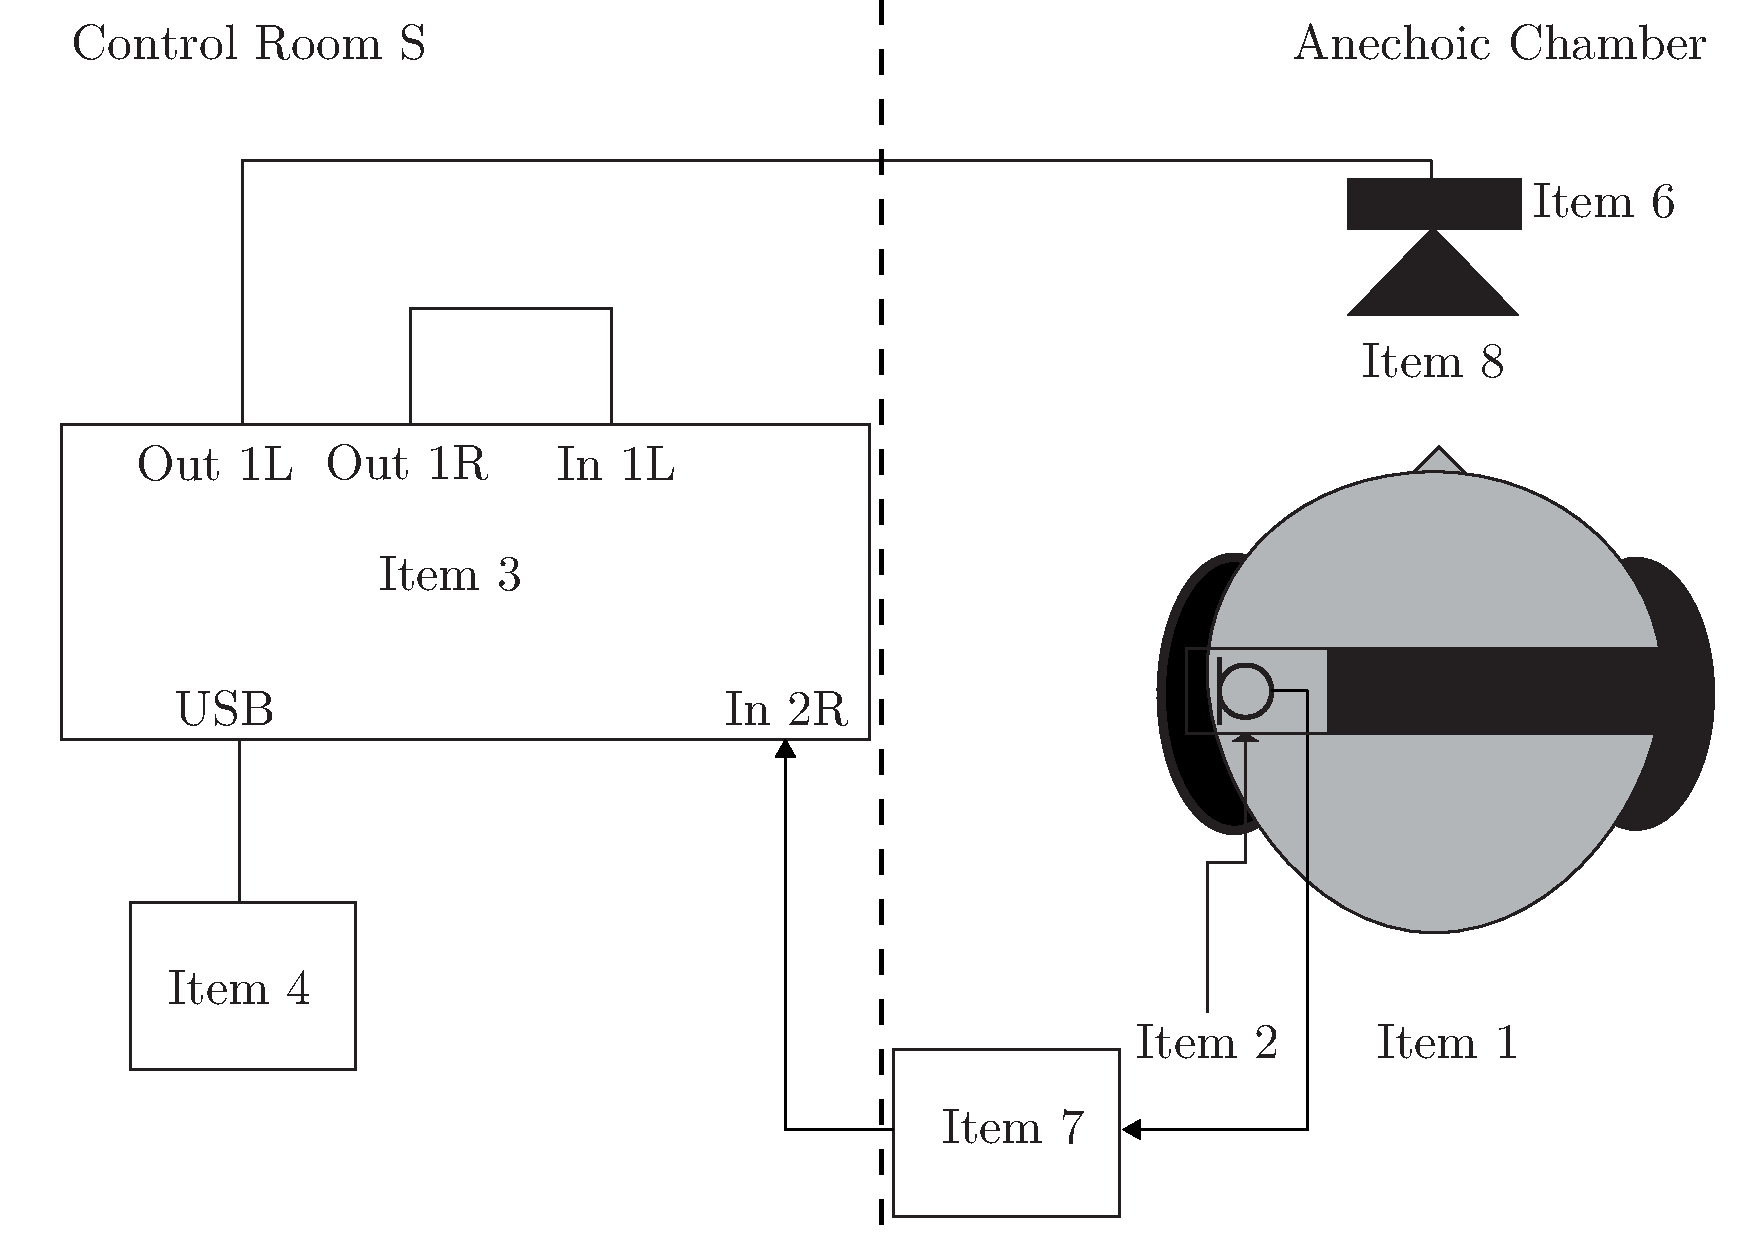
\includegraphics[width=0.8\textwidth]{../Journal/Experiments/TestofConsumerHeadphones/OtherBrandsDiagram.pdf}
	\caption{Diagram of the test set-up.}
	\label{OtherBrandsDiagram}
\end{figure}
\todoOliver{Change "ear" to "ear canal" It's kind of pointing at the microphone, avoidable? If the microphone symbol does not need explaining neither does the speaker symbol. The speaker symbol is not correct. The triangle should be on top of the bar. Directions on arrows! as for the microphone. It's RM[E] Fireface}

\subsection{Settings/Description}
\subsubsection{Control and calibration}
\begin{itemize}
	\item The speaker (6) is placed 1.6 meters from the HATS.
	\item The microphone in the Hats (2) is calibrated on the computer using Simulink\textsuperscript{\textregistered}.
	\begin{itemize} 
		\item Calibration is made @ 1 $k$Hz using the calibrator with adapter for the ear simulator. This should yield a signal of 95.6 dB. The measured intensity in MATLAB\textsuperscript{\textregistered} however was 78.12 so all measurements are multiplied by 7.48 to get a calibrated signal in Matlab\textsuperscript{\textregistered}.
	\end{itemize}
\end{itemize}

\subsubsection{Equipment settings}
\begin{itemize}
	\item This experiment is performed with a sampling rate of, $f_{s}$ = 48 $k$Hz. 
	\item In the mixing console on the computer 3 take care to turn on the "inst"-option. The following gain settings are present: 		
	\begin{itemize}
		\item Line level gain is 0 dB
		\item Ear Microphones has gain +30 dB set on the front of the RME
		%\item Ref Microphones has gain +48 dB
		%\item Speaker Microphones has gain +48 dB
	\end{itemize}
	\item All settings on the computer is set to 0 dBFS
\end{itemize}
	
	
\subsection{Pictures}
\begin{figure}[H]
	\centering
	\begin{subfigure}[b]{0.5\textwidth}
		\centering
		\includegraphics[width=\textwidth]{../Journal/Experiments/TestofConsumerHeadphones/Pictures/OtherBrandsSetupBack.jpg}
		\caption{Set-up from the back.}
	\end{subfigure}\qquad
	\begin{subfigure}[b]{0.4\textwidth}
		\includegraphics[width=\textwidth]{../Journal/Experiments/TestofConsumerHeadphones/Pictures/OtherBrandsSetupAngle.jpg}
		\caption{Set-up from an angle.}
		\vspace{2ex}
		\includegraphics[width=\textwidth]{../Journal/Experiments/TestofConsumerHeadphones/Pictures/OtherBrandsSetupSide.jpg}
		\caption{Set-up form the side.}
	\end{subfigure}
	\caption{The test set-up form different angles with the Bose QuietComfort 25 headphone.}
\label{fig:OtherBrandsPicture}
\end{figure}


\subsection{Procedure}
	\subsubsection{Set-up}
	\begin{enumerate}
		\item Connect cable from the RMEs "Out 1L" to the speakers "Line in"
		\item Connect cable from the RME's "Out 1R" to the RME's "In 1L"
		\item Connect cable from the microphone in the ear simulator (2) to the microphone power supply's (7) "Input"
		\item Connect cable from the microphone power supply's "Output" to the RME's "IN 2R"
		\item Connect USB-cable from the computer to the RME
	\end{enumerate}

	\subsubsection{Performing Experiment}
	\begin{enumerate}
		\item Open Simulink\textsuperscript{\textregistered} and open and run file \path{OtherBrands.xls}
		\begin{itemize} 
			\item The simulations outputs a speech signal at 0 dBFS over the span of 12 seconds
			\begin{itemize}
				\item [] The signal constructed using speech-files from "The Archimedes Project" by Bang \& Olufsen. \\
				The signal is composed of three seconds of the UK male anechoic sample followed by three seconds of silence, followed by the UK female anechoic sample, and ends with another three seconds of silence.
			\end{itemize}
			\item The simulation runs for 14 seconds
		\end{itemize}
		\item Rename generated file \path{GeneratedANC} according to headphone tested, and whether or not ANC was enabled. E.g. \path{Denonon[1].wav} for the first test of the Denon AH GC20 headhpone with ANC enabled. Names in \path{evaluatePerformance.m}-script is named accordingly.

	\end{enumerate}
	Perform this experiment five times for each headphone where the headphone is removed and remounted on the HATS between measurements. 
		
\subsection{Data Extraction}
\begin{enumerate}
	\item Open MATLAB\textsuperscript{\textregistered} and run script \path{evaluatePerformance.m}
\end{enumerate}

From performing the experiment, a list of files were generated, ten for each device tested; five with ANC enabled and five with ANC disabled. The list can be seen below, where [i] indicates the iteration of the experiment.

\begin{itemize}
	\item \path{Denonon[i].wav}			(Denon AH GC20 w/ ANC)
	\item \path{Denonoff[i].wav}		(Denon AH GC20 w/o ANC)
	\item \path{BoseQC15on[i].wav}		(Bose QuietComfort 15 w/ ANC)
	\item \path{BoseQC15off[i].wav}		(Bose QuietComfort 15 w/o ANC)
	\item \path{BoseQC25on[i].wav}		(Bose QuietComfort 25 w/ ANC)
	\item \path{BoseQC25off[i].wav}		(Bose QuietComfort 25 w/o ANC)
	\item \path{BOH8on[i].wav}			(B\&O BEOPLAY H8 w/ ANC)
	\item \path{BOH8off[i].wav}			(B\&O BEOPLAY H8 w/o ANC)
\end{itemize}


\subsection{Analysis}
The difference between the enabled and the disabled ANC is plotted on figures \ref{fig:BOH8Comp}, \ref{fig:QC15Comp}, \ref{fig:QC25Comp} and \ref{fig:DenonComp} for each headphone tested.
 The frequency responses are made using the method described in \autoref{sec:OctaveBank}. Only the part containing male voice is analysed. The averaging is made by putting all five recordings through the filter bank after one another. 

\begin{figure}[H]
	\centering
	\tikzsetnextfilename{BOH8Compare}
	% This file was created by matlab2tikz.
%
%The latest updates can be retrieved from
%  http://www.mathworks.com/matlabcentral/fileexchange/22022-matlab2tikz-matlab2tikz
%where you can also make suggestions and rate matlab2tikz.
%
\definecolor{mycolor1}{rgb}{0.00000,0.44700,0.74100}%
\definecolor{mycolor2}{rgb}{0.85000,0.32500,0.09800}%
%
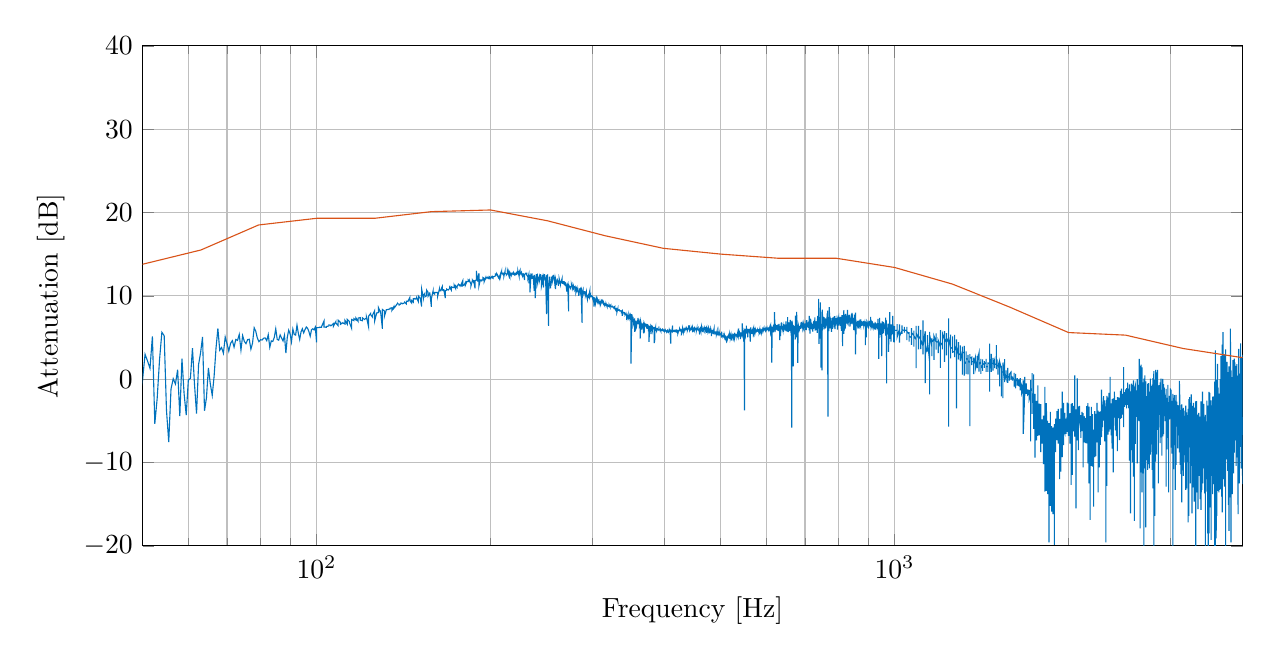
\begin{tikzpicture}

\begin{axis}[%
width=5.5in,
height=2.5in,
at={(1.011in,0.642in)},
scale only axis,
unbounded coords=jump,
xmode=log,
xmin=50,
xmax=4e+03,
xminorticks=true,
xlabel={Frequency [Hz]},
xmajorgrids,
xminorgrids,
ymin=-20,
ymax=40,
ylabel={Attenuation [dB]},
ymajorgrids,
axis background/.style={fill=white},
title style={font=\bfseries},
legend style={at={(0.03,0.03)},anchor=south west,legend cell align=left,align=left,draw=white!15!black}
]
\addplot [color=mycolor1,solid,forget plot]
  table[row sep=crcr]{%
0	-2.66\\
0.5	-2.54\\
1	-4.17\\
1.5	-6.63\\
2	-1.77\\
2.5	0.402\\
3	-1.51\\
3.5	6.5\\
4	3.26\\
4.5	3.21\\
5	-3.05\\
5.5	-0.676\\
6	-5.42\\
6.5	-2.1\\
7	-4.21\\
7.5	-5.78\\
8	-4.15\\
8.5	-7.68\\
9	-10.6\\
9.5	-8.08\\
10	-11.1\\
10.5	-17.2\\
11	-9.43\\
11.5	-11.6\\
12	-11.8\\
12.5	-9.78\\
13	-6.98\\
13.5	-6.74\\
14	-3.55\\
14.5	-6.07\\
15	-8.23\\
15.5	-7.26\\
16	-6.33\\
16.5	-4.21\\
17	-2.23\\
17.5	-0.158\\
18	-17.1\\
18.5	2.25\\
19	-4.18\\
19.5	-4.35\\
20	-2.24\\
20.5	-2.6\\
21	-0.613\\
21.5	-6.41\\
22	-1.93\\
22.5	-6.54\\
23	-9.3\\
23.5	-11.8\\
24	2.6\\
24.5	-0.344\\
25	3.3\\
25.5	-8.06\\
26	-3.7\\
26.5	2.75\\
27	-2.24\\
27.5	-3.79\\
28	-2.68\\
28.5	-0.965\\
29	-5.6\\
29.5	4.78\\
30	0.865\\
30.5	0.763\\
31	-0.0819\\
31.5	-0.0827\\
32	-1.85\\
32.5	-2.07\\
33	-4.81\\
33.5	2.07\\
34	-9.18\\
34.5	2.36\\
35	-4.61\\
35.5	0.939\\
36	-3.01\\
36.5	-11.1\\
37	-9.39\\
37.5	4.42\\
38	-2.06\\
38.5	-1.78\\
39	-8.43\\
39.5	-10.9\\
40	-15.2\\
40.5	-5.08\\
41	-3.7\\
41.5	-10.5\\
42	-3.1\\
42.5	-11.2\\
43	-3.07\\
43.5	6.29\\
44	2.43\\
44.5	-11.1\\
45	-1.29\\
45.5	-9.69\\
46	-0.631\\
46.5	-0.67\\
47	-4.06\\
47.5	-11.7\\
48	-0.404\\
48.5	4.21\\
49	4.72\\
49.5	-2.87\\
50	-0.1\\
50.5	2.98\\
51	2.18\\
51.5	1.29\\
52	5.14\\
52.5	-5.36\\
53	-2.29\\
53.5	2.34\\
54	5.62\\
54.5	5.21\\
55	-3.74\\
55.5	-7.56\\
56	-1.19\\
56.5	0.0528\\
57	-0.584\\
57.5	1.14\\
58	-4.45\\
58.5	2.45\\
59	-1.74\\
59.5	-4.31\\
60	-0.117\\
60.5	0.0906\\
61	3.71\\
61.5	-0.637\\
62	-4.14\\
62.5	1.74\\
63	3.14\\
63.5	5.07\\
64	-3.79\\
64.5	-2.24\\
65	1.34\\
65.5	-0.593\\
66	-1.95\\
66.5	0.372\\
67	3.72\\
67.5	6.09\\
68	3.47\\
68.5	3.79\\
69	3.11\\
69.5	5.05\\
70	4.28\\
70.5	3.36\\
71	4.29\\
71.5	4.62\\
72	3.84\\
72.5	4.76\\
73	4.65\\
73.5	5.36\\
74	3.48\\
74.5	5.23\\
75	4.54\\
75.5	4.26\\
76	4.75\\
76.5	4.78\\
77	3.6\\
77.5	4.31\\
78	6.16\\
78.5	5.75\\
79	4.93\\
79.5	4.5\\
80	4.73\\
80.5	4.69\\
81	4.92\\
81.5	4.94\\
82	4.62\\
82.5	5.34\\
83	3.81\\
83.5	4.59\\
84	4.52\\
84.5	5\\
85	6.04\\
85.5	4.77\\
86	4.68\\
86.5	5.3\\
87	4.94\\
87.5	4.58\\
88	5.27\\
88.5	3.12\\
89	5.03\\
89.5	5.88\\
90	5.44\\
90.5	4.48\\
91	6.01\\
91.5	5.35\\
92	5.29\\
92.5	6.48\\
93	5.49\\
93.5	4.76\\
94	5.67\\
94.5	6.04\\
95	5.55\\
95.5	5.95\\
96	6.26\\
96.5	6.09\\
97	5.71\\
97.5	5.15\\
98	5.92\\
98.5	6.04\\
99	5.91\\
99.5	6.25\\
100	4.41\\
100	6.17\\
101	6.19\\
101	6.22\\
102	6.23\\
102	6.29\\
103	6.97\\
103	6.24\\
104	6.23\\
104	6.32\\
105	6.38\\
105	6.51\\
106	6.45\\
106	6.43\\
107	6.68\\
107	6.37\\
108	6.9\\
108	6.74\\
109	6.41\\
109	7.07\\
110	6.8\\
110	6.58\\
111	6.76\\
111	6.74\\
112	6.61\\
112	7.04\\
113	6.6\\
113	7.17\\
114	6.92\\
114	6.8\\
115	6.09\\
115	7.15\\
116	7.02\\
116	7.27\\
117	7.09\\
117	7.33\\
118	6.93\\
118	7.33\\
119	7.38\\
119	7.08\\
120	7.01\\
120	7.36\\
121	7.18\\
121	7.17\\
122	7.33\\
122	7.42\\
123	6.32\\
123	7.54\\
124	7.87\\
124	7.76\\
125	7.43\\
125	7.68\\
126	8.19\\
126	6.95\\
127	7.87\\
127	7.94\\
128	7.99\\
128	8.56\\
129	8.03\\
129	8.24\\
130	6.03\\
130	8.36\\
131	8.19\\
131	7.5\\
132	8.29\\
132	8.32\\
133	8.37\\
133	8.36\\
134	8.42\\
134	8.5\\
135	8.57\\
135	8.24\\
136	8.67\\
136	8.49\\
137	8.77\\
137	8.76\\
138	9.07\\
138	9.05\\
139	9\\
139	8.9\\
140	9.05\\
140	9.13\\
141	9.08\\
141	9.06\\
142	9.17\\
142	9.23\\
143	9.03\\
143	9.36\\
144	9.32\\
144	9.38\\
145	9.8\\
145	9.42\\
146	9.15\\
146	9.43\\
147	9.23\\
147	9.64\\
148	9.68\\
148	9.61\\
149	9.63\\
149	9.75\\
150	9.31\\
150	9.98\\
151	9.72\\
151	9.86\\
152	8.72\\
152	10.8\\
153	9.84\\
153	10\\
154	10.3\\
154	9.88\\
155	10\\
155	10.7\\
156	10.4\\
156	9.96\\
157	10.3\\
157	10.4\\
158	8.67\\
158	9.66\\
159	10.5\\
159	10.3\\
160	10.2\\
160	10.4\\
161	10.4\\
161	10.4\\
162	10.4\\
162	9.95\\
163	10.7\\
163	10.6\\
164	10.6\\
164	10.7\\
165	11.1\\
165	10.7\\
166	10.6\\
166	10.8\\
167	9.73\\
167	10.6\\
168	10.7\\
168	10.8\\
169	10.7\\
169	10.7\\
170	10.9\\
170	11\\
171	10.7\\
171	11.1\\
172	11\\
172	11\\
173	11\\
173	11.3\\
174	10.9\\
174	11.2\\
175	11\\
175	11.1\\
176	11.4\\
176	11.4\\
177	11.2\\
177	11.3\\
178	11.2\\
178	11.4\\
179	11.8\\
179	11.2\\
180	11.3\\
180	11.3\\
181	11.6\\
181	11.3\\
182	11.7\\
182	11.7\\
183	11.7\\
183	11.9\\
184	11.7\\
184	11.8\\
185	11.4\\
185	11.2\\
186	11.8\\
186	11.9\\
187	11.6\\
187	11.9\\
188	10.9\\
188	11.8\\
189	11.9\\
189	13\\
190	11.7\\
190	11.9\\
191	12.7\\
191	11.2\\
192	11.9\\
192	11.9\\
193	11.8\\
193	11.9\\
194	11.9\\
194	12.2\\
195	12.1\\
195	11.7\\
196	12.1\\
196	12\\
197	12.2\\
197	12.2\\
198	12.1\\
198	12.2\\
199	12.1\\
199	12.3\\
200	12.2\\
200	12.1\\
201	12.3\\
201	12.2\\
202	12.1\\
202	12.3\\
203	12.3\\
203	12.3\\
204	12.4\\
204	12.6\\
205	12.5\\
205	12.6\\
206	12.3\\
206	12.4\\
207	12.1\\
207	12.2\\
208	12.6\\
208	12.3\\
209	12.9\\
209	12.8\\
210	12.6\\
210	12.7\\
211	12.7\\
211	12.4\\
212	13\\
212	12.7\\
213	12.6\\
213	12.5\\
214	12.7\\
214	13\\
215	12.5\\
215	12.8\\
216	12.3\\
216	12.8\\
217	12.5\\
217	12.7\\
218	12.7\\
218	12.6\\
219	12.8\\
219	12.6\\
220	12.5\\
220	12.7\\
221	12.7\\
221	12.6\\
222	12.8\\
222	12.6\\
223	12.7\\
223	13\\
224	12.4\\
224	12.8\\
225	13.1\\
225	12.6\\
226	12.8\\
226	12.7\\
227	12.4\\
227	12.6\\
228	12.4\\
228	12.7\\
229	11.9\\
229	12.5\\
230	12.7\\
230	12.7\\
231	12.7\\
231	12.5\\
232	12.3\\
232	12.1\\
233	12.6\\
233	11.5\\
234	12.5\\
234	10.4\\
235	12.7\\
235	12.3\\
236	12.5\\
236	12.1\\
237	12.1\\
237	12.4\\
238	10.6\\
238	12.5\\
239	11.8\\
239	9.73\\
240	12.6\\
240	12.3\\
241	12.5\\
241	11.5\\
242	12.1\\
242	12.1\\
243	12.4\\
243	11.8\\
244	12.3\\
244	12.6\\
245	11.8\\
245	11.2\\
246	11.8\\
246	12.5\\
247	11\\
247	12.4\\
248	12.1\\
248	12.6\\
249	11.8\\
249	12.2\\
250	7.81\\
250	12.4\\
251	12.5\\
251	12.3\\
252	6.38\\
252	10.6\\
253	12.3\\
253	11.9\\
254	10.9\\
254	11\\
255	12.3\\
255	12.1\\
256	12.3\\
256	11.8\\
257	12.3\\
257	12.5\\
258	11.9\\
258	11.8\\
259	10.8\\
259	12.1\\
260	11.6\\
260	11.3\\
261	11.9\\
261	11.9\\
262	11.6\\
262	11.2\\
263	11.8\\
263	12\\
264	11.5\\
264	11.6\\
265	11.6\\
265	11.7\\
266	12.1\\
266	11.5\\
267	11.5\\
267	11.7\\
268	11.7\\
268	11.4\\
269	11.3\\
269	11.6\\
270	11.5\\
270	11.5\\
271	10.5\\
271	11.1\\
272	11.4\\
272	11.2\\
273	8.13\\
273	11.3\\
274	11.1\\
274	11.1\\
275	10.9\\
275	11.1\\
276	11.1\\
276	11.4\\
277	11\\
277	11.1\\
278	10.9\\
278	11.3\\
279	11\\
279	11\\
280	11.1\\
280	10.7\\
281	10.9\\
281	10.4\\
282	10.8\\
282	10.6\\
283	10.8\\
283	10.6\\
284	10.3\\
284	10\\
285	10.9\\
285	10.6\\
286	10.8\\
286	10.4\\
287	10.7\\
287	10.3\\
288	6.75\\
288	10.4\\
289	10.7\\
289	10.1\\
290	10.5\\
290	10.5\\
291	10.5\\
291	10.3\\
292	10.4\\
292	10.1\\
293	10.5\\
293	10.1\\
294	9.68\\
294	9.97\\
295	10.1\\
295	9.83\\
296	9.76\\
296	10.1\\
297	10.6\\
297	9.82\\
298	10.1\\
298	9.92\\
299	9.9\\
299	10\\
300	9.96\\
300	9.79\\
301	9.47\\
301	9.82\\
302	9.71\\
302	8.71\\
303	9.49\\
303	9.65\\
304	9.5\\
304	9.13\\
305	9.54\\
305	9.59\\
306	9.32\\
306	9.63\\
307	9.33\\
307	9.46\\
308	9.52\\
308	9.33\\
309	9.05\\
309	9.28\\
310	9.34\\
310	8.93\\
311	9.17\\
311	9.42\\
312	9.26\\
312	9.3\\
313	9.12\\
313	9.29\\
314	9.06\\
314	9.16\\
315	8.91\\
315	9.08\\
316	9.07\\
316	8.9\\
317	8.84\\
317	9.03\\
318	8.76\\
318	8.85\\
319	8.86\\
319	8.89\\
320	8.81\\
320	8.74\\
321	8.7\\
321	8.87\\
322	8.64\\
322	8.8\\
323	8.91\\
323	8.76\\
324	8.68\\
324	8.72\\
325	8.75\\
325	8.68\\
326	8.63\\
326	8.63\\
327	8.67\\
327	8.57\\
328	8.69\\
328	8.47\\
329	8.32\\
329	8.45\\
330	8.48\\
330	8.4\\
331	8.41\\
331	8.07\\
332	8.41\\
332	8.33\\
333	8.32\\
333	8.27\\
334	8.3\\
334	8.24\\
335	8.23\\
335	8.17\\
336	8.19\\
336	8.17\\
337	8.15\\
337	8.07\\
338	8.2\\
338	7.59\\
339	8.1\\
339	7.98\\
340	7.96\\
340	8.01\\
341	7.98\\
341	7.81\\
342	7.81\\
342	7.71\\
343	7.86\\
343	7.81\\
344	7.8\\
344	7.11\\
345	7.68\\
345	7.41\\
346	7.75\\
346	7.37\\
347	7.2\\
347	7.45\\
348	7.68\\
348	7.53\\
349	7.67\\
349	7.26\\
350	7.07\\
350	1.86\\
351	7.35\\
351	7.79\\
352	7.36\\
352	7.04\\
353	7.23\\
353	6.49\\
354	6.77\\
354	7.13\\
355	7.2\\
355	5.67\\
356	6.5\\
356	6.43\\
357	7.01\\
357	6.07\\
358	6.29\\
358	6.49\\
359	6.93\\
359	6.76\\
360	7.35\\
360	6.85\\
361	7\\
361	6.74\\
362	6.83\\
362	6.56\\
363	6.91\\
363	4.86\\
364	6.6\\
364	6.85\\
365	6.49\\
365	5.94\\
366	6.69\\
366	6.22\\
367	6.39\\
367	6.56\\
368	5.5\\
368	6.33\\
369	6.02\\
369	6.69\\
370	6.44\\
370	6.32\\
371	6.49\\
371	6.6\\
372	6.57\\
372	6.47\\
373	6.04\\
373	6.5\\
374	6.54\\
374	6.54\\
375	6.35\\
375	5.74\\
376	6.43\\
376	4.48\\
377	6.25\\
377	6.29\\
378	6.32\\
378	6.32\\
379	5.4\\
379	6.42\\
380	6.29\\
380	6.27\\
381	5.92\\
381	6.32\\
382	6.22\\
382	6.09\\
383	6.03\\
383	6.15\\
384	6.18\\
384	4.33\\
385	4.88\\
385	5.78\\
386	6.16\\
386	6.11\\
387	5.89\\
387	6.06\\
388	6.02\\
388	6.06\\
389	6.03\\
389	5.96\\
390	6.12\\
390	5.97\\
391	5.88\\
391	5.93\\
392	5.97\\
392	5.97\\
393	5.9\\
393	5.99\\
394	5.79\\
394	5.96\\
395	5.85\\
395	5.84\\
396	5.93\\
396	5.86\\
397	5.83\\
397	5.85\\
398	5.82\\
398	5.92\\
399	5.82\\
399	5.8\\
400	5.88\\
400	5.74\\
401	5.87\\
401	5.76\\
402	5.77\\
402	5.79\\
403	5.67\\
403	5.73\\
404	5.82\\
404	5.74\\
405	5.82\\
405	5.66\\
406	5.61\\
406	5.75\\
407	5.79\\
407	5.72\\
408	5.7\\
408	5.9\\
409	5.73\\
409	5.72\\
410	4.26\\
410	5.84\\
411	5.78\\
411	5.79\\
412	5.7\\
412	5.81\\
413	6.43\\
413	5.71\\
414	5.77\\
414	5.75\\
415	5.72\\
415	5.84\\
416	5.86\\
416	5.75\\
417	5.73\\
417	5.75\\
418	5.7\\
418	5.85\\
419	5.8\\
419	5.8\\
420	5.68\\
420	5.79\\
421	5.7\\
421	5.84\\
422	5.77\\
422	5.53\\
423	5.78\\
423	5.84\\
424	5.81\\
424	5.8\\
425	5.86\\
425	6.02\\
426	5.86\\
426	5.86\\
427	5.75\\
427	5.9\\
428	5.83\\
428	5.68\\
429	5.93\\
429	5.63\\
430	5.85\\
430	6.03\\
431	5.74\\
431	5.92\\
432	6.01\\
432	5.84\\
433	5.85\\
433	6.02\\
434	5.92\\
434	5.88\\
435	6.05\\
435	5.94\\
436	6\\
436	5.95\\
437	5.94\\
437	6.03\\
438	5.86\\
438	5.83\\
439	6.04\\
439	5.98\\
440	6.12\\
440	6.04\\
441	6.02\\
441	6.48\\
442	6.1\\
442	5.89\\
443	6.07\\
443	6.1\\
444	6.08\\
444	5.99\\
445	6.1\\
445	6.17\\
446	5.97\\
446	6.03\\
447	6.24\\
447	6.02\\
448	6.07\\
448	5.84\\
449	5.96\\
449	6.16\\
450	5.65\\
450	5.93\\
451	6.28\\
451	5.9\\
452	6.08\\
452	6.09\\
453	5.98\\
453	5.98\\
454	6.06\\
454	5.79\\
455	6.08\\
455	5.94\\
456	5.92\\
456	5.99\\
457	6.11\\
457	6.01\\
458	5.89\\
458	5.93\\
459	6.01\\
459	6.02\\
460	5.36\\
460	6.05\\
461	6.13\\
461	6.12\\
462	5.83\\
462	6\\
463	6.26\\
463	5.9\\
464	6.04\\
464	6.39\\
465	5.94\\
465	5.66\\
466	6.12\\
466	5.97\\
467	5.84\\
467	6.05\\
468	6.18\\
468	6.1\\
469	6.05\\
469	5.91\\
470	6.24\\
470	5.83\\
471	6\\
471	5.98\\
472	5.92\\
472	5.88\\
473	6.11\\
473	5.56\\
474	5.97\\
474	5.87\\
475	6.19\\
475	5.89\\
476	6.01\\
476	5.62\\
477	5.76\\
477	6.11\\
478	5.93\\
478	5.89\\
479	5.51\\
479	5.84\\
480	6\\
480	5.65\\
481	5.72\\
481	6.01\\
482	5.79\\
482	5.17\\
483	5.71\\
483	5.71\\
484	5.71\\
484	5.84\\
485	5.86\\
485	5.51\\
486	5.49\\
486	5.71\\
487	5.99\\
487	5.59\\
488	5.7\\
488	5.71\\
489	5.36\\
489	5.66\\
490	5.68\\
490	5.71\\
491	5.4\\
491	5.62\\
492	5.66\\
492	5.45\\
493	5.72\\
493	5.46\\
494	5.48\\
494	5.25\\
495	5.57\\
495	5.56\\
496	5.42\\
496	5.54\\
497	5.46\\
497	5.75\\
498	5.48\\
498	5.38\\
499	5.37\\
499	5.36\\
500	5.42\\
500	5.35\\
501	5.33\\
501	5.31\\
502	4.98\\
502	5.7\\
503	5.18\\
503	5.26\\
504	5.19\\
504	5.18\\
505	5.22\\
505	5.06\\
506	5.16\\
506	5.1\\
507	5.14\\
507	5.15\\
508	4.99\\
508	5.27\\
509	5.07\\
509	4.94\\
510	5.02\\
510	4.94\\
511	4.74\\
511	5.08\\
512	5.01\\
512	4.88\\
513	4.96\\
513	5.02\\
514	5.1\\
514	4.83\\
515	5.04\\
515	5.08\\
516	5.23\\
516	5.07\\
517	5\\
517	5.14\\
518	5.08\\
518	5.1\\
519	5.14\\
519	5.44\\
520	5.21\\
520	4.95\\
521	5.21\\
521	5.1\\
522	5.05\\
522	5.33\\
523	4.62\\
523	4.98\\
524	5.09\\
524	5.25\\
525	5.17\\
525	5.14\\
526	4.95\\
526	5.31\\
527	5.22\\
527	5.1\\
528	5.25\\
528	5.27\\
529	5.56\\
529	4.98\\
530	5.23\\
530	5.27\\
531	5.24\\
531	5.31\\
532	5.24\\
532	5.21\\
533	5.14\\
533	5.36\\
534	5.41\\
534	5.21\\
535	5.49\\
535	5.36\\
536	5.15\\
536	5.25\\
537	5.5\\
537	5.1\\
538	5.15\\
538	5.66\\
539	5.5\\
539	5.35\\
540	5.35\\
540	5.52\\
541	5.37\\
541	4.8\\
542	5.28\\
542	5.61\\
543	5.27\\
543	5.47\\
544	5.43\\
544	5.47\\
545	5.06\\
545	6.69\\
546	5.72\\
546	5.34\\
547	5.54\\
547	5.65\\
548	5.44\\
548	4.49\\
549	5.85\\
549	5.67\\
550	-3.76\\
550	5.78\\
551	5.62\\
551	5.6\\
552	5.35\\
552	6.04\\
553	5.59\\
553	5.61\\
554	5.8\\
554	6.43\\
555	5.52\\
555	5.49\\
556	6.04\\
556	5.42\\
557	5.7\\
557	5.02\\
558	5.97\\
558	5.76\\
559	6.03\\
559	5.69\\
560	5.69\\
560	5.9\\
561	5.5\\
561	5.7\\
562	6.03\\
562	5.21\\
563	4.49\\
563	5.81\\
564	5.71\\
564	6.21\\
565	5.49\\
565	5.94\\
566	5.56\\
566	5.42\\
567	5.75\\
567	5.76\\
568	5.91\\
568	5.7\\
569	5.5\\
569	5.72\\
570	5.96\\
570	5.49\\
571	5.67\\
571	5.89\\
572	5.76\\
572	5.64\\
573	5.81\\
573	5.96\\
574	5.86\\
574	5.61\\
575	5.85\\
575	5.89\\
576	5.72\\
576	5.58\\
577	5.96\\
577	5.82\\
578	5.79\\
578	5.8\\
579	5.79\\
579	6.04\\
580	5.68\\
580	5.96\\
581	5.86\\
581	5.88\\
582	5.6\\
582	5.65\\
583	5.99\\
583	5.67\\
584	5.89\\
584	5.82\\
585	5.89\\
585	5.37\\
586	5.78\\
586	5.88\\
587	5.9\\
587	5.9\\
588	5.69\\
588	5.73\\
589	5.82\\
589	5.84\\
590	5.96\\
590	5.9\\
591	5.78\\
591	5.87\\
592	5.88\\
592	5.85\\
593	5.99\\
593	5.85\\
594	6.02\\
594	5.92\\
595	5.93\\
595	5.98\\
596	5.91\\
596	5.92\\
597	6.03\\
597	6\\
598	5.97\\
598	5.97\\
599	5.95\\
599	5.92\\
600	6.04\\
600	5.93\\
601	6.07\\
601	5.91\\
602	5.96\\
602	5.98\\
603	6.01\\
603	6.04\\
604	5.96\\
604	6.02\\
605	6.02\\
605	6.15\\
606	6.16\\
606	6.11\\
607	6.1\\
607	6.05\\
608	6.21\\
608	6.11\\
609	5.9\\
609	6\\
610	6.23\\
610	6.13\\
611	5.14\\
611	6.45\\
612	6.06\\
612	6.23\\
613	6.2\\
613	1.98\\
614	4.96\\
614	6.1\\
615	6.16\\
615	6.07\\
616	6.22\\
616	5.96\\
617	6.07\\
617	5.62\\
618	6.52\\
618	5.84\\
619	6.27\\
619	6.45\\
620	5.98\\
620	8.03\\
621	5.64\\
621	6.42\\
622	5.86\\
622	6.62\\
623	5.92\\
623	6.44\\
624	6.36\\
624	6.23\\
625	6.13\\
625	6.17\\
626	6.47\\
626	6.36\\
627	6.35\\
627	5.82\\
628	6.55\\
628	6.42\\
629	6.08\\
629	5.96\\
630	5.82\\
630	5.75\\
631	6.63\\
631	6.29\\
632	6.06\\
632	6.12\\
633	5.96\\
633	4.69\\
634	6.39\\
634	5.8\\
635	6.25\\
635	5.17\\
636	6.36\\
636	5.98\\
637	6.82\\
637	6.12\\
638	6.28\\
638	6.19\\
639	6.09\\
639	6.04\\
640	6.39\\
640	6\\
641	5.81\\
641	6.27\\
642	5.68\\
642	5.74\\
643	6.08\\
643	6.6\\
644	6.11\\
644	6.4\\
645	6.22\\
645	6.39\\
646	6.34\\
646	6.03\\
647	6.53\\
647	6.32\\
648	6.36\\
648	5.82\\
649	6.08\\
649	6.94\\
650	6.03\\
650	6.42\\
651	5.73\\
651	6.27\\
652	6.02\\
652	5.9\\
653	6.33\\
653	7.45\\
654	5.67\\
654	5.84\\
655	5.87\\
655	5.65\\
656	6.66\\
656	6.8\\
657	5.8\\
657	6.16\\
658	5.76\\
658	5.82\\
659	6.59\\
659	6.04\\
660	7.11\\
660	5.86\\
661	6.45\\
661	6.46\\
662	6.4\\
662	5.61\\
663	5.11\\
663	6.92\\
664	-5.81\\
664	5.57\\
665	5.6\\
665	7.02\\
666	5.76\\
666	4.88\\
667	5.14\\
667	6.54\\
668	1.53\\
668	6.41\\
669	6.39\\
669	5.77\\
670	6.12\\
670	5.39\\
671	6.36\\
671	5.64\\
672	5.48\\
672	6.07\\
673	5.71\\
673	4.75\\
674	5.41\\
674	7.62\\
675	5.08\\
675	5.7\\
676	6.16\\
676	5\\
677	5.9\\
677	8.06\\
678	5.95\\
678	6.12\\
679	6.23\\
679	5.94\\
680	5.63\\
680	1.95\\
681	6.08\\
681	6.46\\
682	5.73\\
682	6.39\\
683	6.18\\
683	5.62\\
684	6.06\\
684	5.82\\
685	6.38\\
685	6.24\\
686	6.01\\
686	6.05\\
687	6.25\\
687	6.09\\
688	6.12\\
688	6.35\\
689	6.37\\
689	6.49\\
690	6.39\\
690	6.86\\
691	6.22\\
691	6.26\\
692	6.16\\
692	6.07\\
693	6.38\\
693	6.29\\
694	6.75\\
694	6.04\\
695	6.2\\
695	6.41\\
696	6.21\\
696	6.57\\
697	6.36\\
697	6.37\\
698	6.47\\
698	6.56\\
699	6.32\\
699	6.36\\
700	6.68\\
700	6.3\\
701	6.35\\
701	6.36\\
702	6.25\\
702	5.91\\
703	6.38\\
703	6.52\\
704	6.34\\
704	6.74\\
705	6.18\\
705	7.09\\
706	6.37\\
706	6.38\\
707	6.49\\
707	6.74\\
708	6.5\\
708	6.58\\
709	6.6\\
709	6.21\\
710	6.91\\
710	6.15\\
711	6.4\\
711	6.84\\
712	5.86\\
712	7.59\\
713	6.52\\
713	6.29\\
714	5.47\\
714	7.18\\
715	6.42\\
715	7.26\\
716	6.09\\
716	7.16\\
717	6.47\\
717	6.02\\
718	6.4\\
718	6.31\\
719	6.54\\
719	6.77\\
720	6.3\\
720	6.18\\
721	5.88\\
721	6.49\\
722	5.71\\
722	6.37\\
723	6.5\\
723	6.59\\
724	6.3\\
724	6.04\\
725	6.97\\
725	6.8\\
726	6.51\\
726	6.7\\
727	7.1\\
727	6.12\\
728	6.98\\
728	7.41\\
729	5.81\\
729	6.36\\
730	6.46\\
730	6.67\\
731	6.7\\
731	6.51\\
732	5.89\\
732	6.46\\
733	6.93\\
733	6.38\\
734	6.75\\
734	6.96\\
735	6.67\\
735	5.56\\
736	7.59\\
736	6.7\\
737	6.92\\
737	6.24\\
738	7.04\\
738	6.06\\
739	7.47\\
739	9.64\\
740	4.22\\
740	6.43\\
741	7.12\\
741	5.87\\
742	5.18\\
742	7.43\\
743	6.91\\
743	5.36\\
744	4.88\\
744	9.22\\
745	6.35\\
745	6.16\\
746	5.88\\
746	1.39\\
747	6.63\\
747	2.26\\
748	6.64\\
748	4.35\\
749	4.2\\
749	1.04\\
750	8.35\\
750	6.33\\
751	6.64\\
751	7.78\\
752	6.27\\
752	6.34\\
753	7.36\\
753	6.73\\
754	6.43\\
754	6.58\\
755	7.43\\
755	5.98\\
756	7.27\\
756	7.06\\
757	6.99\\
757	7.18\\
758	6.78\\
758	6.19\\
759	6.17\\
759	7.29\\
760	6.81\\
760	6.43\\
761	6.64\\
761	7.26\\
762	6.67\\
762	6.62\\
763	6.9\\
763	6.84\\
764	6.3\\
764	7.28\\
765	7.9\\
765	6.13\\
766	8.22\\
766	7.19\\
767	-4.51\\
767	6.66\\
768	7.01\\
768	6.02\\
769	6.29\\
769	7.45\\
770	5.77\\
770	6.26\\
771	8.63\\
771	6.32\\
772	6.1\\
772	7.99\\
773	6.92\\
773	6.24\\
774	6.22\\
774	7.35\\
775	6.7\\
775	7.08\\
776	6.9\\
776	6.4\\
777	7.31\\
777	6.19\\
778	5.68\\
778	6.63\\
779	6.7\\
779	6.84\\
780	6.82\\
780	7.02\\
781	6.7\\
781	6.03\\
782	7.4\\
782	6.7\\
783	6.98\\
783	7\\
784	7.13\\
784	6.56\\
785	6.86\\
785	7.05\\
786	6.99\\
786	6.22\\
787	7.1\\
787	6.61\\
788	6.87\\
788	7.56\\
789	7.02\\
789	6.01\\
790	6.84\\
790	7.25\\
791	6.98\\
791	6.93\\
792	7.31\\
792	6.73\\
793	7.09\\
793	6.96\\
794	6.99\\
794	6.96\\
795	7.12\\
795	7.02\\
796	7.08\\
796	7.34\\
797	7.26\\
797	5.95\\
798	7.11\\
798	7.12\\
799	6.86\\
799	7.09\\
800	7.31\\
800	7.01\\
801	7.48\\
801	6.42\\
802	7.22\\
802	7.02\\
803	7.12\\
803	6.84\\
804	7.27\\
804	7.22\\
805	6.57\\
805	7.42\\
806	6.75\\
806	6.4\\
807	7.12\\
807	6.9\\
808	6.97\\
808	7.46\\
809	5.79\\
809	6.88\\
810	6.94\\
810	6.86\\
811	7.67\\
811	6.43\\
812	7.12\\
812	7.44\\
813	3.95\\
813	6.6\\
814	7.69\\
814	5.99\\
815	6.8\\
815	7.36\\
816	6.37\\
816	5.73\\
817	8.27\\
817	5.44\\
818	7.15\\
818	7.04\\
819	5.82\\
819	6.78\\
820	7.26\\
820	7.73\\
821	7.15\\
821	6.11\\
822	6.18\\
822	6.97\\
823	7.08\\
823	7.82\\
824	7.03\\
824	7.04\\
825	6.67\\
825	7.08\\
826	7.38\\
826	6.99\\
827	6.9\\
827	7.28\\
828	6.69\\
828	7.14\\
829	8.32\\
829	6.93\\
830	7.08\\
830	6.87\\
831	6.75\\
831	7.38\\
832	6.71\\
832	6.86\\
833	6.99\\
833	7.11\\
834	6.88\\
834	6.86\\
835	7.71\\
835	7.41\\
836	6.82\\
836	7.14\\
837	6.97\\
837	6.29\\
838	6.83\\
838	7\\
839	7.17\\
839	6.72\\
840	7.14\\
840	7.16\\
841	6.6\\
841	7.02\\
842	6.71\\
842	6.85\\
843	6.91\\
843	6.99\\
844	6.77\\
844	7.95\\
845	6.69\\
845	6.86\\
846	7.77\\
846	6.91\\
847	6.84\\
847	6.58\\
848	7.37\\
848	6.85\\
849	6.79\\
849	7\\
850	5.94\\
850	5.89\\
851	6.66\\
851	7.31\\
852	6.63\\
852	6.6\\
853	6.82\\
853	7.74\\
854	6.82\\
854	7.13\\
855	7.32\\
855	6.56\\
856	2.96\\
856	7.98\\
857	6.49\\
857	6.77\\
858	5.36\\
858	6.59\\
859	6.67\\
859	6.82\\
860	6.62\\
860	6.44\\
861	6.73\\
861	6.65\\
862	6.51\\
862	6.65\\
863	7\\
863	6.81\\
864	6.66\\
864	6.89\\
865	6.91\\
865	6.75\\
866	6.85\\
866	6.88\\
867	6.86\\
867	6.86\\
868	6.61\\
868	6.07\\
869	6.7\\
869	7.06\\
870	6.69\\
870	6.45\\
871	6.91\\
871	6.44\\
872	6.37\\
872	6.65\\
873	6.5\\
873	6.66\\
874	6.67\\
874	7.18\\
875	6.5\\
875	6.57\\
876	6.73\\
876	6.75\\
877	6.38\\
877	6.89\\
878	6.63\\
878	6.46\\
879	6.72\\
879	6.76\\
880	6.71\\
880	6.75\\
881	6.77\\
881	6.53\\
882	6.49\\
882	6.55\\
883	6.98\\
883	6.44\\
884	6.71\\
884	6.87\\
885	6.49\\
885	6.48\\
886	6.63\\
886	6.58\\
887	6.53\\
887	6.63\\
888	6.55\\
888	6.35\\
889	6.72\\
889	6.94\\
890	6.36\\
890	4.08\\
891	6.85\\
891	6.78\\
892	6.52\\
892	6.62\\
893	6.75\\
893	6.63\\
894	5\\
894	6.74\\
895	6.62\\
895	6.75\\
896	6.73\\
896	6.71\\
897	6.44\\
897	6.59\\
898	6.67\\
898	6.59\\
899	6.7\\
899	7.01\\
900	6.64\\
900	6.53\\
901	6.74\\
901	6.4\\
902	6.07\\
902	6.39\\
903	6.82\\
903	6.56\\
904	6.53\\
904	6.73\\
905	6.43\\
905	6.92\\
906	6.93\\
906	6.76\\
907	6.42\\
907	6.56\\
908	6.48\\
908	6.25\\
909	6.82\\
909	7.48\\
910	6.48\\
910	6.42\\
911	6.72\\
911	6.35\\
912	6.49\\
912	6.42\\
913	6.2\\
913	6.44\\
914	6.67\\
914	6.36\\
915	6.35\\
915	6.8\\
916	6.75\\
916	6.35\\
917	6.47\\
917	6.57\\
918	6.37\\
918	6.46\\
919	6.32\\
919	6.47\\
920	6.41\\
920	6.52\\
921	6.59\\
921	6.3\\
922	6.38\\
922	6.55\\
923	6.03\\
923	6.23\\
924	6.69\\
924	6.6\\
925	5.95\\
925	6.46\\
926	6.41\\
926	6.39\\
927	6.29\\
927	6.65\\
928	6.37\\
928	6.6\\
929	6.54\\
929	6.24\\
930	6.25\\
930	6.53\\
931	6.36\\
931	6.32\\
932	6.22\\
932	6.44\\
933	6.72\\
933	6.17\\
934	6.45\\
934	6.26\\
935	6.01\\
935	6.29\\
936	6.21\\
936	7.23\\
937	6.03\\
937	6.37\\
938	6.17\\
938	6.7\\
939	6.5\\
939	2.42\\
940	6.17\\
940	6.17\\
941	6.52\\
941	6.22\\
942	6.34\\
942	7.35\\
943	6.27\\
943	5.35\\
944	5.97\\
944	6.36\\
945	6.07\\
945	6.41\\
946	5.99\\
946	5.32\\
947	6.61\\
947	6.68\\
948	5.02\\
948	5.07\\
949	6.65\\
949	6.39\\
950	5.2\\
950	2.75\\
951	5.91\\
951	6.67\\
952	6\\
952	6.93\\
953	5.44\\
953	5.81\\
954	5.84\\
954	6.21\\
955	6.2\\
955	6.54\\
956	5.53\\
956	5.64\\
957	6.87\\
957	6.05\\
958	6.48\\
958	6\\
959	6.16\\
959	6.12\\
960	6.51\\
960	6.31\\
961	6.2\\
961	6.14\\
962	6.56\\
962	6.1\\
963	6.43\\
963	6.73\\
964	5.52\\
964	6.17\\
965	5.21\\
965	7.39\\
966	6.4\\
966	6.35\\
967	6.83\\
967	5.72\\
968	6.12\\
968	7.04\\
969	-0.515\\
969	6.01\\
970	5.31\\
970	5.97\\
971	5.9\\
971	6\\
972	6.16\\
972	6.17\\
973	5.73\\
973	5.78\\
974	6.62\\
974	6.17\\
975	6.25\\
975	6.67\\
976	3.27\\
976	6.6\\
977	4.18\\
977	6.09\\
978	5.4\\
978	5.83\\
979	5.87\\
979	5.92\\
980	4.82\\
980	5.43\\
981	8.03\\
981	5\\
982	6.05\\
982	4.92\\
983	5.73\\
983	6.48\\
984	5.93\\
984	5.73\\
985	5.76\\
985	5.69\\
986	4.51\\
986	5.68\\
987	5.66\\
987	6.56\\
988	5.79\\
988	5.67\\
989	5.28\\
989	5.75\\
990	5.79\\
990	5.64\\
991	5.74\\
991	5.65\\
992	5.86\\
992	5.96\\
993	5.98\\
993	7.59\\
994	5.77\\
994	5.7\\
995	5.44\\
995	6.1\\
996	5.77\\
996	4.45\\
997	5.95\\
997	5.67\\
998	5.73\\
998	6.35\\
999	4.41\\
999	6.08\\
1e+03	5.53\\
1e+03	5.9\\
1e+03	5.49\\
1e+03	5.74\\
1e+03	5.76\\
1e+03	5.31\\
1e+03	5.63\\
1e+03	6.35\\
1e+03	5.57\\
1e+03	5.35\\
1e+03	5.86\\
1.01e+03	5.84\\
1.01e+03	5.93\\
1.01e+03	5.82\\
1.01e+03	5.63\\
1.01e+03	5.67\\
1.01e+03	6.06\\
1.01e+03	5.77\\
1.01e+03	5.58\\
1.01e+03	5.49\\
1.01e+03	5.43\\
1.01e+03	5.49\\
1.01e+03	5.75\\
1.01e+03	5.89\\
1.01e+03	6.6\\
1.01e+03	5.75\\
1.01e+03	5.8\\
1.01e+03	5.55\\
1.01e+03	6.04\\
1.01e+03	5.37\\
1.01e+03	5.04\\
1.02e+03	6.04\\
1.02e+03	5.53\\
1.02e+03	5.22\\
1.02e+03	5.92\\
1.02e+03	5.87\\
1.02e+03	5.59\\
1.02e+03	5.41\\
1.02e+03	5.82\\
1.02e+03	6.38\\
1.02e+03	5.57\\
1.02e+03	5.98\\
1.02e+03	6.07\\
1.02e+03	6.26\\
1.02e+03	5.65\\
1.02e+03	5.95\\
1.02e+03	4.38\\
1.02e+03	5.86\\
1.02e+03	6.56\\
1.02e+03	6\\
1.02e+03	5.14\\
1.03e+03	5.8\\
1.03e+03	5.45\\
1.03e+03	5.43\\
1.03e+03	6.09\\
1.03e+03	6.45\\
1.03e+03	6.1\\
1.03e+03	5.65\\
1.03e+03	5.8\\
1.03e+03	5.5\\
1.03e+03	6.11\\
1.03e+03	6.29\\
1.03e+03	6.05\\
1.03e+03	5.88\\
1.03e+03	6.09\\
1.03e+03	5.57\\
1.03e+03	5.7\\
1.03e+03	5.76\\
1.03e+03	6.03\\
1.03e+03	6.05\\
1.03e+03	5.91\\
1.04e+03	5.85\\
1.04e+03	5.93\\
1.04e+03	5.94\\
1.04e+03	5.83\\
1.04e+03	6.21\\
1.04e+03	6.24\\
1.04e+03	5.61\\
1.04e+03	5.86\\
1.04e+03	6.15\\
1.04e+03	6\\
1.04e+03	5.87\\
1.04e+03	5.77\\
1.04e+03	6.05\\
1.04e+03	5.6\\
1.04e+03	5.86\\
1.04e+03	6.26\\
1.04e+03	5.9\\
1.04e+03	5.57\\
1.04e+03	5.93\\
1.04e+03	5.91\\
1.05e+03	5.79\\
1.05e+03	5.53\\
1.05e+03	5.91\\
1.05e+03	6.06\\
1.05e+03	5.55\\
1.05e+03	5.16\\
1.05e+03	6.27\\
1.05e+03	5.6\\
1.05e+03	4.68\\
1.05e+03	6.08\\
1.05e+03	5.37\\
1.05e+03	5.97\\
1.05e+03	5.3\\
1.05e+03	4.92\\
1.05e+03	5.28\\
1.05e+03	5.8\\
1.05e+03	5.04\\
1.05e+03	5.45\\
1.05e+03	6.06\\
1.05e+03	5.74\\
1.06e+03	5.41\\
1.06e+03	5.33\\
1.06e+03	5.43\\
1.06e+03	5.45\\
1.06e+03	5.02\\
1.06e+03	5.33\\
1.06e+03	5.31\\
1.06e+03	5.53\\
1.06e+03	5.38\\
1.06e+03	5.55\\
1.06e+03	5.27\\
1.06e+03	5.64\\
1.06e+03	5.01\\
1.06e+03	5.27\\
1.06e+03	4.49\\
1.06e+03	5.03\\
1.06e+03	5.06\\
1.06e+03	4.99\\
1.06e+03	5.06\\
1.06e+03	5.15\\
1.07e+03	4.98\\
1.07e+03	4.93\\
1.07e+03	5.3\\
1.07e+03	5.03\\
1.07e+03	4.12\\
1.07e+03	5.79\\
1.07e+03	5.36\\
1.07e+03	5.15\\
1.07e+03	5.46\\
1.07e+03	5.49\\
1.07e+03	6.05\\
1.07e+03	4.41\\
1.07e+03	5.2\\
1.07e+03	6.13\\
1.07e+03	4.28\\
1.07e+03	4.85\\
1.07e+03	5.76\\
1.07e+03	4.71\\
1.07e+03	5.03\\
1.07e+03	5.59\\
1.08e+03	5.23\\
1.08e+03	3.89\\
1.08e+03	4.52\\
1.08e+03	5.14\\
1.08e+03	5.7\\
1.08e+03	4.74\\
1.08e+03	5.69\\
1.08e+03	5.49\\
1.08e+03	5.43\\
1.08e+03	4.94\\
1.08e+03	5.24\\
1.08e+03	4.9\\
1.08e+03	4.67\\
1.08e+03	5.83\\
1.08e+03	5.4\\
1.08e+03	5.79\\
1.08e+03	4.75\\
1.08e+03	5.4\\
1.08e+03	5.03\\
1.08e+03	5.21\\
1.09e+03	4.73\\
1.09e+03	6.4\\
1.09e+03	4.78\\
1.09e+03	4.69\\
1.09e+03	5.87\\
1.09e+03	4.86\\
1.09e+03	4.32\\
1.09e+03	5.54\\
1.09e+03	5.37\\
1.09e+03	5.15\\
1.09e+03	5.29\\
1.09e+03	5.17\\
1.09e+03	4.65\\
1.09e+03	4.23\\
1.09e+03	6.24\\
1.09e+03	3.15\\
1.09e+03	1.33\\
1.09e+03	5.25\\
1.09e+03	5.37\\
1.09e+03	5.53\\
1.1e+03	4.86\\
1.1e+03	4.28\\
1.1e+03	6.4\\
1.1e+03	5.4\\
1.1e+03	5.08\\
1.1e+03	5.18\\
1.1e+03	5.29\\
1.1e+03	5.2\\
1.1e+03	4.58\\
1.1e+03	4.87\\
1.1e+03	5.27\\
1.1e+03	5.06\\
1.1e+03	5.27\\
1.1e+03	5.28\\
1.1e+03	5.2\\
1.1e+03	3.58\\
1.1e+03	4.89\\
1.1e+03	4.89\\
1.1e+03	4.84\\
1.1e+03	5.17\\
1.11e+03	4.8\\
1.11e+03	5.09\\
1.11e+03	5.29\\
1.11e+03	4.8\\
1.11e+03	4.53\\
1.11e+03	4.93\\
1.11e+03	4.32\\
1.11e+03	4.68\\
1.11e+03	5.16\\
1.11e+03	4.58\\
1.11e+03	5.9\\
1.11e+03	4.62\\
1.11e+03	5.46\\
1.11e+03	4.88\\
1.11e+03	3.61\\
1.11e+03	5.25\\
1.11e+03	5.5\\
1.11e+03	4.46\\
1.11e+03	5.45\\
1.11e+03	4.74\\
1.12e+03	3.96\\
1.12e+03	4.42\\
1.12e+03	5.16\\
1.12e+03	4.78\\
1.12e+03	4.37\\
1.12e+03	3.91\\
1.12e+03	5.12\\
1.12e+03	3.89\\
1.12e+03	4.18\\
1.12e+03	7.05\\
1.12e+03	4.42\\
1.12e+03	4.46\\
1.12e+03	4.34\\
1.12e+03	4.18\\
1.12e+03	4.08\\
1.12e+03	4.64\\
1.12e+03	5.21\\
1.12e+03	4.14\\
1.12e+03	2.98\\
1.12e+03	3.95\\
1.13e+03	5.74\\
1.13e+03	0.23\\
1.13e+03	3.75\\
1.13e+03	5.37\\
1.13e+03	5.42\\
1.13e+03	3.67\\
1.13e+03	4.99\\
1.13e+03	5.69\\
1.13e+03	-0.476\\
1.13e+03	5.21\\
1.13e+03	4.16\\
1.13e+03	5.14\\
1.13e+03	4.23\\
1.13e+03	5.59\\
1.13e+03	3.9\\
1.13e+03	5.3\\
1.13e+03	4.38\\
1.13e+03	5.29\\
1.13e+03	5.42\\
1.13e+03	2.9\\
1.14e+03	4.1\\
1.14e+03	3.98\\
1.14e+03	4.52\\
1.14e+03	4.19\\
1.14e+03	5.28\\
1.14e+03	3.3\\
1.14e+03	3.75\\
1.14e+03	4.04\\
1.14e+03	4.96\\
1.14e+03	4.03\\
1.14e+03	4.62\\
1.14e+03	5.18\\
1.14e+03	5.26\\
1.14e+03	4.11\\
1.14e+03	4.58\\
1.14e+03	4.29\\
1.14e+03	4.84\\
1.14e+03	4.49\\
1.14e+03	4.16\\
1.14e+03	4.64\\
1.15e+03	2.09\\
1.15e+03	5.66\\
1.15e+03	3.91\\
1.15e+03	4.32\\
1.15e+03	4.2\\
1.15e+03	4.94\\
1.15e+03	2.95\\
1.15e+03	5.04\\
1.15e+03	-1.84\\
1.15e+03	3.05\\
1.15e+03	4.98\\
1.15e+03	0.74\\
1.15e+03	3.98\\
1.15e+03	5.47\\
1.15e+03	4.36\\
1.15e+03	3.77\\
1.15e+03	4.41\\
1.15e+03	4.81\\
1.15e+03	4.5\\
1.15e+03	5.32\\
1.16e+03	3.92\\
1.16e+03	4.33\\
1.16e+03	4.16\\
1.16e+03	4.91\\
1.16e+03	2.75\\
1.16e+03	4.27\\
1.16e+03	4.36\\
1.16e+03	4.32\\
1.16e+03	4.31\\
1.16e+03	3.86\\
1.16e+03	3.47\\
1.16e+03	3.52\\
1.16e+03	4.13\\
1.16e+03	4.63\\
1.16e+03	3.85\\
1.16e+03	4.61\\
1.16e+03	4.73\\
1.16e+03	3.52\\
1.16e+03	4.05\\
1.16e+03	4.43\\
1.17e+03	4.81\\
1.17e+03	3.54\\
1.17e+03	5.16\\
1.17e+03	4.39\\
1.17e+03	4.54\\
1.17e+03	3.93\\
1.17e+03	4.37\\
1.17e+03	4.81\\
1.17e+03	3.88\\
1.17e+03	3.55\\
1.17e+03	4.49\\
1.17e+03	4.55\\
1.17e+03	4.12\\
1.17e+03	3.47\\
1.17e+03	4.89\\
1.17e+03	4.15\\
1.17e+03	4.5\\
1.17e+03	3.79\\
1.17e+03	2.3\\
1.17e+03	5.18\\
1.18e+03	4.45\\
1.18e+03	4.64\\
1.18e+03	4.06\\
1.18e+03	3.86\\
1.18e+03	3.82\\
1.18e+03	4.49\\
1.18e+03	4.26\\
1.18e+03	5.05\\
1.18e+03	3.55\\
1.18e+03	4.8\\
1.18e+03	4.87\\
1.18e+03	3.63\\
1.18e+03	4.82\\
1.18e+03	4.75\\
1.18e+03	4.4\\
1.18e+03	4.2\\
1.18e+03	4.06\\
1.18e+03	5.49\\
1.18e+03	4.16\\
1.18e+03	4.51\\
1.19e+03	4.44\\
1.19e+03	4.68\\
1.19e+03	4.1\\
1.19e+03	4.5\\
1.19e+03	4.34\\
1.19e+03	4.06\\
1.19e+03	3.13\\
1.19e+03	4.67\\
1.19e+03	4.3\\
1.19e+03	4.71\\
1.19e+03	4.28\\
1.19e+03	4.39\\
1.19e+03	3.92\\
1.19e+03	4.39\\
1.19e+03	4.33\\
1.19e+03	3.21\\
1.19e+03	4.28\\
1.19e+03	3.98\\
1.19e+03	3.8\\
1.19e+03	4.63\\
1.2e+03	3.85\\
1.2e+03	5.89\\
1.2e+03	2.23\\
1.2e+03	4.37\\
1.2e+03	4.19\\
1.2e+03	3.87\\
1.2e+03	3.89\\
1.2e+03	4.15\\
1.2e+03	4.69\\
1.2e+03	1.62\\
1.2e+03	4.24\\
1.2e+03	3.87\\
1.2e+03	3.97\\
1.2e+03	4.34\\
1.2e+03	4.65\\
1.2e+03	1.36\\
1.2e+03	4.03\\
1.2e+03	4.39\\
1.2e+03	4.31\\
1.2e+03	4.06\\
1.21e+03	4.38\\
1.21e+03	4.6\\
1.21e+03	3.56\\
1.21e+03	4.36\\
1.21e+03	4.51\\
1.21e+03	3.77\\
1.21e+03	3.89\\
1.21e+03	4.3\\
1.21e+03	3.94\\
1.21e+03	5.62\\
1.21e+03	4.06\\
1.21e+03	4.98\\
1.21e+03	4.57\\
1.21e+03	4.13\\
1.21e+03	5.34\\
1.21e+03	5.22\\
1.21e+03	4.42\\
1.21e+03	4.35\\
1.21e+03	4.77\\
1.21e+03	5.47\\
1.22e+03	4.69\\
1.22e+03	4.38\\
1.22e+03	4.71\\
1.22e+03	4.35\\
1.22e+03	4.31\\
1.22e+03	4.31\\
1.22e+03	3.97\\
1.22e+03	4.73\\
1.22e+03	4.82\\
1.22e+03	4.29\\
1.22e+03	4.22\\
1.22e+03	2.07\\
1.22e+03	5.77\\
1.22e+03	4.48\\
1.22e+03	5.05\\
1.22e+03	4.33\\
1.22e+03	3.76\\
1.22e+03	4.18\\
1.22e+03	5.38\\
1.22e+03	4.91\\
1.23e+03	4.4\\
1.23e+03	2.84\\
1.23e+03	3.13\\
1.23e+03	4.91\\
1.23e+03	4.42\\
1.23e+03	4.56\\
1.23e+03	5.15\\
1.23e+03	5.51\\
1.23e+03	3.98\\
1.23e+03	4.73\\
1.23e+03	4.78\\
1.23e+03	5.04\\
1.23e+03	4.73\\
1.23e+03	4.52\\
1.23e+03	5.34\\
1.23e+03	4.23\\
1.23e+03	4.71\\
1.23e+03	4.61\\
1.23e+03	4.35\\
1.23e+03	4.38\\
1.24e+03	4.91\\
1.24e+03	4.18\\
1.24e+03	4.37\\
1.24e+03	4.62\\
1.24e+03	-5.71\\
1.24e+03	7.28\\
1.24e+03	4.93\\
1.24e+03	4.32\\
1.24e+03	3.57\\
1.24e+03	3.04\\
1.24e+03	3.61\\
1.24e+03	0.299\\
1.24e+03	5.02\\
1.24e+03	3.88\\
1.24e+03	4.89\\
1.24e+03	4.5\\
1.24e+03	3.19\\
1.24e+03	4.15\\
1.24e+03	3.66\\
1.24e+03	3.73\\
1.25e+03	5.05\\
1.25e+03	3.4\\
1.25e+03	5.34\\
1.25e+03	4.94\\
1.25e+03	4.68\\
1.25e+03	4.57\\
1.25e+03	4.09\\
1.25e+03	3.34\\
1.25e+03	4.08\\
1.25e+03	3.55\\
1.25e+03	2.49\\
1.25e+03	3.43\\
1.25e+03	4.87\\
1.25e+03	4.24\\
1.25e+03	3.39\\
1.25e+03	4\\
1.25e+03	4.37\\
1.25e+03	3.63\\
1.25e+03	3.24\\
1.25e+03	3.82\\
1.26e+03	3.66\\
1.26e+03	4.24\\
1.26e+03	3.56\\
1.26e+03	3.43\\
1.26e+03	4.75\\
1.26e+03	3.94\\
1.26e+03	4.03\\
1.26e+03	3.97\\
1.26e+03	4.04\\
1.26e+03	4.17\\
1.26e+03	4.19\\
1.26e+03	4\\
1.26e+03	3.51\\
1.26e+03	3.56\\
1.26e+03	3.47\\
1.26e+03	3.24\\
1.26e+03	3.73\\
1.26e+03	3.43\\
1.26e+03	5.12\\
1.26e+03	3.22\\
1.27e+03	3.33\\
1.27e+03	3.8\\
1.27e+03	5.05\\
1.27e+03	4.6\\
1.27e+03	4.44\\
1.27e+03	3.18\\
1.27e+03	3.59\\
1.27e+03	5.31\\
1.27e+03	4.42\\
1.27e+03	2.63\\
1.27e+03	3.31\\
1.27e+03	3.89\\
1.27e+03	4.65\\
1.27e+03	4.81\\
1.27e+03	3.9\\
1.27e+03	4.74\\
1.27e+03	4.04\\
1.27e+03	3.63\\
1.27e+03	4.74\\
1.27e+03	4.02\\
1.28e+03	3.35\\
1.28e+03	4.76\\
1.28e+03	4.36\\
1.28e+03	1.69\\
1.28e+03	4.17\\
1.28e+03	4.57\\
1.28e+03	4.56\\
1.28e+03	2.7\\
1.28e+03	-3.51\\
1.28e+03	3.54\\
1.28e+03	4.72\\
1.28e+03	3.56\\
1.28e+03	2.68\\
1.28e+03	2.95\\
1.28e+03	3.19\\
1.28e+03	4.43\\
1.28e+03	4.25\\
1.28e+03	1.48\\
1.28e+03	3.48\\
1.28e+03	3.89\\
1.29e+03	2.88\\
1.29e+03	4.43\\
1.29e+03	3.42\\
1.29e+03	3.64\\
1.29e+03	3.12\\
1.29e+03	3.75\\
1.29e+03	2.58\\
1.29e+03	3.26\\
1.29e+03	3.27\\
1.29e+03	2.86\\
1.29e+03	2.81\\
1.29e+03	3.83\\
1.29e+03	3.98\\
1.29e+03	3.6\\
1.29e+03	3.23\\
1.29e+03	3.45\\
1.29e+03	3.32\\
1.29e+03	2.37\\
1.29e+03	3.23\\
1.29e+03	2.91\\
1.3e+03	3.07\\
1.3e+03	3.36\\
1.3e+03	3.45\\
1.3e+03	4.05\\
1.3e+03	2.97\\
1.3e+03	3.12\\
1.3e+03	3.14\\
1.3e+03	2.84\\
1.3e+03	2.41\\
1.3e+03	2.48\\
1.3e+03	2.91\\
1.3e+03	3.05\\
1.3e+03	2.99\\
1.3e+03	2.88\\
1.3e+03	3.51\\
1.3e+03	3.03\\
1.3e+03	2.45\\
1.3e+03	2.89\\
1.3e+03	3.16\\
1.3e+03	2.16\\
1.31e+03	3.39\\
1.31e+03	2.6\\
1.31e+03	2.64\\
1.31e+03	3.25\\
1.31e+03	2.75\\
1.31e+03	3.61\\
1.31e+03	2.6\\
1.31e+03	2.78\\
1.31e+03	2.15\\
1.31e+03	2.78\\
1.31e+03	2.44\\
1.31e+03	2.98\\
1.31e+03	2.63\\
1.31e+03	3.16\\
1.31e+03	2.43\\
1.31e+03	1.97\\
1.31e+03	2.76\\
1.31e+03	0.532\\
1.31e+03	3.89\\
1.31e+03	3.24\\
1.32e+03	3.14\\
1.32e+03	0.409\\
1.32e+03	2.82\\
1.32e+03	1.08\\
1.32e+03	3.05\\
1.32e+03	1.23\\
1.32e+03	2.25\\
1.32e+03	2.25\\
1.32e+03	1.15\\
1.32e+03	3.66\\
1.32e+03	4\\
1.32e+03	2.51\\
1.32e+03	3.22\\
1.32e+03	2.98\\
1.32e+03	3.09\\
1.32e+03	2.98\\
1.32e+03	2.54\\
1.32e+03	2.09\\
1.32e+03	1.76\\
1.32e+03	1.82\\
1.33e+03	2.11\\
1.33e+03	2.55\\
1.33e+03	0.986\\
1.33e+03	2.28\\
1.33e+03	2.72\\
1.33e+03	2.81\\
1.33e+03	2.52\\
1.33e+03	2.41\\
1.33e+03	1.77\\
1.33e+03	3.12\\
1.33e+03	0.603\\
1.33e+03	1.49\\
1.33e+03	2.34\\
1.33e+03	2.85\\
1.33e+03	1.85\\
1.33e+03	1.23\\
1.33e+03	3.32\\
1.33e+03	2.08\\
1.33e+03	1.67\\
1.33e+03	2.48\\
1.34e+03	2.35\\
1.34e+03	2.17\\
1.34e+03	2.76\\
1.34e+03	1.61\\
1.34e+03	2.38\\
1.34e+03	1.78\\
1.34e+03	1.96\\
1.34e+03	1.99\\
1.34e+03	0.566\\
1.34e+03	2.92\\
1.34e+03	2.15\\
1.34e+03	1.09\\
1.34e+03	1.95\\
1.34e+03	1.98\\
1.34e+03	2.03\\
1.34e+03	2.31\\
1.34e+03	1.71\\
1.34e+03	2.05\\
1.34e+03	1.93\\
1.34e+03	2.21\\
1.35e+03	2\\
1.35e+03	2.81\\
1.35e+03	1.45\\
1.35e+03	1.85\\
1.35e+03	1.93\\
1.35e+03	2.34\\
1.35e+03	2.65\\
1.35e+03	2.73\\
1.35e+03	1.89\\
1.35e+03	1.95\\
1.35e+03	1.94\\
1.35e+03	1.78\\
1.35e+03	2.45\\
1.35e+03	2.06\\
1.35e+03	2.99\\
1.35e+03	1.75\\
1.35e+03	2.1\\
1.35e+03	-5.64\\
1.35e+03	2.35\\
1.35e+03	2.51\\
1.36e+03	2.64\\
1.36e+03	2.08\\
1.36e+03	2.19\\
1.36e+03	1.99\\
1.36e+03	2.31\\
1.36e+03	2.46\\
1.36e+03	2.12\\
1.36e+03	2.26\\
1.36e+03	2.36\\
1.36e+03	2.12\\
1.36e+03	1.98\\
1.36e+03	1.78\\
1.36e+03	2.52\\
1.36e+03	2.08\\
1.36e+03	1.68\\
1.36e+03	2.05\\
1.36e+03	2.37\\
1.36e+03	1.7\\
1.36e+03	1.84\\
1.36e+03	2.11\\
1.37e+03	2.1\\
1.37e+03	2.15\\
1.37e+03	2.27\\
1.37e+03	2.45\\
1.37e+03	2.54\\
1.37e+03	2.53\\
1.37e+03	2.12\\
1.37e+03	1.99\\
1.37e+03	2.47\\
1.37e+03	1.86\\
1.37e+03	1.99\\
1.37e+03	2.58\\
1.37e+03	0.593\\
1.37e+03	1.96\\
1.37e+03	1.97\\
1.37e+03	1.7\\
1.37e+03	1.93\\
1.37e+03	1.77\\
1.37e+03	1.58\\
1.37e+03	1.79\\
1.38e+03	2.62\\
1.38e+03	2.25\\
1.38e+03	1.82\\
1.38e+03	2.2\\
1.38e+03	2.01\\
1.38e+03	2.11\\
1.38e+03	1.79\\
1.38e+03	2.19\\
1.38e+03	1.95\\
1.38e+03	1.79\\
1.38e+03	1.98\\
1.38e+03	2.25\\
1.38e+03	1.77\\
1.38e+03	1.91\\
1.38e+03	1.74\\
1.38e+03	1.9\\
1.38e+03	1.71\\
1.38e+03	1.57\\
1.38e+03	1.52\\
1.38e+03	1.26\\
1.39e+03	2.31\\
1.39e+03	1.89\\
1.39e+03	2.08\\
1.39e+03	2.02\\
1.39e+03	1.91\\
1.39e+03	2\\
1.39e+03	1.95\\
1.39e+03	1.78\\
1.39e+03	2\\
1.39e+03	1.9\\
1.39e+03	2.76\\
1.39e+03	1.92\\
1.39e+03	1.96\\
1.39e+03	2.08\\
1.39e+03	2.03\\
1.39e+03	1.31\\
1.39e+03	1.4\\
1.39e+03	1.83\\
1.39e+03	1.96\\
1.39e+03	2.18\\
1.4e+03	3.15\\
1.4e+03	2.37\\
1.4e+03	1.76\\
1.4e+03	2.08\\
1.4e+03	2.22\\
1.4e+03	2.22\\
1.4e+03	2.61\\
1.4e+03	1.76\\
1.4e+03	1.88\\
1.4e+03	2.03\\
1.4e+03	1.85\\
1.4e+03	0.904\\
1.4e+03	1.52\\
1.4e+03	1.84\\
1.4e+03	1.93\\
1.4e+03	2.01\\
1.4e+03	1.58\\
1.4e+03	2.33\\
1.4e+03	1.93\\
1.4e+03	1.78\\
1.41e+03	2.06\\
1.41e+03	1.97\\
1.41e+03	2.44\\
1.41e+03	1.9\\
1.41e+03	2.18\\
1.41e+03	1.97\\
1.41e+03	1.85\\
1.41e+03	0.645\\
1.41e+03	0.813\\
1.41e+03	1.86\\
1.41e+03	2.01\\
1.41e+03	2.18\\
1.41e+03	0.831\\
1.41e+03	0.726\\
1.41e+03	1.83\\
1.41e+03	2.05\\
1.41e+03	2.39\\
1.41e+03	1.89\\
1.41e+03	0.64\\
1.41e+03	1.28\\
1.42e+03	1.71\\
1.42e+03	1.52\\
1.42e+03	2.37\\
1.42e+03	2.03\\
1.42e+03	1.62\\
1.42e+03	1.93\\
1.42e+03	1.41\\
1.42e+03	1\\
1.42e+03	1.49\\
1.42e+03	1.92\\
1.42e+03	2.19\\
1.42e+03	1.89\\
1.42e+03	1.64\\
1.42e+03	1.75\\
1.42e+03	1.78\\
1.42e+03	1.63\\
1.42e+03	2.04\\
1.42e+03	2.26\\
1.42e+03	1.67\\
1.42e+03	1.75\\
1.43e+03	1.88\\
1.43e+03	2.12\\
1.43e+03	1.71\\
1.43e+03	2.06\\
1.43e+03	1.36\\
1.43e+03	1.61\\
1.43e+03	1.88\\
1.43e+03	2.01\\
1.43e+03	1.62\\
1.43e+03	1.54\\
1.43e+03	1.82\\
1.43e+03	1.96\\
1.43e+03	1.97\\
1.43e+03	2.17\\
1.43e+03	1.95\\
1.43e+03	1.91\\
1.43e+03	1.73\\
1.43e+03	1.99\\
1.43e+03	1.35\\
1.43e+03	1.84\\
1.44e+03	1.99\\
1.44e+03	0.86\\
1.44e+03	1.78\\
1.44e+03	1.81\\
1.44e+03	1.83\\
1.44e+03	1.87\\
1.44e+03	1.54\\
1.44e+03	2.42\\
1.44e+03	1.68\\
1.44e+03	2.09\\
1.44e+03	1.22\\
1.44e+03	2.19\\
1.44e+03	1.45\\
1.44e+03	1.76\\
1.44e+03	1.69\\
1.44e+03	1.17\\
1.44e+03	1.83\\
1.44e+03	2.21\\
1.44e+03	1.97\\
1.44e+03	1.52\\
1.45e+03	1.49\\
1.45e+03	1.54\\
1.45e+03	1.9\\
1.45e+03	1.93\\
1.45e+03	1.89\\
1.45e+03	2.01\\
1.45e+03	0.885\\
1.45e+03	1.73\\
1.45e+03	1.59\\
1.45e+03	1.56\\
1.45e+03	1.52\\
1.45e+03	1.69\\
1.45e+03	1.99\\
1.45e+03	1.28\\
1.45e+03	1.82\\
1.45e+03	1.52\\
1.45e+03	1.97\\
1.45e+03	1.88\\
1.45e+03	1.76\\
1.45e+03	1.82\\
1.46e+03	1.98\\
1.46e+03	-1.49\\
1.46e+03	1.6\\
1.46e+03	2.12\\
1.46e+03	1.76\\
1.46e+03	2.29\\
1.46e+03	4.26\\
1.46e+03	1.88\\
1.46e+03	1.84\\
1.46e+03	1.67\\
1.46e+03	1.88\\
1.46e+03	2.08\\
1.46e+03	1.71\\
1.46e+03	1.28\\
1.46e+03	1.99\\
1.46e+03	3.14\\
1.46e+03	1.62\\
1.46e+03	2.26\\
1.46e+03	1.86\\
1.46e+03	1.18\\
1.47e+03	2.58\\
1.47e+03	3.02\\
1.47e+03	2\\
1.47e+03	1.94\\
1.47e+03	1.17\\
1.47e+03	1.88\\
1.47e+03	0.884\\
1.47e+03	1.92\\
1.47e+03	1.7\\
1.47e+03	1.8\\
1.47e+03	1.91\\
1.47e+03	1.74\\
1.47e+03	1.66\\
1.47e+03	1.72\\
1.47e+03	2.08\\
1.47e+03	1.53\\
1.47e+03	2.16\\
1.47e+03	1.96\\
1.47e+03	2.01\\
1.47e+03	1.87\\
1.48e+03	1.91\\
1.48e+03	1.76\\
1.48e+03	1.96\\
1.48e+03	1.8\\
1.48e+03	2\\
1.48e+03	2.02\\
1.48e+03	2.32\\
1.48e+03	1.7\\
1.48e+03	1.92\\
1.48e+03	1.01\\
1.48e+03	2.54\\
1.48e+03	1.8\\
1.48e+03	1.83\\
1.48e+03	2.09\\
1.48e+03	1.49\\
1.48e+03	1.58\\
1.48e+03	1.92\\
1.48e+03	1.77\\
1.48e+03	1.57\\
1.48e+03	1.66\\
1.49e+03	2.32\\
1.49e+03	1.5\\
1.49e+03	1.95\\
1.49e+03	2.06\\
1.49e+03	1.97\\
1.49e+03	1.7\\
1.49e+03	1.88\\
1.49e+03	1.56\\
1.49e+03	2.03\\
1.49e+03	1.61\\
1.49e+03	1.74\\
1.49e+03	1.55\\
1.49e+03	1.91\\
1.49e+03	1.31\\
1.49e+03	1.81\\
1.49e+03	1.64\\
1.49e+03	1.7\\
1.49e+03	1.93\\
1.49e+03	1.54\\
1.49e+03	1.82\\
1.5e+03	1.74\\
1.5e+03	2.04\\
1.5e+03	1.48\\
1.5e+03	1.64\\
1.5e+03	1.92\\
1.5e+03	1.6\\
1.5e+03	4.08\\
1.5e+03	1.43\\
1.5e+03	1.69\\
1.5e+03	1.49\\
1.5e+03	1.93\\
1.5e+03	1.54\\
1.5e+03	1.64\\
1.5e+03	1.6\\
1.5e+03	1.64\\
1.5e+03	1.62\\
1.5e+03	1.71\\
1.5e+03	1.74\\
1.5e+03	1.2\\
1.5e+03	1.67\\
1.51e+03	1.57\\
1.51e+03	1.56\\
1.51e+03	1.62\\
1.51e+03	1.49\\
1.51e+03	1.13\\
1.51e+03	1.72\\
1.51e+03	1.44\\
1.51e+03	1.88\\
1.51e+03	0.555\\
1.51e+03	1.22\\
1.51e+03	1.64\\
1.51e+03	1.94\\
1.51e+03	1.63\\
1.51e+03	1.34\\
1.51e+03	1.91\\
1.51e+03	1.71\\
1.51e+03	1.59\\
1.51e+03	1.52\\
1.51e+03	1.84\\
1.51e+03	1.99\\
1.52e+03	1.35\\
1.52e+03	1.77\\
1.52e+03	0.653\\
1.52e+03	1.61\\
1.52e+03	1.05\\
1.52e+03	0.847\\
1.52e+03	-0.881\\
1.52e+03	1.08\\
1.52e+03	1.08\\
1.52e+03	1.42\\
1.52e+03	1.48\\
1.52e+03	0.991\\
1.52e+03	0.0739\\
1.52e+03	1.8\\
1.52e+03	1.47\\
1.52e+03	1.04\\
1.52e+03	0.46\\
1.52e+03	1.56\\
1.52e+03	0.898\\
1.52e+03	2.08\\
1.53e+03	1.3\\
1.53e+03	1.36\\
1.53e+03	0.902\\
1.53e+03	1.16\\
1.53e+03	1.23\\
1.53e+03	0.999\\
1.53e+03	1.15\\
1.53e+03	0.983\\
1.53e+03	0.661\\
1.53e+03	1.29\\
1.53e+03	1.16\\
1.53e+03	1.19\\
1.53e+03	0.871\\
1.53e+03	-2.06\\
1.53e+03	0.532\\
1.53e+03	1.25\\
1.53e+03	1.59\\
1.53e+03	0.943\\
1.53e+03	1.01\\
1.53e+03	0.846\\
1.54e+03	0.853\\
1.54e+03	1.03\\
1.54e+03	1.38\\
1.54e+03	1.09\\
1.54e+03	1.21\\
1.54e+03	1.48\\
1.54e+03	0.607\\
1.54e+03	1.34\\
1.54e+03	1.2\\
1.54e+03	1.1\\
1.54e+03	0.977\\
1.54e+03	0.705\\
1.54e+03	1.18\\
1.54e+03	1.97\\
1.54e+03	-2.27\\
1.54e+03	0.779\\
1.54e+03	1.26\\
1.54e+03	0.949\\
1.54e+03	0.814\\
1.54e+03	0.125\\
1.55e+03	2.06\\
1.55e+03	1.06\\
1.55e+03	0.775\\
1.55e+03	1.09\\
1.55e+03	0.764\\
1.55e+03	0.961\\
1.55e+03	1.41\\
1.55e+03	2.4\\
1.55e+03	-0.354\\
1.55e+03	0.572\\
1.55e+03	0.852\\
1.55e+03	0.661\\
1.55e+03	0.77\\
1.55e+03	1.07\\
1.55e+03	0.991\\
1.55e+03	0.789\\
1.55e+03	0.733\\
1.55e+03	0.737\\
1.55e+03	0.769\\
1.55e+03	0.688\\
1.56e+03	0.00411\\
1.56e+03	0.979\\
1.56e+03	0.881\\
1.56e+03	1.04\\
1.56e+03	0.62\\
1.56e+03	0.644\\
1.56e+03	0.923\\
1.56e+03	0.406\\
1.56e+03	0.677\\
1.56e+03	0.639\\
1.56e+03	0.783\\
1.56e+03	0.514\\
1.56e+03	0.777\\
1.56e+03	0.757\\
1.56e+03	0.411\\
1.56e+03	0.513\\
1.56e+03	0.608\\
1.56e+03	0.655\\
1.56e+03	0.39\\
1.56e+03	0.155\\
1.57e+03	0.535\\
1.57e+03	0.166\\
1.57e+03	0.887\\
1.57e+03	0.367\\
1.57e+03	0.305\\
1.57e+03	0.51\\
1.57e+03	-0.46\\
1.57e+03	0.733\\
1.57e+03	0.501\\
1.57e+03	0.634\\
1.57e+03	0.314\\
1.57e+03	0.594\\
1.57e+03	0.159\\
1.57e+03	1.36\\
1.57e+03	0.991\\
1.57e+03	0.154\\
1.57e+03	0.44\\
1.57e+03	0.483\\
1.57e+03	0.054\\
1.57e+03	0.328\\
1.58e+03	0.213\\
1.58e+03	0.484\\
1.58e+03	0.0995\\
1.58e+03	0.461\\
1.58e+03	0.586\\
1.58e+03	0.261\\
1.58e+03	-0.0177\\
1.58e+03	0.0323\\
1.58e+03	0.399\\
1.58e+03	-0.184\\
1.58e+03	0.538\\
1.58e+03	0.473\\
1.58e+03	-0.0254\\
1.58e+03	0.115\\
1.58e+03	0.204\\
1.58e+03	0.387\\
1.58e+03	0.466\\
1.58e+03	0.181\\
1.58e+03	0.458\\
1.58e+03	0.587\\
1.59e+03	0.833\\
1.59e+03	0.806\\
1.59e+03	0.0911\\
1.59e+03	0.358\\
1.59e+03	0.163\\
1.59e+03	-0.07\\
1.59e+03	0.257\\
1.59e+03	0.252\\
1.59e+03	0.287\\
1.59e+03	0.328\\
1.59e+03	0.46\\
1.59e+03	0.101\\
1.59e+03	0.897\\
1.59e+03	0.415\\
1.59e+03	0.222\\
1.59e+03	0.266\\
1.59e+03	0.261\\
1.59e+03	-0.0449\\
1.59e+03	0.0892\\
1.59e+03	0.42\\
1.6e+03	0.153\\
1.6e+03	0.131\\
1.6e+03	0.157\\
1.6e+03	0.215\\
1.6e+03	0.111\\
1.6e+03	0.163\\
1.6e+03	0.0573\\
1.6e+03	-0.00336\\
1.6e+03	0.189\\
1.6e+03	0.303\\
1.6e+03	0.141\\
1.6e+03	0.166\\
1.6e+03	0.0569\\
1.6e+03	0.029\\
1.6e+03	-0.105\\
1.6e+03	0.155\\
1.6e+03	0.189\\
1.6e+03	-0.184\\
1.6e+03	0.000653\\
1.6e+03	0.00896\\
1.61e+03	0.0969\\
1.61e+03	-0.136\\
1.61e+03	0.0294\\
1.61e+03	-0.0759\\
1.61e+03	-0.0176\\
1.61e+03	0.0813\\
1.61e+03	-0.221\\
1.61e+03	-0.0508\\
1.61e+03	-0.0506\\
1.61e+03	-0.139\\
1.61e+03	-0.126\\
1.61e+03	-0.188\\
1.61e+03	0.207\\
1.61e+03	-0.536\\
1.61e+03	0.155\\
1.61e+03	-0.0388\\
1.61e+03	-0.368\\
1.61e+03	-0.886\\
1.61e+03	0.761\\
1.61e+03	0.0294\\
1.62e+03	-1.09\\
1.62e+03	-0.204\\
1.62e+03	0.512\\
1.62e+03	-0.242\\
1.62e+03	0.135\\
1.62e+03	0.0352\\
1.62e+03	-0.0229\\
1.62e+03	-0.934\\
1.62e+03	0.627\\
1.62e+03	-0.0312\\
1.62e+03	-0.496\\
1.62e+03	-0.341\\
1.62e+03	-0.118\\
1.62e+03	-0.328\\
1.62e+03	-0.685\\
1.62e+03	-0.3\\
1.62e+03	-0.362\\
1.62e+03	-0.0303\\
1.62e+03	-0.377\\
1.62e+03	-0.201\\
1.63e+03	-0.0607\\
1.63e+03	-0.774\\
1.63e+03	-0.408\\
1.63e+03	-0.336\\
1.63e+03	-0.35\\
1.63e+03	-0.645\\
1.63e+03	-0.373\\
1.63e+03	-0.312\\
1.63e+03	-0.193\\
1.63e+03	-0.277\\
1.63e+03	-0.353\\
1.63e+03	0.119\\
1.63e+03	-0.43\\
1.63e+03	-0.284\\
1.63e+03	-0.0715\\
1.63e+03	-0.197\\
1.63e+03	-0.403\\
1.63e+03	-0.295\\
1.63e+03	-0.4\\
1.63e+03	-0.39\\
1.64e+03	-0.681\\
1.64e+03	-0.387\\
1.64e+03	-0.137\\
1.64e+03	-0.307\\
1.64e+03	-0.13\\
1.64e+03	-0.137\\
1.64e+03	-0.714\\
1.64e+03	-0.345\\
1.64e+03	-0.271\\
1.64e+03	-0.396\\
1.64e+03	-0.4\\
1.64e+03	-0.251\\
1.64e+03	-0.553\\
1.64e+03	-0.101\\
1.64e+03	-0.0391\\
1.64e+03	-0.625\\
1.64e+03	-0.295\\
1.64e+03	-0.825\\
1.64e+03	-0.291\\
1.64e+03	-0.357\\
1.65e+03	-0.9\\
1.65e+03	-0.106\\
1.65e+03	-0.845\\
1.65e+03	-0.694\\
1.65e+03	-1.15\\
1.65e+03	-0.954\\
1.65e+03	-0.74\\
1.65e+03	-0.934\\
1.65e+03	0.0167\\
1.65e+03	0.109\\
1.65e+03	-0.335\\
1.65e+03	-1.15\\
1.65e+03	-0.932\\
1.65e+03	-0.661\\
1.65e+03	-1.35\\
1.65e+03	-0.569\\
1.65e+03	-0.92\\
1.65e+03	-0.442\\
1.65e+03	-0.604\\
1.65e+03	-0.332\\
1.66e+03	-0.72\\
1.66e+03	-0.802\\
1.66e+03	-0.78\\
1.66e+03	-0.855\\
1.66e+03	-0.796\\
1.66e+03	-1.17\\
1.66e+03	-1.2\\
1.66e+03	-0.797\\
1.66e+03	-0.793\\
1.66e+03	-1.19\\
1.66e+03	-1.12\\
1.66e+03	-1.71\\
1.66e+03	-1.52\\
1.66e+03	-1\\
1.66e+03	-0.916\\
1.66e+03	-1.75\\
1.66e+03	-1.5\\
1.66e+03	-1.12\\
1.66e+03	-1.25\\
1.66e+03	-1.59\\
1.67e+03	-0.847\\
1.67e+03	-0.747\\
1.67e+03	-1.03\\
1.67e+03	-1.75\\
1.67e+03	-0.919\\
1.67e+03	-2.61\\
1.67e+03	-0.163\\
1.67e+03	-0.976\\
1.67e+03	-0.91\\
1.67e+03	-1.48\\
1.67e+03	-1.2\\
1.67e+03	-1.31\\
1.67e+03	-1.57\\
1.67e+03	-1.85\\
1.67e+03	-0.392\\
1.67e+03	-1.28\\
1.67e+03	-0.496\\
1.67e+03	-0.446\\
1.67e+03	-2.29\\
1.67e+03	-6.56\\
1.68e+03	-1.3\\
1.68e+03	-1.24\\
1.68e+03	-0.98\\
1.68e+03	-0.926\\
1.68e+03	-0.313\\
1.68e+03	-1.21\\
1.68e+03	-1.96\\
1.68e+03	-1.04\\
1.68e+03	-0.653\\
1.68e+03	-1.06\\
1.68e+03	-1.1\\
1.68e+03	0.263\\
1.68e+03	-1.36\\
1.68e+03	-1.99\\
1.68e+03	-0.845\\
1.68e+03	-1.32\\
1.68e+03	-1.56\\
1.68e+03	-1.36\\
1.68e+03	-0.771\\
1.68e+03	-1.77\\
1.69e+03	-0.578\\
1.69e+03	-1.45\\
1.69e+03	-1.39\\
1.69e+03	-1.72\\
1.69e+03	-1.47\\
1.69e+03	-0.508\\
1.69e+03	-1.42\\
1.69e+03	-0.557\\
1.69e+03	-0.959\\
1.69e+03	-1.1\\
1.69e+03	-0.896\\
1.69e+03	-1.76\\
1.69e+03	-1.07\\
1.69e+03	-1.13\\
1.69e+03	-1.21\\
1.69e+03	-1.41\\
1.69e+03	-1.18\\
1.69e+03	-1\\
1.69e+03	-1\\
1.69e+03	-1.51\\
1.7e+03	-1.54\\
1.7e+03	-1.24\\
1.7e+03	-1.37\\
1.7e+03	-1.32\\
1.7e+03	-1.3\\
1.7e+03	-1.53\\
1.7e+03	-1.43\\
1.7e+03	-1.5\\
1.7e+03	-1.26\\
1.7e+03	-1.45\\
1.7e+03	-1.45\\
1.7e+03	-1.63\\
1.7e+03	-1.43\\
1.7e+03	-1.5\\
1.7e+03	-1.54\\
1.7e+03	-1.47\\
1.7e+03	-1.71\\
1.7e+03	-1.71\\
1.7e+03	-1.28\\
1.7e+03	-1.87\\
1.71e+03	-1.64\\
1.71e+03	-1.78\\
1.71e+03	-1.81\\
1.71e+03	-1.58\\
1.71e+03	-1.91\\
1.71e+03	-1.67\\
1.71e+03	-1.9\\
1.71e+03	-1.8\\
1.71e+03	-2.07\\
1.71e+03	-2.11\\
1.71e+03	-1.28\\
1.71e+03	-1.51\\
1.71e+03	-1.96\\
1.71e+03	-1.77\\
1.71e+03	-1.94\\
1.71e+03	-1.46\\
1.71e+03	-2.12\\
1.71e+03	-1.94\\
1.71e+03	-1.89\\
1.71e+03	-2.44\\
1.72e+03	-1.86\\
1.72e+03	-2.67\\
1.72e+03	-3.78\\
1.72e+03	-2.26\\
1.72e+03	-1.71\\
1.72e+03	-7.48\\
1.72e+03	-2.38\\
1.72e+03	-2.03\\
1.72e+03	-0.111\\
1.72e+03	-2.97\\
1.72e+03	-2.21\\
1.72e+03	-1.31\\
1.72e+03	-2.49\\
1.72e+03	-3.59\\
1.72e+03	-1.22\\
1.72e+03	-1.96\\
1.72e+03	-2.58\\
1.72e+03	-0.952\\
1.72e+03	-2.11\\
1.72e+03	-1.4\\
1.73e+03	-1.09\\
1.73e+03	-2.36\\
1.73e+03	-1.76\\
1.73e+03	-2.28\\
1.73e+03	-3.23\\
1.73e+03	-3.52\\
1.73e+03	-3.47\\
1.73e+03	-2.73\\
1.73e+03	-1.77\\
1.73e+03	-2.28\\
1.73e+03	-1.22\\
1.73e+03	-0.903\\
1.73e+03	0.72\\
1.73e+03	-2.25\\
1.73e+03	-1.91\\
1.73e+03	-3.91\\
1.73e+03	-2.58\\
1.73e+03	-2.07\\
1.73e+03	-4.17\\
1.73e+03	-2.89\\
1.74e+03	-1.67\\
1.74e+03	-0.811\\
1.74e+03	0.585\\
1.74e+03	-1.58\\
1.74e+03	-0.627\\
1.74e+03	-0.529\\
1.74e+03	-2.87\\
1.74e+03	-1.35\\
1.74e+03	-5.98\\
1.74e+03	-4.42\\
1.74e+03	-2.82\\
1.74e+03	-2.6\\
1.74e+03	-2.14\\
1.74e+03	-2.53\\
1.74e+03	-2.6\\
1.74e+03	-2.61\\
1.74e+03	-2.56\\
1.74e+03	-3.19\\
1.74e+03	-2.05\\
1.74e+03	-2.61\\
1.75e+03	-3.36\\
1.75e+03	-1.76\\
1.75e+03	-3.18\\
1.75e+03	-7.42\\
1.75e+03	-4.58\\
1.75e+03	-4.28\\
1.75e+03	-9.42\\
1.75e+03	-1.86\\
1.75e+03	-3.9\\
1.75e+03	-2\\
1.75e+03	-2\\
1.75e+03	-2.96\\
1.75e+03	-3.07\\
1.75e+03	-2.24\\
1.75e+03	-3.59\\
1.75e+03	-2.95\\
1.75e+03	-3.52\\
1.75e+03	-7.33\\
1.75e+03	-2.73\\
1.75e+03	-3.1\\
1.76e+03	-3.45\\
1.76e+03	-2.95\\
1.76e+03	-2.87\\
1.76e+03	-2.61\\
1.76e+03	-4.46\\
1.76e+03	-2.64\\
1.76e+03	-7.34\\
1.76e+03	-3.99\\
1.76e+03	-6.83\\
1.76e+03	-2.73\\
1.76e+03	-3.33\\
1.76e+03	-2.86\\
1.76e+03	-3.13\\
1.76e+03	-4.07\\
1.76e+03	-4.19\\
1.76e+03	-3.78\\
1.76e+03	-3.48\\
1.76e+03	-3.19\\
1.76e+03	-3.71\\
1.76e+03	-5.58\\
1.77e+03	-6.79\\
1.77e+03	-4.62\\
1.77e+03	-1.93\\
1.77e+03	-2.25\\
1.77e+03	-3.1\\
1.77e+03	-3.74\\
1.77e+03	-3.2\\
1.77e+03	-3.62\\
1.77e+03	-4.05\\
1.77e+03	-5.17\\
1.77e+03	-2.88\\
1.77e+03	-0.752\\
1.77e+03	-1.58\\
1.77e+03	-5.08\\
1.77e+03	-3.94\\
1.77e+03	-3.32\\
1.77e+03	-3.6\\
1.77e+03	-4.32\\
1.77e+03	-5.29\\
1.77e+03	-3.18\\
1.78e+03	-3.41\\
1.78e+03	-6.63\\
1.78e+03	-3.01\\
1.78e+03	-4.24\\
1.78e+03	-6.76\\
1.78e+03	-3.37\\
1.78e+03	-2.94\\
1.78e+03	-3.5\\
1.78e+03	-4.31\\
1.78e+03	-5.04\\
1.78e+03	-3.91\\
1.78e+03	-4.92\\
1.78e+03	-5.41\\
1.78e+03	-3.63\\
1.78e+03	-4.67\\
1.78e+03	-6.48\\
1.78e+03	-3.17\\
1.78e+03	-4.97\\
1.78e+03	-3.62\\
1.78e+03	-6.43\\
1.79e+03	-5.18\\
1.79e+03	-3\\
1.79e+03	-8.76\\
1.79e+03	-4.66\\
1.79e+03	-4.3\\
1.79e+03	-3.32\\
1.79e+03	-4.46\\
1.79e+03	-5.39\\
1.79e+03	-5.09\\
1.79e+03	-6.08\\
1.79e+03	-5.62\\
1.79e+03	-4.61\\
1.79e+03	-5.69\\
1.79e+03	-7.52\\
1.79e+03	-5.27\\
1.79e+03	-5.88\\
1.79e+03	-5.5\\
1.79e+03	-6.39\\
1.79e+03	-5.28\\
1.79e+03	-4.91\\
1.8e+03	-6.96\\
1.8e+03	-5.56\\
1.8e+03	-7.22\\
1.8e+03	-5.46\\
1.8e+03	-5.69\\
1.8e+03	-5.7\\
1.8e+03	-7.35\\
1.8e+03	-6.72\\
1.8e+03	-5.84\\
1.8e+03	-4.84\\
1.8e+03	-5.55\\
1.8e+03	-6.36\\
1.8e+03	-5.57\\
1.8e+03	-5.63\\
1.8e+03	-5.31\\
1.8e+03	-6.63\\
1.8e+03	-5.9\\
1.8e+03	-7.69\\
1.8e+03	-7.73\\
1.8e+03	-5.06\\
1.81e+03	-7.75\\
1.81e+03	-4.48\\
1.81e+03	-7.19\\
1.81e+03	-10.2\\
1.81e+03	-9.26\\
1.81e+03	-6.85\\
1.81e+03	-7.06\\
1.81e+03	-9.34\\
1.81e+03	-4.39\\
1.81e+03	-4.57\\
1.81e+03	-7.96\\
1.81e+03	-5.77\\
1.81e+03	-9.92\\
1.81e+03	-5.86\\
1.81e+03	-7.32\\
1.81e+03	-6.39\\
1.81e+03	-6.55\\
1.81e+03	-4.62\\
1.81e+03	-5.44\\
1.81e+03	-5.66\\
1.82e+03	-8.52\\
1.82e+03	-13.5\\
1.82e+03	-0.924\\
1.82e+03	-7.13\\
1.82e+03	-9.44\\
1.82e+03	-5.47\\
1.82e+03	-7.34\\
1.82e+03	-5.93\\
1.82e+03	-7.88\\
1.82e+03	-8.3\\
1.82e+03	-6.38\\
1.82e+03	-11\\
1.82e+03	-9.6\\
1.82e+03	-6.02\\
1.82e+03	-1.43\\
1.82e+03	-7.24\\
1.82e+03	-12.3\\
1.82e+03	-9.42\\
1.82e+03	-7.4\\
1.82e+03	-6.94\\
1.83e+03	-6.29\\
1.83e+03	-8.81\\
1.83e+03	-8.24\\
1.83e+03	-11.9\\
1.83e+03	-6.22\\
1.83e+03	-5.44\\
1.83e+03	-5.06\\
1.83e+03	-6.41\\
1.83e+03	-4.69\\
1.83e+03	-8.36\\
1.83e+03	-13.4\\
1.83e+03	-12\\
1.83e+03	-7.69\\
1.83e+03	-5.76\\
1.83e+03	-6.54\\
1.83e+03	-7.05\\
1.83e+03	-7.26\\
1.83e+03	-7.27\\
1.83e+03	-11.2\\
1.83e+03	-2.87\\
1.84e+03	-9.11\\
1.84e+03	-7.73\\
1.84e+03	-9.3\\
1.84e+03	-7.79\\
1.84e+03	-8.51\\
1.84e+03	-5\\
1.84e+03	-13.8\\
1.84e+03	-8.23\\
1.84e+03	-9.95\\
1.84e+03	-10.3\\
1.84e+03	-9.8\\
1.84e+03	-8.4\\
1.84e+03	-8.22\\
1.84e+03	-7.79\\
1.84e+03	-8.61\\
1.84e+03	-9.49\\
1.84e+03	-7.2\\
1.84e+03	-6.38\\
1.84e+03	-10.2\\
1.84e+03	-9.29\\
1.85e+03	-9.6\\
1.85e+03	-19.6\\
1.85e+03	-7.37\\
1.85e+03	-9.33\\
1.85e+03	-12.3\\
1.85e+03	-6.32\\
1.85e+03	-10.7\\
1.85e+03	-14.5\\
1.85e+03	-17.4\\
1.85e+03	-5.27\\
1.85e+03	-8.98\\
1.85e+03	-8.43\\
1.85e+03	-7.2\\
1.85e+03	-6.02\\
1.85e+03	-8.41\\
1.85e+03	-9.6\\
1.85e+03	-7.66\\
1.85e+03	-6.94\\
1.85e+03	-8.21\\
1.85e+03	-8.04\\
1.86e+03	-11.4\\
1.86e+03	-3.93\\
1.86e+03	-9.98\\
1.86e+03	-9.27\\
1.86e+03	-7.02\\
1.86e+03	-7.03\\
1.86e+03	-8.55\\
1.86e+03	-14.4\\
1.86e+03	-9.12\\
1.86e+03	-6.81\\
1.86e+03	-7.8\\
1.86e+03	-15.2\\
1.86e+03	-7.52\\
1.86e+03	-6.17\\
1.86e+03	-6.69\\
1.86e+03	-7.54\\
1.86e+03	-8.81\\
1.86e+03	-7.96\\
1.86e+03	-8.25\\
1.86e+03	-7.36\\
1.87e+03	-8.85\\
1.87e+03	-7.5\\
1.87e+03	-10.6\\
1.87e+03	-6.72\\
1.87e+03	-8.12\\
1.87e+03	-8\\
1.87e+03	-5.8\\
1.87e+03	-10.3\\
1.87e+03	-10.3\\
1.87e+03	-5.65\\
1.87e+03	-6.29\\
1.87e+03	-15.2\\
1.87e+03	-6.89\\
1.87e+03	-6.11\\
1.87e+03	-10.2\\
1.87e+03	-10.7\\
1.87e+03	-8.06\\
1.87e+03	-8.14\\
1.87e+03	-15.9\\
1.87e+03	-8.04\\
1.88e+03	-7.4\\
1.88e+03	-5.82\\
1.88e+03	-8.3\\
1.88e+03	-5.99\\
1.88e+03	-10.6\\
1.88e+03	-7.12\\
1.88e+03	-16.2\\
1.88e+03	-7.58\\
1.88e+03	-5.94\\
1.88e+03	-10.1\\
1.88e+03	-8.08\\
1.88e+03	-7.44\\
1.88e+03	-12.8\\
1.88e+03	-7.26\\
1.88e+03	-7.17\\
1.88e+03	-7.09\\
1.88e+03	-6.96\\
1.88e+03	-7.31\\
1.88e+03	-7.5\\
1.88e+03	-7.45\\
1.89e+03	-5.67\\
1.89e+03	-19.9\\
1.89e+03	-7.56\\
1.89e+03	-9.21\\
1.89e+03	-11\\
1.89e+03	-7.58\\
1.89e+03	-13.5\\
1.89e+03	-6.81\\
1.89e+03	-6.32\\
1.89e+03	-6.92\\
1.89e+03	-6.52\\
1.89e+03	-11.4\\
1.89e+03	-5.39\\
1.89e+03	-7.97\\
1.89e+03	-6.2\\
1.89e+03	-5.47\\
1.89e+03	-8.58\\
1.89e+03	-5.98\\
1.89e+03	-6.1\\
1.89e+03	-5.64\\
1.9e+03	-7.2\\
1.9e+03	-6.92\\
1.9e+03	-6.18\\
1.9e+03	-7.34\\
1.9e+03	-6.37\\
1.9e+03	-6.54\\
1.9e+03	-6.47\\
1.9e+03	-8.76\\
1.9e+03	-7.05\\
1.9e+03	-6.87\\
1.9e+03	-5.26\\
1.9e+03	-4.74\\
1.9e+03	-7.28\\
1.9e+03	-5.88\\
1.9e+03	-8.68\\
1.9e+03	-6.26\\
1.9e+03	-5.05\\
1.9e+03	-7.29\\
1.9e+03	-6.51\\
1.9e+03	-6.18\\
1.91e+03	-6.01\\
1.91e+03	-4.25\\
1.91e+03	-5.77\\
1.91e+03	-6.7\\
1.91e+03	-6.83\\
1.91e+03	-4.54\\
1.91e+03	-5.85\\
1.91e+03	-6.08\\
1.91e+03	-5.37\\
1.91e+03	-7.14\\
1.91e+03	-6.37\\
1.91e+03	-6.84\\
1.91e+03	-6.35\\
1.91e+03	-4.6\\
1.91e+03	-5.92\\
1.91e+03	-6.16\\
1.91e+03	-3.83\\
1.91e+03	-6.34\\
1.91e+03	-5.61\\
1.91e+03	-7.33\\
1.92e+03	-4.81\\
1.92e+03	-6.37\\
1.92e+03	-4.87\\
1.92e+03	-4.99\\
1.92e+03	-5.46\\
1.92e+03	-5.55\\
1.92e+03	-7.47\\
1.92e+03	-5.41\\
1.92e+03	-6.02\\
1.92e+03	-6.99\\
1.92e+03	-5.45\\
1.92e+03	-4.37\\
1.92e+03	-5.39\\
1.92e+03	-6.23\\
1.92e+03	-6.05\\
1.92e+03	-7.74\\
1.92e+03	-3.58\\
1.92e+03	-6.1\\
1.92e+03	-5.79\\
1.92e+03	-5.23\\
1.93e+03	-5.58\\
1.93e+03	-4.77\\
1.93e+03	-6.4\\
1.93e+03	-9.68\\
1.93e+03	-6.1\\
1.93e+03	-6.32\\
1.93e+03	-6.06\\
1.93e+03	-7.97\\
1.93e+03	-5.81\\
1.93e+03	-5.38\\
1.93e+03	-4.84\\
1.93e+03	-6.39\\
1.93e+03	-5.35\\
1.93e+03	-6.84\\
1.93e+03	-5.47\\
1.93e+03	-6\\
1.93e+03	-5.42\\
1.93e+03	-5.32\\
1.93e+03	-12\\
1.93e+03	-7.94\\
1.94e+03	-6.18\\
1.94e+03	-5.16\\
1.94e+03	-6.67\\
1.94e+03	-6.27\\
1.94e+03	-7.5\\
1.94e+03	-5.58\\
1.94e+03	-5.89\\
1.94e+03	-5.79\\
1.94e+03	-11.1\\
1.94e+03	-6.24\\
1.94e+03	-5.48\\
1.94e+03	-6.18\\
1.94e+03	-3.93\\
1.94e+03	-5.66\\
1.94e+03	-3.52\\
1.94e+03	-4.98\\
1.94e+03	-6.54\\
1.94e+03	-5.06\\
1.94e+03	-5.64\\
1.94e+03	-5.79\\
1.95e+03	-3.6\\
1.95e+03	-5.87\\
1.95e+03	-2.99\\
1.95e+03	-5.49\\
1.95e+03	-7.01\\
1.95e+03	-5.84\\
1.95e+03	-5.5\\
1.95e+03	-4.53\\
1.95e+03	-5.07\\
1.95e+03	-4.87\\
1.95e+03	-5.37\\
1.95e+03	-1.49\\
1.95e+03	-5.97\\
1.95e+03	-6.94\\
1.95e+03	-6.4\\
1.95e+03	-6.3\\
1.95e+03	-9.37\\
1.95e+03	-4.18\\
1.95e+03	-4.04\\
1.95e+03	-7.27\\
1.96e+03	-6.3\\
1.96e+03	-6.07\\
1.96e+03	-4.48\\
1.96e+03	-2.85\\
1.96e+03	-4.72\\
1.96e+03	-5.32\\
1.96e+03	-5.53\\
1.96e+03	-6.35\\
1.96e+03	-4.66\\
1.96e+03	-5.32\\
1.96e+03	-5.37\\
1.96e+03	-5.79\\
1.96e+03	-7.93\\
1.96e+03	-6.58\\
1.96e+03	-4.39\\
1.96e+03	-3.95\\
1.96e+03	-4.32\\
1.96e+03	-5.71\\
1.96e+03	-5.14\\
1.96e+03	-5.83\\
1.97e+03	-6.4\\
1.97e+03	-6.03\\
1.97e+03	-5.28\\
1.97e+03	-5.36\\
1.97e+03	-5.49\\
1.97e+03	-4.04\\
1.97e+03	-6.13\\
1.97e+03	-4.6\\
1.97e+03	-4.74\\
1.97e+03	-4.97\\
1.97e+03	-4.63\\
1.97e+03	-4.06\\
1.97e+03	-4.93\\
1.97e+03	-5.4\\
1.97e+03	-5\\
1.97e+03	-6.14\\
1.97e+03	-5.43\\
1.97e+03	-5.29\\
1.97e+03	-4.33\\
1.97e+03	-5.9\\
1.98e+03	-5.18\\
1.98e+03	-5.6\\
1.98e+03	-5.18\\
1.98e+03	-5.8\\
1.98e+03	-5.61\\
1.98e+03	-4.74\\
1.98e+03	-5.03\\
1.98e+03	-4.95\\
1.98e+03	-5.92\\
1.98e+03	-6.58\\
1.98e+03	-5.37\\
1.98e+03	-5.75\\
1.98e+03	-5.45\\
1.98e+03	-6.34\\
1.98e+03	-4.84\\
1.98e+03	-6.28\\
1.98e+03	-6.02\\
1.98e+03	-5.09\\
1.98e+03	-5\\
1.98e+03	-5.29\\
1.99e+03	-4.45\\
1.99e+03	-5.97\\
1.99e+03	-5.56\\
1.99e+03	-4.96\\
1.99e+03	-5.58\\
1.99e+03	-6.32\\
1.99e+03	-4.86\\
1.99e+03	-5.71\\
1.99e+03	-5.03\\
1.99e+03	-5.35\\
1.99e+03	-4.97\\
1.99e+03	-2.83\\
1.99e+03	-4.71\\
1.99e+03	-5.04\\
1.99e+03	-4.31\\
1.99e+03	-4.51\\
1.99e+03	-4.7\\
1.99e+03	-6.28\\
1.99e+03	-5.07\\
1.99e+03	-4.33\\
2e+03	-5.01\\
2e+03	-4.74\\
2e+03	-4.93\\
2e+03	-5.1\\
2e+03	-4.82\\
2e+03	-5.29\\
2e+03	-2.91\\
2e+03	-4.88\\
2e+03	-4.9\\
2e+03	-6.61\\
};
\addplot [color=mycolor1,solid,forget plot]
  table[row sep=crcr]{%
2e+03	-6.61\\
2e+03	-6.73\\
2e+03	-5.01\\
2e+03	-4.14\\
2e+03	-5.14\\
2e+03	-4.5\\
2e+03	-6.82\\
2e+03	-4.18\\
2e+03	-4.77\\
2e+03	-6\\
2e+03	-5.87\\
2.01e+03	-4.5\\
2.01e+03	-5.55\\
2.01e+03	-5.09\\
2.01e+03	-4.36\\
2.01e+03	-5.14\\
2.01e+03	-4.72\\
2.01e+03	-4.48\\
2.01e+03	-4.56\\
2.01e+03	-4.66\\
2.01e+03	-5.27\\
2.01e+03	-5.45\\
2.01e+03	-4.48\\
2.01e+03	-5.21\\
2.01e+03	-4.69\\
2.01e+03	-5.44\\
2.01e+03	-7.74\\
2.01e+03	-4.24\\
2.01e+03	-4.09\\
2.01e+03	-4.68\\
2.01e+03	-4.3\\
2.02e+03	-4.19\\
2.02e+03	-4.46\\
2.02e+03	-3.5\\
2.02e+03	-6.12\\
2.02e+03	-12.7\\
2.02e+03	-2.96\\
2.02e+03	-4.32\\
2.02e+03	-6.7\\
2.02e+03	-5.48\\
2.02e+03	-4.95\\
2.02e+03	-4.77\\
2.02e+03	-6.83\\
2.02e+03	-4.67\\
2.02e+03	-3.2\\
2.02e+03	-4.36\\
2.02e+03	-4.12\\
2.02e+03	-4.14\\
2.02e+03	-4.43\\
2.02e+03	-6.59\\
2.02e+03	-4.68\\
2.03e+03	-2.87\\
2.03e+03	-3.71\\
2.03e+03	-10.2\\
2.03e+03	-3.61\\
2.03e+03	-4.87\\
2.03e+03	-4.57\\
2.03e+03	-4.88\\
2.03e+03	-6.42\\
2.03e+03	-4.52\\
2.03e+03	-4.57\\
2.03e+03	-7.14\\
2.03e+03	-5.24\\
2.03e+03	-5.09\\
2.03e+03	-4.17\\
2.03e+03	-4.93\\
2.03e+03	-5.84\\
2.03e+03	-8.77\\
2.03e+03	-4.78\\
2.03e+03	-11.5\\
2.03e+03	-4.81\\
2.04e+03	-6.23\\
2.04e+03	-5.16\\
2.04e+03	-3.99\\
2.04e+03	-4.76\\
2.04e+03	-6.23\\
2.04e+03	-4.32\\
2.04e+03	-6.27\\
2.04e+03	-3.2\\
2.04e+03	-4.9\\
2.04e+03	-4.47\\
2.04e+03	-5.03\\
2.04e+03	-4.66\\
2.04e+03	-4.75\\
2.04e+03	-5.48\\
2.04e+03	-4\\
2.04e+03	-5.15\\
2.04e+03	-5.02\\
2.04e+03	-4.89\\
2.04e+03	-5.77\\
2.04e+03	-4.22\\
2.05e+03	-4.53\\
2.05e+03	-5.04\\
2.05e+03	-4.36\\
2.05e+03	-5.38\\
2.05e+03	-4.57\\
2.05e+03	-5.12\\
2.05e+03	-4\\
2.05e+03	-4.95\\
2.05e+03	-4.85\\
2.05e+03	-5.02\\
2.05e+03	-4.24\\
2.05e+03	-4.42\\
2.05e+03	-4.42\\
2.05e+03	-4.42\\
2.05e+03	-4.89\\
2.05e+03	0.454\\
2.05e+03	-4.51\\
2.05e+03	-6.42\\
2.05e+03	-5.43\\
2.05e+03	-6.89\\
2.06e+03	-5.17\\
2.06e+03	-5.08\\
2.06e+03	-4.77\\
2.06e+03	-3.64\\
2.06e+03	-5.29\\
2.06e+03	-4.72\\
2.06e+03	-5.38\\
2.06e+03	-5.54\\
2.06e+03	-4.21\\
2.06e+03	-15.5\\
2.06e+03	-10.9\\
2.06e+03	-6.1\\
2.06e+03	-5.59\\
2.06e+03	-4.29\\
2.06e+03	-4.21\\
2.06e+03	-4.62\\
2.06e+03	-4.24\\
2.06e+03	-4.19\\
2.06e+03	-4.45\\
2.06e+03	-5.6\\
2.07e+03	-7.35\\
2.07e+03	-3.13\\
2.07e+03	0.0854\\
2.07e+03	-5.78\\
2.07e+03	-4.85\\
2.07e+03	-4.45\\
2.07e+03	-4.48\\
2.07e+03	-4.37\\
2.07e+03	-4.92\\
2.07e+03	-5.1\\
2.07e+03	-4.96\\
2.07e+03	-4.62\\
2.07e+03	-4.79\\
2.07e+03	-4.34\\
2.07e+03	-4.63\\
2.07e+03	-4.61\\
2.07e+03	-4.51\\
2.07e+03	-6.59\\
2.07e+03	-5\\
2.07e+03	-5.36\\
2.08e+03	-4.78\\
2.08e+03	-3.28\\
2.08e+03	-4.96\\
2.08e+03	-4.74\\
2.08e+03	-4.53\\
2.08e+03	-8.51\\
2.08e+03	-4.78\\
2.08e+03	-4.13\\
2.08e+03	-4.3\\
2.08e+03	-4.85\\
2.08e+03	-4.76\\
2.08e+03	-4.71\\
2.08e+03	-5.73\\
2.08e+03	-3.68\\
2.08e+03	-4.74\\
2.08e+03	-4.75\\
2.08e+03	-5.33\\
2.08e+03	-4.52\\
2.08e+03	-4.9\\
2.08e+03	-4.26\\
2.09e+03	-5.13\\
2.09e+03	-4.41\\
2.09e+03	-4.98\\
2.09e+03	-4.41\\
2.09e+03	-4.75\\
2.09e+03	-3.2\\
2.09e+03	-5.11\\
2.09e+03	-4.39\\
2.09e+03	-5.29\\
2.09e+03	-5.16\\
2.09e+03	-4.63\\
2.09e+03	-3.33\\
2.09e+03	-4.72\\
2.09e+03	-5.04\\
2.09e+03	-4.03\\
2.09e+03	-4.46\\
2.09e+03	-4.77\\
2.09e+03	-5.22\\
2.09e+03	-4.68\\
2.09e+03	-5.09\\
2.1e+03	-6.33\\
2.1e+03	-4.76\\
2.1e+03	-4.95\\
2.1e+03	-4.97\\
2.1e+03	-4.32\\
2.1e+03	-4.98\\
2.1e+03	-7.06\\
2.1e+03	-5.06\\
2.1e+03	-4.72\\
2.1e+03	-6.02\\
2.1e+03	-5.17\\
2.1e+03	-4.78\\
2.1e+03	-4.33\\
2.1e+03	-4.57\\
2.1e+03	-4.86\\
2.1e+03	-4.52\\
2.1e+03	-5.1\\
2.1e+03	-4.45\\
2.1e+03	-5.37\\
2.1e+03	-4.68\\
2.11e+03	-4.79\\
2.11e+03	-4.62\\
2.11e+03	-4.85\\
2.11e+03	-5.31\\
2.11e+03	-5.29\\
2.11e+03	-4.93\\
2.11e+03	-5.51\\
2.11e+03	-4.68\\
2.11e+03	-4.7\\
2.11e+03	-5.58\\
2.11e+03	-4.63\\
2.11e+03	-4.78\\
2.11e+03	-4.93\\
2.11e+03	-3.92\\
2.11e+03	-6.24\\
2.11e+03	-4.36\\
2.11e+03	-4.99\\
2.11e+03	-5.07\\
2.11e+03	-5.13\\
2.11e+03	-4.94\\
2.12e+03	-5.8\\
2.12e+03	-5.67\\
2.12e+03	-4.36\\
2.12e+03	-5.97\\
2.12e+03	-4.78\\
2.12e+03	-5.62\\
2.12e+03	-10.6\\
2.12e+03	-5.59\\
2.12e+03	-5.17\\
2.12e+03	-5.65\\
2.12e+03	-4.97\\
2.12e+03	-5.61\\
2.12e+03	-5.31\\
2.12e+03	-8.27\\
2.12e+03	-5.53\\
2.12e+03	-5.58\\
2.12e+03	-4.07\\
2.12e+03	-5.76\\
2.12e+03	-5.12\\
2.12e+03	-5.17\\
2.13e+03	-4.76\\
2.13e+03	-5.3\\
2.13e+03	-5.7\\
2.13e+03	-5.29\\
2.13e+03	-5.25\\
2.13e+03	-5.39\\
2.13e+03	-5.49\\
2.13e+03	-4.53\\
2.13e+03	-5.77\\
2.13e+03	-5.04\\
2.13e+03	-5.84\\
2.13e+03	-6.04\\
2.13e+03	-5.67\\
2.13e+03	-4.72\\
2.13e+03	-5.17\\
2.13e+03	-4.48\\
2.13e+03	-5.36\\
2.13e+03	-5.36\\
2.13e+03	-7.59\\
2.13e+03	-4.53\\
2.14e+03	-5.47\\
2.14e+03	-7.68\\
2.14e+03	-5\\
2.14e+03	-6.78\\
2.14e+03	-7.49\\
2.14e+03	-4.85\\
2.14e+03	-5.69\\
2.14e+03	-5.99\\
2.14e+03	-5.77\\
2.14e+03	-5.06\\
2.14e+03	-4.69\\
2.14e+03	-5.36\\
2.14e+03	-5.44\\
2.14e+03	-6.4\\
2.14e+03	-5.68\\
2.14e+03	-6.04\\
2.14e+03	-6.92\\
2.14e+03	-4.9\\
2.14e+03	-5.51\\
2.14e+03	-5.07\\
2.15e+03	-7.72\\
2.15e+03	-5.09\\
2.15e+03	-4.99\\
2.15e+03	-5.06\\
2.15e+03	-4.74\\
2.15e+03	-5.04\\
2.15e+03	-5.08\\
2.15e+03	-5.52\\
2.15e+03	-6.23\\
2.15e+03	-7.35\\
2.15e+03	-4.87\\
2.15e+03	-5.19\\
2.15e+03	-6.69\\
2.15e+03	-5.99\\
2.15e+03	-5.65\\
2.15e+03	-6.22\\
2.15e+03	-6.38\\
2.15e+03	-3.25\\
2.15e+03	-6.01\\
2.15e+03	-6.97\\
2.16e+03	-2.89\\
2.16e+03	-5.69\\
2.16e+03	-7.01\\
2.16e+03	-6.8\\
2.16e+03	-5.81\\
2.16e+03	-3.75\\
2.16e+03	-6.47\\
2.16e+03	-4.37\\
2.16e+03	-5.75\\
2.16e+03	-6.83\\
2.16e+03	-5.7\\
2.16e+03	-6.2\\
2.16e+03	-5.06\\
2.16e+03	-7.09\\
2.16e+03	-6.31\\
2.16e+03	-5.77\\
2.16e+03	-8.92\\
2.16e+03	-10.1\\
2.16e+03	-5.81\\
2.16e+03	-6.66\\
2.17e+03	-6.96\\
2.17e+03	-4.62\\
2.17e+03	-5.56\\
2.17e+03	-12.5\\
2.17e+03	-6.74\\
2.17e+03	-8.58\\
2.17e+03	-7.36\\
2.17e+03	-3.3\\
2.17e+03	-6.57\\
2.17e+03	-11\\
2.17e+03	-7.4\\
2.17e+03	-6.47\\
2.17e+03	-5.68\\
2.17e+03	-5.91\\
2.17e+03	-8.73\\
2.17e+03	-5.3\\
2.17e+03	-9.61\\
2.17e+03	-5.06\\
2.17e+03	-7.07\\
2.17e+03	-6.68\\
2.18e+03	-6.58\\
2.18e+03	-7.13\\
2.18e+03	-7.52\\
2.18e+03	-9.2\\
2.18e+03	-6.85\\
2.18e+03	-6.25\\
2.18e+03	-5.54\\
2.18e+03	-4.43\\
2.18e+03	-6.48\\
2.18e+03	-6.86\\
2.18e+03	-4.87\\
2.18e+03	-7.02\\
2.18e+03	-5.6\\
2.18e+03	-6.98\\
2.18e+03	-5.28\\
2.18e+03	-6.31\\
2.18e+03	-7.61\\
2.18e+03	-7.45\\
2.18e+03	-16.9\\
2.18e+03	-4.55\\
2.19e+03	-6.26\\
2.19e+03	-7.14\\
2.19e+03	-3.32\\
2.19e+03	-7.09\\
2.19e+03	-4.66\\
2.19e+03	-6.37\\
2.19e+03	-8.57\\
2.19e+03	-6.66\\
2.19e+03	-5.85\\
2.19e+03	-6.88\\
2.19e+03	-6.79\\
2.19e+03	-8.38\\
2.19e+03	-6.62\\
2.19e+03	-5.21\\
2.19e+03	-6.57\\
2.19e+03	-5.63\\
2.19e+03	-6.53\\
2.19e+03	-10.4\\
2.19e+03	-9.89\\
2.19e+03	-5.99\\
2.2e+03	-5.25\\
2.2e+03	-5.77\\
2.2e+03	-5.99\\
2.2e+03	-6.38\\
2.2e+03	-5.31\\
2.2e+03	-7.97\\
2.2e+03	-6.03\\
2.2e+03	-8.23\\
2.2e+03	-6.27\\
2.2e+03	-7.64\\
2.2e+03	-6.69\\
2.2e+03	-6.83\\
2.2e+03	-6.58\\
2.2e+03	-10.5\\
2.2e+03	-7.25\\
2.2e+03	-4.21\\
2.2e+03	-7.36\\
2.2e+03	-6.5\\
2.2e+03	-6.69\\
2.2e+03	-7.35\\
2.21e+03	-7.93\\
2.21e+03	-7.71\\
2.21e+03	-6.61\\
2.21e+03	-10.4\\
2.21e+03	-10.8\\
2.21e+03	-7.6\\
2.21e+03	-8.8\\
2.21e+03	-6.78\\
2.21e+03	-10.3\\
2.21e+03	-6.54\\
2.21e+03	-6.75\\
2.21e+03	-6.69\\
2.21e+03	-7.76\\
2.21e+03	-15.3\\
2.21e+03	-8.34\\
2.21e+03	-6.31\\
2.21e+03	-10.9\\
2.21e+03	-6.83\\
2.21e+03	-6.41\\
2.21e+03	-6.06\\
2.22e+03	-8.45\\
2.22e+03	-7.19\\
2.22e+03	-8.18\\
2.22e+03	-6.65\\
2.22e+03	-5.58\\
2.22e+03	-8.38\\
2.22e+03	-7.96\\
2.22e+03	-5.45\\
2.22e+03	-3.84\\
2.22e+03	-8.17\\
2.22e+03	-7.67\\
2.22e+03	-6.26\\
2.22e+03	-6.55\\
2.22e+03	-6.7\\
2.22e+03	-9.36\\
2.22e+03	-5.85\\
2.22e+03	-6.63\\
2.22e+03	-6.55\\
2.22e+03	-6.2\\
2.22e+03	-6.88\\
2.23e+03	-8.05\\
2.23e+03	-4.66\\
2.23e+03	-8.05\\
2.23e+03	-6.69\\
2.23e+03	-7.15\\
2.23e+03	-6\\
2.23e+03	-6.64\\
2.23e+03	-9.24\\
2.23e+03	-6.95\\
2.23e+03	-5.6\\
2.23e+03	-4.18\\
2.23e+03	-7.19\\
2.23e+03	-6.46\\
2.23e+03	-7.17\\
2.23e+03	-7.67\\
2.23e+03	-7.31\\
2.23e+03	-8.93\\
2.23e+03	-6.95\\
2.23e+03	-6.17\\
2.23e+03	-7.6\\
2.24e+03	-5.89\\
2.24e+03	-6.71\\
2.24e+03	-5.57\\
2.24e+03	-5.78\\
2.24e+03	-6.12\\
2.24e+03	-6.42\\
2.24e+03	-7.25\\
2.24e+03	-5.84\\
2.24e+03	-7.44\\
2.24e+03	-6.08\\
2.24e+03	-5.79\\
2.24e+03	-5.9\\
2.24e+03	-2.86\\
2.24e+03	-7.56\\
2.24e+03	-6.18\\
2.24e+03	-6.65\\
2.24e+03	-5.52\\
2.24e+03	-6.96\\
2.24e+03	-7.58\\
2.24e+03	-5.9\\
2.25e+03	-5.18\\
2.25e+03	-13.6\\
2.25e+03	-6.67\\
2.25e+03	-5.51\\
2.25e+03	-7.22\\
2.25e+03	-5.92\\
2.25e+03	-7.04\\
2.25e+03	-4.66\\
2.25e+03	-6.75\\
2.25e+03	-6.51\\
2.25e+03	-5.13\\
2.25e+03	-5.22\\
2.25e+03	-5.21\\
2.25e+03	-6.44\\
2.25e+03	-3.79\\
2.25e+03	-5.33\\
2.25e+03	-5.35\\
2.25e+03	-5.65\\
2.25e+03	-5.66\\
2.25e+03	-5.59\\
2.26e+03	-10.6\\
2.26e+03	-4.65\\
2.26e+03	-5.08\\
2.26e+03	-5.98\\
2.26e+03	-5.12\\
2.26e+03	-4.8\\
2.26e+03	-5\\
2.26e+03	-6.74\\
2.26e+03	-5.29\\
2.26e+03	-8.24\\
2.26e+03	-5.91\\
2.26e+03	-5.74\\
2.26e+03	-4.54\\
2.26e+03	-3.94\\
2.26e+03	-4.61\\
2.26e+03	-5.86\\
2.26e+03	-4.22\\
2.26e+03	-5.28\\
2.26e+03	-5.2\\
2.26e+03	-6.61\\
2.27e+03	-5.3\\
2.27e+03	-5.23\\
2.27e+03	-4.69\\
2.27e+03	-6.58\\
2.27e+03	-4.92\\
2.27e+03	-4.5\\
2.27e+03	-5.19\\
2.27e+03	-5.06\\
2.27e+03	-5.12\\
2.27e+03	-5.15\\
2.27e+03	-6.03\\
2.27e+03	-3.88\\
2.27e+03	-4.32\\
2.27e+03	-4.95\\
2.27e+03	-5.58\\
2.27e+03	-4.58\\
2.27e+03	-5.39\\
2.27e+03	-5.18\\
2.27e+03	-7.89\\
2.27e+03	-4.02\\
2.28e+03	-5.21\\
2.28e+03	-4.49\\
2.28e+03	-5.17\\
2.28e+03	-4.51\\
2.28e+03	-4.55\\
2.28e+03	-4.84\\
2.28e+03	-4.92\\
2.28e+03	-3.97\\
2.28e+03	-5.13\\
2.28e+03	-5.63\\
2.28e+03	-5.81\\
2.28e+03	-2.94\\
2.28e+03	-4.89\\
2.28e+03	-6.84\\
2.28e+03	-4.57\\
2.28e+03	-4.41\\
2.28e+03	-5.61\\
2.28e+03	-4.25\\
2.28e+03	-1.27\\
2.28e+03	-6.97\\
2.29e+03	-3.59\\
2.29e+03	-3.06\\
2.29e+03	-4.88\\
2.29e+03	-4.11\\
2.29e+03	-3.46\\
2.29e+03	-4.75\\
2.29e+03	-5.38\\
2.29e+03	-4.49\\
2.29e+03	-4.17\\
2.29e+03	-4.03\\
2.29e+03	-4.13\\
2.29e+03	-5.68\\
2.29e+03	-4.17\\
2.29e+03	-5.03\\
2.29e+03	-5.75\\
2.29e+03	-4.17\\
2.29e+03	-4.25\\
2.29e+03	-4.12\\
2.29e+03	-3.48\\
2.29e+03	-4.14\\
2.3e+03	-2.03\\
2.3e+03	-3.82\\
2.3e+03	-3.52\\
2.3e+03	-3.45\\
2.3e+03	-4.34\\
2.3e+03	-3.64\\
2.3e+03	-4.16\\
2.3e+03	-4.21\\
2.3e+03	-4.09\\
2.3e+03	-3.07\\
2.3e+03	-3.72\\
2.3e+03	-3.35\\
2.3e+03	-3.61\\
2.3e+03	-3.95\\
2.3e+03	-3.6\\
2.3e+03	-2.61\\
2.3e+03	-3.74\\
2.3e+03	-3.66\\
2.3e+03	-4.97\\
2.3e+03	-3.72\\
2.31e+03	-4.23\\
2.31e+03	-3.38\\
2.31e+03	-4.7\\
2.31e+03	-3.68\\
2.31e+03	-3.79\\
2.31e+03	-4.1\\
2.31e+03	-3.27\\
2.31e+03	-3.83\\
2.31e+03	-4.93\\
2.31e+03	-3.82\\
2.31e+03	-4.17\\
2.31e+03	-2.55\\
2.31e+03	-5.26\\
2.31e+03	-3.72\\
2.31e+03	-4.09\\
2.31e+03	-3.56\\
2.31e+03	-7.47\\
2.31e+03	-7.16\\
2.31e+03	-4.53\\
2.31e+03	-2.59\\
2.32e+03	-4.28\\
2.32e+03	-3.28\\
2.32e+03	-5.44\\
2.32e+03	-4.45\\
2.32e+03	-7.1\\
2.32e+03	-5.5\\
2.32e+03	-4.58\\
2.32e+03	-19.6\\
2.32e+03	-8.05\\
2.32e+03	-4.22\\
2.32e+03	-8.8\\
2.32e+03	-3.54\\
2.32e+03	-3.57\\
2.32e+03	-5.05\\
2.32e+03	-4.15\\
2.32e+03	-5.96\\
2.32e+03	-3.72\\
2.32e+03	-4.83\\
2.32e+03	-4.2\\
2.32e+03	-5.79\\
2.33e+03	-2.17\\
2.33e+03	-6.86\\
2.33e+03	-5.36\\
2.33e+03	-5.06\\
2.33e+03	-12.8\\
2.33e+03	-4.41\\
2.33e+03	-4.29\\
2.33e+03	-2.94\\
2.33e+03	-2.63\\
2.33e+03	-3.1\\
2.33e+03	-2.97\\
2.33e+03	-4.77\\
2.33e+03	-2.72\\
2.33e+03	-3.1\\
2.33e+03	-6.24\\
2.33e+03	-3.72\\
2.33e+03	-4.54\\
2.33e+03	-4.01\\
2.33e+03	-5.51\\
2.33e+03	-2.01\\
2.34e+03	-4.31\\
2.34e+03	-4.65\\
2.34e+03	-3.87\\
2.34e+03	-4.72\\
2.34e+03	-3.98\\
2.34e+03	-3.67\\
2.34e+03	-4.16\\
2.34e+03	-6.67\\
2.34e+03	-3.64\\
2.34e+03	-3.6\\
2.34e+03	-2.26\\
2.34e+03	-3.95\\
2.34e+03	-6.1\\
2.34e+03	-2.8\\
2.34e+03	-4.21\\
2.34e+03	-5.77\\
2.34e+03	-3.95\\
2.34e+03	-2.23\\
2.34e+03	-3.34\\
2.34e+03	-2.6\\
2.35e+03	-3.94\\
2.35e+03	-3.72\\
2.35e+03	-2.48\\
2.35e+03	-2.05\\
2.35e+03	-3.52\\
2.35e+03	-3.54\\
2.35e+03	-3.45\\
2.35e+03	-3.22\\
2.35e+03	-3.51\\
2.35e+03	-3.11\\
2.35e+03	-5.84\\
2.35e+03	-1.66\\
2.35e+03	-3.14\\
2.35e+03	-2.65\\
2.35e+03	-6.29\\
2.35e+03	-1.95\\
2.35e+03	-4.39\\
2.35e+03	-2.78\\
2.35e+03	-2.89\\
2.35e+03	-4.93\\
2.36e+03	-5.03\\
2.36e+03	-3.74\\
2.36e+03	-2.73\\
2.36e+03	-3.84\\
2.36e+03	-2.81\\
2.36e+03	-4.19\\
2.36e+03	-6.04\\
2.36e+03	-3.18\\
2.36e+03	-3.95\\
2.36e+03	0.268\\
2.36e+03	-3.5\\
2.36e+03	-3.63\\
2.36e+03	-1.58\\
2.36e+03	-3.89\\
2.36e+03	-2.86\\
2.36e+03	-2.79\\
2.36e+03	-3.12\\
2.36e+03	-4.07\\
2.36e+03	-5.92\\
2.36e+03	-4.12\\
2.37e+03	-4.3\\
2.37e+03	-6.76\\
2.37e+03	-3.09\\
2.37e+03	-3.15\\
2.37e+03	-2.97\\
2.37e+03	-3.33\\
2.37e+03	-3.85\\
2.37e+03	-3.43\\
2.37e+03	-3.17\\
2.37e+03	-3.34\\
2.37e+03	-4.67\\
2.37e+03	-5.78\\
2.37e+03	-3.17\\
2.37e+03	-2.92\\
2.37e+03	-3.8\\
2.37e+03	-3.94\\
2.37e+03	-4.27\\
2.37e+03	-3.02\\
2.37e+03	-3.53\\
2.37e+03	-4.41\\
2.38e+03	-8.35\\
2.38e+03	-3.44\\
2.38e+03	-3.72\\
2.38e+03	-2.39\\
2.38e+03	-6.24\\
2.38e+03	-6.36\\
2.38e+03	-3.45\\
2.38e+03	-3\\
2.38e+03	-2.89\\
2.38e+03	-4.16\\
2.38e+03	-3.48\\
2.38e+03	-5.47\\
2.38e+03	-3.61\\
2.38e+03	-4.26\\
2.38e+03	-3.39\\
2.38e+03	-3.83\\
2.38e+03	-7.89\\
2.38e+03	-7.17\\
2.38e+03	-6.99\\
2.38e+03	-4.2\\
2.39e+03	-2.55\\
2.39e+03	-6.16\\
2.39e+03	-4.04\\
2.39e+03	-4.9\\
2.39e+03	-3.34\\
2.39e+03	-4.83\\
2.39e+03	-3.52\\
2.39e+03	-3.35\\
2.39e+03	-2.47\\
2.39e+03	-4.69\\
2.39e+03	-3.38\\
2.39e+03	-3.35\\
2.39e+03	-9.03\\
2.39e+03	-11.2\\
2.39e+03	-3.45\\
2.39e+03	-3.91\\
2.39e+03	-2.31\\
2.39e+03	-3.58\\
2.39e+03	-3.13\\
2.39e+03	-4.82\\
2.4e+03	-2.94\\
2.4e+03	-3.36\\
2.4e+03	-3.24\\
2.4e+03	-3.21\\
2.4e+03	-3.08\\
2.4e+03	-3.31\\
2.4e+03	-3.56\\
2.4e+03	-3.18\\
2.4e+03	-3.27\\
2.4e+03	-2.92\\
2.4e+03	-3.58\\
2.4e+03	-3.55\\
2.4e+03	-3.27\\
2.4e+03	-2.82\\
2.4e+03	-3.44\\
2.4e+03	-3.49\\
2.4e+03	-3.44\\
2.4e+03	-4.63\\
2.4e+03	-3.33\\
2.4e+03	-1.51\\
2.41e+03	-5.88\\
2.41e+03	-2.93\\
2.41e+03	-4.73\\
2.41e+03	-4.08\\
2.41e+03	-3.77\\
2.41e+03	-3.37\\
2.41e+03	-3.5\\
2.41e+03	-3.34\\
2.41e+03	-2.96\\
2.41e+03	-6.15\\
2.41e+03	-3.53\\
2.41e+03	-5.16\\
2.41e+03	-2.51\\
2.41e+03	-3.34\\
2.41e+03	-5.88\\
2.41e+03	-3.58\\
2.41e+03	-2.83\\
2.41e+03	-3.29\\
2.41e+03	-3.05\\
2.41e+03	-3.42\\
2.42e+03	-3.56\\
2.42e+03	-3.01\\
2.42e+03	-3.04\\
2.42e+03	-3.97\\
2.42e+03	-3.58\\
2.42e+03	-2.53\\
2.42e+03	-3.85\\
2.42e+03	-3.66\\
2.42e+03	-3.56\\
2.42e+03	-3.94\\
2.42e+03	-3.29\\
2.42e+03	-3.37\\
2.42e+03	-6.84\\
2.42e+03	-3.18\\
2.42e+03	-3.76\\
2.42e+03	-2.53\\
2.42e+03	-3.54\\
2.42e+03	-3.45\\
2.42e+03	-3.16\\
2.42e+03	-3.53\\
2.43e+03	-3.12\\
2.43e+03	-2.15\\
2.43e+03	-3.09\\
2.43e+03	-8.64\\
2.43e+03	-3.56\\
2.43e+03	-3.5\\
2.43e+03	-3.38\\
2.43e+03	-2.64\\
2.43e+03	-3.65\\
2.43e+03	-2.69\\
2.43e+03	-4.05\\
2.43e+03	-2.93\\
2.43e+03	-4.32\\
2.43e+03	-2.86\\
2.43e+03	-3.2\\
2.43e+03	-2.46\\
2.43e+03	-3.53\\
2.43e+03	-3.93\\
2.43e+03	-2.5\\
2.43e+03	-2.3\\
2.44e+03	-3.86\\
2.44e+03	-3.54\\
2.44e+03	-3.67\\
2.44e+03	-3.36\\
2.44e+03	-2.19\\
2.44e+03	-3.39\\
2.44e+03	-3.15\\
2.44e+03	-3.51\\
2.44e+03	-2.89\\
2.44e+03	-3.72\\
2.44e+03	-3.58\\
2.44e+03	-4.16\\
2.44e+03	-4.67\\
2.44e+03	-3.64\\
2.44e+03	-2.72\\
2.44e+03	-2.91\\
2.44e+03	-3.2\\
2.44e+03	-2.98\\
2.44e+03	-3.77\\
2.44e+03	-3.35\\
2.45e+03	-3.4\\
2.45e+03	-3.86\\
2.45e+03	-4.13\\
2.45e+03	-2.8\\
2.45e+03	-2.64\\
2.45e+03	-3.27\\
2.45e+03	-2.57\\
2.45e+03	-3.4\\
2.45e+03	-3.93\\
2.45e+03	-3.55\\
2.45e+03	-3.59\\
2.45e+03	-3.27\\
2.45e+03	-3.42\\
2.45e+03	-7.33\\
2.45e+03	-3.48\\
2.45e+03	-4.39\\
2.45e+03	-2.24\\
2.45e+03	-3.19\\
2.45e+03	-2.84\\
2.45e+03	-2.94\\
2.46e+03	-3.35\\
2.46e+03	-2.14\\
2.46e+03	-3.97\\
2.46e+03	-4.11\\
2.46e+03	-3.65\\
2.46e+03	-3.06\\
2.46e+03	-3.96\\
2.46e+03	-2.84\\
2.46e+03	-2.52\\
2.46e+03	-3.49\\
2.46e+03	-1.99\\
2.46e+03	-3.41\\
2.46e+03	-2.15\\
2.46e+03	-2.64\\
2.46e+03	-1.4\\
2.46e+03	-2.98\\
2.46e+03	-4.77\\
2.46e+03	-2.32\\
2.46e+03	-2.57\\
2.46e+03	-2.35\\
2.47e+03	-2.78\\
2.47e+03	-3.19\\
2.47e+03	-3.4\\
2.47e+03	-2.81\\
2.47e+03	-2.42\\
2.47e+03	-3.66\\
2.47e+03	-2.31\\
2.47e+03	-2.08\\
2.47e+03	-3.36\\
2.47e+03	-2.29\\
2.47e+03	-1.13\\
2.47e+03	-2.3\\
2.47e+03	-2.69\\
2.47e+03	-3.22\\
2.47e+03	-4.66\\
2.47e+03	-2.9\\
2.47e+03	-1.91\\
2.47e+03	-3.37\\
2.47e+03	-1.6\\
2.47e+03	-2.05\\
2.48e+03	-3.72\\
2.48e+03	-2.8\\
2.48e+03	-3.22\\
2.48e+03	-1.88\\
2.48e+03	-3.79\\
2.48e+03	-2.67\\
2.48e+03	-2.92\\
2.48e+03	-1.78\\
2.48e+03	-3.35\\
2.48e+03	-2.24\\
2.48e+03	-2.81\\
2.48e+03	-2.59\\
2.48e+03	-4.25\\
2.48e+03	-1.97\\
2.48e+03	-3.43\\
2.48e+03	-3.73\\
2.48e+03	-2.7\\
2.48e+03	-2.79\\
2.48e+03	-2.13\\
2.48e+03	-2.84\\
2.49e+03	-2.76\\
2.49e+03	-2.31\\
2.49e+03	-3.02\\
2.49e+03	1.44\\
2.49e+03	-2.44\\
2.49e+03	-2.56\\
2.49e+03	-1.6\\
2.49e+03	-2.98\\
2.49e+03	-3.03\\
2.49e+03	-3.67\\
2.49e+03	-3.76\\
2.49e+03	-1.69\\
2.49e+03	-3.77\\
2.49e+03	-2.65\\
2.49e+03	-3.06\\
2.49e+03	-3.31\\
2.49e+03	-2.27\\
2.49e+03	-2.55\\
2.49e+03	-5.75\\
2.49e+03	-2.64\\
2.5e+03	-2.51\\
2.5e+03	-2.44\\
2.5e+03	-2.15\\
2.5e+03	-1.99\\
2.5e+03	-3.13\\
2.5e+03	-2.44\\
2.5e+03	-3.34\\
2.5e+03	-2.58\\
2.5e+03	-2.25\\
2.5e+03	-2.06\\
2.5e+03	-1.95\\
2.5e+03	-2.59\\
2.5e+03	-2.35\\
2.5e+03	-1.91\\
2.5e+03	-2.15\\
2.5e+03	-1.56\\
2.5e+03	-3.2\\
2.5e+03	-2.25\\
2.5e+03	-2.31\\
2.5e+03	-2.72\\
2.51e+03	-2.29\\
2.51e+03	-1.41\\
2.51e+03	-2.92\\
2.51e+03	-2.99\\
2.51e+03	-3.12\\
2.51e+03	-2.29\\
2.51e+03	-2.26\\
2.51e+03	-1.62\\
2.51e+03	-2.82\\
2.51e+03	-1.77\\
2.51e+03	-1.42\\
2.51e+03	-2.31\\
2.51e+03	-2.46\\
2.51e+03	-2.72\\
2.51e+03	-1.22\\
2.51e+03	-2.94\\
2.51e+03	-2.45\\
2.51e+03	-2.19\\
2.51e+03	-2.07\\
2.51e+03	-2.94\\
2.52e+03	-1.98\\
2.52e+03	-2.27\\
2.52e+03	-1.93\\
2.52e+03	-2.63\\
2.52e+03	-2.81\\
2.52e+03	-2.54\\
2.52e+03	-1.87\\
2.52e+03	-2.44\\
2.52e+03	-2.52\\
2.52e+03	-2.27\\
2.52e+03	-2.84\\
2.52e+03	-2.2\\
2.52e+03	-1.68\\
2.52e+03	-2.48\\
2.52e+03	-3.5\\
2.52e+03	-1.79\\
2.52e+03	-1.08\\
2.52e+03	-3.42\\
2.52e+03	-2.71\\
2.52e+03	-2.24\\
2.53e+03	-2.1\\
2.53e+03	-1.92\\
2.53e+03	-2.82\\
2.53e+03	-2.44\\
2.53e+03	-2.76\\
2.53e+03	-0.877\\
2.53e+03	-2.89\\
2.53e+03	-2.81\\
2.53e+03	-2.34\\
2.53e+03	-0.418\\
2.53e+03	-3.09\\
2.53e+03	-2.58\\
2.53e+03	-2.51\\
2.53e+03	-1.17\\
2.53e+03	-1.99\\
2.53e+03	-2.05\\
2.53e+03	-2.02\\
2.53e+03	-2.56\\
2.53e+03	-2.93\\
2.53e+03	-2.49\\
2.54e+03	-3.07\\
2.54e+03	-1.13\\
2.54e+03	-1.98\\
2.54e+03	-1.82\\
2.54e+03	-1.9\\
2.54e+03	-1.46\\
2.54e+03	-2.28\\
2.54e+03	-2.44\\
2.54e+03	-1.91\\
2.54e+03	-3.49\\
2.54e+03	-1.51\\
2.54e+03	-1.87\\
2.54e+03	-1.42\\
2.54e+03	-1.62\\
2.54e+03	-1.87\\
2.54e+03	-2.04\\
2.54e+03	-2\\
2.54e+03	-2.01\\
2.54e+03	-2.84\\
2.54e+03	-2.34\\
2.55e+03	-1.33\\
2.55e+03	-3.13\\
2.55e+03	-1.37\\
2.55e+03	-2.9\\
2.55e+03	-1.69\\
2.55e+03	-9.77\\
2.55e+03	-1.6\\
2.55e+03	-1.34\\
2.55e+03	-1.52\\
2.55e+03	-0.685\\
2.55e+03	-2.21\\
2.55e+03	-2.19\\
2.55e+03	-4.56\\
2.55e+03	-2.5\\
2.55e+03	-2.11\\
2.55e+03	-2.3\\
2.55e+03	-0.632\\
2.55e+03	-2.76\\
2.55e+03	-2.56\\
2.55e+03	-2.13\\
2.56e+03	-3.87\\
2.56e+03	-2.52\\
2.56e+03	-1.65\\
2.56e+03	-1.47\\
2.56e+03	-1.76\\
2.56e+03	-3.21\\
2.56e+03	-2.27\\
2.56e+03	-1.97\\
2.56e+03	-2.7\\
2.56e+03	-2.1\\
2.56e+03	-16.1\\
2.56e+03	-1.76\\
2.56e+03	-1.51\\
2.56e+03	-2.24\\
2.56e+03	-1.56\\
2.56e+03	-2.61\\
2.56e+03	-2.56\\
2.56e+03	-2.02\\
2.56e+03	-2.89\\
2.56e+03	-1.87\\
2.57e+03	-1.51\\
2.57e+03	-2.88\\
2.57e+03	-6.83\\
2.57e+03	-0.524\\
2.57e+03	-3.95\\
2.57e+03	-1.8\\
2.57e+03	-2.73\\
2.57e+03	-2.34\\
2.57e+03	-8.51\\
2.57e+03	-5.43\\
2.57e+03	-4.35\\
2.57e+03	-1.71\\
2.57e+03	-2.42\\
2.57e+03	-2.03\\
2.57e+03	-2.27\\
2.57e+03	-2.67\\
2.57e+03	-2.92\\
2.57e+03	-1.14\\
2.57e+03	-5.93\\
2.57e+03	-1.82\\
2.58e+03	-3.02\\
2.58e+03	-1.55\\
2.58e+03	-9.98\\
2.58e+03	-2.3\\
2.58e+03	-2.6\\
2.58e+03	-1.53\\
2.58e+03	-1.86\\
2.58e+03	-1.93\\
2.58e+03	-2.41\\
2.58e+03	-1.69\\
2.58e+03	-1.89\\
2.58e+03	-1.39\\
2.58e+03	-1.72\\
2.58e+03	-2.06\\
2.58e+03	-1.74\\
2.58e+03	-1.7\\
2.58e+03	-1.91\\
2.58e+03	-0.679\\
2.58e+03	-1.92\\
2.58e+03	-1.78\\
2.59e+03	-2.19\\
2.59e+03	-2.32\\
2.59e+03	-2.48\\
2.59e+03	-2.69\\
2.59e+03	-6.35\\
2.59e+03	-4.5\\
2.59e+03	-11.7\\
2.59e+03	-0.564\\
2.59e+03	-1.96\\
2.59e+03	-1.56\\
2.59e+03	-0.139\\
2.59e+03	-0.973\\
2.59e+03	-1.4\\
2.59e+03	-1.34\\
2.59e+03	-1.9\\
2.59e+03	-3.01\\
2.59e+03	-2.2\\
2.59e+03	-4.05\\
2.59e+03	-0.768\\
2.59e+03	-1.25\\
2.6e+03	-1.66\\
2.6e+03	-1.71\\
2.6e+03	-2.34\\
2.6e+03	-1.35\\
2.6e+03	-1.7\\
2.6e+03	-1.89\\
2.6e+03	-1.79\\
2.6e+03	-17\\
2.6e+03	-2.47\\
2.6e+03	-1.78\\
2.6e+03	-2.82\\
2.6e+03	-0.924\\
2.6e+03	-2.32\\
2.6e+03	-1.72\\
2.6e+03	-1.99\\
2.6e+03	-2.25\\
2.6e+03	-1.55\\
2.6e+03	-1.84\\
2.6e+03	-1.58\\
2.6e+03	-1.33\\
2.61e+03	-0.788\\
2.61e+03	-2.32\\
2.61e+03	-1.48\\
2.61e+03	-1.67\\
2.61e+03	-1.7\\
2.61e+03	-3.21\\
2.61e+03	-1.23\\
2.61e+03	-1.32\\
2.61e+03	-2.82\\
2.61e+03	-2.4\\
2.61e+03	-1.8\\
2.61e+03	-7.78\\
2.61e+03	-2.8\\
2.61e+03	-1.52\\
2.61e+03	-4.29\\
2.61e+03	-4.59\\
2.61e+03	-4.08\\
2.61e+03	-1.63\\
2.61e+03	-2.19\\
2.61e+03	-2.02\\
2.62e+03	-1.98\\
2.62e+03	-3.01\\
2.62e+03	-2.81\\
2.62e+03	-2.88\\
2.62e+03	-1.35\\
2.62e+03	-1.47\\
2.62e+03	-1.79\\
2.62e+03	-2.86\\
2.62e+03	-1.71\\
2.62e+03	-2.83\\
2.62e+03	-1.45\\
2.62e+03	-2.47\\
2.62e+03	-2.66\\
2.62e+03	-2.75\\
2.62e+03	-3.53\\
2.62e+03	-2.63\\
2.62e+03	-2.41\\
2.62e+03	-2.56\\
2.62e+03	-2.92\\
2.62e+03	-4.54\\
2.63e+03	-0.369\\
2.63e+03	-0.779\\
2.63e+03	-0.766\\
2.63e+03	-4\\
2.63e+03	-2.65\\
2.63e+03	-2.63\\
2.63e+03	-2.41\\
2.63e+03	-2.43\\
2.63e+03	-3.65\\
2.63e+03	-3.17\\
2.63e+03	-1.52\\
2.63e+03	-4.55\\
2.63e+03	-1.89\\
2.63e+03	-3.04\\
2.63e+03	0.00435\\
2.63e+03	-1.61\\
2.63e+03	-0.433\\
2.63e+03	-10.1\\
2.63e+03	-2.47\\
2.63e+03	-5.08\\
2.64e+03	-4.72\\
2.64e+03	-2.76\\
2.64e+03	-0.829\\
2.64e+03	-3\\
2.64e+03	-2.68\\
2.64e+03	-2.41\\
2.64e+03	-0.694\\
2.64e+03	-3.34\\
2.64e+03	-2.4\\
2.64e+03	-3.48\\
2.64e+03	-1.89\\
2.64e+03	-2.89\\
2.64e+03	-3.52\\
2.64e+03	-2.83\\
2.64e+03	-2.42\\
2.64e+03	-4.11\\
2.64e+03	-1.68\\
2.64e+03	-2.23\\
2.64e+03	-1.4\\
2.64e+03	-1.59\\
2.65e+03	-3.6\\
2.65e+03	-2.32\\
2.65e+03	-0.388\\
2.65e+03	-1.67\\
2.65e+03	-5.05\\
2.65e+03	-1.33\\
2.65e+03	-0.999\\
2.65e+03	-3.72\\
2.65e+03	-2.19\\
2.65e+03	-1.76\\
2.65e+03	-2.13\\
2.65e+03	-2.26\\
2.65e+03	2.43\\
2.65e+03	-2.52\\
2.65e+03	-3.04\\
2.65e+03	-4.08\\
2.65e+03	-0.546\\
2.65e+03	-4.36\\
2.65e+03	-4.25\\
2.65e+03	-2.24\\
2.66e+03	-2.84\\
2.66e+03	-0.872\\
2.66e+03	-1.24\\
2.66e+03	0.44\\
2.66e+03	-5.49\\
2.66e+03	-2.24\\
2.66e+03	-1.73\\
2.66e+03	-17.9\\
2.66e+03	-1.41\\
2.66e+03	-2.93\\
2.66e+03	-2\\
2.66e+03	-2.04\\
2.66e+03	-9.79\\
2.66e+03	-0.177\\
2.66e+03	1.6\\
2.66e+03	-2.53\\
2.66e+03	-2.55\\
2.66e+03	-4.52\\
2.66e+03	-1.66\\
2.66e+03	-4.34\\
2.67e+03	-7.23\\
2.67e+03	-0.589\\
2.67e+03	-1.55\\
2.67e+03	-3.53\\
2.67e+03	-1.57\\
2.67e+03	-3.56\\
2.67e+03	-3.78\\
2.67e+03	-1.89\\
2.67e+03	-7.34\\
2.67e+03	1.3\\
2.67e+03	1.73\\
2.67e+03	-1.11\\
2.67e+03	-2.67\\
2.67e+03	-3.8\\
2.67e+03	-11.2\\
2.67e+03	-1.33\\
2.67e+03	-4.88\\
2.67e+03	-2.62\\
2.67e+03	-2.43\\
2.67e+03	-3.12\\
2.68e+03	-2.99\\
2.68e+03	-5.5\\
2.68e+03	-0.423\\
2.68e+03	-4.77\\
2.68e+03	-1.55\\
2.68e+03	-4.09\\
2.68e+03	-3.95\\
2.68e+03	-13.6\\
2.68e+03	-3.89\\
2.68e+03	1.4\\
2.68e+03	-7.17\\
2.68e+03	-3.66\\
2.68e+03	-1.43\\
2.68e+03	-10.1\\
2.68e+03	-3.32\\
2.68e+03	-3.62\\
2.68e+03	-6.83\\
2.68e+03	-5.53\\
2.68e+03	-2.43\\
2.68e+03	-5.3\\
2.69e+03	-0.392\\
2.69e+03	-11.3\\
2.69e+03	-5.28\\
2.69e+03	-3.76\\
2.69e+03	-2.32\\
2.69e+03	-9.73\\
2.69e+03	-2.94\\
2.69e+03	-0.705\\
2.69e+03	-6.32\\
2.69e+03	-8.78\\
2.69e+03	-0.857\\
2.69e+03	-3.1\\
2.69e+03	-6.52\\
2.69e+03	-2.87\\
2.69e+03	-3.16\\
2.69e+03	-3.61\\
2.69e+03	-4.08\\
2.69e+03	-5.66\\
2.69e+03	-1.48\\
2.69e+03	-2.76\\
2.7e+03	-3\\
2.7e+03	-1.81\\
2.7e+03	-5.85\\
2.7e+03	0.0612\\
2.7e+03	-23.9\\
2.7e+03	-1.02\\
2.7e+03	-3.09\\
2.7e+03	-6.63\\
2.7e+03	-6.09\\
2.7e+03	-4.22\\
2.7e+03	-3.47\\
2.7e+03	-2.37\\
2.7e+03	-4.42\\
2.7e+03	-1.75\\
2.7e+03	-4.98\\
2.7e+03	-7.98\\
2.7e+03	-0.0381\\
2.7e+03	-2.33\\
2.7e+03	-1.89\\
2.7e+03	-7.58\\
2.71e+03	-4.41\\
2.71e+03	-3.49\\
2.71e+03	-4.27\\
2.71e+03	-5.62\\
2.71e+03	-2.38\\
2.71e+03	-5.84\\
2.71e+03	-7.92\\
2.71e+03	-4.04\\
2.71e+03	-5.49\\
2.71e+03	-4.47\\
2.71e+03	-3.1\\
2.71e+03	-0.26\\
2.71e+03	-2.62\\
2.71e+03	-3.17\\
2.71e+03	-3.71\\
2.71e+03	-10.7\\
2.71e+03	-2.87\\
2.71e+03	-0.723\\
2.71e+03	-2\\
2.71e+03	0.454\\
2.72e+03	-5.28\\
2.72e+03	-9.21\\
2.72e+03	-16\\
2.72e+03	-2.75\\
2.72e+03	-2.9\\
2.72e+03	-7.32\\
2.72e+03	-3.52\\
2.72e+03	-5.1\\
2.72e+03	-0.263\\
2.72e+03	-3.35\\
2.72e+03	-8.04\\
2.72e+03	-2.48\\
2.72e+03	-3.18\\
2.72e+03	-17.8\\
2.72e+03	-0.647\\
2.72e+03	-2.33\\
2.72e+03	-5.09\\
2.72e+03	-1.53\\
2.72e+03	-3.85\\
2.72e+03	-3.91\\
2.73e+03	-6.45\\
2.73e+03	-5.12\\
2.73e+03	-5.14\\
2.73e+03	-4.95\\
2.73e+03	-3.2\\
2.73e+03	-3.04\\
2.73e+03	-5.52\\
2.73e+03	-2.79\\
2.73e+03	-2.8\\
2.73e+03	-4.64\\
2.73e+03	-4.96\\
2.73e+03	-9.47\\
2.73e+03	-2.6\\
2.73e+03	-3.85\\
2.73e+03	-4.27\\
2.73e+03	-2.05\\
2.73e+03	-3.15\\
2.73e+03	-6.21\\
2.73e+03	-4.6\\
2.73e+03	-9.73\\
2.74e+03	-4.03\\
2.74e+03	-6.35\\
2.74e+03	-0.579\\
2.74e+03	-0.802\\
2.74e+03	-8\\
2.74e+03	-2.26\\
2.74e+03	-2.3\\
2.74e+03	-3.56\\
2.74e+03	-7.06\\
2.74e+03	-4.69\\
2.74e+03	-10.9\\
2.74e+03	-6.37\\
2.74e+03	-6.5\\
2.74e+03	-2.85\\
2.74e+03	-3.06\\
2.74e+03	-2.65\\
2.74e+03	-3.96\\
2.74e+03	-4.89\\
2.74e+03	-9.69\\
2.74e+03	-6.82\\
2.75e+03	-3.65\\
2.75e+03	-0.493\\
2.75e+03	-10.2\\
2.75e+03	-7.19\\
2.75e+03	-4.13\\
2.75e+03	-3.87\\
2.75e+03	-2.11\\
2.75e+03	-2.44\\
2.75e+03	-3.74\\
2.75e+03	-3.53\\
2.75e+03	-2.93\\
2.75e+03	-7.52\\
2.75e+03	-1.38\\
2.75e+03	-4.03\\
2.75e+03	-9.25\\
2.75e+03	-4.86\\
2.75e+03	-3.27\\
2.75e+03	-7.55\\
2.75e+03	-4.13\\
2.75e+03	-3.39\\
2.76e+03	-7.36\\
2.76e+03	-6.37\\
2.76e+03	-4.27\\
2.76e+03	-4.97\\
2.76e+03	-7.6\\
2.76e+03	-7.59\\
2.76e+03	-10.7\\
2.76e+03	-5.86\\
2.76e+03	-1.51\\
2.76e+03	-9.74\\
2.76e+03	-1.98\\
2.76e+03	-5.74\\
2.76e+03	-6.89\\
2.76e+03	-2.55\\
2.76e+03	-9.91\\
2.76e+03	-6.26\\
2.76e+03	-2.18\\
2.76e+03	-4.69\\
2.76e+03	-4.07\\
2.76e+03	-3.35\\
2.77e+03	-3.52\\
2.77e+03	-5.65\\
2.77e+03	-0.0606\\
2.77e+03	-1.82\\
2.77e+03	-2.43\\
2.77e+03	-3.39\\
2.77e+03	-1.08\\
2.77e+03	-0.958\\
2.77e+03	-3.63\\
2.77e+03	0.0714\\
2.77e+03	-6.02\\
2.77e+03	-4.54\\
2.77e+03	-1.83\\
2.77e+03	-5.51\\
2.77e+03	-1.15\\
2.77e+03	-2.94\\
2.77e+03	-6.07\\
2.77e+03	-9.05\\
2.77e+03	-5.34\\
2.77e+03	-4.42\\
2.78e+03	-3.55\\
2.78e+03	-5.48\\
2.78e+03	-0.85\\
2.78e+03	-3.12\\
2.78e+03	-7.84\\
2.78e+03	-2.44\\
2.78e+03	-3.45\\
2.78e+03	-6.52\\
2.78e+03	-2.88\\
2.78e+03	-2.65\\
2.78e+03	-7.48\\
2.78e+03	-3.2\\
2.78e+03	-5.32\\
2.78e+03	-2.47\\
2.78e+03	-3.66\\
2.78e+03	-2.11\\
2.78e+03	-2.98\\
2.78e+03	-2.69\\
2.78e+03	-3.81\\
2.78e+03	-1.3\\
2.79e+03	-9.39\\
2.79e+03	-3.47\\
2.79e+03	-1.11\\
2.79e+03	-8.4\\
2.79e+03	-4.41\\
2.79e+03	-2.71\\
2.79e+03	-6.8\\
2.79e+03	-2.45\\
2.79e+03	-0.653\\
2.79e+03	-10.5\\
2.79e+03	-2.14\\
2.79e+03	-6.05\\
2.79e+03	-7.65\\
2.79e+03	-10.9\\
2.79e+03	-7.99\\
2.79e+03	-1.43\\
2.79e+03	-3.17\\
2.79e+03	-6.16\\
2.79e+03	-10.4\\
2.79e+03	-2.53\\
2.8e+03	-13.1\\
2.8e+03	0.109\\
2.8e+03	-2.31\\
2.8e+03	-2.59\\
2.8e+03	-2.41\\
2.8e+03	-4.47\\
2.8e+03	-6.11\\
2.8e+03	-3.88\\
2.8e+03	-4.16\\
2.8e+03	-4.64\\
2.8e+03	-4.86\\
2.8e+03	-7.9\\
2.8e+03	-3.45\\
2.8e+03	-4.04\\
2.8e+03	-4.35\\
2.8e+03	-7.87\\
2.8e+03	-2.93\\
2.8e+03	-5.87\\
2.8e+03	-6.09\\
2.8e+03	-1.65\\
2.81e+03	0.963\\
2.81e+03	-3.99\\
2.81e+03	-3.65\\
2.81e+03	-2.67\\
2.81e+03	-2.75\\
2.81e+03	-3.4\\
2.81e+03	-4.6\\
2.81e+03	-3.23\\
2.81e+03	-3.18\\
2.81e+03	-2.87\\
2.81e+03	-5.48\\
2.81e+03	-3.32\\
2.81e+03	-2.66\\
2.81e+03	-3.51\\
2.81e+03	-4.33\\
2.81e+03	-20.4\\
2.81e+03	-6.38\\
2.81e+03	-3.58\\
2.81e+03	0.029\\
2.81e+03	-6.91\\
2.82e+03	-4.2\\
2.82e+03	-5.83\\
2.82e+03	-16.4\\
2.82e+03	-3.65\\
2.82e+03	-1.06\\
2.82e+03	-4.31\\
2.82e+03	-2.77\\
2.82e+03	-4.43\\
2.82e+03	-1.77\\
2.82e+03	-3.88\\
2.82e+03	-3.75\\
2.82e+03	-3.93\\
2.82e+03	-0.087\\
2.82e+03	-1.62\\
2.82e+03	-6.51\\
2.82e+03	-8.15\\
2.82e+03	-8.3\\
2.82e+03	-1.59\\
2.82e+03	-2.28\\
2.82e+03	-3.94\\
2.83e+03	-7.81\\
2.83e+03	-9.89\\
2.83e+03	-2.18\\
2.83e+03	-3\\
2.83e+03	-6.37\\
2.83e+03	-6.88\\
2.83e+03	-1.55\\
2.83e+03	-1.68\\
2.83e+03	-5.89\\
2.83e+03	-3.69\\
2.83e+03	-2.24\\
2.83e+03	-1.98\\
2.83e+03	-4.01\\
2.83e+03	1.1\\
2.83e+03	-1.93\\
2.83e+03	-2.26\\
2.83e+03	-1.09\\
2.83e+03	-1.51\\
2.83e+03	-4.75\\
2.83e+03	-1.96\\
2.84e+03	-2.38\\
2.84e+03	-4.27\\
2.84e+03	-1.74\\
2.84e+03	0.123\\
2.84e+03	-7.33\\
2.84e+03	-1.51\\
2.84e+03	-2.36\\
2.84e+03	-1.62\\
2.84e+03	-0.969\\
2.84e+03	0.297\\
2.84e+03	-4.14\\
2.84e+03	-0.725\\
2.84e+03	-4.41\\
2.84e+03	-9.02\\
2.84e+03	-6.23\\
2.84e+03	-3.46\\
2.84e+03	0.8\\
2.84e+03	-5.99\\
2.84e+03	-7\\
2.84e+03	-3.52\\
2.85e+03	-2.45\\
2.85e+03	-2.58\\
2.85e+03	-2.47\\
2.85e+03	1.11\\
2.85e+03	-2.19\\
2.85e+03	-2.6\\
2.85e+03	-2.08\\
2.85e+03	-2.9\\
2.85e+03	-2.19\\
2.85e+03	-1.12\\
2.85e+03	-3.7\\
2.85e+03	-0.596\\
2.85e+03	-2.2\\
2.85e+03	-2.47\\
2.85e+03	-6.08\\
2.85e+03	-0.558\\
2.85e+03	-5.86\\
2.85e+03	-1.99\\
2.85e+03	-2.97\\
2.85e+03	-1.27\\
2.86e+03	-4.11\\
2.86e+03	-1.8\\
2.86e+03	-1.84\\
2.86e+03	-4.79\\
2.86e+03	-0.793\\
2.86e+03	-3.72\\
2.86e+03	-6.22\\
2.86e+03	-2.84\\
2.86e+03	-0.885\\
2.86e+03	-12.5\\
2.86e+03	-2.97\\
2.86e+03	-3.72\\
2.86e+03	-2.33\\
2.86e+03	-0.951\\
2.86e+03	-4.01\\
2.86e+03	-1.08\\
2.86e+03	-2.6\\
2.86e+03	-4.32\\
2.86e+03	-2.35\\
2.86e+03	-4.16\\
2.87e+03	-1.64\\
2.87e+03	-2.43\\
2.87e+03	-3.71\\
2.87e+03	-3.17\\
2.87e+03	-1.78\\
2.87e+03	-1.85\\
2.87e+03	-2.59\\
2.87e+03	-3.15\\
2.87e+03	-2.9\\
2.87e+03	-2.37\\
2.87e+03	-1.88\\
2.87e+03	-4.07\\
2.87e+03	-2.71\\
2.87e+03	-2.66\\
2.87e+03	-1.3\\
2.87e+03	-2.49\\
2.87e+03	-3.19\\
2.87e+03	-2.12\\
2.87e+03	-1.39\\
2.87e+03	-0.727\\
2.88e+03	-6.04\\
2.88e+03	-4.75\\
2.88e+03	-1.08\\
2.88e+03	-5.2\\
2.88e+03	-3.33\\
2.88e+03	-4.2\\
2.88e+03	-4.16\\
2.88e+03	-2.43\\
2.88e+03	-6.24\\
2.88e+03	-7.68\\
2.88e+03	-3.31\\
2.88e+03	-7.44\\
2.88e+03	-0.389\\
2.88e+03	-1.86\\
2.88e+03	-1.81\\
2.88e+03	-4.01\\
2.88e+03	-2.62\\
2.88e+03	-4.22\\
2.88e+03	-1.83\\
2.88e+03	-3.85\\
2.89e+03	-4.33\\
2.89e+03	0.0488\\
2.89e+03	-4.79\\
2.89e+03	-3.77\\
2.89e+03	-4.91\\
2.89e+03	-1.57\\
2.89e+03	-1.84\\
2.89e+03	-2.55\\
2.89e+03	-2.34\\
2.89e+03	-6.99\\
2.89e+03	-0.322\\
2.89e+03	-2.13\\
2.89e+03	-3.26\\
2.89e+03	-2.39\\
2.89e+03	-2.41\\
2.89e+03	-1.18\\
2.89e+03	-1.33\\
2.89e+03	-1.76\\
2.89e+03	-2.56\\
2.89e+03	-3.41\\
2.9e+03	-2.36\\
2.9e+03	-2.74\\
2.9e+03	-6.91\\
2.9e+03	-5.08\\
2.9e+03	-3.22\\
2.9e+03	-2.88\\
2.9e+03	-6.44\\
2.9e+03	-4.18\\
2.9e+03	-9.17\\
2.9e+03	-4.53\\
2.9e+03	-2.65\\
2.9e+03	-2.63\\
2.9e+03	-3.75\\
2.9e+03	-6.7\\
2.9e+03	-2.85\\
2.9e+03	-2.35\\
2.9e+03	-2.84\\
2.9e+03	-1.29\\
2.9e+03	-2.76\\
2.9e+03	-4.48\\
2.91e+03	-4.8\\
2.91e+03	-2.06\\
2.91e+03	-1.91\\
2.91e+03	-3.47\\
2.91e+03	-2.04\\
2.91e+03	-1.72\\
2.91e+03	0.0201\\
2.91e+03	-2.36\\
2.91e+03	-4.3\\
2.91e+03	-1.78\\
2.91e+03	-4.11\\
2.91e+03	-6.88\\
2.91e+03	-3.48\\
2.91e+03	-2.9\\
2.91e+03	-3.27\\
2.91e+03	-2.05\\
2.91e+03	-2.81\\
2.91e+03	-3.89\\
2.91e+03	-3.98\\
2.91e+03	-1.29\\
2.92e+03	-2.69\\
2.92e+03	-2.82\\
2.92e+03	-0.591\\
2.92e+03	-2.21\\
2.92e+03	-2.43\\
2.92e+03	-3.26\\
2.92e+03	-6.61\\
2.92e+03	-5.31\\
2.92e+03	-1.69\\
2.92e+03	-2.8\\
2.92e+03	-1.85\\
2.92e+03	-1.96\\
2.92e+03	-1.74\\
2.92e+03	-4.82\\
2.92e+03	-4.54\\
2.92e+03	-6.17\\
2.92e+03	-2.27\\
2.92e+03	-6.02\\
2.92e+03	-2.76\\
2.92e+03	-4.57\\
2.93e+03	-3.68\\
2.93e+03	-1.78\\
2.93e+03	-2.3\\
2.93e+03	-2.42\\
2.93e+03	-2.96\\
2.93e+03	-2.59\\
2.93e+03	-1.77\\
2.93e+03	-2.92\\
2.93e+03	-2.17\\
2.93e+03	-2.36\\
2.93e+03	-4.34\\
2.93e+03	-2.47\\
2.93e+03	-3.79\\
2.93e+03	-1.74\\
2.93e+03	-4.09\\
2.93e+03	-1.01\\
2.93e+03	-2.39\\
2.93e+03	-2.27\\
2.93e+03	-1.94\\
2.93e+03	-1.71\\
2.94e+03	-2.65\\
2.94e+03	-1.97\\
2.94e+03	-3.9\\
2.94e+03	-1.97\\
2.94e+03	-1.99\\
2.94e+03	-3.29\\
2.94e+03	-1.91\\
2.94e+03	-3.13\\
2.94e+03	-3.47\\
2.94e+03	-2.02\\
2.94e+03	-4.9\\
2.94e+03	-2.51\\
2.94e+03	-3.44\\
2.94e+03	-2.5\\
2.94e+03	-2.57\\
2.94e+03	-5.03\\
2.94e+03	-3.32\\
2.94e+03	-3.26\\
2.94e+03	-2.6\\
2.94e+03	-2.54\\
2.95e+03	-4.64\\
2.95e+03	-2.25\\
2.95e+03	-1.75\\
2.95e+03	-7.24\\
2.95e+03	-2.21\\
2.95e+03	-3.68\\
2.95e+03	-3.87\\
2.95e+03	-1.16\\
2.95e+03	-5.4\\
2.95e+03	-4.06\\
2.95e+03	-3.61\\
2.95e+03	-8.13\\
2.95e+03	-2.19\\
2.95e+03	-12.9\\
2.95e+03	-4.21\\
2.95e+03	-6.16\\
2.95e+03	-1.5\\
2.95e+03	-4.28\\
2.95e+03	-3.72\\
2.95e+03	-4.72\\
2.96e+03	-2.25\\
2.96e+03	-3.28\\
2.96e+03	-3.04\\
2.96e+03	-2.69\\
2.96e+03	-2.5\\
2.96e+03	-3.94\\
2.96e+03	-3.14\\
2.96e+03	-3.55\\
2.96e+03	-4.39\\
2.96e+03	-5.04\\
2.96e+03	-2.94\\
2.96e+03	-6.77\\
2.96e+03	-4.7\\
2.96e+03	-8.43\\
2.96e+03	-2.81\\
2.96e+03	-3.25\\
2.96e+03	-4.55\\
2.96e+03	-4.02\\
2.96e+03	-4.07\\
2.96e+03	-2.95\\
2.97e+03	-7.01\\
2.97e+03	-3.78\\
2.97e+03	-3.52\\
2.97e+03	-3.79\\
2.97e+03	-3.19\\
2.97e+03	-3.09\\
2.97e+03	-4\\
2.97e+03	-4.1\\
2.97e+03	-2.36\\
2.97e+03	-4.01\\
2.97e+03	-2.43\\
2.97e+03	-3.14\\
2.97e+03	-2.99\\
2.97e+03	-3.78\\
2.97e+03	-1.97\\
2.97e+03	-2.42\\
2.97e+03	-2.59\\
2.97e+03	-0.681\\
2.97e+03	-3.59\\
2.97e+03	-3.34\\
2.98e+03	-7.56\\
2.98e+03	-2.75\\
2.98e+03	-4.26\\
2.98e+03	-4.11\\
2.98e+03	-4.44\\
2.98e+03	-2.96\\
2.98e+03	-3.51\\
2.98e+03	-4.47\\
2.98e+03	-2.86\\
2.98e+03	-8.53\\
2.98e+03	-4.43\\
2.98e+03	-3.65\\
2.98e+03	-13.6\\
2.98e+03	-3.68\\
2.98e+03	-12.9\\
2.98e+03	-2.88\\
2.98e+03	-2.93\\
2.98e+03	-7.68\\
2.98e+03	-6.11\\
2.98e+03	-3.77\\
2.99e+03	-4.83\\
2.99e+03	-3.02\\
2.99e+03	-3.51\\
2.99e+03	-2.04\\
2.99e+03	-3.71\\
2.99e+03	-4.06\\
2.99e+03	-3.09\\
2.99e+03	-4.49\\
2.99e+03	-3.92\\
2.99e+03	-3.96\\
2.99e+03	-3.1\\
2.99e+03	-3.59\\
2.99e+03	-4.51\\
2.99e+03	-2.53\\
2.99e+03	-2.95\\
2.99e+03	-3.28\\
2.99e+03	-2\\
2.99e+03	-3.56\\
2.99e+03	-2.19\\
2.99e+03	-4.34\\
3e+03	-3.95\\
3e+03	-2.59\\
3e+03	-2.77\\
3e+03	-2.61\\
3e+03	-3.69\\
3e+03	-1.12\\
3e+03	-4.42\\
3e+03	-3.23\\
3e+03	-4.73\\
3e+03	-3.39\\
3e+03	-4.18\\
3e+03	-3.51\\
3e+03	-4.59\\
3e+03	-4.08\\
3e+03	-4.57\\
3e+03	-1.32\\
3e+03	-3.31\\
3e+03	-3.64\\
3e+03	-4.14\\
3e+03	-2.97\\
3.01e+03	-1.99\\
3.01e+03	-6.43\\
3.01e+03	-4.08\\
3.01e+03	-5.24\\
3.01e+03	-2.52\\
3.01e+03	-4.24\\
3.01e+03	-4.92\\
3.01e+03	-6.66\\
3.01e+03	-1.74\\
3.01e+03	-3.98\\
3.01e+03	-3.25\\
3.01e+03	-6.14\\
3.01e+03	-8.22\\
3.01e+03	-4.73\\
3.01e+03	-4.34\\
3.01e+03	-2.24\\
3.01e+03	-3.99\\
3.01e+03	-5.05\\
3.01e+03	-1.27\\
3.01e+03	-5.17\\
3.02e+03	-8.95\\
3.02e+03	-2.92\\
3.02e+03	-4.22\\
3.02e+03	-6.33\\
3.02e+03	-4.29\\
3.02e+03	-3.66\\
3.02e+03	-6.98\\
3.02e+03	-6.53\\
3.02e+03	-2.6\\
3.02e+03	-3.52\\
3.02e+03	-5.9\\
3.02e+03	-5.37\\
3.02e+03	-3.44\\
3.02e+03	-5.1\\
3.02e+03	-3.88\\
3.02e+03	-4.2\\
3.02e+03	-4.63\\
3.02e+03	-3.9\\
3.02e+03	-5.36\\
3.02e+03	-3.81\\
3.03e+03	-2.99\\
3.03e+03	-3.1\\
3.03e+03	-3.01\\
3.03e+03	-2.39\\
3.03e+03	-3.97\\
3.03e+03	-3.39\\
3.03e+03	-1.86\\
3.03e+03	-3.36\\
3.03e+03	-4.2\\
3.03e+03	-4.21\\
3.03e+03	-4.03\\
3.03e+03	-1.78\\
3.03e+03	-3.5\\
3.03e+03	-4.32\\
3.03e+03	-2.87\\
3.03e+03	-34.1\\
3.03e+03	-4.39\\
3.03e+03	-4.13\\
3.03e+03	-3.2\\
3.03e+03	-6.23\\
3.04e+03	-6.93\\
3.04e+03	-7.39\\
3.04e+03	-4.95\\
3.04e+03	-3.42\\
3.04e+03	-5.19\\
3.04e+03	-3.46\\
3.04e+03	-6.02\\
3.04e+03	-10.8\\
3.04e+03	-4.2\\
3.04e+03	-3.87\\
3.04e+03	-3\\
3.04e+03	-4.4\\
3.04e+03	-4.05\\
3.04e+03	-4.55\\
3.04e+03	-3.82\\
3.04e+03	-5\\
3.04e+03	-3.46\\
3.04e+03	-2.25\\
3.04e+03	-3.12\\
3.04e+03	-2.78\\
3.05e+03	-2.82\\
3.05e+03	-2.04\\
3.05e+03	-3.83\\
3.05e+03	-4.18\\
3.05e+03	-3.84\\
3.05e+03	-3.74\\
3.05e+03	-3.2\\
3.05e+03	-4.27\\
3.05e+03	-3.29\\
3.05e+03	-1.93\\
3.05e+03	-5.07\\
3.05e+03	-3.32\\
3.05e+03	-3.66\\
3.05e+03	-6.28\\
3.05e+03	-4.06\\
3.05e+03	-7.92\\
3.05e+03	-6.25\\
3.05e+03	-5.64\\
3.05e+03	-3.22\\
3.05e+03	-2.75\\
3.06e+03	-5.99\\
3.06e+03	-3.93\\
3.06e+03	-6.86\\
3.06e+03	-4.26\\
3.06e+03	-4.48\\
3.06e+03	-2.59\\
3.06e+03	-3.6\\
3.06e+03	-5.32\\
3.06e+03	-4.06\\
3.06e+03	-13.3\\
3.06e+03	-3.88\\
3.06e+03	-6.24\\
3.06e+03	-3.13\\
3.06e+03	-4.7\\
3.06e+03	-5.74\\
3.06e+03	-4.38\\
3.06e+03	-7.62\\
3.06e+03	-4.27\\
3.06e+03	-4.29\\
3.06e+03	-6.11\\
3.07e+03	-10.3\\
3.07e+03	-2.04\\
3.07e+03	-4.35\\
3.07e+03	-5.25\\
3.07e+03	-5.4\\
3.07e+03	-4.31\\
3.07e+03	-5.72\\
3.07e+03	-5\\
3.07e+03	-5.13\\
3.07e+03	-5.56\\
3.07e+03	-6.27\\
3.07e+03	-5.42\\
3.07e+03	-3.56\\
3.07e+03	-4.39\\
3.07e+03	-3.27\\
3.07e+03	-3.27\\
3.07e+03	-2.98\\
3.07e+03	-3.02\\
3.07e+03	-1.88\\
3.07e+03	-4.41\\
3.08e+03	-4.11\\
3.08e+03	-2.85\\
3.08e+03	-4.53\\
3.08e+03	-3.15\\
3.08e+03	-2.69\\
3.08e+03	-4.33\\
3.08e+03	-4.03\\
3.08e+03	-3.03\\
3.08e+03	-4.02\\
3.08e+03	-3.94\\
3.08e+03	-5.25\\
3.08e+03	-3.83\\
3.08e+03	-4.54\\
3.08e+03	-4.67\\
3.08e+03	-4.85\\
3.08e+03	-2.99\\
3.08e+03	-4.32\\
3.08e+03	-5.01\\
3.08e+03	-5\\
3.08e+03	-5.7\\
3.09e+03	-4.63\\
3.09e+03	-4.93\\
3.09e+03	-5.89\\
3.09e+03	-8.32\\
3.09e+03	-6.12\\
3.09e+03	-5.07\\
3.09e+03	-5.21\\
3.09e+03	-5.4\\
3.09e+03	-7.81\\
3.09e+03	-4.52\\
3.09e+03	-7.84\\
3.09e+03	-4.72\\
3.09e+03	-5.35\\
3.09e+03	-6.23\\
3.09e+03	-3.13\\
3.09e+03	-4.97\\
3.09e+03	-3.97\\
3.09e+03	-4.92\\
3.09e+03	-5.31\\
3.09e+03	-4.74\\
3.1e+03	-4.71\\
3.1e+03	-4.47\\
3.1e+03	-5.73\\
3.1e+03	-4.59\\
3.1e+03	-5.03\\
3.1e+03	-3.9\\
3.1e+03	-4.22\\
3.1e+03	-5.05\\
3.1e+03	-4\\
3.1e+03	-3.57\\
3.1e+03	-5.06\\
3.1e+03	-4.66\\
3.1e+03	-3.18\\
3.1e+03	-4.36\\
3.1e+03	-5.07\\
3.1e+03	-3.81\\
3.1e+03	-6.74\\
3.1e+03	-5.14\\
3.1e+03	-4.52\\
3.1e+03	-5.28\\
3.11e+03	-4.73\\
3.11e+03	-3.63\\
3.11e+03	-4.66\\
3.11e+03	-3.24\\
3.11e+03	-6\\
3.11e+03	-1.67\\
3.11e+03	-4.56\\
3.11e+03	-6.35\\
3.11e+03	-1.79\\
3.11e+03	-3.89\\
3.11e+03	-5.37\\
3.11e+03	-5.46\\
3.11e+03	-4.58\\
3.11e+03	-4.25\\
3.11e+03	-1.28\\
3.11e+03	-3.58\\
3.11e+03	-5.32\\
3.11e+03	-8.8\\
3.11e+03	-3.46\\
3.11e+03	-0.197\\
3.12e+03	-4.3\\
3.12e+03	-7.94\\
3.12e+03	-4.17\\
3.12e+03	-4.47\\
3.12e+03	-5.73\\
3.12e+03	-4.83\\
3.12e+03	-3.88\\
3.12e+03	-7.54\\
3.12e+03	-4.23\\
3.12e+03	-9.07\\
3.12e+03	-6.45\\
3.12e+03	-4.61\\
3.12e+03	-4.82\\
3.12e+03	-3.53\\
3.12e+03	-10.3\\
3.12e+03	-5.95\\
3.12e+03	-6.88\\
3.12e+03	-4.84\\
3.12e+03	-7.24\\
3.12e+03	-3.88\\
3.13e+03	-8.15\\
3.13e+03	-4.94\\
3.13e+03	-10.9\\
3.13e+03	-4.84\\
3.13e+03	-4.3\\
3.13e+03	-7\\
3.13e+03	-7.54\\
3.13e+03	-5.85\\
3.13e+03	-11.4\\
3.13e+03	-4.8\\
3.13e+03	-4.64\\
3.13e+03	-5.26\\
3.13e+03	-5.71\\
3.13e+03	-4.14\\
3.13e+03	-4.82\\
3.13e+03	-5.02\\
3.13e+03	-4.79\\
3.13e+03	-4.94\\
3.13e+03	-3.71\\
3.13e+03	-11.2\\
3.14e+03	-6.76\\
3.14e+03	-4.57\\
3.14e+03	-6.76\\
3.14e+03	-5.75\\
3.14e+03	-4.92\\
3.14e+03	-4.81\\
3.14e+03	-9.12\\
3.14e+03	-5.33\\
3.14e+03	-9.59\\
3.14e+03	-3.02\\
3.14e+03	-6\\
3.14e+03	-14.8\\
3.14e+03	-4.84\\
3.14e+03	-5.26\\
3.14e+03	-7.19\\
3.14e+03	-4.69\\
3.14e+03	-4.69\\
3.14e+03	-3.15\\
3.14e+03	-3.03\\
3.14e+03	-4.88\\
3.15e+03	-5.26\\
3.15e+03	-6.56\\
3.15e+03	-9.23\\
3.15e+03	-5.6\\
3.15e+03	-5.19\\
3.15e+03	-3.56\\
3.15e+03	-5.37\\
3.15e+03	-7.43\\
3.15e+03	-3.96\\
3.15e+03	-5.85\\
3.15e+03	-6.39\\
3.15e+03	-6.72\\
3.15e+03	-8.61\\
3.15e+03	-6.21\\
3.15e+03	-5.53\\
3.15e+03	-4.79\\
3.15e+03	-5.94\\
3.15e+03	-4.42\\
3.15e+03	-6.08\\
3.15e+03	-5.27\\
3.16e+03	-11.6\\
3.16e+03	-6.5\\
3.16e+03	-6.03\\
3.16e+03	-6.69\\
3.16e+03	-5.99\\
3.16e+03	-3.57\\
3.16e+03	-5.77\\
3.16e+03	-5.54\\
3.16e+03	-5.2\\
3.16e+03	-6.37\\
3.16e+03	-5.06\\
3.16e+03	-3.44\\
3.16e+03	-5.66\\
3.16e+03	-4.16\\
3.16e+03	-5.14\\
3.16e+03	-5.3\\
3.16e+03	-5.33\\
3.16e+03	-5.85\\
3.16e+03	-7.02\\
3.16e+03	-6.27\\
3.17e+03	-4.4\\
3.17e+03	-5.63\\
3.17e+03	-7.75\\
3.17e+03	-8.37\\
3.17e+03	-6.5\\
3.17e+03	-8.12\\
3.17e+03	-6.67\\
3.17e+03	-9.95\\
3.17e+03	-6.48\\
3.17e+03	-6.37\\
3.17e+03	-5.54\\
3.17e+03	-6.08\\
3.17e+03	-5.74\\
3.17e+03	-6.91\\
3.17e+03	-5.12\\
3.17e+03	-5.08\\
3.17e+03	-6.27\\
3.17e+03	-4.85\\
3.17e+03	-4.4\\
3.17e+03	-8.92\\
3.18e+03	-4.07\\
3.18e+03	-5.69\\
3.18e+03	-5.02\\
3.18e+03	-4.37\\
3.18e+03	-5.31\\
3.18e+03	-5.21\\
3.18e+03	-6.48\\
3.18e+03	-5.58\\
3.18e+03	-5.51\\
3.18e+03	-8.74\\
3.18e+03	-5.77\\
3.18e+03	-7.4\\
3.18e+03	-5.14\\
3.18e+03	-5.96\\
3.18e+03	-5.79\\
3.18e+03	-4.09\\
3.18e+03	-5\\
3.18e+03	-9.11\\
3.18e+03	-3.79\\
3.18e+03	-6.7\\
3.19e+03	-4.21\\
3.19e+03	-4.51\\
3.19e+03	-4.45\\
3.19e+03	-6.33\\
3.19e+03	-7.76\\
3.19e+03	-3.17\\
3.19e+03	-5.61\\
3.19e+03	-5.88\\
3.19e+03	-7.05\\
3.19e+03	-13.3\\
3.19e+03	-6.22\\
3.19e+03	-6.33\\
3.19e+03	-4.63\\
3.19e+03	-6.2\\
3.19e+03	-5.89\\
3.19e+03	-4.52\\
3.19e+03	-6.66\\
3.19e+03	-8.58\\
3.19e+03	-5.5\\
3.19e+03	-6.15\\
3.2e+03	-5.08\\
3.2e+03	-8.34\\
3.2e+03	-6.16\\
3.2e+03	-7.17\\
3.2e+03	-6.63\\
3.2e+03	-3.98\\
3.2e+03	-6.01\\
3.2e+03	-4.79\\
3.2e+03	-5.93\\
3.2e+03	-5.06\\
3.2e+03	-4.92\\
3.2e+03	-7.09\\
3.2e+03	-8.37\\
3.2e+03	-6.8\\
3.2e+03	-13.1\\
3.2e+03	-6.68\\
3.2e+03	-7.17\\
3.2e+03	-6.85\\
3.2e+03	-5.28\\
3.2e+03	-7.39\\
3.21e+03	-5.02\\
3.21e+03	-4.74\\
3.21e+03	-5.98\\
3.21e+03	-6.28\\
3.21e+03	-7.94\\
3.21e+03	-6.25\\
3.21e+03	-8.44\\
3.21e+03	-9.95\\
3.21e+03	-6.55\\
3.21e+03	-7.81\\
3.21e+03	-7.35\\
3.21e+03	-4.58\\
3.21e+03	-4.31\\
3.21e+03	-7.06\\
3.21e+03	-5.46\\
3.21e+03	-5.05\\
3.21e+03	-4.69\\
3.21e+03	-9.21\\
3.21e+03	-6.1\\
3.21e+03	-9.34\\
3.22e+03	-7.51\\
3.22e+03	-7.27\\
3.22e+03	-4.74\\
3.22e+03	-6.86\\
3.22e+03	-5.54\\
3.22e+03	-5.5\\
3.22e+03	-14.1\\
3.22e+03	-5.04\\
3.22e+03	-6.37\\
3.22e+03	-5.28\\
3.22e+03	-8.21\\
3.22e+03	-3.57\\
3.22e+03	-4.86\\
3.22e+03	-9.14\\
3.22e+03	-6.56\\
3.22e+03	-17.2\\
3.22e+03	-9.56\\
3.22e+03	-5.77\\
3.22e+03	-6.19\\
3.22e+03	-5.59\\
3.23e+03	-6.5\\
3.23e+03	-5.04\\
3.23e+03	-3.88\\
3.23e+03	-4.53\\
3.23e+03	-4.29\\
3.23e+03	-5.64\\
3.23e+03	-4.65\\
3.23e+03	-3.93\\
3.23e+03	-5.32\\
3.23e+03	-4.97\\
3.23e+03	-6.45\\
3.23e+03	-6.18\\
3.23e+03	-4.64\\
3.23e+03	-6.24\\
3.23e+03	-16.4\\
3.23e+03	-5.26\\
3.23e+03	-5\\
3.23e+03	-2.4\\
3.23e+03	-8.87\\
3.23e+03	-7.78\\
3.24e+03	-4.98\\
3.24e+03	-6.01\\
3.24e+03	-4.5\\
3.24e+03	-5.54\\
3.24e+03	-6.17\\
3.24e+03	-5.56\\
3.24e+03	-5.46\\
3.24e+03	-7.81\\
3.24e+03	-3.98\\
3.24e+03	-6.29\\
3.24e+03	-6.39\\
3.24e+03	-7.32\\
3.24e+03	-4.37\\
3.24e+03	-6.27\\
3.24e+03	-5.26\\
3.24e+03	-6.36\\
3.24e+03	-2.15\\
3.24e+03	-6.3\\
3.24e+03	-8.18\\
3.24e+03	-6.16\\
3.25e+03	-3.58\\
3.25e+03	-5.48\\
3.25e+03	-3.6\\
3.25e+03	-6.84\\
3.25e+03	-7.94\\
3.25e+03	-5.94\\
3.25e+03	-12.5\\
3.25e+03	-3.95\\
3.25e+03	-5.94\\
3.25e+03	-8.19\\
3.25e+03	-4.9\\
3.25e+03	-7.45\\
3.25e+03	-6.39\\
3.25e+03	-3.05\\
3.25e+03	-5.42\\
3.25e+03	-10.5\\
3.25e+03	-10\\
3.25e+03	-6.98\\
3.25e+03	-5.62\\
3.25e+03	-2.84\\
3.26e+03	-3.84\\
3.26e+03	-4.73\\
3.26e+03	-7.19\\
3.26e+03	-7.45\\
3.26e+03	-7.05\\
3.26e+03	-7.28\\
3.26e+03	-4.02\\
3.26e+03	-3.31\\
3.26e+03	-3.51\\
3.26e+03	-5.61\\
3.26e+03	-6.01\\
3.26e+03	-4.27\\
3.26e+03	-5.85\\
3.26e+03	-10.4\\
3.26e+03	-6.22\\
3.26e+03	-1.83\\
3.26e+03	-3.76\\
3.26e+03	-8.95\\
3.26e+03	-7.14\\
3.26e+03	-4.27\\
3.27e+03	-10.3\\
3.27e+03	-7.31\\
3.27e+03	-16.1\\
3.27e+03	-5.65\\
3.27e+03	-4.3\\
3.27e+03	-5.94\\
3.27e+03	-7.64\\
3.27e+03	-4.7\\
3.27e+03	-5.25\\
3.27e+03	-5.85\\
3.27e+03	-7.68\\
3.27e+03	-6.41\\
3.27e+03	-3.21\\
3.27e+03	-5.57\\
3.27e+03	-5.99\\
3.27e+03	-5.62\\
3.27e+03	-7.51\\
3.27e+03	-6.07\\
3.27e+03	-6.36\\
3.27e+03	-4.75\\
3.28e+03	-5.58\\
3.28e+03	-8.78\\
3.28e+03	-5.42\\
3.28e+03	-6.7\\
3.28e+03	-5.16\\
3.28e+03	-5.41\\
3.28e+03	-4.67\\
3.28e+03	-5.58\\
3.28e+03	-9.19\\
3.28e+03	-5.91\\
3.28e+03	-7.35\\
3.28e+03	-5.82\\
3.28e+03	-7.26\\
3.28e+03	-4.97\\
3.28e+03	-8.26\\
3.28e+03	-7.17\\
3.28e+03	-8.31\\
3.28e+03	-10.4\\
3.28e+03	-4.5\\
3.28e+03	-4.56\\
3.29e+03	-5.7\\
3.29e+03	-5.56\\
3.29e+03	-5.48\\
3.29e+03	-3.52\\
3.29e+03	-12.3\\
3.29e+03	-6.08\\
3.29e+03	-4.78\\
3.29e+03	-4.35\\
3.29e+03	-2.85\\
3.29e+03	-9.9\\
3.29e+03	-9.11\\
3.29e+03	-7.67\\
3.29e+03	-8.66\\
3.29e+03	-6.35\\
3.29e+03	-10.2\\
3.29e+03	-5.51\\
3.29e+03	-8.54\\
3.29e+03	-13\\
3.29e+03	-5.11\\
3.29e+03	-8.16\\
3.3e+03	-7.99\\
3.3e+03	-9.55\\
3.3e+03	-5.22\\
3.3e+03	-14.7\\
3.3e+03	-5.91\\
3.3e+03	-6.9\\
3.3e+03	-9.48\\
3.3e+03	-5.02\\
3.3e+03	-7.3\\
3.3e+03	-12.2\\
3.3e+03	-7.53\\
3.3e+03	-6.51\\
3.3e+03	-6.25\\
3.3e+03	-5.18\\
3.3e+03	-8.01\\
3.3e+03	-5.27\\
3.3e+03	-4.64\\
3.3e+03	-7.7\\
3.3e+03	-6.05\\
3.3e+03	-5.5\\
3.31e+03	-5.92\\
3.31e+03	-7.79\\
3.31e+03	-5.41\\
3.31e+03	-3.43\\
3.31e+03	-5.9\\
3.31e+03	-5.17\\
3.31e+03	-6.86\\
3.31e+03	-7.14\\
3.31e+03	-4.17\\
3.31e+03	-6.43\\
3.31e+03	-10.7\\
3.31e+03	-6.98\\
3.31e+03	-5.5\\
3.31e+03	-6.36\\
3.31e+03	-6.37\\
3.31e+03	-8.05\\
3.31e+03	-6.48\\
3.31e+03	-6.35\\
3.31e+03	-7.26\\
3.31e+03	-5.72\\
3.32e+03	-7.96\\
3.32e+03	-5.41\\
3.32e+03	-4.35\\
3.32e+03	-2.66\\
3.32e+03	-7.11\\
3.32e+03	-5.35\\
3.32e+03	-6.98\\
3.32e+03	-8.47\\
3.32e+03	-4.81\\
3.32e+03	-5.14\\
3.32e+03	-7.03\\
3.32e+03	-7.32\\
3.32e+03	-6.98\\
3.32e+03	-7.59\\
3.32e+03	-21.2\\
3.32e+03	-13.1\\
3.32e+03	-3.23\\
3.32e+03	-7.43\\
3.32e+03	-5.1\\
3.32e+03	-5.57\\
3.33e+03	-7.56\\
3.33e+03	-5.68\\
3.33e+03	-8.67\\
3.33e+03	-9.81\\
3.33e+03	-6.7\\
3.33e+03	-8.58\\
3.33e+03	-11.6\\
3.33e+03	-6.31\\
3.33e+03	-11.7\\
3.33e+03	-5.86\\
3.33e+03	-2.65\\
3.33e+03	-4.87\\
3.33e+03	-4.12\\
3.33e+03	-6.9\\
3.33e+03	-5.85\\
3.33e+03	-7.69\\
3.33e+03	-6.12\\
3.33e+03	-6.43\\
3.33e+03	-4.47\\
3.33e+03	-13.6\\
3.34e+03	-4.25\\
3.34e+03	-11.1\\
3.34e+03	-6.65\\
3.34e+03	-8.37\\
3.34e+03	-7.45\\
3.34e+03	-8.37\\
3.34e+03	-5.46\\
3.34e+03	-9\\
3.34e+03	-7.93\\
3.34e+03	-7.55\\
3.34e+03	-7.92\\
3.34e+03	-5.64\\
3.34e+03	-8.63\\
3.34e+03	-7.02\\
3.34e+03	-7.1\\
3.34e+03	-6.66\\
3.34e+03	-8.29\\
3.34e+03	-8.18\\
3.34e+03	-8.28\\
3.34e+03	-13\\
3.35e+03	-6.58\\
3.35e+03	-5.89\\
3.35e+03	-7.53\\
3.35e+03	-6\\
3.35e+03	-6.17\\
3.35e+03	-7.2\\
3.35e+03	-7.66\\
3.35e+03	-9.84\\
3.35e+03	-6.8\\
3.35e+03	-15.6\\
3.35e+03	-11\\
3.35e+03	-7.37\\
3.35e+03	-8.45\\
3.35e+03	-5.63\\
3.35e+03	-8.53\\
3.35e+03	-8.43\\
3.35e+03	-7.05\\
3.35e+03	-10.5\\
3.35e+03	-6.48\\
3.35e+03	-6.39\\
3.36e+03	-6.58\\
3.36e+03	-7.79\\
3.36e+03	-9.65\\
3.36e+03	-6.85\\
3.36e+03	-6.61\\
3.36e+03	-10\\
3.36e+03	-8.04\\
3.36e+03	-5.63\\
3.36e+03	-6.83\\
3.36e+03	-7.44\\
3.36e+03	-6.61\\
3.36e+03	-7.94\\
3.36e+03	-8.51\\
3.36e+03	-9.96\\
3.36e+03	-7.37\\
3.36e+03	-11.6\\
3.36e+03	-4.05\\
3.36e+03	-8.28\\
3.36e+03	-6.46\\
3.36e+03	-6.44\\
3.37e+03	-8.58\\
3.37e+03	-7.12\\
3.37e+03	-8.37\\
3.37e+03	-6.68\\
3.37e+03	-5.95\\
3.37e+03	-4.51\\
3.37e+03	-6.32\\
3.37e+03	-5.4\\
3.37e+03	-5.54\\
3.37e+03	-6.8\\
3.37e+03	-7.91\\
3.37e+03	-6.48\\
3.37e+03	-6.41\\
3.37e+03	-8.77\\
3.37e+03	-6.96\\
3.37e+03	-11\\
3.37e+03	-8.94\\
3.37e+03	-5.9\\
3.37e+03	-8.2\\
3.37e+03	-7.52\\
3.38e+03	-8.28\\
3.38e+03	-11.5\\
3.38e+03	-6.93\\
3.38e+03	-14.4\\
3.38e+03	-7.01\\
3.38e+03	-7.45\\
3.38e+03	-7.73\\
3.38e+03	-5.66\\
3.38e+03	-6.86\\
3.38e+03	-8.14\\
3.38e+03	-7.49\\
3.38e+03	-5.68\\
3.38e+03	-7.03\\
3.38e+03	-6.31\\
3.38e+03	-10\\
3.38e+03	-12\\
3.38e+03	-6.6\\
3.38e+03	-7.45\\
3.38e+03	-8.1\\
3.38e+03	-8.11\\
3.39e+03	-7.61\\
3.39e+03	-4.49\\
3.39e+03	-7.94\\
3.39e+03	-6.97\\
3.39e+03	-7.35\\
3.39e+03	-5.03\\
3.39e+03	-6.4\\
3.39e+03	-8\\
3.39e+03	-2.68\\
3.39e+03	-6.27\\
3.39e+03	-4.87\\
3.39e+03	-8.42\\
3.39e+03	-8.67\\
3.39e+03	-8.36\\
3.39e+03	-3.23\\
3.39e+03	-8.11\\
3.39e+03	-7.49\\
3.39e+03	-8.27\\
3.39e+03	-4.48\\
3.39e+03	-15.7\\
3.4e+03	-7.07\\
3.4e+03	-10\\
3.4e+03	-3.78\\
3.4e+03	-9.28\\
3.4e+03	-9.11\\
3.4e+03	-6.26\\
3.4e+03	-7.32\\
3.4e+03	-5.7\\
3.4e+03	-10\\
3.4e+03	-7.27\\
3.4e+03	-11.1\\
3.4e+03	-7.94\\
3.4e+03	-6.59\\
3.4e+03	-5.48\\
3.4e+03	-5.22\\
3.4e+03	-13.3\\
3.4e+03	-5.47\\
3.4e+03	-10.8\\
3.4e+03	-5.49\\
3.4e+03	-8.05\\
3.41e+03	-9.03\\
3.41e+03	-10.9\\
3.41e+03	-1.51\\
3.41e+03	-6.61\\
3.41e+03	-2.22\\
3.41e+03	-12.5\\
3.41e+03	-2.82\\
3.41e+03	-7.43\\
3.41e+03	-4.58\\
3.41e+03	-10.4\\
3.41e+03	-8.68\\
3.41e+03	-6.73\\
3.41e+03	-3.62\\
3.41e+03	-8.46\\
3.41e+03	-7.29\\
3.41e+03	-8.53\\
3.41e+03	-5.6\\
3.41e+03	-5.32\\
3.41e+03	-7.45\\
3.41e+03	-9.88\\
3.42e+03	-6.06\\
3.42e+03	-10.5\\
3.42e+03	-7.07\\
3.42e+03	-7.71\\
3.42e+03	-7.67\\
3.42e+03	-9.24\\
3.42e+03	-9.16\\
3.42e+03	-5.64\\
3.42e+03	-7.01\\
3.42e+03	-6.6\\
3.42e+03	-7.32\\
3.42e+03	-5.53\\
3.42e+03	-6.09\\
3.42e+03	-9.75\\
3.42e+03	-7.48\\
3.42e+03	-6.18\\
3.42e+03	-5.77\\
3.42e+03	-6.43\\
3.42e+03	-8.07\\
3.42e+03	-8.35\\
3.43e+03	-6.82\\
3.43e+03	-2.96\\
3.43e+03	-6.63\\
3.43e+03	-7.52\\
3.43e+03	-6.08\\
3.43e+03	-7.99\\
3.43e+03	-6.14\\
3.43e+03	-10.1\\
3.43e+03	-9.45\\
3.43e+03	-6.9\\
3.43e+03	-7.24\\
3.43e+03	-8.37\\
3.43e+03	-9.44\\
3.43e+03	-10.7\\
3.43e+03	-9.34\\
3.43e+03	-7.33\\
3.43e+03	-5.63\\
3.43e+03	-3.8\\
3.43e+03	-7.22\\
3.43e+03	-6.74\\
3.44e+03	-13.7\\
3.44e+03	-5.85\\
3.44e+03	-5.93\\
3.44e+03	-6.92\\
3.44e+03	-8.77\\
3.44e+03	-8.59\\
3.44e+03	-8.01\\
3.44e+03	-6.69\\
3.44e+03	-5.88\\
3.44e+03	-6.98\\
3.44e+03	-8.2\\
3.44e+03	-6.66\\
3.44e+03	-8.82\\
3.44e+03	-7.19\\
3.44e+03	-5.18\\
3.44e+03	-8.16\\
3.44e+03	-5.23\\
3.44e+03	-4.5\\
3.44e+03	-7.26\\
3.44e+03	-6.61\\
3.45e+03	-8.08\\
3.45e+03	-7.24\\
3.45e+03	-9.8\\
3.45e+03	-8.59\\
3.45e+03	-9.01\\
3.45e+03	-5.01\\
3.45e+03	-6.92\\
3.45e+03	-9.89\\
3.45e+03	-8.04\\
3.45e+03	-21.9\\
3.45e+03	-7.89\\
3.45e+03	-11.4\\
3.45e+03	-4.9\\
3.45e+03	-5.12\\
3.45e+03	-4.29\\
3.45e+03	-4.5\\
3.45e+03	-7.55\\
3.45e+03	-7.76\\
3.45e+03	-7.6\\
3.45e+03	-5.27\\
3.46e+03	-10.1\\
3.46e+03	-12\\
3.46e+03	-6.8\\
3.46e+03	-7.4\\
3.46e+03	-7.11\\
3.46e+03	-7.13\\
3.46e+03	-8.83\\
3.46e+03	-7.43\\
3.46e+03	-6.54\\
3.46e+03	-8.88\\
3.46e+03	-6.82\\
3.46e+03	-7.71\\
3.46e+03	-6.52\\
3.46e+03	-10.5\\
3.46e+03	-5.75\\
3.46e+03	-6.25\\
3.46e+03	-6.89\\
3.46e+03	-9.41\\
3.46e+03	-5.76\\
3.46e+03	-5.07\\
3.47e+03	-8.19\\
3.47e+03	-5.07\\
3.47e+03	-8.98\\
3.47e+03	-4.7\\
3.47e+03	-7.87\\
3.47e+03	-9.82\\
3.47e+03	-10.7\\
3.47e+03	-11.5\\
3.47e+03	-3.76\\
3.47e+03	-5.02\\
3.47e+03	-8.16\\
3.47e+03	-7.6\\
3.47e+03	-13.5\\
3.47e+03	-2.57\\
3.47e+03	-5.69\\
3.47e+03	-3.71\\
3.47e+03	-8\\
3.47e+03	-7.54\\
3.47e+03	-8.63\\
3.47e+03	-6.72\\
3.48e+03	-7.08\\
3.48e+03	-11.1\\
3.48e+03	-4.94\\
3.48e+03	-5.46\\
3.48e+03	-6.82\\
3.48e+03	-6.33\\
3.48e+03	-12\\
3.48e+03	-7.81\\
3.48e+03	-7.67\\
3.48e+03	-5.57\\
3.48e+03	-6.47\\
3.48e+03	-4.74\\
3.48e+03	-8.98\\
3.48e+03	-7.89\\
3.48e+03	-9.02\\
3.48e+03	-17.8\\
3.48e+03	-18.5\\
3.48e+03	-13.9\\
3.48e+03	-7.59\\
3.48e+03	-8.37\\
3.49e+03	-10.2\\
3.49e+03	-11.4\\
3.49e+03	-4.91\\
3.49e+03	-8.06\\
3.49e+03	-10.4\\
3.49e+03	-9.2\\
3.49e+03	-7.15\\
3.49e+03	-4.18\\
3.49e+03	-8.16\\
3.49e+03	-8.06\\
3.49e+03	-9.96\\
3.49e+03	-7.29\\
3.49e+03	-6.8\\
3.49e+03	-7.38\\
3.49e+03	-29.2\\
3.49e+03	-6.27\\
3.49e+03	-3.17\\
3.49e+03	-5.51\\
3.49e+03	-7.22\\
3.49e+03	-5.41\\
3.5e+03	-5.1\\
3.5e+03	-8.01\\
3.5e+03	-6.35\\
3.5e+03	-4.92\\
3.5e+03	-8.13\\
3.5e+03	-6.31\\
3.5e+03	-8.23\\
3.5e+03	-4.19\\
3.5e+03	-6.1\\
3.5e+03	-8.68\\
3.5e+03	-18.5\\
3.5e+03	-7.41\\
3.5e+03	-3.75\\
3.5e+03	-8.69\\
3.5e+03	-11.5\\
3.5e+03	-5.84\\
3.5e+03	-4.12\\
3.5e+03	-1.52\\
3.5e+03	-7.52\\
3.5e+03	-8.24\\
3.51e+03	-5.7\\
3.51e+03	-5.41\\
3.51e+03	-5.09\\
3.51e+03	-1.65\\
3.51e+03	-6.59\\
3.51e+03	-8\\
3.51e+03	-6.47\\
3.51e+03	-8.48\\
3.51e+03	-9.81\\
3.51e+03	-2.65\\
3.51e+03	-7.87\\
3.51e+03	-2.65\\
3.51e+03	-11.4\\
3.51e+03	-12\\
3.51e+03	-6.12\\
3.51e+03	-7.7\\
3.51e+03	-10.9\\
3.51e+03	-15.3\\
3.51e+03	-8.3\\
3.51e+03	-3.47\\
3.52e+03	-7.04\\
3.52e+03	-15\\
3.52e+03	-7.75\\
3.52e+03	-6.4\\
3.52e+03	-9.2\\
3.52e+03	-9.19\\
3.52e+03	-7.81\\
3.52e+03	-10.5\\
3.52e+03	-2.97\\
3.52e+03	-5.75\\
3.52e+03	-6.3\\
3.52e+03	-3.8\\
3.52e+03	-8.84\\
3.52e+03	-12.4\\
3.52e+03	-4.81\\
3.52e+03	-15.4\\
3.52e+03	-2.62\\
3.52e+03	-8.23\\
3.52e+03	-8.28\\
3.52e+03	-5.57\\
3.53e+03	-5.42\\
3.53e+03	-8.13\\
3.53e+03	-7.03\\
3.53e+03	-6.83\\
3.53e+03	-4.69\\
3.53e+03	-3.53\\
3.53e+03	-6.54\\
3.53e+03	-4.19\\
3.53e+03	-6.11\\
3.53e+03	-8.33\\
3.53e+03	-7.52\\
3.53e+03	-2.56\\
3.53e+03	-8.96\\
3.53e+03	-9.45\\
3.53e+03	-19.3\\
3.53e+03	-5.39\\
3.53e+03	-3.99\\
3.53e+03	-8.34\\
3.53e+03	-5.42\\
3.53e+03	-10.7\\
3.54e+03	-3.15\\
3.54e+03	-5.2\\
3.54e+03	-9.1\\
3.54e+03	-4.8\\
3.54e+03	-7.8\\
3.54e+03	-5.94\\
3.54e+03	-11.6\\
3.54e+03	-6.12\\
3.54e+03	-8.64\\
3.54e+03	-5.74\\
3.54e+03	-6.43\\
3.54e+03	-6.07\\
3.54e+03	-3.32\\
3.54e+03	-9.01\\
3.54e+03	-8.44\\
3.54e+03	-3.61\\
3.54e+03	-4.06\\
3.54e+03	-5.51\\
3.54e+03	-6.78\\
3.54e+03	-6.76\\
3.55e+03	-8.24\\
3.55e+03	-7.88\\
3.55e+03	-13.6\\
3.55e+03	-5.89\\
3.55e+03	-13.7\\
3.55e+03	-8.08\\
3.55e+03	-8.81\\
3.55e+03	-7.19\\
3.55e+03	-5.8\\
3.55e+03	-5.94\\
3.55e+03	-12.9\\
3.55e+03	-13.8\\
3.55e+03	-2.1\\
3.55e+03	-4.99\\
3.55e+03	-4.8\\
3.55e+03	-8.08\\
3.55e+03	-6.96\\
3.55e+03	-4.06\\
3.55e+03	-8.32\\
3.55e+03	-5.55\\
3.56e+03	-8.3\\
3.56e+03	-5.96\\
3.56e+03	-6.72\\
3.56e+03	-12.6\\
3.56e+03	-6.94\\
3.56e+03	-7.17\\
3.56e+03	-5.49\\
3.56e+03	-4.07\\
3.56e+03	-9.07\\
3.56e+03	-6.87\\
3.56e+03	-8.72\\
3.56e+03	-8.43\\
3.56e+03	-5.89\\
3.56e+03	-5.83\\
3.56e+03	-5.79\\
3.56e+03	-6.07\\
3.56e+03	-10.8\\
3.56e+03	-8.33\\
3.56e+03	-6.16\\
3.56e+03	-5.81\\
3.57e+03	-4.77\\
3.57e+03	-3.52\\
3.57e+03	-2.8\\
3.57e+03	-2.08\\
3.57e+03	-6.53\\
3.57e+03	-10.9\\
3.57e+03	-5.49\\
3.57e+03	-8.53\\
3.57e+03	-3.23\\
3.57e+03	-5.59\\
3.57e+03	-10.1\\
3.57e+03	-6.68\\
3.57e+03	-7.19\\
3.57e+03	-8.33\\
3.57e+03	-7.98\\
3.57e+03	-6.02\\
3.57e+03	-4.77\\
3.57e+03	-4.21\\
3.57e+03	-8.38\\
3.57e+03	-4.32\\
3.58e+03	-10.2\\
3.58e+03	-11.3\\
3.58e+03	-4.63\\
3.58e+03	-7.27\\
3.58e+03	-9.99\\
3.58e+03	-0.291\\
3.58e+03	-15\\
3.58e+03	-3.51\\
3.58e+03	-10.8\\
3.58e+03	-5.14\\
3.58e+03	-7.39\\
3.58e+03	-8.33\\
3.58e+03	-7.32\\
3.58e+03	-6.25\\
3.58e+03	-12.5\\
3.58e+03	-2.3\\
3.58e+03	-26.2\\
3.58e+03	-2.21\\
3.58e+03	-2.31\\
3.58e+03	-12.8\\
3.59e+03	-5.27\\
3.59e+03	-6.14\\
3.59e+03	-14.5\\
3.59e+03	3.45\\
3.59e+03	-6.64\\
3.59e+03	-3.96\\
3.59e+03	-12.2\\
3.59e+03	-9.18\\
3.59e+03	-20.3\\
3.59e+03	-3.84\\
3.59e+03	-16.2\\
3.59e+03	-9.4\\
3.59e+03	-12.2\\
3.59e+03	-5.89\\
3.59e+03	-13\\
3.59e+03	-1.56\\
3.59e+03	-1.42\\
3.59e+03	-9.96\\
3.59e+03	-0.588\\
3.59e+03	-5.68\\
3.6e+03	-10.3\\
3.6e+03	-5.89\\
3.6e+03	-12.8\\
3.6e+03	-5.77\\
3.6e+03	-8.93\\
3.6e+03	-6.93\\
3.6e+03	-6.64\\
3.6e+03	-6.27\\
3.6e+03	-6.75\\
3.6e+03	-4.42\\
3.6e+03	-10.1\\
3.6e+03	-3.86\\
3.6e+03	-5.38\\
3.6e+03	-6.19\\
3.6e+03	-0.0936\\
3.6e+03	-3.61\\
3.6e+03	-6.62\\
3.6e+03	-4.52\\
3.6e+03	-8\\
3.6e+03	-19.1\\
3.61e+03	-12\\
3.61e+03	-5.89\\
3.61e+03	-1.7\\
3.61e+03	-7.98\\
3.61e+03	-16.4\\
3.61e+03	-7.23\\
3.61e+03	-3.23\\
3.61e+03	-8.46\\
3.61e+03	-7.07\\
3.61e+03	-5.32\\
3.61e+03	-7.48\\
3.61e+03	-5.06\\
3.61e+03	-4.69\\
3.61e+03	-9.11\\
3.61e+03	-8.26\\
3.61e+03	-3.34\\
3.61e+03	-4.89\\
3.61e+03	-2.86\\
3.61e+03	-15.7\\
3.61e+03	-3\\
3.62e+03	-8.12\\
3.62e+03	-7.3\\
3.62e+03	-4.17\\
3.62e+03	-8.24\\
3.62e+03	-13.4\\
3.62e+03	-7.53\\
3.62e+03	1.84\\
3.62e+03	-8.71\\
3.62e+03	-3.21\\
3.62e+03	-3.14\\
3.62e+03	-10.4\\
3.62e+03	-10.7\\
3.62e+03	-1.99\\
3.62e+03	-6.49\\
3.62e+03	-5.29\\
3.62e+03	-9.47\\
3.62e+03	-8.7\\
3.62e+03	-9.46\\
3.62e+03	-7.66\\
3.62e+03	-7.31\\
3.63e+03	-12.9\\
3.63e+03	-1.42\\
3.63e+03	-1.22\\
3.63e+03	-7.71\\
3.63e+03	-2.65\\
3.63e+03	-6.83\\
3.63e+03	-5.68\\
3.63e+03	-1.03\\
3.63e+03	-6.54\\
3.63e+03	-6.64\\
3.63e+03	-9.46\\
3.63e+03	-5.38\\
3.63e+03	-5.72\\
3.63e+03	-8.32\\
3.63e+03	-3.04\\
3.63e+03	-11.1\\
3.63e+03	-7.12\\
3.63e+03	-7.01\\
3.63e+03	-3.56\\
3.63e+03	-7.72\\
3.64e+03	-3.15\\
3.64e+03	-8.62\\
3.64e+03	-4.37\\
3.64e+03	-8.78\\
3.64e+03	-8.87\\
3.64e+03	-13.5\\
3.64e+03	-7.78\\
3.64e+03	-8.84\\
3.64e+03	-5.19\\
3.64e+03	-2.04\\
3.64e+03	-6.05\\
3.64e+03	-10.4\\
3.64e+03	-6.4\\
3.64e+03	-8.04\\
3.64e+03	-13.6\\
3.64e+03	-7.97\\
3.64e+03	-3.75\\
3.64e+03	-1.74\\
3.64e+03	-8.01\\
3.64e+03	-3.45\\
3.65e+03	-3.82\\
3.65e+03	-6.04\\
3.65e+03	-11\\
3.65e+03	-11.6\\
3.65e+03	-8.72\\
3.65e+03	-11.5\\
3.65e+03	-4.73\\
3.65e+03	-5.08\\
3.65e+03	-4.78\\
3.65e+03	-4.18\\
3.65e+03	-5.59\\
3.65e+03	-13.3\\
3.65e+03	-8.89\\
3.65e+03	-4.66\\
3.65e+03	-2.41\\
3.65e+03	-1.82\\
3.65e+03	-5.91\\
3.65e+03	-4.5\\
3.65e+03	-7.57\\
3.65e+03	-3.86\\
3.66e+03	-1.24\\
3.66e+03	-8.99\\
3.66e+03	-4.64\\
3.66e+03	-6.83\\
3.66e+03	-2.89\\
3.66e+03	-6\\
3.66e+03	-12.9\\
3.66e+03	-5.31\\
3.66e+03	-1.83\\
3.66e+03	-3.34\\
3.66e+03	-1.14\\
3.66e+03	-8.31\\
3.66e+03	-5.66\\
3.66e+03	-5.27\\
3.66e+03	-3.8\\
3.66e+03	-5.86\\
3.66e+03	0.0034\\
3.66e+03	-6.64\\
3.66e+03	-9.17\\
3.66e+03	-2.53\\
3.67e+03	-8.76\\
3.67e+03	2.76\\
3.67e+03	-12.4\\
3.67e+03	1.87\\
3.67e+03	-6.13\\
3.67e+03	-3.52\\
3.67e+03	-4.43\\
3.67e+03	-8.86\\
3.67e+03	-13.2\\
3.67e+03	-8.49\\
3.67e+03	-0.602\\
3.67e+03	-5.23\\
3.67e+03	-9.29\\
3.67e+03	-9.43\\
3.67e+03	-6.29\\
3.67e+03	-3.55\\
3.67e+03	-5.52\\
3.67e+03	-2.23\\
3.67e+03	-12.4\\
3.67e+03	-7.03\\
3.68e+03	-13.9\\
3.68e+03	-4.83\\
3.68e+03	-4.21\\
3.68e+03	-2.79\\
3.68e+03	-2.94\\
3.68e+03	-10.2\\
3.68e+03	-14.1\\
3.68e+03	-6.25\\
3.68e+03	0.42\\
3.68e+03	-7.37\\
3.68e+03	-1.42\\
3.68e+03	-3.03\\
3.68e+03	-5.62\\
3.68e+03	-6.36\\
3.68e+03	-5.97\\
3.68e+03	-6.99\\
3.68e+03	-5.2\\
3.68e+03	-2.59\\
3.68e+03	-1.86\\
3.68e+03	-1.19\\
3.69e+03	2.54\\
3.69e+03	-8.16\\
3.69e+03	-6.44\\
3.69e+03	-6.01\\
3.69e+03	1.56\\
3.69e+03	-2.95\\
3.69e+03	1.72\\
3.69e+03	-10.5\\
3.69e+03	-1.44\\
3.69e+03	-16\\
3.69e+03	-6.55\\
3.69e+03	-2.29\\
3.69e+03	4.13\\
3.69e+03	-4.63\\
3.69e+03	-3.66\\
3.69e+03	-1.61\\
3.69e+03	-7.64\\
3.69e+03	0.262\\
3.69e+03	-4.52\\
3.69e+03	-9.36\\
3.7e+03	-3.64\\
3.7e+03	-0.719\\
3.7e+03	-8.4\\
3.7e+03	5.65\\
3.7e+03	-8.27\\
3.7e+03	-6.62\\
3.7e+03	-1.56\\
3.7e+03	-4.99\\
3.7e+03	-6.07\\
3.7e+03	-0.745\\
3.7e+03	-8.29\\
3.7e+03	-7.02\\
3.7e+03	-12\\
3.7e+03	-5.49\\
3.7e+03	-3.47\\
3.7e+03	-4.37\\
3.7e+03	-7.48\\
3.7e+03	-9.23\\
3.7e+03	-8.03\\
3.7e+03	-3.51\\
3.71e+03	-7.15\\
3.71e+03	-7.74\\
3.71e+03	-2.93\\
3.71e+03	-8.71\\
3.71e+03	-3.49\\
3.71e+03	1.77\\
3.71e+03	-6.79\\
3.71e+03	-4.26\\
3.71e+03	-0.505\\
3.71e+03	-6.28\\
3.71e+03	-5.81\\
3.71e+03	-3.22\\
3.71e+03	-1.02\\
3.71e+03	0.497\\
3.71e+03	-0.0137\\
3.71e+03	-2.91\\
3.71e+03	-5.6\\
3.71e+03	-7.31\\
3.71e+03	-5.22\\
3.71e+03	-7.02\\
3.72e+03	-4.94\\
3.72e+03	-1.48\\
3.72e+03	-7.2\\
3.72e+03	-2.68\\
3.72e+03	-9.05\\
3.72e+03	-4.32\\
3.72e+03	-3.56\\
3.72e+03	-8.18\\
3.72e+03	-2.48\\
3.72e+03	-1.48\\
3.72e+03	-5.88\\
3.72e+03	-0.178\\
3.72e+03	-1.06\\
3.72e+03	2.97\\
3.72e+03	-12.3\\
3.72e+03	-11.7\\
3.72e+03	-11.4\\
3.72e+03	-5\\
3.72e+03	-12.9\\
3.72e+03	-2.02\\
3.73e+03	-1.71\\
3.73e+03	-4.42\\
3.73e+03	-0.359\\
3.73e+03	2.45\\
3.73e+03	-6.57\\
3.73e+03	-6.17\\
3.73e+03	-6.7\\
3.73e+03	-3.55\\
3.73e+03	-2.34\\
3.73e+03	-9.32\\
3.73e+03	1.7\\
3.73e+03	-2.5\\
3.73e+03	-5.08\\
3.73e+03	-4.61\\
3.73e+03	-4.18\\
3.73e+03	-7.12\\
3.73e+03	-4.43\\
3.73e+03	-2.03\\
3.73e+03	-1.7\\
3.73e+03	-3.24\\
3.74e+03	-9.1\\
3.74e+03	0.811\\
3.74e+03	-9.04\\
3.74e+03	-2.65\\
3.74e+03	-5.79\\
3.74e+03	-1.38\\
3.74e+03	-7.72\\
3.74e+03	-7.21\\
3.74e+03	-1.36\\
3.74e+03	-4.1\\
3.74e+03	-5.16\\
3.74e+03	-30.8\\
3.74e+03	0.995\\
3.74e+03	-10.8\\
3.74e+03	3.57\\
3.74e+03	-7.47\\
3.74e+03	-5.23\\
3.74e+03	-1.8\\
3.74e+03	-8.94\\
3.74e+03	-3.18\\
3.75e+03	-3.51\\
3.75e+03	-2.29\\
3.75e+03	-6.47\\
3.75e+03	-8.34\\
3.75e+03	-7.64\\
3.75e+03	-1.86\\
3.75e+03	-0.27\\
3.75e+03	-7.5\\
3.75e+03	-5.54\\
3.75e+03	1.66\\
3.75e+03	-2.66\\
3.75e+03	-5.47\\
3.75e+03	-5.61\\
3.75e+03	-4.41\\
3.75e+03	-4.9\\
3.75e+03	-5.76\\
3.75e+03	-2.04\\
3.75e+03	-5.47\\
3.75e+03	-2.5\\
3.75e+03	-5\\
3.76e+03	-0.544\\
3.76e+03	-4.03\\
3.76e+03	-3.26\\
3.76e+03	-5.58\\
3.76e+03	2.07\\
3.76e+03	-5.95\\
3.76e+03	-2.61\\
3.76e+03	-4.44\\
3.76e+03	-9.64\\
3.76e+03	-4.7\\
3.76e+03	-1.37\\
3.76e+03	-4.59\\
3.76e+03	0.238\\
3.76e+03	-3.22\\
3.76e+03	-2.11\\
3.76e+03	-4.45\\
3.76e+03	-0.681\\
3.76e+03	-3.44\\
3.76e+03	-2.14\\
3.76e+03	-3.4\\
3.77e+03	-3.67\\
3.77e+03	-4.44\\
3.77e+03	-0.88\\
3.77e+03	-5.41\\
3.77e+03	-2.12\\
3.77e+03	-2.56\\
3.77e+03	-2.74\\
3.77e+03	-3.94\\
3.77e+03	-4.04\\
3.77e+03	-11\\
3.77e+03	-4.23\\
3.77e+03	-3.47\\
3.77e+03	-4.89\\
3.77e+03	-4.25\\
3.77e+03	-1.8\\
3.77e+03	-6.74\\
3.77e+03	-7.49\\
3.77e+03	-3.97\\
3.77e+03	-1.93\\
3.77e+03	-7.09\\
3.78e+03	0.85\\
3.78e+03	-7.01\\
3.78e+03	-12.3\\
3.78e+03	-0.139\\
3.78e+03	-2.45\\
3.78e+03	-9.28\\
3.78e+03	-4.45\\
3.78e+03	-4.07\\
3.78e+03	-6.82\\
3.78e+03	-7.36\\
3.78e+03	-1.44\\
3.78e+03	-7.74\\
3.78e+03	-15.1\\
3.78e+03	-5.42\\
3.78e+03	-0.881\\
3.78e+03	-11.5\\
3.78e+03	-5.25\\
3.78e+03	-6.36\\
3.78e+03	-6.2\\
3.78e+03	-14.5\\
3.79e+03	-0.722\\
3.79e+03	0.494\\
3.79e+03	-4.35\\
3.79e+03	-3.51\\
3.79e+03	-4.11\\
3.79e+03	-9.57\\
3.79e+03	-7.71\\
3.79e+03	-1.83\\
3.79e+03	-11.5\\
3.79e+03	1.54\\
3.79e+03	-8.04\\
3.79e+03	-3.29\\
3.79e+03	-8.25\\
3.79e+03	-6.7\\
3.79e+03	-6.97\\
3.79e+03	-5.5\\
3.79e+03	-1.1\\
3.79e+03	-4.6\\
3.79e+03	-18.2\\
3.79e+03	-2\\
3.8e+03	-2.43\\
3.8e+03	-4.23\\
3.8e+03	-1.64\\
3.8e+03	-1.34\\
3.8e+03	0.647\\
3.8e+03	-0.00533\\
3.8e+03	-1.48\\
3.8e+03	-14.2\\
3.8e+03	-5.24\\
3.8e+03	1.19\\
3.8e+03	-3.7\\
3.8e+03	-4.94\\
3.8e+03	-10.7\\
3.8e+03	-5.2\\
3.8e+03	-2.9\\
3.8e+03	-5.46\\
3.8e+03	-12.5\\
3.8e+03	-8.47\\
3.8e+03	-2.23\\
3.8e+03	0.0209\\
3.81e+03	-6.25\\
3.81e+03	-2.13\\
3.81e+03	-0.933\\
3.81e+03	-5.5\\
3.81e+03	-1.62\\
3.81e+03	-2.13\\
3.81e+03	-5.29\\
3.81e+03	-2.5\\
3.81e+03	-3.43\\
3.81e+03	-2.06\\
3.81e+03	-5.65\\
3.81e+03	0.588\\
3.81e+03	-4.26\\
3.81e+03	-10.9\\
3.81e+03	-9.57\\
3.81e+03	-1.12\\
3.81e+03	-2.75\\
3.81e+03	-0.95\\
3.81e+03	-3.23\\
3.81e+03	6.05\\
3.82e+03	-2.72\\
3.82e+03	-2.98\\
3.82e+03	-5.08\\
3.82e+03	-3.35\\
3.82e+03	-3.86\\
3.82e+03	-19.6\\
3.82e+03	-8.74\\
3.82e+03	-2.62\\
3.82e+03	-4.44\\
3.82e+03	-7.77\\
3.82e+03	0.271\\
3.82e+03	-4.56\\
3.82e+03	0.179\\
3.82e+03	0.698\\
3.82e+03	0.993\\
3.82e+03	-3.48\\
3.82e+03	-8.27\\
3.82e+03	-3.14\\
3.82e+03	0.228\\
3.82e+03	-7.74\\
3.83e+03	-5.09\\
3.83e+03	-4.57\\
3.83e+03	-4.7\\
3.83e+03	-2.51\\
3.83e+03	-5.31\\
3.83e+03	-10.1\\
3.83e+03	-2.97\\
3.83e+03	-2.43\\
3.83e+03	-2.83\\
3.83e+03	-4.12\\
3.83e+03	-5.76\\
3.83e+03	-7.12\\
3.83e+03	-7.17\\
3.83e+03	-1.51\\
3.83e+03	-2.55\\
3.83e+03	-3.65\\
3.83e+03	-5.67\\
3.83e+03	-2.72\\
3.83e+03	-10.4\\
3.83e+03	-3.82\\
3.84e+03	-4.73\\
3.84e+03	-6.72\\
3.84e+03	-2.68\\
3.84e+03	-1.12\\
3.84e+03	-7.11\\
3.84e+03	-4.38\\
3.84e+03	-1.86\\
3.84e+03	-10\\
3.84e+03	-4.42\\
3.84e+03	-0.526\\
3.84e+03	-3.74\\
3.84e+03	-13.8\\
3.84e+03	-0.378\\
3.84e+03	-2.29\\
3.84e+03	-4.72\\
3.84e+03	0.239\\
3.84e+03	-1.39\\
3.84e+03	-6.71\\
3.84e+03	-11.8\\
3.84e+03	-6.71\\
3.85e+03	-6.43\\
3.85e+03	-0.82\\
3.85e+03	-5.41\\
3.85e+03	-1.39\\
3.85e+03	-7.45\\
3.85e+03	-1.12\\
3.85e+03	-4.35\\
3.85e+03	-1.79\\
3.85e+03	2.27\\
3.85e+03	1.19\\
3.85e+03	-3.11\\
3.85e+03	-3.96\\
3.85e+03	-4.34\\
3.85e+03	-6.37\\
3.85e+03	-0.342\\
3.85e+03	-7.61\\
3.85e+03	-6.51\\
3.85e+03	-1.09\\
3.85e+03	-2.03\\
3.85e+03	0.883\\
3.86e+03	-9.91\\
3.86e+03	-0.0179\\
3.86e+03	-1.11\\
3.86e+03	-2.89\\
3.86e+03	1.31\\
3.86e+03	-8.36\\
3.86e+03	-5.47\\
3.86e+03	-6.65\\
3.86e+03	-3.03\\
3.86e+03	-11.3\\
3.86e+03	-4.79\\
3.86e+03	-4.68\\
3.86e+03	-4.83\\
3.86e+03	-1.59\\
3.86e+03	-1.04\\
3.86e+03	-4.74\\
3.86e+03	-10.9\\
3.86e+03	-1.73\\
3.86e+03	-4.17\\
3.86e+03	-3.9\\
3.87e+03	-8.82\\
3.87e+03	-1.77\\
3.87e+03	2.46\\
3.87e+03	-2.13\\
3.87e+03	-6.98\\
3.87e+03	-5.79\\
3.87e+03	-3.03\\
3.87e+03	-5.12\\
3.87e+03	-3.69\\
3.87e+03	-4.98\\
3.87e+03	-2.32\\
3.87e+03	-3.15\\
3.87e+03	-4.22\\
3.87e+03	-4.84\\
3.87e+03	0.9\\
3.87e+03	-1.74\\
3.87e+03	-2.01\\
3.87e+03	-5.98\\
3.87e+03	-2.48\\
3.87e+03	0.36\\
3.88e+03	-3.96\\
3.88e+03	-5.35\\
3.88e+03	-5.22\\
3.88e+03	0.576\\
3.88e+03	-4.73\\
3.88e+03	-3.45\\
3.88e+03	-6.51\\
3.88e+03	-6.44\\
3.88e+03	0.911\\
3.88e+03	1.78\\
3.88e+03	-2.97\\
3.88e+03	-3.24\\
3.88e+03	-7.03\\
3.88e+03	-3.71\\
3.88e+03	-1.75\\
3.88e+03	-4.26\\
3.88e+03	-2.32\\
3.88e+03	-0.272\\
3.88e+03	2.02\\
3.88e+03	-2.51\\
3.89e+03	-3.09\\
3.89e+03	-7.34\\
3.89e+03	0.374\\
3.89e+03	-1.44\\
3.89e+03	-1.21\\
3.89e+03	-0.92\\
3.89e+03	-2.98\\
3.89e+03	-4.08\\
3.89e+03	-4.86\\
3.89e+03	-0.616\\
3.89e+03	-2.53\\
3.89e+03	-2.31\\
3.89e+03	-1.55\\
3.89e+03	1.42\\
3.89e+03	-3.98\\
3.89e+03	-5.17\\
3.89e+03	-2.04\\
3.89e+03	-3.55\\
3.89e+03	-4.51\\
3.89e+03	-6.46\\
3.9e+03	-5.7\\
3.9e+03	-4.7\\
3.9e+03	-0.607\\
3.9e+03	-0.491\\
3.9e+03	-3.37\\
3.9e+03	-6.28\\
3.9e+03	1.58\\
3.9e+03	-1.75\\
3.9e+03	-4.87\\
3.9e+03	-3.04\\
3.9e+03	-2.58\\
3.9e+03	-5.59\\
3.9e+03	-2.3\\
3.9e+03	-1.86\\
3.9e+03	-10.4\\
3.9e+03	-4.17\\
3.9e+03	-0.974\\
3.9e+03	-0.873\\
3.9e+03	1.02\\
3.9e+03	-4.09\\
3.91e+03	-6.06\\
3.91e+03	-5.87\\
3.91e+03	-1.32\\
3.91e+03	1.81\\
3.91e+03	-0.426\\
3.91e+03	-7.86\\
3.91e+03	-7.06\\
3.91e+03	-5.93\\
3.91e+03	-3.8\\
3.91e+03	-0.0968\\
3.91e+03	-0.604\\
3.91e+03	-5.91\\
3.91e+03	-7.3\\
3.91e+03	-4.17\\
3.91e+03	-4.08\\
3.91e+03	-6.81\\
3.91e+03	-1.27\\
3.91e+03	-2.34\\
3.91e+03	-8.42\\
3.91e+03	-1.24\\
3.92e+03	-2.52\\
3.92e+03	-2.67\\
3.92e+03	-2.54\\
3.92e+03	-3.46\\
3.92e+03	-1.29\\
3.92e+03	-4.76\\
3.92e+03	-4.41\\
3.92e+03	-3.3\\
3.92e+03	-3.36\\
3.92e+03	-9.38\\
3.92e+03	-4.94\\
3.92e+03	-2.92\\
3.92e+03	-5.13\\
3.92e+03	-1.36\\
3.92e+03	0.434\\
3.92e+03	-6.68\\
3.92e+03	-4.77\\
3.92e+03	-3.14\\
3.92e+03	-5.39\\
3.92e+03	0.23\\
3.93e+03	-16.2\\
3.93e+03	-1.21\\
3.93e+03	-6.84\\
3.93e+03	-6.02\\
3.93e+03	-0.566\\
3.93e+03	-3.7\\
3.93e+03	-2.35\\
3.93e+03	-2.39\\
3.93e+03	-6.84\\
3.93e+03	-3.27\\
3.93e+03	-7.63\\
3.93e+03	-1.68\\
3.93e+03	-1.58\\
3.93e+03	-0.417\\
3.93e+03	-0.118\\
3.93e+03	-0.433\\
3.93e+03	-4.99\\
3.93e+03	-8.41\\
3.93e+03	-4.48\\
3.93e+03	-2.09\\
3.94e+03	-1.73\\
3.94e+03	-7.82\\
3.94e+03	-5.55\\
3.94e+03	-7.29\\
3.94e+03	-3.57\\
3.94e+03	-1.22\\
3.94e+03	-3.36\\
3.94e+03	-1.26\\
3.94e+03	0.77\\
3.94e+03	3.64\\
3.94e+03	-3.3\\
3.94e+03	-1.11\\
3.94e+03	-2.1\\
3.94e+03	-8.04\\
3.94e+03	-2.76\\
3.94e+03	-0.747\\
3.94e+03	-5.99\\
3.94e+03	-1.52\\
3.94e+03	-9.01\\
3.94e+03	-1.2\\
3.95e+03	-3.74\\
3.95e+03	-6.42\\
3.95e+03	-2.49\\
3.95e+03	-2.52\\
3.95e+03	0.0666\\
3.95e+03	-11.5\\
3.95e+03	-5.24\\
3.95e+03	-4.57\\
3.95e+03	-6.31\\
3.95e+03	-12.5\\
3.95e+03	-1.79\\
3.95e+03	-1.69\\
3.95e+03	-4.98\\
3.95e+03	-5.8\\
3.95e+03	-3.7\\
3.95e+03	-7.04\\
3.95e+03	-1.18\\
3.95e+03	-3.64\\
3.95e+03	-9.47\\
3.95e+03	-7.34\\
3.96e+03	-1.49\\
3.96e+03	-3.23\\
3.96e+03	-4.45\\
3.96e+03	-3.87\\
3.96e+03	-1.31\\
3.96e+03	-2.01\\
3.96e+03	-3.36\\
3.96e+03	-5.02\\
3.96e+03	-2.51\\
3.96e+03	-8.11\\
3.96e+03	-2.56\\
3.96e+03	-1.38\\
3.96e+03	-2.57\\
3.96e+03	-3.67\\
3.96e+03	0.676\\
3.96e+03	-1.9\\
3.96e+03	-4.63\\
3.96e+03	-2.42\\
3.96e+03	-4.12\\
3.96e+03	-5.6\\
3.97e+03	-0.45\\
3.97e+03	-2.97\\
3.97e+03	-0.691\\
3.97e+03	-7.59\\
3.97e+03	-3.45\\
3.97e+03	-3.32\\
3.97e+03	-1.75\\
3.97e+03	-3.34\\
3.97e+03	1.64\\
3.97e+03	-1.45\\
3.97e+03	-1.69\\
3.97e+03	-4.44\\
3.97e+03	-8.12\\
3.97e+03	4.28\\
3.97e+03	-3.12\\
3.97e+03	0.473\\
3.97e+03	-6.7\\
3.97e+03	0.0236\\
3.97e+03	-1.46\\
3.97e+03	-4.46\\
3.98e+03	-1.86\\
3.98e+03	-3.14\\
3.98e+03	-1.9\\
3.98e+03	-10.4\\
3.98e+03	-3.01\\
3.98e+03	-5.95\\
3.98e+03	-2.25\\
3.98e+03	-1.32\\
3.98e+03	-4.31\\
3.98e+03	-10.7\\
3.98e+03	0.22\\
3.98e+03	0.998\\
3.98e+03	-4.16\\
3.98e+03	-3.82\\
3.98e+03	-3.04\\
3.98e+03	-3.19\\
3.98e+03	0.844\\
3.98e+03	-0.46\\
3.98e+03	0.85\\
3.98e+03	-0.774\\
3.99e+03	1.12\\
3.99e+03	-5.03\\
3.99e+03	-8.25\\
3.99e+03	-3.37\\
3.99e+03	-2.98\\
3.99e+03	-0.204\\
3.99e+03	0.405\\
3.99e+03	-0.353\\
3.99e+03	-5.02\\
3.99e+03	-5.54\\
3.99e+03	-2.34\\
3.99e+03	2.62\\
3.99e+03	1.13\\
3.99e+03	-4.54\\
3.99e+03	-3.99\\
3.99e+03	-10.6\\
3.99e+03	-2.77\\
3.99e+03	1.23\\
3.99e+03	-4.11\\
3.99e+03	-9.38\\
4e+03	-11.6\\
4e+03	2.9\\
4e+03	1.98\\
4e+03	-12.6\\
4e+03	-5.01\\
4e+03	1.36\\
4e+03	-12.4\\
4e+03	0.785\\
4e+03	-3.79\\
4e+03	-6.7\\
};
\addplot [color=mycolor1,solid,forget plot]
  table[row sep=crcr]{%
4e+03	-6.7\\
4e+03	-4.55\\
};

\addplot [color=mycolor2,solid,forget plot]
table[row sep=crcr]{%
	25.1	15.8\\
	31.6	15.4\\
	39.8	12.2\\
	50.1	13.8\\
	63.1	15.5\\
	79.4	18.5\\
	100	19.3\\
	126	19.3\\
	158	20.1\\
	200	20.3\\
	251	19\\
	316	17.2\\
	398	15.7\\
	501	15\\
	631	14.5\\
	794	14.5\\
	1e+03	13.4\\
	1.26e+03	11.4\\
	1.58e+03	8.66\\
	2e+03	5.59\\
	2.51e+03	5.28\\
	3.16e+03	3.67\\
	3.98e+03	2.6\\
	5.01e+03	2.69\\
	6.31e+03	3.68\\
	7.94e+03	3.01\\
	1e+04	1.87\\
	1.26e+04	2.55\\
	1.58e+04	1.31\\
	2e+04	1.1\\
};

\end{axis}
\end{tikzpicture}%
	\caption{B\&O H8 measured in an anechoic chamber and averaged over five measurements, results were filtered using a 1/3 octave filter bank.}
	\label{fig:BOH8Comp}
\end{figure}

\begin{figure}[H]	
	\centering
	\tikzsetnextfilename{Bose15Compare}
	% This file was created by matlab2tikz.
%
%The latest updates can be retrieved from
%  http://www.mathworks.com/matlabcentral/fileexchange/22022-matlab2tikz-matlab2tikz
%where you can also make suggestions and rate matlab2tikz.
%
\definecolor{mycolor1}{rgb}{0.00000,0.44700,0.74100}%
\definecolor{mycolor2}{rgb}{0.85000,0.32500,0.09800}%
%
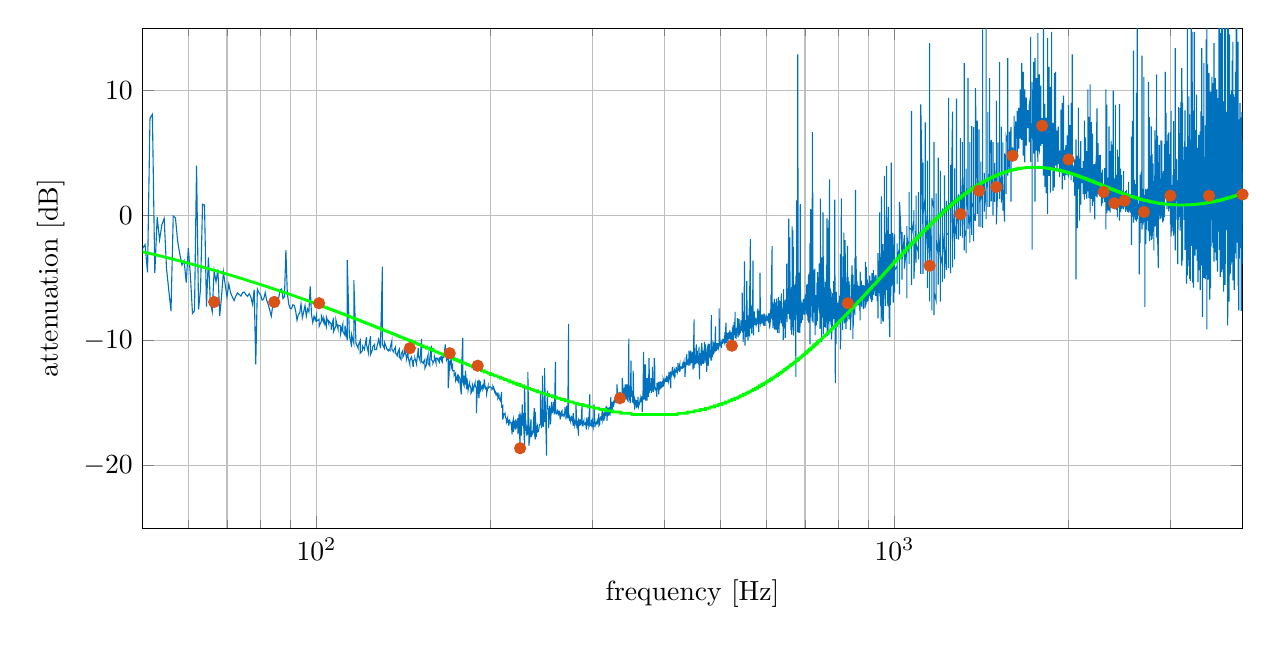
\begin{tikzpicture}

\begin{axis}[%
width=5.5in,
height=2.5in,
at={(1.011in,0.642in)},
scale only axis,
unbounded coords=jump,
xmode=log,
xmin=50,
xmax=4e+03,
xminorticks=true,
xlabel={frequency [Hz]},
xmajorgrids,
xminorgrids,
ymin=-25,
ymax=15,
ylabel={attenuation [dB]},
ymajorgrids,
axis background/.style={fill=white},
title style={font=\bfseries},
%title={Bose QuietComfort 15},
legend style={at={(0.03,0.03)},anchor=south west,legend cell align=left,align=left,draw=white!15!black}
]
\addplot [color=mycolor1,solid,forget plot]
  table[row sep=crcr]{%
0	4.97\\
0.5	0.103\\
1	6.13\\
1.5	4.74\\
2	0.0766\\
2.5	6.62\\
3	7.45\\
3.5	-3.98\\
4	-0.822\\
4.5	4.54\\
5	10.7\\
5.5	-4.93\\
6	9.98\\
6.5	3.12\\
7	3.47\\
7.5	4.59\\
8	7.15\\
8.5	0.222\\
9	-3.46\\
9.5	-5.57\\
10	2.44\\
10.5	0.889\\
11	-3.5\\
11.5	-1.02\\
12	5.3\\
12.5	-1.02\\
13	0.714\\
13.5	4.28\\
14	-0.231\\
14.5	-0.344\\
15	4.19\\
15.5	-3.09\\
16	2.21\\
16.5	-2.51\\
17	-2.59\\
17.5	2.37\\
18	1.89\\
18.5	-2.41\\
19	-1.66\\
19.5	1.48\\
20	2.28\\
20.5	-7.06\\
21	-0.409\\
21.5	-0.495\\
22	-1.27\\
22.5	3.84\\
23	-1.22\\
23.5	-3.46\\
24	-0.493\\
24.5	11.1\\
25	6.48\\
25.5	3.69\\
26	1.2\\
26.5	10.8\\
27	-3.16\\
27.5	-4.42\\
28	9.71\\
28.5	0.0166\\
29	-2.49\\
29.5	-1.36\\
30	2.56\\
30.5	5.38\\
31	-1.17\\
31.5	-3.77\\
32	8.18\\
32.5	6.21\\
33	-0.0979\\
33.5	2.15\\
34	8.81\\
34.5	-0.27\\
35	5.93\\
35.5	-0.763\\
36	-3.72\\
36.5	-5.08\\
37	-0.766\\
37.5	-1.6\\
38	-3.01\\
38.5	0.871\\
39	-4.36\\
39.5	-0.39\\
40	-0.563\\
40.5	3.2\\
41	-3.41\\
41.5	-2.51\\
42	0.756\\
42.5	-5.15\\
43	1.26\\
43.5	5.06\\
44	4.93\\
44.5	-4.47\\
45	-5.68\\
45.5	5.39\\
46	1.29\\
46.5	1.29\\
47	5.26\\
47.5	0.511\\
48	-2.78\\
48.5	5.92\\
49	-2.26\\
49.5	-3.69\\
50	-2.62\\
50.5	-2.31\\
51	-4.53\\
51.5	7.78\\
52	8.11\\
52.5	-4.58\\
53	-0.11\\
53.5	-1.93\\
54	-0.721\\
54.5	-0.22\\
55	-4.18\\
55.5	-5.94\\
56	-7.63\\
56.5	-0.0264\\
57	-0.16\\
57.5	-2.03\\
58	-3.06\\
58.5	-3.94\\
59	-3.59\\
59.5	-5.34\\
60	-2.58\\
60.5	-4.8\\
61	-7.81\\
61.5	-7.6\\
62	4.01\\
62.5	-7.51\\
63	-5.81\\
63.5	0.92\\
64	0.857\\
64.5	-7.27\\
65	-3.33\\
65.5	-6.87\\
66	-7.68\\
66.5	-4.42\\
67	-5.28\\
67.5	-4.3\\
68	-8.02\\
68.5	-6.44\\
69	-4.5\\
69.5	-5.52\\
70	-6.49\\
70.5	-5.47\\
71	-6.15\\
71.5	-6.51\\
72	-6.79\\
72.5	-6.43\\
73	-6.18\\
73.5	-6.3\\
74	-6.43\\
74.5	-6.14\\
75	-6.11\\
75.5	-6.33\\
76	-6.45\\
76.5	-6.23\\
77	-6.52\\
77.5	-7.08\\
78	-5.92\\
78.5	-11.9\\
79	-5.87\\
79.5	-6.17\\
80	-6.31\\
80.5	-6.75\\
81	-6.67\\
81.5	-6.16\\
82	-6.78\\
82.5	-7.11\\
83	-7.57\\
83.5	-8.03\\
84	-7.15\\
84.5	-6.94\\
85	-6.69\\
85.5	-6.68\\
86	-6.59\\
86.5	-5.93\\
87	-5.86\\
87.5	-6.63\\
88	-6.48\\
88.5	-2.76\\
89	-6.17\\
89.5	-7.07\\
90	-7.42\\
90.5	-7.44\\
91	-7.12\\
91.5	-7.17\\
92	-7.6\\
92.5	-8.35\\
93	-7.91\\
93.5	-7.79\\
94	-7.06\\
94.5	-8.16\\
95	-7.69\\
95.5	-7.19\\
96	-8.03\\
96.5	-7.46\\
97	-7.69\\
97.5	-5.65\\
98	-7.9\\
98.5	-8.55\\
99	-8.05\\
99.5	-8.35\\
100	-7.93\\
100	-8.44\\
101	-8.29\\
101	-8.86\\
102	-8.4\\
102	-8.04\\
103	-8.59\\
103	-8.23\\
104	-8.89\\
104	-8.11\\
105	-8.66\\
105	-8.41\\
106	-8.65\\
106	-9.12\\
107	-8.16\\
107	-9.28\\
108	-8.82\\
108	-8.33\\
109	-9.09\\
109	-8.76\\
110	-8.82\\
110	-9.48\\
111	-8.7\\
111	-9.23\\
112	-9.56\\
112	-8.79\\
113	-9.94\\
113	-3.55\\
114	-9.82\\
114	-9.49\\
115	-10.5\\
115	-9.52\\
116	-10.2\\
116	-5.16\\
117	-10.2\\
117	-10.2\\
118	-10.6\\
118	-10.4\\
119	-9.99\\
119	-11\\
120	-10.8\\
120	-10.4\\
121	-10.7\\
121	-10.7\\
122	-9.71\\
122	-10.3\\
123	-11\\
123	-10.5\\
124	-9.64\\
124	-11.1\\
125	-10.7\\
125	-10.5\\
126	-10.3\\
126	-10.7\\
127	-10.7\\
127	-10.6\\
128	-9.97\\
128	-9.76\\
129	-10.6\\
129	-10.4\\
130	-4.07\\
130	-10.3\\
131	-10.6\\
131	-10.1\\
132	-10.5\\
132	-10.6\\
133	-10.8\\
133	-10.7\\
134	-10.8\\
134	-10.6\\
135	-10\\
135	-10.7\\
136	-10.9\\
136	-10.8\\
137	-10.5\\
137	-11\\
138	-11.2\\
138	-11\\
139	-10.7\\
139	-11.3\\
140	-11.5\\
140	-11.1\\
141	-10.8\\
141	-11.3\\
142	-11\\
142	-10.6\\
143	-11.3\\
143	-11.5\\
144	-10.9\\
144	-11.3\\
145	-11.9\\
145	-11.6\\
146	-11.3\\
146	-11.3\\
147	-12.1\\
147	-11.6\\
148	-11.5\\
148	-11.4\\
149	-11.9\\
149	-11.7\\
150	-10.6\\
150	-11.2\\
151	-11.6\\
151	-11.5\\
152	-9.85\\
152	-11.7\\
153	-11.8\\
153	-11.7\\
154	-11.5\\
154	-12.2\\
155	-11.9\\
155	-11.6\\
156	-11.1\\
156	-11.8\\
157	-12\\
157	-11.4\\
158	-10.4\\
158	-11.5\\
159	-11.7\\
159	-11.8\\
160	-11.5\\
160	-11.3\\
161	-11.8\\
161	-11.4\\
162	-11.4\\
162	-11.5\\
163	-11.7\\
163	-11.4\\
164	-11.3\\
164	-11.5\\
165	-11.7\\
165	-11.3\\
166	-11.3\\
166	-11.4\\
167	-10.3\\
167	-11.2\\
168	-11.3\\
168	-11.5\\
169	-11.2\\
169	-13.8\\
170	-11.6\\
170	-11.9\\
171	-11.4\\
171	-12.2\\
172	-11.9\\
172	-12.4\\
173	-12.4\\
173	-12.8\\
174	-12.6\\
174	-13.2\\
175	-12.9\\
175	-13.1\\
176	-13.3\\
176	-12.8\\
177	-13\\
177	-13.3\\
178	-14.3\\
178	-13.1\\
179	-9.77\\
179	-13.3\\
180	-13.6\\
180	-12.8\\
181	-13.5\\
181	-12.4\\
182	-13.9\\
182	-13\\
183	-13.8\\
183	-13.9\\
184	-13.4\\
184	-13.5\\
185	-13.8\\
185	-14.2\\
186	-14\\
186	-13.5\\
187	-13.9\\
187	-13.8\\
188	-13.4\\
188	-13.5\\
189	-13.8\\
189	-15.8\\
190	-13.2\\
190	-13.5\\
191	-14.6\\
191	-13.2\\
192	-13.3\\
192	-14\\
193	-13.7\\
193	-13.8\\
194	-13.6\\
194	-13.9\\
195	-13.6\\
195	-13.1\\
196	-13.9\\
196	-13.7\\
197	-13.8\\
197	-14.2\\
198	-13.7\\
198	-13.8\\
199	-13.7\\
199	-13.7\\
200	-13.7\\
200	-13.7\\
201	-13.8\\
201	-13.9\\
202	-13.8\\
202	-13.7\\
203	-14\\
203	-13.9\\
204	-14.2\\
204	-14.1\\
205	-14.3\\
205	-14.2\\
206	-14.2\\
206	-14.6\\
207	-14.4\\
207	-14.6\\
208	-14.8\\
208	-14.8\\
209	-14.1\\
209	-15.3\\
210	-15.2\\
210	-16.3\\
211	-15.8\\
211	-15.9\\
212	-15.8\\
212	-16\\
213	-16.3\\
213	-16.5\\
214	-16.2\\
214	-16.5\\
215	-16.4\\
215	-16.8\\
216	-16.3\\
216	-16.5\\
217	-16.6\\
217	-16.5\\
218	-17.5\\
218	-16.7\\
219	-16.3\\
219	-17.3\\
220	-16.7\\
220	-16.4\\
221	-17.1\\
221	-16.3\\
222	-16.8\\
222	-16.8\\
223	-16.2\\
223	-17.5\\
224	-15.9\\
224	-16.3\\
225	-18.5\\
225	-15.9\\
226	-16.2\\
226	-17.6\\
227	-15.1\\
227	-16.8\\
228	-15.8\\
228	-16.3\\
229	-18.4\\
229	-13.6\\
230	-17.2\\
230	-16.3\\
231	-17.6\\
231	-16.8\\
232	-17.5\\
232	-12.5\\
233	-17\\
233	-18.4\\
234	-17.6\\
234	-17.2\\
235	-16.3\\
235	-17.7\\
236	-17.2\\
236	-17.5\\
237	-17.3\\
237	-17.1\\
238	-15.4\\
238	-17.2\\
239	-17.9\\
239	-15.7\\
240	-17.7\\
240	-17\\
241	-16.8\\
241	-17.3\\
242	-17.2\\
242	-17.3\\
243	-16.7\\
243	-16.8\\
244	-16.6\\
244	-14.1\\
245	-17\\
245	-16.9\\
246	-16.7\\
246	-12.8\\
247	-16.9\\
247	-15.7\\
248	-16.5\\
248	-12.2\\
249	-16.4\\
249	-15.7\\
250	-19.2\\
250	-16.2\\
251	-14\\
251	-15.4\\
252	-15.5\\
252	-17\\
253	-15.2\\
253	-15.7\\
254	-15.5\\
254	-16.7\\
255	-14.9\\
255	-15.2\\
256	-15.6\\
256	-15.8\\
257	-14.9\\
257	-14.9\\
258	-15.9\\
258	-15.8\\
259	-11.7\\
259	-15.5\\
260	-15.9\\
260	-15.8\\
261	-15.8\\
261	-15.5\\
262	-15.9\\
262	-15.9\\
263	-15.7\\
263	-15.6\\
264	-16.3\\
264	-16.2\\
265	-15.7\\
265	-15.7\\
266	-15.6\\
266	-16\\
267	-15.9\\
267	-15.9\\
268	-15.9\\
268	-16.1\\
269	-15.6\\
269	-15.3\\
270	-15.9\\
270	-16.3\\
271	-15.2\\
271	-15.7\\
272	-16.2\\
272	-16.2\\
273	-8.65\\
273	-15.9\\
274	-16.4\\
274	-16.1\\
275	-16.4\\
275	-16.2\\
276	-16.3\\
276	-16\\
277	-16.4\\
277	-16.1\\
278	-16.8\\
278	-15.8\\
279	-16.8\\
279	-16.3\\
280	-16.5\\
280	-16.7\\
281	-16.4\\
281	-14.9\\
282	-16.8\\
282	-17\\
283	-16.4\\
283	-16.8\\
284	-17.6\\
284	-16.3\\
285	-16.4\\
285	-16.8\\
286	-16.3\\
286	-16.7\\
287	-16.6\\
287	-16.5\\
288	-15\\
288	-16.8\\
289	-16.8\\
289	-16.6\\
290	-16.4\\
290	-16.6\\
291	-16.7\\
291	-16.7\\
292	-16.7\\
292	-16.5\\
293	-17.1\\
293	-16.4\\
294	-16.6\\
294	-16.5\\
295	-16.8\\
295	-16.1\\
296	-16.8\\
296	-16.7\\
297	-14.3\\
297	-16.8\\
298	-16.7\\
298	-16.7\\
299	-16.8\\
299	-16.4\\
300	-16.3\\
300	-16.6\\
301	-16.9\\
301	-16.5\\
302	-16.9\\
302	-15.1\\
303	-16.5\\
303	-16.6\\
304	-16.6\\
304	-16.7\\
305	-16.5\\
305	-16.5\\
306	-16.4\\
306	-16.7\\
307	-16.2\\
307	-16.5\\
308	-15.8\\
308	-16.8\\
309	-16.7\\
309	-16.4\\
310	-16.1\\
310	-16.1\\
311	-16.1\\
311	-16.4\\
312	-15.7\\
312	-15.5\\
313	-15.9\\
313	-16.3\\
314	-16\\
314	-16.4\\
315	-15.9\\
315	-16.2\\
316	-15.7\\
316	-16\\
317	-15.2\\
317	-16\\
318	-15.3\\
318	-16.4\\
319	-15.4\\
319	-15.9\\
320	-15.5\\
320	-16\\
321	-15.3\\
321	-15.9\\
322	-15.5\\
322	-16\\
323	-14.5\\
323	-15.4\\
324	-14.9\\
324	-15.6\\
325	-14.9\\
325	-15.4\\
326	-15.1\\
326	-15.3\\
327	-14.8\\
327	-15.1\\
328	-14.7\\
328	-14.8\\
329	-14.7\\
329	-14.8\\
330	-14.7\\
330	-15\\
331	-14.5\\
331	-13.5\\
332	-14.7\\
332	-14.6\\
333	-14.7\\
333	-14.6\\
334	-14.7\\
334	-14.4\\
335	-14.6\\
335	-14.1\\
336	-14.4\\
336	-14.4\\
337	-14.5\\
337	-14.2\\
338	-14.7\\
338	-13\\
339	-14\\
339	-14.6\\
340	-14.1\\
340	-13.9\\
341	-13.8\\
341	-14.7\\
342	-13.5\\
342	-14.6\\
343	-13.7\\
343	-14.6\\
344	-13.5\\
344	-14.7\\
345	-13.5\\
345	-14.8\\
346	-13.5\\
346	-14.9\\
347	-9.84\\
347	-14.4\\
348	-13.6\\
348	-14.8\\
349	-13.9\\
349	-15\\
350	-11.6\\
350	-13.4\\
351	-14.5\\
351	-14.3\\
352	-14\\
352	-14.9\\
353	-14.9\\
353	-12.4\\
354	-14.9\\
354	-15.1\\
355	-14.7\\
355	-15.5\\
356	-15.1\\
356	-14.8\\
357	-15\\
357	-14.8\\
358	-14.8\\
358	-15.4\\
359	-15\\
359	-15.1\\
360	-14.5\\
360	-15.3\\
361	-14.9\\
361	-15.2\\
362	-15\\
362	-15.1\\
363	-14.7\\
363	-14.6\\
364	-14.9\\
364	-14.6\\
365	-14.8\\
365	-14.5\\
366	-14.5\\
366	-15.7\\
367	-14.3\\
367	-14.7\\
368	-10.9\\
368	-14.4\\
369	-14.7\\
369	-11.9\\
370	-14\\
370	-14.3\\
371	-11.9\\
371	-14.8\\
372	-13.4\\
372	-14\\
373	-13\\
373	-14.8\\
374	-13.4\\
374	-13.2\\
375	-14.5\\
375	-12.7\\
376	-13.4\\
376	-11.4\\
377	-14.2\\
377	-13.6\\
378	-13.8\\
378	-14\\
379	-13.1\\
379	-13\\
380	-14.2\\
380	-14.1\\
381	-13.8\\
381	-12.1\\
382	-13.7\\
382	-13.8\\
383	-14.1\\
383	-14\\
384	-13.8\\
384	-11.4\\
385	-12.3\\
385	-13.7\\
386	-13.8\\
386	-13.9\\
387	-14\\
387	-13.8\\
388	-14.5\\
388	-13.4\\
389	-13.9\\
389	-13.8\\
390	-13.3\\
390	-13.7\\
391	-14.3\\
391	-14.1\\
392	-13.5\\
392	-13.3\\
393	-13.9\\
393	-13.3\\
394	-13.3\\
394	-13.4\\
395	-13.6\\
395	-13.8\\
396	-13.4\\
396	-13.3\\
397	-13.7\\
397	-13.4\\
398	-13.5\\
398	-13.1\\
399	-13.3\\
399	-13.4\\
400	-13.1\\
400	-13.3\\
401	-13.1\\
401	-13\\
402	-13.3\\
402	-13.1\\
403	-12.9\\
403	-12.9\\
404	-13\\
404	-13.3\\
405	-13\\
405	-13\\
406	-13.2\\
406	-13\\
407	-12.7\\
407	-12.5\\
408	-12.8\\
408	-12.9\\
409	-12.7\\
409	-12.7\\
410	-13.8\\
410	-12.5\\
411	-12.8\\
411	-12.8\\
412	-12.6\\
412	-12.5\\
413	-12.1\\
413	-12.5\\
414	-12.7\\
414	-12.7\\
415	-12.4\\
415	-12.6\\
416	-12.8\\
416	-12.4\\
417	-12.6\\
417	-12.4\\
418	-12.5\\
418	-12.5\\
419	-12.5\\
419	-12.1\\
420	-12.4\\
420	-12.3\\
421	-12.4\\
421	-12.5\\
422	-12.3\\
422	-11.8\\
423	-12.4\\
423	-12.2\\
424	-12.1\\
424	-12.1\\
425	-11.9\\
425	-12.5\\
426	-12.2\\
426	-12.1\\
427	-12.1\\
427	-12.1\\
428	-12.1\\
428	-12.2\\
429	-12.2\\
429	-12.1\\
430	-11.9\\
430	-11.9\\
431	-12.2\\
431	-11.9\\
432	-11.7\\
432	-11.8\\
433	-12\\
433	-11.7\\
434	-12.4\\
434	-12.9\\
435	-11.8\\
435	-12.2\\
436	-11.6\\
436	-11.4\\
437	-11.1\\
437	-11.9\\
438	-11.9\\
438	-11.7\\
439	-11.6\\
439	-11.9\\
440	-11.5\\
440	-11.7\\
441	-12\\
441	-10.8\\
442	-11.5\\
442	-11.7\\
443	-11.8\\
443	-11.1\\
444	-10.8\\
444	-11.8\\
445	-11.4\\
445	-11\\
446	-11.8\\
446	-11.2\\
447	-10.9\\
447	-11.8\\
448	-11.2\\
448	-12.3\\
449	-11.9\\
449	-10.5\\
450	-8.3\\
450	-12.2\\
451	-10.6\\
451	-11.5\\
452	-11.5\\
452	-11.4\\
453	-11.5\\
453	-11.9\\
454	-10.3\\
454	-10.6\\
455	-11.8\\
455	-11.4\\
456	-10.8\\
456	-11.8\\
457	-11.2\\
457	-11.6\\
458	-11.7\\
458	-11.9\\
459	-10.5\\
459	-11.6\\
460	-13.1\\
460	-11.4\\
461	-11\\
461	-11.2\\
462	-11.9\\
462	-11.8\\
463	-10.7\\
463	-12\\
464	-11.5\\
464	-10.2\\
465	-11.3\\
465	-11.5\\
466	-10.8\\
466	-11.8\\
467	-11.8\\
467	-10.9\\
468	-11.5\\
468	-11.6\\
469	-10.1\\
469	-11.6\\
470	-11\\
470	-11.8\\
471	-10.3\\
471	-11.3\\
472	-11.2\\
472	-11.6\\
473	-10.9\\
473	-12.5\\
474	-11.3\\
474	-10.7\\
475	-10.5\\
475	-11.4\\
476	-10.3\\
476	-12\\
477	-11.4\\
477	-10.3\\
478	-10.3\\
478	-11.1\\
479	-11.2\\
479	-10.8\\
480	-10.9\\
480	-11.2\\
481	-10.7\\
481	-11.6\\
482	-7.95\\
482	-11.6\\
483	-9.98\\
483	-10.7\\
484	-10.9\\
484	-10.5\\
485	-10.5\\
485	-11.1\\
486	-11\\
486	-10.2\\
487	-10.3\\
487	-11\\
488	-10.7\\
488	-10.6\\
489	-10.7\\
489	-10.3\\
490	-8.86\\
490	-10.5\\
491	-10.8\\
491	-10.5\\
492	-10.4\\
492	-10.8\\
493	-10.2\\
493	-10.6\\
494	-10.5\\
494	-10.7\\
495	-10.2\\
495	-10.3\\
496	-10.5\\
496	-10.4\\
497	-10.3\\
497	-7.41\\
498	-10.4\\
498	-10.2\\
499	-10.2\\
499	-10.3\\
500	-10.2\\
500	-10.4\\
501	-10.4\\
501	-9.92\\
502	-10.6\\
502	-10.3\\
503	-10.1\\
503	-10.2\\
504	-10.2\\
504	-10\\
505	-10.1\\
505	-10.1\\
506	-10.1\\
506	-9.95\\
507	-10\\
507	-10.1\\
508	-10.2\\
508	-9.85\\
509	-9.96\\
509	-9.51\\
510	-9.59\\
510	-9.37\\
511	-8.55\\
511	-9.65\\
512	-9.41\\
512	-10.2\\
513	-9.64\\
513	-9.55\\
514	-10\\
514	-9.71\\
515	-9.88\\
515	-9.4\\
516	-9.86\\
516	-9.65\\
517	-9.72\\
517	-9.31\\
518	-9.55\\
518	-9.7\\
519	-9.13\\
519	-9.41\\
520	-9.51\\
520	-9.9\\
521	-9.3\\
521	-10.2\\
522	-9.43\\
522	-9.38\\
523	-10.4\\
523	-9.64\\
524	-9.84\\
524	-8.93\\
525	-9.69\\
525	-9.44\\
526	-10.1\\
526	-8.76\\
527	-9.18\\
527	-9.27\\
528	-8.51\\
528	-9.56\\
529	-8.88\\
529	-9.5\\
530	-7.69\\
530	-9.78\\
531	-9.17\\
531	-8.98\\
532	-9.87\\
532	-9.74\\
533	-9.14\\
533	-8.97\\
534	-9.37\\
534	-9.4\\
535	-8.19\\
535	-8.91\\
536	-9.73\\
536	-9.37\\
537	-8.84\\
537	-9.29\\
538	-9.09\\
538	-8.26\\
539	-8.93\\
539	-9.57\\
540	-8.97\\
540	-8.88\\
541	-9.39\\
541	-8.95\\
542	-8.83\\
542	-8.38\\
543	-9.22\\
543	-8.91\\
544	-9.04\\
544	-8.43\\
545	-9.22\\
545	-6.16\\
546	-8.8\\
546	-9.05\\
547	-7.74\\
547	-10.1\\
548	-8.91\\
548	-8.39\\
549	-8.07\\
549	-8.73\\
550	-3.65\\
550	-8.91\\
551	-7.19\\
551	-10.4\\
552	-8.56\\
552	-8.35\\
553	-9.31\\
553	-8.62\\
554	-9.52\\
554	-9.71\\
555	-8.65\\
555	-5.23\\
556	-8.85\\
556	-8.66\\
557	-9.08\\
557	-9.5\\
558	-10\\
558	-7.98\\
559	-8.57\\
559	-9.17\\
560	-9.34\\
560	-8.85\\
561	-6.58\\
561	-9.64\\
562	-4.37\\
562	-7.18\\
563	-1.87\\
563	-6.89\\
564	-9.04\\
564	-7.22\\
565	-8.91\\
565	-8.24\\
566	-8.39\\
566	-9.43\\
567	-7.7\\
567	-7.09\\
568	-8.74\\
568	-8.43\\
569	-3.6\\
569	-7.93\\
570	-9.43\\
570	-9.57\\
571	-7.83\\
571	-8.18\\
572	-7.66\\
572	-8.73\\
573	-8.07\\
573	-8.29\\
574	-8.74\\
574	-8.4\\
575	-8.52\\
575	-8.2\\
576	-8.82\\
576	-8.78\\
577	-8.27\\
577	-8.62\\
578	-8.46\\
578	-8.4\\
579	-8.02\\
579	-7.53\\
580	-8.69\\
580	-7.41\\
581	-8.25\\
581	-8.19\\
582	-8.4\\
582	-9.32\\
583	-7.59\\
583	-8.26\\
584	-8.24\\
584	-8.32\\
585	-8.48\\
585	-4.58\\
586	-8.28\\
586	-8.56\\
587	-8.03\\
587	-8.65\\
588	-7.93\\
588	-7.96\\
589	-8.57\\
589	-8.25\\
590	-8.23\\
590	-7.87\\
591	-8.24\\
591	-8.33\\
592	-8.18\\
592	-8.31\\
593	-8.14\\
593	-8.5\\
594	-8.79\\
594	-8.05\\
595	-7.99\\
595	-8.34\\
596	-8.34\\
596	-8.28\\
597	-8.82\\
597	-8.32\\
598	-8.19\\
598	-8.2\\
599	-8.45\\
599	-8.27\\
600	-7.93\\
600	-8.05\\
601	-8.12\\
601	-8.27\\
602	-8.03\\
602	-8.4\\
603	-8.18\\
603	-8.26\\
604	-8.17\\
604	-8.13\\
605	-8.01\\
605	-7.83\\
606	-8.59\\
606	-7.96\\
607	-8.44\\
607	-7.79\\
608	-8.3\\
608	-9.03\\
609	-7.78\\
609	-8.71\\
610	-7.52\\
610	-8.51\\
611	-7.64\\
611	-6.32\\
612	-7.93\\
612	-7.55\\
613	-8.23\\
613	-4.45\\
614	-2.43\\
614	-7\\
615	-8.2\\
615	-6.93\\
616	-8.99\\
616	-7.92\\
617	-7.07\\
617	-8.46\\
618	-7.92\\
618	-8.8\\
619	-6.89\\
619	-7.9\\
620	-6.65\\
620	-9.11\\
621	-7.93\\
621	-7.06\\
622	-8.18\\
622	-7.83\\
623	-9.12\\
623	-6.95\\
624	-7.64\\
624	-7.73\\
625	-8.57\\
625	-6.64\\
626	-7.27\\
626	-9.13\\
627	-7.45\\
627	-9.37\\
628	-7.54\\
628	-7.91\\
629	-8.19\\
629	-8.1\\
630	-6.52\\
630	-7.97\\
631	-9.4\\
631	-6.76\\
632	-8.71\\
632	-7.16\\
633	-7.28\\
633	-6.85\\
634	-8.36\\
634	-6.84\\
635	-8.17\\
635	-8.26\\
636	-7.46\\
636	-8.58\\
637	-6.21\\
637	-7.61\\
638	-6.98\\
638	-8.61\\
639	-7.68\\
639	-7.94\\
640	-7.83\\
640	-8.86\\
641	-8.6\\
641	-7.45\\
642	-8.46\\
642	-9.95\\
643	-5.87\\
643	-7.1\\
644	-9.02\\
644	-7.13\\
645	-6.86\\
645	-8.6\\
646	-7.54\\
646	-8.04\\
647	-6.72\\
647	-9.77\\
648	-7.78\\
648	-8.22\\
649	-7.57\\
649	-7.98\\
650	-7.57\\
650	-6.91\\
651	-3.83\\
651	-7.78\\
652	-8.5\\
652	-7.18\\
653	-6.61\\
653	-5.81\\
654	-7.24\\
654	-6.21\\
655	-7.02\\
655	-7.86\\
656	-0.228\\
656	-1.32\\
657	-7.3\\
657	-4.38\\
658	-5.39\\
658	-8.24\\
659	-1.73\\
659	-3.61\\
660	-7.55\\
660	-8.31\\
661	-7.99\\
661	-5.88\\
662	-7.25\\
662	-9.14\\
663	-8.63\\
663	-5.99\\
664	-5.71\\
664	-9.52\\
665	-8.81\\
665	-0.857\\
666	-8.91\\
666	-7.16\\
667	-1.17\\
667	-6.43\\
668	-2.51\\
668	-5.55\\
669	-7.84\\
669	-9.59\\
670	-6.13\\
670	-6.88\\
671	-5.54\\
671	-8.35\\
672	-6.08\\
672	-6.91\\
673	-8.04\\
673	-5.46\\
674	-6.92\\
674	-5.76\\
675	-12.9\\
675	-4.81\\
676	-6.62\\
676	-7.13\\
677	-3.86\\
677	1.22\\
678	-7.57\\
678	-7.93\\
679	-5.66\\
679	-7.24\\
680	-9.32\\
680	12.9\\
681	-3.01\\
681	-8.06\\
682	-9.35\\
682	-6.28\\
683	-7.73\\
683	-4.56\\
684	-6.2\\
684	-5.84\\
685	-6.55\\
685	-7.48\\
686	-7.21\\
686	-9.38\\
687	0.933\\
687	-8.03\\
688	-5.84\\
688	-7.15\\
689	-7.67\\
689	-6.8\\
690	-8.6\\
690	-7.61\\
691	-8.38\\
691	-6.99\\
692	-7.9\\
692	-6.95\\
693	-7.32\\
693	-8.36\\
694	-7.04\\
694	-7.38\\
695	-6.71\\
695	-7.9\\
696	-6.66\\
696	-7.05\\
697	-7.89\\
697	-6.66\\
698	-7.76\\
698	-7.11\\
699	-7.93\\
699	-7.02\\
700	-7.6\\
700	-7.3\\
701	-6.29\\
701	-7.5\\
702	-6.32\\
702	-7.44\\
703	-6.82\\
703	-7.88\\
704	-7.16\\
704	-6.58\\
705	-6.99\\
705	-5.55\\
706	-6.74\\
706	-5.48\\
707	-8.01\\
707	-6.38\\
708	-7.7\\
708	-8.4\\
709	-5.54\\
709	-7.93\\
710	-4.7\\
710	-8.55\\
711	-5.13\\
711	-7.46\\
712	-8.07\\
712	-7.52\\
713	-4.58\\
713	-6.42\\
714	-10.3\\
714	-2.22\\
715	-6.51\\
715	-6.88\\
716	-8.14\\
716	0.533\\
717	-6.83\\
717	-6.33\\
718	-6.65\\
718	-7.22\\
719	-5.74\\
719	-6.55\\
720	-4.43\\
720	-8.44\\
721	6.68\\
721	-8.36\\
722	1.84\\
722	-7.8\\
723	-8.56\\
723	-7.22\\
724	-7.56\\
724	-4.34\\
725	-5.92\\
725	-7.76\\
726	-7.11\\
726	-5.81\\
727	-5.44\\
727	-6.82\\
728	-4.24\\
728	-7.57\\
729	-9.55\\
729	-6.74\\
730	-6.35\\
730	-7.92\\
731	-8.21\\
731	-8.6\\
732	-8.49\\
732	-8.78\\
733	-6.55\\
733	-7\\
734	-7.7\\
734	-5.36\\
735	-8.28\\
735	-8.41\\
736	-6.41\\
736	-4.52\\
737	-7.57\\
737	-4.97\\
738	-6.95\\
738	-7.28\\
739	-4.91\\
739	-6.08\\
740	-7.33\\
740	-7.14\\
741	-3.81\\
741	-7.8\\
742	-5.48\\
742	-5.6\\
743	-9.06\\
743	-4.19\\
744	-8.04\\
744	1.37\\
745	-7.76\\
745	-7.82\\
746	-5.14\\
746	-3.36\\
747	-8.99\\
747	-4.78\\
748	-10.1\\
748	-6.54\\
749	-7.37\\
749	-3.34\\
750	-5.55\\
750	-7.98\\
751	-5.84\\
751	-6.88\\
752	-8.15\\
752	0.258\\
753	-5.26\\
753	-9.49\\
754	-7.56\\
754	-4.45\\
755	-7.83\\
755	-5.75\\
756	-5.77\\
756	-7.71\\
757	-8.92\\
757	-6.21\\
758	-5.82\\
758	-8.83\\
759	-5.71\\
759	-5.3\\
760	-8.95\\
760	-6.86\\
761	-6.03\\
761	-8.53\\
762	-5.39\\
762	-3.93\\
763	-8.5\\
763	-8.2\\
764	-0.213\\
764	-7.47\\
765	-9.61\\
765	-2.52\\
766	-0.979\\
766	-7.76\\
767	-3.84\\
767	-5.53\\
768	-6.97\\
768	-6.33\\
769	-7.06\\
769	-6.85\\
770	-9.57\\
770	-0.372\\
771	-3.2\\
771	-8.25\\
772	2.91\\
772	-8.45\\
773	-5.76\\
773	-8.02\\
774	-5.86\\
774	-8.34\\
775	-7.5\\
775	-7.15\\
776	-8.74\\
776	-8.64\\
777	-6.06\\
777	-6.7\\
778	-9.91\\
778	-6.55\\
779	-8.15\\
779	-9.43\\
780	-6.94\\
780	-7.54\\
781	-8.83\\
781	-6.56\\
782	-6.2\\
782	-8.31\\
783	-7.25\\
783	-7.21\\
784	-8.25\\
784	-7.57\\
785	-5.24\\
785	-8.24\\
786	-8.05\\
786	-6.79\\
787	-6.74\\
787	-7.2\\
788	-3.95\\
788	1.29\\
789	-7.24\\
789	-8.7\\
790	-13.4\\
790	-9.7\\
791	-7.66\\
791	-7.07\\
792	-10.3\\
792	-8.62\\
793	-8.17\\
793	-6.1\\
794	-7.76\\
794	-7.2\\
795	-7.12\\
795	-8.39\\
796	-7.14\\
796	-8.66\\
797	-8.87\\
797	-6.99\\
798	-7.69\\
798	-7.57\\
799	-7.53\\
799	-7.55\\
800	-8.27\\
800	-7.74\\
801	-7.87\\
801	-6.84\\
802	-8.47\\
802	-8.44\\
803	-7.13\\
803	-7.9\\
804	-6.43\\
804	-8.63\\
805	-8.17\\
805	-6.31\\
806	-10.7\\
806	-3.08\\
807	-10\\
807	-6.65\\
808	-8.29\\
808	-7.5\\
809	1.39\\
809	-8.3\\
810	-4.93\\
810	-7.2\\
811	-7.9\\
811	-8.46\\
812	-7.1\\
812	-6.93\\
813	-7.97\\
813	-9.15\\
814	-5.09\\
814	-3.26\\
815	-8.22\\
815	-5.6\\
816	-8.08\\
816	-6.47\\
817	-4.21\\
817	-1.36\\
818	-8.44\\
818	-5.12\\
819	-8.07\\
819	-8.61\\
820	-5.65\\
820	-5.65\\
821	-6.58\\
821	-1.96\\
822	-4.24\\
822	-7.78\\
823	-6.7\\
823	-4.91\\
824	-9.08\\
824	-5.32\\
825	-7.91\\
825	-7.21\\
826	-8.25\\
826	-6.51\\
827	-7.58\\
827	-6.07\\
828	-8.46\\
828	-5.93\\
829	-2.41\\
829	-7.26\\
830	-7.02\\
830	-6.94\\
831	-7.83\\
831	-4.9\\
832	-6.94\\
832	-8\\
833	-6.55\\
833	-6.34\\
834	-8.29\\
834	-5.26\\
835	-5.7\\
835	-7.38\\
836	-6.98\\
836	-6.41\\
837	-8.06\\
837	-7.81\\
838	-7.78\\
838	-7.07\\
839	-9.16\\
839	-7.91\\
840	-6.58\\
840	-8.54\\
841	-7.76\\
841	-7.27\\
842	-4.76\\
842	-7.5\\
843	-5.98\\
843	-6.58\\
844	-7.14\\
844	-3.98\\
845	-4.93\\
845	-7.63\\
846	-5.67\\
846	-6.98\\
847	-7.68\\
847	-9.87\\
848	-4.75\\
848	-9\\
849	-6.09\\
849	-5.92\\
850	-7.16\\
850	-7.18\\
851	-5.54\\
851	-7.79\\
852	-6.79\\
852	-7.3\\
853	-5.48\\
853	-6.22\\
854	-7.95\\
854	-3.4\\
855	-5.45\\
855	-7\\
856	2.07\\
856	-4.01\\
857	-7.2\\
857	-4.91\\
858	-3.23\\
858	-6.42\\
859	-4.27\\
859	-5.44\\
860	-6.98\\
860	-6.68\\
861	-5.25\\
861	-6.75\\
862	-6.31\\
862	-6.76\\
863	-5.71\\
863	-6.47\\
864	-6.41\\
864	-5.54\\
865	-6.13\\
865	-6.29\\
866	-5.88\\
866	-6.71\\
867	-7.16\\
867	-6.75\\
868	-5.64\\
868	-6.97\\
869	-6.69\\
869	-5.96\\
870	-7.49\\
870	-6.52\\
871	-6.2\\
871	-6.78\\
872	-8.37\\
872	-4.48\\
873	-6.17\\
873	-7.15\\
874	-5.36\\
874	-6.06\\
875	-6.85\\
875	-6.14\\
876	-5.19\\
876	-6.76\\
877	-7.28\\
877	-6.32\\
878	-6.63\\
878	-6.67\\
879	-6.14\\
879	-6.45\\
880	-6.58\\
880	-6.35\\
881	-5.55\\
881	-6.05\\
882	-6.7\\
882	-5.77\\
883	-7.48\\
883	-6.45\\
884	-5.82\\
884	-5.71\\
885	-6.72\\
885	-5.57\\
886	-6.04\\
886	-6.72\\
887	-6.77\\
887	-5.98\\
888	-6.21\\
888	-6.35\\
889	-5.64\\
889	-7.4\\
890	-7.11\\
890	-3.7\\
891	-4.44\\
891	-5.6\\
892	-6.26\\
892	-5.04\\
893	-7.11\\
893	-5.94\\
894	-4.11\\
894	-4.76\\
895	-5.55\\
895	-6.44\\
896	-5.77\\
896	-6.91\\
897	-5.11\\
897	-5.81\\
898	-6.59\\
898	-5.51\\
899	-5.4\\
899	-5.84\\
900	-6.82\\
900	-5.96\\
901	-6.31\\
901	-6.03\\
902	-5.58\\
902	-6.62\\
903	-5.43\\
903	-6.17\\
904	-5.44\\
904	-6\\
905	-5.67\\
905	-5.32\\
906	-4.79\\
906	-6.19\\
907	-6.12\\
907	-5.54\\
908	-6.4\\
908	-6.01\\
909	-5.2\\
909	-6.52\\
910	-6.47\\
910	-5.86\\
911	-6.21\\
911	-5.92\\
912	-5.61\\
912	-5.68\\
913	-6.15\\
913	-6.92\\
914	-4.6\\
914	-5.24\\
915	-5.96\\
915	-4.83\\
916	-5.57\\
916	-6.74\\
917	-5.72\\
917	-5.4\\
918	-6.11\\
918	-6.07\\
919	-4.35\\
919	-5.89\\
920	-5.98\\
920	-5.74\\
921	-5.53\\
921	-6.33\\
922	-5.37\\
922	-5.16\\
923	-5.06\\
923	-5.3\\
924	-5.32\\
924	-5.75\\
925	-5.9\\
925	-5\\
926	-6\\
926	-5.86\\
927	-6\\
927	-5.26\\
928	-6.41\\
928	-5.5\\
929	-4.75\\
929	-5.26\\
930	-5.72\\
930	-5.1\\
931	-5.69\\
931	-5.88\\
932	-5.6\\
932	-5.62\\
933	-5.79\\
933	-6.86\\
934	-5.49\\
934	-5.74\\
935	-6.42\\
935	-5.39\\
936	-8.22\\
936	-3\\
937	-5.12\\
937	-4.81\\
938	-5.51\\
938	-4.73\\
939	-4.47\\
939	-4.86\\
940	-5.78\\
940	-5.8\\
941	-4.34\\
941	-6.2\\
942	-3.48\\
942	0.262\\
943	-6.45\\
943	-3.85\\
944	-4.43\\
944	-4.99\\
945	-5.46\\
945	-3.31\\
946	-4.92\\
946	-7.24\\
947	-6.16\\
947	-5.35\\
948	-5.36\\
948	-8.65\\
949	-4.73\\
949	1.55\\
950	-1.41\\
950	-4.82\\
951	-2.43\\
951	-5.65\\
952	-6.01\\
952	-6.14\\
953	-5.39\\
953	-6.55\\
954	-8.4\\
954	-2.28\\
955	-7.22\\
955	-2.81\\
956	-8.47\\
956	-3.56\\
957	-7.59\\
957	-5.72\\
958	-3.25\\
958	-5.7\\
959	-5.81\\
959	-3.48\\
960	-5.69\\
960	3.19\\
961	-5.88\\
961	-3.01\\
962	-2.71\\
962	-6.34\\
963	-4.66\\
963	-4.57\\
964	-7.21\\
964	-4.71\\
965	-4.36\\
965	-2.51\\
966	-2.02\\
966	-4.55\\
967	0.0639\\
967	-5.64\\
968	-5.14\\
968	-4.67\\
969	3.98\\
969	-5.96\\
970	-1.16\\
970	-4.08\\
971	-5.81\\
971	-3.99\\
972	-3.47\\
972	-7.03\\
973	-5.88\\
973	-6.35\\
974	-4.52\\
974	-7.23\\
975	-0.124\\
975	-3.16\\
976	-2.92\\
976	0.701\\
977	-2.3\\
977	-5.92\\
978	-5.68\\
978	-6.91\\
979	-8.27\\
979	-1.95\\
980	-8.89\\
980	-7.92\\
981	-9.71\\
981	-1.47\\
982	-2.32\\
982	-4.82\\
983	-7.13\\
983	-3.51\\
984	-3.36\\
984	-6.02\\
985	-4.46\\
985	-6.45\\
986	-4.05\\
986	-4.89\\
987	-5.66\\
987	4.24\\
988	-5.46\\
988	-5.6\\
989	-3.58\\
989	-5.46\\
990	-4.7\\
990	-4.67\\
991	-5.01\\
991	-4.2\\
992	-5.52\\
992	-5.08\\
993	-3.93\\
993	-1.37\\
994	-4.9\\
994	-4.92\\
995	-6.95\\
995	-3.67\\
996	-5.12\\
996	-4.18\\
997	-3.63\\
997	-5.35\\
998	-2.5\\
998	-4.81\\
999	-2.23\\
999	-4.83\\
1e+03	-1.49\\
1e+03	-4.2\\
1e+03	-5.19\\
1e+03	-2.97\\
1e+03	-4.34\\
1e+03	-6.16\\
1e+03	-2.22\\
1e+03	-5.42\\
1e+03	-4\\
1e+03	-4.28\\
1e+03	-4.37\\
1.01e+03	-4.03\\
1.01e+03	-4.75\\
1.01e+03	-3.67\\
1.01e+03	-4.14\\
1.01e+03	-4.59\\
1.01e+03	-5.47\\
1.01e+03	-3.94\\
1.01e+03	-3.76\\
1.01e+03	-4.9\\
1.01e+03	-2.64\\
1.01e+03	-2.22\\
1.01e+03	-4.16\\
1.01e+03	-4.88\\
1.01e+03	-3.06\\
1.01e+03	-2.8\\
1.01e+03	-4.72\\
1.01e+03	-2.57\\
1.01e+03	-2.87\\
1.01e+03	-3.56\\
1.01e+03	-3.45\\
1.02e+03	-2.57\\
1.02e+03	-5.63\\
1.02e+03	-3.51\\
1.02e+03	-4.22\\
1.02e+03	-3.3\\
1.02e+03	-3.96\\
1.02e+03	-3.34\\
1.02e+03	-4.97\\
1.02e+03	-3.74\\
1.02e+03	-3.41\\
1.02e+03	-2.46\\
1.02e+03	-4.22\\
1.02e+03	-2.28\\
1.02e+03	-2.38\\
1.02e+03	-6.3\\
1.02e+03	-6.28\\
1.02e+03	-0.87\\
1.02e+03	-3.04\\
1.02e+03	-4.28\\
1.02e+03	1.08\\
1.03e+03	-3\\
1.03e+03	-5.12\\
1.03e+03	-3.89\\
1.03e+03	-3.97\\
1.03e+03	-3.2\\
1.03e+03	-4.4\\
1.03e+03	-2.53\\
1.03e+03	-3.06\\
1.03e+03	-4.02\\
1.03e+03	-3.55\\
1.03e+03	-1.32\\
1.03e+03	-3.73\\
1.03e+03	-3.62\\
1.03e+03	-2.66\\
1.03e+03	-2.81\\
1.03e+03	-3.57\\
1.03e+03	-3.69\\
1.03e+03	-3.28\\
1.03e+03	-3.36\\
1.03e+03	-3.64\\
1.04e+03	-1.56\\
1.04e+03	-3.38\\
1.04e+03	-3.88\\
1.04e+03	-3.24\\
1.04e+03	-2.46\\
1.04e+03	-3.77\\
1.04e+03	-3.12\\
1.04e+03	-1.55\\
1.04e+03	-2.98\\
1.04e+03	-2.75\\
1.04e+03	-3.42\\
1.04e+03	-3.02\\
1.04e+03	-3.52\\
1.04e+03	-3.14\\
1.04e+03	-2.15\\
1.04e+03	-3.03\\
1.04e+03	-3.78\\
1.04e+03	-2.57\\
1.04e+03	-2.51\\
1.04e+03	-4.23\\
1.05e+03	-2.15\\
1.05e+03	-2.6\\
1.05e+03	-2.86\\
1.05e+03	-3.63\\
1.05e+03	-2.53\\
1.05e+03	-2.98\\
1.05e+03	-3.44\\
1.05e+03	-2.91\\
1.05e+03	-1.06\\
1.05e+03	-0.84\\
1.05e+03	-3.47\\
1.05e+03	-1.3\\
1.05e+03	-1.8\\
1.05e+03	-6.61\\
1.05e+03	-3.11\\
1.05e+03	-2.14\\
1.05e+03	-2.95\\
1.05e+03	-3.5\\
1.05e+03	-1.28\\
1.05e+03	-1.52\\
1.06e+03	-3.1\\
1.06e+03	-2.43\\
1.06e+03	-2.34\\
1.06e+03	-3.51\\
1.06e+03	-2.39\\
1.06e+03	-0.615\\
1.06e+03	-2.23\\
1.06e+03	-3\\
1.06e+03	-2.19\\
1.06e+03	-1.55\\
1.06e+03	-2.76\\
1.06e+03	-3.86\\
1.06e+03	1.88\\
1.06e+03	-2.21\\
1.06e+03	-2.99\\
1.06e+03	-0.891\\
1.06e+03	-1.16\\
1.06e+03	-2.75\\
1.06e+03	-2.91\\
1.06e+03	-0.975\\
1.07e+03	-1.12\\
1.07e+03	-3.35\\
1.07e+03	-2.56\\
1.07e+03	-0.829\\
1.07e+03	-3.23\\
1.07e+03	-3.01\\
1.07e+03	3.21\\
1.07e+03	-1.66\\
1.07e+03	-1.85\\
1.07e+03	-1.95\\
1.07e+03	8.38\\
1.07e+03	-4.02\\
1.07e+03	-1.38\\
1.07e+03	0.288\\
1.07e+03	-3.97\\
1.07e+03	-5.54\\
1.07e+03	-1.3\\
1.07e+03	0.0327\\
1.07e+03	-2.6\\
1.07e+03	-1.54\\
1.08e+03	-0.403\\
1.08e+03	-2.09\\
1.08e+03	-2.33\\
1.08e+03	-0.726\\
1.08e+03	-2.71\\
1.08e+03	-1.84\\
1.08e+03	0.451\\
1.08e+03	-1.78\\
1.08e+03	-3.08\\
1.08e+03	-3.34\\
1.08e+03	-0.749\\
1.08e+03	-2.07\\
1.08e+03	-3.85\\
1.08e+03	-2.21\\
1.08e+03	0.294\\
1.08e+03	-2.4\\
1.08e+03	-2.18\\
1.08e+03	-0.72\\
1.08e+03	-2.8\\
1.08e+03	-5.07\\
1.09e+03	-0.437\\
1.09e+03	0.141\\
1.09e+03	-2.98\\
1.09e+03	-2.66\\
1.09e+03	-0.125\\
1.09e+03	-1.6\\
1.09e+03	-3.75\\
1.09e+03	-2.64\\
1.09e+03	-1.49\\
1.09e+03	-2.77\\
1.09e+03	-2\\
1.09e+03	1.61\\
1.09e+03	-1.86\\
1.09e+03	-2.01\\
1.09e+03	0.634\\
1.09e+03	-1.29\\
1.09e+03	-3.58\\
1.09e+03	-2.15\\
1.09e+03	-1.12\\
1.09e+03	-2.3\\
1.1e+03	-2.96\\
1.1e+03	1.88\\
1.1e+03	-1.41\\
1.1e+03	-1.5\\
1.1e+03	-2.65\\
1.1e+03	-0.427\\
1.1e+03	-1.88\\
1.1e+03	-1.03\\
1.1e+03	-0.662\\
1.1e+03	0.98\\
1.1e+03	-1.9\\
1.1e+03	-1.5\\
1.1e+03	-0.646\\
1.1e+03	-1.82\\
1.1e+03	0.0652\\
1.1e+03	-3.49\\
1.1e+03	-2.69\\
1.1e+03	-1.82\\
1.1e+03	-0.765\\
1.1e+03	-1.28\\
1.11e+03	-1.91\\
1.11e+03	-0.949\\
1.11e+03	-1.34\\
1.11e+03	1.84\\
1.11e+03	-1.32\\
1.11e+03	-1.48\\
1.11e+03	-1.16\\
1.11e+03	-1.91\\
1.11e+03	0.137\\
1.11e+03	5.07\\
1.11e+03	-0.777\\
1.11e+03	-4.65\\
1.11e+03	2.11\\
1.11e+03	-2.2\\
1.11e+03	-0.914\\
1.11e+03	-2.67\\
1.11e+03	1.41\\
1.11e+03	-2.3\\
1.11e+03	-1.04\\
1.11e+03	8.9\\
1.12e+03	-1.64\\
1.12e+03	-4.32\\
1.12e+03	-0.47\\
1.12e+03	4.24\\
1.12e+03	-4.19\\
1.12e+03	0.292\\
1.12e+03	2.42\\
1.12e+03	-3.36\\
1.12e+03	-3.14\\
1.12e+03	3.24\\
1.12e+03	-2.04\\
1.12e+03	-1.4\\
1.12e+03	-1.81\\
1.12e+03	0.359\\
1.12e+03	-2.44\\
1.12e+03	2.26\\
1.12e+03	3.67\\
1.12e+03	3.66\\
1.12e+03	-4.66\\
1.12e+03	0.0683\\
1.13e+03	1.49\\
1.13e+03	0.191\\
1.13e+03	-1.3\\
1.13e+03	0.226\\
1.13e+03	-0.883\\
1.13e+03	-4.02\\
1.13e+03	-0.449\\
1.13e+03	-3.05\\
1.13e+03	1.28\\
1.13e+03	7.47\\
1.13e+03	4.73\\
1.13e+03	-3.15\\
1.13e+03	-0.577\\
1.13e+03	0.948\\
1.13e+03	-4.22\\
1.13e+03	-1.48\\
1.13e+03	-3.49\\
1.13e+03	2.75\\
1.13e+03	-3.65\\
1.13e+03	0.763\\
1.14e+03	-2.93\\
1.14e+03	1.22\\
1.14e+03	-1.98\\
1.14e+03	-1.64\\
1.14e+03	0.812\\
1.14e+03	-2.53\\
1.14e+03	-5.8\\
1.14e+03	-1.6\\
1.14e+03	0.00811\\
1.14e+03	-2.2\\
1.14e+03	-2.91\\
1.14e+03	4.4\\
1.14e+03	-2.08\\
1.14e+03	-4.3\\
1.14e+03	-4.11\\
1.14e+03	-0.111\\
1.14e+03	-4.93\\
1.14e+03	-5.57\\
1.14e+03	1.15\\
1.14e+03	0.0771\\
1.15e+03	-3.57\\
1.15e+03	6.45\\
1.15e+03	6.42\\
1.15e+03	-5.25\\
1.15e+03	2.18\\
1.15e+03	1.68\\
1.15e+03	-2.36\\
1.15e+03	1.58\\
1.15e+03	-6.85\\
1.15e+03	1.76\\
1.15e+03	-4.51\\
1.15e+03	13.8\\
1.15e+03	-3.01\\
1.15e+03	-6.37\\
1.15e+03	-3.11\\
1.15e+03	0.0866\\
1.15e+03	-3.23\\
1.15e+03	-4.52\\
1.15e+03	-1.86\\
1.15e+03	0.0215\\
1.16e+03	-4.35\\
1.16e+03	-2.63\\
1.16e+03	-2.17\\
1.16e+03	-4.3\\
1.16e+03	-4.72\\
1.16e+03	-0.946\\
1.16e+03	-4.04\\
1.16e+03	-6.57\\
1.16e+03	-4.37\\
1.16e+03	-2.03\\
1.16e+03	-5.14\\
1.16e+03	-6.16\\
1.16e+03	-5.01\\
1.16e+03	-2.72\\
1.16e+03	-7.58\\
1.16e+03	-2.3\\
1.16e+03	-1.43\\
1.16e+03	-5.23\\
1.16e+03	-5.79\\
1.16e+03	1.42\\
1.17e+03	0.551\\
1.17e+03	-6.03\\
1.17e+03	-3.63\\
1.17e+03	-1.46\\
1.17e+03	-3.48\\
1.17e+03	-6.54\\
1.17e+03	-5.78\\
1.17e+03	0.38\\
1.17e+03	-3.84\\
1.17e+03	-5.11\\
1.17e+03	-0.59\\
1.17e+03	-4.52\\
1.17e+03	-6.34\\
1.17e+03	-7.96\\
1.17e+03	-1.16\\
1.17e+03	-1.64\\
1.17e+03	-7.04\\
1.17e+03	-1.11\\
1.17e+03	5.88\\
1.17e+03	-6.11\\
1.18e+03	-6.79\\
1.18e+03	-1.49\\
1.18e+03	-3.31\\
1.18e+03	-3.91\\
1.18e+03	0.067\\
1.18e+03	0.644\\
1.18e+03	-3.38\\
1.18e+03	-4.63\\
1.18e+03	1.79\\
1.18e+03	-2.86\\
1.18e+03	-4.84\\
1.18e+03	-5.66\\
1.18e+03	-2.7\\
1.18e+03	-3.79\\
1.18e+03	-1.28\\
1.18e+03	-2.11\\
1.18e+03	-2.69\\
1.18e+03	-2.98\\
1.18e+03	-4.72\\
1.18e+03	-1.91\\
1.19e+03	-3.14\\
1.19e+03	-5.51\\
1.19e+03	-2.77\\
1.19e+03	4.65\\
1.19e+03	-3.97\\
1.19e+03	-3.64\\
1.19e+03	3.89\\
1.19e+03	-2.48\\
1.19e+03	-3.38\\
1.19e+03	-4.15\\
1.19e+03	-2.69\\
1.19e+03	-3.9\\
1.19e+03	-4.71\\
1.19e+03	-2.6\\
1.19e+03	-3.86\\
1.19e+03	-1.47\\
1.19e+03	-4.12\\
1.19e+03	-1.29\\
1.19e+03	-5.03\\
1.19e+03	-3.65\\
1.2e+03	-1.44\\
1.2e+03	3.59\\
1.2e+03	-2.1\\
1.2e+03	-3.64\\
1.2e+03	-1.6\\
1.2e+03	-4\\
1.2e+03	-2.81\\
1.2e+03	0.0333\\
1.2e+03	-3.73\\
1.2e+03	-6.88\\
1.2e+03	-3.8\\
1.2e+03	1.47\\
1.2e+03	-3.85\\
1.2e+03	-4.28\\
1.2e+03	-3.33\\
1.2e+03	-2.15\\
1.2e+03	-2.24\\
1.2e+03	-3.66\\
1.2e+03	-2.2\\
1.2e+03	-3.08\\
1.21e+03	-3.96\\
1.21e+03	-2.4\\
1.21e+03	0.578\\
1.21e+03	-5.32\\
1.21e+03	-3.61\\
1.21e+03	-2.18\\
1.21e+03	-3.33\\
1.21e+03	-3.09\\
1.21e+03	-4.18\\
1.21e+03	0.0155\\
1.21e+03	-2.55\\
1.21e+03	-2.81\\
1.21e+03	-2.11\\
1.21e+03	-4.17\\
1.21e+03	0.402\\
1.21e+03	-1.82\\
1.21e+03	-0.865\\
1.21e+03	-3.89\\
1.21e+03	-2.7\\
1.21e+03	-1.37\\
1.22e+03	-3.29\\
1.22e+03	-3.25\\
1.22e+03	-3.14\\
1.22e+03	-2.02\\
1.22e+03	-4.05\\
1.22e+03	-5.03\\
1.22e+03	-3.16\\
1.22e+03	-1.28\\
1.22e+03	-3.82\\
1.22e+03	-4.12\\
1.22e+03	3.23\\
1.22e+03	-2.7\\
1.22e+03	-2.06\\
1.22e+03	-4.78\\
1.22e+03	-2.38\\
1.22e+03	-3.09\\
1.22e+03	-2.65\\
1.22e+03	-3.94\\
1.22e+03	-1.25\\
1.22e+03	-2.3\\
1.23e+03	-4.35\\
1.23e+03	-0.848\\
1.23e+03	1.18\\
1.23e+03	-1.04\\
1.23e+03	-2.94\\
1.23e+03	-1.81\\
1.23e+03	-0.884\\
1.23e+03	-1.1\\
1.23e+03	-1.09\\
1.23e+03	-0.41\\
1.23e+03	-0.341\\
1.23e+03	-4.08\\
1.23e+03	-1.01\\
1.23e+03	-0.542\\
1.23e+03	-0.49\\
1.23e+03	-3.6\\
1.23e+03	-2.09\\
1.23e+03	-1.27\\
1.23e+03	-3.03\\
1.23e+03	-1.42\\
1.24e+03	-1.48\\
1.24e+03	-1.01\\
1.24e+03	-1.78\\
1.24e+03	-1.35\\
1.24e+03	9.43\\
1.24e+03	-2.92\\
1.24e+03	-2.31\\
1.24e+03	-1.06\\
1.24e+03	-2.34\\
1.24e+03	-3.18\\
1.24e+03	-2.7\\
1.24e+03	-4.2\\
1.24e+03	-0.185\\
1.24e+03	-2.15\\
1.24e+03	-2.64\\
1.24e+03	-0.0606\\
1.24e+03	-2.19\\
1.24e+03	-1.97\\
1.24e+03	-0.425\\
1.24e+03	0.764\\
1.25e+03	1.02\\
1.25e+03	4.04\\
1.25e+03	-1.49\\
1.25e+03	-0.365\\
1.25e+03	-2.54\\
1.25e+03	-2.68\\
1.25e+03	-0.189\\
1.25e+03	1.18\\
1.25e+03	-1.35\\
1.25e+03	2\\
1.25e+03	2.46\\
1.25e+03	-2.65\\
1.25e+03	-0.594\\
1.25e+03	-0.149\\
1.25e+03	-3.23\\
1.25e+03	-4.59\\
1.25e+03	-0.141\\
1.25e+03	-2.06\\
1.25e+03	3.9\\
1.25e+03	-2.54\\
1.26e+03	8.32\\
1.26e+03	-1.12\\
1.26e+03	-2.62\\
1.26e+03	-2.25\\
1.26e+03	1.95\\
1.26e+03	-4.13\\
1.26e+03	-1.91\\
1.26e+03	0.77\\
1.26e+03	-2.21\\
1.26e+03	0.848\\
1.26e+03	2.17\\
1.26e+03	-2.19\\
1.26e+03	-0.42\\
1.26e+03	0.597\\
1.26e+03	-3.14\\
1.26e+03	-0.413\\
1.26e+03	-2.2\\
1.26e+03	-3.9\\
1.26e+03	0.931\\
1.26e+03	-2.23\\
1.27e+03	0.46\\
1.27e+03	-0.344\\
1.27e+03	1.07\\
1.27e+03	-3.11\\
1.27e+03	0.472\\
1.27e+03	0.856\\
1.27e+03	-2.07\\
1.27e+03	-1.39\\
1.27e+03	-0.815\\
1.27e+03	-0.664\\
1.27e+03	-3.49\\
1.27e+03	-0.749\\
1.27e+03	0.37\\
1.27e+03	3.79\\
1.27e+03	-1.02\\
1.27e+03	-1.55\\
1.27e+03	1.42\\
1.27e+03	-1.93\\
1.27e+03	1.65\\
1.27e+03	-1.62\\
1.28e+03	-0.661\\
1.28e+03	-1.86\\
1.28e+03	-0.202\\
1.28e+03	2.11\\
1.28e+03	-1.32\\
1.28e+03	0.554\\
1.28e+03	-1.3\\
1.28e+03	9.36\\
1.28e+03	4.27\\
1.28e+03	-1.14\\
1.28e+03	-0.726\\
1.28e+03	-0.519\\
1.28e+03	7.21\\
1.28e+03	-1.51\\
1.28e+03	-0.85\\
1.28e+03	-0.701\\
1.28e+03	0.973\\
1.28e+03	1.09\\
1.28e+03	-1.37\\
1.28e+03	0.892\\
1.29e+03	-0.818\\
1.29e+03	0.0419\\
1.29e+03	1.7\\
1.29e+03	-0.907\\
1.29e+03	0.46\\
1.29e+03	-1.92\\
1.29e+03	0.171\\
1.29e+03	-0.864\\
1.29e+03	0.626\\
1.29e+03	-1.17\\
1.29e+03	-0.518\\
1.29e+03	1.13\\
1.29e+03	0.0967\\
1.29e+03	-0.381\\
1.29e+03	-0.643\\
1.29e+03	0.186\\
1.29e+03	-0.673\\
1.29e+03	1.4\\
1.29e+03	-0.211\\
1.29e+03	0.375\\
1.3e+03	0.182\\
1.3e+03	-0.601\\
1.3e+03	-1.61\\
1.3e+03	-1.19\\
1.3e+03	1.49\\
1.3e+03	-0.413\\
1.3e+03	0.536\\
1.3e+03	0.532\\
1.3e+03	-0.22\\
1.3e+03	2.02\\
1.3e+03	-0.127\\
1.3e+03	0.782\\
1.3e+03	-0.241\\
1.3e+03	0.501\\
1.3e+03	6.2\\
1.3e+03	0.0429\\
1.3e+03	0.405\\
1.3e+03	-0.91\\
1.3e+03	1.16\\
1.3e+03	-0.942\\
1.31e+03	3\\
1.31e+03	-0.331\\
1.31e+03	0.0592\\
1.31e+03	0.49\\
1.31e+03	-0.0393\\
1.31e+03	0.7\\
1.31e+03	-0.833\\
1.31e+03	0.334\\
1.31e+03	1.38\\
1.31e+03	4.43\\
1.31e+03	0.81\\
1.31e+03	-1.76\\
1.31e+03	2.46\\
1.31e+03	5.69\\
1.31e+03	-1.17\\
1.31e+03	0.113\\
1.31e+03	0.777\\
1.31e+03	0.984\\
1.31e+03	5.89\\
1.31e+03	-0.927\\
1.32e+03	3.52\\
1.32e+03	12.2\\
1.32e+03	-0.746\\
1.32e+03	0.0846\\
1.32e+03	-2.78\\
1.32e+03	5.45\\
1.32e+03	-0.578\\
1.32e+03	2.38\\
1.32e+03	-1.27\\
1.32e+03	2.27\\
1.32e+03	0.505\\
1.32e+03	-0.611\\
1.32e+03	0.184\\
1.32e+03	0.0357\\
1.32e+03	4.32\\
1.32e+03	-0.726\\
1.32e+03	-0.283\\
1.32e+03	0.99\\
1.32e+03	-0.164\\
1.32e+03	-1.08\\
1.33e+03	-1.7\\
1.33e+03	1.5\\
1.33e+03	0.00273\\
1.33e+03	2.07\\
1.33e+03	0.204\\
1.33e+03	0.569\\
1.33e+03	1.04\\
1.33e+03	-0.522\\
1.33e+03	0.523\\
1.33e+03	-0.586\\
1.33e+03	0.692\\
1.33e+03	-0.124\\
1.33e+03	2.71\\
1.33e+03	0.328\\
1.33e+03	3.76\\
1.33e+03	-2.99\\
1.33e+03	0.301\\
1.33e+03	0.979\\
1.33e+03	-0.916\\
1.33e+03	2.24\\
1.34e+03	0.241\\
1.34e+03	-0.0858\\
1.34e+03	-0.677\\
1.34e+03	11\\
1.34e+03	1.19\\
1.34e+03	0.0238\\
1.34e+03	0.875\\
1.34e+03	0.94\\
1.34e+03	-0.414\\
1.34e+03	0.361\\
1.34e+03	1.31\\
1.34e+03	-0.633\\
1.34e+03	1.28\\
1.34e+03	0.392\\
1.34e+03	1.56\\
1.34e+03	-0.836\\
1.34e+03	-0.987\\
1.34e+03	2.35\\
1.34e+03	-1.07\\
1.34e+03	0.13\\
1.35e+03	-0.765\\
1.35e+03	3.53\\
1.35e+03	-1.33\\
1.35e+03	0.507\\
1.35e+03	0.824\\
1.35e+03	0.79\\
1.35e+03	0.956\\
1.35e+03	-0.3\\
1.35e+03	0.427\\
1.35e+03	-0.216\\
1.35e+03	-2.15\\
1.35e+03	-0.881\\
1.35e+03	1.06\\
1.35e+03	-0.14\\
1.35e+03	2.78\\
1.35e+03	-1.22\\
1.35e+03	3.66\\
1.35e+03	5.88\\
1.35e+03	0.0436\\
1.35e+03	2.48\\
1.36e+03	-1.41\\
1.36e+03	2.41\\
1.36e+03	-0.0327\\
1.36e+03	6.8\\
1.36e+03	1.57\\
1.36e+03	-1.54\\
1.36e+03	1.95\\
1.36e+03	0.00899\\
1.36e+03	1.29\\
1.36e+03	1.05\\
1.36e+03	0.105\\
1.36e+03	7.17\\
1.36e+03	1.15\\
1.36e+03	1.43\\
1.36e+03	0.0793\\
1.36e+03	-0.836\\
1.36e+03	2\\
1.36e+03	-0.233\\
1.36e+03	0.28\\
1.36e+03	0.64\\
1.37e+03	1.03\\
1.37e+03	1.62\\
1.37e+03	-0.044\\
1.37e+03	1.79\\
1.37e+03	7.08\\
1.37e+03	1.07\\
1.37e+03	3.3\\
1.37e+03	-0.125\\
1.37e+03	1.89\\
1.37e+03	-0.172\\
1.37e+03	1.05\\
1.37e+03	2\\
1.37e+03	-2.04\\
1.37e+03	1.01\\
1.37e+03	0.758\\
1.37e+03	1.2\\
1.37e+03	2.36\\
1.37e+03	-1.47\\
1.37e+03	3.83\\
1.37e+03	-0.446\\
1.38e+03	0.204\\
1.38e+03	2.39\\
1.38e+03	-0.263\\
1.38e+03	2.65\\
1.38e+03	-0.412\\
1.38e+03	2.53\\
1.38e+03	1.96\\
1.38e+03	0.323\\
1.38e+03	1.4\\
1.38e+03	1.24\\
1.38e+03	1.58\\
1.38e+03	4.13\\
1.38e+03	0.0388\\
1.38e+03	1.8\\
1.38e+03	1.63\\
1.38e+03	0.718\\
1.38e+03	1.44\\
1.38e+03	1.78\\
1.38e+03	2.21\\
1.38e+03	10.2\\
1.39e+03	0.844\\
1.39e+03	2.18\\
1.39e+03	0.309\\
1.39e+03	1.84\\
1.39e+03	0.653\\
1.39e+03	0.411\\
1.39e+03	1.7\\
1.39e+03	0.648\\
1.39e+03	1.56\\
1.39e+03	1.78\\
1.39e+03	2.84\\
1.39e+03	1.78\\
1.39e+03	1.71\\
1.39e+03	0.814\\
1.39e+03	2.5\\
1.39e+03	7.61\\
1.39e+03	0.123\\
1.39e+03	2.2\\
1.39e+03	0.879\\
1.39e+03	2.34\\
1.4e+03	2.78\\
1.4e+03	-0.868\\
1.4e+03	2\\
1.4e+03	1.38\\
1.4e+03	3.4\\
1.4e+03	-0.269\\
1.4e+03	3.6\\
1.4e+03	1.46\\
1.4e+03	1.17\\
1.4e+03	2.02\\
1.4e+03	0.675\\
1.4e+03	6.9\\
1.4e+03	2.07\\
1.4e+03	1.36\\
1.4e+03	0.922\\
1.4e+03	2.18\\
1.4e+03	1.55\\
1.4e+03	0.889\\
1.4e+03	3.52\\
1.4e+03	0.917\\
1.41e+03	2.2\\
1.41e+03	1.18\\
1.41e+03	-0.182\\
1.41e+03	3.11\\
1.41e+03	0.598\\
1.41e+03	2.72\\
1.41e+03	-0.899\\
1.41e+03	0.388\\
1.41e+03	0.285\\
1.41e+03	1.85\\
1.41e+03	1.97\\
1.41e+03	1.15\\
1.41e+03	-0.45\\
1.41e+03	-0.85\\
1.41e+03	2.63\\
1.41e+03	0.256\\
1.41e+03	4.33\\
1.41e+03	0.903\\
1.41e+03	0.156\\
1.41e+03	2.34\\
1.42e+03	1.22\\
1.42e+03	1.75\\
1.42e+03	1.81\\
1.42e+03	3.52\\
1.42e+03	0.0361\\
1.42e+03	3\\
1.42e+03	-0.974\\
1.42e+03	14.9\\
1.42e+03	1.52\\
1.42e+03	1.68\\
1.42e+03	1.3\\
1.42e+03	2.04\\
1.42e+03	4.31\\
1.42e+03	1.82\\
1.42e+03	2.45\\
1.42e+03	1.6\\
1.42e+03	3.12\\
1.42e+03	1.07\\
1.42e+03	1.51\\
1.42e+03	2.8\\
1.43e+03	1.81\\
1.43e+03	2.29\\
1.43e+03	1.87\\
1.43e+03	2.26\\
1.43e+03	1.75\\
1.43e+03	2.99\\
1.43e+03	1.56\\
1.43e+03	1.02\\
1.43e+03	3.12\\
1.43e+03	1.53\\
1.43e+03	2.13\\
1.43e+03	2.58\\
1.43e+03	2.39\\
1.43e+03	0.33\\
1.43e+03	2.07\\
1.43e+03	1.91\\
1.43e+03	2.16\\
1.43e+03	3.43\\
1.43e+03	3.27\\
1.43e+03	2.29\\
1.44e+03	0.838\\
1.44e+03	16.8\\
1.44e+03	1.64\\
1.44e+03	2.91\\
1.44e+03	1.94\\
1.44e+03	2.53\\
1.44e+03	-0.277\\
1.44e+03	0.967\\
1.44e+03	2.61\\
1.44e+03	2.18\\
1.44e+03	1.84\\
1.44e+03	2.52\\
1.44e+03	1.91\\
1.44e+03	1.89\\
1.44e+03	3.61\\
1.44e+03	2.02\\
1.44e+03	4.68\\
1.44e+03	2.14\\
1.44e+03	2.15\\
1.44e+03	2.14\\
1.45e+03	2.87\\
1.45e+03	3.18\\
1.45e+03	0.7\\
1.45e+03	4.05\\
1.45e+03	2.1\\
1.45e+03	3.47\\
1.45e+03	2.31\\
1.45e+03	2.61\\
1.45e+03	1.23\\
1.45e+03	1.87\\
1.45e+03	3.27\\
1.45e+03	0.853\\
1.45e+03	8.29\\
1.45e+03	2.43\\
1.45e+03	6.45\\
1.45e+03	1.32\\
1.45e+03	2.3\\
1.45e+03	3.43\\
1.45e+03	2.41\\
1.45e+03	3.41\\
1.46e+03	2.78\\
1.46e+03	4.34\\
1.46e+03	2.45\\
1.46e+03	3.52\\
1.46e+03	1.9\\
1.46e+03	8.1\\
1.46e+03	10.3\\
1.46e+03	0.708\\
1.46e+03	2.89\\
1.46e+03	2.5\\
1.46e+03	2.85\\
1.46e+03	3.46\\
1.46e+03	2.2\\
1.46e+03	1.7\\
1.46e+03	3.24\\
1.46e+03	5.54\\
1.46e+03	3.42\\
1.46e+03	11\\
1.46e+03	2.24\\
1.46e+03	4.91\\
1.47e+03	6.06\\
1.47e+03	3.87\\
1.47e+03	1.63\\
1.47e+03	3.33\\
1.47e+03	1.19\\
1.47e+03	1.84\\
1.47e+03	4.63\\
1.47e+03	2.84\\
1.47e+03	2.5\\
1.47e+03	3\\
1.47e+03	1.61\\
1.47e+03	2.59\\
1.47e+03	3.36\\
1.47e+03	1.15\\
1.47e+03	3.01\\
1.47e+03	3.16\\
1.47e+03	1.87\\
1.47e+03	3.66\\
1.47e+03	4.7\\
1.47e+03	2.39\\
1.48e+03	3.14\\
1.48e+03	3.27\\
1.48e+03	1.93\\
1.48e+03	3.38\\
1.48e+03	2.62\\
1.48e+03	0.0211\\
1.48e+03	2.29\\
1.48e+03	3.52\\
1.48e+03	2.84\\
1.48e+03	5.89\\
1.48e+03	2.25\\
1.48e+03	1.98\\
1.48e+03	3.18\\
1.48e+03	3.64\\
1.48e+03	0.925\\
1.48e+03	2.54\\
1.48e+03	2.82\\
1.48e+03	2.55\\
1.48e+03	3.96\\
1.48e+03	1.99\\
1.49e+03	1.11\\
1.49e+03	4.23\\
1.49e+03	2.7\\
1.49e+03	2.53\\
1.49e+03	1.44\\
1.49e+03	3.28\\
1.49e+03	2.82\\
1.49e+03	4.15\\
1.49e+03	2\\
1.49e+03	1.83\\
1.49e+03	3.34\\
1.49e+03	2.15\\
1.49e+03	3.39\\
1.49e+03	1.55\\
1.49e+03	2.63\\
1.49e+03	2.76\\
1.49e+03	2.94\\
1.49e+03	3.93\\
1.49e+03	2.22\\
1.49e+03	3.65\\
1.5e+03	2.05\\
1.5e+03	4.46\\
1.5e+03	2.55\\
1.5e+03	2.47\\
1.5e+03	3.11\\
1.5e+03	2.01\\
1.5e+03	9.18\\
1.5e+03	2.58\\
1.5e+03	2.8\\
1.5e+03	2.26\\
1.5e+03	3\\
1.5e+03	5\\
1.5e+03	1.85\\
1.5e+03	3.18\\
1.5e+03	2.77\\
1.5e+03	2.22\\
1.5e+03	2.85\\
1.5e+03	2.9\\
1.5e+03	3.74\\
1.5e+03	-0.684\\
1.51e+03	3.05\\
1.51e+03	2.83\\
1.51e+03	3.01\\
1.51e+03	2.5\\
1.51e+03	2.45\\
1.51e+03	3.52\\
1.51e+03	3.26\\
1.51e+03	5.87\\
1.51e+03	2.32\\
1.51e+03	2.84\\
1.51e+03	3.43\\
1.51e+03	3.3\\
1.51e+03	5.24\\
1.51e+03	3.41\\
1.51e+03	4.97\\
1.51e+03	1.91\\
1.51e+03	3.94\\
1.51e+03	2.2\\
1.51e+03	2.99\\
1.51e+03	2.45\\
1.52e+03	2.56\\
1.52e+03	3.73\\
1.52e+03	1.33\\
1.52e+03	4.36\\
1.52e+03	2.68\\
1.52e+03	2.53\\
1.52e+03	12.3\\
1.52e+03	6\\
1.52e+03	3.12\\
1.52e+03	3.7\\
1.52e+03	3.44\\
1.52e+03	4.35\\
1.52e+03	3.31\\
1.52e+03	4.33\\
1.52e+03	3.32\\
1.52e+03	3.53\\
1.52e+03	4.3\\
1.52e+03	1.86\\
1.52e+03	3.99\\
1.52e+03	2.25\\
1.53e+03	3.14\\
1.53e+03	4.26\\
1.53e+03	3.34\\
1.53e+03	3.78\\
1.53e+03	3.5\\
1.53e+03	3.87\\
1.53e+03	2.96\\
1.53e+03	2.79\\
1.53e+03	3.91\\
1.53e+03	3.28\\
1.53e+03	3.54\\
1.53e+03	3.18\\
1.53e+03	3.17\\
1.53e+03	1.74\\
1.53e+03	7.13\\
1.53e+03	2.89\\
1.53e+03	2.87\\
1.53e+03	2.81\\
1.53e+03	3.71\\
1.53e+03	1.05\\
1.54e+03	3.33\\
1.54e+03	5.86\\
1.54e+03	2.9\\
1.54e+03	4.22\\
1.54e+03	2.65\\
1.54e+03	4.93\\
1.54e+03	3.32\\
1.54e+03	3.5\\
1.54e+03	4.64\\
1.54e+03	3.36\\
1.54e+03	4.08\\
1.54e+03	3.4\\
1.54e+03	4.29\\
1.54e+03	1.24\\
1.54e+03	0.405\\
1.54e+03	3.16\\
1.54e+03	3.82\\
1.54e+03	3.78\\
1.54e+03	3.3\\
1.54e+03	2.5\\
1.55e+03	-0.465\\
1.55e+03	3.8\\
1.55e+03	3.16\\
1.55e+03	4.21\\
1.55e+03	3.16\\
1.55e+03	4.28\\
1.55e+03	3.21\\
1.55e+03	1.38\\
1.55e+03	3.31\\
1.55e+03	2.89\\
1.55e+03	4.28\\
1.55e+03	2.8\\
1.55e+03	4.5\\
1.55e+03	2.13\\
1.55e+03	2.17\\
1.55e+03	4.95\\
1.55e+03	3.35\\
1.55e+03	4.19\\
1.55e+03	2.88\\
1.55e+03	4.99\\
1.56e+03	3.23\\
1.56e+03	3.73\\
1.56e+03	3.85\\
1.56e+03	3.61\\
1.56e+03	4.09\\
1.56e+03	3.64\\
1.56e+03	3.69\\
1.56e+03	3.67\\
1.56e+03	4.24\\
1.56e+03	3.86\\
1.56e+03	4.19\\
1.56e+03	3.81\\
1.56e+03	4.77\\
1.56e+03	1.75\\
1.56e+03	3.11\\
1.56e+03	4.56\\
1.56e+03	3.57\\
1.56e+03	5.09\\
1.56e+03	2.94\\
1.56e+03	6.36\\
1.57e+03	5.87\\
1.57e+03	3.41\\
1.57e+03	5.09\\
1.57e+03	3.52\\
1.57e+03	4.9\\
1.57e+03	3.21\\
1.57e+03	3.69\\
1.57e+03	3.66\\
1.57e+03	4.39\\
1.57e+03	4.13\\
1.57e+03	4.74\\
1.57e+03	4.13\\
1.57e+03	6.46\\
1.57e+03	12.6\\
1.57e+03	3.47\\
1.57e+03	5.36\\
1.57e+03	4.35\\
1.57e+03	5.53\\
1.57e+03	3.44\\
1.57e+03	3.75\\
1.58e+03	5.37\\
1.58e+03	3.76\\
1.58e+03	5.13\\
1.58e+03	4.77\\
1.58e+03	4.38\\
1.58e+03	5.81\\
1.58e+03	3.96\\
1.58e+03	6.01\\
1.58e+03	4.47\\
1.58e+03	4.8\\
1.58e+03	5.34\\
1.58e+03	4.1\\
1.58e+03	6.71\\
1.58e+03	4.18\\
1.58e+03	3.73\\
1.58e+03	5.69\\
1.58e+03	4.87\\
1.58e+03	5.11\\
1.58e+03	4.67\\
1.58e+03	4.35\\
1.59e+03	7.09\\
1.59e+03	4\\
1.59e+03	5.28\\
1.59e+03	5.36\\
1.59e+03	4.19\\
1.59e+03	5.74\\
1.59e+03	3.71\\
1.59e+03	1.13\\
1.59e+03	5.76\\
1.59e+03	4.5\\
1.59e+03	5.82\\
1.59e+03	4.52\\
1.59e+03	4.62\\
1.59e+03	6.76\\
1.59e+03	5\\
1.59e+03	4.83\\
1.59e+03	4.71\\
1.59e+03	5.13\\
1.59e+03	4.15\\
1.59e+03	4.89\\
1.6e+03	4.78\\
1.6e+03	4.9\\
1.6e+03	5.04\\
1.6e+03	4.97\\
1.6e+03	5.07\\
1.6e+03	4.5\\
1.6e+03	5.26\\
1.6e+03	4.88\\
1.6e+03	4.94\\
1.6e+03	5.07\\
1.6e+03	4.74\\
1.6e+03	5.24\\
1.6e+03	4.92\\
1.6e+03	5.18\\
1.6e+03	5.38\\
1.6e+03	5.3\\
1.6e+03	5.35\\
1.6e+03	4.68\\
1.6e+03	5.47\\
1.6e+03	5.03\\
1.61e+03	5.37\\
1.61e+03	4.86\\
1.61e+03	5.32\\
1.61e+03	5.67\\
1.61e+03	4.92\\
1.61e+03	5.86\\
1.61e+03	5.2\\
1.61e+03	5.97\\
1.61e+03	5.79\\
1.61e+03	5.7\\
1.61e+03	5.97\\
1.61e+03	4.81\\
1.61e+03	6.52\\
1.61e+03	5\\
1.61e+03	6.1\\
1.61e+03	5.16\\
1.61e+03	6.11\\
1.61e+03	6.19\\
1.61e+03	7.98\\
1.61e+03	7.3\\
1.62e+03	4.99\\
1.62e+03	5.84\\
1.62e+03	5.83\\
1.62e+03	7.47\\
1.62e+03	4.94\\
1.62e+03	6.41\\
1.62e+03	5.66\\
1.62e+03	6.02\\
1.62e+03	6.56\\
1.62e+03	7.06\\
1.62e+03	6.83\\
1.62e+03	5.41\\
1.62e+03	6.33\\
1.62e+03	5.88\\
1.62e+03	6.55\\
1.62e+03	4.74\\
1.62e+03	6.3\\
1.62e+03	6.31\\
1.62e+03	6.59\\
1.62e+03	7.54\\
1.63e+03	6.01\\
1.63e+03	7.28\\
1.63e+03	5.05\\
1.63e+03	8\\
1.63e+03	5.71\\
1.63e+03	6.81\\
1.63e+03	6.72\\
1.63e+03	6.62\\
1.63e+03	7.99\\
1.63e+03	5.52\\
1.63e+03	7.48\\
1.63e+03	5.39\\
1.63e+03	7.38\\
1.63e+03	5.85\\
1.63e+03	7.58\\
1.63e+03	6.47\\
1.63e+03	5.78\\
1.63e+03	7.37\\
1.63e+03	6.07\\
1.63e+03	8.38\\
1.64e+03	5.45\\
1.64e+03	8.63\\
1.64e+03	5.57\\
1.64e+03	7.72\\
1.64e+03	6.06\\
1.64e+03	6.65\\
1.64e+03	7.43\\
1.64e+03	6.72\\
1.64e+03	7.68\\
1.64e+03	7.13\\
1.64e+03	7.56\\
1.64e+03	5.98\\
1.64e+03	7.18\\
1.64e+03	6.66\\
1.64e+03	6.38\\
1.64e+03	7.19\\
1.64e+03	7.32\\
1.64e+03	7.7\\
1.64e+03	5.36\\
1.64e+03	7.93\\
1.65e+03	6.76\\
1.65e+03	7.09\\
1.65e+03	7.78\\
1.65e+03	6.33\\
1.65e+03	9.01\\
1.65e+03	6.17\\
1.65e+03	9.02\\
1.65e+03	6.84\\
1.65e+03	7.6\\
1.65e+03	8.28\\
1.65e+03	8.47\\
1.65e+03	7.45\\
1.65e+03	7.36\\
1.65e+03	10.1\\
1.65e+03	6.69\\
1.65e+03	8.6\\
1.65e+03	6.72\\
1.65e+03	6.85\\
1.65e+03	7.31\\
1.65e+03	8.39\\
1.66e+03	9.5\\
1.66e+03	9.16\\
1.66e+03	9.8\\
1.66e+03	7.52\\
1.66e+03	7.97\\
1.66e+03	7.56\\
1.66e+03	6.31\\
1.66e+03	8.05\\
1.66e+03	7.11\\
1.66e+03	9.43\\
1.66e+03	7.49\\
1.66e+03	9.62\\
1.66e+03	12.2\\
1.66e+03	6.93\\
1.66e+03	10.1\\
1.66e+03	6.89\\
1.66e+03	7.9\\
1.66e+03	8.79\\
1.66e+03	8.34\\
1.66e+03	6.07\\
1.67e+03	10.7\\
1.67e+03	8.2\\
1.67e+03	11.5\\
1.67e+03	9.09\\
1.67e+03	7.43\\
1.67e+03	10\\
1.67e+03	7.51\\
1.67e+03	7.14\\
1.67e+03	7.48\\
1.67e+03	11.5\\
1.67e+03	7.03\\
1.67e+03	7.92\\
1.67e+03	7.12\\
1.67e+03	7.6\\
1.67e+03	4.81\\
1.67e+03	5.24\\
1.67e+03	9.74\\
1.67e+03	11\\
1.67e+03	7.67\\
1.67e+03	5.41\\
1.68e+03	6.72\\
1.68e+03	9.41\\
1.68e+03	6.59\\
1.68e+03	8.05\\
1.68e+03	9.63\\
1.68e+03	8.75\\
1.68e+03	10.1\\
1.68e+03	7.51\\
1.68e+03	8.65\\
1.68e+03	6.33\\
1.68e+03	9.52\\
1.68e+03	5.27\\
1.68e+03	8.44\\
1.68e+03	7.12\\
1.68e+03	6.45\\
1.68e+03	8.29\\
1.68e+03	4.27\\
1.68e+03	8.94\\
1.68e+03	8.23\\
1.68e+03	9.03\\
1.69e+03	6.68\\
1.69e+03	9.33\\
1.69e+03	6.51\\
1.69e+03	7.07\\
1.69e+03	7.09\\
1.69e+03	8.82\\
1.69e+03	7.13\\
1.69e+03	5.61\\
1.69e+03	9.44\\
1.69e+03	6.87\\
1.69e+03	9.25\\
1.69e+03	7.24\\
1.69e+03	7.53\\
1.69e+03	7.82\\
1.69e+03	6.86\\
1.69e+03	7.78\\
1.69e+03	7.41\\
1.69e+03	8.13\\
1.69e+03	7.5\\
1.69e+03	7.98\\
1.7e+03	8.03\\
1.7e+03	7.62\\
1.7e+03	8.45\\
1.7e+03	7.11\\
1.7e+03	8.27\\
1.7e+03	7.03\\
1.7e+03	7.72\\
1.7e+03	7.45\\
1.7e+03	7.27\\
1.7e+03	8.37\\
1.7e+03	7.41\\
1.7e+03	7.89\\
1.7e+03	7.15\\
1.7e+03	7.5\\
1.7e+03	8.03\\
1.7e+03	7.53\\
1.7e+03	7.45\\
1.7e+03	7.01\\
1.7e+03	8.12\\
1.7e+03	7.62\\
1.71e+03	7.96\\
1.71e+03	7.53\\
1.71e+03	7.31\\
1.71e+03	7.79\\
1.71e+03	7.14\\
1.71e+03	7.77\\
1.71e+03	7.3\\
1.71e+03	7.95\\
1.71e+03	8.53\\
1.71e+03	7.26\\
1.71e+03	7.65\\
1.71e+03	8.16\\
1.71e+03	7.44\\
1.71e+03	7.33\\
1.71e+03	7.29\\
1.71e+03	8.06\\
1.71e+03	7.39\\
1.71e+03	7.54\\
1.71e+03	5.86\\
1.71e+03	8.81\\
1.72e+03	9.61\\
1.72e+03	8.6\\
1.72e+03	10.7\\
1.72e+03	7.39\\
1.72e+03	10\\
1.72e+03	14.3\\
1.72e+03	5.81\\
1.72e+03	6.23\\
1.72e+03	7.74\\
1.72e+03	8.32\\
1.72e+03	4.82\\
1.72e+03	4.31\\
1.72e+03	7.17\\
1.72e+03	6.88\\
1.72e+03	8.24\\
1.72e+03	6.68\\
1.72e+03	7.57\\
1.72e+03	7.52\\
1.72e+03	7.24\\
1.72e+03	7.39\\
1.73e+03	6.15\\
1.73e+03	7.57\\
1.73e+03	7.66\\
1.73e+03	0.729\\
1.73e+03	7.11\\
1.73e+03	6.78\\
1.73e+03	10.7\\
1.73e+03	6.67\\
1.73e+03	10.1\\
1.73e+03	7.27\\
1.73e+03	8.46\\
1.73e+03	6.06\\
1.73e+03	7.8\\
1.73e+03	8.28\\
1.73e+03	7.18\\
1.73e+03	6.69\\
1.73e+03	-2.71\\
1.73e+03	9.66\\
1.73e+03	7.51\\
1.73e+03	10.2\\
1.74e+03	5.98\\
1.74e+03	10.4\\
1.74e+03	6.87\\
1.74e+03	9.05\\
1.74e+03	6.55\\
1.74e+03	7.23\\
1.74e+03	8.24\\
1.74e+03	6.83\\
1.74e+03	10.6\\
1.74e+03	8.04\\
1.74e+03	8.83\\
1.74e+03	8.68\\
1.74e+03	6.17\\
1.74e+03	7.82\\
1.74e+03	5.89\\
1.74e+03	12.3\\
1.74e+03	4.97\\
1.74e+03	6.07\\
1.74e+03	7.03\\
1.74e+03	7.7\\
1.75e+03	6.34\\
1.75e+03	8.99\\
1.75e+03	9.48\\
1.75e+03	1.12\\
1.75e+03	6.18\\
1.75e+03	5.33\\
1.75e+03	12.6\\
1.75e+03	3.88\\
1.75e+03	8.99\\
1.75e+03	5.72\\
1.75e+03	5.48\\
1.75e+03	7.85\\
1.75e+03	5.95\\
1.75e+03	8.31\\
1.75e+03	5.91\\
1.75e+03	9.86\\
1.75e+03	5.92\\
1.75e+03	7.59\\
1.75e+03	6.88\\
1.75e+03	5.68\\
1.76e+03	7.88\\
1.76e+03	5.21\\
1.76e+03	10.6\\
1.76e+03	7.56\\
1.76e+03	8.13\\
1.76e+03	8.31\\
1.76e+03	9.7\\
1.76e+03	6.74\\
1.76e+03	6.43\\
1.76e+03	8.28\\
1.76e+03	6.29\\
1.76e+03	7.42\\
1.76e+03	5.64\\
1.76e+03	7.13\\
1.76e+03	7.86\\
1.76e+03	8.04\\
1.76e+03	7.16\\
1.76e+03	7.52\\
1.76e+03	9.22\\
1.76e+03	11\\
1.77e+03	4.31\\
1.77e+03	7.14\\
1.77e+03	14.6\\
1.77e+03	6.08\\
1.77e+03	7.62\\
1.77e+03	5.68\\
1.77e+03	7.58\\
1.77e+03	11.2\\
1.77e+03	10.8\\
1.77e+03	8.8\\
1.77e+03	7.74\\
1.77e+03	7.51\\
1.77e+03	5.86\\
1.77e+03	6.47\\
1.77e+03	5.24\\
1.77e+03	5.86\\
1.77e+03	7.68\\
1.77e+03	5.92\\
1.77e+03	4.45\\
1.77e+03	5.61\\
1.78e+03	5.2\\
1.78e+03	6.1\\
1.78e+03	5.25\\
1.78e+03	5.29\\
1.78e+03	5.76\\
1.78e+03	11.3\\
1.78e+03	6.71\\
1.78e+03	8.67\\
1.78e+03	6.08\\
1.78e+03	9.84\\
1.78e+03	7.09\\
1.78e+03	6.61\\
1.78e+03	7.27\\
1.78e+03	5.94\\
1.78e+03	7.96\\
1.78e+03	5.49\\
1.78e+03	7.43\\
1.78e+03	9.04\\
1.78e+03	6.29\\
1.78e+03	8.36\\
1.79e+03	5.59\\
1.79e+03	10.4\\
1.79e+03	8.1\\
1.79e+03	7.86\\
1.79e+03	6.35\\
1.79e+03	6.51\\
1.79e+03	6.69\\
1.79e+03	6.42\\
1.79e+03	9.83\\
1.79e+03	6.6\\
1.79e+03	6.86\\
1.79e+03	6.27\\
1.79e+03	7.01\\
1.79e+03	7.46\\
1.79e+03	5.86\\
1.79e+03	7.38\\
1.79e+03	6.75\\
1.79e+03	6.72\\
1.79e+03	6.66\\
1.79e+03	6.48\\
1.8e+03	7.19\\
1.8e+03	6.36\\
1.8e+03	7.08\\
1.8e+03	6.16\\
1.8e+03	7.16\\
1.8e+03	6.2\\
1.8e+03	6.45\\
1.8e+03	7.8\\
1.8e+03	6.51\\
1.8e+03	7.16\\
1.8e+03	6.05\\
1.8e+03	5.89\\
1.8e+03	6.92\\
1.8e+03	6.2\\
1.8e+03	7.32\\
1.8e+03	5.75\\
1.8e+03	6.68\\
1.8e+03	6.69\\
1.8e+03	6.19\\
1.8e+03	6.52\\
1.81e+03	6.11\\
1.81e+03	9.75\\
1.81e+03	6.14\\
1.81e+03	6.26\\
1.81e+03	8.25\\
1.81e+03	6\\
1.81e+03	7.01\\
1.81e+03	5.03\\
1.81e+03	8.03\\
1.81e+03	6.05\\
1.81e+03	5.81\\
1.81e+03	10.1\\
1.81e+03	5.39\\
1.81e+03	6.77\\
1.81e+03	3.21\\
1.81e+03	6.73\\
1.81e+03	19\\
nan	nan\\
1.81e+03	19\\
1.81e+03	13.1\\
1.81e+03	7.05\\
1.81e+03	4.79\\
1.82e+03	7.53\\
1.82e+03	7.51\\
1.82e+03	2.31\\
1.82e+03	7.37\\
1.82e+03	4.96\\
1.82e+03	7.79\\
1.82e+03	7.26\\
1.82e+03	6.99\\
1.82e+03	7.39\\
1.82e+03	4.34\\
1.82e+03	7.6\\
1.82e+03	5.62\\
1.82e+03	7.53\\
1.82e+03	5.89\\
1.82e+03	2.37\\
1.82e+03	6.83\\
1.82e+03	5.34\\
1.82e+03	8.95\\
1.82e+03	5.49\\
1.82e+03	7.72\\
1.83e+03	4.75\\
1.83e+03	5.69\\
1.83e+03	4.74\\
1.83e+03	3.48\\
1.83e+03	6.88\\
1.83e+03	5.2\\
1.83e+03	6.21\\
1.83e+03	3.49\\
1.83e+03	6.4\\
1.83e+03	3.65\\
1.83e+03	5\\
1.83e+03	2.47\\
1.83e+03	4.88\\
1.83e+03	3.18\\
1.83e+03	6.49\\
1.83e+03	1.79\\
1.83e+03	5.49\\
1.83e+03	6.51\\
1.83e+03	3.65\\
1.83e+03	7.84\\
1.84e+03	6.13\\
1.84e+03	0.118\\
1.84e+03	13.4\\
1.84e+03	10.3\\
1.84e+03	7.99\\
1.84e+03	13.1\\
1.84e+03	4.79\\
1.84e+03	5.84\\
1.84e+03	8.06\\
1.84e+03	4.17\\
1.84e+03	5.75\\
1.84e+03	5.48\\
1.84e+03	7.31\\
1.84e+03	14.2\\
1.84e+03	3.96\\
1.84e+03	5.31\\
1.84e+03	4.44\\
1.84e+03	11.4\\
1.84e+03	5.13\\
1.84e+03	7.75\\
1.85e+03	7.06\\
1.85e+03	5.29\\
1.85e+03	4.14\\
1.85e+03	4.76\\
1.85e+03	11.9\\
1.85e+03	7.02\\
1.85e+03	5.28\\
1.85e+03	5.26\\
1.85e+03	5.99\\
1.85e+03	7.7\\
1.85e+03	6.06\\
1.85e+03	5.56\\
1.85e+03	3.18\\
1.85e+03	7.86\\
1.85e+03	4.45\\
1.85e+03	5.87\\
1.85e+03	3.84\\
1.85e+03	5.76\\
1.85e+03	6.35\\
1.85e+03	4.59\\
1.86e+03	4.61\\
1.86e+03	7.66\\
1.86e+03	8.53\\
1.86e+03	4.48\\
1.86e+03	10.3\\
1.86e+03	5.12\\
1.86e+03	6.66\\
1.86e+03	3.35\\
1.86e+03	3.9\\
1.86e+03	4.82\\
1.86e+03	6.86\\
1.86e+03	4.61\\
1.86e+03	4.33\\
1.86e+03	6.61\\
1.86e+03	1.85\\
1.86e+03	6.87\\
1.86e+03	4.61\\
1.86e+03	5.04\\
1.86e+03	6.64\\
1.86e+03	3.55\\
1.87e+03	4.56\\
1.87e+03	4.03\\
1.87e+03	7.34\\
1.87e+03	5.38\\
1.87e+03	4.88\\
1.87e+03	4.89\\
1.87e+03	12.3\\
1.87e+03	7.98\\
1.87e+03	5.27\\
1.87e+03	4.09\\
1.87e+03	6.01\\
1.87e+03	7.14\\
1.87e+03	5.05\\
1.87e+03	5.22\\
1.87e+03	7.87\\
1.87e+03	6.95\\
1.87e+03	4.74\\
1.87e+03	3.74\\
1.87e+03	14.7\\
1.87e+03	7.07\\
1.88e+03	5.28\\
1.88e+03	4.43\\
1.88e+03	6.01\\
1.88e+03	7.42\\
1.88e+03	4.76\\
1.88e+03	4.41\\
1.88e+03	4.55\\
1.88e+03	6.27\\
1.88e+03	4.5\\
1.88e+03	1.99\\
1.88e+03	3.25\\
1.88e+03	5.68\\
1.88e+03	5.78\\
1.88e+03	4.69\\
1.88e+03	7.1\\
1.88e+03	5.26\\
1.88e+03	5.01\\
1.88e+03	4.35\\
1.88e+03	4.98\\
1.88e+03	6.35\\
1.89e+03	6.61\\
1.89e+03	2.68\\
1.89e+03	4.6\\
1.89e+03	2.27\\
1.89e+03	11.4\\
1.89e+03	4.96\\
1.89e+03	6.6\\
1.89e+03	4.5\\
1.89e+03	4.85\\
1.89e+03	4.82\\
1.89e+03	4.6\\
1.89e+03	4.6\\
1.89e+03	4.5\\
1.89e+03	7.7\\
1.89e+03	4.8\\
1.89e+03	6.86\\
1.89e+03	4.4\\
1.89e+03	4.33\\
1.89e+03	4.72\\
1.89e+03	4.47\\
1.9e+03	6.34\\
1.9e+03	4.19\\
1.9e+03	4.53\\
1.9e+03	5.3\\
1.9e+03	4.57\\
1.9e+03	11.5\\
1.9e+03	4.09\\
1.9e+03	8.09\\
1.9e+03	4.85\\
1.9e+03	5.28\\
1.9e+03	4.19\\
1.9e+03	4.74\\
1.9e+03	4.94\\
1.9e+03	4.73\\
1.9e+03	6.29\\
1.9e+03	4.15\\
1.9e+03	6.6\\
1.9e+03	4.98\\
1.9e+03	4\\
1.9e+03	7.1\\
1.91e+03	3.69\\
1.91e+03	6.32\\
1.91e+03	4.37\\
1.91e+03	4.44\\
1.91e+03	5.09\\
1.91e+03	6.33\\
1.91e+03	3.92\\
1.91e+03	4.45\\
1.91e+03	5.45\\
1.91e+03	4.86\\
1.91e+03	4.35\\
1.91e+03	6.81\\
1.91e+03	3.8\\
1.91e+03	4.74\\
1.91e+03	4.65\\
1.91e+03	4.31\\
1.91e+03	5.72\\
1.91e+03	4.88\\
1.91e+03	4.55\\
1.91e+03	4.55\\
1.92e+03	5.59\\
1.92e+03	7.12\\
1.92e+03	4.3\\
1.92e+03	5.29\\
1.92e+03	4.12\\
1.92e+03	4.91\\
1.92e+03	4.8\\
1.92e+03	5.35\\
1.92e+03	5.16\\
1.92e+03	4.75\\
1.92e+03	4.68\\
1.92e+03	4.45\\
1.92e+03	5.28\\
1.92e+03	4.41\\
1.92e+03	4.73\\
1.92e+03	6.59\\
1.92e+03	4.93\\
1.92e+03	4.56\\
1.92e+03	4.9\\
1.92e+03	4.92\\
1.93e+03	4.4\\
1.93e+03	5.22\\
1.93e+03	4.67\\
1.93e+03	4.98\\
1.93e+03	4.41\\
1.93e+03	4.29\\
1.93e+03	4.71\\
1.93e+03	4.11\\
1.93e+03	3.64\\
1.93e+03	4.19\\
1.93e+03	4.58\\
1.93e+03	4.5\\
1.93e+03	4.26\\
1.93e+03	3.9\\
1.93e+03	3.08\\
1.93e+03	4.45\\
1.93e+03	3.37\\
1.93e+03	3.7\\
1.93e+03	3.55\\
1.93e+03	4.22\\
1.94e+03	3.84\\
1.94e+03	4.41\\
1.94e+03	4.23\\
1.94e+03	4.23\\
1.94e+03	4.74\\
1.94e+03	4.28\\
1.94e+03	4.48\\
1.94e+03	4.4\\
1.94e+03	8.48\\
1.94e+03	4.44\\
1.94e+03	4.78\\
1.94e+03	4.22\\
1.94e+03	4.58\\
1.94e+03	4.17\\
1.94e+03	4.21\\
1.94e+03	4.84\\
1.94e+03	4.81\\
1.94e+03	4.41\\
1.94e+03	5.69\\
1.94e+03	4.57\\
1.95e+03	4.01\\
1.95e+03	4.33\\
1.95e+03	6.07\\
1.95e+03	3.65\\
1.95e+03	5.54\\
1.95e+03	4.71\\
1.95e+03	5.89\\
1.95e+03	4.37\\
1.95e+03	4.44\\
1.95e+03	4.39\\
1.95e+03	4.64\\
1.95e+03	2.1\\
1.95e+03	4.92\\
1.95e+03	2.84\\
1.95e+03	7.79\\
1.95e+03	2.81\\
1.95e+03	9.01\\
1.95e+03	3.59\\
1.95e+03	5.79\\
1.95e+03	3.24\\
1.96e+03	5.17\\
1.96e+03	5.79\\
1.96e+03	4.22\\
1.96e+03	3.63\\
1.96e+03	9.6\\
1.96e+03	4.7\\
1.96e+03	5.3\\
1.96e+03	4.2\\
1.96e+03	4.23\\
1.96e+03	4.66\\
1.96e+03	5.01\\
1.96e+03	5.1\\
1.96e+03	3.28\\
1.96e+03	4.4\\
1.96e+03	4.73\\
1.96e+03	3.39\\
1.96e+03	3.16\\
1.96e+03	4.6\\
1.96e+03	5.43\\
1.96e+03	4.54\\
1.97e+03	4.18\\
1.97e+03	3.89\\
1.97e+03	5.07\\
1.97e+03	5.26\\
1.97e+03	3.9\\
1.97e+03	3.46\\
1.97e+03	4.78\\
1.97e+03	4.47\\
1.97e+03	4.4\\
1.97e+03	4.01\\
1.97e+03	4.67\\
1.97e+03	4.41\\
1.97e+03	4.12\\
1.97e+03	4.43\\
1.97e+03	4.12\\
1.97e+03	4.66\\
1.97e+03	4.8\\
1.97e+03	2.85\\
1.97e+03	3.91\\
1.97e+03	4.43\\
1.98e+03	5.65\\
1.98e+03	4.9\\
1.98e+03	3.78\\
1.98e+03	4.41\\
1.98e+03	5.16\\
1.98e+03	4.17\\
1.98e+03	4\\
1.98e+03	4.65\\
1.98e+03	4.73\\
1.98e+03	4.31\\
1.98e+03	3.96\\
1.98e+03	3.99\\
1.98e+03	3.35\\
1.98e+03	4.12\\
1.98e+03	4.16\\
1.98e+03	3.25\\
1.98e+03	3.64\\
1.98e+03	5.07\\
1.98e+03	3.83\\
1.98e+03	3.43\\
1.99e+03	3.41\\
1.99e+03	4.56\\
1.99e+03	4.31\\
1.99e+03	3.31\\
1.99e+03	3.34\\
1.99e+03	4.14\\
1.99e+03	4.31\\
1.99e+03	3.86\\
1.99e+03	3.87\\
1.99e+03	4.39\\
1.99e+03	3.61\\
1.99e+03	6.43\\
1.99e+03	3.35\\
1.99e+03	4.39\\
1.99e+03	4.26\\
1.99e+03	4.02\\
1.99e+03	3.67\\
1.99e+03	5.77\\
1.99e+03	4.82\\
1.99e+03	3.46\\
2e+03	3.19\\
2e+03	3.81\\
2e+03	4.47\\
2e+03	4.91\\
2e+03	3.57\\
2e+03	4.25\\
2e+03	3.41\\
2e+03	4.66\\
};
\addplot [color=mycolor1,solid,forget plot]
  table[row sep=crcr]{%
2e+03	4.66\\
2e+03	3.68\\
2e+03	5.96\\
2e+03	4.44\\
2e+03	4.45\\
2e+03	3.21\\
2e+03	3.65\\
2e+03	4.11\\
2e+03	6.14\\
2e+03	3.68\\
2e+03	3.83\\
2e+03	8.84\\
2e+03	6.26\\
2.01e+03	3.53\\
2.01e+03	4.34\\
2.01e+03	4.07\\
2.01e+03	4.19\\
2.01e+03	4.85\\
2.01e+03	3.83\\
2.01e+03	5.28\\
2.01e+03	4.78\\
2.01e+03	3.57\\
2.01e+03	4.4\\
2.01e+03	3.68\\
2.01e+03	4.11\\
2.01e+03	3.56\\
2.01e+03	3.49\\
2.01e+03	4.56\\
2.01e+03	7.24\\
2.01e+03	4.22\\
2.01e+03	5.48\\
2.01e+03	3.91\\
2.01e+03	4.55\\
2.02e+03	6.81\\
2.02e+03	3.6\\
2.02e+03	5.15\\
2.02e+03	7.02\\
2.02e+03	5.12\\
2.02e+03	2.83\\
2.02e+03	4.05\\
2.02e+03	4.16\\
2.02e+03	6.5\\
2.02e+03	4.12\\
2.02e+03	9.02\\
2.02e+03	8.77\\
2.02e+03	3.95\\
2.02e+03	3.54\\
2.02e+03	4.22\\
2.02e+03	3.37\\
2.02e+03	5.03\\
2.02e+03	3.73\\
2.02e+03	4.9\\
2.02e+03	3.26\\
2.03e+03	4.03\\
2.03e+03	4.17\\
2.03e+03	12.9\\
2.03e+03	4.37\\
2.03e+03	5.14\\
2.03e+03	7.36\\
2.03e+03	4.54\\
2.03e+03	3.65\\
2.03e+03	3.92\\
2.03e+03	3.58\\
2.03e+03	7.59\\
2.03e+03	3.48\\
2.03e+03	3.42\\
2.03e+03	3.78\\
2.03e+03	4.6\\
2.03e+03	3.95\\
2.03e+03	6.33\\
2.03e+03	3.48\\
2.03e+03	5.62\\
2.03e+03	3.81\\
2.04e+03	3.64\\
2.04e+03	3.49\\
2.04e+03	2.74\\
2.04e+03	3.88\\
2.04e+03	3\\
2.04e+03	3.76\\
2.04e+03	2.74\\
2.04e+03	3.41\\
2.04e+03	4.01\\
2.04e+03	3.3\\
2.04e+03	2.66\\
2.04e+03	3.2\\
2.04e+03	3.22\\
2.04e+03	3.53\\
2.04e+03	3.35\\
2.04e+03	3\\
2.04e+03	2.81\\
2.04e+03	3.34\\
2.04e+03	3.25\\
2.04e+03	3.47\\
2.05e+03	2.94\\
2.05e+03	2.89\\
2.05e+03	2.95\\
2.05e+03	2.67\\
2.05e+03	3.54\\
2.05e+03	2.91\\
2.05e+03	3.6\\
2.05e+03	2.62\\
2.05e+03	2.89\\
2.05e+03	2.56\\
2.05e+03	3.11\\
2.05e+03	2.12\\
2.05e+03	3.21\\
2.05e+03	3.03\\
2.05e+03	3.51\\
2.05e+03	4.49\\
2.05e+03	2.85\\
2.05e+03	2.16\\
2.05e+03	3.83\\
2.05e+03	1.6\\
2.06e+03	3.71\\
2.06e+03	2.03\\
2.06e+03	4.44\\
2.06e+03	3.77\\
2.06e+03	3.62\\
2.06e+03	1.64\\
2.06e+03	5.32\\
2.06e+03	2.77\\
2.06e+03	4.29\\
2.06e+03	-5.1\\
2.06e+03	2.01\\
2.06e+03	6.1\\
2.06e+03	5.12\\
2.06e+03	3.71\\
2.06e+03	2.1\\
2.06e+03	4.55\\
2.06e+03	1.67\\
2.06e+03	4.05\\
2.06e+03	2.75\\
2.06e+03	4.41\\
2.07e+03	0.826\\
2.07e+03	4.78\\
2.07e+03	-0.994\\
2.07e+03	3.94\\
2.07e+03	2.92\\
2.07e+03	2.91\\
2.07e+03	3.62\\
2.07e+03	4.07\\
2.07e+03	2.84\\
2.07e+03	3.28\\
2.07e+03	2.66\\
2.07e+03	3.33\\
2.07e+03	2.69\\
2.07e+03	3.11\\
2.07e+03	1.95\\
2.07e+03	3.09\\
2.07e+03	2.79\\
2.07e+03	2.11\\
2.07e+03	2.06\\
2.07e+03	2.54\\
2.08e+03	4.15\\
2.08e+03	2.1\\
2.08e+03	2.84\\
2.08e+03	2.68\\
2.08e+03	4.12\\
2.08e+03	8.65\\
2.08e+03	2.24\\
2.08e+03	2.52\\
2.08e+03	3.02\\
2.08e+03	4.56\\
2.08e+03	2.81\\
2.08e+03	2.38\\
2.08e+03	3.28\\
2.08e+03	2.25\\
2.08e+03	3.57\\
2.08e+03	2.26\\
2.08e+03	2.8\\
2.08e+03	2.47\\
2.08e+03	3.49\\
2.08e+03	2.43\\
2.09e+03	2.17\\
2.09e+03	2.88\\
2.09e+03	3.21\\
2.09e+03	2.87\\
2.09e+03	2.43\\
2.09e+03	2.14\\
2.09e+03	3.13\\
2.09e+03	2.78\\
2.09e+03	-0.385\\
2.09e+03	2.37\\
2.09e+03	3.1\\
2.09e+03	4.56\\
2.09e+03	2.97\\
2.09e+03	2.53\\
2.09e+03	2.98\\
2.09e+03	3.12\\
2.09e+03	2.63\\
2.09e+03	2.18\\
2.09e+03	2.84\\
2.09e+03	3.16\\
2.1e+03	5.96\\
2.1e+03	2.64\\
2.1e+03	2.71\\
2.1e+03	4.33\\
2.1e+03	3.11\\
2.1e+03	2.6\\
2.1e+03	2.79\\
2.1e+03	2.92\\
2.1e+03	3.15\\
2.1e+03	0.893\\
2.1e+03	2.84\\
2.1e+03	2.97\\
2.1e+03	2.97\\
2.1e+03	2.97\\
2.1e+03	2.98\\
2.1e+03	2.76\\
2.1e+03	3.09\\
2.1e+03	3.32\\
2.1e+03	2.99\\
2.1e+03	2.54\\
2.11e+03	3.18\\
2.11e+03	3.22\\
2.11e+03	2.77\\
2.11e+03	2.71\\
2.11e+03	2.9\\
2.11e+03	3.54\\
2.11e+03	3.29\\
2.11e+03	2.77\\
2.11e+03	2.82\\
2.11e+03	3.46\\
2.11e+03	3.75\\
2.11e+03	2.78\\
2.11e+03	2.61\\
2.11e+03	3.13\\
2.11e+03	3.81\\
2.11e+03	2.76\\
2.11e+03	2.99\\
2.11e+03	3.27\\
2.11e+03	3.56\\
2.11e+03	3.28\\
2.12e+03	3.2\\
2.12e+03	2.9\\
2.12e+03	3.55\\
2.12e+03	2.05\\
2.12e+03	2.66\\
2.12e+03	3.46\\
2.12e+03	3.09\\
2.12e+03	3.02\\
2.12e+03	2.44\\
2.12e+03	2.41\\
2.12e+03	3.15\\
2.12e+03	3.7\\
2.12e+03	2.9\\
2.12e+03	1.72\\
2.12e+03	3.04\\
2.12e+03	2.98\\
2.12e+03	1.87\\
2.12e+03	2.63\\
2.12e+03	4.37\\
2.12e+03	4.25\\
2.13e+03	2.76\\
2.13e+03	2.37\\
2.13e+03	2.78\\
2.13e+03	2.86\\
2.13e+03	5.57\\
2.13e+03	2.29\\
2.13e+03	2.72\\
2.13e+03	4.29\\
2.13e+03	7.61\\
2.13e+03	2.24\\
2.13e+03	3.04\\
2.13e+03	1.28\\
2.13e+03	3.69\\
2.13e+03	2.26\\
2.13e+03	2.03\\
2.13e+03	3.78\\
2.13e+03	3.9\\
2.13e+03	1.72\\
2.13e+03	1.74\\
2.13e+03	2.73\\
2.14e+03	3.29\\
2.14e+03	5.65\\
2.14e+03	2.29\\
2.14e+03	4.19\\
2.14e+03	6.27\\
2.14e+03	2.9\\
2.14e+03	1.75\\
2.14e+03	2.78\\
2.14e+03	4.36\\
2.14e+03	2.78\\
2.14e+03	2.3\\
2.14e+03	3.13\\
2.14e+03	3.76\\
2.14e+03	3.34\\
2.14e+03	2.21\\
2.14e+03	2.88\\
2.14e+03	3.9\\
2.14e+03	4.45\\
2.14e+03	2.26\\
2.14e+03	2.71\\
2.15e+03	2.5\\
2.15e+03	5.17\\
2.15e+03	2.32\\
2.15e+03	2.08\\
2.15e+03	2.51\\
2.15e+03	2.65\\
2.15e+03	2.33\\
2.15e+03	1.89\\
2.15e+03	3.9\\
2.15e+03	2.65\\
2.15e+03	2.47\\
2.15e+03	2.12\\
2.15e+03	4.75\\
2.15e+03	2.28\\
2.15e+03	2.68\\
2.15e+03	1.37\\
2.15e+03	2.5\\
2.15e+03	3.05\\
2.15e+03	2.3\\
2.15e+03	4.3\\
2.16e+03	1.94\\
2.16e+03	3.19\\
2.16e+03	3.42\\
2.16e+03	3.24\\
2.16e+03	3.26\\
2.16e+03	2.7\\
2.16e+03	3.29\\
2.16e+03	2.59\\
2.16e+03	3.01\\
2.16e+03	3.35\\
2.16e+03	2.89\\
2.16e+03	10.1\\
2.16e+03	4.12\\
2.16e+03	2.32\\
2.16e+03	2.57\\
2.16e+03	6.78\\
2.16e+03	4.47\\
2.16e+03	3.18\\
2.16e+03	3.43\\
2.16e+03	2.56\\
2.17e+03	2.81\\
2.17e+03	3.95\\
2.17e+03	2.3\\
2.17e+03	2.99\\
2.17e+03	3.09\\
2.17e+03	7.43\\
2.17e+03	2.36\\
2.17e+03	3.94\\
2.17e+03	2.28\\
2.17e+03	2.23\\
2.17e+03	1.41\\
2.17e+03	2.32\\
2.17e+03	2.79\\
2.17e+03	7.91\\
2.17e+03	7.19\\
2.17e+03	6.89\\
2.17e+03	2.5\\
2.17e+03	7.65\\
2.17e+03	2.84\\
2.17e+03	3\\
2.18e+03	2.74\\
2.18e+03	3.38\\
2.18e+03	2.34\\
2.18e+03	4.92\\
2.18e+03	4.26\\
2.18e+03	2.02\\
2.18e+03	3.58\\
2.18e+03	10.5\\
2.18e+03	5.37\\
2.18e+03	2.45\\
2.18e+03	2.2\\
2.18e+03	2.55\\
2.18e+03	0.912\\
2.18e+03	4.66\\
2.18e+03	2.45\\
2.18e+03	0.247\\
2.18e+03	2.41\\
2.18e+03	2.21\\
2.18e+03	2.89\\
2.18e+03	1.91\\
2.19e+03	1.9\\
2.19e+03	2.36\\
2.19e+03	1.35\\
2.19e+03	3.43\\
2.19e+03	4.4\\
2.19e+03	2.68\\
2.19e+03	3.43\\
2.19e+03	3.15\\
2.19e+03	2.15\\
2.19e+03	2.6\\
2.19e+03	2.36\\
2.19e+03	4.37\\
2.19e+03	2.18\\
2.19e+03	2.52\\
2.19e+03	2.31\\
2.19e+03	2.74\\
2.19e+03	2.27\\
2.19e+03	2.65\\
2.19e+03	7.48\\
2.19e+03	2.1\\
2.2e+03	3.1\\
2.2e+03	0.797\\
2.2e+03	3.04\\
2.2e+03	1.79\\
2.2e+03	2.67\\
2.2e+03	2.83\\
2.2e+03	2.75\\
2.2e+03	6.56\\
2.2e+03	2.39\\
2.2e+03	3.2\\
2.2e+03	1.72\\
2.2e+03	2.57\\
2.2e+03	1.34\\
2.2e+03	1.61\\
2.2e+03	4.88\\
2.2e+03	1.27\\
2.2e+03	3.54\\
2.2e+03	1.85\\
2.2e+03	3.17\\
2.2e+03	2.64\\
2.21e+03	2.9\\
2.21e+03	2.26\\
2.21e+03	2.03\\
2.21e+03	2.59\\
2.21e+03	1.72\\
2.21e+03	1.24\\
2.21e+03	1.13\\
2.21e+03	2.3\\
2.21e+03	2.93\\
2.21e+03	3.49\\
2.21e+03	2.13\\
2.21e+03	2.52\\
2.21e+03	4.1\\
2.21e+03	3.84\\
2.21e+03	1.99\\
2.21e+03	2.42\\
2.21e+03	2.08\\
2.21e+03	4.08\\
2.21e+03	1.41\\
2.21e+03	2.21\\
2.22e+03	2.77\\
2.22e+03	2.42\\
2.22e+03	2.65\\
2.22e+03	1.39\\
2.22e+03	2.51\\
2.22e+03	2.75\\
2.22e+03	1.61\\
2.22e+03	1.3\\
2.22e+03	-0.285\\
2.22e+03	2.59\\
2.22e+03	2.75\\
2.22e+03	2.13\\
2.22e+03	0.694\\
2.22e+03	2.09\\
2.22e+03	4.13\\
2.22e+03	1.85\\
2.22e+03	2.6\\
2.22e+03	1.64\\
2.22e+03	2.09\\
2.22e+03	2.97\\
2.23e+03	3.1\\
2.23e+03	1.57\\
2.23e+03	2.3\\
2.23e+03	2.64\\
2.23e+03	2.61\\
2.23e+03	3.14\\
2.23e+03	2.3\\
2.23e+03	4.28\\
2.23e+03	2.79\\
2.23e+03	2.19\\
2.23e+03	1.69\\
2.23e+03	3.06\\
2.23e+03	2.71\\
2.23e+03	3\\
2.23e+03	2.3\\
2.23e+03	3.27\\
2.23e+03	2.77\\
2.23e+03	4.04\\
2.23e+03	1.8\\
2.23e+03	2.57\\
2.24e+03	8.59\\
2.24e+03	2.88\\
2.24e+03	2.71\\
2.24e+03	2.03\\
2.24e+03	2.58\\
2.24e+03	2.55\\
2.24e+03	1.98\\
2.24e+03	2.23\\
2.24e+03	3.26\\
2.24e+03	2.65\\
2.24e+03	2.59\\
2.24e+03	2.09\\
2.24e+03	7.76\\
2.24e+03	2.96\\
2.24e+03	1.91\\
2.24e+03	2.01\\
2.24e+03	2.47\\
2.24e+03	2.89\\
2.24e+03	1.47\\
2.24e+03	2.32\\
2.25e+03	2.72\\
2.25e+03	3.88\\
2.25e+03	2.64\\
2.25e+03	1.94\\
2.25e+03	3.11\\
2.25e+03	2.43\\
2.25e+03	2.38\\
2.25e+03	2.23\\
2.25e+03	3.13\\
2.25e+03	3.25\\
2.25e+03	2.17\\
2.25e+03	1.91\\
2.25e+03	2.12\\
2.25e+03	5.8\\
2.25e+03	2.38\\
2.25e+03	1.75\\
2.25e+03	1.98\\
2.25e+03	1.86\\
2.25e+03	2.39\\
2.25e+03	2.14\\
2.26e+03	4.85\\
2.26e+03	1.83\\
2.26e+03	2.48\\
2.26e+03	1.67\\
2.26e+03	2.21\\
2.26e+03	2.3\\
2.26e+03	2.65\\
2.26e+03	2.14\\
2.26e+03	1.93\\
2.26e+03	2.31\\
2.26e+03	2.99\\
2.26e+03	2.24\\
2.26e+03	2.01\\
2.26e+03	2.35\\
2.26e+03	3.08\\
2.26e+03	1.95\\
2.26e+03	2.98\\
2.26e+03	2.15\\
2.26e+03	2.12\\
2.26e+03	3.53\\
2.27e+03	2.37\\
2.27e+03	2.62\\
2.27e+03	4.87\\
2.27e+03	3.17\\
2.27e+03	2.11\\
2.27e+03	2.89\\
2.27e+03	3.04\\
2.27e+03	2.24\\
2.27e+03	2.66\\
2.27e+03	2.19\\
2.27e+03	2.22\\
2.27e+03	4.27\\
2.27e+03	2.17\\
2.27e+03	2.42\\
2.27e+03	2.85\\
2.27e+03	2.28\\
2.27e+03	1.89\\
2.27e+03	2.97\\
2.27e+03	2.33\\
2.27e+03	3.65\\
2.28e+03	2.25\\
2.28e+03	2.42\\
2.28e+03	2.89\\
2.28e+03	1.93\\
2.28e+03	2.16\\
2.28e+03	2.27\\
2.28e+03	2.19\\
2.28e+03	0.767\\
2.28e+03	1.58\\
2.28e+03	2.3\\
2.28e+03	1.89\\
2.28e+03	2.08\\
2.28e+03	1.72\\
2.28e+03	0.766\\
2.28e+03	3.43\\
2.28e+03	1.6\\
2.28e+03	2.47\\
2.28e+03	1.75\\
2.28e+03	1.58\\
2.28e+03	1.33\\
2.29e+03	1.63\\
2.29e+03	1.15\\
2.29e+03	1.76\\
2.29e+03	2.59\\
2.29e+03	1.7\\
2.29e+03	1.84\\
2.29e+03	3.05\\
2.29e+03	2.06\\
2.29e+03	3.69\\
2.29e+03	1.83\\
2.29e+03	3.53\\
2.29e+03	1.01\\
2.29e+03	2.46\\
2.29e+03	1.38\\
2.29e+03	2.27\\
2.29e+03	2\\
2.29e+03	2.07\\
2.29e+03	2.78\\
2.29e+03	1.65\\
2.29e+03	2.55\\
2.3e+03	2.49\\
2.3e+03	2.3\\
2.3e+03	2.01\\
2.3e+03	2.27\\
2.3e+03	2.2\\
2.3e+03	1.81\\
2.3e+03	2.3\\
2.3e+03	1.55\\
2.3e+03	2.18\\
2.3e+03	1.86\\
2.3e+03	2.19\\
2.3e+03	1.94\\
2.3e+03	1.58\\
2.3e+03	2.03\\
2.3e+03	1.39\\
2.3e+03	2.44\\
2.3e+03	1.63\\
2.3e+03	2.26\\
2.3e+03	2.1\\
2.3e+03	1.85\\
2.31e+03	2.14\\
2.31e+03	1.55\\
2.31e+03	2.71\\
2.31e+03	1.55\\
2.31e+03	1.5\\
2.31e+03	1.11\\
2.31e+03	1.53\\
2.31e+03	3.8\\
2.31e+03	1.45\\
2.31e+03	1.09\\
2.31e+03	1.75\\
2.31e+03	1.22\\
2.31e+03	2.32\\
2.31e+03	1.56\\
2.31e+03	1.15\\
2.31e+03	1.88\\
2.31e+03	1.32\\
2.31e+03	2.76\\
2.31e+03	1.53\\
2.31e+03	1.59\\
2.32e+03	1.66\\
2.32e+03	1.29\\
2.32e+03	1.82\\
2.32e+03	1.32\\
2.32e+03	1.21\\
2.32e+03	-1.1\\
2.32e+03	0.627\\
2.32e+03	4.08\\
2.32e+03	10.1\\
2.32e+03	2.01\\
2.32e+03	1.82\\
2.32e+03	1.93\\
2.32e+03	1.95\\
2.32e+03	3.77\\
2.32e+03	1.83\\
2.32e+03	1.91\\
2.32e+03	1.91\\
2.32e+03	1.25\\
2.32e+03	1.94\\
2.32e+03	1.59\\
2.33e+03	2.59\\
2.33e+03	4.99\\
2.33e+03	8.89\\
2.33e+03	3.18\\
2.33e+03	4.75\\
2.33e+03	2.03\\
2.33e+03	1.27\\
2.33e+03	2.45\\
2.33e+03	2.25\\
2.33e+03	1.84\\
2.33e+03	1.76\\
2.33e+03	0.203\\
2.33e+03	3.43\\
2.33e+03	1.73\\
2.33e+03	0.828\\
2.33e+03	1.13\\
2.33e+03	2.26\\
2.33e+03	1.63\\
2.33e+03	1.42\\
2.33e+03	1.59\\
2.34e+03	1.65\\
2.34e+03	1.69\\
2.34e+03	1.82\\
2.34e+03	0.429\\
2.34e+03	1.62\\
2.34e+03	2.39\\
2.34e+03	3.04\\
2.34e+03	2.97\\
2.34e+03	1.29\\
2.34e+03	2.36\\
2.34e+03	1.63\\
2.34e+03	1.5\\
2.34e+03	2.24\\
2.34e+03	1.41\\
2.34e+03	1.92\\
2.34e+03	2.48\\
2.34e+03	0.549\\
2.34e+03	1.33\\
2.34e+03	1.79\\
2.34e+03	1.72\\
2.35e+03	2.17\\
2.35e+03	1.06\\
2.35e+03	0.404\\
2.35e+03	1.9\\
2.35e+03	3.36\\
2.35e+03	2.24\\
2.35e+03	1.39\\
2.35e+03	3.12\\
2.35e+03	1.81\\
2.35e+03	2.02\\
2.35e+03	1.98\\
2.35e+03	1.35\\
2.35e+03	2.23\\
2.35e+03	1.34\\
2.35e+03	7.14\\
2.35e+03	0.483\\
2.35e+03	3.72\\
2.35e+03	2.34\\
2.35e+03	1.49\\
2.35e+03	1.5\\
2.36e+03	1.25\\
2.36e+03	2.4\\
2.36e+03	0.957\\
2.36e+03	1.18\\
2.36e+03	1.23\\
2.36e+03	2.55\\
2.36e+03	0.255\\
2.36e+03	1.29\\
2.36e+03	1.53\\
2.36e+03	5.16\\
2.36e+03	2.44\\
2.36e+03	1.02\\
2.36e+03	3.28\\
2.36e+03	1.08\\
2.36e+03	2.43\\
2.36e+03	3.37\\
2.36e+03	0.971\\
2.36e+03	1.98\\
2.36e+03	1.35\\
2.36e+03	2.34\\
2.37e+03	1.03\\
2.37e+03	1.03\\
2.37e+03	2.42\\
2.37e+03	1.95\\
2.37e+03	2.28\\
2.37e+03	1.13\\
2.37e+03	1.87\\
2.37e+03	2.05\\
2.37e+03	1.23\\
2.37e+03	1.16\\
2.37e+03	3.81\\
2.37e+03	5.99\\
2.37e+03	1.29\\
2.37e+03	1.23\\
2.37e+03	1.31\\
2.37e+03	2.69\\
2.37e+03	1.08\\
2.37e+03	1.22\\
2.37e+03	1.29\\
2.37e+03	2.98\\
2.38e+03	2.08\\
2.38e+03	1.02\\
2.38e+03	1.8\\
2.38e+03	1.15\\
2.38e+03	5.69\\
2.38e+03	1.69\\
2.38e+03	2.13\\
2.38e+03	2.31\\
2.38e+03	0.983\\
2.38e+03	4.38\\
2.38e+03	0.994\\
2.38e+03	3.11\\
2.38e+03	1.82\\
2.38e+03	1.86\\
2.38e+03	1.61\\
2.38e+03	4.47\\
2.38e+03	5.44\\
2.38e+03	4.76\\
2.38e+03	2.47\\
2.38e+03	2.01\\
2.39e+03	0.878\\
2.39e+03	4.05\\
2.39e+03	1.28\\
2.39e+03	2.67\\
2.39e+03	1.37\\
2.39e+03	2.22\\
2.39e+03	1.24\\
2.39e+03	1.37\\
2.39e+03	1.72\\
2.39e+03	1.12\\
2.39e+03	1.15\\
2.39e+03	1.47\\
2.39e+03	5.79\\
2.39e+03	10\\
2.39e+03	1.31\\
2.39e+03	1.56\\
2.39e+03	1.31\\
2.39e+03	2.21\\
2.39e+03	1.3\\
2.39e+03	1.83\\
2.4e+03	1.64\\
2.4e+03	1.41\\
2.4e+03	2.99\\
2.4e+03	1.28\\
2.4e+03	2.6\\
2.4e+03	1.48\\
2.4e+03	1.59\\
2.4e+03	1.58\\
2.4e+03	1.22\\
2.4e+03	2.06\\
2.4e+03	1.02\\
2.4e+03	2.05\\
2.4e+03	1.6\\
2.4e+03	1.89\\
2.4e+03	2.23\\
2.4e+03	1.41\\
2.4e+03	1.86\\
2.4e+03	2.13\\
2.4e+03	1.82\\
2.4e+03	1.04\\
2.41e+03	1.58\\
2.41e+03	1.92\\
2.41e+03	1.53\\
2.41e+03	1.68\\
2.41e+03	1.27\\
2.41e+03	1.89\\
2.41e+03	2.84\\
2.41e+03	1.24\\
2.41e+03	1.98\\
2.41e+03	8.87\\
2.41e+03	2.1\\
2.41e+03	1.57\\
2.41e+03	1.35\\
2.41e+03	2.13\\
2.41e+03	4.09\\
2.41e+03	1.66\\
2.41e+03	1.2\\
2.41e+03	2.44\\
2.41e+03	1.99\\
2.41e+03	1.82\\
2.42e+03	1.08\\
2.42e+03	1.3\\
2.42e+03	2.19\\
2.42e+03	2.27\\
2.42e+03	0.851\\
2.42e+03	2.56\\
2.42e+03	1.82\\
2.42e+03	1.72\\
2.42e+03	0.581\\
2.42e+03	2.36\\
2.42e+03	1.58\\
2.42e+03	1.78\\
2.42e+03	3.25\\
2.42e+03	0.53\\
2.42e+03	0.872\\
2.42e+03	2.06\\
2.42e+03	1.18\\
2.42e+03	0.468\\
2.42e+03	0.492\\
2.42e+03	3.26\\
2.43e+03	1.27\\
2.43e+03	4.53\\
2.43e+03	-0.105\\
2.43e+03	5.28\\
2.43e+03	1.62\\
2.43e+03	0.766\\
2.43e+03	1.17\\
2.43e+03	0.807\\
2.43e+03	3.02\\
2.43e+03	0.643\\
2.43e+03	2.56\\
2.43e+03	3.09\\
2.43e+03	0.74\\
2.43e+03	2.62\\
2.43e+03	3.19\\
2.43e+03	1.8\\
2.43e+03	2.73\\
2.43e+03	2.01\\
2.43e+03	2.67\\
2.43e+03	2.93\\
2.44e+03	0.863\\
2.44e+03	3.34\\
2.44e+03	3.87\\
2.44e+03	2.49\\
2.44e+03	1.7\\
2.44e+03	4.3\\
2.44e+03	2.75\\
2.44e+03	1.68\\
2.44e+03	3.86\\
2.44e+03	2.48\\
2.44e+03	2.01\\
2.44e+03	1.02\\
2.44e+03	2.25\\
2.44e+03	4.48\\
2.44e+03	2.85\\
2.44e+03	0.974\\
2.44e+03	4.72\\
2.44e+03	2.26\\
2.44e+03	2.46\\
2.44e+03	2.09\\
2.45e+03	0.359\\
2.45e+03	2.33\\
2.45e+03	5.18\\
2.45e+03	1.49\\
2.45e+03	1.83\\
2.45e+03	-0.385\\
2.45e+03	2.96\\
2.45e+03	0.592\\
2.45e+03	0.535\\
2.45e+03	0.493\\
2.45e+03	2.17\\
2.45e+03	1.04\\
2.45e+03	2.06\\
2.45e+03	8.92\\
2.45e+03	3.41\\
2.45e+03	2.37\\
2.45e+03	0.775\\
2.45e+03	2\\
2.45e+03	1.23\\
2.45e+03	2.01\\
2.46e+03	1.67\\
2.46e+03	2.25\\
2.46e+03	2.73\\
2.46e+03	1.19\\
2.46e+03	2.1\\
2.46e+03	2\\
2.46e+03	3.1\\
2.46e+03	0.884\\
2.46e+03	2.08\\
2.46e+03	3.77\\
2.46e+03	1.7\\
2.46e+03	2.42\\
2.46e+03	0.287\\
2.46e+03	1.69\\
2.46e+03	1.14\\
2.46e+03	1.29\\
2.46e+03	0.672\\
2.46e+03	1.62\\
2.46e+03	1.83\\
2.46e+03	1.42\\
2.47e+03	0.529\\
2.47e+03	1.22\\
2.47e+03	1.58\\
2.47e+03	1.26\\
2.47e+03	1.19\\
2.47e+03	2.42\\
2.47e+03	2.75\\
2.47e+03	1.42\\
2.47e+03	0.873\\
2.47e+03	2.65\\
2.47e+03	2.04\\
2.47e+03	1.09\\
2.47e+03	1.11\\
2.47e+03	2.23\\
2.47e+03	3.24\\
2.47e+03	1.33\\
2.47e+03	1.17\\
2.47e+03	1.28\\
2.47e+03	1.46\\
2.47e+03	1.49\\
2.48e+03	2.01\\
2.48e+03	1.27\\
2.48e+03	1.43\\
2.48e+03	0.584\\
2.48e+03	1.16\\
2.48e+03	1.13\\
2.48e+03	1.37\\
2.48e+03	0.934\\
2.48e+03	0.716\\
2.48e+03	1\\
2.48e+03	1.36\\
2.48e+03	0.75\\
2.48e+03	1.52\\
2.48e+03	1.04\\
2.48e+03	1.52\\
2.48e+03	1.72\\
2.48e+03	0.884\\
2.48e+03	1.1\\
2.48e+03	1.4\\
2.48e+03	1.45\\
2.49e+03	0.891\\
2.49e+03	0.85\\
2.49e+03	1.39\\
2.49e+03	0.996\\
2.49e+03	1.45\\
2.49e+03	0.759\\
2.49e+03	1.58\\
2.49e+03	1.66\\
2.49e+03	1.24\\
2.49e+03	0.557\\
2.49e+03	1.13\\
2.49e+03	2.33\\
2.49e+03	1.17\\
2.49e+03	1.14\\
2.49e+03	0.514\\
2.49e+03	3.59\\
2.49e+03	1.29\\
2.49e+03	0.947\\
2.49e+03	3.58\\
2.49e+03	0.923\\
2.5e+03	1.24\\
2.5e+03	1.02\\
2.5e+03	0.915\\
2.5e+03	0.964\\
2.5e+03	0.835\\
2.5e+03	1.36\\
2.5e+03	0.69\\
2.5e+03	0.953\\
2.5e+03	0.869\\
2.5e+03	1.15\\
2.5e+03	1.57\\
2.5e+03	0.899\\
2.5e+03	1.44\\
2.5e+03	1.02\\
2.5e+03	1.08\\
2.5e+03	1\\
2.5e+03	0.784\\
2.5e+03	1.01\\
2.5e+03	0.882\\
2.5e+03	1.15\\
2.51e+03	1\\
2.51e+03	1.39\\
2.51e+03	1.19\\
2.51e+03	1.19\\
2.51e+03	1.97\\
2.51e+03	1.17\\
2.51e+03	0.98\\
2.51e+03	0.508\\
2.51e+03	0.898\\
2.51e+03	0.876\\
2.51e+03	0.894\\
2.51e+03	0.532\\
2.51e+03	1.33\\
2.51e+03	1.34\\
2.51e+03	0.349\\
2.51e+03	0.821\\
2.51e+03	1.01\\
2.51e+03	0.93\\
2.51e+03	0.76\\
2.51e+03	0.313\\
2.52e+03	0.908\\
2.52e+03	0.824\\
2.52e+03	0.498\\
2.52e+03	0.742\\
2.52e+03	0.763\\
2.52e+03	1.13\\
2.52e+03	0.616\\
2.52e+03	0.481\\
2.52e+03	0.743\\
2.52e+03	1.08\\
2.52e+03	0.614\\
2.52e+03	1.13\\
2.52e+03	0.797\\
2.52e+03	1.13\\
2.52e+03	0.722\\
2.52e+03	0.625\\
2.52e+03	0.507\\
2.52e+03	2.06\\
2.52e+03	1.13\\
2.52e+03	0.72\\
2.53e+03	0.511\\
2.53e+03	1.25\\
2.53e+03	0.476\\
2.53e+03	1.05\\
2.53e+03	0.868\\
2.53e+03	1.24\\
2.53e+03	1.56\\
2.53e+03	0.869\\
2.53e+03	0.28\\
2.53e+03	0.442\\
2.53e+03	1.02\\
2.53e+03	0.828\\
2.53e+03	0.802\\
2.53e+03	1\\
2.53e+03	0.872\\
2.53e+03	1.06\\
2.53e+03	0.457\\
2.53e+03	0.559\\
2.53e+03	1.04\\
2.53e+03	0.812\\
2.54e+03	1.12\\
2.54e+03	0.771\\
2.54e+03	1.05\\
2.54e+03	1.1\\
2.54e+03	0.875\\
2.54e+03	0.911\\
2.54e+03	0.929\\
2.54e+03	0.674\\
2.54e+03	0.545\\
2.54e+03	0.248\\
2.54e+03	1.04\\
2.54e+03	1.02\\
2.54e+03	0.598\\
2.54e+03	2.71\\
2.54e+03	1.11\\
2.54e+03	0.928\\
2.54e+03	0.805\\
2.54e+03	0.483\\
2.54e+03	0.71\\
2.54e+03	0.849\\
2.55e+03	0.8\\
2.55e+03	0.979\\
2.55e+03	0.589\\
2.55e+03	0.874\\
2.55e+03	0.646\\
2.55e+03	0.686\\
2.55e+03	0.774\\
2.55e+03	0.549\\
2.55e+03	0.67\\
2.55e+03	0.71\\
2.55e+03	0.836\\
2.55e+03	0.551\\
2.55e+03	1.51\\
2.55e+03	0.561\\
2.55e+03	0.957\\
2.55e+03	0.567\\
2.55e+03	0.813\\
2.55e+03	0.491\\
2.55e+03	0.822\\
2.55e+03	0.531\\
2.56e+03	0.717\\
2.56e+03	0.721\\
2.56e+03	0.56\\
2.56e+03	0.582\\
2.56e+03	0.593\\
2.56e+03	1.31\\
2.56e+03	1.44\\
2.56e+03	0.797\\
2.56e+03	1.12\\
2.56e+03	1.14\\
2.56e+03	1.67\\
2.56e+03	0.904\\
2.56e+03	0.532\\
2.56e+03	1.56\\
2.56e+03	0.9\\
2.56e+03	0.321\\
2.56e+03	0.834\\
2.56e+03	1.12\\
2.56e+03	0.249\\
2.56e+03	1.01\\
2.57e+03	0.411\\
2.57e+03	0.765\\
2.57e+03	6.32\\
2.57e+03	-0.386\\
2.57e+03	0.46\\
2.57e+03	1.22\\
2.57e+03	0.738\\
2.57e+03	0.551\\
2.57e+03	6.18\\
2.57e+03	-2.34\\
2.57e+03	0.624\\
2.57e+03	0.911\\
2.57e+03	0.693\\
2.57e+03	0.787\\
2.57e+03	0.6\\
2.57e+03	1.24\\
2.57e+03	0.785\\
2.57e+03	-0.0209\\
2.57e+03	1.83\\
2.57e+03	0.911\\
2.58e+03	0.734\\
2.58e+03	0.498\\
2.58e+03	7.58\\
2.58e+03	0.798\\
2.58e+03	0.572\\
2.58e+03	0.48\\
2.58e+03	1.13\\
2.58e+03	0.97\\
2.58e+03	0.573\\
2.58e+03	0.97\\
2.58e+03	-0.071\\
2.58e+03	0.826\\
2.58e+03	0.469\\
2.58e+03	0.459\\
2.58e+03	0.852\\
2.58e+03	0.458\\
2.58e+03	0.718\\
2.58e+03	-0.031\\
2.58e+03	0.956\\
2.58e+03	0.356\\
2.59e+03	0.659\\
2.59e+03	-0.459\\
2.59e+03	0.139\\
2.59e+03	0.751\\
2.59e+03	6.34\\
2.59e+03	1.36\\
2.59e+03	13.2\\
2.59e+03	0.179\\
2.59e+03	0.807\\
2.59e+03	0.25\\
2.59e+03	0.43\\
2.59e+03	0.3\\
2.59e+03	0.94\\
2.59e+03	0.225\\
2.59e+03	1.84\\
2.59e+03	0.143\\
2.59e+03	1.27\\
2.59e+03	3.44\\
2.59e+03	-0.561\\
2.59e+03	-0.474\\
2.6e+03	0.558\\
2.6e+03	1.07\\
2.6e+03	0.564\\
2.6e+03	0.33\\
2.6e+03	1.12\\
2.6e+03	-0.00212\\
2.6e+03	0.981\\
2.6e+03	-0.0177\\
2.6e+03	0.366\\
2.6e+03	0.305\\
2.6e+03	2.86\\
2.6e+03	0.868\\
2.6e+03	-0.0659\\
2.6e+03	0.341\\
2.6e+03	0.558\\
2.6e+03	0.775\\
2.6e+03	0.0948\\
2.6e+03	0.53\\
2.6e+03	0.986\\
2.6e+03	1.37\\
2.61e+03	0.573\\
2.61e+03	-0.177\\
2.61e+03	1.35\\
2.61e+03	1.55\\
2.61e+03	0.93\\
2.61e+03	-0.273\\
2.61e+03	0.525\\
2.61e+03	1.95\\
2.61e+03	0.942\\
2.61e+03	0.0743\\
2.61e+03	1.74\\
2.61e+03	-0.341\\
2.61e+03	1.91\\
2.61e+03	0.592\\
2.61e+03	-0.0282\\
2.61e+03	1.18\\
2.61e+03	2.52\\
2.61e+03	0.376\\
2.61e+03	0.0153\\
2.61e+03	-0.0885\\
2.62e+03	0.659\\
2.62e+03	0.903\\
2.62e+03	0.0779\\
2.62e+03	0.0405\\
2.62e+03	0.68\\
2.62e+03	1.32\\
2.62e+03	8.21\\
2.62e+03	0.409\\
2.62e+03	0.338\\
2.62e+03	1.33\\
2.62e+03	0.919\\
2.62e+03	0.665\\
2.62e+03	0.447\\
2.62e+03	1.47\\
2.62e+03	9.83\\
2.62e+03	0.773\\
2.62e+03	0.178\\
2.62e+03	1.93\\
2.62e+03	4.81\\
2.62e+03	-0.456\\
2.63e+03	-0.0209\\
2.63e+03	-0.234\\
2.63e+03	0.524\\
2.63e+03	0.395\\
2.63e+03	-0.256\\
2.63e+03	0.489\\
2.63e+03	1.1\\
2.63e+03	0.0532\\
2.63e+03	0.311\\
2.63e+03	1.48\\
2.63e+03	0.991\\
2.63e+03	0.761\\
2.63e+03	-0.0858\\
2.63e+03	0.925\\
2.63e+03	0.395\\
2.63e+03	0.486\\
2.63e+03	-0.00495\\
2.63e+03	15.8\\
2.63e+03	0.269\\
2.63e+03	1.08\\
2.64e+03	0.709\\
2.64e+03	0.521\\
2.64e+03	0.0576\\
2.64e+03	0.343\\
2.64e+03	0.893\\
2.64e+03	0.726\\
2.64e+03	0.399\\
2.64e+03	0.404\\
2.64e+03	0.0708\\
2.64e+03	0.356\\
2.64e+03	0.0351\\
2.64e+03	0.385\\
2.64e+03	0.75\\
2.64e+03	0.524\\
2.64e+03	0.356\\
2.64e+03	0.368\\
2.64e+03	0.255\\
2.64e+03	0.55\\
2.64e+03	0.172\\
2.64e+03	0.256\\
2.65e+03	0.987\\
2.65e+03	0.901\\
2.65e+03	0.372\\
2.65e+03	0.18\\
2.65e+03	-4.7\\
2.65e+03	-0.204\\
2.65e+03	-0.129\\
2.65e+03	0.588\\
2.65e+03	-0.475\\
2.65e+03	1.52\\
2.65e+03	0.262\\
2.65e+03	0.422\\
2.65e+03	0.91\\
2.65e+03	0.204\\
2.65e+03	0.213\\
2.65e+03	0.822\\
2.65e+03	0.764\\
2.65e+03	0.263\\
2.65e+03	0.283\\
2.65e+03	-0.767\\
2.66e+03	-0.302\\
2.66e+03	-0.086\\
2.66e+03	0.159\\
2.66e+03	0.216\\
2.66e+03	-2.21\\
2.66e+03	0.0476\\
2.66e+03	1.04\\
2.66e+03	-0.0856\\
2.66e+03	1.01\\
2.66e+03	0.0335\\
2.66e+03	-0.856\\
2.66e+03	0.388\\
2.66e+03	0.0209\\
2.66e+03	3.24\\
2.66e+03	1.41\\
2.66e+03	-1.38\\
2.66e+03	-0.478\\
2.66e+03	-0.247\\
2.66e+03	3.27\\
2.66e+03	0.141\\
2.67e+03	0.425\\
2.67e+03	1.74\\
2.67e+03	-0.395\\
2.67e+03	0.538\\
2.67e+03	0.0261\\
2.67e+03	0.195\\
2.67e+03	-0.542\\
2.67e+03	0.537\\
2.67e+03	-0.0971\\
2.67e+03	3.52\\
2.67e+03	0.768\\
2.67e+03	3.08\\
2.67e+03	0.801\\
2.67e+03	0.0922\\
2.67e+03	-0.494\\
2.67e+03	0.721\\
2.67e+03	-0.565\\
2.67e+03	0.00116\\
2.67e+03	0.348\\
2.67e+03	0.338\\
2.68e+03	0.636\\
2.68e+03	0.19\\
2.68e+03	0.687\\
2.68e+03	1.15\\
2.68e+03	12.8\\
2.68e+03	0.188\\
2.68e+03	0.649\\
2.68e+03	0.503\\
2.68e+03	0.827\\
2.68e+03	-0.681\\
2.68e+03	2.52\\
2.68e+03	0.882\\
2.68e+03	0.963\\
2.68e+03	-0.423\\
2.68e+03	0.321\\
2.68e+03	4.32\\
2.68e+03	0.918\\
2.68e+03	-0.909\\
2.68e+03	-1.1\\
2.68e+03	1.13\\
2.69e+03	2.15\\
2.69e+03	0.127\\
2.69e+03	0.398\\
2.69e+03	0.112\\
2.69e+03	0.19\\
2.69e+03	-0.0803\\
2.69e+03	0.04\\
2.69e+03	1.37\\
2.69e+03	0.599\\
2.69e+03	0.118\\
2.69e+03	0.0726\\
2.69e+03	-0.021\\
2.69e+03	0.561\\
2.69e+03	0.172\\
2.69e+03	0.0189\\
2.69e+03	0.248\\
2.69e+03	0.322\\
2.69e+03	0.301\\
2.69e+03	0.068\\
2.69e+03	-0.714\\
2.7e+03	-0.0205\\
2.7e+03	11.1\\
2.7e+03	6.9\\
2.7e+03	-0.488\\
2.7e+03	0.518\\
2.7e+03	2.64\\
2.7e+03	-0.296\\
2.7e+03	1.13\\
2.7e+03	0.709\\
2.7e+03	0.0364\\
2.7e+03	0.264\\
2.7e+03	0.0881\\
2.7e+03	-0.0591\\
2.7e+03	1.06\\
2.7e+03	0.166\\
2.7e+03	0.446\\
2.7e+03	2.44\\
2.7e+03	0.824\\
2.7e+03	0.82\\
2.7e+03	1.78\\
2.71e+03	-0.476\\
2.71e+03	0.201\\
2.71e+03	0.977\\
2.71e+03	0.837\\
2.71e+03	-0.16\\
2.71e+03	-7.29\\
2.71e+03	-0.185\\
2.71e+03	0.98\\
2.71e+03	0.0871\\
2.71e+03	1.11\\
2.71e+03	-0.204\\
2.71e+03	0.0234\\
2.71e+03	0.992\\
2.71e+03	-0.0221\\
2.71e+03	-0.871\\
2.71e+03	0.139\\
2.71e+03	0.546\\
2.71e+03	1.66\\
2.71e+03	-0.129\\
2.71e+03	0.114\\
2.72e+03	-0.13\\
2.72e+03	-0.716\\
2.72e+03	0.0473\\
2.72e+03	0.13\\
2.72e+03	0.0557\\
2.72e+03	0.199\\
2.72e+03	-2.28\\
2.72e+03	-0.155\\
2.72e+03	2.14\\
2.72e+03	1.02\\
2.72e+03	1.43\\
2.72e+03	-0.273\\
2.72e+03	1.3\\
2.72e+03	0.674\\
2.72e+03	1.07\\
2.72e+03	-0.541\\
2.72e+03	1.07\\
2.72e+03	2.13\\
2.72e+03	0.96\\
2.72e+03	-0.557\\
2.73e+03	0.972\\
2.73e+03	0.195\\
2.73e+03	0.531\\
2.73e+03	-0.196\\
2.73e+03	0.428\\
2.73e+03	-0.951\\
2.73e+03	0.582\\
2.73e+03	-0.435\\
2.73e+03	2.08\\
2.73e+03	-1.12\\
2.73e+03	0.377\\
2.73e+03	0.932\\
2.73e+03	-0.13\\
2.73e+03	0.407\\
2.73e+03	1.26\\
2.73e+03	1.81\\
2.73e+03	0.563\\
2.73e+03	0.455\\
2.73e+03	0.136\\
2.73e+03	0.71\\
2.74e+03	-0.232\\
2.74e+03	-0.353\\
2.74e+03	2.17\\
2.74e+03	0.384\\
2.74e+03	1.51\\
2.74e+03	-0.432\\
2.74e+03	0.0622\\
2.74e+03	0.934\\
2.74e+03	1.41\\
2.74e+03	0.514\\
2.74e+03	0.00807\\
2.74e+03	0.377\\
2.74e+03	0.936\\
2.74e+03	0.372\\
2.74e+03	0.737\\
2.74e+03	-0.431\\
2.74e+03	1\\
2.74e+03	0.155\\
2.74e+03	0.552\\
2.74e+03	0.275\\
2.75e+03	0.441\\
2.75e+03	1.28\\
2.75e+03	0.981\\
2.75e+03	-0.014\\
2.75e+03	0.746\\
2.75e+03	1\\
2.75e+03	0.278\\
2.75e+03	-0.00518\\
2.75e+03	0.835\\
2.75e+03	10.7\\
2.75e+03	0.935\\
2.75e+03	2.27\\
2.75e+03	-1.24\\
2.75e+03	0.124\\
2.75e+03	1.61\\
2.75e+03	-0.104\\
2.75e+03	2.05\\
2.75e+03	0.83\\
2.75e+03	3.05\\
2.75e+03	0.207\\
2.76e+03	7.89\\
2.76e+03	0.372\\
2.76e+03	0.293\\
2.76e+03	0.521\\
2.76e+03	5.71\\
2.76e+03	-0.158\\
2.76e+03	0.352\\
2.76e+03	0.558\\
2.76e+03	-1.22\\
2.76e+03	0.684\\
2.76e+03	-2.01\\
2.76e+03	-0.403\\
2.76e+03	1.82\\
2.76e+03	-0.102\\
2.76e+03	1.32\\
2.76e+03	2.34\\
2.76e+03	-1.09\\
2.76e+03	2.73\\
2.76e+03	-0.104\\
2.76e+03	2.77\\
2.77e+03	0.404\\
2.77e+03	0.398\\
2.77e+03	0.148\\
2.77e+03	0.837\\
2.77e+03	2.6\\
2.77e+03	1.02\\
2.77e+03	0.465\\
2.77e+03	-0.432\\
2.77e+03	4.09\\
2.77e+03	-1.6\\
2.77e+03	1.53\\
2.77e+03	0.565\\
2.77e+03	1.99\\
2.77e+03	2.67\\
2.77e+03	0.409\\
2.77e+03	1.28\\
2.77e+03	1.16\\
2.77e+03	1.84\\
2.77e+03	4.28\\
2.77e+03	4.81\\
2.78e+03	-0.436\\
2.78e+03	3.02\\
2.78e+03	0.914\\
2.78e+03	1.37\\
2.78e+03	-1.96\\
2.78e+03	0.893\\
2.78e+03	3.08\\
2.78e+03	7.14\\
2.78e+03	0.0545\\
2.78e+03	1.23\\
2.78e+03	2.16\\
2.78e+03	2.1\\
2.78e+03	-0.366\\
2.78e+03	2.9\\
2.78e+03	3.81\\
2.78e+03	2.32\\
2.78e+03	3.32\\
2.78e+03	-1.59\\
2.78e+03	3.48\\
2.78e+03	2.22\\
2.79e+03	1.29\\
2.79e+03	0.053\\
2.79e+03	1.22\\
2.79e+03	4.92\\
2.79e+03	0.337\\
2.79e+03	2.04\\
2.79e+03	0.315\\
2.79e+03	2.91\\
2.79e+03	0.798\\
2.79e+03	1.26\\
2.79e+03	0.263\\
2.79e+03	-0.0795\\
2.79e+03	1.91\\
2.79e+03	2.39\\
2.79e+03	0.0242\\
2.79e+03	4.45\\
2.79e+03	1.51\\
2.79e+03	-1.29\\
2.79e+03	1.31\\
2.79e+03	-1.85\\
2.8e+03	1.19\\
2.8e+03	3.33\\
2.8e+03	0.193\\
2.8e+03	0.709\\
2.8e+03	-0.202\\
2.8e+03	0.713\\
2.8e+03	4.18\\
2.8e+03	0.202\\
2.8e+03	0.73\\
2.8e+03	3.08\\
2.8e+03	0.362\\
2.8e+03	-1.25\\
2.8e+03	1.36\\
2.8e+03	-1.08\\
2.8e+03	0.904\\
2.8e+03	0.152\\
2.8e+03	0.83\\
2.8e+03	1.42\\
2.8e+03	0.331\\
2.8e+03	-1.28\\
2.81e+03	1.51\\
2.81e+03	0.287\\
2.81e+03	1.09\\
2.81e+03	0.739\\
2.81e+03	0.522\\
2.81e+03	0.963\\
2.81e+03	1.45\\
2.81e+03	0.41\\
2.81e+03	2.05\\
2.81e+03	0.737\\
2.81e+03	0.887\\
2.81e+03	1.09\\
2.81e+03	2.3\\
2.81e+03	1.67\\
2.81e+03	0.7\\
2.81e+03	-2.77\\
2.81e+03	0.865\\
2.81e+03	1.01\\
2.81e+03	0.77\\
2.81e+03	1.68\\
2.82e+03	3.21\\
2.82e+03	2.39\\
2.82e+03	6.82\\
2.82e+03	1.97\\
2.82e+03	2.33\\
2.82e+03	1.71\\
2.82e+03	1.03\\
2.82e+03	0.639\\
2.82e+03	0.999\\
2.82e+03	0.79\\
2.82e+03	0.0602\\
2.82e+03	0.789\\
2.82e+03	0.331\\
2.82e+03	-0.875\\
2.82e+03	1.57\\
2.82e+03	-0.252\\
2.82e+03	-0.358\\
2.82e+03	0.979\\
2.82e+03	1.71\\
2.82e+03	1.99\\
2.83e+03	1.07\\
2.83e+03	1.56\\
2.83e+03	1.26\\
2.83e+03	5.04\\
2.83e+03	-0.84\\
2.83e+03	0.868\\
2.83e+03	1.92\\
2.83e+03	4.51\\
2.83e+03	-0.286\\
2.83e+03	2.03\\
2.83e+03	3.59\\
2.83e+03	1.53\\
2.83e+03	4.71\\
2.83e+03	0.46\\
2.83e+03	1.71\\
2.83e+03	4.38\\
2.83e+03	3.64\\
2.83e+03	3.27\\
2.83e+03	1.27\\
2.83e+03	1.85\\
2.84e+03	8.06\\
2.84e+03	1.55\\
2.84e+03	11.3\\
2.84e+03	3.74\\
2.84e+03	-0.909\\
2.84e+03	3.79\\
2.84e+03	-0.649\\
2.84e+03	2.78\\
2.84e+03	-1.74\\
2.84e+03	6.03\\
2.84e+03	0.383\\
2.84e+03	-0.936\\
2.84e+03	0.687\\
2.84e+03	-1.2\\
2.84e+03	2.05\\
2.84e+03	-1.59\\
2.84e+03	3.13\\
2.84e+03	1.87\\
2.84e+03	3.71\\
2.84e+03	0.552\\
2.85e+03	-1.83\\
2.85e+03	1.37\\
2.85e+03	0.342\\
2.85e+03	6.41\\
2.85e+03	0.19\\
2.85e+03	3.26\\
2.85e+03	0.326\\
2.85e+03	2.64\\
2.85e+03	1.3\\
2.85e+03	2.4\\
2.85e+03	1.3\\
2.85e+03	-0.621\\
2.85e+03	-0.677\\
2.85e+03	0.748\\
2.85e+03	4.97\\
2.85e+03	-0.329\\
2.85e+03	-0.701\\
2.85e+03	0.561\\
2.85e+03	3.57\\
2.85e+03	-1.08\\
2.86e+03	-4.19\\
2.86e+03	-0.186\\
2.86e+03	-0.047\\
2.86e+03	2.65\\
2.86e+03	-0.896\\
2.86e+03	1.39\\
2.86e+03	1.85\\
2.86e+03	2.84\\
2.86e+03	4.25\\
2.86e+03	-0.577\\
2.86e+03	3.86\\
2.86e+03	1.19\\
2.86e+03	2.15\\
2.86e+03	-0.156\\
2.86e+03	3.08\\
2.86e+03	-2.49\\
2.86e+03	2.12\\
2.86e+03	0.915\\
2.86e+03	2.12\\
2.86e+03	-0.721\\
2.87e+03	2.55\\
2.87e+03	1.65\\
2.87e+03	2.66\\
2.87e+03	1.76\\
2.87e+03	3.55\\
2.87e+03	1.65\\
2.87e+03	5.09\\
2.87e+03	1.91\\
2.87e+03	5.67\\
2.87e+03	1.41\\
2.87e+03	1.04\\
2.87e+03	2.25\\
2.87e+03	3.44\\
2.87e+03	1.5\\
2.87e+03	1.67\\
2.87e+03	3.31\\
2.87e+03	2.13\\
2.87e+03	2.26\\
2.87e+03	0.734\\
2.87e+03	0.908\\
2.88e+03	-0.0202\\
2.88e+03	1.49\\
2.88e+03	1.78\\
2.88e+03	0.852\\
2.88e+03	0.831\\
2.88e+03	0.195\\
2.88e+03	2.96\\
2.88e+03	0.544\\
2.88e+03	0.707\\
2.88e+03	-0.242\\
2.88e+03	0.933\\
2.88e+03	-0.266\\
2.88e+03	-0.0604\\
2.88e+03	0.256\\
2.88e+03	1.5\\
2.88e+03	0.847\\
2.88e+03	0.386\\
2.88e+03	0.683\\
2.88e+03	0.932\\
2.88e+03	0.701\\
2.89e+03	2.38\\
2.89e+03	0.594\\
2.89e+03	1.49\\
2.89e+03	2.1\\
2.89e+03	-0.22\\
2.89e+03	0.734\\
2.89e+03	1.23\\
2.89e+03	6.03\\
2.89e+03	1.87\\
2.89e+03	2.89\\
2.89e+03	0.732\\
2.89e+03	0.537\\
2.89e+03	2.42\\
2.89e+03	5.22\\
2.89e+03	3.04\\
2.89e+03	1.04\\
2.89e+03	0.965\\
2.89e+03	0.995\\
2.89e+03	4.97\\
2.89e+03	2.56\\
2.9e+03	2.74\\
2.9e+03	2.34\\
2.9e+03	5.98\\
2.9e+03	3.26\\
2.9e+03	1.5\\
2.9e+03	0.861\\
2.9e+03	1.81\\
2.9e+03	1.48\\
2.9e+03	4.83\\
2.9e+03	1.21\\
2.9e+03	0.433\\
2.9e+03	2.77\\
2.9e+03	0.567\\
2.9e+03	2.96\\
2.9e+03	1.19\\
2.9e+03	0.569\\
2.9e+03	1.23\\
2.9e+03	0.404\\
2.9e+03	0.131\\
2.9e+03	-0.03\\
2.91e+03	0.774\\
2.91e+03	1.21\\
2.91e+03	1.63\\
2.91e+03	-0.00902\\
2.91e+03	0.901\\
2.91e+03	2.09\\
2.91e+03	3.04\\
2.91e+03	-0.47\\
2.91e+03	-0.524\\
2.91e+03	3.39\\
2.91e+03	2.08\\
2.91e+03	2.16\\
2.91e+03	0.805\\
2.91e+03	0.273\\
2.91e+03	3.06\\
2.91e+03	2\\
2.91e+03	2.16\\
2.91e+03	3.38\\
2.91e+03	1.58\\
2.91e+03	-0.421\\
2.92e+03	0.861\\
2.92e+03	1.07\\
2.92e+03	1.8\\
2.92e+03	0.878\\
2.92e+03	0.621\\
2.92e+03	0.87\\
2.92e+03	1.41\\
2.92e+03	0.826\\
2.92e+03	0.343\\
2.92e+03	0.141\\
2.92e+03	0.165\\
2.92e+03	2.47\\
2.92e+03	1.22\\
2.92e+03	0.849\\
2.92e+03	0.918\\
2.92e+03	1.66\\
2.92e+03	0.958\\
2.92e+03	-0.392\\
2.92e+03	1.71\\
2.92e+03	3.57\\
2.93e+03	0.484\\
2.93e+03	2.33\\
2.93e+03	0.807\\
2.93e+03	0.758\\
2.93e+03	1.32\\
2.93e+03	1.52\\
2.93e+03	-0.112\\
2.93e+03	1.27\\
2.93e+03	4.11\\
2.93e+03	1.67\\
2.93e+03	2.86\\
2.93e+03	0.894\\
2.93e+03	2.62\\
2.93e+03	0.667\\
2.93e+03	4.17\\
2.93e+03	3.24\\
2.93e+03	5.73\\
2.93e+03	1.56\\
2.93e+03	2.28\\
2.93e+03	4.22\\
2.94e+03	1.42\\
2.94e+03	3.17\\
2.94e+03	3.57\\
2.94e+03	3.28\\
2.94e+03	3.55\\
2.94e+03	2.11\\
2.94e+03	2.68\\
2.94e+03	2.44\\
2.94e+03	3.06\\
2.94e+03	3.77\\
2.94e+03	3.57\\
2.94e+03	2.94\\
2.94e+03	3.76\\
2.94e+03	4.31\\
2.94e+03	3.24\\
2.94e+03	11.5\\
2.94e+03	3.19\\
2.94e+03	2.21\\
2.94e+03	5.13\\
2.94e+03	4.19\\
2.95e+03	4.06\\
2.95e+03	3.53\\
2.95e+03	2.9\\
2.95e+03	4.97\\
2.95e+03	3.2\\
2.95e+03	7.73\\
2.95e+03	4.3\\
2.95e+03	6.31\\
2.95e+03	2.82\\
2.95e+03	8.23\\
2.95e+03	2.99\\
2.95e+03	4.2\\
2.95e+03	1.93\\
2.95e+03	5.78\\
2.95e+03	2.27\\
2.95e+03	1.5\\
2.95e+03	2.25\\
2.95e+03	3.85\\
2.95e+03	2.2\\
2.95e+03	2.81\\
2.96e+03	1.65\\
2.96e+03	2.98\\
2.96e+03	3.93\\
2.96e+03	1.2\\
2.96e+03	1.65\\
2.96e+03	1.91\\
2.96e+03	5.98\\
2.96e+03	1.58\\
2.96e+03	1.67\\
2.96e+03	0.841\\
2.96e+03	0.685\\
2.96e+03	5.12\\
2.96e+03	2.03\\
2.96e+03	2.36\\
2.96e+03	2.07\\
2.96e+03	0.556\\
2.96e+03	3.14\\
2.96e+03	0.881\\
2.96e+03	3.14\\
2.96e+03	1.46\\
2.97e+03	1.09\\
2.97e+03	2.92\\
2.97e+03	0.941\\
2.97e+03	2.13\\
2.97e+03	6.51\\
2.97e+03	2.56\\
2.97e+03	0.955\\
2.97e+03	1.89\\
2.97e+03	1.77\\
2.97e+03	3.61\\
2.97e+03	1.17\\
2.97e+03	2.84\\
2.97e+03	2.5\\
2.97e+03	4.07\\
2.97e+03	1.24\\
2.97e+03	6.18\\
2.97e+03	1.47\\
2.97e+03	4.05\\
2.97e+03	3.64\\
2.97e+03	1.44\\
2.98e+03	5.48\\
2.98e+03	0.413\\
2.98e+03	2.23\\
2.98e+03	3.05\\
2.98e+03	1.66\\
2.98e+03	1.56\\
2.98e+03	1.46\\
2.98e+03	3.06\\
2.98e+03	2.47\\
2.98e+03	4.31\\
2.98e+03	0.339\\
2.98e+03	2.19\\
2.98e+03	6.38\\
2.98e+03	1.34\\
2.98e+03	6.64\\
2.98e+03	0.583\\
2.98e+03	1.8\\
2.98e+03	4.48\\
2.98e+03	2.66\\
2.98e+03	2.2\\
2.99e+03	4.14\\
2.99e+03	1.62\\
2.99e+03	3.09\\
2.99e+03	2.48\\
2.99e+03	1.42\\
2.99e+03	3.5\\
2.99e+03	3.79\\
2.99e+03	4.92\\
2.99e+03	1.76\\
2.99e+03	1.32\\
2.99e+03	1.02\\
2.99e+03	1.45\\
2.99e+03	1.59\\
2.99e+03	1.51\\
2.99e+03	1.21\\
2.99e+03	1.02\\
2.99e+03	2.11\\
2.99e+03	2.18\\
2.99e+03	1.69\\
2.99e+03	0.565\\
3e+03	1.51\\
3e+03	-0.209\\
3e+03	1.1\\
3e+03	1.2\\
3e+03	0.161\\
3e+03	-0.688\\
3e+03	0.949\\
3e+03	0.884\\
3e+03	0.656\\
3e+03	0.665\\
3e+03	4.87\\
3e+03	1.61\\
3e+03	0.627\\
3e+03	2.35\\
3e+03	0.22\\
3e+03	1.05\\
3e+03	6.67\\
3e+03	-0.0423\\
3e+03	3.37\\
3e+03	2.22\\
3.01e+03	1.78\\
3.01e+03	5.57\\
3.01e+03	3.5\\
3.01e+03	4.8\\
3.01e+03	3.76\\
3.01e+03	2.17\\
3.01e+03	2.83\\
3.01e+03	-1.5\\
3.01e+03	4.59\\
3.01e+03	7.77\\
3.01e+03	-1.66\\
3.01e+03	8.37\\
3.01e+03	0.000676\\
3.01e+03	0.0224\\
3.01e+03	1.27\\
3.01e+03	0.499\\
3.01e+03	0.664\\
3.01e+03	-0.838\\
3.01e+03	2.78\\
3.01e+03	-1.42\\
3.02e+03	2.08\\
3.02e+03	-1.25\\
3.02e+03	1.45\\
3.02e+03	0.816\\
3.02e+03	-0.479\\
3.02e+03	0.0477\\
3.02e+03	1.92\\
3.02e+03	1.26\\
3.02e+03	2.47\\
3.02e+03	0.71\\
3.02e+03	1.71\\
3.02e+03	-0.0629\\
3.02e+03	1.48\\
3.02e+03	2.38\\
3.02e+03	0.33\\
3.02e+03	1.52\\
3.02e+03	0.395\\
3.02e+03	0.82\\
3.02e+03	1.21\\
3.02e+03	0.858\\
3.03e+03	0.932\\
3.03e+03	2.99\\
3.03e+03	0.381\\
3.03e+03	0.906\\
3.03e+03	1.19\\
3.03e+03	-0.353\\
3.03e+03	2.12\\
3.03e+03	0.523\\
3.03e+03	0.137\\
3.03e+03	-0.203\\
3.03e+03	0.736\\
3.03e+03	1.6\\
3.03e+03	-0.423\\
3.03e+03	2.33\\
3.03e+03	2.16\\
3.03e+03	0.0512\\
3.03e+03	2.88\\
3.03e+03	0.544\\
3.03e+03	1.67\\
3.03e+03	3.25\\
3.04e+03	-1.59\\
3.04e+03	0.911\\
3.04e+03	2.94\\
3.04e+03	-1.21\\
3.04e+03	3.63\\
3.04e+03	0.531\\
3.04e+03	7.56\\
3.04e+03	1.85\\
3.04e+03	2.02\\
3.04e+03	0.633\\
3.04e+03	0.63\\
3.04e+03	-1.34\\
3.04e+03	1.19\\
3.04e+03	0.454\\
3.04e+03	1.93\\
3.04e+03	0.938\\
3.04e+03	2.06\\
3.04e+03	0.828\\
3.04e+03	1.03\\
3.04e+03	1.88\\
3.05e+03	1.87\\
3.05e+03	1.45\\
3.05e+03	2.1\\
3.05e+03	0.915\\
3.05e+03	1.59\\
3.05e+03	1.58\\
3.05e+03	1.18\\
3.05e+03	2.87\\
3.05e+03	0.882\\
3.05e+03	-0.111\\
3.05e+03	0.691\\
3.05e+03	1.75\\
3.05e+03	2.56\\
3.05e+03	1.57\\
3.05e+03	1.35\\
3.05e+03	2.66\\
3.05e+03	3.72\\
3.05e+03	0.473\\
3.05e+03	2.86\\
3.05e+03	-0.952\\
3.06e+03	-1.57\\
3.06e+03	13.4\\
3.06e+03	1.97\\
3.06e+03	0.548\\
3.06e+03	3.74\\
3.06e+03	-2.78\\
3.06e+03	1.88\\
3.06e+03	4.13\\
3.06e+03	1.52\\
3.06e+03	-0.558\\
3.06e+03	0.991\\
3.06e+03	-2.03\\
3.06e+03	-0.317\\
3.06e+03	0.25\\
3.06e+03	0.502\\
3.06e+03	-0.429\\
3.06e+03	0.246\\
3.06e+03	-1.21\\
3.06e+03	0.814\\
3.06e+03	0.169\\
3.07e+03	4.1\\
3.07e+03	0.51\\
3.07e+03	1.2\\
3.07e+03	0.967\\
3.07e+03	2.09\\
3.07e+03	0.685\\
3.07e+03	-0.316\\
3.07e+03	1.48\\
3.07e+03	1.15\\
3.07e+03	2.18\\
3.07e+03	0.558\\
3.07e+03	3.18\\
3.07e+03	3.31\\
3.07e+03	1.17\\
3.07e+03	1.44\\
3.07e+03	2.08\\
3.07e+03	2.45\\
3.07e+03	4.56\\
3.07e+03	3.45\\
3.07e+03	2.59\\
3.08e+03	1.83\\
3.08e+03	3.59\\
3.08e+03	1.47\\
3.08e+03	2.45\\
3.08e+03	3.52\\
3.08e+03	3.53\\
3.08e+03	1.44\\
3.08e+03	3.22\\
3.08e+03	2.27\\
3.08e+03	3.07\\
3.08e+03	2.9\\
3.08e+03	2.21\\
3.08e+03	2.02\\
3.08e+03	2.06\\
3.08e+03	3.94\\
3.08e+03	3.21\\
3.08e+03	1.88\\
3.08e+03	1.17\\
3.08e+03	4.5\\
3.08e+03	2.85\\
3.09e+03	1.64\\
3.09e+03	1.82\\
3.09e+03	0.2\\
3.09e+03	-2.2\\
3.09e+03	0.266\\
3.09e+03	1.47\\
3.09e+03	-0.132\\
3.09e+03	1.75\\
3.09e+03	-3.88\\
3.09e+03	0.852\\
3.09e+03	-1.68\\
3.09e+03	-2.39\\
3.09e+03	-1.2\\
3.09e+03	0.167\\
3.09e+03	0.793\\
3.09e+03	-1.84\\
3.09e+03	0.349\\
3.09e+03	0.116\\
3.09e+03	2.81\\
3.09e+03	-1.69\\
3.1e+03	0.778\\
3.1e+03	3.78\\
3.1e+03	1.92\\
3.1e+03	0.722\\
3.1e+03	2.77\\
3.1e+03	2.02\\
3.1e+03	2.12\\
3.1e+03	4.71\\
3.1e+03	1.59\\
3.1e+03	7.57\\
3.1e+03	1.92\\
3.1e+03	4.75\\
3.1e+03	1.72\\
3.1e+03	3.14\\
3.1e+03	1.64\\
3.1e+03	8.69\\
3.1e+03	1.17\\
3.1e+03	2.17\\
3.1e+03	7.58\\
3.1e+03	2.67\\
3.11e+03	3.25\\
3.11e+03	1.98\\
3.11e+03	2.76\\
3.11e+03	2.02\\
3.11e+03	6.16\\
3.11e+03	3.37\\
3.11e+03	2.48\\
3.11e+03	-0.092\\
3.11e+03	5.17\\
3.11e+03	2.14\\
3.11e+03	1.91\\
3.11e+03	2.53\\
3.11e+03	2.33\\
3.11e+03	2.77\\
3.11e+03	0.921\\
3.11e+03	0.177\\
3.11e+03	1.51\\
3.11e+03	6.61\\
3.11e+03	2.48\\
3.11e+03	5.3\\
3.12e+03	1.33\\
3.12e+03	1.83\\
3.12e+03	-0.501\\
3.12e+03	0.619\\
3.12e+03	3.54\\
3.12e+03	2.1\\
3.12e+03	-1.2\\
3.12e+03	8.61\\
3.12e+03	0.0254\\
3.12e+03	1.14\\
3.12e+03	1.87\\
3.12e+03	1.13\\
3.12e+03	0.0512\\
3.12e+03	0.788\\
3.12e+03	5.29\\
3.12e+03	-0.237\\
3.12e+03	1.95\\
3.12e+03	5.12\\
3.12e+03	1.75\\
3.12e+03	2.17\\
3.13e+03	-0.883\\
3.13e+03	1.61\\
3.13e+03	-0.0804\\
3.13e+03	1.48\\
3.13e+03	2.91\\
3.13e+03	1.93\\
3.13e+03	1.95\\
3.13e+03	0.343\\
3.13e+03	9.11\\
3.13e+03	0.158\\
3.13e+03	0.94\\
3.13e+03	-0.231\\
3.13e+03	1.45\\
3.13e+03	0.646\\
3.13e+03	-0.59\\
3.13e+03	1.39\\
3.13e+03	-0.0922\\
3.13e+03	0.654\\
3.13e+03	1.22\\
3.13e+03	7.06\\
3.14e+03	2.29\\
3.14e+03	4.49\\
3.14e+03	-1.42\\
3.14e+03	3.41\\
3.14e+03	-1.32\\
3.14e+03	2.88\\
3.14e+03	-0.917\\
3.14e+03	1.67\\
3.14e+03	4.48\\
3.14e+03	0.886\\
3.14e+03	2.58\\
3.14e+03	-3.99\\
3.14e+03	1.56\\
3.14e+03	4.18\\
3.14e+03	2.54\\
3.14e+03	1.33\\
3.14e+03	7.42\\
3.14e+03	4.16\\
3.14e+03	3.24\\
3.14e+03	11.8\\
3.15e+03	3.09\\
3.15e+03	7.58\\
3.15e+03	-3.57\\
3.15e+03	4.19\\
3.15e+03	4.45\\
3.15e+03	4.59\\
3.15e+03	4.69\\
3.15e+03	-0.602\\
3.15e+03	1.98\\
3.15e+03	-0.268\\
3.15e+03	8.07\\
3.15e+03	7.88\\
3.15e+03	4.59\\
3.15e+03	5.3\\
3.15e+03	4.18\\
3.15e+03	3.9\\
3.15e+03	3.03\\
3.15e+03	9\\
3.15e+03	5.27\\
3.15e+03	3.23\\
3.16e+03	0.81\\
3.16e+03	3.06\\
3.16e+03	3.7\\
3.16e+03	1.07\\
3.16e+03	2.41\\
3.16e+03	2.96\\
3.16e+03	1.54\\
3.16e+03	1.98\\
3.16e+03	1.64\\
3.16e+03	4.18\\
3.16e+03	2.01\\
3.16e+03	1.88\\
3.16e+03	1.93\\
3.16e+03	1.94\\
3.16e+03	4.47\\
3.16e+03	4.4\\
3.16e+03	2.67\\
3.16e+03	3.89\\
3.16e+03	1.57\\
3.16e+03	3.17\\
3.17e+03	4.27\\
3.17e+03	-0.332\\
3.17e+03	0.521\\
3.17e+03	2.16\\
3.17e+03	1.61\\
3.17e+03	1.13\\
3.17e+03	1.76\\
3.17e+03	3.27\\
3.17e+03	5.51\\
3.17e+03	1.3\\
3.17e+03	1.11\\
3.17e+03	0.724\\
3.17e+03	0.565\\
3.17e+03	2.9\\
3.17e+03	0.41\\
3.17e+03	1.11\\
3.17e+03	-0.013\\
3.17e+03	3.49\\
3.17e+03	3.19\\
3.17e+03	4.5\\
3.18e+03	6.31\\
3.18e+03	3.64\\
3.18e+03	0.73\\
3.18e+03	3.82\\
3.18e+03	5.03\\
3.18e+03	8.42\\
3.18e+03	4.93\\
3.18e+03	1.73\\
3.18e+03	1.71\\
3.18e+03	-0.521\\
3.18e+03	2.46\\
3.18e+03	-0.363\\
3.18e+03	2.69\\
3.18e+03	0.726\\
3.18e+03	0.11\\
3.18e+03	1.67\\
3.18e+03	1.4\\
3.18e+03	6.45\\
3.18e+03	0.597\\
3.18e+03	-2.73\\
3.19e+03	1.99\\
3.19e+03	1.42\\
3.19e+03	0.502\\
3.19e+03	3.05\\
3.19e+03	0.959\\
3.19e+03	-0.414\\
3.19e+03	0.607\\
3.19e+03	2.09\\
3.19e+03	2.28\\
3.19e+03	0.702\\
3.19e+03	1.58\\
3.19e+03	1.85\\
3.19e+03	-1.02\\
3.19e+03	2.03\\
3.19e+03	1.88\\
3.19e+03	-0.666\\
3.19e+03	4.55\\
3.19e+03	0.362\\
3.19e+03	0.938\\
3.19e+03	-0.805\\
3.2e+03	2.64\\
3.2e+03	0.976\\
3.2e+03	1.73\\
3.2e+03	0.72\\
3.2e+03	1.26\\
3.2e+03	0.485\\
3.2e+03	2.11\\
3.2e+03	3.28\\
3.2e+03	3.32\\
3.2e+03	1.56\\
3.2e+03	5.51\\
3.2e+03	1.56\\
3.2e+03	1.42\\
3.2e+03	0.579\\
3.2e+03	3.74\\
3.2e+03	1.04\\
3.2e+03	0.0223\\
3.2e+03	-4.25\\
3.2e+03	0.456\\
3.2e+03	-5.44\\
3.21e+03	-0.844\\
3.21e+03	0.791\\
3.21e+03	0.18\\
3.21e+03	5.32\\
3.21e+03	-2.65\\
3.21e+03	-1.41\\
3.21e+03	3.48\\
3.21e+03	-3.31\\
3.21e+03	-1.29\\
3.21e+03	3.93\\
3.21e+03	0.202\\
3.21e+03	10.8\\
3.21e+03	-0.175\\
3.21e+03	2.3\\
3.21e+03	7.39\\
3.21e+03	0.396\\
3.21e+03	19\\
nan	nan\\
3.21e+03	19\\
3.21e+03	-4.77\\
3.21e+03	5.73\\
3.21e+03	-1.9\\
3.22e+03	4.63\\
3.22e+03	6.27\\
3.22e+03	4.09\\
3.22e+03	1.72\\
3.22e+03	-1.84\\
3.22e+03	2.26\\
3.22e+03	-0.579\\
3.22e+03	-0.0545\\
3.22e+03	0.229\\
3.22e+03	2.71\\
3.22e+03	4.38\\
3.22e+03	-3.54\\
3.22e+03	2.35\\
3.22e+03	-0.48\\
3.22e+03	6.3\\
3.22e+03	2.94\\
3.22e+03	0.917\\
3.22e+03	2\\
3.22e+03	2.71\\
3.22e+03	6.37\\
3.23e+03	1.68\\
3.23e+03	8.79\\
3.23e+03	9.55\\
3.23e+03	1.63\\
3.23e+03	4.75\\
3.23e+03	-0.169\\
3.23e+03	-0.495\\
3.23e+03	-0.932\\
3.23e+03	-3.93\\
3.23e+03	-0.583\\
3.23e+03	4.42\\
3.23e+03	-0.256\\
3.23e+03	3.35\\
3.23e+03	0.256\\
3.23e+03	6.48\\
3.23e+03	1.63\\
3.23e+03	-1.1\\
3.23e+03	-4.06\\
3.23e+03	-0.955\\
3.23e+03	-0.376\\
3.24e+03	1.55\\
3.24e+03	0.526\\
3.24e+03	0.393\\
3.24e+03	0.0808\\
3.24e+03	6.15\\
3.24e+03	0.819\\
3.24e+03	3.11\\
3.24e+03	0.823\\
3.24e+03	2.35\\
3.24e+03	6.15\\
3.24e+03	0.813\\
3.24e+03	-5.05\\
3.24e+03	3.16\\
3.24e+03	2.87\\
3.24e+03	1.43\\
3.24e+03	8.1\\
3.24e+03	5.67\\
3.24e+03	0.236\\
3.24e+03	3.04\\
3.24e+03	0.52\\
3.25e+03	6.05\\
3.25e+03	2.83\\
3.25e+03	-1.32\\
3.25e+03	-0.489\\
3.25e+03	6.08\\
3.25e+03	-0.056\\
3.25e+03	-3.66\\
3.25e+03	0.948\\
3.25e+03	3.24\\
3.25e+03	-3.43\\
3.25e+03	2.15\\
3.25e+03	-2.27\\
3.25e+03	-0.832\\
3.25e+03	-5.22\\
3.25e+03	-0.62\\
3.25e+03	5.33\\
3.25e+03	-0.00975\\
3.25e+03	-2.92\\
3.25e+03	0.115\\
3.25e+03	4.25\\
3.26e+03	-1.13\\
3.26e+03	-1.2\\
3.26e+03	0.0953\\
3.26e+03	-0.459\\
3.26e+03	0.442\\
3.26e+03	1.48\\
3.26e+03	0.0565\\
3.26e+03	1.06\\
3.26e+03	2.25\\
3.26e+03	-2.41\\
3.26e+03	-0.559\\
3.26e+03	0.637\\
3.26e+03	0.892\\
3.26e+03	3.75\\
3.26e+03	-0.924\\
3.26e+03	3.41\\
3.26e+03	19\\
nan	nan\\
3.26e+03	19\\
3.26e+03	-0.32\\
3.26e+03	1.19\\
3.26e+03	4.15\\
3.27e+03	1.26\\
3.27e+03	6.04\\
3.27e+03	-1.23\\
3.27e+03	2.12\\
3.27e+03	0.56\\
3.27e+03	0.348\\
3.27e+03	6.83\\
3.27e+03	3.91\\
3.27e+03	7.93\\
3.27e+03	3.18\\
3.27e+03	3.4\\
3.27e+03	1.75\\
3.27e+03	3.01\\
3.27e+03	2.95\\
3.27e+03	7.13\\
3.27e+03	5.47\\
3.27e+03	6.08\\
3.27e+03	0.372\\
3.27e+03	1.37\\
3.27e+03	14.7\\
3.28e+03	1.51\\
3.28e+03	2.73\\
3.28e+03	-3.4\\
3.28e+03	4.37\\
3.28e+03	0.628\\
3.28e+03	4.52\\
3.28e+03	-4.69\\
3.28e+03	-0.265\\
3.28e+03	-1.31\\
3.28e+03	3.86\\
3.28e+03	-5.35\\
3.28e+03	-1.08\\
3.28e+03	2.64\\
3.28e+03	-1.46\\
3.28e+03	0.459\\
3.28e+03	-1.85\\
3.28e+03	-0.48\\
3.28e+03	1.19\\
3.28e+03	1.37\\
3.28e+03	-1.07\\
3.29e+03	1.35\\
3.29e+03	6.48\\
3.29e+03	-0.336\\
3.29e+03	2.09\\
3.29e+03	0.231\\
3.29e+03	-4.97\\
3.29e+03	3.5\\
3.29e+03	-2.79\\
3.29e+03	-5.76\\
3.29e+03	2.91\\
3.29e+03	1.99\\
3.29e+03	8.41\\
3.29e+03	5.09\\
3.29e+03	7.54\\
3.29e+03	2.78\\
3.29e+03	1.72\\
3.29e+03	3.78\\
3.29e+03	-1.42\\
3.29e+03	5.97\\
3.29e+03	-0.559\\
3.3e+03	1.37\\
3.3e+03	0.143\\
3.3e+03	3.87\\
3.3e+03	8.06\\
3.3e+03	-0.572\\
3.3e+03	9.57\\
3.3e+03	0.924\\
3.3e+03	2.33\\
3.3e+03	-0.46\\
3.3e+03	14.7\\
3.3e+03	-1.33\\
3.3e+03	0.883\\
3.3e+03	-1.04\\
3.3e+03	0.687\\
3.3e+03	-1.73\\
3.3e+03	-0.301\\
3.3e+03	-0.869\\
3.3e+03	-0.216\\
3.3e+03	-2.1\\
3.3e+03	-1.82\\
3.31e+03	-0.121\\
3.31e+03	-0.814\\
3.31e+03	1.11\\
3.31e+03	3.59\\
3.31e+03	-0.193\\
3.31e+03	5.03\\
3.31e+03	2.21\\
3.31e+03	2.95\\
3.31e+03	0.374\\
3.31e+03	0.946\\
3.31e+03	-0.493\\
3.31e+03	-0.348\\
3.31e+03	0.827\\
3.31e+03	-1.44\\
3.31e+03	0.245\\
3.31e+03	4.12\\
3.31e+03	0.977\\
3.31e+03	6.85\\
3.31e+03	-3.19\\
3.31e+03	-0.506\\
3.32e+03	0.056\\
3.32e+03	0.583\\
3.32e+03	5.69\\
3.32e+03	1.62\\
3.32e+03	0.0291\\
3.32e+03	0.239\\
3.32e+03	-1.2\\
3.32e+03	1.11\\
3.32e+03	0.855\\
3.32e+03	1.96\\
3.32e+03	5.72\\
3.32e+03	-0.392\\
3.32e+03	1.36\\
3.32e+03	3.76\\
3.32e+03	-2.34\\
3.32e+03	-0.0884\\
3.32e+03	-0.763\\
3.32e+03	4.64\\
3.32e+03	-2.21\\
3.32e+03	1.33\\
3.33e+03	5.49\\
3.33e+03	5.84\\
3.33e+03	-1.65\\
3.33e+03	0.596\\
3.33e+03	3.79\\
3.33e+03	0.349\\
3.33e+03	3.05\\
3.33e+03	-2.16\\
3.33e+03	6.13\\
3.33e+03	5.23\\
3.33e+03	7.57\\
3.33e+03	1.11\\
3.33e+03	-2.69\\
3.33e+03	9.69\\
3.33e+03	0.648\\
3.33e+03	6.46\\
3.33e+03	1.03\\
3.33e+03	3.32\\
3.33e+03	2.18\\
3.33e+03	0.427\\
3.34e+03	5.42\\
3.34e+03	-1.24\\
3.34e+03	0.403\\
3.34e+03	5.41\\
3.34e+03	0.243\\
3.34e+03	1.94\\
3.34e+03	0.477\\
3.34e+03	5.3\\
3.34e+03	3.81\\
3.34e+03	1.49\\
3.34e+03	2.5\\
3.34e+03	2.82\\
3.34e+03	-3.62\\
3.34e+03	-0.767\\
3.34e+03	-0.834\\
3.34e+03	-1.2\\
3.34e+03	2.3\\
3.34e+03	5.11\\
3.34e+03	1.24\\
3.34e+03	0.44\\
3.35e+03	-0.45\\
3.35e+03	3.62\\
3.35e+03	-0.138\\
3.35e+03	-0.214\\
3.35e+03	-0.0477\\
3.35e+03	-0.539\\
3.35e+03	2.67\\
3.35e+03	2.04\\
3.35e+03	2.38\\
3.35e+03	1.82\\
3.35e+03	1.43\\
3.35e+03	-0.0172\\
3.35e+03	-5.31\\
3.35e+03	3.61\\
3.35e+03	1.65\\
3.35e+03	1.33\\
3.35e+03	-1.14\\
3.35e+03	-0.551\\
3.35e+03	1.95\\
3.35e+03	1.91\\
3.36e+03	-1\\
3.36e+03	-0.138\\
3.36e+03	0.707\\
3.36e+03	-0.00598\\
3.36e+03	-1.8\\
3.36e+03	0.367\\
3.36e+03	-0.385\\
3.36e+03	2.57\\
3.36e+03	-0.772\\
3.36e+03	-0.0749\\
3.36e+03	-1.63\\
3.36e+03	-0.51\\
3.36e+03	1.77\\
3.36e+03	3.6\\
3.36e+03	-0.972\\
3.36e+03	1.15\\
3.36e+03	4.21\\
3.36e+03	6.47\\
3.36e+03	3.99\\
3.36e+03	0.911\\
3.37e+03	-3.62\\
3.37e+03	-1.33\\
3.37e+03	-1.14\\
3.37e+03	0.305\\
3.37e+03	-1.75\\
3.37e+03	-2.7\\
3.37e+03	-0.0649\\
3.37e+03	1.86\\
3.37e+03	-1.37\\
3.37e+03	-0.588\\
3.37e+03	-0.379\\
3.37e+03	1.3\\
3.37e+03	-1.37\\
3.37e+03	-0.53\\
3.37e+03	-1.27\\
3.37e+03	-1.36\\
3.37e+03	5.92\\
3.37e+03	-4.35\\
3.37e+03	6.19\\
3.37e+03	4.69\\
3.38e+03	5.85\\
3.38e+03	6.1\\
3.38e+03	-3.37\\
3.38e+03	0.99\\
3.38e+03	-5.95\\
3.38e+03	-1.37\\
3.38e+03	-0.249\\
3.38e+03	-4.84\\
3.38e+03	1.5\\
3.38e+03	-1.73\\
3.38e+03	0.892\\
3.38e+03	1.2\\
3.38e+03	-0.143\\
3.38e+03	2.64\\
3.38e+03	6.75\\
3.38e+03	2.43\\
3.38e+03	5.39\\
3.38e+03	3.74\\
3.38e+03	-0.955\\
3.38e+03	1.76\\
3.39e+03	2.24\\
3.39e+03	-0.411\\
3.39e+03	6\\
3.39e+03	8.35\\
3.39e+03	0.573\\
3.39e+03	0.657\\
3.39e+03	1.75\\
3.39e+03	1.34\\
3.39e+03	2.81\\
3.39e+03	6.79\\
3.39e+03	-0.446\\
3.39e+03	1.83\\
3.39e+03	2.1\\
3.39e+03	-3.47\\
3.39e+03	3.13\\
3.39e+03	-3.98\\
3.39e+03	-0.506\\
3.39e+03	1.2\\
3.39e+03	2.68\\
3.39e+03	0.17\\
3.4e+03	-0.106\\
3.4e+03	3.63\\
3.4e+03	2.07\\
3.4e+03	2.61\\
3.4e+03	-1.64\\
3.4e+03	5.14\\
3.4e+03	13.4\\
3.4e+03	8.15\\
3.4e+03	-0.694\\
3.4e+03	0.645\\
3.4e+03	2.2\\
3.4e+03	9.42\\
3.4e+03	0.701\\
3.4e+03	-1.63\\
3.4e+03	0.633\\
3.4e+03	-0.959\\
3.4e+03	1.74\\
3.4e+03	0.993\\
3.4e+03	0.816\\
3.4e+03	7.96\\
3.41e+03	4.89\\
3.41e+03	4.83\\
3.41e+03	-1.76\\
3.41e+03	0.691\\
3.41e+03	0.534\\
3.41e+03	1.22\\
3.41e+03	0.842\\
3.41e+03	0.289\\
3.41e+03	-8.1\\
3.41e+03	0.315\\
3.41e+03	0.00532\\
3.41e+03	0.646\\
3.41e+03	-0.222\\
3.41e+03	-0.101\\
3.41e+03	-4.01\\
3.41e+03	0.995\\
3.41e+03	0.908\\
3.41e+03	7.04\\
3.41e+03	-2.29\\
3.41e+03	4.06\\
3.42e+03	-3.07\\
3.42e+03	-0.721\\
3.42e+03	-1.04\\
3.42e+03	-0.943\\
3.42e+03	-3.03\\
3.42e+03	3.5\\
3.42e+03	-0.783\\
3.42e+03	0.542\\
3.42e+03	-2.83\\
3.42e+03	2.03\\
3.42e+03	-2.27\\
3.42e+03	-1.07\\
3.42e+03	2.11\\
3.42e+03	1.52\\
3.42e+03	3.88\\
3.42e+03	1.94\\
3.42e+03	2.63\\
3.42e+03	1.14\\
3.42e+03	7.97\\
3.42e+03	2.52\\
3.43e+03	0.626\\
3.43e+03	12.2\\
3.43e+03	-0.0528\\
3.43e+03	0.616\\
3.43e+03	-0.936\\
3.43e+03	1.05\\
3.43e+03	-4.98\\
3.43e+03	1.37\\
3.43e+03	4.58\\
3.43e+03	-1.58\\
3.43e+03	0.776\\
3.43e+03	-3.68\\
3.43e+03	-0.404\\
3.43e+03	0.677\\
3.43e+03	-1.29\\
3.43e+03	-0.988\\
3.43e+03	3.79\\
3.43e+03	0.313\\
3.43e+03	-2.7\\
3.43e+03	-1.86\\
3.44e+03	-3.68\\
3.44e+03	-2.71\\
3.44e+03	-0.273\\
3.44e+03	-1.74\\
3.44e+03	-0.247\\
3.44e+03	1.07\\
3.44e+03	-0.746\\
3.44e+03	-0.761\\
3.44e+03	4.3\\
3.44e+03	-1.2\\
3.44e+03	-4.98\\
3.44e+03	-0.214\\
3.44e+03	4.71\\
3.44e+03	-0.256\\
3.44e+03	-1.28\\
3.44e+03	-2\\
3.44e+03	0.895\\
3.44e+03	2.13\\
3.44e+03	2.24\\
3.44e+03	2.5\\
3.45e+03	2.26\\
3.45e+03	4.77\\
3.45e+03	3.38\\
3.45e+03	-0.627\\
3.45e+03	-5.08\\
3.45e+03	-3.13\\
3.45e+03	3.2\\
3.45e+03	-0.224\\
3.45e+03	4.24\\
3.45e+03	3.94\\
3.45e+03	1.53\\
3.45e+03	7.23\\
3.45e+03	-4.63\\
3.45e+03	0.544\\
3.45e+03	-4.25\\
3.45e+03	2.32\\
3.45e+03	-2.2\\
3.45e+03	-0.677\\
3.45e+03	0.942\\
3.45e+03	1.07\\
3.46e+03	-3.86\\
3.46e+03	4.46\\
3.46e+03	4.35\\
3.46e+03	4.64\\
3.46e+03	0.189\\
3.46e+03	1.26\\
3.46e+03	-1.82\\
3.46e+03	-0.419\\
3.46e+03	2.39\\
3.46e+03	5.56\\
3.46e+03	11.7\\
3.46e+03	2.15\\
3.46e+03	4.39\\
3.46e+03	14.1\\
3.46e+03	3.56\\
3.46e+03	-1.38\\
3.46e+03	5.51\\
3.46e+03	-4.76\\
3.46e+03	0.93\\
3.46e+03	-0.0838\\
3.47e+03	-0.273\\
3.47e+03	-1.9\\
3.47e+03	7.57\\
3.47e+03	-6.81\\
3.47e+03	19\\
nan	nan\\
3.47e+03	19\\
3.47e+03	-9.1\\
3.47e+03	0.73\\
3.47e+03	-1.45\\
3.47e+03	3.15\\
3.47e+03	0.853\\
3.47e+03	-3.15\\
3.47e+03	4.08\\
3.47e+03	-6.13\\
3.47e+03	0.313\\
3.47e+03	1.77\\
3.47e+03	4.98\\
3.47e+03	5.92\\
3.47e+03	5.48\\
3.47e+03	-1.12\\
3.47e+03	5.11\\
3.48e+03	3.96\\
3.48e+03	2.85\\
3.48e+03	4.06\\
3.48e+03	6.71\\
3.48e+03	1.02\\
3.48e+03	-0.862\\
3.48e+03	-0.0536\\
3.48e+03	12.1\\
3.48e+03	5.23\\
3.48e+03	5.16\\
3.48e+03	6.56\\
3.48e+03	1.26\\
3.48e+03	2.05\\
3.48e+03	-1.83\\
3.48e+03	-0.89\\
3.48e+03	5.61\\
3.48e+03	-1.31\\
3.48e+03	-0.124\\
3.48e+03	-1.21\\
3.48e+03	6.38\\
3.49e+03	0.835\\
3.49e+03	-0.623\\
3.49e+03	3.19\\
3.49e+03	1.3\\
3.49e+03	-0.56\\
3.49e+03	6.36\\
3.49e+03	-5.12\\
3.49e+03	-0.0834\\
3.49e+03	3.57\\
3.49e+03	10.5\\
3.49e+03	-1.37\\
3.49e+03	0.814\\
3.49e+03	-1.36\\
3.49e+03	-0.312\\
3.49e+03	-0.869\\
3.49e+03	-0.491\\
3.49e+03	1.07\\
3.49e+03	-0.748\\
3.49e+03	0.0108\\
3.49e+03	-0.635\\
3.5e+03	1.83\\
3.5e+03	10.5\\
3.5e+03	1.38\\
3.5e+03	-1.98\\
3.5e+03	0.774\\
3.5e+03	2.48\\
3.5e+03	-0.39\\
3.5e+03	3.05\\
3.5e+03	11.4\\
3.5e+03	-2.89\\
3.5e+03	-0.666\\
3.5e+03	2.38\\
3.5e+03	-0.39\\
3.5e+03	2.98\\
3.5e+03	-4.98\\
3.5e+03	-2.64\\
3.5e+03	1.14\\
3.5e+03	2.21\\
3.5e+03	-1.78\\
3.5e+03	7.81\\
3.51e+03	-6.71\\
3.51e+03	-3.29\\
3.51e+03	-0.563\\
3.51e+03	0.418\\
3.51e+03	9.02\\
3.51e+03	-4.89\\
3.51e+03	3.83\\
3.51e+03	-4.98\\
3.51e+03	0.469\\
3.51e+03	-3.3\\
3.51e+03	4.32\\
3.51e+03	4.46\\
3.51e+03	6.15\\
3.51e+03	-0.113\\
3.51e+03	4.2\\
3.51e+03	3.57\\
3.51e+03	7.65\\
3.51e+03	-0.351\\
3.51e+03	0.0759\\
3.51e+03	2.31\\
3.52e+03	9.92\\
3.52e+03	2.52\\
3.52e+03	1.69\\
3.52e+03	-0.848\\
3.52e+03	1.43\\
3.52e+03	-0.916\\
3.52e+03	7.46\\
3.52e+03	1.02\\
3.52e+03	-0.843\\
3.52e+03	-3.88\\
3.52e+03	1.43\\
3.52e+03	4.15\\
3.52e+03	8.2\\
3.52e+03	-5.8\\
3.52e+03	8.42\\
3.52e+03	1.67\\
3.52e+03	2.08\\
3.52e+03	-2.38\\
3.52e+03	-0.84\\
3.52e+03	4.58\\
3.53e+03	0.509\\
3.53e+03	-2\\
3.53e+03	1.72\\
3.53e+03	-2.39\\
3.53e+03	0.756\\
3.53e+03	-0.718\\
3.53e+03	-0.616\\
3.53e+03	1.58\\
3.53e+03	7.77\\
3.53e+03	4.73\\
3.53e+03	-2.45\\
3.53e+03	0.177\\
3.53e+03	-1.04\\
3.53e+03	-1\\
3.53e+03	2.37\\
3.53e+03	1.64\\
3.53e+03	6.25\\
3.53e+03	2.39\\
3.53e+03	1.89\\
3.53e+03	1.53\\
3.54e+03	5.48\\
3.54e+03	11.1\\
3.54e+03	4.85\\
3.54e+03	0.92\\
3.54e+03	1.73\\
3.54e+03	1.95\\
3.54e+03	0.698\\
3.54e+03	0.0457\\
3.54e+03	0.979\\
3.54e+03	4.76\\
3.54e+03	8.63\\
3.54e+03	4.18\\
3.54e+03	7.05\\
3.54e+03	2.5\\
3.54e+03	10\\
3.54e+03	-0.355\\
3.54e+03	3.51\\
3.54e+03	1.59\\
3.54e+03	8.13\\
3.54e+03	6.62\\
3.55e+03	10.6\\
3.55e+03	4.45\\
3.55e+03	-1.78\\
3.55e+03	4.43\\
3.55e+03	2.6\\
3.55e+03	3.51\\
3.55e+03	1\\
3.55e+03	3.83\\
3.55e+03	-2.15\\
3.55e+03	5.01\\
3.55e+03	1.08\\
3.55e+03	3.99\\
3.55e+03	3.64\\
3.55e+03	0.183\\
3.55e+03	3.35\\
3.55e+03	0.916\\
3.55e+03	0.211\\
3.55e+03	1.63\\
3.55e+03	6.33\\
3.55e+03	3.41\\
3.56e+03	1.56\\
3.56e+03	-0.53\\
3.56e+03	-0.15\\
3.56e+03	-2.57\\
3.56e+03	9.12\\
3.56e+03	0.768\\
3.56e+03	-1.18\\
3.56e+03	0.348\\
3.56e+03	2.81\\
3.56e+03	-2.19\\
3.56e+03	-0.0892\\
3.56e+03	7.14\\
3.56e+03	2.37\\
3.56e+03	1.19\\
3.56e+03	-2.08\\
3.56e+03	1.71\\
3.56e+03	-1.69\\
3.56e+03	0.908\\
3.56e+03	3.09\\
3.56e+03	-0.93\\
3.57e+03	1.73\\
3.57e+03	-3.67\\
3.57e+03	-0.811\\
3.57e+03	7.1\\
3.57e+03	1.4\\
3.57e+03	-0.28\\
3.57e+03	2.7\\
3.57e+03	5.99\\
3.57e+03	13.8\\
3.57e+03	-0.282\\
3.57e+03	0.775\\
3.57e+03	-0.051\\
3.57e+03	3.26\\
3.57e+03	2.22\\
3.57e+03	2.76\\
3.57e+03	13\\
3.57e+03	2.77\\
3.57e+03	3.06\\
3.57e+03	11.4\\
3.57e+03	2.6\\
3.58e+03	2.35\\
3.58e+03	0.637\\
3.58e+03	2.36\\
3.58e+03	2.81\\
3.58e+03	3.78\\
3.58e+03	3.4\\
3.58e+03	1.3\\
3.58e+03	0.719\\
3.58e+03	2.17\\
3.58e+03	6.25\\
3.58e+03	-1.55\\
3.58e+03	-0.86\\
3.58e+03	-0.664\\
3.58e+03	3.21\\
3.58e+03	-0.552\\
3.58e+03	3.13\\
3.58e+03	8.09\\
3.58e+03	0.805\\
3.58e+03	-2.67\\
3.58e+03	0.0639\\
3.59e+03	11\\
3.59e+03	4.91\\
3.59e+03	1.57\\
3.59e+03	1.67\\
3.59e+03	10.8\\
3.59e+03	7.85\\
3.59e+03	5.92\\
3.59e+03	1.23\\
3.59e+03	3.13\\
3.59e+03	1.52\\
3.59e+03	9.36\\
3.59e+03	7.33\\
3.59e+03	4.99\\
3.59e+03	-2.94\\
3.59e+03	6.99\\
3.59e+03	5.5\\
3.59e+03	-0.15\\
3.59e+03	0.518\\
3.59e+03	6.62\\
3.59e+03	-0.0342\\
3.6e+03	1.44\\
3.6e+03	-2.46\\
3.6e+03	0.28\\
3.6e+03	0.0444\\
3.6e+03	2.94\\
3.6e+03	-0.598\\
3.6e+03	-2.21\\
3.6e+03	4.99\\
3.6e+03	-3.08\\
3.6e+03	4.46\\
3.6e+03	0.513\\
3.6e+03	-0.337\\
3.6e+03	2.14\\
3.6e+03	-0.475\\
3.6e+03	3.74\\
3.6e+03	-0.151\\
3.6e+03	0.979\\
3.6e+03	-3.57\\
3.6e+03	-0.409\\
3.6e+03	-0.348\\
3.61e+03	0.875\\
3.61e+03	3.2\\
3.61e+03	7.94\\
3.61e+03	8.13\\
3.61e+03	4.76\\
3.61e+03	7.29\\
3.61e+03	0.643\\
3.61e+03	-0.649\\
3.61e+03	0.778\\
3.61e+03	2.97\\
3.61e+03	10.1\\
3.61e+03	-2.11\\
3.61e+03	0.00876\\
3.61e+03	3.69\\
3.61e+03	2.93\\
3.61e+03	0.627\\
3.61e+03	4.2\\
3.61e+03	5.73\\
3.61e+03	6.48\\
3.61e+03	0.182\\
3.62e+03	2.42\\
3.62e+03	7.71\\
3.62e+03	-0.614\\
3.62e+03	1.98\\
3.62e+03	4.61\\
3.62e+03	-1.16\\
3.62e+03	-2.24\\
3.62e+03	2.64\\
3.62e+03	-0.84\\
3.62e+03	2.7\\
3.62e+03	-4.48\\
3.62e+03	5.5\\
3.62e+03	-3.13\\
3.62e+03	3.89\\
3.62e+03	-1.63\\
3.62e+03	-0.487\\
3.62e+03	-1.32\\
3.62e+03	2.66\\
3.62e+03	-2.17\\
3.62e+03	1.79\\
3.63e+03	1.89\\
3.63e+03	-0.473\\
3.63e+03	1.78\\
3.63e+03	0.925\\
3.63e+03	2\\
3.63e+03	4.25\\
3.63e+03	2.34\\
3.63e+03	7.59\\
3.63e+03	2.9\\
3.63e+03	7.51\\
3.63e+03	-0.12\\
3.63e+03	4.92\\
3.63e+03	7.18\\
3.63e+03	0.254\\
3.63e+03	-1.28\\
3.63e+03	9.4\\
3.63e+03	5.77\\
3.63e+03	0.514\\
3.63e+03	3.37\\
3.63e+03	3.88\\
3.64e+03	0.63\\
3.64e+03	0.754\\
3.64e+03	9.14\\
3.64e+03	-0.199\\
3.64e+03	3.89\\
3.64e+03	1.11\\
3.64e+03	1.76\\
3.64e+03	7.19\\
3.64e+03	1.14\\
3.64e+03	19\\
nan	nan\\
3.64e+03	19\\
3.64e+03	2.75\\
3.64e+03	0.94\\
3.64e+03	5.07\\
3.64e+03	3.3\\
3.64e+03	2.77\\
3.64e+03	3.57\\
3.64e+03	0.828\\
3.64e+03	11.3\\
3.64e+03	1.8\\
3.64e+03	0.418\\
3.65e+03	5.78\\
3.65e+03	19\\
nan	nan\\
3.65e+03	19\\
3.65e+03	7.36\\
3.65e+03	3.09\\
3.65e+03	-0.717\\
3.65e+03	3.89\\
3.65e+03	2.81\\
3.65e+03	4.96\\
3.65e+03	3.21\\
3.65e+03	8.92\\
3.65e+03	-2.73\\
3.65e+03	1\\
3.65e+03	0.529\\
3.65e+03	3.11\\
3.65e+03	1.4\\
3.65e+03	3.67\\
3.65e+03	0.319\\
3.65e+03	4.89\\
3.65e+03	4.03\\
3.65e+03	-0.212\\
3.66e+03	4.91\\
3.66e+03	0.958\\
3.66e+03	2.73\\
3.66e+03	5.2\\
3.66e+03	-0.555\\
3.66e+03	0.532\\
3.66e+03	-2.92\\
3.66e+03	8.04\\
3.66e+03	-0.562\\
3.66e+03	4.9\\
3.66e+03	7.02\\
3.66e+03	9.64\\
3.66e+03	4.51\\
3.66e+03	2.86\\
3.66e+03	2.81\\
3.66e+03	14.6\\
3.66e+03	1.55\\
3.66e+03	2.49\\
3.66e+03	5.11\\
3.66e+03	-4.9\\
3.67e+03	1.51\\
3.67e+03	1.1\\
3.67e+03	9.82\\
3.67e+03	2.18\\
3.67e+03	1.72\\
3.67e+03	0.305\\
3.67e+03	3.52\\
3.67e+03	-2.25\\
3.67e+03	2.21\\
3.67e+03	-3.43\\
3.67e+03	-4.48\\
3.67e+03	0.887\\
3.67e+03	7.95\\
3.67e+03	3.57\\
3.67e+03	7.42\\
3.67e+03	2.51\\
3.67e+03	-0.891\\
3.67e+03	3.76\\
3.67e+03	2.51\\
3.67e+03	1.8\\
3.68e+03	0.151\\
3.68e+03	2.94\\
3.68e+03	19\\
nan	nan\\
3.68e+03	19\\
3.68e+03	-0.318\\
3.68e+03	0.432\\
3.68e+03	3.77\\
3.68e+03	7.43\\
3.68e+03	-0.511\\
3.68e+03	5.26\\
3.68e+03	-0.479\\
3.68e+03	3.83\\
3.68e+03	-4.51\\
3.68e+03	5.83\\
3.68e+03	-0.882\\
3.68e+03	1.58\\
3.68e+03	3.5\\
3.68e+03	-0.899\\
3.68e+03	-1.12\\
3.68e+03	4.5\\
3.68e+03	-1.78\\
3.69e+03	6.31\\
3.69e+03	4.03\\
3.69e+03	9.52\\
3.69e+03	-1.72\\
3.69e+03	3.07\\
3.69e+03	18.8\\
3.69e+03	4.9\\
3.69e+03	1.82\\
3.69e+03	0.389\\
3.69e+03	-4.18\\
3.69e+03	4.21\\
3.69e+03	1.44\\
3.69e+03	15.8\\
3.69e+03	-2.05\\
3.69e+03	8.25\\
3.69e+03	3.95\\
3.69e+03	5.92\\
3.69e+03	6.67\\
3.69e+03	-1.29\\
3.69e+03	1.26\\
3.7e+03	2.17\\
3.7e+03	-2.75\\
3.7e+03	2.42\\
3.7e+03	9.14\\
3.7e+03	1.82\\
3.7e+03	4.55\\
3.7e+03	3.33\\
3.7e+03	8.94\\
3.7e+03	5.73\\
3.7e+03	5.62\\
3.7e+03	1.57\\
3.7e+03	-0.782\\
3.7e+03	1.19\\
3.7e+03	-0.946\\
3.7e+03	-4.3\\
3.7e+03	4.29\\
3.7e+03	0.203\\
3.7e+03	0.958\\
3.7e+03	7.25\\
3.7e+03	1.6\\
3.71e+03	-6.07\\
3.71e+03	0.0236\\
3.71e+03	4.51\\
3.71e+03	0.262\\
3.71e+03	-1.54\\
3.71e+03	-1.26\\
3.71e+03	-0.614\\
3.71e+03	-4.34\\
3.71e+03	-2.28\\
3.71e+03	-2.15\\
3.71e+03	-4.01\\
3.71e+03	2.92\\
3.71e+03	0.405\\
3.71e+03	-0.14\\
3.71e+03	3.05\\
3.71e+03	1.27\\
3.71e+03	-2.24\\
3.71e+03	2.76\\
3.71e+03	-1.28\\
3.71e+03	4.21\\
3.72e+03	6.95\\
3.72e+03	1.44\\
3.72e+03	-4.14\\
3.72e+03	-0.618\\
3.72e+03	1.88\\
3.72e+03	2.8\\
3.72e+03	1.9\\
3.72e+03	-1.38\\
3.72e+03	5.08\\
3.72e+03	4.02\\
3.72e+03	-1.73\\
3.72e+03	0.838\\
3.72e+03	-1.34\\
3.72e+03	2.88\\
3.72e+03	1.36\\
3.72e+03	19\\
nan	nan\\
3.72e+03	19\\
3.72e+03	8.14\\
3.72e+03	-2.72\\
3.72e+03	8.82\\
3.72e+03	1.27\\
3.73e+03	0.0389\\
3.73e+03	-2\\
3.73e+03	1.93\\
3.73e+03	3.62\\
3.73e+03	-0.639\\
3.73e+03	3.84\\
3.73e+03	-5.53\\
3.73e+03	6.16\\
3.73e+03	-0.555\\
3.73e+03	-5.01\\
3.73e+03	-2.46\\
3.73e+03	3.42\\
3.73e+03	-0.0335\\
3.73e+03	1.83\\
3.73e+03	2.81\\
3.73e+03	-1.75\\
3.73e+03	7.07\\
3.73e+03	-2.03\\
3.73e+03	1.24\\
3.73e+03	2.37\\
3.74e+03	0.614\\
3.74e+03	3.23\\
3.74e+03	-3.85\\
3.74e+03	-1.02\\
3.74e+03	4.31\\
3.74e+03	19\\
nan	nan\\
3.74e+03	19\\
3.74e+03	5.86\\
3.74e+03	0.55\\
3.74e+03	4.33\\
3.74e+03	8.14\\
3.74e+03	1.42\\
3.74e+03	-0.353\\
3.74e+03	-0.1\\
3.74e+03	2.74\\
3.74e+03	2.97\\
3.74e+03	-1.2\\
3.74e+03	-0.459\\
3.74e+03	6.64\\
3.74e+03	1.13\\
3.74e+03	3.59\\
3.75e+03	3.9\\
3.75e+03	0.876\\
3.75e+03	3.9\\
3.75e+03	1.62\\
3.75e+03	2.07\\
3.75e+03	1.77\\
3.75e+03	0.189\\
3.75e+03	-0.0476\\
3.75e+03	1.9\\
3.75e+03	2.38\\
3.75e+03	4.7\\
3.75e+03	0.821\\
3.75e+03	2.65\\
3.75e+03	5.17\\
3.75e+03	-1.15\\
3.75e+03	-0.916\\
3.75e+03	1.66\\
3.75e+03	1.36\\
3.75e+03	5.78\\
3.75e+03	0.497\\
3.76e+03	-0.73\\
3.76e+03	1.01\\
3.76e+03	0.279\\
3.76e+03	0.512\\
3.76e+03	0.952\\
3.76e+03	-0.934\\
3.76e+03	0.725\\
3.76e+03	0.977\\
3.76e+03	1.72\\
3.76e+03	1.46\\
3.76e+03	3.72\\
3.76e+03	5.11\\
3.76e+03	8.31\\
3.76e+03	5.32\\
3.76e+03	0.738\\
3.76e+03	4.09\\
3.76e+03	5.41\\
3.76e+03	6.23\\
3.76e+03	0.86\\
3.76e+03	3.57\\
3.77e+03	3.25\\
3.77e+03	4.94\\
3.77e+03	-2.8\\
3.77e+03	-1.02\\
3.77e+03	-3.14\\
3.77e+03	-0.441\\
3.77e+03	19\\
nan	nan\\
3.77e+03	19\\
3.77e+03	4.74\\
3.77e+03	1.14\\
3.77e+03	-4.24\\
3.77e+03	-3.93\\
3.77e+03	-1.33\\
3.77e+03	-0.165\\
3.77e+03	-0.0805\\
3.77e+03	-1.69\\
3.77e+03	4.7\\
3.77e+03	-0.194\\
3.77e+03	1.93\\
3.77e+03	-2.57\\
3.77e+03	-8.77\\
3.78e+03	-0.349\\
3.78e+03	-1.94\\
3.78e+03	-0.75\\
3.78e+03	-1.35\\
3.78e+03	8.79\\
3.78e+03	8.1\\
3.78e+03	4.04\\
3.78e+03	1.4\\
3.78e+03	8.53\\
3.78e+03	0.0523\\
3.78e+03	4.35\\
3.78e+03	0.998\\
3.78e+03	6.91\\
3.78e+03	3.24\\
3.78e+03	17.4\\
3.78e+03	4.79\\
3.78e+03	12.1\\
3.78e+03	6.42\\
3.78e+03	0.95\\
3.78e+03	7.04\\
3.79e+03	1.54\\
3.79e+03	-0.641\\
3.79e+03	-3.99\\
3.79e+03	2.16\\
3.79e+03	2.33\\
3.79e+03	-0.391\\
3.79e+03	-6.87\\
3.79e+03	10\\
3.79e+03	2.7\\
3.79e+03	2.44\\
3.79e+03	0.0858\\
3.79e+03	1.15\\
3.79e+03	2.42\\
3.79e+03	4.57\\
3.79e+03	-0.202\\
3.79e+03	-0.231\\
3.79e+03	4.9\\
3.79e+03	2.17\\
3.79e+03	1.8\\
3.79e+03	-2.08\\
3.8e+03	6.88\\
3.8e+03	-0.482\\
3.8e+03	-4.75\\
3.8e+03	3.46\\
3.8e+03	1.93\\
3.8e+03	3.11\\
3.8e+03	1.14\\
3.8e+03	14.5\\
3.8e+03	-2.3\\
3.8e+03	0.842\\
3.8e+03	1.64\\
3.8e+03	3.77\\
3.8e+03	3.99\\
3.8e+03	-1.76\\
3.8e+03	-1.3\\
3.8e+03	-0.272\\
3.8e+03	-1.13\\
3.8e+03	7.28\\
3.8e+03	9.67\\
3.8e+03	4.46\\
3.81e+03	0.402\\
3.81e+03	3.65\\
3.81e+03	-0.426\\
3.81e+03	4.35\\
3.81e+03	-1.3\\
3.81e+03	0.675\\
3.81e+03	0.444\\
3.81e+03	4.39\\
3.81e+03	0.986\\
3.81e+03	-1.2\\
3.81e+03	9.7\\
3.81e+03	1.18\\
3.81e+03	-1.67\\
3.81e+03	3.6\\
3.81e+03	-4.62\\
3.81e+03	-3.7\\
3.81e+03	-1.26\\
3.81e+03	-0.707\\
3.81e+03	5.58\\
3.81e+03	9.56\\
3.82e+03	1.86\\
3.82e+03	-2.25\\
3.82e+03	-3.92\\
3.82e+03	1.96\\
3.82e+03	2.48\\
3.82e+03	-0.841\\
3.82e+03	5.78\\
3.82e+03	-1.68\\
3.82e+03	-0.805\\
3.82e+03	0.16\\
3.82e+03	-1.19\\
3.82e+03	5.86\\
3.82e+03	3.4\\
3.82e+03	9.48\\
3.82e+03	1.29\\
3.82e+03	4.9\\
3.82e+03	0.0933\\
3.82e+03	4.95\\
3.82e+03	2.82\\
3.82e+03	5.69\\
3.83e+03	5.68\\
3.83e+03	1.75\\
3.83e+03	-1.13\\
3.83e+03	1.46\\
3.83e+03	-2.64\\
3.83e+03	2.58\\
3.83e+03	6.65\\
3.83e+03	5.1\\
3.83e+03	2.21\\
3.83e+03	0.385\\
3.83e+03	1.13\\
3.83e+03	0.857\\
3.83e+03	9.98\\
3.83e+03	0.654\\
3.83e+03	-2.02\\
3.83e+03	5.75\\
3.83e+03	0.729\\
3.83e+03	2.1\\
3.83e+03	0.977\\
3.83e+03	-0.587\\
3.84e+03	0.0443\\
3.84e+03	1.15\\
3.84e+03	3.85\\
3.84e+03	12.4\\
3.84e+03	1.95\\
3.84e+03	0.564\\
3.84e+03	2.8\\
3.84e+03	0.605\\
3.84e+03	1.5\\
3.84e+03	-0.607\\
3.84e+03	6.98\\
3.84e+03	-0.651\\
3.84e+03	-2.74\\
3.84e+03	0.435\\
3.84e+03	-3.71\\
3.84e+03	2.82\\
3.84e+03	1.67\\
3.84e+03	5.46\\
3.84e+03	6.69\\
3.84e+03	-0.998\\
3.85e+03	1.58\\
3.85e+03	5.83\\
3.85e+03	1.18\\
3.85e+03	-1.73\\
3.85e+03	5.54\\
3.85e+03	7.03\\
3.85e+03	-2.49\\
3.85e+03	-1.07\\
3.85e+03	13.9\\
3.85e+03	8.88\\
3.85e+03	0.575\\
3.85e+03	-1.61\\
3.85e+03	-1.85\\
3.85e+03	13.3\\
3.85e+03	-5.17\\
3.85e+03	4.97\\
3.85e+03	-1.2\\
3.85e+03	0.133\\
3.85e+03	-2.47\\
3.85e+03	1.68\\
3.86e+03	1.53\\
3.86e+03	-0.252\\
3.86e+03	2.91\\
3.86e+03	-5.05\\
3.86e+03	-1.34\\
3.86e+03	0.12\\
3.86e+03	0.67\\
3.86e+03	-2.31\\
3.86e+03	-2.91\\
3.86e+03	0.279\\
3.86e+03	-0.868\\
3.86e+03	-0.402\\
3.86e+03	1.37\\
3.86e+03	0.858\\
3.86e+03	1.4\\
3.86e+03	0.993\\
3.86e+03	5.04\\
3.86e+03	9.71\\
3.86e+03	5.34\\
3.86e+03	3.54\\
3.87e+03	3.97\\
3.87e+03	-0.368\\
3.87e+03	1.6\\
3.87e+03	0.362\\
3.87e+03	-0.703\\
3.87e+03	2.97\\
3.87e+03	0.308\\
3.87e+03	-2.45\\
3.87e+03	-0.617\\
3.87e+03	0.634\\
3.87e+03	7.47\\
3.87e+03	0.827\\
3.87e+03	3.59\\
3.87e+03	1.59\\
3.87e+03	-5.94\\
3.87e+03	2.33\\
3.87e+03	1.22\\
3.87e+03	-1.81\\
3.87e+03	1.19\\
3.87e+03	-1.58\\
3.88e+03	2.33\\
3.88e+03	-2.34\\
3.88e+03	4.79\\
3.88e+03	-3.01\\
3.88e+03	-1.31\\
3.88e+03	1.72\\
3.88e+03	-2.62\\
3.88e+03	0.84\\
3.88e+03	-1.37\\
3.88e+03	1.43\\
3.88e+03	-0.833\\
3.88e+03	-1.19\\
3.88e+03	6.97\\
3.88e+03	0.672\\
3.88e+03	0.235\\
3.88e+03	9.51\\
3.88e+03	-0.812\\
3.88e+03	3.33\\
3.88e+03	4.1\\
3.88e+03	6.36\\
3.89e+03	-1.81\\
3.89e+03	1.36\\
3.89e+03	-2.17\\
3.89e+03	3.32\\
3.89e+03	-0.16\\
3.89e+03	0.685\\
3.89e+03	3.99\\
3.89e+03	9.88\\
3.89e+03	-0.32\\
3.89e+03	5.04\\
3.89e+03	-0.146\\
3.89e+03	4.09\\
3.89e+03	2.92\\
3.89e+03	4.33\\
3.89e+03	0.546\\
3.89e+03	11.5\\
3.89e+03	0.299\\
3.89e+03	4.96\\
3.89e+03	-0.0891\\
3.89e+03	1.97\\
3.9e+03	3.55\\
3.9e+03	-3.4\\
3.9e+03	2.84\\
3.9e+03	2.45\\
3.9e+03	-0.143\\
3.9e+03	14.4\\
3.9e+03	16.5\\
3.9e+03	1.47\\
3.9e+03	3.26\\
3.9e+03	9.57\\
3.9e+03	-0.833\\
3.9e+03	-0.556\\
3.9e+03	5.56\\
3.9e+03	-1.51\\
3.9e+03	-3.43\\
3.9e+03	-1.59\\
3.9e+03	-2.85\\
3.9e+03	10.5\\
3.9e+03	0.935\\
3.9e+03	2.65\\
3.91e+03	4.55\\
3.91e+03	3.79\\
3.91e+03	3.84\\
3.91e+03	-2.15\\
3.91e+03	0.962\\
3.91e+03	4.43\\
3.91e+03	0.725\\
3.91e+03	3.57\\
3.91e+03	0.785\\
3.91e+03	6.91\\
3.91e+03	-0.973\\
3.91e+03	3.98\\
3.91e+03	4.85\\
3.91e+03	0.739\\
3.91e+03	4.74\\
3.91e+03	2.93\\
3.91e+03	3.93\\
3.91e+03	7.11\\
3.91e+03	19\\
nan	nan\\
3.91e+03	19\\
3.91e+03	5.15\\
3.92e+03	-0.582\\
3.92e+03	-1.07\\
3.92e+03	1.82\\
3.92e+03	2.02\\
3.92e+03	1\\
3.92e+03	4.7\\
3.92e+03	2.1\\
3.92e+03	0.879\\
3.92e+03	4.37\\
3.92e+03	2.37\\
3.92e+03	1.38\\
3.92e+03	0.396\\
3.92e+03	5.74\\
3.92e+03	-1.88\\
3.92e+03	4.39\\
3.92e+03	4.85\\
3.92e+03	3.84\\
3.92e+03	2.06\\
3.92e+03	6.1\\
3.92e+03	2.94\\
3.93e+03	-1.59\\
3.93e+03	-0.893\\
3.93e+03	-1.03\\
3.93e+03	0.853\\
3.93e+03	3.68\\
3.93e+03	-1.11\\
3.93e+03	13.9\\
3.93e+03	4.84\\
3.93e+03	-5.64\\
3.93e+03	-3.71\\
3.93e+03	-1.5\\
3.93e+03	-0.861\\
3.93e+03	-3.61\\
3.93e+03	10.5\\
3.93e+03	-2.17\\
3.93e+03	-0.163\\
3.93e+03	6.67\\
3.93e+03	2.31\\
3.93e+03	-0.454\\
3.93e+03	-1.51\\
3.94e+03	4.57\\
3.94e+03	7.05\\
3.94e+03	-6.9\\
3.94e+03	1.04\\
3.94e+03	0.867\\
3.94e+03	1.09\\
3.94e+03	0.161\\
3.94e+03	-2.25\\
3.94e+03	-0.399\\
3.94e+03	2.52\\
3.94e+03	2.12\\
3.94e+03	0.22\\
3.94e+03	3.55\\
3.94e+03	1.95\\
3.94e+03	1.79\\
3.94e+03	-1.05\\
3.94e+03	-7.58\\
3.94e+03	-2.88\\
3.94e+03	1.06\\
3.94e+03	2.67\\
3.95e+03	5.76\\
3.95e+03	-0.467\\
3.95e+03	-1.79\\
3.95e+03	-2.32\\
3.95e+03	-3.42\\
3.95e+03	1.81\\
3.95e+03	-1.71\\
3.95e+03	1.37\\
3.95e+03	3.16\\
3.95e+03	2.93\\
3.95e+03	1.74\\
3.95e+03	0.937\\
3.95e+03	7.71\\
3.95e+03	1.19\\
3.95e+03	0.425\\
3.95e+03	0.872\\
3.95e+03	-1.16\\
3.95e+03	4.06\\
3.95e+03	-1.68\\
3.95e+03	3.15\\
3.96e+03	1.46\\
3.96e+03	-1.14\\
3.96e+03	4.69\\
3.96e+03	5.3\\
3.96e+03	1.52\\
3.96e+03	3.07\\
3.96e+03	3.84\\
3.96e+03	4.02\\
3.96e+03	6.18\\
3.96e+03	8.48\\
3.96e+03	4.69\\
3.96e+03	0.499\\
3.96e+03	4.49\\
3.96e+03	1.88\\
3.96e+03	9\\
3.96e+03	2.25\\
3.96e+03	2.89\\
3.96e+03	6.31\\
3.96e+03	-1.98\\
3.96e+03	-0.118\\
3.97e+03	6.82\\
3.97e+03	4.04\\
3.97e+03	0.753\\
3.97e+03	-1.63\\
3.97e+03	4.09\\
3.97e+03	5.78\\
3.97e+03	-0.162\\
3.97e+03	6.11\\
3.97e+03	2.45\\
3.97e+03	-1.22\\
3.97e+03	-0.935\\
3.97e+03	-2.59\\
3.97e+03	0.096\\
3.97e+03	4.89\\
3.97e+03	2.82\\
3.97e+03	6.93\\
3.97e+03	7.46\\
3.97e+03	5.61\\
3.97e+03	1.09\\
3.97e+03	4\\
3.98e+03	-2.05\\
3.98e+03	1.21\\
3.98e+03	-4.19\\
3.98e+03	-2.36\\
3.98e+03	2.71\\
3.98e+03	-0.627\\
3.98e+03	1.51\\
3.98e+03	-0.118\\
3.98e+03	-7.62\\
3.98e+03	-6.84\\
3.98e+03	0.89\\
3.98e+03	-2.25\\
3.98e+03	-3.83\\
3.98e+03	6.64\\
3.98e+03	-1.79\\
3.98e+03	7.86\\
3.98e+03	3.83\\
3.98e+03	-2.15\\
3.98e+03	1.43\\
3.98e+03	-1.68\\
3.99e+03	0.939\\
3.99e+03	3.11\\
3.99e+03	2.55\\
3.99e+03	3.52\\
3.99e+03	-0.648\\
3.99e+03	1.96\\
3.99e+03	3.17\\
3.99e+03	0.319\\
};
\addplot [color=mycolor1,solid]
  table[row sep=crcr]{%
3.99e+03	0.319\\
3.99e+03	-2.4\\
3.99e+03	8.31\\
3.99e+03	4.07\\
3.99e+03	4.45\\
3.99e+03	-0.901\\
3.99e+03	2.06\\
3.99e+03	1.46\\
3.99e+03	0.407\\
3.99e+03	-2.94\\
3.99e+03	-1.43\\
3.99e+03	1.34\\
3.99e+03	3.57\\
4e+03	-0.475\\
4e+03	1.51\\
4e+03	3.31\\
4e+03	6\\
4e+03	1.28\\
4e+03	-1.29\\
4e+03	-3.85\\
4e+03	1.43\\
4e+03	2.69\\
4e+03	0.151\\
4e+03	1.03\\
};
%\addlegendentry{Original Response};

\addplot[only marks,mark=*,mark options={},mark size=2.000pt,color=mycolor2] plot table[row sep=crcr]{%
0.5	0.1\\
1	6.1\\
2	0.08\\
4	-0.8\\
6	3.1\\
8.5	0.22\\
12	5.3\\
14	-0.23\\
19	-1.7\\
32.5	6.2\\
49.5	-3.7\\
66.5	-6.9\\
84.5	-6.9\\
145	-10.6\\
170	-11\\
190	-12\\
225	-18.6\\
335	-14.6\\
523	-10.4\\
830	-7\\
1.15e+03	-4\\
1.3e+03	0.13\\
1.4e+03	2\\
1.5e+03	2.3\\
1.6e+03	4.8\\
1.8e+03	7.2\\
2e+03	4.5\\
2.3e+03	1.9\\
2.4e+03	1\\
2.5e+03	1.2\\
2.7e+03	0.3\\
3e+03	1.6\\
3.5e+03	1.6\\
4e+03	1.7\\
4.1e+03	1.7\\
4.2e+03	1.7\\
4.3e+03	1.7\\
4.4e+03	1.7\\
101	-7\\
};
%\addlegendentry{Fit points};

\addplot [color=green,solid,line width=1.0pt,forget plot]
  table[row sep=crcr]{%
0	2.4\\
0.5	2.34\\
1	2.28\\
1.5	2.22\\
2	2.16\\
2.5	2.1\\
3	2.05\\
3.5	1.99\\
4	1.93\\
4.5	1.87\\
5	1.82\\
5.5	1.76\\
6	1.7\\
6.5	1.64\\
7	1.59\\
7.5	1.53\\
8	1.47\\
8.5	1.42\\
9	1.36\\
9.5	1.3\\
10	1.25\\
10.5	1.19\\
11	1.13\\
11.5	1.08\\
12	1.02\\
12.5	0.966\\
13	0.911\\
13.5	0.855\\
14	0.8\\
14.5	0.744\\
15	0.689\\
15.5	0.634\\
16	0.579\\
16.5	0.525\\
17	0.47\\
17.5	0.415\\
18	0.361\\
18.5	0.307\\
19	0.252\\
19.5	0.198\\
20	0.144\\
20.5	0.0906\\
21	0.0369\\
21.5	-0.0167\\
22	-0.0701\\
22.5	-0.123\\
23	-0.177\\
23.5	-0.23\\
24	-0.283\\
24.5	-0.336\\
25	-0.388\\
25.5	-0.441\\
26	-0.494\\
26.5	-0.546\\
27	-0.598\\
27.5	-0.65\\
28	-0.702\\
28.5	-0.754\\
29	-0.806\\
29.5	-0.858\\
30	-0.91\\
30.5	-0.961\\
31	-1.01\\
31.5	-1.06\\
32	-1.11\\
32.5	-1.17\\
33	-1.22\\
33.5	-1.27\\
34	-1.32\\
34.5	-1.37\\
35	-1.42\\
35.5	-1.47\\
36	-1.52\\
36.5	-1.57\\
37	-1.62\\
37.5	-1.67\\
38	-1.72\\
38.5	-1.77\\
39	-1.82\\
39.5	-1.87\\
40	-1.92\\
40.5	-1.97\\
41	-2.02\\
41.5	-2.06\\
42	-2.11\\
42.5	-2.16\\
43	-2.21\\
43.5	-2.26\\
44	-2.31\\
44.5	-2.36\\
45	-2.4\\
45.5	-2.45\\
46	-2.5\\
46.5	-2.55\\
47	-2.6\\
47.5	-2.64\\
48	-2.69\\
48.5	-2.74\\
49	-2.79\\
49.5	-2.83\\
50	-2.88\\
50.5	-2.93\\
51	-2.97\\
51.5	-3.02\\
52	-3.07\\
52.5	-3.11\\
53	-3.16\\
53.5	-3.21\\
54	-3.25\\
54.5	-3.3\\
55	-3.34\\
55.5	-3.39\\
56	-3.44\\
56.5	-3.48\\
57	-3.53\\
57.5	-3.57\\
58	-3.62\\
58.5	-3.66\\
59	-3.71\\
59.5	-3.75\\
60	-3.8\\
60.5	-3.84\\
61	-3.89\\
61.5	-3.93\\
62	-3.98\\
62.5	-4.02\\
63	-4.06\\
63.5	-4.11\\
64	-4.15\\
64.5	-4.2\\
65	-4.24\\
65.5	-4.28\\
66	-4.33\\
66.5	-4.37\\
67	-4.41\\
67.5	-4.46\\
68	-4.5\\
68.5	-4.54\\
69	-4.59\\
69.5	-4.63\\
70	-4.67\\
70.5	-4.72\\
71	-4.76\\
71.5	-4.8\\
72	-4.84\\
72.5	-4.88\\
73	-4.93\\
73.5	-4.97\\
74	-5.01\\
74.5	-5.05\\
75	-5.09\\
75.5	-5.14\\
76	-5.18\\
76.5	-5.22\\
77	-5.26\\
77.5	-5.3\\
78	-5.34\\
78.5	-5.38\\
79	-5.42\\
79.5	-5.47\\
80	-5.51\\
80.5	-5.55\\
81	-5.59\\
81.5	-5.63\\
82	-5.67\\
82.5	-5.71\\
83	-5.75\\
83.5	-5.79\\
84	-5.83\\
84.5	-5.87\\
85	-5.91\\
85.5	-5.95\\
86	-5.99\\
86.5	-6.03\\
87	-6.07\\
87.5	-6.1\\
88	-6.14\\
88.5	-6.18\\
89	-6.22\\
89.5	-6.26\\
90	-6.3\\
90.5	-6.34\\
91	-6.38\\
91.5	-6.41\\
92	-6.45\\
92.5	-6.49\\
93	-6.53\\
93.5	-6.57\\
94	-6.6\\
94.5	-6.64\\
95	-6.68\\
95.5	-6.72\\
96	-6.76\\
96.5	-6.79\\
97	-6.83\\
97.5	-6.87\\
98	-6.9\\
98.5	-6.94\\
99	-6.98\\
99.5	-7.02\\
100	-7.05\\
100	-7.09\\
101	-7.12\\
101	-7.16\\
102	-7.2\\
102	-7.23\\
103	-7.27\\
103	-7.31\\
104	-7.34\\
104	-7.38\\
105	-7.41\\
105	-7.45\\
106	-7.49\\
106	-7.52\\
107	-7.56\\
107	-7.59\\
108	-7.63\\
108	-7.66\\
109	-7.7\\
109	-7.73\\
110	-7.77\\
110	-7.8\\
111	-7.84\\
111	-7.87\\
112	-7.9\\
112	-7.94\\
113	-7.97\\
113	-8.01\\
114	-8.04\\
114	-8.08\\
115	-8.11\\
115	-8.14\\
116	-8.18\\
116	-8.21\\
117	-8.24\\
117	-8.28\\
118	-8.31\\
118	-8.34\\
119	-8.38\\
119	-8.41\\
120	-8.44\\
120	-8.48\\
121	-8.51\\
121	-8.54\\
122	-8.57\\
122	-8.61\\
123	-8.64\\
123	-8.67\\
124	-8.7\\
124	-8.74\\
125	-8.77\\
125	-8.8\\
126	-8.83\\
126	-8.86\\
127	-8.9\\
127	-8.93\\
128	-8.96\\
128	-8.99\\
129	-9.02\\
129	-9.05\\
130	-9.08\\
130	-9.12\\
131	-9.15\\
131	-9.18\\
132	-9.21\\
132	-9.24\\
133	-9.27\\
133	-9.3\\
134	-9.33\\
134	-9.36\\
135	-9.39\\
135	-9.42\\
136	-9.45\\
136	-9.48\\
137	-9.51\\
137	-9.54\\
138	-9.57\\
138	-9.6\\
139	-9.63\\
139	-9.66\\
140	-9.69\\
140	-9.72\\
141	-9.75\\
141	-9.78\\
142	-9.81\\
142	-9.84\\
143	-9.86\\
143	-9.89\\
144	-9.92\\
144	-9.95\\
145	-9.98\\
145	-10\\
146	-10\\
146	-10.1\\
147	-10.1\\
147	-10.1\\
148	-10.1\\
148	-10.2\\
149	-10.2\\
149	-10.2\\
150	-10.3\\
150	-10.3\\
151	-10.3\\
151	-10.3\\
152	-10.4\\
152	-10.4\\
153	-10.4\\
153	-10.5\\
154	-10.5\\
154	-10.5\\
155	-10.5\\
155	-10.6\\
156	-10.6\\
156	-10.6\\
157	-10.6\\
157	-10.7\\
158	-10.7\\
158	-10.7\\
159	-10.7\\
159	-10.8\\
160	-10.8\\
160	-10.8\\
161	-10.9\\
161	-10.9\\
162	-10.9\\
162	-10.9\\
163	-11\\
163	-11\\
164	-11\\
164	-11\\
165	-11.1\\
165	-11.1\\
166	-11.1\\
166	-11.1\\
167	-11.2\\
167	-11.2\\
168	-11.2\\
168	-11.2\\
169	-11.3\\
169	-11.3\\
170	-11.3\\
170	-11.3\\
171	-11.4\\
171	-11.4\\
172	-11.4\\
172	-11.4\\
173	-11.4\\
173	-11.5\\
174	-11.5\\
174	-11.5\\
175	-11.5\\
175	-11.6\\
176	-11.6\\
176	-11.6\\
177	-11.6\\
177	-11.7\\
178	-11.7\\
178	-11.7\\
179	-11.7\\
179	-11.8\\
180	-11.8\\
180	-11.8\\
181	-11.8\\
181	-11.8\\
182	-11.9\\
182	-11.9\\
183	-11.9\\
183	-11.9\\
184	-12\\
184	-12\\
185	-12\\
185	-12\\
186	-12\\
186	-12.1\\
187	-12.1\\
187	-12.1\\
188	-12.1\\
188	-12.2\\
189	-12.2\\
189	-12.2\\
190	-12.2\\
190	-12.2\\
191	-12.3\\
191	-12.3\\
192	-12.3\\
192	-12.3\\
193	-12.3\\
193	-12.4\\
194	-12.4\\
194	-12.4\\
195	-12.4\\
195	-12.5\\
196	-12.5\\
196	-12.5\\
197	-12.5\\
197	-12.5\\
198	-12.6\\
198	-12.6\\
199	-12.6\\
199	-12.6\\
200	-12.6\\
200	-12.7\\
201	-12.7\\
201	-12.7\\
202	-12.7\\
202	-12.7\\
203	-12.8\\
203	-12.8\\
204	-12.8\\
204	-12.8\\
205	-12.8\\
205	-12.8\\
206	-12.9\\
206	-12.9\\
207	-12.9\\
207	-12.9\\
208	-12.9\\
208	-13\\
209	-13\\
209	-13\\
210	-13\\
210	-13\\
211	-13.1\\
211	-13.1\\
212	-13.1\\
212	-13.1\\
213	-13.1\\
213	-13.1\\
214	-13.2\\
214	-13.2\\
215	-13.2\\
215	-13.2\\
216	-13.2\\
216	-13.3\\
217	-13.3\\
217	-13.3\\
218	-13.3\\
218	-13.3\\
219	-13.3\\
219	-13.4\\
220	-13.4\\
220	-13.4\\
221	-13.4\\
221	-13.4\\
222	-13.4\\
222	-13.5\\
223	-13.5\\
223	-13.5\\
224	-13.5\\
224	-13.5\\
225	-13.5\\
225	-13.6\\
226	-13.6\\
226	-13.6\\
227	-13.6\\
227	-13.6\\
228	-13.6\\
228	-13.7\\
229	-13.7\\
229	-13.7\\
230	-13.7\\
230	-13.7\\
231	-13.7\\
231	-13.8\\
232	-13.8\\
232	-13.8\\
233	-13.8\\
233	-13.8\\
234	-13.8\\
234	-13.8\\
235	-13.9\\
235	-13.9\\
236	-13.9\\
236	-13.9\\
237	-13.9\\
237	-13.9\\
238	-14\\
238	-14\\
239	-14\\
239	-14\\
240	-14\\
240	-14\\
241	-14\\
241	-14.1\\
242	-14.1\\
242	-14.1\\
243	-14.1\\
243	-14.1\\
244	-14.1\\
244	-14.1\\
245	-14.2\\
245	-14.2\\
246	-14.2\\
246	-14.2\\
247	-14.2\\
247	-14.2\\
248	-14.2\\
248	-14.2\\
249	-14.3\\
249	-14.3\\
250	-14.3\\
250	-14.3\\
251	-14.3\\
251	-14.3\\
252	-14.3\\
252	-14.4\\
253	-14.4\\
253	-14.4\\
254	-14.4\\
254	-14.4\\
255	-14.4\\
255	-14.4\\
256	-14.4\\
256	-14.5\\
257	-14.5\\
257	-14.5\\
258	-14.5\\
258	-14.5\\
259	-14.5\\
259	-14.5\\
260	-14.5\\
260	-14.6\\
261	-14.6\\
261	-14.6\\
262	-14.6\\
262	-14.6\\
263	-14.6\\
263	-14.6\\
264	-14.6\\
264	-14.6\\
265	-14.7\\
265	-14.7\\
266	-14.7\\
266	-14.7\\
267	-14.7\\
267	-14.7\\
268	-14.7\\
268	-14.7\\
269	-14.7\\
269	-14.8\\
270	-14.8\\
270	-14.8\\
271	-14.8\\
271	-14.8\\
272	-14.8\\
272	-14.8\\
273	-14.8\\
273	-14.8\\
274	-14.9\\
274	-14.9\\
275	-14.9\\
275	-14.9\\
276	-14.9\\
276	-14.9\\
277	-14.9\\
277	-14.9\\
278	-14.9\\
278	-14.9\\
279	-15\\
279	-15\\
280	-15\\
280	-15\\
281	-15\\
281	-15\\
282	-15\\
282	-15\\
283	-15\\
283	-15\\
284	-15.1\\
284	-15.1\\
285	-15.1\\
285	-15.1\\
286	-15.1\\
286	-15.1\\
287	-15.1\\
287	-15.1\\
288	-15.1\\
288	-15.1\\
289	-15.1\\
289	-15.2\\
290	-15.2\\
290	-15.2\\
291	-15.2\\
291	-15.2\\
292	-15.2\\
292	-15.2\\
293	-15.2\\
293	-15.2\\
294	-15.2\\
294	-15.2\\
295	-15.2\\
295	-15.3\\
296	-15.3\\
296	-15.3\\
297	-15.3\\
297	-15.3\\
298	-15.3\\
298	-15.3\\
299	-15.3\\
299	-15.3\\
300	-15.3\\
300	-15.3\\
301	-15.3\\
301	-15.3\\
302	-15.4\\
302	-15.4\\
303	-15.4\\
303	-15.4\\
304	-15.4\\
304	-15.4\\
305	-15.4\\
305	-15.4\\
306	-15.4\\
306	-15.4\\
307	-15.4\\
307	-15.4\\
308	-15.4\\
308	-15.4\\
309	-15.5\\
309	-15.5\\
310	-15.5\\
310	-15.5\\
311	-15.5\\
311	-15.5\\
312	-15.5\\
312	-15.5\\
313	-15.5\\
313	-15.5\\
314	-15.5\\
314	-15.5\\
315	-15.5\\
315	-15.5\\
316	-15.5\\
316	-15.6\\
317	-15.6\\
317	-15.6\\
318	-15.6\\
318	-15.6\\
319	-15.6\\
319	-15.6\\
320	-15.6\\
320	-15.6\\
321	-15.6\\
321	-15.6\\
322	-15.6\\
322	-15.6\\
323	-15.6\\
323	-15.6\\
324	-15.6\\
324	-15.6\\
325	-15.6\\
325	-15.7\\
326	-15.7\\
326	-15.7\\
327	-15.7\\
327	-15.7\\
328	-15.7\\
328	-15.7\\
329	-15.7\\
329	-15.7\\
330	-15.7\\
330	-15.7\\
331	-15.7\\
331	-15.7\\
332	-15.7\\
332	-15.7\\
333	-15.7\\
333	-15.7\\
334	-15.7\\
334	-15.7\\
335	-15.7\\
335	-15.7\\
336	-15.7\\
336	-15.8\\
337	-15.8\\
337	-15.8\\
338	-15.8\\
338	-15.8\\
339	-15.8\\
339	-15.8\\
340	-15.8\\
340	-15.8\\
341	-15.8\\
341	-15.8\\
342	-15.8\\
342	-15.8\\
343	-15.8\\
343	-15.8\\
344	-15.8\\
344	-15.8\\
345	-15.8\\
345	-15.8\\
346	-15.8\\
346	-15.8\\
347	-15.8\\
347	-15.8\\
348	-15.8\\
348	-15.8\\
349	-15.8\\
349	-15.8\\
350	-15.8\\
350	-15.8\\
351	-15.9\\
351	-15.9\\
352	-15.9\\
352	-15.9\\
353	-15.9\\
353	-15.9\\
354	-15.9\\
354	-15.9\\
355	-15.9\\
355	-15.9\\
356	-15.9\\
356	-15.9\\
357	-15.9\\
357	-15.9\\
358	-15.9\\
358	-15.9\\
359	-15.9\\
359	-15.9\\
360	-15.9\\
360	-15.9\\
361	-15.9\\
361	-15.9\\
362	-15.9\\
362	-15.9\\
363	-15.9\\
363	-15.9\\
364	-15.9\\
364	-15.9\\
365	-15.9\\
365	-15.9\\
366	-15.9\\
366	-15.9\\
367	-15.9\\
367	-15.9\\
368	-15.9\\
368	-15.9\\
369	-15.9\\
369	-15.9\\
370	-15.9\\
370	-15.9\\
371	-15.9\\
371	-15.9\\
372	-15.9\\
372	-15.9\\
373	-15.9\\
373	-15.9\\
374	-15.9\\
374	-15.9\\
375	-15.9\\
375	-15.9\\
376	-15.9\\
376	-15.9\\
377	-15.9\\
377	-15.9\\
378	-15.9\\
378	-15.9\\
379	-15.9\\
379	-15.9\\
380	-15.9\\
380	-15.9\\
381	-15.9\\
381	-15.9\\
382	-15.9\\
382	-15.9\\
383	-15.9\\
383	-15.9\\
384	-15.9\\
384	-15.9\\
385	-15.9\\
385	-15.9\\
386	-15.9\\
386	-15.9\\
387	-15.9\\
387	-15.9\\
388	-15.9\\
388	-15.9\\
389	-15.9\\
389	-15.9\\
390	-15.9\\
390	-15.9\\
391	-15.9\\
391	-15.9\\
392	-15.9\\
392	-15.9\\
393	-15.9\\
393	-15.9\\
394	-15.9\\
394	-15.9\\
395	-15.9\\
395	-15.9\\
396	-15.9\\
396	-15.9\\
397	-15.9\\
397	-15.9\\
398	-15.9\\
398	-15.9\\
399	-15.9\\
399	-15.9\\
400	-15.9\\
400	-15.9\\
401	-15.9\\
401	-15.9\\
402	-15.9\\
402	-15.9\\
403	-15.9\\
403	-15.9\\
404	-15.9\\
404	-15.9\\
405	-15.9\\
405	-15.9\\
406	-15.9\\
406	-15.9\\
407	-15.9\\
407	-15.9\\
408	-15.9\\
408	-15.9\\
409	-15.9\\
409	-15.9\\
410	-15.9\\
410	-15.9\\
411	-15.9\\
411	-15.9\\
412	-15.9\\
412	-15.9\\
413	-15.9\\
413	-15.9\\
414	-15.9\\
414	-15.9\\
415	-15.9\\
415	-15.9\\
416	-15.9\\
416	-15.9\\
417	-15.9\\
417	-15.9\\
418	-15.9\\
418	-15.9\\
419	-15.9\\
419	-15.9\\
420	-15.9\\
420	-15.9\\
421	-15.9\\
421	-15.9\\
422	-15.8\\
422	-15.8\\
423	-15.8\\
423	-15.8\\
424	-15.8\\
424	-15.8\\
425	-15.8\\
425	-15.8\\
426	-15.8\\
426	-15.8\\
427	-15.8\\
427	-15.8\\
428	-15.8\\
428	-15.8\\
429	-15.8\\
429	-15.8\\
430	-15.8\\
430	-15.8\\
431	-15.8\\
431	-15.8\\
432	-15.8\\
432	-15.8\\
433	-15.8\\
433	-15.8\\
434	-15.8\\
434	-15.8\\
435	-15.8\\
435	-15.8\\
436	-15.8\\
436	-15.8\\
437	-15.8\\
437	-15.8\\
438	-15.8\\
438	-15.7\\
439	-15.7\\
439	-15.7\\
440	-15.7\\
440	-15.7\\
441	-15.7\\
441	-15.7\\
442	-15.7\\
442	-15.7\\
443	-15.7\\
443	-15.7\\
444	-15.7\\
444	-15.7\\
445	-15.7\\
445	-15.7\\
446	-15.7\\
446	-15.7\\
447	-15.7\\
447	-15.7\\
448	-15.7\\
448	-15.7\\
449	-15.7\\
449	-15.7\\
450	-15.7\\
450	-15.7\\
451	-15.6\\
451	-15.6\\
452	-15.6\\
452	-15.6\\
453	-15.6\\
453	-15.6\\
454	-15.6\\
454	-15.6\\
455	-15.6\\
455	-15.6\\
456	-15.6\\
456	-15.6\\
457	-15.6\\
457	-15.6\\
458	-15.6\\
458	-15.6\\
459	-15.6\\
459	-15.6\\
460	-15.6\\
460	-15.6\\
461	-15.6\\
461	-15.5\\
462	-15.5\\
462	-15.5\\
463	-15.5\\
463	-15.5\\
464	-15.5\\
464	-15.5\\
465	-15.5\\
465	-15.5\\
466	-15.5\\
466	-15.5\\
467	-15.5\\
467	-15.5\\
468	-15.5\\
468	-15.5\\
469	-15.5\\
469	-15.5\\
470	-15.5\\
470	-15.5\\
471	-15.5\\
471	-15.4\\
472	-15.4\\
472	-15.4\\
473	-15.4\\
473	-15.4\\
474	-15.4\\
474	-15.4\\
475	-15.4\\
475	-15.4\\
476	-15.4\\
476	-15.4\\
477	-15.4\\
477	-15.4\\
478	-15.4\\
478	-15.4\\
479	-15.4\\
479	-15.4\\
480	-15.3\\
480	-15.3\\
481	-15.3\\
481	-15.3\\
482	-15.3\\
482	-15.3\\
483	-15.3\\
483	-15.3\\
484	-15.3\\
484	-15.3\\
485	-15.3\\
485	-15.3\\
486	-15.3\\
486	-15.3\\
487	-15.3\\
487	-15.3\\
488	-15.3\\
488	-15.2\\
489	-15.2\\
489	-15.2\\
490	-15.2\\
490	-15.2\\
491	-15.2\\
491	-15.2\\
492	-15.2\\
492	-15.2\\
493	-15.2\\
493	-15.2\\
494	-15.2\\
494	-15.2\\
495	-15.2\\
495	-15.2\\
496	-15.1\\
496	-15.1\\
497	-15.1\\
497	-15.1\\
498	-15.1\\
498	-15.1\\
499	-15.1\\
499	-15.1\\
500	-15.1\\
500	-15.1\\
501	-15.1\\
501	-15.1\\
502	-15.1\\
502	-15.1\\
503	-15.1\\
503	-15\\
504	-15\\
504	-15\\
505	-15\\
505	-15\\
506	-15\\
506	-15\\
507	-15\\
507	-15\\
508	-15\\
508	-15\\
509	-15\\
509	-15\\
510	-15\\
510	-14.9\\
511	-14.9\\
511	-14.9\\
512	-14.9\\
512	-14.9\\
513	-14.9\\
513	-14.9\\
514	-14.9\\
514	-14.9\\
515	-14.9\\
515	-14.9\\
516	-14.9\\
516	-14.9\\
517	-14.8\\
517	-14.8\\
518	-14.8\\
518	-14.8\\
519	-14.8\\
519	-14.8\\
520	-14.8\\
520	-14.8\\
521	-14.8\\
521	-14.8\\
522	-14.8\\
522	-14.8\\
523	-14.8\\
523	-14.7\\
524	-14.7\\
524	-14.7\\
525	-14.7\\
525	-14.7\\
526	-14.7\\
526	-14.7\\
527	-14.7\\
527	-14.7\\
528	-14.7\\
528	-14.7\\
529	-14.7\\
529	-14.6\\
530	-14.6\\
530	-14.6\\
531	-14.6\\
531	-14.6\\
532	-14.6\\
532	-14.6\\
533	-14.6\\
533	-14.6\\
534	-14.6\\
534	-14.6\\
535	-14.6\\
535	-14.6\\
536	-14.5\\
536	-14.5\\
537	-14.5\\
537	-14.5\\
538	-14.5\\
538	-14.5\\
539	-14.5\\
539	-14.5\\
540	-14.5\\
540	-14.5\\
541	-14.5\\
541	-14.4\\
542	-14.4\\
542	-14.4\\
543	-14.4\\
543	-14.4\\
544	-14.4\\
544	-14.4\\
545	-14.4\\
545	-14.4\\
546	-14.4\\
546	-14.4\\
547	-14.4\\
547	-14.3\\
548	-14.3\\
548	-14.3\\
549	-14.3\\
549	-14.3\\
550	-14.3\\
550	-14.3\\
551	-14.3\\
551	-14.3\\
552	-14.3\\
552	-14.3\\
553	-14.2\\
553	-14.2\\
554	-14.2\\
554	-14.2\\
555	-14.2\\
555	-14.2\\
556	-14.2\\
556	-14.2\\
557	-14.2\\
557	-14.2\\
558	-14.2\\
558	-14.1\\
559	-14.1\\
559	-14.1\\
560	-14.1\\
560	-14.1\\
561	-14.1\\
561	-14.1\\
562	-14.1\\
562	-14.1\\
563	-14.1\\
563	-14.1\\
564	-14\\
564	-14\\
565	-14\\
565	-14\\
566	-14\\
566	-14\\
567	-14\\
567	-14\\
568	-14\\
568	-14\\
569	-13.9\\
569	-13.9\\
570	-13.9\\
570	-13.9\\
571	-13.9\\
571	-13.9\\
572	-13.9\\
572	-13.9\\
573	-13.9\\
573	-13.9\\
574	-13.9\\
574	-13.8\\
575	-13.8\\
575	-13.8\\
576	-13.8\\
576	-13.8\\
577	-13.8\\
577	-13.8\\
578	-13.8\\
578	-13.8\\
579	-13.8\\
579	-13.7\\
580	-13.7\\
580	-13.7\\
581	-13.7\\
581	-13.7\\
582	-13.7\\
582	-13.7\\
583	-13.7\\
583	-13.7\\
584	-13.7\\
584	-13.6\\
585	-13.6\\
585	-13.6\\
586	-13.6\\
586	-13.6\\
587	-13.6\\
587	-13.6\\
588	-13.6\\
588	-13.6\\
589	-13.6\\
589	-13.5\\
590	-13.5\\
590	-13.5\\
591	-13.5\\
591	-13.5\\
592	-13.5\\
592	-13.5\\
593	-13.5\\
593	-13.5\\
594	-13.5\\
594	-13.4\\
595	-13.4\\
595	-13.4\\
596	-13.4\\
596	-13.4\\
597	-13.4\\
597	-13.4\\
598	-13.4\\
598	-13.4\\
599	-13.4\\
599	-13.3\\
600	-13.3\\
600	-13.3\\
601	-13.3\\
601	-13.3\\
602	-13.3\\
602	-13.3\\
603	-13.3\\
603	-13.3\\
604	-13.2\\
604	-13.2\\
605	-13.2\\
605	-13.2\\
606	-13.2\\
606	-13.2\\
607	-13.2\\
607	-13.2\\
608	-13.2\\
608	-13.2\\
609	-13.1\\
609	-13.1\\
610	-13.1\\
610	-13.1\\
611	-13.1\\
611	-13.1\\
612	-13.1\\
612	-13.1\\
613	-13.1\\
613	-13\\
614	-13\\
614	-13\\
615	-13\\
615	-13\\
616	-13\\
616	-13\\
617	-13\\
617	-13\\
618	-12.9\\
618	-12.9\\
619	-12.9\\
619	-12.9\\
620	-12.9\\
620	-12.9\\
621	-12.9\\
621	-12.9\\
622	-12.9\\
622	-12.9\\
623	-12.8\\
623	-12.8\\
624	-12.8\\
624	-12.8\\
625	-12.8\\
625	-12.8\\
626	-12.8\\
626	-12.8\\
627	-12.8\\
627	-12.7\\
628	-12.7\\
628	-12.7\\
629	-12.7\\
629	-12.7\\
630	-12.7\\
630	-12.7\\
631	-12.7\\
631	-12.7\\
632	-12.6\\
632	-12.6\\
633	-12.6\\
633	-12.6\\
634	-12.6\\
634	-12.6\\
635	-12.6\\
635	-12.6\\
636	-12.6\\
636	-12.5\\
637	-12.5\\
637	-12.5\\
638	-12.5\\
638	-12.5\\
639	-12.5\\
639	-12.5\\
640	-12.5\\
640	-12.5\\
641	-12.4\\
641	-12.4\\
642	-12.4\\
642	-12.4\\
643	-12.4\\
643	-12.4\\
644	-12.4\\
644	-12.4\\
645	-12.3\\
645	-12.3\\
646	-12.3\\
646	-12.3\\
647	-12.3\\
647	-12.3\\
648	-12.3\\
648	-12.3\\
649	-12.3\\
649	-12.2\\
650	-12.2\\
650	-12.2\\
651	-12.2\\
651	-12.2\\
652	-12.2\\
652	-12.2\\
653	-12.2\\
653	-12.2\\
654	-12.1\\
654	-12.1\\
655	-12.1\\
655	-12.1\\
656	-12.1\\
656	-12.1\\
657	-12.1\\
657	-12.1\\
658	-12\\
658	-12\\
659	-12\\
659	-12\\
660	-12\\
660	-12\\
661	-12\\
661	-12\\
662	-12\\
662	-11.9\\
663	-11.9\\
663	-11.9\\
664	-11.9\\
664	-11.9\\
665	-11.9\\
665	-11.9\\
666	-11.9\\
666	-11.9\\
667	-11.8\\
667	-11.8\\
668	-11.8\\
668	-11.8\\
669	-11.8\\
669	-11.8\\
670	-11.8\\
670	-11.8\\
671	-11.7\\
671	-11.7\\
672	-11.7\\
672	-11.7\\
673	-11.7\\
673	-11.7\\
674	-11.7\\
674	-11.7\\
675	-11.6\\
675	-11.6\\
676	-11.6\\
676	-11.6\\
677	-11.6\\
677	-11.6\\
678	-11.6\\
678	-11.6\\
679	-11.6\\
679	-11.5\\
680	-11.5\\
680	-11.5\\
681	-11.5\\
681	-11.5\\
682	-11.5\\
682	-11.5\\
683	-11.5\\
683	-11.4\\
684	-11.4\\
684	-11.4\\
685	-11.4\\
685	-11.4\\
686	-11.4\\
686	-11.4\\
687	-11.4\\
687	-11.4\\
688	-11.3\\
688	-11.3\\
689	-11.3\\
689	-11.3\\
690	-11.3\\
690	-11.3\\
691	-11.3\\
691	-11.3\\
692	-11.2\\
692	-11.2\\
693	-11.2\\
693	-11.2\\
694	-11.2\\
694	-11.2\\
695	-11.2\\
695	-11.2\\
696	-11.1\\
696	-11.1\\
697	-11.1\\
697	-11.1\\
698	-11.1\\
698	-11.1\\
699	-11.1\\
699	-11.1\\
700	-11\\
700	-11\\
701	-11\\
701	-11\\
702	-11\\
702	-11\\
703	-11\\
703	-11\\
704	-11\\
704	-10.9\\
705	-10.9\\
705	-10.9\\
706	-10.9\\
706	-10.9\\
707	-10.9\\
707	-10.9\\
708	-10.9\\
708	-10.8\\
709	-10.8\\
709	-10.8\\
710	-10.8\\
710	-10.8\\
711	-10.8\\
711	-10.8\\
712	-10.8\\
712	-10.7\\
713	-10.7\\
713	-10.7\\
714	-10.7\\
714	-10.7\\
715	-10.7\\
715	-10.7\\
716	-10.7\\
716	-10.6\\
717	-10.6\\
717	-10.6\\
718	-10.6\\
718	-10.6\\
719	-10.6\\
719	-10.6\\
720	-10.6\\
720	-10.5\\
721	-10.5\\
721	-10.5\\
722	-10.5\\
722	-10.5\\
723	-10.5\\
723	-10.5\\
724	-10.5\\
724	-10.4\\
725	-10.4\\
725	-10.4\\
726	-10.4\\
726	-10.4\\
727	-10.4\\
727	-10.4\\
728	-10.4\\
728	-10.3\\
729	-10.3\\
729	-10.3\\
730	-10.3\\
730	-10.3\\
731	-10.3\\
731	-10.3\\
732	-10.3\\
732	-10.2\\
733	-10.2\\
733	-10.2\\
734	-10.2\\
734	-10.2\\
735	-10.2\\
735	-10.2\\
736	-10.2\\
736	-10.1\\
737	-10.1\\
737	-10.1\\
738	-10.1\\
738	-10.1\\
739	-10.1\\
739	-10.1\\
740	-10.1\\
740	-10\\
741	-10\\
741	-10\\
742	-10\\
742	-10\\
743	-9.98\\
743	-9.97\\
744	-9.96\\
744	-9.95\\
745	-9.93\\
745	-9.92\\
746	-9.91\\
746	-9.9\\
747	-9.88\\
747	-9.87\\
748	-9.86\\
748	-9.85\\
749	-9.83\\
749	-9.82\\
750	-9.81\\
750	-9.8\\
751	-9.78\\
751	-9.77\\
752	-9.76\\
752	-9.75\\
753	-9.73\\
753	-9.72\\
754	-9.71\\
754	-9.7\\
755	-9.68\\
755	-9.67\\
756	-9.66\\
756	-9.65\\
757	-9.63\\
757	-9.62\\
758	-9.61\\
758	-9.6\\
759	-9.58\\
759	-9.57\\
760	-9.56\\
760	-9.55\\
761	-9.53\\
761	-9.52\\
762	-9.51\\
762	-9.5\\
763	-9.48\\
763	-9.47\\
764	-9.46\\
764	-9.44\\
765	-9.43\\
765	-9.42\\
766	-9.41\\
766	-9.39\\
767	-9.38\\
767	-9.37\\
768	-9.36\\
768	-9.34\\
769	-9.33\\
769	-9.32\\
770	-9.31\\
770	-9.29\\
771	-9.28\\
771	-9.27\\
772	-9.26\\
772	-9.24\\
773	-9.23\\
773	-9.22\\
774	-9.21\\
774	-9.19\\
775	-9.18\\
775	-9.17\\
776	-9.15\\
776	-9.14\\
777	-9.13\\
777	-9.12\\
778	-9.1\\
778	-9.09\\
779	-9.08\\
779	-9.07\\
780	-9.05\\
780	-9.04\\
781	-9.03\\
781	-9.02\\
782	-9\\
782	-8.99\\
783	-8.98\\
783	-8.97\\
784	-8.95\\
784	-8.94\\
785	-8.93\\
785	-8.91\\
786	-8.9\\
786	-8.89\\
787	-8.88\\
787	-8.86\\
788	-8.85\\
788	-8.84\\
789	-8.83\\
789	-8.81\\
790	-8.8\\
790	-8.79\\
791	-8.78\\
791	-8.76\\
792	-8.75\\
792	-8.74\\
793	-8.73\\
793	-8.71\\
794	-8.7\\
794	-8.69\\
795	-8.67\\
795	-8.66\\
796	-8.65\\
796	-8.64\\
797	-8.62\\
797	-8.61\\
798	-8.6\\
798	-8.59\\
799	-8.57\\
799	-8.56\\
800	-8.55\\
800	-8.54\\
801	-8.52\\
801	-8.51\\
802	-8.5\\
802	-8.49\\
803	-8.47\\
803	-8.46\\
804	-8.45\\
804	-8.43\\
805	-8.42\\
805	-8.41\\
806	-8.4\\
806	-8.38\\
807	-8.37\\
807	-8.36\\
808	-8.35\\
808	-8.33\\
809	-8.32\\
809	-8.31\\
810	-8.3\\
810	-8.28\\
811	-8.27\\
811	-8.26\\
812	-8.25\\
812	-8.23\\
813	-8.22\\
813	-8.21\\
814	-8.2\\
814	-8.18\\
815	-8.17\\
815	-8.16\\
816	-8.14\\
816	-8.13\\
817	-8.12\\
817	-8.11\\
818	-8.09\\
818	-8.08\\
819	-8.07\\
819	-8.06\\
820	-8.04\\
820	-8.03\\
821	-8.02\\
821	-8.01\\
822	-7.99\\
822	-7.98\\
823	-7.97\\
823	-7.96\\
824	-7.94\\
824	-7.93\\
825	-7.92\\
825	-7.91\\
826	-7.89\\
826	-7.88\\
827	-7.87\\
827	-7.85\\
828	-7.84\\
828	-7.83\\
829	-7.82\\
829	-7.8\\
830	-7.79\\
830	-7.78\\
831	-7.77\\
831	-7.75\\
832	-7.74\\
832	-7.73\\
833	-7.72\\
833	-7.7\\
834	-7.69\\
834	-7.68\\
835	-7.67\\
835	-7.65\\
836	-7.64\\
836	-7.63\\
837	-7.62\\
837	-7.6\\
838	-7.59\\
838	-7.58\\
839	-7.57\\
839	-7.55\\
840	-7.54\\
840	-7.53\\
841	-7.52\\
841	-7.5\\
842	-7.49\\
842	-7.48\\
843	-7.47\\
843	-7.45\\
844	-7.44\\
844	-7.43\\
845	-7.42\\
845	-7.4\\
846	-7.39\\
846	-7.38\\
847	-7.37\\
847	-7.35\\
848	-7.34\\
848	-7.33\\
849	-7.32\\
849	-7.3\\
850	-7.29\\
850	-7.28\\
851	-7.27\\
851	-7.25\\
852	-7.24\\
852	-7.23\\
853	-7.22\\
853	-7.2\\
854	-7.19\\
854	-7.18\\
855	-7.17\\
855	-7.15\\
856	-7.14\\
856	-7.13\\
857	-7.12\\
857	-7.1\\
858	-7.09\\
858	-7.08\\
859	-7.07\\
859	-7.05\\
860	-7.04\\
860	-7.03\\
861	-7.02\\
861	-7\\
862	-6.99\\
862	-6.98\\
863	-6.97\\
863	-6.95\\
864	-6.94\\
864	-6.93\\
865	-6.92\\
865	-6.9\\
866	-6.89\\
866	-6.88\\
867	-6.87\\
867	-6.86\\
868	-6.84\\
868	-6.83\\
869	-6.82\\
869	-6.81\\
870	-6.79\\
870	-6.78\\
871	-6.77\\
871	-6.76\\
872	-6.74\\
872	-6.73\\
873	-6.72\\
873	-6.71\\
874	-6.69\\
874	-6.68\\
875	-6.67\\
875	-6.66\\
876	-6.65\\
876	-6.63\\
877	-6.62\\
877	-6.61\\
878	-6.6\\
878	-6.58\\
879	-6.57\\
879	-6.56\\
880	-6.55\\
880	-6.53\\
881	-6.52\\
881	-6.51\\
882	-6.5\\
882	-6.48\\
883	-6.47\\
883	-6.46\\
884	-6.45\\
884	-6.44\\
885	-6.42\\
885	-6.41\\
886	-6.4\\
886	-6.39\\
887	-6.37\\
887	-6.36\\
888	-6.35\\
888	-6.34\\
889	-6.33\\
889	-6.31\\
890	-6.3\\
890	-6.29\\
891	-6.28\\
891	-6.26\\
892	-6.25\\
892	-6.24\\
893	-6.23\\
893	-6.22\\
894	-6.2\\
894	-6.19\\
895	-6.18\\
895	-6.17\\
896	-6.15\\
896	-6.14\\
897	-6.13\\
897	-6.12\\
898	-6.11\\
898	-6.09\\
899	-6.08\\
899	-6.07\\
900	-6.06\\
900	-6.05\\
901	-6.03\\
901	-6.02\\
902	-6.01\\
902	-6\\
903	-5.98\\
903	-5.97\\
904	-5.96\\
904	-5.95\\
905	-5.94\\
905	-5.92\\
906	-5.91\\
906	-5.9\\
907	-5.89\\
907	-5.88\\
908	-5.86\\
908	-5.85\\
909	-5.84\\
909	-5.83\\
910	-5.82\\
910	-5.8\\
911	-5.79\\
911	-5.78\\
912	-5.77\\
912	-5.75\\
913	-5.74\\
913	-5.73\\
914	-5.72\\
914	-5.71\\
915	-5.69\\
915	-5.68\\
916	-5.67\\
916	-5.66\\
917	-5.65\\
917	-5.63\\
918	-5.62\\
918	-5.61\\
919	-5.6\\
919	-5.59\\
920	-5.57\\
920	-5.56\\
921	-5.55\\
921	-5.54\\
922	-5.53\\
922	-5.52\\
923	-5.5\\
923	-5.49\\
924	-5.48\\
924	-5.47\\
925	-5.46\\
925	-5.44\\
926	-5.43\\
926	-5.42\\
927	-5.41\\
927	-5.4\\
928	-5.38\\
928	-5.37\\
929	-5.36\\
929	-5.35\\
930	-5.34\\
930	-5.32\\
931	-5.31\\
931	-5.3\\
932	-5.29\\
932	-5.28\\
933	-5.27\\
933	-5.25\\
934	-5.24\\
934	-5.23\\
935	-5.22\\
935	-5.21\\
936	-5.19\\
936	-5.18\\
937	-5.17\\
937	-5.16\\
938	-5.15\\
938	-5.14\\
939	-5.12\\
939	-5.11\\
940	-5.1\\
940	-5.09\\
941	-5.08\\
941	-5.06\\
942	-5.05\\
942	-5.04\\
943	-5.03\\
943	-5.02\\
944	-5.01\\
944	-4.99\\
945	-4.98\\
945	-4.97\\
946	-4.96\\
946	-4.95\\
947	-4.94\\
947	-4.92\\
948	-4.91\\
948	-4.9\\
949	-4.89\\
949	-4.88\\
950	-4.87\\
950	-4.85\\
951	-4.84\\
951	-4.83\\
952	-4.82\\
952	-4.81\\
953	-4.8\\
953	-4.78\\
954	-4.77\\
954	-4.76\\
955	-4.75\\
955	-4.74\\
956	-4.73\\
956	-4.71\\
957	-4.7\\
957	-4.69\\
958	-4.68\\
958	-4.67\\
959	-4.66\\
959	-4.65\\
960	-4.63\\
960	-4.62\\
961	-4.61\\
961	-4.6\\
962	-4.59\\
962	-4.58\\
963	-4.56\\
963	-4.55\\
964	-4.54\\
964	-4.53\\
965	-4.52\\
965	-4.51\\
966	-4.5\\
966	-4.48\\
967	-4.47\\
967	-4.46\\
968	-4.45\\
968	-4.44\\
969	-4.43\\
969	-4.42\\
970	-4.4\\
970	-4.39\\
971	-4.38\\
971	-4.37\\
972	-4.36\\
972	-4.35\\
973	-4.34\\
973	-4.32\\
974	-4.31\\
974	-4.3\\
975	-4.29\\
975	-4.28\\
976	-4.27\\
976	-4.26\\
977	-4.25\\
977	-4.23\\
978	-4.22\\
978	-4.21\\
979	-4.2\\
979	-4.19\\
980	-4.18\\
980	-4.17\\
981	-4.15\\
981	-4.14\\
982	-4.13\\
982	-4.12\\
983	-4.11\\
983	-4.1\\
984	-4.09\\
984	-4.08\\
985	-4.06\\
985	-4.05\\
986	-4.04\\
986	-4.03\\
987	-4.02\\
987	-4.01\\
988	-4\\
988	-3.99\\
989	-3.98\\
989	-3.96\\
990	-3.95\\
990	-3.94\\
991	-3.93\\
991	-3.92\\
992	-3.91\\
992	-3.9\\
993	-3.89\\
993	-3.87\\
994	-3.86\\
994	-3.85\\
995	-3.84\\
995	-3.83\\
996	-3.82\\
996	-3.81\\
997	-3.8\\
997	-3.79\\
998	-3.78\\
998	-3.76\\
999	-3.75\\
999	-3.74\\
1e+03	-3.73\\
1e+03	-3.72\\
1e+03	-3.71\\
1e+03	-3.7\\
1e+03	-3.69\\
1e+03	-3.68\\
1e+03	-3.66\\
1e+03	-3.65\\
1e+03	-3.64\\
1e+03	-3.63\\
1e+03	-3.62\\
1.01e+03	-3.61\\
1.01e+03	-3.6\\
1.01e+03	-3.59\\
1.01e+03	-3.58\\
1.01e+03	-3.57\\
1.01e+03	-3.56\\
1.01e+03	-3.54\\
1.01e+03	-3.53\\
1.01e+03	-3.52\\
1.01e+03	-3.51\\
1.01e+03	-3.5\\
1.01e+03	-3.49\\
1.01e+03	-3.48\\
1.01e+03	-3.47\\
1.01e+03	-3.46\\
1.01e+03	-3.45\\
1.01e+03	-3.44\\
1.01e+03	-3.42\\
1.01e+03	-3.41\\
1.01e+03	-3.4\\
1.02e+03	-3.39\\
1.02e+03	-3.38\\
1.02e+03	-3.37\\
1.02e+03	-3.36\\
1.02e+03	-3.35\\
1.02e+03	-3.34\\
1.02e+03	-3.33\\
1.02e+03	-3.32\\
1.02e+03	-3.31\\
1.02e+03	-3.3\\
1.02e+03	-3.28\\
1.02e+03	-3.27\\
1.02e+03	-3.26\\
1.02e+03	-3.25\\
1.02e+03	-3.24\\
1.02e+03	-3.23\\
1.02e+03	-3.22\\
1.02e+03	-3.21\\
1.02e+03	-3.2\\
1.02e+03	-3.19\\
1.03e+03	-3.18\\
1.03e+03	-3.17\\
1.03e+03	-3.16\\
1.03e+03	-3.15\\
1.03e+03	-3.13\\
1.03e+03	-3.12\\
1.03e+03	-3.11\\
1.03e+03	-3.1\\
1.03e+03	-3.09\\
1.03e+03	-3.08\\
1.03e+03	-3.07\\
1.03e+03	-3.06\\
1.03e+03	-3.05\\
1.03e+03	-3.04\\
1.03e+03	-3.03\\
1.03e+03	-3.02\\
1.03e+03	-3.01\\
1.03e+03	-3\\
1.03e+03	-2.99\\
1.03e+03	-2.98\\
1.04e+03	-2.97\\
1.04e+03	-2.95\\
1.04e+03	-2.94\\
1.04e+03	-2.93\\
1.04e+03	-2.92\\
1.04e+03	-2.91\\
1.04e+03	-2.9\\
1.04e+03	-2.89\\
1.04e+03	-2.88\\
1.04e+03	-2.87\\
1.04e+03	-2.86\\
1.04e+03	-2.85\\
1.04e+03	-2.84\\
1.04e+03	-2.83\\
1.04e+03	-2.82\\
1.04e+03	-2.81\\
1.04e+03	-2.8\\
1.04e+03	-2.79\\
1.04e+03	-2.78\\
1.04e+03	-2.77\\
1.05e+03	-2.76\\
1.05e+03	-2.75\\
1.05e+03	-2.74\\
1.05e+03	-2.73\\
1.05e+03	-2.71\\
1.05e+03	-2.7\\
1.05e+03	-2.69\\
1.05e+03	-2.68\\
1.05e+03	-2.67\\
1.05e+03	-2.66\\
1.05e+03	-2.65\\
1.05e+03	-2.64\\
1.05e+03	-2.63\\
1.05e+03	-2.62\\
1.05e+03	-2.61\\
1.05e+03	-2.6\\
1.05e+03	-2.59\\
1.05e+03	-2.58\\
1.05e+03	-2.57\\
1.05e+03	-2.56\\
1.06e+03	-2.55\\
1.06e+03	-2.54\\
1.06e+03	-2.53\\
1.06e+03	-2.52\\
1.06e+03	-2.51\\
1.06e+03	-2.5\\
1.06e+03	-2.49\\
1.06e+03	-2.48\\
1.06e+03	-2.47\\
1.06e+03	-2.46\\
1.06e+03	-2.45\\
1.06e+03	-2.44\\
1.06e+03	-2.43\\
1.06e+03	-2.42\\
1.06e+03	-2.41\\
1.06e+03	-2.4\\
1.06e+03	-2.39\\
1.06e+03	-2.38\\
1.06e+03	-2.37\\
1.06e+03	-2.36\\
1.07e+03	-2.35\\
1.07e+03	-2.34\\
1.07e+03	-2.33\\
1.07e+03	-2.32\\
1.07e+03	-2.31\\
1.07e+03	-2.3\\
1.07e+03	-2.29\\
1.07e+03	-2.28\\
1.07e+03	-2.27\\
1.07e+03	-2.26\\
1.07e+03	-2.25\\
1.07e+03	-2.24\\
1.07e+03	-2.23\\
1.07e+03	-2.22\\
1.07e+03	-2.21\\
1.07e+03	-2.2\\
1.07e+03	-2.19\\
1.07e+03	-2.18\\
1.07e+03	-2.17\\
1.07e+03	-2.16\\
1.08e+03	-2.15\\
1.08e+03	-2.14\\
1.08e+03	-2.13\\
1.08e+03	-2.12\\
1.08e+03	-2.11\\
1.08e+03	-2.1\\
1.08e+03	-2.09\\
1.08e+03	-2.08\\
1.08e+03	-2.07\\
1.08e+03	-2.06\\
1.08e+03	-2.05\\
1.08e+03	-2.04\\
1.08e+03	-2.03\\
1.08e+03	-2.02\\
1.08e+03	-2.01\\
1.08e+03	-2\\
1.08e+03	-1.99\\
1.08e+03	-1.98\\
1.08e+03	-1.97\\
1.08e+03	-1.96\\
1.09e+03	-1.95\\
1.09e+03	-1.94\\
1.09e+03	-1.93\\
1.09e+03	-1.92\\
1.09e+03	-1.91\\
1.09e+03	-1.9\\
1.09e+03	-1.89\\
1.09e+03	-1.88\\
1.09e+03	-1.87\\
1.09e+03	-1.86\\
1.09e+03	-1.85\\
1.09e+03	-1.84\\
1.09e+03	-1.83\\
1.09e+03	-1.82\\
1.09e+03	-1.82\\
1.09e+03	-1.81\\
1.09e+03	-1.8\\
1.09e+03	-1.79\\
1.09e+03	-1.78\\
1.09e+03	-1.77\\
1.1e+03	-1.76\\
1.1e+03	-1.75\\
1.1e+03	-1.74\\
1.1e+03	-1.73\\
1.1e+03	-1.72\\
1.1e+03	-1.71\\
1.1e+03	-1.7\\
1.1e+03	-1.69\\
1.1e+03	-1.68\\
1.1e+03	-1.67\\
1.1e+03	-1.66\\
1.1e+03	-1.65\\
1.1e+03	-1.64\\
1.1e+03	-1.63\\
1.1e+03	-1.62\\
1.1e+03	-1.61\\
1.1e+03	-1.6\\
1.1e+03	-1.6\\
1.1e+03	-1.59\\
1.1e+03	-1.58\\
1.11e+03	-1.57\\
1.11e+03	-1.56\\
1.11e+03	-1.55\\
1.11e+03	-1.54\\
1.11e+03	-1.53\\
1.11e+03	-1.52\\
1.11e+03	-1.51\\
1.11e+03	-1.5\\
1.11e+03	-1.49\\
1.11e+03	-1.48\\
1.11e+03	-1.47\\
1.11e+03	-1.46\\
1.11e+03	-1.45\\
1.11e+03	-1.45\\
1.11e+03	-1.44\\
1.11e+03	-1.43\\
1.11e+03	-1.42\\
1.11e+03	-1.41\\
1.11e+03	-1.4\\
1.11e+03	-1.39\\
1.12e+03	-1.38\\
1.12e+03	-1.37\\
1.12e+03	-1.36\\
1.12e+03	-1.35\\
1.12e+03	-1.34\\
1.12e+03	-1.33\\
1.12e+03	-1.32\\
1.12e+03	-1.32\\
1.12e+03	-1.31\\
1.12e+03	-1.3\\
1.12e+03	-1.29\\
1.12e+03	-1.28\\
1.12e+03	-1.27\\
1.12e+03	-1.26\\
1.12e+03	-1.25\\
1.12e+03	-1.24\\
1.12e+03	-1.23\\
1.12e+03	-1.22\\
1.12e+03	-1.21\\
1.12e+03	-1.21\\
1.13e+03	-1.2\\
1.13e+03	-1.19\\
1.13e+03	-1.18\\
1.13e+03	-1.17\\
1.13e+03	-1.16\\
1.13e+03	-1.15\\
1.13e+03	-1.14\\
1.13e+03	-1.13\\
1.13e+03	-1.12\\
1.13e+03	-1.12\\
1.13e+03	-1.11\\
1.13e+03	-1.1\\
1.13e+03	-1.09\\
1.13e+03	-1.08\\
1.13e+03	-1.07\\
1.13e+03	-1.06\\
1.13e+03	-1.05\\
1.13e+03	-1.04\\
1.13e+03	-1.03\\
1.13e+03	-1.03\\
1.14e+03	-1.02\\
1.14e+03	-1.01\\
1.14e+03	-0.999\\
1.14e+03	-0.99\\
1.14e+03	-0.981\\
1.14e+03	-0.972\\
1.14e+03	-0.963\\
1.14e+03	-0.954\\
1.14e+03	-0.945\\
1.14e+03	-0.936\\
1.14e+03	-0.928\\
1.14e+03	-0.919\\
1.14e+03	-0.91\\
1.14e+03	-0.901\\
1.14e+03	-0.892\\
1.14e+03	-0.883\\
1.14e+03	-0.875\\
1.14e+03	-0.866\\
1.14e+03	-0.857\\
1.14e+03	-0.848\\
1.15e+03	-0.84\\
1.15e+03	-0.831\\
1.15e+03	-0.822\\
1.15e+03	-0.813\\
1.15e+03	-0.805\\
1.15e+03	-0.796\\
1.15e+03	-0.787\\
1.15e+03	-0.778\\
1.15e+03	-0.77\\
1.15e+03	-0.761\\
1.15e+03	-0.752\\
1.15e+03	-0.744\\
1.15e+03	-0.735\\
1.15e+03	-0.726\\
1.15e+03	-0.718\\
1.15e+03	-0.709\\
1.15e+03	-0.701\\
1.15e+03	-0.692\\
1.15e+03	-0.683\\
1.15e+03	-0.675\\
1.16e+03	-0.666\\
1.16e+03	-0.658\\
1.16e+03	-0.649\\
1.16e+03	-0.64\\
1.16e+03	-0.632\\
1.16e+03	-0.623\\
1.16e+03	-0.615\\
1.16e+03	-0.606\\
1.16e+03	-0.598\\
1.16e+03	-0.589\\
1.16e+03	-0.581\\
1.16e+03	-0.572\\
1.16e+03	-0.564\\
1.16e+03	-0.555\\
1.16e+03	-0.547\\
1.16e+03	-0.538\\
1.16e+03	-0.53\\
1.16e+03	-0.521\\
1.16e+03	-0.513\\
1.16e+03	-0.504\\
1.17e+03	-0.496\\
1.17e+03	-0.488\\
1.17e+03	-0.479\\
1.17e+03	-0.471\\
1.17e+03	-0.462\\
1.17e+03	-0.454\\
1.17e+03	-0.446\\
1.17e+03	-0.437\\
1.17e+03	-0.429\\
1.17e+03	-0.421\\
1.17e+03	-0.412\\
1.17e+03	-0.404\\
1.17e+03	-0.396\\
1.17e+03	-0.387\\
1.17e+03	-0.379\\
1.17e+03	-0.371\\
1.17e+03	-0.363\\
1.17e+03	-0.354\\
1.17e+03	-0.346\\
1.17e+03	-0.338\\
1.18e+03	-0.329\\
1.18e+03	-0.321\\
1.18e+03	-0.313\\
1.18e+03	-0.305\\
1.18e+03	-0.297\\
1.18e+03	-0.288\\
1.18e+03	-0.28\\
1.18e+03	-0.272\\
1.18e+03	-0.264\\
1.18e+03	-0.256\\
1.18e+03	-0.248\\
1.18e+03	-0.239\\
1.18e+03	-0.231\\
1.18e+03	-0.223\\
1.18e+03	-0.215\\
1.18e+03	-0.207\\
1.18e+03	-0.199\\
1.18e+03	-0.191\\
1.18e+03	-0.183\\
1.18e+03	-0.174\\
1.19e+03	-0.166\\
1.19e+03	-0.158\\
1.19e+03	-0.15\\
1.19e+03	-0.142\\
1.19e+03	-0.134\\
1.19e+03	-0.126\\
1.19e+03	-0.118\\
1.19e+03	-0.11\\
1.19e+03	-0.102\\
1.19e+03	-0.0941\\
1.19e+03	-0.0861\\
1.19e+03	-0.0782\\
1.19e+03	-0.0702\\
1.19e+03	-0.0622\\
1.19e+03	-0.0543\\
1.19e+03	-0.0463\\
1.19e+03	-0.0384\\
1.19e+03	-0.0305\\
1.19e+03	-0.0226\\
1.19e+03	-0.0147\\
1.2e+03	-0.00675\\
1.2e+03	0.00114\\
1.2e+03	0.00902\\
1.2e+03	0.0169\\
1.2e+03	0.0248\\
1.2e+03	0.0326\\
1.2e+03	0.0405\\
1.2e+03	0.0483\\
1.2e+03	0.0561\\
1.2e+03	0.0639\\
1.2e+03	0.0718\\
1.2e+03	0.0796\\
1.2e+03	0.0874\\
1.2e+03	0.0951\\
1.2e+03	0.103\\
1.2e+03	0.111\\
1.2e+03	0.118\\
1.2e+03	0.126\\
1.2e+03	0.134\\
1.2e+03	0.142\\
1.21e+03	0.149\\
1.21e+03	0.157\\
1.21e+03	0.165\\
1.21e+03	0.173\\
1.21e+03	0.18\\
1.21e+03	0.188\\
1.21e+03	0.196\\
1.21e+03	0.203\\
1.21e+03	0.211\\
1.21e+03	0.219\\
1.21e+03	0.226\\
1.21e+03	0.234\\
1.21e+03	0.241\\
1.21e+03	0.249\\
1.21e+03	0.257\\
1.21e+03	0.264\\
1.21e+03	0.272\\
1.21e+03	0.279\\
1.21e+03	0.287\\
1.21e+03	0.294\\
1.22e+03	0.302\\
1.22e+03	0.31\\
1.22e+03	0.317\\
1.22e+03	0.325\\
1.22e+03	0.332\\
1.22e+03	0.34\\
1.22e+03	0.347\\
1.22e+03	0.355\\
1.22e+03	0.362\\
1.22e+03	0.37\\
1.22e+03	0.377\\
1.22e+03	0.385\\
1.22e+03	0.392\\
1.22e+03	0.399\\
1.22e+03	0.407\\
1.22e+03	0.414\\
1.22e+03	0.422\\
1.22e+03	0.429\\
1.22e+03	0.436\\
1.22e+03	0.444\\
1.23e+03	0.451\\
1.23e+03	0.459\\
1.23e+03	0.466\\
1.23e+03	0.473\\
1.23e+03	0.481\\
1.23e+03	0.488\\
1.23e+03	0.495\\
1.23e+03	0.503\\
1.23e+03	0.51\\
1.23e+03	0.517\\
1.23e+03	0.524\\
1.23e+03	0.532\\
1.23e+03	0.539\\
1.23e+03	0.546\\
1.23e+03	0.554\\
1.23e+03	0.561\\
1.23e+03	0.568\\
1.23e+03	0.575\\
1.23e+03	0.582\\
1.23e+03	0.59\\
1.24e+03	0.597\\
1.24e+03	0.604\\
1.24e+03	0.611\\
1.24e+03	0.618\\
1.24e+03	0.626\\
1.24e+03	0.633\\
1.24e+03	0.64\\
1.24e+03	0.647\\
1.24e+03	0.654\\
1.24e+03	0.661\\
1.24e+03	0.668\\
1.24e+03	0.675\\
1.24e+03	0.683\\
1.24e+03	0.69\\
1.24e+03	0.697\\
1.24e+03	0.704\\
1.24e+03	0.711\\
1.24e+03	0.718\\
1.24e+03	0.725\\
1.24e+03	0.732\\
1.25e+03	0.739\\
1.25e+03	0.746\\
1.25e+03	0.753\\
1.25e+03	0.76\\
1.25e+03	0.767\\
1.25e+03	0.774\\
1.25e+03	0.781\\
1.25e+03	0.788\\
1.25e+03	0.795\\
1.25e+03	0.802\\
1.25e+03	0.809\\
1.25e+03	0.816\\
1.25e+03	0.823\\
1.25e+03	0.829\\
1.25e+03	0.836\\
1.25e+03	0.843\\
1.25e+03	0.85\\
1.25e+03	0.857\\
1.25e+03	0.864\\
1.25e+03	0.871\\
1.26e+03	0.878\\
1.26e+03	0.884\\
1.26e+03	0.891\\
1.26e+03	0.898\\
1.26e+03	0.905\\
1.26e+03	0.912\\
1.26e+03	0.919\\
1.26e+03	0.925\\
1.26e+03	0.932\\
1.26e+03	0.939\\
1.26e+03	0.946\\
1.26e+03	0.952\\
1.26e+03	0.959\\
1.26e+03	0.966\\
1.26e+03	0.973\\
1.26e+03	0.979\\
1.26e+03	0.986\\
1.26e+03	0.993\\
1.26e+03	0.999\\
1.26e+03	1.01\\
1.27e+03	1.01\\
1.27e+03	1.02\\
1.27e+03	1.03\\
1.27e+03	1.03\\
1.27e+03	1.04\\
1.27e+03	1.05\\
1.27e+03	1.05\\
1.27e+03	1.06\\
1.27e+03	1.07\\
1.27e+03	1.07\\
1.27e+03	1.08\\
1.27e+03	1.09\\
1.27e+03	1.09\\
1.27e+03	1.1\\
1.27e+03	1.11\\
1.27e+03	1.11\\
1.27e+03	1.12\\
1.27e+03	1.12\\
1.27e+03	1.13\\
1.27e+03	1.14\\
1.28e+03	1.14\\
1.28e+03	1.15\\
1.28e+03	1.16\\
1.28e+03	1.16\\
1.28e+03	1.17\\
1.28e+03	1.18\\
1.28e+03	1.18\\
1.28e+03	1.19\\
1.28e+03	1.2\\
1.28e+03	1.2\\
1.28e+03	1.21\\
1.28e+03	1.22\\
1.28e+03	1.22\\
1.28e+03	1.23\\
1.28e+03	1.23\\
1.28e+03	1.24\\
1.28e+03	1.25\\
1.28e+03	1.25\\
1.28e+03	1.26\\
1.28e+03	1.27\\
1.29e+03	1.27\\
1.29e+03	1.28\\
1.29e+03	1.29\\
1.29e+03	1.29\\
1.29e+03	1.3\\
1.29e+03	1.3\\
1.29e+03	1.31\\
1.29e+03	1.32\\
1.29e+03	1.32\\
1.29e+03	1.33\\
1.29e+03	1.34\\
1.29e+03	1.34\\
1.29e+03	1.35\\
1.29e+03	1.35\\
1.29e+03	1.36\\
1.29e+03	1.37\\
1.29e+03	1.37\\
1.29e+03	1.38\\
1.29e+03	1.38\\
1.29e+03	1.39\\
1.3e+03	1.4\\
1.3e+03	1.4\\
1.3e+03	1.41\\
1.3e+03	1.42\\
1.3e+03	1.42\\
1.3e+03	1.43\\
1.3e+03	1.43\\
1.3e+03	1.44\\
1.3e+03	1.45\\
1.3e+03	1.45\\
1.3e+03	1.46\\
1.3e+03	1.46\\
1.3e+03	1.47\\
1.3e+03	1.48\\
1.3e+03	1.48\\
1.3e+03	1.49\\
1.3e+03	1.49\\
1.3e+03	1.5\\
1.3e+03	1.51\\
1.3e+03	1.51\\
1.31e+03	1.52\\
1.31e+03	1.52\\
1.31e+03	1.53\\
1.31e+03	1.54\\
1.31e+03	1.54\\
1.31e+03	1.55\\
1.31e+03	1.55\\
1.31e+03	1.56\\
1.31e+03	1.57\\
1.31e+03	1.57\\
1.31e+03	1.58\\
1.31e+03	1.58\\
1.31e+03	1.59\\
1.31e+03	1.6\\
1.31e+03	1.6\\
1.31e+03	1.61\\
1.31e+03	1.61\\
1.31e+03	1.62\\
1.31e+03	1.62\\
1.31e+03	1.63\\
1.32e+03	1.64\\
1.32e+03	1.64\\
1.32e+03	1.65\\
1.32e+03	1.65\\
1.32e+03	1.66\\
1.32e+03	1.67\\
1.32e+03	1.67\\
1.32e+03	1.68\\
1.32e+03	1.68\\
1.32e+03	1.69\\
1.32e+03	1.69\\
1.32e+03	1.7\\
1.32e+03	1.71\\
1.32e+03	1.71\\
1.32e+03	1.72\\
1.32e+03	1.72\\
1.32e+03	1.73\\
1.32e+03	1.73\\
1.32e+03	1.74\\
1.32e+03	1.75\\
1.33e+03	1.75\\
1.33e+03	1.76\\
1.33e+03	1.76\\
1.33e+03	1.77\\
1.33e+03	1.77\\
1.33e+03	1.78\\
1.33e+03	1.78\\
1.33e+03	1.79\\
1.33e+03	1.8\\
1.33e+03	1.8\\
1.33e+03	1.81\\
1.33e+03	1.81\\
1.33e+03	1.82\\
1.33e+03	1.82\\
1.33e+03	1.83\\
1.33e+03	1.83\\
1.33e+03	1.84\\
1.33e+03	1.85\\
1.33e+03	1.85\\
1.33e+03	1.86\\
1.34e+03	1.86\\
1.34e+03	1.87\\
1.34e+03	1.87\\
1.34e+03	1.88\\
1.34e+03	1.88\\
1.34e+03	1.89\\
1.34e+03	1.89\\
1.34e+03	1.9\\
1.34e+03	1.91\\
1.34e+03	1.91\\
1.34e+03	1.92\\
1.34e+03	1.92\\
1.34e+03	1.93\\
1.34e+03	1.93\\
1.34e+03	1.94\\
1.34e+03	1.94\\
1.34e+03	1.95\\
1.34e+03	1.95\\
1.34e+03	1.96\\
1.34e+03	1.96\\
1.35e+03	1.97\\
1.35e+03	1.97\\
1.35e+03	1.98\\
1.35e+03	1.99\\
1.35e+03	1.99\\
1.35e+03	2\\
1.35e+03	2\\
1.35e+03	2.01\\
1.35e+03	2.01\\
1.35e+03	2.02\\
1.35e+03	2.02\\
1.35e+03	2.03\\
1.35e+03	2.03\\
1.35e+03	2.04\\
1.35e+03	2.04\\
1.35e+03	2.05\\
1.35e+03	2.05\\
1.35e+03	2.06\\
1.35e+03	2.06\\
1.35e+03	2.07\\
1.36e+03	2.07\\
1.36e+03	2.08\\
1.36e+03	2.08\\
1.36e+03	2.09\\
1.36e+03	2.09\\
1.36e+03	2.1\\
1.36e+03	2.1\\
1.36e+03	2.11\\
1.36e+03	2.11\\
1.36e+03	2.12\\
1.36e+03	2.12\\
1.36e+03	2.13\\
1.36e+03	2.13\\
1.36e+03	2.14\\
1.36e+03	2.14\\
1.36e+03	2.15\\
1.36e+03	2.15\\
1.36e+03	2.16\\
1.36e+03	2.16\\
1.36e+03	2.17\\
1.37e+03	2.17\\
1.37e+03	2.18\\
1.37e+03	2.18\\
1.37e+03	2.19\\
1.37e+03	2.19\\
1.37e+03	2.2\\
1.37e+03	2.2\\
1.37e+03	2.21\\
1.37e+03	2.21\\
1.37e+03	2.22\\
1.37e+03	2.22\\
1.37e+03	2.23\\
1.37e+03	2.23\\
1.37e+03	2.24\\
1.37e+03	2.24\\
1.37e+03	2.25\\
1.37e+03	2.25\\
1.37e+03	2.26\\
1.37e+03	2.26\\
1.37e+03	2.27\\
1.38e+03	2.27\\
1.38e+03	2.28\\
1.38e+03	2.28\\
1.38e+03	2.29\\
1.38e+03	2.29\\
1.38e+03	2.3\\
1.38e+03	2.3\\
1.38e+03	2.31\\
1.38e+03	2.31\\
1.38e+03	2.31\\
1.38e+03	2.32\\
1.38e+03	2.32\\
1.38e+03	2.33\\
1.38e+03	2.33\\
1.38e+03	2.34\\
1.38e+03	2.34\\
1.38e+03	2.35\\
1.38e+03	2.35\\
1.38e+03	2.36\\
1.38e+03	2.36\\
1.39e+03	2.37\\
1.39e+03	2.37\\
1.39e+03	2.38\\
1.39e+03	2.38\\
1.39e+03	2.38\\
1.39e+03	2.39\\
1.39e+03	2.39\\
1.39e+03	2.4\\
1.39e+03	2.4\\
1.39e+03	2.41\\
1.39e+03	2.41\\
1.39e+03	2.42\\
1.39e+03	2.42\\
1.39e+03	2.43\\
1.39e+03	2.43\\
1.39e+03	2.43\\
1.39e+03	2.44\\
1.39e+03	2.44\\
1.39e+03	2.45\\
1.39e+03	2.45\\
1.4e+03	2.46\\
1.4e+03	2.46\\
1.4e+03	2.47\\
1.4e+03	2.47\\
1.4e+03	2.47\\
1.4e+03	2.48\\
1.4e+03	2.48\\
1.4e+03	2.49\\
1.4e+03	2.49\\
1.4e+03	2.5\\
1.4e+03	2.5\\
1.4e+03	2.51\\
1.4e+03	2.51\\
1.4e+03	2.51\\
1.4e+03	2.52\\
1.4e+03	2.52\\
1.4e+03	2.53\\
1.4e+03	2.53\\
1.4e+03	2.54\\
1.4e+03	2.54\\
1.41e+03	2.54\\
1.41e+03	2.55\\
1.41e+03	2.55\\
1.41e+03	2.56\\
1.41e+03	2.56\\
1.41e+03	2.57\\
1.41e+03	2.57\\
1.41e+03	2.57\\
1.41e+03	2.58\\
1.41e+03	2.58\\
1.41e+03	2.59\\
1.41e+03	2.59\\
1.41e+03	2.6\\
1.41e+03	2.6\\
1.41e+03	2.6\\
1.41e+03	2.61\\
1.41e+03	2.61\\
1.41e+03	2.62\\
1.41e+03	2.62\\
1.41e+03	2.63\\
1.42e+03	2.63\\
1.42e+03	2.63\\
1.42e+03	2.64\\
1.42e+03	2.64\\
1.42e+03	2.65\\
1.42e+03	2.65\\
1.42e+03	2.65\\
1.42e+03	2.66\\
1.42e+03	2.66\\
1.42e+03	2.67\\
1.42e+03	2.67\\
1.42e+03	2.67\\
1.42e+03	2.68\\
1.42e+03	2.68\\
1.42e+03	2.69\\
1.42e+03	2.69\\
1.42e+03	2.69\\
1.42e+03	2.7\\
1.42e+03	2.7\\
1.42e+03	2.71\\
1.43e+03	2.71\\
1.43e+03	2.71\\
1.43e+03	2.72\\
1.43e+03	2.72\\
1.43e+03	2.73\\
1.43e+03	2.73\\
1.43e+03	2.73\\
1.43e+03	2.74\\
1.43e+03	2.74\\
1.43e+03	2.75\\
1.43e+03	2.75\\
1.43e+03	2.75\\
1.43e+03	2.76\\
1.43e+03	2.76\\
1.43e+03	2.77\\
1.43e+03	2.77\\
1.43e+03	2.77\\
1.43e+03	2.78\\
1.43e+03	2.78\\
1.43e+03	2.78\\
1.44e+03	2.79\\
1.44e+03	2.79\\
1.44e+03	2.8\\
1.44e+03	2.8\\
1.44e+03	2.8\\
1.44e+03	2.81\\
1.44e+03	2.81\\
1.44e+03	2.82\\
1.44e+03	2.82\\
1.44e+03	2.82\\
1.44e+03	2.83\\
1.44e+03	2.83\\
1.44e+03	2.83\\
1.44e+03	2.84\\
1.44e+03	2.84\\
1.44e+03	2.85\\
1.44e+03	2.85\\
1.44e+03	2.85\\
1.44e+03	2.86\\
1.44e+03	2.86\\
1.45e+03	2.86\\
1.45e+03	2.87\\
1.45e+03	2.87\\
1.45e+03	2.87\\
1.45e+03	2.88\\
1.45e+03	2.88\\
1.45e+03	2.89\\
1.45e+03	2.89\\
1.45e+03	2.89\\
1.45e+03	2.9\\
1.45e+03	2.9\\
1.45e+03	2.9\\
1.45e+03	2.91\\
1.45e+03	2.91\\
1.45e+03	2.91\\
1.45e+03	2.92\\
1.45e+03	2.92\\
1.45e+03	2.93\\
1.45e+03	2.93\\
1.45e+03	2.93\\
1.46e+03	2.94\\
1.46e+03	2.94\\
1.46e+03	2.94\\
1.46e+03	2.95\\
1.46e+03	2.95\\
1.46e+03	2.95\\
1.46e+03	2.96\\
1.46e+03	2.96\\
1.46e+03	2.96\\
1.46e+03	2.97\\
1.46e+03	2.97\\
1.46e+03	2.97\\
1.46e+03	2.98\\
1.46e+03	2.98\\
1.46e+03	2.98\\
1.46e+03	2.99\\
1.46e+03	2.99\\
1.46e+03	2.99\\
1.46e+03	3\\
1.46e+03	3\\
1.47e+03	3\\
1.47e+03	3.01\\
1.47e+03	3.01\\
1.47e+03	3.02\\
1.47e+03	3.02\\
1.47e+03	3.02\\
1.47e+03	3.03\\
1.47e+03	3.03\\
1.47e+03	3.03\\
1.47e+03	3.03\\
1.47e+03	3.04\\
1.47e+03	3.04\\
1.47e+03	3.04\\
1.47e+03	3.05\\
1.47e+03	3.05\\
1.47e+03	3.05\\
1.47e+03	3.06\\
1.47e+03	3.06\\
1.47e+03	3.06\\
1.47e+03	3.07\\
1.48e+03	3.07\\
1.48e+03	3.07\\
1.48e+03	3.08\\
1.48e+03	3.08\\
1.48e+03	3.08\\
1.48e+03	3.09\\
1.48e+03	3.09\\
1.48e+03	3.09\\
1.48e+03	3.1\\
1.48e+03	3.1\\
1.48e+03	3.1\\
1.48e+03	3.11\\
1.48e+03	3.11\\
1.48e+03	3.11\\
1.48e+03	3.12\\
1.48e+03	3.12\\
1.48e+03	3.12\\
1.48e+03	3.12\\
1.48e+03	3.13\\
1.48e+03	3.13\\
1.49e+03	3.13\\
1.49e+03	3.14\\
1.49e+03	3.14\\
1.49e+03	3.14\\
1.49e+03	3.15\\
1.49e+03	3.15\\
1.49e+03	3.15\\
1.49e+03	3.16\\
1.49e+03	3.16\\
1.49e+03	3.16\\
1.49e+03	3.16\\
1.49e+03	3.17\\
1.49e+03	3.17\\
1.49e+03	3.17\\
1.49e+03	3.18\\
1.49e+03	3.18\\
1.49e+03	3.18\\
1.49e+03	3.19\\
1.49e+03	3.19\\
1.49e+03	3.19\\
1.5e+03	3.19\\
1.5e+03	3.2\\
1.5e+03	3.2\\
1.5e+03	3.2\\
1.5e+03	3.21\\
1.5e+03	3.21\\
1.5e+03	3.21\\
1.5e+03	3.21\\
1.5e+03	3.22\\
1.5e+03	3.22\\
1.5e+03	3.22\\
1.5e+03	3.23\\
1.5e+03	3.23\\
1.5e+03	3.23\\
1.5e+03	3.23\\
1.5e+03	3.24\\
1.5e+03	3.24\\
1.5e+03	3.24\\
1.5e+03	3.25\\
1.5e+03	3.25\\
1.51e+03	3.25\\
1.51e+03	3.25\\
1.51e+03	3.26\\
1.51e+03	3.26\\
1.51e+03	3.26\\
1.51e+03	3.27\\
1.51e+03	3.27\\
1.51e+03	3.27\\
1.51e+03	3.27\\
1.51e+03	3.28\\
1.51e+03	3.28\\
1.51e+03	3.28\\
1.51e+03	3.28\\
1.51e+03	3.29\\
1.51e+03	3.29\\
1.51e+03	3.29\\
1.51e+03	3.29\\
1.51e+03	3.3\\
1.51e+03	3.3\\
1.51e+03	3.3\\
1.52e+03	3.31\\
1.52e+03	3.31\\
1.52e+03	3.31\\
1.52e+03	3.31\\
1.52e+03	3.32\\
1.52e+03	3.32\\
1.52e+03	3.32\\
1.52e+03	3.32\\
1.52e+03	3.33\\
1.52e+03	3.33\\
1.52e+03	3.33\\
1.52e+03	3.33\\
1.52e+03	3.34\\
1.52e+03	3.34\\
1.52e+03	3.34\\
1.52e+03	3.34\\
1.52e+03	3.35\\
1.52e+03	3.35\\
1.52e+03	3.35\\
1.52e+03	3.35\\
1.53e+03	3.36\\
1.53e+03	3.36\\
1.53e+03	3.36\\
1.53e+03	3.36\\
1.53e+03	3.37\\
1.53e+03	3.37\\
1.53e+03	3.37\\
1.53e+03	3.37\\
1.53e+03	3.38\\
1.53e+03	3.38\\
1.53e+03	3.38\\
1.53e+03	3.38\\
1.53e+03	3.39\\
1.53e+03	3.39\\
1.53e+03	3.39\\
1.53e+03	3.39\\
1.53e+03	3.4\\
1.53e+03	3.4\\
1.53e+03	3.4\\
1.53e+03	3.4\\
1.54e+03	3.41\\
1.54e+03	3.41\\
1.54e+03	3.41\\
1.54e+03	3.41\\
1.54e+03	3.42\\
1.54e+03	3.42\\
1.54e+03	3.42\\
1.54e+03	3.42\\
1.54e+03	3.42\\
1.54e+03	3.43\\
1.54e+03	3.43\\
1.54e+03	3.43\\
1.54e+03	3.43\\
1.54e+03	3.44\\
1.54e+03	3.44\\
1.54e+03	3.44\\
1.54e+03	3.44\\
1.54e+03	3.45\\
1.54e+03	3.45\\
1.54e+03	3.45\\
1.55e+03	3.45\\
1.55e+03	3.45\\
1.55e+03	3.46\\
1.55e+03	3.46\\
1.55e+03	3.46\\
1.55e+03	3.46\\
1.55e+03	3.47\\
1.55e+03	3.47\\
1.55e+03	3.47\\
1.55e+03	3.47\\
1.55e+03	3.47\\
1.55e+03	3.48\\
1.55e+03	3.48\\
1.55e+03	3.48\\
1.55e+03	3.48\\
1.55e+03	3.48\\
1.55e+03	3.49\\
1.55e+03	3.49\\
1.55e+03	3.49\\
1.55e+03	3.49\\
1.56e+03	3.5\\
1.56e+03	3.5\\
1.56e+03	3.5\\
1.56e+03	3.5\\
1.56e+03	3.5\\
1.56e+03	3.51\\
1.56e+03	3.51\\
1.56e+03	3.51\\
1.56e+03	3.51\\
1.56e+03	3.51\\
1.56e+03	3.52\\
1.56e+03	3.52\\
1.56e+03	3.52\\
1.56e+03	3.52\\
1.56e+03	3.52\\
1.56e+03	3.53\\
1.56e+03	3.53\\
1.56e+03	3.53\\
1.56e+03	3.53\\
1.56e+03	3.53\\
1.57e+03	3.54\\
1.57e+03	3.54\\
1.57e+03	3.54\\
1.57e+03	3.54\\
1.57e+03	3.54\\
1.57e+03	3.55\\
1.57e+03	3.55\\
1.57e+03	3.55\\
1.57e+03	3.55\\
1.57e+03	3.55\\
1.57e+03	3.56\\
1.57e+03	3.56\\
1.57e+03	3.56\\
1.57e+03	3.56\\
1.57e+03	3.56\\
1.57e+03	3.57\\
1.57e+03	3.57\\
1.57e+03	3.57\\
1.57e+03	3.57\\
1.57e+03	3.57\\
1.58e+03	3.57\\
1.58e+03	3.58\\
1.58e+03	3.58\\
1.58e+03	3.58\\
1.58e+03	3.58\\
1.58e+03	3.58\\
1.58e+03	3.59\\
1.58e+03	3.59\\
1.58e+03	3.59\\
1.58e+03	3.59\\
1.58e+03	3.59\\
1.58e+03	3.59\\
1.58e+03	3.6\\
1.58e+03	3.6\\
1.58e+03	3.6\\
1.58e+03	3.6\\
1.58e+03	3.6\\
1.58e+03	3.6\\
1.58e+03	3.61\\
1.58e+03	3.61\\
1.59e+03	3.61\\
1.59e+03	3.61\\
1.59e+03	3.61\\
1.59e+03	3.62\\
1.59e+03	3.62\\
1.59e+03	3.62\\
1.59e+03	3.62\\
1.59e+03	3.62\\
1.59e+03	3.62\\
1.59e+03	3.63\\
1.59e+03	3.63\\
1.59e+03	3.63\\
1.59e+03	3.63\\
1.59e+03	3.63\\
1.59e+03	3.63\\
1.59e+03	3.64\\
1.59e+03	3.64\\
1.59e+03	3.64\\
1.59e+03	3.64\\
1.59e+03	3.64\\
1.6e+03	3.64\\
1.6e+03	3.64\\
1.6e+03	3.65\\
1.6e+03	3.65\\
1.6e+03	3.65\\
1.6e+03	3.65\\
1.6e+03	3.65\\
1.6e+03	3.65\\
1.6e+03	3.66\\
1.6e+03	3.66\\
1.6e+03	3.66\\
1.6e+03	3.66\\
1.6e+03	3.66\\
1.6e+03	3.66\\
1.6e+03	3.66\\
1.6e+03	3.67\\
1.6e+03	3.67\\
1.6e+03	3.67\\
1.6e+03	3.67\\
1.6e+03	3.67\\
1.61e+03	3.67\\
1.61e+03	3.68\\
1.61e+03	3.68\\
1.61e+03	3.68\\
1.61e+03	3.68\\
1.61e+03	3.68\\
1.61e+03	3.68\\
1.61e+03	3.68\\
1.61e+03	3.69\\
1.61e+03	3.69\\
1.61e+03	3.69\\
1.61e+03	3.69\\
1.61e+03	3.69\\
1.61e+03	3.69\\
1.61e+03	3.69\\
1.61e+03	3.7\\
1.61e+03	3.7\\
1.61e+03	3.7\\
1.61e+03	3.7\\
1.61e+03	3.7\\
1.62e+03	3.7\\
1.62e+03	3.7\\
1.62e+03	3.7\\
1.62e+03	3.71\\
1.62e+03	3.71\\
1.62e+03	3.71\\
1.62e+03	3.71\\
1.62e+03	3.71\\
1.62e+03	3.71\\
1.62e+03	3.71\\
1.62e+03	3.72\\
1.62e+03	3.72\\
1.62e+03	3.72\\
1.62e+03	3.72\\
1.62e+03	3.72\\
1.62e+03	3.72\\
1.62e+03	3.72\\
1.62e+03	3.72\\
1.62e+03	3.73\\
1.62e+03	3.73\\
1.63e+03	3.73\\
1.63e+03	3.73\\
1.63e+03	3.73\\
1.63e+03	3.73\\
1.63e+03	3.73\\
1.63e+03	3.73\\
1.63e+03	3.74\\
1.63e+03	3.74\\
1.63e+03	3.74\\
1.63e+03	3.74\\
1.63e+03	3.74\\
1.63e+03	3.74\\
1.63e+03	3.74\\
1.63e+03	3.74\\
1.63e+03	3.74\\
1.63e+03	3.75\\
1.63e+03	3.75\\
1.63e+03	3.75\\
1.63e+03	3.75\\
1.63e+03	3.75\\
1.64e+03	3.75\\
1.64e+03	3.75\\
1.64e+03	3.75\\
1.64e+03	3.75\\
1.64e+03	3.76\\
1.64e+03	3.76\\
1.64e+03	3.76\\
1.64e+03	3.76\\
1.64e+03	3.76\\
1.64e+03	3.76\\
1.64e+03	3.76\\
1.64e+03	3.76\\
1.64e+03	3.76\\
1.64e+03	3.77\\
1.64e+03	3.77\\
1.64e+03	3.77\\
1.64e+03	3.77\\
1.64e+03	3.77\\
1.64e+03	3.77\\
1.64e+03	3.77\\
1.65e+03	3.77\\
1.65e+03	3.77\\
1.65e+03	3.77\\
1.65e+03	3.78\\
1.65e+03	3.78\\
1.65e+03	3.78\\
1.65e+03	3.78\\
1.65e+03	3.78\\
1.65e+03	3.78\\
1.65e+03	3.78\\
1.65e+03	3.78\\
1.65e+03	3.78\\
1.65e+03	3.78\\
1.65e+03	3.79\\
1.65e+03	3.79\\
1.65e+03	3.79\\
1.65e+03	3.79\\
1.65e+03	3.79\\
1.65e+03	3.79\\
1.65e+03	3.79\\
1.66e+03	3.79\\
1.66e+03	3.79\\
1.66e+03	3.79\\
1.66e+03	3.79\\
1.66e+03	3.8\\
1.66e+03	3.8\\
1.66e+03	3.8\\
1.66e+03	3.8\\
1.66e+03	3.8\\
1.66e+03	3.8\\
1.66e+03	3.8\\
1.66e+03	3.8\\
1.66e+03	3.8\\
1.66e+03	3.8\\
1.66e+03	3.8\\
1.66e+03	3.8\\
1.66e+03	3.81\\
1.66e+03	3.81\\
1.66e+03	3.81\\
1.66e+03	3.81\\
1.67e+03	3.81\\
1.67e+03	3.81\\
1.67e+03	3.81\\
1.67e+03	3.81\\
1.67e+03	3.81\\
1.67e+03	3.81\\
1.67e+03	3.81\\
1.67e+03	3.81\\
1.67e+03	3.81\\
1.67e+03	3.82\\
1.67e+03	3.82\\
1.67e+03	3.82\\
1.67e+03	3.82\\
1.67e+03	3.82\\
1.67e+03	3.82\\
1.67e+03	3.82\\
1.67e+03	3.82\\
1.67e+03	3.82\\
1.67e+03	3.82\\
1.67e+03	3.82\\
1.68e+03	3.82\\
1.68e+03	3.82\\
1.68e+03	3.82\\
1.68e+03	3.83\\
1.68e+03	3.83\\
1.68e+03	3.83\\
1.68e+03	3.83\\
1.68e+03	3.83\\
1.68e+03	3.83\\
1.68e+03	3.83\\
1.68e+03	3.83\\
1.68e+03	3.83\\
1.68e+03	3.83\\
1.68e+03	3.83\\
1.68e+03	3.83\\
1.68e+03	3.83\\
1.68e+03	3.83\\
1.68e+03	3.83\\
1.68e+03	3.84\\
1.68e+03	3.84\\
1.69e+03	3.84\\
1.69e+03	3.84\\
1.69e+03	3.84\\
1.69e+03	3.84\\
1.69e+03	3.84\\
1.69e+03	3.84\\
1.69e+03	3.84\\
1.69e+03	3.84\\
1.69e+03	3.84\\
1.69e+03	3.84\\
1.69e+03	3.84\\
1.69e+03	3.84\\
1.69e+03	3.84\\
1.69e+03	3.84\\
1.69e+03	3.84\\
1.69e+03	3.84\\
1.69e+03	3.84\\
1.69e+03	3.85\\
1.69e+03	3.85\\
1.69e+03	3.85\\
1.7e+03	3.85\\
1.7e+03	3.85\\
1.7e+03	3.85\\
1.7e+03	3.85\\
1.7e+03	3.85\\
1.7e+03	3.85\\
1.7e+03	3.85\\
1.7e+03	3.85\\
1.7e+03	3.85\\
1.7e+03	3.85\\
1.7e+03	3.85\\
1.7e+03	3.85\\
1.7e+03	3.85\\
1.7e+03	3.85\\
1.7e+03	3.85\\
1.7e+03	3.85\\
1.7e+03	3.85\\
1.7e+03	3.85\\
1.7e+03	3.85\\
1.7e+03	3.86\\
1.71e+03	3.86\\
1.71e+03	3.86\\
1.71e+03	3.86\\
1.71e+03	3.86\\
1.71e+03	3.86\\
1.71e+03	3.86\\
1.71e+03	3.86\\
1.71e+03	3.86\\
1.71e+03	3.86\\
1.71e+03	3.86\\
1.71e+03	3.86\\
1.71e+03	3.86\\
1.71e+03	3.86\\
1.71e+03	3.86\\
1.71e+03	3.86\\
1.71e+03	3.86\\
1.71e+03	3.86\\
1.71e+03	3.86\\
1.71e+03	3.86\\
1.71e+03	3.86\\
1.72e+03	3.86\\
1.72e+03	3.86\\
1.72e+03	3.86\\
1.72e+03	3.86\\
1.72e+03	3.86\\
1.72e+03	3.86\\
1.72e+03	3.86\\
1.72e+03	3.86\\
1.72e+03	3.86\\
1.72e+03	3.86\\
1.72e+03	3.86\\
1.72e+03	3.87\\
1.72e+03	3.87\\
1.72e+03	3.87\\
1.72e+03	3.87\\
1.72e+03	3.87\\
1.72e+03	3.87\\
1.72e+03	3.87\\
1.72e+03	3.87\\
1.72e+03	3.87\\
1.73e+03	3.87\\
1.73e+03	3.87\\
1.73e+03	3.87\\
1.73e+03	3.87\\
1.73e+03	3.87\\
1.73e+03	3.87\\
1.73e+03	3.87\\
1.73e+03	3.87\\
1.73e+03	3.87\\
1.73e+03	3.87\\
1.73e+03	3.87\\
1.73e+03	3.87\\
1.73e+03	3.87\\
1.73e+03	3.87\\
1.73e+03	3.87\\
1.73e+03	3.87\\
1.73e+03	3.87\\
1.73e+03	3.87\\
1.73e+03	3.87\\
1.73e+03	3.87\\
1.74e+03	3.87\\
1.74e+03	3.87\\
1.74e+03	3.87\\
1.74e+03	3.87\\
1.74e+03	3.87\\
1.74e+03	3.87\\
1.74e+03	3.87\\
1.74e+03	3.87\\
1.74e+03	3.87\\
1.74e+03	3.87\\
1.74e+03	3.87\\
1.74e+03	3.87\\
1.74e+03	3.87\\
1.74e+03	3.87\\
1.74e+03	3.87\\
1.74e+03	3.87\\
1.74e+03	3.87\\
1.74e+03	3.87\\
1.74e+03	3.87\\
1.74e+03	3.87\\
1.75e+03	3.87\\
1.75e+03	3.87\\
1.75e+03	3.87\\
1.75e+03	3.87\\
1.75e+03	3.87\\
1.75e+03	3.87\\
1.75e+03	3.87\\
1.75e+03	3.87\\
1.75e+03	3.87\\
1.75e+03	3.87\\
1.75e+03	3.87\\
1.75e+03	3.87\\
1.75e+03	3.87\\
1.75e+03	3.87\\
1.75e+03	3.87\\
1.75e+03	3.87\\
1.75e+03	3.87\\
1.75e+03	3.87\\
1.75e+03	3.87\\
1.75e+03	3.87\\
1.76e+03	3.87\\
1.76e+03	3.87\\
1.76e+03	3.87\\
1.76e+03	3.87\\
1.76e+03	3.87\\
1.76e+03	3.87\\
1.76e+03	3.87\\
1.76e+03	3.87\\
1.76e+03	3.87\\
1.76e+03	3.87\\
1.76e+03	3.87\\
1.76e+03	3.87\\
1.76e+03	3.87\\
1.76e+03	3.87\\
1.76e+03	3.87\\
1.76e+03	3.87\\
1.76e+03	3.87\\
1.76e+03	3.87\\
1.76e+03	3.87\\
1.76e+03	3.87\\
1.77e+03	3.87\\
1.77e+03	3.87\\
1.77e+03	3.87\\
1.77e+03	3.87\\
1.77e+03	3.87\\
1.77e+03	3.87\\
1.77e+03	3.87\\
1.77e+03	3.87\\
1.77e+03	3.87\\
1.77e+03	3.87\\
1.77e+03	3.87\\
1.77e+03	3.87\\
1.77e+03	3.87\\
1.77e+03	3.87\\
1.77e+03	3.87\\
1.77e+03	3.87\\
1.77e+03	3.87\\
1.77e+03	3.86\\
1.77e+03	3.86\\
1.77e+03	3.86\\
1.78e+03	3.86\\
1.78e+03	3.86\\
1.78e+03	3.86\\
1.78e+03	3.86\\
1.78e+03	3.86\\
1.78e+03	3.86\\
1.78e+03	3.86\\
1.78e+03	3.86\\
1.78e+03	3.86\\
1.78e+03	3.86\\
1.78e+03	3.86\\
1.78e+03	3.86\\
1.78e+03	3.86\\
1.78e+03	3.86\\
1.78e+03	3.86\\
1.78e+03	3.86\\
1.78e+03	3.86\\
1.78e+03	3.86\\
1.78e+03	3.86\\
1.78e+03	3.86\\
1.79e+03	3.86\\
1.79e+03	3.86\\
1.79e+03	3.86\\
1.79e+03	3.86\\
1.79e+03	3.86\\
1.79e+03	3.86\\
1.79e+03	3.86\\
1.79e+03	3.86\\
1.79e+03	3.86\\
1.79e+03	3.86\\
1.79e+03	3.86\\
1.79e+03	3.85\\
1.79e+03	3.85\\
1.79e+03	3.85\\
1.79e+03	3.85\\
1.79e+03	3.85\\
1.79e+03	3.85\\
1.79e+03	3.85\\
1.79e+03	3.85\\
1.79e+03	3.85\\
1.8e+03	3.85\\
1.8e+03	3.85\\
1.8e+03	3.85\\
1.8e+03	3.85\\
1.8e+03	3.85\\
1.8e+03	3.85\\
1.8e+03	3.85\\
1.8e+03	3.85\\
1.8e+03	3.85\\
1.8e+03	3.85\\
1.8e+03	3.85\\
1.8e+03	3.85\\
1.8e+03	3.85\\
1.8e+03	3.85\\
1.8e+03	3.85\\
1.8e+03	3.85\\
1.8e+03	3.84\\
1.8e+03	3.84\\
1.8e+03	3.84\\
1.8e+03	3.84\\
1.81e+03	3.84\\
1.81e+03	3.84\\
1.81e+03	3.84\\
1.81e+03	3.84\\
1.81e+03	3.84\\
1.81e+03	3.84\\
1.81e+03	3.84\\
1.81e+03	3.84\\
1.81e+03	3.84\\
1.81e+03	3.84\\
1.81e+03	3.84\\
1.81e+03	3.84\\
1.81e+03	3.84\\
1.81e+03	3.84\\
1.81e+03	3.84\\
1.81e+03	3.84\\
1.81e+03	3.83\\
1.81e+03	3.83\\
1.81e+03	3.83\\
1.81e+03	3.83\\
1.82e+03	3.83\\
1.82e+03	3.83\\
1.82e+03	3.83\\
1.82e+03	3.83\\
1.82e+03	3.83\\
1.82e+03	3.83\\
1.82e+03	3.83\\
1.82e+03	3.83\\
1.82e+03	3.83\\
1.82e+03	3.83\\
1.82e+03	3.83\\
1.82e+03	3.83\\
1.82e+03	3.83\\
1.82e+03	3.83\\
1.82e+03	3.82\\
1.82e+03	3.82\\
1.82e+03	3.82\\
1.82e+03	3.82\\
1.82e+03	3.82\\
1.82e+03	3.82\\
1.83e+03	3.82\\
1.83e+03	3.82\\
1.83e+03	3.82\\
1.83e+03	3.82\\
1.83e+03	3.82\\
1.83e+03	3.82\\
1.83e+03	3.82\\
1.83e+03	3.82\\
1.83e+03	3.82\\
1.83e+03	3.82\\
1.83e+03	3.81\\
1.83e+03	3.81\\
1.83e+03	3.81\\
1.83e+03	3.81\\
1.83e+03	3.81\\
1.83e+03	3.81\\
1.83e+03	3.81\\
1.83e+03	3.81\\
1.83e+03	3.81\\
1.83e+03	3.81\\
1.84e+03	3.81\\
1.84e+03	3.81\\
1.84e+03	3.81\\
1.84e+03	3.81\\
1.84e+03	3.81\\
1.84e+03	3.8\\
1.84e+03	3.8\\
1.84e+03	3.8\\
1.84e+03	3.8\\
1.84e+03	3.8\\
1.84e+03	3.8\\
1.84e+03	3.8\\
1.84e+03	3.8\\
1.84e+03	3.8\\
1.84e+03	3.8\\
1.84e+03	3.8\\
1.84e+03	3.8\\
1.84e+03	3.8\\
1.84e+03	3.8\\
1.84e+03	3.79\\
1.85e+03	3.79\\
1.85e+03	3.79\\
1.85e+03	3.79\\
1.85e+03	3.79\\
1.85e+03	3.79\\
1.85e+03	3.79\\
1.85e+03	3.79\\
1.85e+03	3.79\\
1.85e+03	3.79\\
1.85e+03	3.79\\
1.85e+03	3.79\\
1.85e+03	3.79\\
1.85e+03	3.78\\
1.85e+03	3.78\\
1.85e+03	3.78\\
1.85e+03	3.78\\
1.85e+03	3.78\\
1.85e+03	3.78\\
1.85e+03	3.78\\
1.85e+03	3.78\\
1.86e+03	3.78\\
1.86e+03	3.78\\
1.86e+03	3.78\\
1.86e+03	3.78\\
1.86e+03	3.78\\
1.86e+03	3.77\\
1.86e+03	3.77\\
1.86e+03	3.77\\
1.86e+03	3.77\\
1.86e+03	3.77\\
1.86e+03	3.77\\
1.86e+03	3.77\\
1.86e+03	3.77\\
1.86e+03	3.77\\
1.86e+03	3.77\\
1.86e+03	3.77\\
1.86e+03	3.76\\
1.86e+03	3.76\\
1.86e+03	3.76\\
1.86e+03	3.76\\
1.87e+03	3.76\\
1.87e+03	3.76\\
1.87e+03	3.76\\
1.87e+03	3.76\\
1.87e+03	3.76\\
1.87e+03	3.76\\
1.87e+03	3.76\\
1.87e+03	3.76\\
1.87e+03	3.75\\
1.87e+03	3.75\\
1.87e+03	3.75\\
1.87e+03	3.75\\
1.87e+03	3.75\\
1.87e+03	3.75\\
1.87e+03	3.75\\
1.87e+03	3.75\\
1.87e+03	3.75\\
1.87e+03	3.75\\
1.87e+03	3.75\\
1.87e+03	3.74\\
1.88e+03	3.74\\
1.88e+03	3.74\\
1.88e+03	3.74\\
1.88e+03	3.74\\
1.88e+03	3.74\\
1.88e+03	3.74\\
1.88e+03	3.74\\
1.88e+03	3.74\\
1.88e+03	3.74\\
1.88e+03	3.73\\
1.88e+03	3.73\\
1.88e+03	3.73\\
1.88e+03	3.73\\
1.88e+03	3.73\\
1.88e+03	3.73\\
1.88e+03	3.73\\
1.88e+03	3.73\\
1.88e+03	3.73\\
1.88e+03	3.73\\
1.88e+03	3.73\\
1.89e+03	3.72\\
1.89e+03	3.72\\
1.89e+03	3.72\\
1.89e+03	3.72\\
1.89e+03	3.72\\
1.89e+03	3.72\\
1.89e+03	3.72\\
1.89e+03	3.72\\
1.89e+03	3.72\\
1.89e+03	3.72\\
1.89e+03	3.71\\
1.89e+03	3.71\\
1.89e+03	3.71\\
1.89e+03	3.71\\
1.89e+03	3.71\\
1.89e+03	3.71\\
1.89e+03	3.71\\
1.89e+03	3.71\\
1.89e+03	3.71\\
1.89e+03	3.7\\
1.9e+03	3.7\\
1.9e+03	3.7\\
1.9e+03	3.7\\
1.9e+03	3.7\\
1.9e+03	3.7\\
1.9e+03	3.7\\
1.9e+03	3.7\\
1.9e+03	3.7\\
1.9e+03	3.7\\
1.9e+03	3.69\\
1.9e+03	3.69\\
1.9e+03	3.69\\
1.9e+03	3.69\\
1.9e+03	3.69\\
1.9e+03	3.69\\
1.9e+03	3.69\\
1.9e+03	3.69\\
1.9e+03	3.69\\
1.9e+03	3.68\\
1.9e+03	3.68\\
1.91e+03	3.68\\
1.91e+03	3.68\\
1.91e+03	3.68\\
1.91e+03	3.68\\
1.91e+03	3.68\\
1.91e+03	3.68\\
1.91e+03	3.68\\
1.91e+03	3.67\\
1.91e+03	3.67\\
1.91e+03	3.67\\
1.91e+03	3.67\\
1.91e+03	3.67\\
1.91e+03	3.67\\
1.91e+03	3.67\\
1.91e+03	3.67\\
1.91e+03	3.67\\
1.91e+03	3.66\\
1.91e+03	3.66\\
1.91e+03	3.66\\
1.91e+03	3.66\\
1.92e+03	3.66\\
1.92e+03	3.66\\
1.92e+03	3.66\\
1.92e+03	3.66\\
1.92e+03	3.66\\
1.92e+03	3.65\\
1.92e+03	3.65\\
1.92e+03	3.65\\
1.92e+03	3.65\\
1.92e+03	3.65\\
1.92e+03	3.65\\
1.92e+03	3.65\\
1.92e+03	3.65\\
1.92e+03	3.64\\
1.92e+03	3.64\\
1.92e+03	3.64\\
1.92e+03	3.64\\
1.92e+03	3.64\\
1.92e+03	3.64\\
1.92e+03	3.64\\
1.93e+03	3.64\\
1.93e+03	3.64\\
1.93e+03	3.63\\
1.93e+03	3.63\\
1.93e+03	3.63\\
1.93e+03	3.63\\
1.93e+03	3.63\\
1.93e+03	3.63\\
1.93e+03	3.63\\
1.93e+03	3.63\\
1.93e+03	3.62\\
1.93e+03	3.62\\
1.93e+03	3.62\\
1.93e+03	3.62\\
1.93e+03	3.62\\
1.93e+03	3.62\\
1.93e+03	3.62\\
1.93e+03	3.62\\
1.93e+03	3.61\\
1.93e+03	3.61\\
1.94e+03	3.61\\
1.94e+03	3.61\\
1.94e+03	3.61\\
1.94e+03	3.61\\
1.94e+03	3.61\\
1.94e+03	3.61\\
1.94e+03	3.6\\
1.94e+03	3.6\\
1.94e+03	3.6\\
1.94e+03	3.6\\
1.94e+03	3.6\\
1.94e+03	3.6\\
1.94e+03	3.6\\
1.94e+03	3.6\\
1.94e+03	3.59\\
1.94e+03	3.59\\
1.94e+03	3.59\\
1.94e+03	3.59\\
1.94e+03	3.59\\
1.94e+03	3.59\\
1.95e+03	3.59\\
1.95e+03	3.59\\
1.95e+03	3.58\\
1.95e+03	3.58\\
1.95e+03	3.58\\
1.95e+03	3.58\\
1.95e+03	3.58\\
1.95e+03	3.58\\
1.95e+03	3.58\\
1.95e+03	3.58\\
1.95e+03	3.57\\
1.95e+03	3.57\\
1.95e+03	3.57\\
1.95e+03	3.57\\
1.95e+03	3.57\\
1.95e+03	3.57\\
1.95e+03	3.57\\
1.95e+03	3.56\\
1.95e+03	3.56\\
1.95e+03	3.56\\
1.96e+03	3.56\\
1.96e+03	3.56\\
1.96e+03	3.56\\
1.96e+03	3.56\\
1.96e+03	3.56\\
1.96e+03	3.55\\
1.96e+03	3.55\\
1.96e+03	3.55\\
1.96e+03	3.55\\
1.96e+03	3.55\\
1.96e+03	3.55\\
1.96e+03	3.55\\
1.96e+03	3.54\\
1.96e+03	3.54\\
1.96e+03	3.54\\
1.96e+03	3.54\\
1.96e+03	3.54\\
1.96e+03	3.54\\
1.96e+03	3.54\\
1.96e+03	3.53\\
1.97e+03	3.53\\
1.97e+03	3.53\\
1.97e+03	3.53\\
1.97e+03	3.53\\
1.97e+03	3.53\\
1.97e+03	3.53\\
1.97e+03	3.53\\
1.97e+03	3.52\\
1.97e+03	3.52\\
1.97e+03	3.52\\
1.97e+03	3.52\\
1.97e+03	3.52\\
1.97e+03	3.52\\
1.97e+03	3.52\\
1.97e+03	3.51\\
1.97e+03	3.51\\
1.97e+03	3.51\\
1.97e+03	3.51\\
1.97e+03	3.51\\
1.97e+03	3.51\\
1.98e+03	3.51\\
1.98e+03	3.5\\
1.98e+03	3.5\\
1.98e+03	3.5\\
1.98e+03	3.5\\
1.98e+03	3.5\\
1.98e+03	3.5\\
1.98e+03	3.5\\
1.98e+03	3.49\\
1.98e+03	3.49\\
1.98e+03	3.49\\
1.98e+03	3.49\\
1.98e+03	3.49\\
1.98e+03	3.49\\
1.98e+03	3.49\\
1.98e+03	3.48\\
1.98e+03	3.48\\
1.98e+03	3.48\\
1.98e+03	3.48\\
1.98e+03	3.48\\
1.99e+03	3.48\\
1.99e+03	3.48\\
1.99e+03	3.47\\
1.99e+03	3.47\\
1.99e+03	3.47\\
1.99e+03	3.47\\
1.99e+03	3.47\\
1.99e+03	3.47\\
1.99e+03	3.47\\
1.99e+03	3.46\\
1.99e+03	3.46\\
1.99e+03	3.46\\
1.99e+03	3.46\\
1.99e+03	3.46\\
1.99e+03	3.46\\
1.99e+03	3.46\\
1.99e+03	3.45\\
1.99e+03	3.45\\
1.99e+03	3.45\\
1.99e+03	3.45\\
2e+03	3.45\\
2e+03	3.45\\
2e+03	3.45\\
2e+03	3.44\\
2e+03	3.44\\
2e+03	3.44\\
2e+03	3.44\\
2e+03	3.44\\
2e+03	3.44\\
2e+03	3.43\\
};
\addplot [color=green,solid,line width=1.0pt,forget plot]
  table[row sep=crcr]{%
2e+03	3.43\\
2e+03	3.43\\
2e+03	3.43\\
2e+03	3.43\\
2e+03	3.43\\
2e+03	3.43\\
2e+03	3.43\\
2e+03	3.42\\
2e+03	3.42\\
2e+03	3.42\\
2e+03	3.42\\
2.01e+03	3.42\\
2.01e+03	3.42\\
2.01e+03	3.42\\
2.01e+03	3.41\\
2.01e+03	3.41\\
2.01e+03	3.41\\
2.01e+03	3.41\\
2.01e+03	3.41\\
2.01e+03	3.41\\
2.01e+03	3.4\\
2.01e+03	3.4\\
2.01e+03	3.4\\
2.01e+03	3.4\\
2.01e+03	3.4\\
2.01e+03	3.4\\
2.01e+03	3.4\\
2.01e+03	3.39\\
2.01e+03	3.39\\
2.01e+03	3.39\\
2.01e+03	3.39\\
2.02e+03	3.39\\
2.02e+03	3.39\\
2.02e+03	3.38\\
2.02e+03	3.38\\
2.02e+03	3.38\\
2.02e+03	3.38\\
2.02e+03	3.38\\
2.02e+03	3.38\\
2.02e+03	3.38\\
2.02e+03	3.37\\
2.02e+03	3.37\\
2.02e+03	3.37\\
2.02e+03	3.37\\
2.02e+03	3.37\\
2.02e+03	3.37\\
2.02e+03	3.36\\
2.02e+03	3.36\\
2.02e+03	3.36\\
2.02e+03	3.36\\
2.02e+03	3.36\\
2.03e+03	3.36\\
2.03e+03	3.35\\
2.03e+03	3.35\\
2.03e+03	3.35\\
2.03e+03	3.35\\
2.03e+03	3.35\\
2.03e+03	3.35\\
2.03e+03	3.35\\
2.03e+03	3.34\\
2.03e+03	3.34\\
2.03e+03	3.34\\
2.03e+03	3.34\\
2.03e+03	3.34\\
2.03e+03	3.34\\
2.03e+03	3.33\\
2.03e+03	3.33\\
2.03e+03	3.33\\
2.03e+03	3.33\\
2.03e+03	3.33\\
2.03e+03	3.33\\
2.04e+03	3.32\\
2.04e+03	3.32\\
2.04e+03	3.32\\
2.04e+03	3.32\\
2.04e+03	3.32\\
2.04e+03	3.32\\
2.04e+03	3.31\\
2.04e+03	3.31\\
2.04e+03	3.31\\
2.04e+03	3.31\\
2.04e+03	3.31\\
2.04e+03	3.31\\
2.04e+03	3.31\\
2.04e+03	3.3\\
2.04e+03	3.3\\
2.04e+03	3.3\\
2.04e+03	3.3\\
2.04e+03	3.3\\
2.04e+03	3.3\\
2.04e+03	3.29\\
2.05e+03	3.29\\
2.05e+03	3.29\\
2.05e+03	3.29\\
2.05e+03	3.29\\
2.05e+03	3.29\\
2.05e+03	3.28\\
2.05e+03	3.28\\
2.05e+03	3.28\\
2.05e+03	3.28\\
2.05e+03	3.28\\
2.05e+03	3.28\\
2.05e+03	3.27\\
2.05e+03	3.27\\
2.05e+03	3.27\\
2.05e+03	3.27\\
2.05e+03	3.27\\
2.05e+03	3.27\\
2.05e+03	3.26\\
2.05e+03	3.26\\
2.05e+03	3.26\\
2.06e+03	3.26\\
2.06e+03	3.26\\
2.06e+03	3.26\\
2.06e+03	3.25\\
2.06e+03	3.25\\
2.06e+03	3.25\\
2.06e+03	3.25\\
2.06e+03	3.25\\
2.06e+03	3.25\\
2.06e+03	3.24\\
2.06e+03	3.24\\
2.06e+03	3.24\\
2.06e+03	3.24\\
2.06e+03	3.24\\
2.06e+03	3.24\\
2.06e+03	3.23\\
2.06e+03	3.23\\
2.06e+03	3.23\\
2.06e+03	3.23\\
2.06e+03	3.23\\
2.07e+03	3.23\\
2.07e+03	3.22\\
2.07e+03	3.22\\
2.07e+03	3.22\\
2.07e+03	3.22\\
2.07e+03	3.22\\
2.07e+03	3.22\\
2.07e+03	3.21\\
2.07e+03	3.21\\
2.07e+03	3.21\\
2.07e+03	3.21\\
2.07e+03	3.21\\
2.07e+03	3.21\\
2.07e+03	3.2\\
2.07e+03	3.2\\
2.07e+03	3.2\\
2.07e+03	3.2\\
2.07e+03	3.2\\
2.07e+03	3.2\\
2.07e+03	3.19\\
2.08e+03	3.19\\
2.08e+03	3.19\\
2.08e+03	3.19\\
2.08e+03	3.19\\
2.08e+03	3.19\\
2.08e+03	3.18\\
2.08e+03	3.18\\
2.08e+03	3.18\\
2.08e+03	3.18\\
2.08e+03	3.18\\
2.08e+03	3.18\\
2.08e+03	3.17\\
2.08e+03	3.17\\
2.08e+03	3.17\\
2.08e+03	3.17\\
2.08e+03	3.17\\
2.08e+03	3.17\\
2.08e+03	3.16\\
2.08e+03	3.16\\
2.08e+03	3.16\\
2.09e+03	3.16\\
2.09e+03	3.16\\
2.09e+03	3.16\\
2.09e+03	3.15\\
2.09e+03	3.15\\
2.09e+03	3.15\\
2.09e+03	3.15\\
2.09e+03	3.15\\
2.09e+03	3.14\\
2.09e+03	3.14\\
2.09e+03	3.14\\
2.09e+03	3.14\\
2.09e+03	3.14\\
2.09e+03	3.14\\
2.09e+03	3.13\\
2.09e+03	3.13\\
2.09e+03	3.13\\
2.09e+03	3.13\\
2.09e+03	3.13\\
2.09e+03	3.13\\
2.1e+03	3.12\\
2.1e+03	3.12\\
2.1e+03	3.12\\
2.1e+03	3.12\\
2.1e+03	3.12\\
2.1e+03	3.12\\
2.1e+03	3.11\\
2.1e+03	3.11\\
2.1e+03	3.11\\
2.1e+03	3.11\\
2.1e+03	3.11\\
2.1e+03	3.11\\
2.1e+03	3.1\\
2.1e+03	3.1\\
2.1e+03	3.1\\
2.1e+03	3.1\\
2.1e+03	3.1\\
2.1e+03	3.09\\
2.1e+03	3.09\\
2.1e+03	3.09\\
2.11e+03	3.09\\
2.11e+03	3.09\\
2.11e+03	3.09\\
2.11e+03	3.08\\
2.11e+03	3.08\\
2.11e+03	3.08\\
2.11e+03	3.08\\
2.11e+03	3.08\\
2.11e+03	3.08\\
2.11e+03	3.07\\
2.11e+03	3.07\\
2.11e+03	3.07\\
2.11e+03	3.07\\
2.11e+03	3.07\\
2.11e+03	3.06\\
2.11e+03	3.06\\
2.11e+03	3.06\\
2.11e+03	3.06\\
2.11e+03	3.06\\
2.11e+03	3.06\\
2.12e+03	3.05\\
2.12e+03	3.05\\
2.12e+03	3.05\\
2.12e+03	3.05\\
2.12e+03	3.05\\
2.12e+03	3.05\\
2.12e+03	3.04\\
2.12e+03	3.04\\
2.12e+03	3.04\\
2.12e+03	3.04\\
2.12e+03	3.04\\
2.12e+03	3.03\\
2.12e+03	3.03\\
2.12e+03	3.03\\
2.12e+03	3.03\\
2.12e+03	3.03\\
2.12e+03	3.03\\
2.12e+03	3.02\\
2.12e+03	3.02\\
2.12e+03	3.02\\
2.13e+03	3.02\\
2.13e+03	3.02\\
2.13e+03	3.02\\
2.13e+03	3.01\\
2.13e+03	3.01\\
2.13e+03	3.01\\
2.13e+03	3.01\\
2.13e+03	3.01\\
2.13e+03	3\\
2.13e+03	3\\
2.13e+03	3\\
2.13e+03	3\\
2.13e+03	3\\
2.13e+03	3\\
2.13e+03	2.99\\
2.13e+03	2.99\\
2.13e+03	2.99\\
2.13e+03	2.99\\
2.13e+03	2.99\\
2.13e+03	2.99\\
2.14e+03	2.98\\
2.14e+03	2.98\\
2.14e+03	2.98\\
2.14e+03	2.98\\
2.14e+03	2.98\\
2.14e+03	2.97\\
2.14e+03	2.97\\
2.14e+03	2.97\\
2.14e+03	2.97\\
2.14e+03	2.97\\
2.14e+03	2.97\\
2.14e+03	2.96\\
2.14e+03	2.96\\
2.14e+03	2.96\\
2.14e+03	2.96\\
2.14e+03	2.96\\
2.14e+03	2.95\\
2.14e+03	2.95\\
2.14e+03	2.95\\
2.14e+03	2.95\\
2.15e+03	2.95\\
2.15e+03	2.95\\
2.15e+03	2.94\\
2.15e+03	2.94\\
2.15e+03	2.94\\
2.15e+03	2.94\\
2.15e+03	2.94\\
2.15e+03	2.94\\
2.15e+03	2.93\\
2.15e+03	2.93\\
2.15e+03	2.93\\
2.15e+03	2.93\\
2.15e+03	2.93\\
2.15e+03	2.92\\
2.15e+03	2.92\\
2.15e+03	2.92\\
2.15e+03	2.92\\
2.15e+03	2.92\\
2.15e+03	2.92\\
2.15e+03	2.91\\
2.16e+03	2.91\\
2.16e+03	2.91\\
2.16e+03	2.91\\
2.16e+03	2.91\\
2.16e+03	2.9\\
2.16e+03	2.9\\
2.16e+03	2.9\\
2.16e+03	2.9\\
2.16e+03	2.9\\
2.16e+03	2.9\\
2.16e+03	2.89\\
2.16e+03	2.89\\
2.16e+03	2.89\\
2.16e+03	2.89\\
2.16e+03	2.89\\
2.16e+03	2.88\\
2.16e+03	2.88\\
2.16e+03	2.88\\
2.16e+03	2.88\\
2.16e+03	2.88\\
2.17e+03	2.88\\
2.17e+03	2.87\\
2.17e+03	2.87\\
2.17e+03	2.87\\
2.17e+03	2.87\\
2.17e+03	2.87\\
2.17e+03	2.86\\
2.17e+03	2.86\\
2.17e+03	2.86\\
2.17e+03	2.86\\
2.17e+03	2.86\\
2.17e+03	2.86\\
2.17e+03	2.85\\
2.17e+03	2.85\\
2.17e+03	2.85\\
2.17e+03	2.85\\
2.17e+03	2.85\\
2.17e+03	2.84\\
2.17e+03	2.84\\
2.17e+03	2.84\\
2.18e+03	2.84\\
2.18e+03	2.84\\
2.18e+03	2.84\\
2.18e+03	2.83\\
2.18e+03	2.83\\
2.18e+03	2.83\\
2.18e+03	2.83\\
2.18e+03	2.83\\
2.18e+03	2.83\\
2.18e+03	2.82\\
2.18e+03	2.82\\
2.18e+03	2.82\\
2.18e+03	2.82\\
2.18e+03	2.82\\
2.18e+03	2.81\\
2.18e+03	2.81\\
2.18e+03	2.81\\
2.18e+03	2.81\\
2.18e+03	2.81\\
2.18e+03	2.81\\
2.19e+03	2.8\\
2.19e+03	2.8\\
2.19e+03	2.8\\
2.19e+03	2.8\\
2.19e+03	2.8\\
2.19e+03	2.79\\
2.19e+03	2.79\\
2.19e+03	2.79\\
2.19e+03	2.79\\
2.19e+03	2.79\\
2.19e+03	2.79\\
2.19e+03	2.78\\
2.19e+03	2.78\\
2.19e+03	2.78\\
2.19e+03	2.78\\
2.19e+03	2.78\\
2.19e+03	2.77\\
2.19e+03	2.77\\
2.19e+03	2.77\\
2.19e+03	2.77\\
2.2e+03	2.77\\
2.2e+03	2.77\\
2.2e+03	2.76\\
2.2e+03	2.76\\
2.2e+03	2.76\\
2.2e+03	2.76\\
2.2e+03	2.76\\
2.2e+03	2.75\\
2.2e+03	2.75\\
2.2e+03	2.75\\
2.2e+03	2.75\\
2.2e+03	2.75\\
2.2e+03	2.75\\
2.2e+03	2.74\\
2.2e+03	2.74\\
2.2e+03	2.74\\
2.2e+03	2.74\\
2.2e+03	2.74\\
2.2e+03	2.73\\
2.2e+03	2.73\\
2.21e+03	2.73\\
2.21e+03	2.73\\
2.21e+03	2.73\\
2.21e+03	2.73\\
2.21e+03	2.72\\
2.21e+03	2.72\\
2.21e+03	2.72\\
2.21e+03	2.72\\
2.21e+03	2.72\\
2.21e+03	2.71\\
2.21e+03	2.71\\
2.21e+03	2.71\\
2.21e+03	2.71\\
2.21e+03	2.71\\
2.21e+03	2.7\\
2.21e+03	2.7\\
2.21e+03	2.7\\
2.21e+03	2.7\\
2.21e+03	2.7\\
2.21e+03	2.7\\
2.22e+03	2.69\\
2.22e+03	2.69\\
2.22e+03	2.69\\
2.22e+03	2.69\\
2.22e+03	2.69\\
2.22e+03	2.68\\
2.22e+03	2.68\\
2.22e+03	2.68\\
2.22e+03	2.68\\
2.22e+03	2.68\\
2.22e+03	2.68\\
2.22e+03	2.67\\
2.22e+03	2.67\\
2.22e+03	2.67\\
2.22e+03	2.67\\
2.22e+03	2.67\\
2.22e+03	2.66\\
2.22e+03	2.66\\
2.22e+03	2.66\\
2.22e+03	2.66\\
2.23e+03	2.66\\
2.23e+03	2.66\\
2.23e+03	2.65\\
2.23e+03	2.65\\
2.23e+03	2.65\\
2.23e+03	2.65\\
2.23e+03	2.65\\
2.23e+03	2.64\\
2.23e+03	2.64\\
2.23e+03	2.64\\
2.23e+03	2.64\\
2.23e+03	2.64\\
2.23e+03	2.64\\
2.23e+03	2.63\\
2.23e+03	2.63\\
2.23e+03	2.63\\
2.23e+03	2.63\\
2.23e+03	2.63\\
2.23e+03	2.62\\
2.23e+03	2.62\\
2.24e+03	2.62\\
2.24e+03	2.62\\
2.24e+03	2.62\\
2.24e+03	2.62\\
2.24e+03	2.61\\
2.24e+03	2.61\\
2.24e+03	2.61\\
2.24e+03	2.61\\
2.24e+03	2.61\\
2.24e+03	2.6\\
2.24e+03	2.6\\
2.24e+03	2.6\\
2.24e+03	2.6\\
2.24e+03	2.6\\
2.24e+03	2.6\\
2.24e+03	2.59\\
2.24e+03	2.59\\
2.24e+03	2.59\\
2.24e+03	2.59\\
2.24e+03	2.59\\
2.25e+03	2.58\\
2.25e+03	2.58\\
2.25e+03	2.58\\
2.25e+03	2.58\\
2.25e+03	2.58\\
2.25e+03	2.58\\
2.25e+03	2.57\\
2.25e+03	2.57\\
2.25e+03	2.57\\
2.25e+03	2.57\\
2.25e+03	2.57\\
2.25e+03	2.56\\
2.25e+03	2.56\\
2.25e+03	2.56\\
2.25e+03	2.56\\
2.25e+03	2.56\\
2.25e+03	2.56\\
2.25e+03	2.55\\
2.25e+03	2.55\\
2.25e+03	2.55\\
2.26e+03	2.55\\
2.26e+03	2.55\\
2.26e+03	2.55\\
2.26e+03	2.54\\
2.26e+03	2.54\\
2.26e+03	2.54\\
2.26e+03	2.54\\
2.26e+03	2.54\\
2.26e+03	2.53\\
2.26e+03	2.53\\
2.26e+03	2.53\\
2.26e+03	2.53\\
2.26e+03	2.53\\
2.26e+03	2.53\\
2.26e+03	2.52\\
2.26e+03	2.52\\
2.26e+03	2.52\\
2.26e+03	2.52\\
2.26e+03	2.52\\
2.26e+03	2.51\\
2.27e+03	2.51\\
2.27e+03	2.51\\
2.27e+03	2.51\\
2.27e+03	2.51\\
2.27e+03	2.51\\
2.27e+03	2.5\\
2.27e+03	2.5\\
2.27e+03	2.5\\
2.27e+03	2.5\\
2.27e+03	2.5\\
2.27e+03	2.49\\
2.27e+03	2.49\\
2.27e+03	2.49\\
2.27e+03	2.49\\
2.27e+03	2.49\\
2.27e+03	2.49\\
2.27e+03	2.48\\
2.27e+03	2.48\\
2.27e+03	2.48\\
2.27e+03	2.48\\
2.28e+03	2.48\\
2.28e+03	2.47\\
2.28e+03	2.47\\
2.28e+03	2.47\\
2.28e+03	2.47\\
2.28e+03	2.47\\
2.28e+03	2.47\\
2.28e+03	2.46\\
2.28e+03	2.46\\
2.28e+03	2.46\\
2.28e+03	2.46\\
2.28e+03	2.46\\
2.28e+03	2.45\\
2.28e+03	2.45\\
2.28e+03	2.45\\
2.28e+03	2.45\\
2.28e+03	2.45\\
2.28e+03	2.45\\
2.28e+03	2.44\\
2.28e+03	2.44\\
2.29e+03	2.44\\
2.29e+03	2.44\\
2.29e+03	2.44\\
2.29e+03	2.44\\
2.29e+03	2.43\\
2.29e+03	2.43\\
2.29e+03	2.43\\
2.29e+03	2.43\\
2.29e+03	2.43\\
2.29e+03	2.42\\
2.29e+03	2.42\\
2.29e+03	2.42\\
2.29e+03	2.42\\
2.29e+03	2.42\\
2.29e+03	2.42\\
2.29e+03	2.41\\
2.29e+03	2.41\\
2.29e+03	2.41\\
2.29e+03	2.41\\
2.29e+03	2.41\\
2.3e+03	2.4\\
2.3e+03	2.4\\
2.3e+03	2.4\\
2.3e+03	2.4\\
2.3e+03	2.4\\
2.3e+03	2.4\\
2.3e+03	2.39\\
2.3e+03	2.39\\
2.3e+03	2.39\\
2.3e+03	2.39\\
2.3e+03	2.39\\
2.3e+03	2.39\\
2.3e+03	2.38\\
2.3e+03	2.38\\
2.3e+03	2.38\\
2.3e+03	2.38\\
2.3e+03	2.38\\
2.3e+03	2.37\\
2.3e+03	2.37\\
2.3e+03	2.37\\
2.31e+03	2.37\\
2.31e+03	2.37\\
2.31e+03	2.37\\
2.31e+03	2.36\\
2.31e+03	2.36\\
2.31e+03	2.36\\
2.31e+03	2.36\\
2.31e+03	2.36\\
2.31e+03	2.36\\
2.31e+03	2.35\\
2.31e+03	2.35\\
2.31e+03	2.35\\
2.31e+03	2.35\\
2.31e+03	2.35\\
2.31e+03	2.34\\
2.31e+03	2.34\\
2.31e+03	2.34\\
2.31e+03	2.34\\
2.31e+03	2.34\\
2.31e+03	2.34\\
2.32e+03	2.33\\
2.32e+03	2.33\\
2.32e+03	2.33\\
2.32e+03	2.33\\
2.32e+03	2.33\\
2.32e+03	2.33\\
2.32e+03	2.32\\
2.32e+03	2.32\\
2.32e+03	2.32\\
2.32e+03	2.32\\
2.32e+03	2.32\\
2.32e+03	2.31\\
2.32e+03	2.31\\
2.32e+03	2.31\\
2.32e+03	2.31\\
2.32e+03	2.31\\
2.32e+03	2.31\\
2.32e+03	2.3\\
2.32e+03	2.3\\
2.32e+03	2.3\\
2.33e+03	2.3\\
2.33e+03	2.3\\
2.33e+03	2.3\\
2.33e+03	2.29\\
2.33e+03	2.29\\
2.33e+03	2.29\\
2.33e+03	2.29\\
2.33e+03	2.29\\
2.33e+03	2.28\\
2.33e+03	2.28\\
2.33e+03	2.28\\
2.33e+03	2.28\\
2.33e+03	2.28\\
2.33e+03	2.28\\
2.33e+03	2.27\\
2.33e+03	2.27\\
2.33e+03	2.27\\
2.33e+03	2.27\\
2.33e+03	2.27\\
2.33e+03	2.27\\
2.34e+03	2.26\\
2.34e+03	2.26\\
2.34e+03	2.26\\
2.34e+03	2.26\\
2.34e+03	2.26\\
2.34e+03	2.26\\
2.34e+03	2.25\\
2.34e+03	2.25\\
2.34e+03	2.25\\
2.34e+03	2.25\\
2.34e+03	2.25\\
2.34e+03	2.24\\
2.34e+03	2.24\\
2.34e+03	2.24\\
2.34e+03	2.24\\
2.34e+03	2.24\\
2.34e+03	2.24\\
2.34e+03	2.23\\
2.34e+03	2.23\\
2.34e+03	2.23\\
2.35e+03	2.23\\
2.35e+03	2.23\\
2.35e+03	2.23\\
2.35e+03	2.22\\
2.35e+03	2.22\\
2.35e+03	2.22\\
2.35e+03	2.22\\
2.35e+03	2.22\\
2.35e+03	2.22\\
2.35e+03	2.21\\
2.35e+03	2.21\\
2.35e+03	2.21\\
2.35e+03	2.21\\
2.35e+03	2.21\\
2.35e+03	2.21\\
2.35e+03	2.2\\
2.35e+03	2.2\\
2.35e+03	2.2\\
2.35e+03	2.2\\
2.35e+03	2.2\\
2.36e+03	2.19\\
2.36e+03	2.19\\
2.36e+03	2.19\\
2.36e+03	2.19\\
2.36e+03	2.19\\
2.36e+03	2.19\\
2.36e+03	2.18\\
2.36e+03	2.18\\
2.36e+03	2.18\\
2.36e+03	2.18\\
2.36e+03	2.18\\
2.36e+03	2.18\\
2.36e+03	2.17\\
2.36e+03	2.17\\
2.36e+03	2.17\\
2.36e+03	2.17\\
2.36e+03	2.17\\
2.36e+03	2.17\\
2.36e+03	2.16\\
2.36e+03	2.16\\
2.37e+03	2.16\\
2.37e+03	2.16\\
2.37e+03	2.16\\
2.37e+03	2.16\\
2.37e+03	2.15\\
2.37e+03	2.15\\
2.37e+03	2.15\\
2.37e+03	2.15\\
2.37e+03	2.15\\
2.37e+03	2.15\\
2.37e+03	2.14\\
2.37e+03	2.14\\
2.37e+03	2.14\\
2.37e+03	2.14\\
2.37e+03	2.14\\
2.37e+03	2.14\\
2.37e+03	2.13\\
2.37e+03	2.13\\
2.37e+03	2.13\\
2.37e+03	2.13\\
2.38e+03	2.13\\
2.38e+03	2.13\\
2.38e+03	2.12\\
2.38e+03	2.12\\
2.38e+03	2.12\\
2.38e+03	2.12\\
2.38e+03	2.12\\
2.38e+03	2.11\\
2.38e+03	2.11\\
2.38e+03	2.11\\
2.38e+03	2.11\\
2.38e+03	2.11\\
2.38e+03	2.11\\
2.38e+03	2.1\\
2.38e+03	2.1\\
2.38e+03	2.1\\
2.38e+03	2.1\\
2.38e+03	2.1\\
2.38e+03	2.1\\
2.38e+03	2.09\\
2.39e+03	2.09\\
2.39e+03	2.09\\
2.39e+03	2.09\\
2.39e+03	2.09\\
2.39e+03	2.09\\
2.39e+03	2.08\\
2.39e+03	2.08\\
2.39e+03	2.08\\
2.39e+03	2.08\\
2.39e+03	2.08\\
2.39e+03	2.08\\
2.39e+03	2.07\\
2.39e+03	2.07\\
2.39e+03	2.07\\
2.39e+03	2.07\\
2.39e+03	2.07\\
2.39e+03	2.07\\
2.39e+03	2.07\\
2.39e+03	2.06\\
2.39e+03	2.06\\
2.4e+03	2.06\\
2.4e+03	2.06\\
2.4e+03	2.06\\
2.4e+03	2.06\\
2.4e+03	2.05\\
2.4e+03	2.05\\
2.4e+03	2.05\\
2.4e+03	2.05\\
2.4e+03	2.05\\
2.4e+03	2.05\\
2.4e+03	2.04\\
2.4e+03	2.04\\
2.4e+03	2.04\\
2.4e+03	2.04\\
2.4e+03	2.04\\
2.4e+03	2.04\\
2.4e+03	2.03\\
2.4e+03	2.03\\
2.4e+03	2.03\\
2.4e+03	2.03\\
2.41e+03	2.03\\
2.41e+03	2.03\\
2.41e+03	2.02\\
2.41e+03	2.02\\
2.41e+03	2.02\\
2.41e+03	2.02\\
2.41e+03	2.02\\
2.41e+03	2.02\\
2.41e+03	2.01\\
2.41e+03	2.01\\
2.41e+03	2.01\\
2.41e+03	2.01\\
2.41e+03	2.01\\
2.41e+03	2.01\\
2.41e+03	2\\
2.41e+03	2\\
2.41e+03	2\\
2.41e+03	2\\
2.41e+03	2\\
2.41e+03	2\\
2.42e+03	1.99\\
2.42e+03	1.99\\
2.42e+03	1.99\\
2.42e+03	1.99\\
2.42e+03	1.99\\
2.42e+03	1.99\\
2.42e+03	1.99\\
2.42e+03	1.98\\
2.42e+03	1.98\\
2.42e+03	1.98\\
2.42e+03	1.98\\
2.42e+03	1.98\\
2.42e+03	1.98\\
2.42e+03	1.97\\
2.42e+03	1.97\\
2.42e+03	1.97\\
2.42e+03	1.97\\
2.42e+03	1.97\\
2.42e+03	1.97\\
2.42e+03	1.96\\
2.43e+03	1.96\\
2.43e+03	1.96\\
2.43e+03	1.96\\
2.43e+03	1.96\\
2.43e+03	1.96\\
2.43e+03	1.95\\
2.43e+03	1.95\\
2.43e+03	1.95\\
2.43e+03	1.95\\
2.43e+03	1.95\\
2.43e+03	1.95\\
2.43e+03	1.95\\
2.43e+03	1.94\\
2.43e+03	1.94\\
2.43e+03	1.94\\
2.43e+03	1.94\\
2.43e+03	1.94\\
2.43e+03	1.94\\
2.43e+03	1.93\\
2.43e+03	1.93\\
2.44e+03	1.93\\
2.44e+03	1.93\\
2.44e+03	1.93\\
2.44e+03	1.93\\
2.44e+03	1.92\\
2.44e+03	1.92\\
2.44e+03	1.92\\
2.44e+03	1.92\\
2.44e+03	1.92\\
2.44e+03	1.92\\
2.44e+03	1.92\\
2.44e+03	1.91\\
2.44e+03	1.91\\
2.44e+03	1.91\\
2.44e+03	1.91\\
2.44e+03	1.91\\
2.44e+03	1.91\\
2.44e+03	1.9\\
2.44e+03	1.9\\
2.44e+03	1.9\\
2.45e+03	1.9\\
2.45e+03	1.9\\
2.45e+03	1.9\\
2.45e+03	1.89\\
2.45e+03	1.89\\
2.45e+03	1.89\\
2.45e+03	1.89\\
2.45e+03	1.89\\
2.45e+03	1.89\\
2.45e+03	1.89\\
2.45e+03	1.88\\
2.45e+03	1.88\\
2.45e+03	1.88\\
2.45e+03	1.88\\
2.45e+03	1.88\\
2.45e+03	1.88\\
2.45e+03	1.87\\
2.45e+03	1.87\\
2.45e+03	1.87\\
2.45e+03	1.87\\
2.46e+03	1.87\\
2.46e+03	1.87\\
2.46e+03	1.87\\
2.46e+03	1.86\\
2.46e+03	1.86\\
2.46e+03	1.86\\
2.46e+03	1.86\\
2.46e+03	1.86\\
2.46e+03	1.86\\
2.46e+03	1.85\\
2.46e+03	1.85\\
2.46e+03	1.85\\
2.46e+03	1.85\\
2.46e+03	1.85\\
2.46e+03	1.85\\
2.46e+03	1.85\\
2.46e+03	1.84\\
2.46e+03	1.84\\
2.46e+03	1.84\\
2.46e+03	1.84\\
2.47e+03	1.84\\
2.47e+03	1.84\\
2.47e+03	1.83\\
2.47e+03	1.83\\
2.47e+03	1.83\\
2.47e+03	1.83\\
2.47e+03	1.83\\
2.47e+03	1.83\\
2.47e+03	1.83\\
2.47e+03	1.82\\
2.47e+03	1.82\\
2.47e+03	1.82\\
2.47e+03	1.82\\
2.47e+03	1.82\\
2.47e+03	1.82\\
2.47e+03	1.82\\
2.47e+03	1.81\\
2.47e+03	1.81\\
2.47e+03	1.81\\
2.47e+03	1.81\\
2.48e+03	1.81\\
2.48e+03	1.81\\
2.48e+03	1.8\\
2.48e+03	1.8\\
2.48e+03	1.8\\
2.48e+03	1.8\\
2.48e+03	1.8\\
2.48e+03	1.8\\
2.48e+03	1.8\\
2.48e+03	1.79\\
2.48e+03	1.79\\
2.48e+03	1.79\\
2.48e+03	1.79\\
2.48e+03	1.79\\
2.48e+03	1.79\\
2.48e+03	1.79\\
2.48e+03	1.78\\
2.48e+03	1.78\\
2.48e+03	1.78\\
2.48e+03	1.78\\
2.49e+03	1.78\\
2.49e+03	1.78\\
2.49e+03	1.77\\
2.49e+03	1.77\\
2.49e+03	1.77\\
2.49e+03	1.77\\
2.49e+03	1.77\\
2.49e+03	1.77\\
2.49e+03	1.77\\
2.49e+03	1.76\\
2.49e+03	1.76\\
2.49e+03	1.76\\
2.49e+03	1.76\\
2.49e+03	1.76\\
2.49e+03	1.76\\
2.49e+03	1.76\\
2.49e+03	1.75\\
2.49e+03	1.75\\
2.49e+03	1.75\\
2.49e+03	1.75\\
2.5e+03	1.75\\
2.5e+03	1.75\\
2.5e+03	1.75\\
2.5e+03	1.74\\
2.5e+03	1.74\\
2.5e+03	1.74\\
2.5e+03	1.74\\
2.5e+03	1.74\\
2.5e+03	1.74\\
2.5e+03	1.74\\
2.5e+03	1.73\\
2.5e+03	1.73\\
2.5e+03	1.73\\
2.5e+03	1.73\\
2.5e+03	1.73\\
2.5e+03	1.73\\
2.5e+03	1.73\\
2.5e+03	1.72\\
2.5e+03	1.72\\
2.5e+03	1.72\\
2.51e+03	1.72\\
2.51e+03	1.72\\
2.51e+03	1.72\\
2.51e+03	1.72\\
2.51e+03	1.71\\
2.51e+03	1.71\\
2.51e+03	1.71\\
2.51e+03	1.71\\
2.51e+03	1.71\\
2.51e+03	1.71\\
2.51e+03	1.71\\
2.51e+03	1.7\\
2.51e+03	1.7\\
2.51e+03	1.7\\
2.51e+03	1.7\\
2.51e+03	1.7\\
2.51e+03	1.7\\
2.51e+03	1.7\\
2.51e+03	1.69\\
2.51e+03	1.69\\
2.52e+03	1.69\\
2.52e+03	1.69\\
2.52e+03	1.69\\
2.52e+03	1.69\\
2.52e+03	1.69\\
2.52e+03	1.68\\
2.52e+03	1.68\\
2.52e+03	1.68\\
2.52e+03	1.68\\
2.52e+03	1.68\\
2.52e+03	1.68\\
2.52e+03	1.68\\
2.52e+03	1.67\\
2.52e+03	1.67\\
2.52e+03	1.67\\
2.52e+03	1.67\\
2.52e+03	1.67\\
2.52e+03	1.67\\
2.52e+03	1.67\\
2.52e+03	1.66\\
2.53e+03	1.66\\
2.53e+03	1.66\\
2.53e+03	1.66\\
2.53e+03	1.66\\
2.53e+03	1.66\\
2.53e+03	1.66\\
2.53e+03	1.66\\
2.53e+03	1.65\\
2.53e+03	1.65\\
2.53e+03	1.65\\
2.53e+03	1.65\\
2.53e+03	1.65\\
2.53e+03	1.65\\
2.53e+03	1.65\\
2.53e+03	1.64\\
2.53e+03	1.64\\
2.53e+03	1.64\\
2.53e+03	1.64\\
2.53e+03	1.64\\
2.53e+03	1.64\\
2.54e+03	1.64\\
2.54e+03	1.63\\
2.54e+03	1.63\\
2.54e+03	1.63\\
2.54e+03	1.63\\
2.54e+03	1.63\\
2.54e+03	1.63\\
2.54e+03	1.63\\
2.54e+03	1.62\\
2.54e+03	1.62\\
2.54e+03	1.62\\
2.54e+03	1.62\\
2.54e+03	1.62\\
2.54e+03	1.62\\
2.54e+03	1.62\\
2.54e+03	1.62\\
2.54e+03	1.61\\
2.54e+03	1.61\\
2.54e+03	1.61\\
2.54e+03	1.61\\
2.55e+03	1.61\\
2.55e+03	1.61\\
2.55e+03	1.61\\
2.55e+03	1.6\\
2.55e+03	1.6\\
2.55e+03	1.6\\
2.55e+03	1.6\\
2.55e+03	1.6\\
2.55e+03	1.6\\
2.55e+03	1.6\\
2.55e+03	1.6\\
2.55e+03	1.59\\
2.55e+03	1.59\\
2.55e+03	1.59\\
2.55e+03	1.59\\
2.55e+03	1.59\\
2.55e+03	1.59\\
2.55e+03	1.59\\
2.55e+03	1.58\\
2.55e+03	1.58\\
2.56e+03	1.58\\
2.56e+03	1.58\\
2.56e+03	1.58\\
2.56e+03	1.58\\
2.56e+03	1.58\\
2.56e+03	1.58\\
2.56e+03	1.57\\
2.56e+03	1.57\\
2.56e+03	1.57\\
2.56e+03	1.57\\
2.56e+03	1.57\\
2.56e+03	1.57\\
2.56e+03	1.57\\
2.56e+03	1.57\\
2.56e+03	1.56\\
2.56e+03	1.56\\
2.56e+03	1.56\\
2.56e+03	1.56\\
2.56e+03	1.56\\
2.56e+03	1.56\\
2.57e+03	1.56\\
2.57e+03	1.55\\
2.57e+03	1.55\\
2.57e+03	1.55\\
2.57e+03	1.55\\
2.57e+03	1.55\\
2.57e+03	1.55\\
2.57e+03	1.55\\
2.57e+03	1.55\\
2.57e+03	1.54\\
2.57e+03	1.54\\
2.57e+03	1.54\\
2.57e+03	1.54\\
2.57e+03	1.54\\
2.57e+03	1.54\\
2.57e+03	1.54\\
2.57e+03	1.54\\
2.57e+03	1.53\\
2.57e+03	1.53\\
2.57e+03	1.53\\
2.58e+03	1.53\\
2.58e+03	1.53\\
2.58e+03	1.53\\
2.58e+03	1.53\\
2.58e+03	1.53\\
2.58e+03	1.52\\
2.58e+03	1.52\\
2.58e+03	1.52\\
2.58e+03	1.52\\
2.58e+03	1.52\\
2.58e+03	1.52\\
2.58e+03	1.52\\
2.58e+03	1.52\\
2.58e+03	1.51\\
2.58e+03	1.51\\
2.58e+03	1.51\\
2.58e+03	1.51\\
2.58e+03	1.51\\
2.58e+03	1.51\\
2.58e+03	1.51\\
2.59e+03	1.51\\
2.59e+03	1.5\\
2.59e+03	1.5\\
2.59e+03	1.5\\
2.59e+03	1.5\\
2.59e+03	1.5\\
2.59e+03	1.5\\
2.59e+03	1.5\\
2.59e+03	1.5\\
2.59e+03	1.49\\
2.59e+03	1.49\\
2.59e+03	1.49\\
2.59e+03	1.49\\
2.59e+03	1.49\\
2.59e+03	1.49\\
2.59e+03	1.49\\
2.59e+03	1.49\\
2.59e+03	1.48\\
2.59e+03	1.48\\
2.59e+03	1.48\\
2.6e+03	1.48\\
2.6e+03	1.48\\
2.6e+03	1.48\\
2.6e+03	1.48\\
2.6e+03	1.48\\
2.6e+03	1.47\\
2.6e+03	1.47\\
2.6e+03	1.47\\
2.6e+03	1.47\\
2.6e+03	1.47\\
2.6e+03	1.47\\
2.6e+03	1.47\\
2.6e+03	1.47\\
2.6e+03	1.46\\
2.6e+03	1.46\\
2.6e+03	1.46\\
2.6e+03	1.46\\
2.6e+03	1.46\\
2.6e+03	1.46\\
2.6e+03	1.46\\
2.61e+03	1.46\\
2.61e+03	1.46\\
2.61e+03	1.45\\
2.61e+03	1.45\\
2.61e+03	1.45\\
2.61e+03	1.45\\
2.61e+03	1.45\\
2.61e+03	1.45\\
2.61e+03	1.45\\
2.61e+03	1.45\\
2.61e+03	1.44\\
2.61e+03	1.44\\
2.61e+03	1.44\\
2.61e+03	1.44\\
2.61e+03	1.44\\
2.61e+03	1.44\\
2.61e+03	1.44\\
2.61e+03	1.44\\
2.61e+03	1.44\\
2.61e+03	1.43\\
2.62e+03	1.43\\
2.62e+03	1.43\\
2.62e+03	1.43\\
2.62e+03	1.43\\
2.62e+03	1.43\\
2.62e+03	1.43\\
2.62e+03	1.43\\
2.62e+03	1.42\\
2.62e+03	1.42\\
2.62e+03	1.42\\
2.62e+03	1.42\\
2.62e+03	1.42\\
2.62e+03	1.42\\
2.62e+03	1.42\\
2.62e+03	1.42\\
2.62e+03	1.42\\
2.62e+03	1.41\\
2.62e+03	1.41\\
2.62e+03	1.41\\
2.62e+03	1.41\\
2.63e+03	1.41\\
2.63e+03	1.41\\
2.63e+03	1.41\\
2.63e+03	1.41\\
2.63e+03	1.41\\
2.63e+03	1.4\\
2.63e+03	1.4\\
2.63e+03	1.4\\
2.63e+03	1.4\\
2.63e+03	1.4\\
2.63e+03	1.4\\
2.63e+03	1.4\\
2.63e+03	1.4\\
2.63e+03	1.39\\
2.63e+03	1.39\\
2.63e+03	1.39\\
2.63e+03	1.39\\
2.63e+03	1.39\\
2.63e+03	1.39\\
2.63e+03	1.39\\
2.64e+03	1.39\\
2.64e+03	1.39\\
2.64e+03	1.38\\
2.64e+03	1.38\\
2.64e+03	1.38\\
2.64e+03	1.38\\
2.64e+03	1.38\\
2.64e+03	1.38\\
2.64e+03	1.38\\
2.64e+03	1.38\\
2.64e+03	1.38\\
2.64e+03	1.37\\
2.64e+03	1.37\\
2.64e+03	1.37\\
2.64e+03	1.37\\
2.64e+03	1.37\\
2.64e+03	1.37\\
2.64e+03	1.37\\
2.64e+03	1.37\\
2.64e+03	1.37\\
2.65e+03	1.36\\
2.65e+03	1.36\\
2.65e+03	1.36\\
2.65e+03	1.36\\
2.65e+03	1.36\\
2.65e+03	1.36\\
2.65e+03	1.36\\
2.65e+03	1.36\\
2.65e+03	1.36\\
2.65e+03	1.36\\
2.65e+03	1.35\\
2.65e+03	1.35\\
2.65e+03	1.35\\
2.65e+03	1.35\\
2.65e+03	1.35\\
2.65e+03	1.35\\
2.65e+03	1.35\\
2.65e+03	1.35\\
2.65e+03	1.35\\
2.65e+03	1.34\\
2.66e+03	1.34\\
2.66e+03	1.34\\
2.66e+03	1.34\\
2.66e+03	1.34\\
2.66e+03	1.34\\
2.66e+03	1.34\\
2.66e+03	1.34\\
2.66e+03	1.34\\
2.66e+03	1.33\\
2.66e+03	1.33\\
2.66e+03	1.33\\
2.66e+03	1.33\\
2.66e+03	1.33\\
2.66e+03	1.33\\
2.66e+03	1.33\\
2.66e+03	1.33\\
2.66e+03	1.33\\
2.66e+03	1.33\\
2.66e+03	1.32\\
2.66e+03	1.32\\
2.67e+03	1.32\\
2.67e+03	1.32\\
2.67e+03	1.32\\
2.67e+03	1.32\\
2.67e+03	1.32\\
2.67e+03	1.32\\
2.67e+03	1.32\\
2.67e+03	1.31\\
2.67e+03	1.31\\
2.67e+03	1.31\\
2.67e+03	1.31\\
2.67e+03	1.31\\
2.67e+03	1.31\\
2.67e+03	1.31\\
2.67e+03	1.31\\
2.67e+03	1.31\\
2.67e+03	1.31\\
2.67e+03	1.3\\
2.67e+03	1.3\\
2.67e+03	1.3\\
2.68e+03	1.3\\
2.68e+03	1.3\\
2.68e+03	1.3\\
2.68e+03	1.3\\
2.68e+03	1.3\\
2.68e+03	1.3\\
2.68e+03	1.3\\
2.68e+03	1.29\\
2.68e+03	1.29\\
2.68e+03	1.29\\
2.68e+03	1.29\\
2.68e+03	1.29\\
2.68e+03	1.29\\
2.68e+03	1.29\\
2.68e+03	1.29\\
2.68e+03	1.29\\
2.68e+03	1.29\\
2.68e+03	1.28\\
2.68e+03	1.28\\
2.68e+03	1.28\\
2.69e+03	1.28\\
2.69e+03	1.28\\
2.69e+03	1.28\\
2.69e+03	1.28\\
2.69e+03	1.28\\
2.69e+03	1.28\\
2.69e+03	1.28\\
2.69e+03	1.27\\
2.69e+03	1.27\\
2.69e+03	1.27\\
2.69e+03	1.27\\
2.69e+03	1.27\\
2.69e+03	1.27\\
2.69e+03	1.27\\
2.69e+03	1.27\\
2.69e+03	1.27\\
2.69e+03	1.27\\
2.69e+03	1.26\\
2.69e+03	1.26\\
2.69e+03	1.26\\
2.7e+03	1.26\\
2.7e+03	1.26\\
2.7e+03	1.26\\
2.7e+03	1.26\\
2.7e+03	1.26\\
2.7e+03	1.26\\
2.7e+03	1.26\\
2.7e+03	1.25\\
2.7e+03	1.25\\
2.7e+03	1.25\\
2.7e+03	1.25\\
2.7e+03	1.25\\
2.7e+03	1.25\\
2.7e+03	1.25\\
2.7e+03	1.25\\
2.7e+03	1.25\\
2.7e+03	1.25\\
2.7e+03	1.25\\
2.7e+03	1.24\\
2.7e+03	1.24\\
2.71e+03	1.24\\
2.71e+03	1.24\\
2.71e+03	1.24\\
2.71e+03	1.24\\
2.71e+03	1.24\\
2.71e+03	1.24\\
2.71e+03	1.24\\
2.71e+03	1.24\\
2.71e+03	1.24\\
2.71e+03	1.23\\
2.71e+03	1.23\\
2.71e+03	1.23\\
2.71e+03	1.23\\
2.71e+03	1.23\\
2.71e+03	1.23\\
2.71e+03	1.23\\
2.71e+03	1.23\\
2.71e+03	1.23\\
2.71e+03	1.23\\
2.71e+03	1.22\\
2.72e+03	1.22\\
2.72e+03	1.22\\
2.72e+03	1.22\\
2.72e+03	1.22\\
2.72e+03	1.22\\
2.72e+03	1.22\\
2.72e+03	1.22\\
2.72e+03	1.22\\
2.72e+03	1.22\\
2.72e+03	1.22\\
2.72e+03	1.21\\
2.72e+03	1.21\\
2.72e+03	1.21\\
2.72e+03	1.21\\
2.72e+03	1.21\\
2.72e+03	1.21\\
2.72e+03	1.21\\
2.72e+03	1.21\\
2.72e+03	1.21\\
2.72e+03	1.21\\
2.73e+03	1.21\\
2.73e+03	1.2\\
2.73e+03	1.2\\
2.73e+03	1.2\\
2.73e+03	1.2\\
2.73e+03	1.2\\
2.73e+03	1.2\\
2.73e+03	1.2\\
2.73e+03	1.2\\
2.73e+03	1.2\\
2.73e+03	1.2\\
2.73e+03	1.2\\
2.73e+03	1.2\\
2.73e+03	1.19\\
2.73e+03	1.19\\
2.73e+03	1.19\\
2.73e+03	1.19\\
2.73e+03	1.19\\
2.73e+03	1.19\\
2.73e+03	1.19\\
2.74e+03	1.19\\
2.74e+03	1.19\\
2.74e+03	1.19\\
2.74e+03	1.19\\
2.74e+03	1.18\\
2.74e+03	1.18\\
2.74e+03	1.18\\
2.74e+03	1.18\\
2.74e+03	1.18\\
2.74e+03	1.18\\
2.74e+03	1.18\\
2.74e+03	1.18\\
2.74e+03	1.18\\
2.74e+03	1.18\\
2.74e+03	1.18\\
2.74e+03	1.18\\
2.74e+03	1.17\\
2.74e+03	1.17\\
2.74e+03	1.17\\
2.74e+03	1.17\\
2.75e+03	1.17\\
2.75e+03	1.17\\
2.75e+03	1.17\\
2.75e+03	1.17\\
2.75e+03	1.17\\
2.75e+03	1.17\\
2.75e+03	1.17\\
2.75e+03	1.17\\
2.75e+03	1.16\\
2.75e+03	1.16\\
2.75e+03	1.16\\
2.75e+03	1.16\\
2.75e+03	1.16\\
2.75e+03	1.16\\
2.75e+03	1.16\\
2.75e+03	1.16\\
2.75e+03	1.16\\
2.75e+03	1.16\\
2.75e+03	1.16\\
2.75e+03	1.16\\
2.76e+03	1.15\\
2.76e+03	1.15\\
2.76e+03	1.15\\
2.76e+03	1.15\\
2.76e+03	1.15\\
2.76e+03	1.15\\
2.76e+03	1.15\\
2.76e+03	1.15\\
2.76e+03	1.15\\
2.76e+03	1.15\\
2.76e+03	1.15\\
2.76e+03	1.15\\
2.76e+03	1.14\\
2.76e+03	1.14\\
2.76e+03	1.14\\
2.76e+03	1.14\\
2.76e+03	1.14\\
2.76e+03	1.14\\
2.76e+03	1.14\\
2.76e+03	1.14\\
2.77e+03	1.14\\
2.77e+03	1.14\\
2.77e+03	1.14\\
2.77e+03	1.14\\
2.77e+03	1.14\\
2.77e+03	1.13\\
2.77e+03	1.13\\
2.77e+03	1.13\\
2.77e+03	1.13\\
2.77e+03	1.13\\
2.77e+03	1.13\\
2.77e+03	1.13\\
2.77e+03	1.13\\
2.77e+03	1.13\\
2.77e+03	1.13\\
2.77e+03	1.13\\
2.77e+03	1.13\\
2.77e+03	1.13\\
2.77e+03	1.12\\
2.77e+03	1.12\\
2.78e+03	1.12\\
2.78e+03	1.12\\
2.78e+03	1.12\\
2.78e+03	1.12\\
2.78e+03	1.12\\
2.78e+03	1.12\\
2.78e+03	1.12\\
2.78e+03	1.12\\
2.78e+03	1.12\\
2.78e+03	1.12\\
2.78e+03	1.12\\
2.78e+03	1.11\\
2.78e+03	1.11\\
2.78e+03	1.11\\
2.78e+03	1.11\\
2.78e+03	1.11\\
2.78e+03	1.11\\
2.78e+03	1.11\\
2.78e+03	1.11\\
2.78e+03	1.11\\
2.79e+03	1.11\\
2.79e+03	1.11\\
2.79e+03	1.11\\
2.79e+03	1.11\\
2.79e+03	1.1\\
2.79e+03	1.1\\
2.79e+03	1.1\\
2.79e+03	1.1\\
2.79e+03	1.1\\
2.79e+03	1.1\\
2.79e+03	1.1\\
2.79e+03	1.1\\
2.79e+03	1.1\\
2.79e+03	1.1\\
2.79e+03	1.1\\
2.79e+03	1.1\\
2.79e+03	1.1\\
2.79e+03	1.1\\
2.79e+03	1.09\\
2.79e+03	1.09\\
2.8e+03	1.09\\
2.8e+03	1.09\\
2.8e+03	1.09\\
2.8e+03	1.09\\
2.8e+03	1.09\\
2.8e+03	1.09\\
2.8e+03	1.09\\
2.8e+03	1.09\\
2.8e+03	1.09\\
2.8e+03	1.09\\
2.8e+03	1.09\\
2.8e+03	1.09\\
2.8e+03	1.08\\
2.8e+03	1.08\\
2.8e+03	1.08\\
2.8e+03	1.08\\
2.8e+03	1.08\\
2.8e+03	1.08\\
2.8e+03	1.08\\
2.8e+03	1.08\\
2.81e+03	1.08\\
2.81e+03	1.08\\
2.81e+03	1.08\\
2.81e+03	1.08\\
2.81e+03	1.08\\
2.81e+03	1.08\\
2.81e+03	1.07\\
2.81e+03	1.07\\
2.81e+03	1.07\\
2.81e+03	1.07\\
2.81e+03	1.07\\
2.81e+03	1.07\\
2.81e+03	1.07\\
2.81e+03	1.07\\
2.81e+03	1.07\\
2.81e+03	1.07\\
2.81e+03	1.07\\
2.81e+03	1.07\\
2.81e+03	1.07\\
2.81e+03	1.07\\
2.82e+03	1.07\\
2.82e+03	1.06\\
2.82e+03	1.06\\
2.82e+03	1.06\\
2.82e+03	1.06\\
2.82e+03	1.06\\
2.82e+03	1.06\\
2.82e+03	1.06\\
2.82e+03	1.06\\
2.82e+03	1.06\\
2.82e+03	1.06\\
2.82e+03	1.06\\
2.82e+03	1.06\\
2.82e+03	1.06\\
2.82e+03	1.06\\
2.82e+03	1.06\\
2.82e+03	1.05\\
2.82e+03	1.05\\
2.82e+03	1.05\\
2.82e+03	1.05\\
2.83e+03	1.05\\
2.83e+03	1.05\\
2.83e+03	1.05\\
2.83e+03	1.05\\
2.83e+03	1.05\\
2.83e+03	1.05\\
2.83e+03	1.05\\
2.83e+03	1.05\\
2.83e+03	1.05\\
2.83e+03	1.05\\
2.83e+03	1.05\\
2.83e+03	1.04\\
2.83e+03	1.04\\
2.83e+03	1.04\\
2.83e+03	1.04\\
2.83e+03	1.04\\
2.83e+03	1.04\\
2.83e+03	1.04\\
2.83e+03	1.04\\
2.83e+03	1.04\\
2.84e+03	1.04\\
2.84e+03	1.04\\
2.84e+03	1.04\\
2.84e+03	1.04\\
2.84e+03	1.04\\
2.84e+03	1.04\\
2.84e+03	1.04\\
2.84e+03	1.03\\
2.84e+03	1.03\\
2.84e+03	1.03\\
2.84e+03	1.03\\
2.84e+03	1.03\\
2.84e+03	1.03\\
2.84e+03	1.03\\
2.84e+03	1.03\\
2.84e+03	1.03\\
2.84e+03	1.03\\
2.84e+03	1.03\\
2.84e+03	1.03\\
2.84e+03	1.03\\
2.85e+03	1.03\\
2.85e+03	1.03\\
2.85e+03	1.03\\
2.85e+03	1.03\\
2.85e+03	1.02\\
2.85e+03	1.02\\
2.85e+03	1.02\\
2.85e+03	1.02\\
2.85e+03	1.02\\
2.85e+03	1.02\\
2.85e+03	1.02\\
2.85e+03	1.02\\
2.85e+03	1.02\\
2.85e+03	1.02\\
2.85e+03	1.02\\
2.85e+03	1.02\\
2.85e+03	1.02\\
2.85e+03	1.02\\
2.85e+03	1.02\\
2.85e+03	1.02\\
2.86e+03	1.02\\
2.86e+03	1.01\\
2.86e+03	1.01\\
2.86e+03	1.01\\
2.86e+03	1.01\\
2.86e+03	1.01\\
2.86e+03	1.01\\
2.86e+03	1.01\\
2.86e+03	1.01\\
2.86e+03	1.01\\
2.86e+03	1.01\\
2.86e+03	1.01\\
2.86e+03	1.01\\
2.86e+03	1.01\\
2.86e+03	1.01\\
2.86e+03	1.01\\
2.86e+03	1.01\\
2.86e+03	1.01\\
2.86e+03	1.01\\
2.86e+03	1\\
2.87e+03	1\\
2.87e+03	1\\
2.87e+03	1\\
2.87e+03	1\\
2.87e+03	1\\
2.87e+03	1\\
2.87e+03	1\\
2.87e+03	1\\
2.87e+03	1\\
2.87e+03	0.999\\
2.87e+03	0.999\\
2.87e+03	0.998\\
2.87e+03	0.997\\
2.87e+03	0.997\\
2.87e+03	0.996\\
2.87e+03	0.996\\
2.87e+03	0.995\\
2.87e+03	0.995\\
2.87e+03	0.994\\
2.87e+03	0.994\\
2.88e+03	0.993\\
2.88e+03	0.993\\
2.88e+03	0.992\\
2.88e+03	0.992\\
2.88e+03	0.991\\
2.88e+03	0.991\\
2.88e+03	0.99\\
2.88e+03	0.989\\
2.88e+03	0.989\\
2.88e+03	0.988\\
2.88e+03	0.988\\
2.88e+03	0.987\\
2.88e+03	0.987\\
2.88e+03	0.986\\
2.88e+03	0.986\\
2.88e+03	0.985\\
2.88e+03	0.985\\
2.88e+03	0.984\\
2.88e+03	0.984\\
2.88e+03	0.983\\
2.89e+03	0.983\\
2.89e+03	0.982\\
2.89e+03	0.982\\
2.89e+03	0.981\\
2.89e+03	0.981\\
2.89e+03	0.98\\
2.89e+03	0.98\\
2.89e+03	0.979\\
2.89e+03	0.979\\
2.89e+03	0.978\\
2.89e+03	0.978\\
2.89e+03	0.977\\
2.89e+03	0.977\\
2.89e+03	0.976\\
2.89e+03	0.976\\
2.89e+03	0.975\\
2.89e+03	0.975\\
2.89e+03	0.974\\
2.89e+03	0.974\\
2.89e+03	0.973\\
2.9e+03	0.973\\
2.9e+03	0.972\\
2.9e+03	0.972\\
2.9e+03	0.971\\
2.9e+03	0.971\\
2.9e+03	0.97\\
2.9e+03	0.97\\
2.9e+03	0.97\\
2.9e+03	0.969\\
2.9e+03	0.969\\
2.9e+03	0.968\\
2.9e+03	0.968\\
2.9e+03	0.967\\
2.9e+03	0.967\\
2.9e+03	0.966\\
2.9e+03	0.966\\
2.9e+03	0.965\\
2.9e+03	0.965\\
2.9e+03	0.964\\
2.9e+03	0.964\\
2.91e+03	0.963\\
2.91e+03	0.963\\
2.91e+03	0.962\\
2.91e+03	0.962\\
2.91e+03	0.962\\
2.91e+03	0.961\\
2.91e+03	0.961\\
2.91e+03	0.96\\
2.91e+03	0.96\\
2.91e+03	0.959\\
2.91e+03	0.959\\
2.91e+03	0.958\\
2.91e+03	0.958\\
2.91e+03	0.958\\
2.91e+03	0.957\\
2.91e+03	0.957\\
2.91e+03	0.956\\
2.91e+03	0.956\\
2.91e+03	0.955\\
2.91e+03	0.955\\
2.92e+03	0.954\\
2.92e+03	0.954\\
2.92e+03	0.954\\
2.92e+03	0.953\\
2.92e+03	0.953\\
2.92e+03	0.952\\
2.92e+03	0.952\\
2.92e+03	0.951\\
2.92e+03	0.951\\
2.92e+03	0.95\\
2.92e+03	0.95\\
2.92e+03	0.95\\
2.92e+03	0.949\\
2.92e+03	0.949\\
2.92e+03	0.948\\
2.92e+03	0.948\\
2.92e+03	0.948\\
2.92e+03	0.947\\
2.92e+03	0.947\\
2.92e+03	0.946\\
2.93e+03	0.946\\
2.93e+03	0.945\\
2.93e+03	0.945\\
2.93e+03	0.945\\
2.93e+03	0.944\\
2.93e+03	0.944\\
2.93e+03	0.943\\
2.93e+03	0.943\\
2.93e+03	0.943\\
2.93e+03	0.942\\
2.93e+03	0.942\\
2.93e+03	0.941\\
2.93e+03	0.941\\
2.93e+03	0.94\\
2.93e+03	0.94\\
2.93e+03	0.94\\
2.93e+03	0.939\\
2.93e+03	0.939\\
2.93e+03	0.938\\
2.93e+03	0.938\\
2.94e+03	0.938\\
2.94e+03	0.937\\
2.94e+03	0.937\\
2.94e+03	0.937\\
2.94e+03	0.936\\
2.94e+03	0.936\\
2.94e+03	0.935\\
2.94e+03	0.935\\
2.94e+03	0.935\\
2.94e+03	0.934\\
2.94e+03	0.934\\
2.94e+03	0.933\\
2.94e+03	0.933\\
2.94e+03	0.933\\
2.94e+03	0.932\\
2.94e+03	0.932\\
2.94e+03	0.931\\
2.94e+03	0.931\\
2.94e+03	0.931\\
2.94e+03	0.93\\
2.95e+03	0.93\\
2.95e+03	0.93\\
2.95e+03	0.929\\
2.95e+03	0.929\\
2.95e+03	0.929\\
2.95e+03	0.928\\
2.95e+03	0.928\\
2.95e+03	0.927\\
2.95e+03	0.927\\
2.95e+03	0.927\\
2.95e+03	0.926\\
2.95e+03	0.926\\
2.95e+03	0.926\\
2.95e+03	0.925\\
2.95e+03	0.925\\
2.95e+03	0.924\\
2.95e+03	0.924\\
2.95e+03	0.924\\
2.95e+03	0.923\\
2.95e+03	0.923\\
2.96e+03	0.923\\
2.96e+03	0.922\\
2.96e+03	0.922\\
2.96e+03	0.922\\
2.96e+03	0.921\\
2.96e+03	0.921\\
2.96e+03	0.921\\
2.96e+03	0.92\\
2.96e+03	0.92\\
2.96e+03	0.92\\
2.96e+03	0.919\\
2.96e+03	0.919\\
2.96e+03	0.919\\
2.96e+03	0.918\\
2.96e+03	0.918\\
2.96e+03	0.918\\
2.96e+03	0.917\\
2.96e+03	0.917\\
2.96e+03	0.917\\
2.96e+03	0.916\\
2.97e+03	0.916\\
2.97e+03	0.916\\
2.97e+03	0.915\\
2.97e+03	0.915\\
2.97e+03	0.915\\
2.97e+03	0.914\\
2.97e+03	0.914\\
2.97e+03	0.914\\
2.97e+03	0.913\\
2.97e+03	0.913\\
2.97e+03	0.913\\
2.97e+03	0.912\\
2.97e+03	0.912\\
2.97e+03	0.912\\
2.97e+03	0.911\\
2.97e+03	0.911\\
2.97e+03	0.911\\
2.97e+03	0.91\\
2.97e+03	0.91\\
2.97e+03	0.91\\
2.98e+03	0.909\\
2.98e+03	0.909\\
2.98e+03	0.909\\
2.98e+03	0.909\\
2.98e+03	0.908\\
2.98e+03	0.908\\
2.98e+03	0.908\\
2.98e+03	0.907\\
2.98e+03	0.907\\
2.98e+03	0.907\\
2.98e+03	0.906\\
2.98e+03	0.906\\
2.98e+03	0.906\\
2.98e+03	0.905\\
2.98e+03	0.905\\
2.98e+03	0.905\\
2.98e+03	0.905\\
2.98e+03	0.904\\
2.98e+03	0.904\\
2.98e+03	0.904\\
2.99e+03	0.903\\
2.99e+03	0.903\\
2.99e+03	0.903\\
2.99e+03	0.903\\
2.99e+03	0.902\\
2.99e+03	0.902\\
2.99e+03	0.902\\
2.99e+03	0.901\\
2.99e+03	0.901\\
2.99e+03	0.901\\
2.99e+03	0.901\\
2.99e+03	0.9\\
2.99e+03	0.9\\
2.99e+03	0.9\\
2.99e+03	0.899\\
2.99e+03	0.899\\
2.99e+03	0.899\\
2.99e+03	0.899\\
2.99e+03	0.898\\
2.99e+03	0.898\\
3e+03	0.898\\
3e+03	0.898\\
3e+03	0.897\\
3e+03	0.897\\
3e+03	0.897\\
3e+03	0.896\\
3e+03	0.896\\
3e+03	0.896\\
3e+03	0.896\\
3e+03	0.895\\
3e+03	0.895\\
3e+03	0.895\\
3e+03	0.895\\
3e+03	0.894\\
3e+03	0.894\\
3e+03	0.894\\
3e+03	0.894\\
3e+03	0.893\\
3e+03	0.893\\
3e+03	0.893\\
3.01e+03	0.893\\
3.01e+03	0.892\\
3.01e+03	0.892\\
3.01e+03	0.892\\
3.01e+03	0.892\\
3.01e+03	0.891\\
3.01e+03	0.891\\
3.01e+03	0.891\\
3.01e+03	0.891\\
3.01e+03	0.89\\
3.01e+03	0.89\\
3.01e+03	0.89\\
3.01e+03	0.89\\
3.01e+03	0.889\\
3.01e+03	0.889\\
3.01e+03	0.889\\
3.01e+03	0.889\\
3.01e+03	0.889\\
3.01e+03	0.888\\
3.01e+03	0.888\\
3.02e+03	0.888\\
3.02e+03	0.888\\
3.02e+03	0.887\\
3.02e+03	0.887\\
3.02e+03	0.887\\
3.02e+03	0.887\\
3.02e+03	0.886\\
3.02e+03	0.886\\
3.02e+03	0.886\\
3.02e+03	0.886\\
3.02e+03	0.886\\
3.02e+03	0.885\\
3.02e+03	0.885\\
3.02e+03	0.885\\
3.02e+03	0.885\\
3.02e+03	0.884\\
3.02e+03	0.884\\
3.02e+03	0.884\\
3.02e+03	0.884\\
3.02e+03	0.884\\
3.03e+03	0.883\\
3.03e+03	0.883\\
3.03e+03	0.883\\
3.03e+03	0.883\\
3.03e+03	0.883\\
3.03e+03	0.882\\
3.03e+03	0.882\\
3.03e+03	0.882\\
3.03e+03	0.882\\
3.03e+03	0.882\\
3.03e+03	0.881\\
3.03e+03	0.881\\
3.03e+03	0.881\\
3.03e+03	0.881\\
3.03e+03	0.881\\
3.03e+03	0.88\\
3.03e+03	0.88\\
3.03e+03	0.88\\
3.03e+03	0.88\\
3.03e+03	0.88\\
3.04e+03	0.879\\
3.04e+03	0.879\\
3.04e+03	0.879\\
3.04e+03	0.879\\
3.04e+03	0.879\\
3.04e+03	0.878\\
3.04e+03	0.878\\
3.04e+03	0.878\\
3.04e+03	0.878\\
3.04e+03	0.878\\
3.04e+03	0.878\\
3.04e+03	0.877\\
3.04e+03	0.877\\
3.04e+03	0.877\\
3.04e+03	0.877\\
3.04e+03	0.877\\
3.04e+03	0.876\\
3.04e+03	0.876\\
3.04e+03	0.876\\
3.04e+03	0.876\\
3.05e+03	0.876\\
3.05e+03	0.876\\
3.05e+03	0.875\\
3.05e+03	0.875\\
3.05e+03	0.875\\
3.05e+03	0.875\\
3.05e+03	0.875\\
3.05e+03	0.875\\
3.05e+03	0.874\\
3.05e+03	0.874\\
3.05e+03	0.874\\
3.05e+03	0.874\\
3.05e+03	0.874\\
3.05e+03	0.874\\
3.05e+03	0.873\\
3.05e+03	0.873\\
3.05e+03	0.873\\
3.05e+03	0.873\\
3.05e+03	0.873\\
3.05e+03	0.873\\
3.06e+03	0.873\\
3.06e+03	0.872\\
3.06e+03	0.872\\
3.06e+03	0.872\\
3.06e+03	0.872\\
3.06e+03	0.872\\
3.06e+03	0.872\\
3.06e+03	0.871\\
3.06e+03	0.871\\
3.06e+03	0.871\\
3.06e+03	0.871\\
3.06e+03	0.871\\
3.06e+03	0.871\\
3.06e+03	0.871\\
3.06e+03	0.87\\
3.06e+03	0.87\\
3.06e+03	0.87\\
3.06e+03	0.87\\
3.06e+03	0.87\\
3.06e+03	0.87\\
3.07e+03	0.87\\
3.07e+03	0.869\\
3.07e+03	0.869\\
3.07e+03	0.869\\
3.07e+03	0.869\\
3.07e+03	0.869\\
3.07e+03	0.869\\
3.07e+03	0.869\\
3.07e+03	0.869\\
3.07e+03	0.868\\
3.07e+03	0.868\\
3.07e+03	0.868\\
3.07e+03	0.868\\
3.07e+03	0.868\\
3.07e+03	0.868\\
3.07e+03	0.868\\
3.07e+03	0.868\\
3.07e+03	0.867\\
3.07e+03	0.867\\
3.07e+03	0.867\\
3.08e+03	0.867\\
3.08e+03	0.867\\
3.08e+03	0.867\\
3.08e+03	0.867\\
3.08e+03	0.867\\
3.08e+03	0.867\\
3.08e+03	0.866\\
3.08e+03	0.866\\
3.08e+03	0.866\\
3.08e+03	0.866\\
3.08e+03	0.866\\
3.08e+03	0.866\\
3.08e+03	0.866\\
3.08e+03	0.866\\
3.08e+03	0.866\\
3.08e+03	0.865\\
3.08e+03	0.865\\
3.08e+03	0.865\\
3.08e+03	0.865\\
3.08e+03	0.865\\
3.09e+03	0.865\\
3.09e+03	0.865\\
3.09e+03	0.865\\
3.09e+03	0.865\\
3.09e+03	0.865\\
3.09e+03	0.865\\
3.09e+03	0.864\\
3.09e+03	0.864\\
3.09e+03	0.864\\
3.09e+03	0.864\\
3.09e+03	0.864\\
3.09e+03	0.864\\
3.09e+03	0.864\\
3.09e+03	0.864\\
3.09e+03	0.864\\
3.09e+03	0.864\\
3.09e+03	0.864\\
3.09e+03	0.863\\
3.09e+03	0.863\\
3.09e+03	0.863\\
3.1e+03	0.863\\
3.1e+03	0.863\\
3.1e+03	0.863\\
3.1e+03	0.863\\
3.1e+03	0.863\\
3.1e+03	0.863\\
3.1e+03	0.863\\
3.1e+03	0.863\\
3.1e+03	0.863\\
3.1e+03	0.863\\
3.1e+03	0.862\\
3.1e+03	0.862\\
3.1e+03	0.862\\
3.1e+03	0.862\\
3.1e+03	0.862\\
3.1e+03	0.862\\
3.1e+03	0.862\\
3.1e+03	0.862\\
3.1e+03	0.862\\
3.1e+03	0.862\\
3.11e+03	0.862\\
3.11e+03	0.862\\
3.11e+03	0.862\\
3.11e+03	0.862\\
3.11e+03	0.862\\
3.11e+03	0.862\\
3.11e+03	0.861\\
3.11e+03	0.861\\
3.11e+03	0.861\\
3.11e+03	0.861\\
3.11e+03	0.861\\
3.11e+03	0.861\\
3.11e+03	0.861\\
3.11e+03	0.861\\
3.11e+03	0.861\\
3.11e+03	0.861\\
3.11e+03	0.861\\
3.11e+03	0.861\\
3.11e+03	0.861\\
3.11e+03	0.861\\
3.12e+03	0.861\\
3.12e+03	0.861\\
3.12e+03	0.861\\
3.12e+03	0.861\\
3.12e+03	0.861\\
3.12e+03	0.861\\
3.12e+03	0.86\\
3.12e+03	0.86\\
3.12e+03	0.86\\
3.12e+03	0.86\\
3.12e+03	0.86\\
3.12e+03	0.86\\
3.12e+03	0.86\\
3.12e+03	0.86\\
3.12e+03	0.86\\
3.12e+03	0.86\\
3.12e+03	0.86\\
3.12e+03	0.86\\
3.12e+03	0.86\\
3.12e+03	0.86\\
3.13e+03	0.86\\
3.13e+03	0.86\\
3.13e+03	0.86\\
3.13e+03	0.86\\
3.13e+03	0.86\\
3.13e+03	0.86\\
3.13e+03	0.86\\
3.13e+03	0.86\\
3.13e+03	0.86\\
3.13e+03	0.86\\
3.13e+03	0.86\\
3.13e+03	0.86\\
3.13e+03	0.86\\
3.13e+03	0.86\\
3.13e+03	0.86\\
3.13e+03	0.86\\
3.13e+03	0.86\\
3.13e+03	0.86\\
3.13e+03	0.86\\
3.13e+03	0.86\\
3.14e+03	0.86\\
3.14e+03	0.86\\
3.14e+03	0.86\\
3.14e+03	0.86\\
3.14e+03	0.86\\
3.14e+03	0.86\\
3.14e+03	0.86\\
3.14e+03	0.86\\
3.14e+03	0.86\\
3.14e+03	0.86\\
3.14e+03	0.86\\
3.14e+03	0.86\\
3.14e+03	0.86\\
3.14e+03	0.86\\
3.14e+03	0.86\\
3.14e+03	0.86\\
3.14e+03	0.86\\
3.14e+03	0.86\\
3.14e+03	0.86\\
3.14e+03	0.86\\
3.15e+03	0.86\\
3.15e+03	0.86\\
3.15e+03	0.86\\
3.15e+03	0.86\\
3.15e+03	0.86\\
3.15e+03	0.86\\
3.15e+03	0.86\\
3.15e+03	0.86\\
3.15e+03	0.86\\
3.15e+03	0.86\\
3.15e+03	0.86\\
3.15e+03	0.86\\
3.15e+03	0.86\\
3.15e+03	0.86\\
3.15e+03	0.86\\
3.15e+03	0.86\\
3.15e+03	0.86\\
3.15e+03	0.86\\
3.15e+03	0.86\\
3.15e+03	0.86\\
3.16e+03	0.86\\
3.16e+03	0.86\\
3.16e+03	0.86\\
3.16e+03	0.86\\
3.16e+03	0.86\\
3.16e+03	0.86\\
3.16e+03	0.86\\
3.16e+03	0.86\\
3.16e+03	0.86\\
3.16e+03	0.86\\
3.16e+03	0.86\\
3.16e+03	0.86\\
3.16e+03	0.86\\
3.16e+03	0.86\\
3.16e+03	0.86\\
3.16e+03	0.86\\
3.16e+03	0.86\\
3.16e+03	0.86\\
3.16e+03	0.861\\
3.16e+03	0.861\\
3.17e+03	0.861\\
3.17e+03	0.861\\
3.17e+03	0.861\\
3.17e+03	0.861\\
3.17e+03	0.861\\
3.17e+03	0.861\\
3.17e+03	0.861\\
3.17e+03	0.861\\
3.17e+03	0.861\\
3.17e+03	0.861\\
3.17e+03	0.861\\
3.17e+03	0.861\\
3.17e+03	0.861\\
3.17e+03	0.861\\
3.17e+03	0.861\\
3.17e+03	0.861\\
3.17e+03	0.861\\
3.17e+03	0.861\\
3.17e+03	0.861\\
3.17e+03	0.862\\
3.18e+03	0.862\\
3.18e+03	0.862\\
3.18e+03	0.862\\
3.18e+03	0.862\\
3.18e+03	0.862\\
3.18e+03	0.862\\
3.18e+03	0.862\\
3.18e+03	0.862\\
3.18e+03	0.862\\
3.18e+03	0.862\\
3.18e+03	0.862\\
3.18e+03	0.862\\
3.18e+03	0.862\\
3.18e+03	0.862\\
3.18e+03	0.862\\
3.18e+03	0.862\\
3.18e+03	0.863\\
3.18e+03	0.863\\
3.18e+03	0.863\\
3.18e+03	0.863\\
3.19e+03	0.863\\
3.19e+03	0.863\\
3.19e+03	0.863\\
3.19e+03	0.863\\
3.19e+03	0.863\\
3.19e+03	0.863\\
3.19e+03	0.863\\
3.19e+03	0.863\\
3.19e+03	0.863\\
3.19e+03	0.864\\
3.19e+03	0.864\\
3.19e+03	0.864\\
3.19e+03	0.864\\
3.19e+03	0.864\\
3.19e+03	0.864\\
3.19e+03	0.864\\
3.19e+03	0.864\\
3.19e+03	0.864\\
3.19e+03	0.864\\
3.19e+03	0.864\\
3.2e+03	0.864\\
3.2e+03	0.865\\
3.2e+03	0.865\\
3.2e+03	0.865\\
3.2e+03	0.865\\
3.2e+03	0.865\\
3.2e+03	0.865\\
3.2e+03	0.865\\
3.2e+03	0.865\\
3.2e+03	0.865\\
3.2e+03	0.865\\
3.2e+03	0.865\\
3.2e+03	0.866\\
3.2e+03	0.866\\
3.2e+03	0.866\\
3.2e+03	0.866\\
3.2e+03	0.866\\
3.2e+03	0.866\\
3.2e+03	0.866\\
3.2e+03	0.866\\
3.21e+03	0.866\\
3.21e+03	0.866\\
3.21e+03	0.867\\
3.21e+03	0.867\\
3.21e+03	0.867\\
3.21e+03	0.867\\
3.21e+03	0.867\\
3.21e+03	0.867\\
3.21e+03	0.867\\
3.21e+03	0.867\\
3.21e+03	0.867\\
3.21e+03	0.868\\
3.21e+03	0.868\\
3.21e+03	0.868\\
3.21e+03	0.868\\
3.21e+03	0.868\\
3.21e+03	0.868\\
3.21e+03	0.868\\
3.21e+03	0.868\\
3.21e+03	0.869\\
3.22e+03	0.869\\
3.22e+03	0.869\\
3.22e+03	0.869\\
3.22e+03	0.869\\
3.22e+03	0.869\\
3.22e+03	0.869\\
3.22e+03	0.869\\
3.22e+03	0.869\\
3.22e+03	0.87\\
3.22e+03	0.87\\
3.22e+03	0.87\\
3.22e+03	0.87\\
3.22e+03	0.87\\
3.22e+03	0.87\\
3.22e+03	0.87\\
3.22e+03	0.871\\
3.22e+03	0.871\\
3.22e+03	0.871\\
3.22e+03	0.871\\
3.22e+03	0.871\\
3.23e+03	0.871\\
3.23e+03	0.871\\
3.23e+03	0.871\\
3.23e+03	0.872\\
3.23e+03	0.872\\
3.23e+03	0.872\\
3.23e+03	0.872\\
3.23e+03	0.872\\
3.23e+03	0.872\\
3.23e+03	0.872\\
3.23e+03	0.873\\
3.23e+03	0.873\\
3.23e+03	0.873\\
3.23e+03	0.873\\
3.23e+03	0.873\\
3.23e+03	0.873\\
3.23e+03	0.873\\
3.23e+03	0.874\\
3.23e+03	0.874\\
3.23e+03	0.874\\
3.24e+03	0.874\\
3.24e+03	0.874\\
3.24e+03	0.874\\
3.24e+03	0.874\\
3.24e+03	0.875\\
3.24e+03	0.875\\
3.24e+03	0.875\\
3.24e+03	0.875\\
3.24e+03	0.875\\
3.24e+03	0.875\\
3.24e+03	0.876\\
3.24e+03	0.876\\
3.24e+03	0.876\\
3.24e+03	0.876\\
3.24e+03	0.876\\
3.24e+03	0.876\\
3.24e+03	0.877\\
3.24e+03	0.877\\
3.24e+03	0.877\\
3.24e+03	0.877\\
3.25e+03	0.877\\
3.25e+03	0.877\\
3.25e+03	0.878\\
3.25e+03	0.878\\
3.25e+03	0.878\\
3.25e+03	0.878\\
3.25e+03	0.878\\
3.25e+03	0.878\\
3.25e+03	0.879\\
3.25e+03	0.879\\
3.25e+03	0.879\\
3.25e+03	0.879\\
3.25e+03	0.879\\
3.25e+03	0.879\\
3.25e+03	0.88\\
3.25e+03	0.88\\
3.25e+03	0.88\\
3.25e+03	0.88\\
3.25e+03	0.88\\
3.25e+03	0.88\\
3.26e+03	0.881\\
3.26e+03	0.881\\
3.26e+03	0.881\\
3.26e+03	0.881\\
3.26e+03	0.881\\
3.26e+03	0.882\\
3.26e+03	0.882\\
3.26e+03	0.882\\
3.26e+03	0.882\\
3.26e+03	0.882\\
3.26e+03	0.882\\
3.26e+03	0.883\\
3.26e+03	0.883\\
3.26e+03	0.883\\
3.26e+03	0.883\\
3.26e+03	0.883\\
3.26e+03	0.884\\
3.26e+03	0.884\\
3.26e+03	0.884\\
3.26e+03	0.884\\
3.27e+03	0.884\\
3.27e+03	0.885\\
3.27e+03	0.885\\
3.27e+03	0.885\\
3.27e+03	0.885\\
3.27e+03	0.885\\
3.27e+03	0.886\\
3.27e+03	0.886\\
3.27e+03	0.886\\
3.27e+03	0.886\\
3.27e+03	0.886\\
3.27e+03	0.887\\
3.27e+03	0.887\\
3.27e+03	0.887\\
3.27e+03	0.887\\
3.27e+03	0.887\\
3.27e+03	0.888\\
3.27e+03	0.888\\
3.27e+03	0.888\\
3.27e+03	0.888\\
3.28e+03	0.888\\
3.28e+03	0.889\\
3.28e+03	0.889\\
3.28e+03	0.889\\
3.28e+03	0.889\\
3.28e+03	0.89\\
3.28e+03	0.89\\
3.28e+03	0.89\\
3.28e+03	0.89\\
3.28e+03	0.89\\
3.28e+03	0.891\\
3.28e+03	0.891\\
3.28e+03	0.891\\
3.28e+03	0.891\\
3.28e+03	0.891\\
3.28e+03	0.892\\
3.28e+03	0.892\\
3.28e+03	0.892\\
3.28e+03	0.892\\
3.28e+03	0.893\\
3.29e+03	0.893\\
3.29e+03	0.893\\
3.29e+03	0.893\\
3.29e+03	0.893\\
3.29e+03	0.894\\
3.29e+03	0.894\\
3.29e+03	0.894\\
3.29e+03	0.894\\
3.29e+03	0.895\\
3.29e+03	0.895\\
3.29e+03	0.895\\
3.29e+03	0.895\\
3.29e+03	0.896\\
3.29e+03	0.896\\
3.29e+03	0.896\\
3.29e+03	0.896\\
3.29e+03	0.896\\
3.29e+03	0.897\\
3.29e+03	0.897\\
3.29e+03	0.897\\
3.3e+03	0.897\\
3.3e+03	0.898\\
3.3e+03	0.898\\
3.3e+03	0.898\\
3.3e+03	0.898\\
3.3e+03	0.899\\
3.3e+03	0.899\\
3.3e+03	0.899\\
3.3e+03	0.899\\
3.3e+03	0.9\\
3.3e+03	0.9\\
3.3e+03	0.9\\
3.3e+03	0.9\\
3.3e+03	0.901\\
3.3e+03	0.901\\
3.3e+03	0.901\\
3.3e+03	0.901\\
3.3e+03	0.902\\
3.3e+03	0.902\\
3.3e+03	0.902\\
3.31e+03	0.902\\
3.31e+03	0.903\\
3.31e+03	0.903\\
3.31e+03	0.903\\
3.31e+03	0.903\\
3.31e+03	0.904\\
3.31e+03	0.904\\
3.31e+03	0.904\\
3.31e+03	0.904\\
3.31e+03	0.905\\
3.31e+03	0.905\\
3.31e+03	0.905\\
3.31e+03	0.905\\
3.31e+03	0.906\\
3.31e+03	0.906\\
3.31e+03	0.906\\
3.31e+03	0.906\\
3.31e+03	0.907\\
3.31e+03	0.907\\
3.31e+03	0.907\\
3.32e+03	0.908\\
3.32e+03	0.908\\
3.32e+03	0.908\\
3.32e+03	0.908\\
3.32e+03	0.909\\
3.32e+03	0.909\\
3.32e+03	0.909\\
3.32e+03	0.909\\
3.32e+03	0.91\\
3.32e+03	0.91\\
3.32e+03	0.91\\
3.32e+03	0.91\\
3.32e+03	0.911\\
3.32e+03	0.911\\
3.32e+03	0.911\\
3.32e+03	0.912\\
3.32e+03	0.912\\
3.32e+03	0.912\\
3.32e+03	0.912\\
3.32e+03	0.913\\
3.33e+03	0.913\\
3.33e+03	0.913\\
3.33e+03	0.914\\
3.33e+03	0.914\\
3.33e+03	0.914\\
3.33e+03	0.914\\
3.33e+03	0.915\\
3.33e+03	0.915\\
3.33e+03	0.915\\
3.33e+03	0.916\\
3.33e+03	0.916\\
3.33e+03	0.916\\
3.33e+03	0.916\\
3.33e+03	0.917\\
3.33e+03	0.917\\
3.33e+03	0.917\\
3.33e+03	0.918\\
3.33e+03	0.918\\
3.33e+03	0.918\\
3.33e+03	0.918\\
3.34e+03	0.919\\
3.34e+03	0.919\\
3.34e+03	0.919\\
3.34e+03	0.92\\
3.34e+03	0.92\\
3.34e+03	0.92\\
3.34e+03	0.92\\
3.34e+03	0.921\\
3.34e+03	0.921\\
3.34e+03	0.921\\
3.34e+03	0.922\\
3.34e+03	0.922\\
3.34e+03	0.922\\
3.34e+03	0.923\\
3.34e+03	0.923\\
3.34e+03	0.923\\
3.34e+03	0.924\\
3.34e+03	0.924\\
3.34e+03	0.924\\
3.34e+03	0.924\\
3.35e+03	0.925\\
3.35e+03	0.925\\
3.35e+03	0.925\\
3.35e+03	0.926\\
3.35e+03	0.926\\
3.35e+03	0.926\\
3.35e+03	0.927\\
3.35e+03	0.927\\
3.35e+03	0.927\\
3.35e+03	0.928\\
3.35e+03	0.928\\
3.35e+03	0.928\\
3.35e+03	0.928\\
3.35e+03	0.929\\
3.35e+03	0.929\\
3.35e+03	0.929\\
3.35e+03	0.93\\
3.35e+03	0.93\\
3.35e+03	0.93\\
3.35e+03	0.931\\
3.36e+03	0.931\\
3.36e+03	0.931\\
3.36e+03	0.932\\
3.36e+03	0.932\\
3.36e+03	0.932\\
3.36e+03	0.933\\
3.36e+03	0.933\\
3.36e+03	0.933\\
3.36e+03	0.934\\
3.36e+03	0.934\\
3.36e+03	0.934\\
3.36e+03	0.935\\
3.36e+03	0.935\\
3.36e+03	0.935\\
3.36e+03	0.936\\
3.36e+03	0.936\\
3.36e+03	0.936\\
3.36e+03	0.937\\
3.36e+03	0.937\\
3.36e+03	0.937\\
3.37e+03	0.938\\
3.37e+03	0.938\\
3.37e+03	0.938\\
3.37e+03	0.939\\
3.37e+03	0.939\\
3.37e+03	0.939\\
3.37e+03	0.94\\
3.37e+03	0.94\\
3.37e+03	0.94\\
3.37e+03	0.941\\
3.37e+03	0.941\\
3.37e+03	0.941\\
3.37e+03	0.942\\
3.37e+03	0.942\\
3.37e+03	0.942\\
3.37e+03	0.943\\
3.37e+03	0.943\\
3.37e+03	0.943\\
3.37e+03	0.944\\
3.37e+03	0.944\\
3.38e+03	0.944\\
3.38e+03	0.945\\
3.38e+03	0.945\\
3.38e+03	0.945\\
3.38e+03	0.946\\
3.38e+03	0.946\\
3.38e+03	0.947\\
3.38e+03	0.947\\
3.38e+03	0.947\\
3.38e+03	0.948\\
3.38e+03	0.948\\
3.38e+03	0.948\\
3.38e+03	0.949\\
3.38e+03	0.949\\
3.38e+03	0.949\\
3.38e+03	0.95\\
3.38e+03	0.95\\
3.38e+03	0.95\\
3.38e+03	0.951\\
3.38e+03	0.951\\
3.39e+03	0.951\\
3.39e+03	0.952\\
3.39e+03	0.952\\
3.39e+03	0.953\\
3.39e+03	0.953\\
3.39e+03	0.953\\
3.39e+03	0.954\\
3.39e+03	0.954\\
3.39e+03	0.954\\
3.39e+03	0.955\\
3.39e+03	0.955\\
3.39e+03	0.956\\
3.39e+03	0.956\\
3.39e+03	0.956\\
3.39e+03	0.957\\
3.39e+03	0.957\\
3.39e+03	0.957\\
3.39e+03	0.958\\
3.39e+03	0.958\\
3.39e+03	0.958\\
3.4e+03	0.959\\
3.4e+03	0.959\\
3.4e+03	0.96\\
3.4e+03	0.96\\
3.4e+03	0.96\\
3.4e+03	0.961\\
3.4e+03	0.961\\
3.4e+03	0.961\\
3.4e+03	0.962\\
3.4e+03	0.962\\
3.4e+03	0.963\\
3.4e+03	0.963\\
3.4e+03	0.963\\
3.4e+03	0.964\\
3.4e+03	0.964\\
3.4e+03	0.965\\
3.4e+03	0.965\\
3.4e+03	0.965\\
3.4e+03	0.966\\
3.4e+03	0.966\\
3.41e+03	0.966\\
3.41e+03	0.967\\
3.41e+03	0.967\\
3.41e+03	0.968\\
3.41e+03	0.968\\
3.41e+03	0.968\\
3.41e+03	0.969\\
3.41e+03	0.969\\
3.41e+03	0.97\\
3.41e+03	0.97\\
3.41e+03	0.97\\
3.41e+03	0.971\\
3.41e+03	0.971\\
3.41e+03	0.972\\
3.41e+03	0.972\\
3.41e+03	0.972\\
3.41e+03	0.973\\
3.41e+03	0.973\\
3.41e+03	0.974\\
3.41e+03	0.974\\
3.42e+03	0.974\\
3.42e+03	0.975\\
3.42e+03	0.975\\
3.42e+03	0.976\\
3.42e+03	0.976\\
3.42e+03	0.976\\
3.42e+03	0.977\\
3.42e+03	0.977\\
3.42e+03	0.978\\
3.42e+03	0.978\\
3.42e+03	0.978\\
3.42e+03	0.979\\
3.42e+03	0.979\\
3.42e+03	0.98\\
3.42e+03	0.98\\
3.42e+03	0.98\\
3.42e+03	0.981\\
3.42e+03	0.981\\
3.42e+03	0.982\\
3.42e+03	0.982\\
3.43e+03	0.982\\
3.43e+03	0.983\\
3.43e+03	0.983\\
3.43e+03	0.984\\
3.43e+03	0.984\\
3.43e+03	0.985\\
3.43e+03	0.985\\
3.43e+03	0.985\\
3.43e+03	0.986\\
3.43e+03	0.986\\
3.43e+03	0.987\\
3.43e+03	0.987\\
3.43e+03	0.987\\
3.43e+03	0.988\\
3.43e+03	0.988\\
3.43e+03	0.989\\
3.43e+03	0.989\\
3.43e+03	0.99\\
3.43e+03	0.99\\
3.43e+03	0.99\\
3.44e+03	0.991\\
3.44e+03	0.991\\
3.44e+03	0.992\\
3.44e+03	0.992\\
3.44e+03	0.993\\
3.44e+03	0.993\\
3.44e+03	0.993\\
3.44e+03	0.994\\
3.44e+03	0.994\\
3.44e+03	0.995\\
3.44e+03	0.995\\
3.44e+03	0.996\\
3.44e+03	0.996\\
3.44e+03	0.996\\
3.44e+03	0.997\\
3.44e+03	0.997\\
3.44e+03	0.998\\
3.44e+03	0.998\\
3.44e+03	0.999\\
3.44e+03	0.999\\
3.45e+03	0.999\\
3.45e+03	1\\
3.45e+03	1\\
3.45e+03	1\\
3.45e+03	1\\
3.45e+03	1\\
3.45e+03	1\\
3.45e+03	1\\
3.45e+03	1\\
3.45e+03	1\\
3.45e+03	1\\
3.45e+03	1\\
3.45e+03	1\\
3.45e+03	1.01\\
3.45e+03	1.01\\
3.45e+03	1.01\\
3.45e+03	1.01\\
3.45e+03	1.01\\
3.45e+03	1.01\\
3.45e+03	1.01\\
3.46e+03	1.01\\
3.46e+03	1.01\\
3.46e+03	1.01\\
3.46e+03	1.01\\
3.46e+03	1.01\\
3.46e+03	1.01\\
3.46e+03	1.01\\
3.46e+03	1.01\\
3.46e+03	1.01\\
3.46e+03	1.01\\
3.46e+03	1.01\\
3.46e+03	1.01\\
3.46e+03	1.01\\
3.46e+03	1.01\\
3.46e+03	1.01\\
3.46e+03	1.02\\
3.46e+03	1.02\\
3.46e+03	1.02\\
3.46e+03	1.02\\
3.46e+03	1.02\\
3.47e+03	1.02\\
3.47e+03	1.02\\
3.47e+03	1.02\\
3.47e+03	1.02\\
3.47e+03	1.02\\
3.47e+03	1.02\\
3.47e+03	1.02\\
3.47e+03	1.02\\
3.47e+03	1.02\\
3.47e+03	1.02\\
3.47e+03	1.02\\
3.47e+03	1.02\\
3.47e+03	1.02\\
3.47e+03	1.02\\
3.47e+03	1.02\\
3.47e+03	1.02\\
3.47e+03	1.02\\
3.47e+03	1.03\\
3.47e+03	1.03\\
3.47e+03	1.03\\
3.48e+03	1.03\\
3.48e+03	1.03\\
3.48e+03	1.03\\
3.48e+03	1.03\\
3.48e+03	1.03\\
3.48e+03	1.03\\
3.48e+03	1.03\\
3.48e+03	1.03\\
3.48e+03	1.03\\
3.48e+03	1.03\\
3.48e+03	1.03\\
3.48e+03	1.03\\
3.48e+03	1.03\\
3.48e+03	1.03\\
3.48e+03	1.03\\
3.48e+03	1.03\\
3.48e+03	1.03\\
3.48e+03	1.04\\
3.48e+03	1.04\\
3.48e+03	1.04\\
3.49e+03	1.04\\
3.49e+03	1.04\\
3.49e+03	1.04\\
3.49e+03	1.04\\
3.49e+03	1.04\\
3.49e+03	1.04\\
3.49e+03	1.04\\
3.49e+03	1.04\\
3.49e+03	1.04\\
3.49e+03	1.04\\
3.49e+03	1.04\\
3.49e+03	1.04\\
3.49e+03	1.04\\
3.49e+03	1.04\\
3.49e+03	1.04\\
3.49e+03	1.04\\
3.49e+03	1.04\\
3.49e+03	1.04\\
3.49e+03	1.05\\
3.49e+03	1.05\\
3.5e+03	1.05\\
3.5e+03	1.05\\
3.5e+03	1.05\\
3.5e+03	1.05\\
3.5e+03	1.05\\
3.5e+03	1.05\\
3.5e+03	1.05\\
3.5e+03	1.05\\
3.5e+03	1.05\\
3.5e+03	1.05\\
3.5e+03	1.05\\
3.5e+03	1.05\\
3.5e+03	1.05\\
3.5e+03	1.05\\
3.5e+03	1.05\\
3.5e+03	1.05\\
3.5e+03	1.05\\
3.5e+03	1.05\\
3.5e+03	1.06\\
3.5e+03	1.06\\
3.51e+03	1.06\\
3.51e+03	1.06\\
3.51e+03	1.06\\
3.51e+03	1.06\\
3.51e+03	1.06\\
3.51e+03	1.06\\
3.51e+03	1.06\\
3.51e+03	1.06\\
3.51e+03	1.06\\
3.51e+03	1.06\\
3.51e+03	1.06\\
3.51e+03	1.06\\
3.51e+03	1.06\\
3.51e+03	1.06\\
3.51e+03	1.06\\
3.51e+03	1.06\\
3.51e+03	1.06\\
3.51e+03	1.07\\
3.51e+03	1.07\\
3.51e+03	1.07\\
3.52e+03	1.07\\
3.52e+03	1.07\\
3.52e+03	1.07\\
3.52e+03	1.07\\
3.52e+03	1.07\\
3.52e+03	1.07\\
3.52e+03	1.07\\
3.52e+03	1.07\\
3.52e+03	1.07\\
3.52e+03	1.07\\
3.52e+03	1.07\\
3.52e+03	1.07\\
3.52e+03	1.07\\
3.52e+03	1.07\\
3.52e+03	1.07\\
3.52e+03	1.07\\
3.52e+03	1.08\\
3.52e+03	1.08\\
3.52e+03	1.08\\
3.52e+03	1.08\\
3.53e+03	1.08\\
3.53e+03	1.08\\
3.53e+03	1.08\\
3.53e+03	1.08\\
3.53e+03	1.08\\
3.53e+03	1.08\\
3.53e+03	1.08\\
3.53e+03	1.08\\
3.53e+03	1.08\\
3.53e+03	1.08\\
3.53e+03	1.08\\
3.53e+03	1.08\\
3.53e+03	1.08\\
3.53e+03	1.08\\
3.53e+03	1.09\\
3.53e+03	1.09\\
3.53e+03	1.09\\
3.53e+03	1.09\\
3.53e+03	1.09\\
3.53e+03	1.09\\
3.54e+03	1.09\\
3.54e+03	1.09\\
3.54e+03	1.09\\
3.54e+03	1.09\\
3.54e+03	1.09\\
3.54e+03	1.09\\
3.54e+03	1.09\\
3.54e+03	1.09\\
3.54e+03	1.09\\
3.54e+03	1.09\\
3.54e+03	1.09\\
3.54e+03	1.09\\
3.54e+03	1.09\\
3.54e+03	1.1\\
3.54e+03	1.1\\
3.54e+03	1.1\\
3.54e+03	1.1\\
3.54e+03	1.1\\
3.54e+03	1.1\\
3.54e+03	1.1\\
3.55e+03	1.1\\
3.55e+03	1.1\\
3.55e+03	1.1\\
3.55e+03	1.1\\
3.55e+03	1.1\\
3.55e+03	1.1\\
3.55e+03	1.1\\
3.55e+03	1.1\\
3.55e+03	1.1\\
3.55e+03	1.1\\
3.55e+03	1.1\\
3.55e+03	1.11\\
3.55e+03	1.11\\
3.55e+03	1.11\\
3.55e+03	1.11\\
3.55e+03	1.11\\
3.55e+03	1.11\\
3.55e+03	1.11\\
3.55e+03	1.11\\
3.55e+03	1.11\\
3.56e+03	1.11\\
3.56e+03	1.11\\
3.56e+03	1.11\\
3.56e+03	1.11\\
3.56e+03	1.11\\
3.56e+03	1.11\\
3.56e+03	1.11\\
3.56e+03	1.11\\
3.56e+03	1.12\\
3.56e+03	1.12\\
3.56e+03	1.12\\
3.56e+03	1.12\\
3.56e+03	1.12\\
3.56e+03	1.12\\
3.56e+03	1.12\\
3.56e+03	1.12\\
3.56e+03	1.12\\
3.56e+03	1.12\\
3.56e+03	1.12\\
3.56e+03	1.12\\
3.57e+03	1.12\\
3.57e+03	1.12\\
3.57e+03	1.12\\
3.57e+03	1.12\\
3.57e+03	1.12\\
3.57e+03	1.13\\
3.57e+03	1.13\\
3.57e+03	1.13\\
3.57e+03	1.13\\
3.57e+03	1.13\\
3.57e+03	1.13\\
3.57e+03	1.13\\
3.57e+03	1.13\\
3.57e+03	1.13\\
3.57e+03	1.13\\
3.57e+03	1.13\\
3.57e+03	1.13\\
3.57e+03	1.13\\
3.57e+03	1.13\\
3.57e+03	1.13\\
3.58e+03	1.13\\
3.58e+03	1.13\\
3.58e+03	1.14\\
3.58e+03	1.14\\
3.58e+03	1.14\\
3.58e+03	1.14\\
3.58e+03	1.14\\
3.58e+03	1.14\\
3.58e+03	1.14\\
3.58e+03	1.14\\
3.58e+03	1.14\\
3.58e+03	1.14\\
3.58e+03	1.14\\
3.58e+03	1.14\\
3.58e+03	1.14\\
3.58e+03	1.14\\
3.58e+03	1.14\\
3.58e+03	1.14\\
3.58e+03	1.14\\
3.58e+03	1.15\\
3.59e+03	1.15\\
3.59e+03	1.15\\
3.59e+03	1.15\\
3.59e+03	1.15\\
3.59e+03	1.15\\
3.59e+03	1.15\\
3.59e+03	1.15\\
3.59e+03	1.15\\
3.59e+03	1.15\\
3.59e+03	1.15\\
3.59e+03	1.15\\
3.59e+03	1.15\\
3.59e+03	1.15\\
3.59e+03	1.15\\
3.59e+03	1.15\\
3.59e+03	1.16\\
3.59e+03	1.16\\
3.59e+03	1.16\\
3.59e+03	1.16\\
3.59e+03	1.16\\
3.6e+03	1.16\\
3.6e+03	1.16\\
3.6e+03	1.16\\
3.6e+03	1.16\\
3.6e+03	1.16\\
3.6e+03	1.16\\
3.6e+03	1.16\\
3.6e+03	1.16\\
3.6e+03	1.16\\
3.6e+03	1.16\\
3.6e+03	1.16\\
3.6e+03	1.16\\
3.6e+03	1.17\\
3.6e+03	1.17\\
3.6e+03	1.17\\
3.6e+03	1.17\\
3.6e+03	1.17\\
3.6e+03	1.17\\
3.6e+03	1.17\\
3.6e+03	1.17\\
3.61e+03	1.17\\
3.61e+03	1.17\\
3.61e+03	1.17\\
3.61e+03	1.17\\
3.61e+03	1.17\\
3.61e+03	1.17\\
3.61e+03	1.17\\
3.61e+03	1.17\\
3.61e+03	1.18\\
3.61e+03	1.18\\
3.61e+03	1.18\\
3.61e+03	1.18\\
3.61e+03	1.18\\
3.61e+03	1.18\\
3.61e+03	1.18\\
3.61e+03	1.18\\
3.61e+03	1.18\\
3.61e+03	1.18\\
3.61e+03	1.18\\
3.61e+03	1.18\\
3.62e+03	1.18\\
3.62e+03	1.18\\
3.62e+03	1.18\\
3.62e+03	1.19\\
3.62e+03	1.19\\
3.62e+03	1.19\\
3.62e+03	1.19\\
3.62e+03	1.19\\
3.62e+03	1.19\\
3.62e+03	1.19\\
3.62e+03	1.19\\
3.62e+03	1.19\\
3.62e+03	1.19\\
3.62e+03	1.19\\
3.62e+03	1.19\\
3.62e+03	1.19\\
3.62e+03	1.19\\
3.62e+03	1.19\\
3.62e+03	1.19\\
3.62e+03	1.2\\
3.63e+03	1.2\\
3.63e+03	1.2\\
3.63e+03	1.2\\
3.63e+03	1.2\\
3.63e+03	1.2\\
3.63e+03	1.2\\
3.63e+03	1.2\\
3.63e+03	1.2\\
3.63e+03	1.2\\
3.63e+03	1.2\\
3.63e+03	1.2\\
3.63e+03	1.2\\
3.63e+03	1.2\\
3.63e+03	1.2\\
3.63e+03	1.21\\
3.63e+03	1.21\\
3.63e+03	1.21\\
3.63e+03	1.21\\
3.63e+03	1.21\\
3.63e+03	1.21\\
3.64e+03	1.21\\
3.64e+03	1.21\\
3.64e+03	1.21\\
3.64e+03	1.21\\
3.64e+03	1.21\\
3.64e+03	1.21\\
3.64e+03	1.21\\
3.64e+03	1.21\\
3.64e+03	1.21\\
3.64e+03	1.22\\
3.64e+03	1.22\\
3.64e+03	1.22\\
3.64e+03	1.22\\
3.64e+03	1.22\\
3.64e+03	1.22\\
3.64e+03	1.22\\
3.64e+03	1.22\\
3.64e+03	1.22\\
3.64e+03	1.22\\
3.64e+03	1.22\\
3.65e+03	1.22\\
3.65e+03	1.22\\
3.65e+03	1.22\\
3.65e+03	1.22\\
3.65e+03	1.23\\
3.65e+03	1.23\\
3.65e+03	1.23\\
3.65e+03	1.23\\
3.65e+03	1.23\\
3.65e+03	1.23\\
3.65e+03	1.23\\
3.65e+03	1.23\\
3.65e+03	1.23\\
3.65e+03	1.23\\
3.65e+03	1.23\\
3.65e+03	1.23\\
3.65e+03	1.23\\
3.65e+03	1.23\\
3.65e+03	1.23\\
3.65e+03	1.24\\
3.66e+03	1.24\\
3.66e+03	1.24\\
3.66e+03	1.24\\
3.66e+03	1.24\\
3.66e+03	1.24\\
3.66e+03	1.24\\
3.66e+03	1.24\\
3.66e+03	1.24\\
3.66e+03	1.24\\
3.66e+03	1.24\\
3.66e+03	1.24\\
3.66e+03	1.24\\
3.66e+03	1.24\\
3.66e+03	1.24\\
3.66e+03	1.25\\
3.66e+03	1.25\\
3.66e+03	1.25\\
3.66e+03	1.25\\
3.66e+03	1.25\\
3.66e+03	1.25\\
3.67e+03	1.25\\
3.67e+03	1.25\\
3.67e+03	1.25\\
3.67e+03	1.25\\
3.67e+03	1.25\\
3.67e+03	1.25\\
3.67e+03	1.25\\
3.67e+03	1.25\\
3.67e+03	1.26\\
3.67e+03	1.26\\
3.67e+03	1.26\\
3.67e+03	1.26\\
3.67e+03	1.26\\
3.67e+03	1.26\\
3.67e+03	1.26\\
3.67e+03	1.26\\
3.67e+03	1.26\\
3.67e+03	1.26\\
3.67e+03	1.26\\
3.67e+03	1.26\\
3.68e+03	1.26\\
3.68e+03	1.26\\
3.68e+03	1.26\\
3.68e+03	1.27\\
3.68e+03	1.27\\
3.68e+03	1.27\\
3.68e+03	1.27\\
3.68e+03	1.27\\
3.68e+03	1.27\\
3.68e+03	1.27\\
3.68e+03	1.27\\
3.68e+03	1.27\\
3.68e+03	1.27\\
3.68e+03	1.27\\
3.68e+03	1.27\\
3.68e+03	1.27\\
3.68e+03	1.27\\
3.68e+03	1.28\\
3.68e+03	1.28\\
3.68e+03	1.28\\
3.69e+03	1.28\\
3.69e+03	1.28\\
3.69e+03	1.28\\
3.69e+03	1.28\\
3.69e+03	1.28\\
3.69e+03	1.28\\
3.69e+03	1.28\\
3.69e+03	1.28\\
3.69e+03	1.28\\
3.69e+03	1.28\\
3.69e+03	1.28\\
3.69e+03	1.29\\
3.69e+03	1.29\\
3.69e+03	1.29\\
3.69e+03	1.29\\
3.69e+03	1.29\\
3.69e+03	1.29\\
3.69e+03	1.29\\
3.69e+03	1.29\\
3.69e+03	1.29\\
3.7e+03	1.29\\
3.7e+03	1.29\\
3.7e+03	1.29\\
3.7e+03	1.29\\
3.7e+03	1.29\\
3.7e+03	1.3\\
3.7e+03	1.3\\
3.7e+03	1.3\\
3.7e+03	1.3\\
3.7e+03	1.3\\
3.7e+03	1.3\\
3.7e+03	1.3\\
3.7e+03	1.3\\
3.7e+03	1.3\\
3.7e+03	1.3\\
3.7e+03	1.3\\
3.7e+03	1.3\\
3.7e+03	1.3\\
3.7e+03	1.3\\
3.7e+03	1.31\\
3.71e+03	1.31\\
3.71e+03	1.31\\
3.71e+03	1.31\\
3.71e+03	1.31\\
3.71e+03	1.31\\
3.71e+03	1.31\\
3.71e+03	1.31\\
3.71e+03	1.31\\
3.71e+03	1.31\\
3.71e+03	1.31\\
3.71e+03	1.31\\
3.71e+03	1.31\\
3.71e+03	1.31\\
3.71e+03	1.32\\
3.71e+03	1.32\\
3.71e+03	1.32\\
3.71e+03	1.32\\
3.71e+03	1.32\\
3.71e+03	1.32\\
3.71e+03	1.32\\
3.72e+03	1.32\\
3.72e+03	1.32\\
3.72e+03	1.32\\
3.72e+03	1.32\\
3.72e+03	1.32\\
3.72e+03	1.32\\
3.72e+03	1.32\\
3.72e+03	1.33\\
3.72e+03	1.33\\
3.72e+03	1.33\\
3.72e+03	1.33\\
3.72e+03	1.33\\
3.72e+03	1.33\\
3.72e+03	1.33\\
3.72e+03	1.33\\
3.72e+03	1.33\\
3.72e+03	1.33\\
3.72e+03	1.33\\
3.72e+03	1.33\\
3.72e+03	1.33\\
3.73e+03	1.34\\
3.73e+03	1.34\\
3.73e+03	1.34\\
3.73e+03	1.34\\
3.73e+03	1.34\\
3.73e+03	1.34\\
3.73e+03	1.34\\
3.73e+03	1.34\\
3.73e+03	1.34\\
3.73e+03	1.34\\
3.73e+03	1.34\\
3.73e+03	1.34\\
3.73e+03	1.34\\
3.73e+03	1.34\\
3.73e+03	1.35\\
3.73e+03	1.35\\
3.73e+03	1.35\\
3.73e+03	1.35\\
3.73e+03	1.35\\
3.73e+03	1.35\\
3.74e+03	1.35\\
3.74e+03	1.35\\
3.74e+03	1.35\\
3.74e+03	1.35\\
3.74e+03	1.35\\
3.74e+03	1.35\\
3.74e+03	1.35\\
3.74e+03	1.36\\
3.74e+03	1.36\\
3.74e+03	1.36\\
3.74e+03	1.36\\
3.74e+03	1.36\\
3.74e+03	1.36\\
3.74e+03	1.36\\
3.74e+03	1.36\\
3.74e+03	1.36\\
3.74e+03	1.36\\
3.74e+03	1.36\\
3.74e+03	1.36\\
3.74e+03	1.36\\
3.75e+03	1.37\\
3.75e+03	1.37\\
3.75e+03	1.37\\
3.75e+03	1.37\\
3.75e+03	1.37\\
3.75e+03	1.37\\
3.75e+03	1.37\\
3.75e+03	1.37\\
3.75e+03	1.37\\
3.75e+03	1.37\\
3.75e+03	1.37\\
3.75e+03	1.37\\
3.75e+03	1.37\\
3.75e+03	1.38\\
3.75e+03	1.38\\
3.75e+03	1.38\\
3.75e+03	1.38\\
3.75e+03	1.38\\
3.75e+03	1.38\\
3.75e+03	1.38\\
3.76e+03	1.38\\
3.76e+03	1.38\\
3.76e+03	1.38\\
3.76e+03	1.38\\
3.76e+03	1.38\\
3.76e+03	1.38\\
3.76e+03	1.38\\
3.76e+03	1.39\\
3.76e+03	1.39\\
3.76e+03	1.39\\
3.76e+03	1.39\\
3.76e+03	1.39\\
3.76e+03	1.39\\
3.76e+03	1.39\\
3.76e+03	1.39\\
3.76e+03	1.39\\
3.76e+03	1.39\\
3.76e+03	1.39\\
3.76e+03	1.39\\
3.76e+03	1.39\\
3.77e+03	1.4\\
3.77e+03	1.4\\
3.77e+03	1.4\\
3.77e+03	1.4\\
3.77e+03	1.4\\
3.77e+03	1.4\\
3.77e+03	1.4\\
3.77e+03	1.4\\
3.77e+03	1.4\\
3.77e+03	1.4\\
3.77e+03	1.4\\
3.77e+03	1.4\\
3.77e+03	1.4\\
3.77e+03	1.41\\
3.77e+03	1.41\\
3.77e+03	1.41\\
3.77e+03	1.41\\
3.77e+03	1.41\\
3.77e+03	1.41\\
3.77e+03	1.41\\
3.78e+03	1.41\\
3.78e+03	1.41\\
3.78e+03	1.41\\
3.78e+03	1.41\\
3.78e+03	1.41\\
3.78e+03	1.42\\
3.78e+03	1.42\\
3.78e+03	1.42\\
3.78e+03	1.42\\
3.78e+03	1.42\\
3.78e+03	1.42\\
3.78e+03	1.42\\
3.78e+03	1.42\\
3.78e+03	1.42\\
3.78e+03	1.42\\
3.78e+03	1.42\\
3.78e+03	1.42\\
3.78e+03	1.42\\
3.78e+03	1.43\\
3.78e+03	1.43\\
3.79e+03	1.43\\
3.79e+03	1.43\\
3.79e+03	1.43\\
3.79e+03	1.43\\
3.79e+03	1.43\\
3.79e+03	1.43\\
3.79e+03	1.43\\
3.79e+03	1.43\\
3.79e+03	1.43\\
3.79e+03	1.43\\
3.79e+03	1.43\\
3.79e+03	1.44\\
3.79e+03	1.44\\
3.79e+03	1.44\\
3.79e+03	1.44\\
3.79e+03	1.44\\
3.79e+03	1.44\\
3.79e+03	1.44\\
3.79e+03	1.44\\
3.79e+03	1.44\\
3.8e+03	1.44\\
3.8e+03	1.44\\
3.8e+03	1.44\\
3.8e+03	1.44\\
3.8e+03	1.45\\
3.8e+03	1.45\\
3.8e+03	1.45\\
3.8e+03	1.45\\
3.8e+03	1.45\\
3.8e+03	1.45\\
3.8e+03	1.45\\
3.8e+03	1.45\\
3.8e+03	1.45\\
3.8e+03	1.45\\
3.8e+03	1.45\\
3.8e+03	1.45\\
3.8e+03	1.45\\
3.8e+03	1.46\\
3.8e+03	1.46\\
3.8e+03	1.46\\
3.81e+03	1.46\\
3.81e+03	1.46\\
3.81e+03	1.46\\
3.81e+03	1.46\\
3.81e+03	1.46\\
3.81e+03	1.46\\
3.81e+03	1.46\\
3.81e+03	1.46\\
3.81e+03	1.46\\
3.81e+03	1.47\\
3.81e+03	1.47\\
3.81e+03	1.47\\
3.81e+03	1.47\\
3.81e+03	1.47\\
3.81e+03	1.47\\
3.81e+03	1.47\\
3.81e+03	1.47\\
3.81e+03	1.47\\
3.81e+03	1.47\\
3.81e+03	1.47\\
3.82e+03	1.47\\
3.82e+03	1.47\\
3.82e+03	1.48\\
3.82e+03	1.48\\
3.82e+03	1.48\\
3.82e+03	1.48\\
3.82e+03	1.48\\
3.82e+03	1.48\\
3.82e+03	1.48\\
3.82e+03	1.48\\
3.82e+03	1.48\\
3.82e+03	1.48\\
3.82e+03	1.48\\
3.82e+03	1.48\\
3.82e+03	1.48\\
3.82e+03	1.49\\
3.82e+03	1.49\\
3.82e+03	1.49\\
3.82e+03	1.49\\
3.82e+03	1.49\\
3.83e+03	1.49\\
3.83e+03	1.49\\
3.83e+03	1.49\\
3.83e+03	1.49\\
3.83e+03	1.49\\
3.83e+03	1.49\\
3.83e+03	1.49\\
3.83e+03	1.5\\
3.83e+03	1.5\\
3.83e+03	1.5\\
3.83e+03	1.5\\
3.83e+03	1.5\\
3.83e+03	1.5\\
3.83e+03	1.5\\
3.83e+03	1.5\\
3.83e+03	1.5\\
3.83e+03	1.5\\
3.83e+03	1.5\\
3.83e+03	1.5\\
3.83e+03	1.5\\
3.84e+03	1.51\\
3.84e+03	1.51\\
3.84e+03	1.51\\
3.84e+03	1.51\\
3.84e+03	1.51\\
3.84e+03	1.51\\
3.84e+03	1.51\\
3.84e+03	1.51\\
3.84e+03	1.51\\
3.84e+03	1.51\\
3.84e+03	1.51\\
3.84e+03	1.51\\
3.84e+03	1.52\\
3.84e+03	1.52\\
3.84e+03	1.52\\
3.84e+03	1.52\\
3.84e+03	1.52\\
3.84e+03	1.52\\
3.84e+03	1.52\\
3.84e+03	1.52\\
3.85e+03	1.52\\
3.85e+03	1.52\\
3.85e+03	1.52\\
3.85e+03	1.52\\
3.85e+03	1.52\\
3.85e+03	1.53\\
3.85e+03	1.53\\
3.85e+03	1.53\\
3.85e+03	1.53\\
3.85e+03	1.53\\
3.85e+03	1.53\\
3.85e+03	1.53\\
3.85e+03	1.53\\
3.85e+03	1.53\\
3.85e+03	1.53\\
3.85e+03	1.53\\
3.85e+03	1.53\\
3.85e+03	1.54\\
3.85e+03	1.54\\
3.85e+03	1.54\\
3.86e+03	1.54\\
3.86e+03	1.54\\
3.86e+03	1.54\\
3.86e+03	1.54\\
3.86e+03	1.54\\
3.86e+03	1.54\\
3.86e+03	1.54\\
3.86e+03	1.54\\
3.86e+03	1.54\\
3.86e+03	1.54\\
3.86e+03	1.55\\
3.86e+03	1.55\\
3.86e+03	1.55\\
3.86e+03	1.55\\
3.86e+03	1.55\\
3.86e+03	1.55\\
3.86e+03	1.55\\
3.86e+03	1.55\\
3.86e+03	1.55\\
3.86e+03	1.55\\
3.87e+03	1.55\\
3.87e+03	1.55\\
3.87e+03	1.56\\
3.87e+03	1.56\\
3.87e+03	1.56\\
3.87e+03	1.56\\
3.87e+03	1.56\\
3.87e+03	1.56\\
3.87e+03	1.56\\
3.87e+03	1.56\\
3.87e+03	1.56\\
3.87e+03	1.56\\
3.87e+03	1.56\\
3.87e+03	1.56\\
3.87e+03	1.56\\
3.87e+03	1.57\\
3.87e+03	1.57\\
3.87e+03	1.57\\
3.87e+03	1.57\\
3.87e+03	1.57\\
3.88e+03	1.57\\
3.88e+03	1.57\\
3.88e+03	1.57\\
3.88e+03	1.57\\
3.88e+03	1.57\\
3.88e+03	1.57\\
3.88e+03	1.57\\
3.88e+03	1.58\\
3.88e+03	1.58\\
3.88e+03	1.58\\
3.88e+03	1.58\\
3.88e+03	1.58\\
3.88e+03	1.58\\
3.88e+03	1.58\\
3.88e+03	1.58\\
3.88e+03	1.58\\
3.88e+03	1.58\\
3.88e+03	1.58\\
3.88e+03	1.58\\
3.88e+03	1.58\\
3.89e+03	1.59\\
3.89e+03	1.59\\
3.89e+03	1.59\\
3.89e+03	1.59\\
3.89e+03	1.59\\
3.89e+03	1.59\\
3.89e+03	1.59\\
3.89e+03	1.59\\
3.89e+03	1.59\\
3.89e+03	1.59\\
3.89e+03	1.59\\
3.89e+03	1.59\\
3.89e+03	1.6\\
3.89e+03	1.6\\
3.89e+03	1.6\\
3.89e+03	1.6\\
3.89e+03	1.6\\
3.89e+03	1.6\\
3.89e+03	1.6\\
3.89e+03	1.6\\
3.9e+03	1.6\\
3.9e+03	1.6\\
3.9e+03	1.6\\
3.9e+03	1.6\\
3.9e+03	1.6\\
3.9e+03	1.61\\
3.9e+03	1.61\\
3.9e+03	1.61\\
3.9e+03	1.61\\
3.9e+03	1.61\\
3.9e+03	1.61\\
3.9e+03	1.61\\
3.9e+03	1.61\\
3.9e+03	1.61\\
3.9e+03	1.61\\
3.9e+03	1.61\\
3.9e+03	1.61\\
3.9e+03	1.61\\
3.9e+03	1.62\\
3.9e+03	1.62\\
3.91e+03	1.62\\
3.91e+03	1.62\\
3.91e+03	1.62\\
3.91e+03	1.62\\
3.91e+03	1.62\\
3.91e+03	1.62\\
3.91e+03	1.62\\
3.91e+03	1.62\\
3.91e+03	1.62\\
3.91e+03	1.62\\
3.91e+03	1.63\\
3.91e+03	1.63\\
3.91e+03	1.63\\
3.91e+03	1.63\\
3.91e+03	1.63\\
3.91e+03	1.63\\
3.91e+03	1.63\\
3.91e+03	1.63\\
3.91e+03	1.63\\
3.91e+03	1.63\\
3.92e+03	1.63\\
3.92e+03	1.63\\
3.92e+03	1.63\\
3.92e+03	1.64\\
3.92e+03	1.64\\
3.92e+03	1.64\\
3.92e+03	1.64\\
3.92e+03	1.64\\
3.92e+03	1.64\\
3.92e+03	1.64\\
3.92e+03	1.64\\
3.92e+03	1.64\\
3.92e+03	1.64\\
3.92e+03	1.64\\
3.92e+03	1.64\\
3.92e+03	1.64\\
3.92e+03	1.65\\
3.92e+03	1.65\\
3.92e+03	1.65\\
3.92e+03	1.65\\
3.93e+03	1.65\\
3.93e+03	1.65\\
3.93e+03	1.65\\
3.93e+03	1.65\\
3.93e+03	1.65\\
3.93e+03	1.65\\
3.93e+03	1.65\\
3.93e+03	1.65\\
3.93e+03	1.65\\
3.93e+03	1.66\\
3.93e+03	1.66\\
3.93e+03	1.66\\
3.93e+03	1.66\\
3.93e+03	1.66\\
3.93e+03	1.66\\
3.93e+03	1.66\\
3.93e+03	1.66\\
3.93e+03	1.66\\
3.93e+03	1.66\\
3.93e+03	1.66\\
3.94e+03	1.66\\
3.94e+03	1.66\\
3.94e+03	1.67\\
3.94e+03	1.67\\
3.94e+03	1.67\\
3.94e+03	1.67\\
3.94e+03	1.67\\
3.94e+03	1.67\\
3.94e+03	1.67\\
3.94e+03	1.67\\
3.94e+03	1.67\\
3.94e+03	1.67\\
3.94e+03	1.67\\
3.94e+03	1.67\\
3.94e+03	1.67\\
3.94e+03	1.68\\
3.94e+03	1.68\\
3.94e+03	1.68\\
3.94e+03	1.68\\
3.94e+03	1.68\\
3.95e+03	1.68\\
3.95e+03	1.68\\
3.95e+03	1.68\\
3.95e+03	1.68\\
3.95e+03	1.68\\
3.95e+03	1.68\\
3.95e+03	1.68\\
3.95e+03	1.68\\
3.95e+03	1.69\\
3.95e+03	1.69\\
3.95e+03	1.69\\
3.95e+03	1.69\\
3.95e+03	1.69\\
3.95e+03	1.69\\
3.95e+03	1.69\\
3.95e+03	1.69\\
3.95e+03	1.69\\
3.95e+03	1.69\\
3.95e+03	1.69\\
3.95e+03	1.69\\
3.96e+03	1.69\\
3.96e+03	1.7\\
3.96e+03	1.7\\
3.96e+03	1.7\\
3.96e+03	1.7\\
3.96e+03	1.7\\
3.96e+03	1.7\\
3.96e+03	1.7\\
3.96e+03	1.7\\
3.96e+03	1.7\\
3.96e+03	1.7\\
3.96e+03	1.7\\
3.96e+03	1.7\\
3.96e+03	1.7\\
3.96e+03	1.71\\
3.96e+03	1.71\\
3.96e+03	1.71\\
3.96e+03	1.71\\
3.96e+03	1.71\\
3.96e+03	1.71\\
3.97e+03	1.71\\
3.97e+03	1.71\\
3.97e+03	1.71\\
3.97e+03	1.71\\
3.97e+03	1.71\\
3.97e+03	1.71\\
3.97e+03	1.71\\
3.97e+03	1.71\\
3.97e+03	1.72\\
3.97e+03	1.72\\
3.97e+03	1.72\\
3.97e+03	1.72\\
3.97e+03	1.72\\
3.97e+03	1.72\\
3.97e+03	1.72\\
3.97e+03	1.72\\
3.97e+03	1.72\\
3.97e+03	1.72\\
3.97e+03	1.72\\
3.97e+03	1.72\\
3.98e+03	1.72\\
3.98e+03	1.72\\
3.98e+03	1.73\\
3.98e+03	1.73\\
3.98e+03	1.73\\
3.98e+03	1.73\\
3.98e+03	1.73\\
3.98e+03	1.73\\
3.98e+03	1.73\\
3.98e+03	1.73\\
3.98e+03	1.73\\
3.98e+03	1.73\\
3.98e+03	1.73\\
3.98e+03	1.73\\
3.98e+03	1.73\\
3.98e+03	1.73\\
3.98e+03	1.74\\
3.98e+03	1.74\\
3.98e+03	1.74\\
3.98e+03	1.74\\
3.99e+03	1.74\\
3.99e+03	1.74\\
3.99e+03	1.74\\
3.99e+03	1.74\\
3.99e+03	1.74\\
3.99e+03	1.74\\
3.99e+03	1.74\\
3.99e+03	1.74\\
3.99e+03	1.74\\
3.99e+03	1.74\\
3.99e+03	1.75\\
3.99e+03	1.75\\
3.99e+03	1.75\\
3.99e+03	1.75\\
3.99e+03	1.75\\
3.99e+03	1.75\\
3.99e+03	1.75\\
3.99e+03	1.75\\
3.99e+03	1.75\\
3.99e+03	1.75\\
4e+03	1.75\\
4e+03	1.75\\
4e+03	1.75\\
4e+03	1.75\\
4e+03	1.76\\
4e+03	1.76\\
4e+03	1.76\\
4e+03	1.76\\
4e+03	1.76\\
4e+03	1.76\\
};
\addplot [color=green,solid,line width=1.0pt]
  table[row sep=crcr]{%
4e+03	1.76\\
4e+03	1.76\\
};
%\addlegendentry{Fitted curve};

\end{axis}
\end{tikzpicture}%
	\caption{Bose QuietComfort 15 measured in an anechoic chamber and averaged over five measurements, results were filtered using a 1/3 octave filter bank.}
	\label{fig:QC15Comp}
\end{figure}

\begin{figure}[H]
	\centering
	\tikzsetnextfilename{Bose25Compare}
	% This file was created by matlab2tikz.
%
%The latest updates can be retrieved from
%  http://www.mathworks.com/matlabcentral/fileexchange/22022-matlab2tikz-matlab2tikz
%where you can also make suggestions and rate matlab2tikz.
%
\definecolor{mycolor1}{rgb}{0.00000,0.44700,0.74100}%
\definecolor{mycolor2}{rgb}{0.85000,0.32500,0.09800}%
%
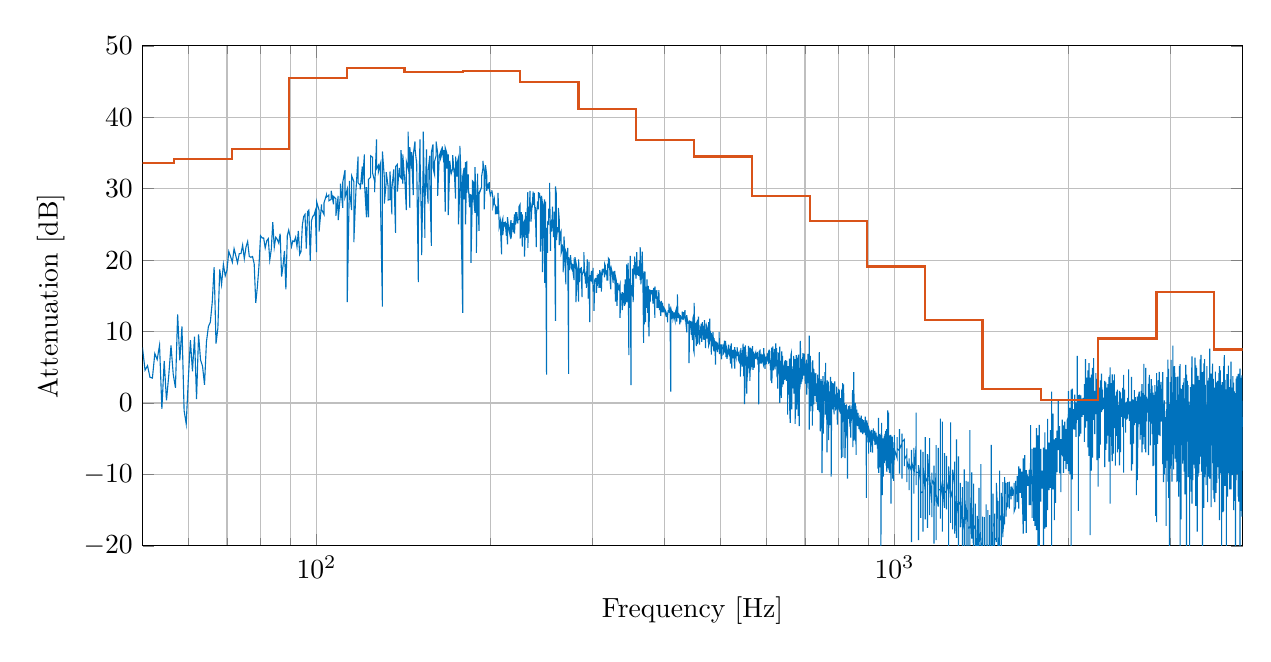
\begin{tikzpicture}

\begin{axis}[%
width=5.5in,
height=2.5in,
at={(1.011in,0.642in)},
scale only axis,
unbounded coords=jump,
xmode=log,
xmin=50,
xmax=4e+03,
xminorticks=true,
xlabel={Frequency [Hz]},
xmajorgrids,
xminorgrids,
ymin=-20,
ymax=50,
ylabel={Attenuation [dB]},
ymajorgrids,
axis background/.style={fill=white},
title style={font=\bfseries},
legend style={at={(0.03,0.03)},anchor=south west,legend cell align=left,align=left,draw=white!15!black}
]

\addplot [color=mycolor1,solid,forget plot]
  table[row sep=crcr]{%
0	4.25\\
0.5	0.299\\
1	-0.129\\
1.5	-0.698\\
2	-5.55\\
2.5	-2.38\\
3	5.66\\
3.5	9.04\\
4	2.93\\
4.5	1.46\\
5	-0.368\\
5.5	-7.72\\
6	4.23\\
6.5	-0.568\\
7	-2.5\\
7.5	0.628\\
8	1.71\\
8.5	3.48\\
9	-2.31\\
9.5	1.19\\
10	0.619\\
10.5	1.34\\
11	0.0477\\
11.5	-3.6\\
12	2.1\\
12.5	3.56\\
13	-1.5\\
13.5	1.18\\
14	-0.846\\
14.5	0.81\\
15	3.43\\
15.5	-1.56\\
16	2.25\\
16.5	0.483\\
17	-0.528\\
17.5	-0.793\\
18	11.8\\
18.5	4.83\\
19	8.21\\
19.5	10.3\\
20	3.69\\
20.5	1.78\\
21	-0.0409\\
21.5	9.31\\
22	3.52\\
22.5	5.81\\
23	2.74\\
23.5	5.05\\
24	10.3\\
24.5	8.06\\
25	4.91\\
25.5	1.45\\
26	13\\
26.5	4.22\\
27	5.55\\
27.5	-3.34\\
28	9.36\\
28.5	9.05\\
29	8.89\\
29.5	7.44\\
30	0.271\\
30.5	7.43\\
31	13\\
31.5	14.2\\
32	15.3\\
32.5	12\\
33	14.4\\
33.5	9.54\\
34	8.3\\
34.5	2.7\\
35	8.17\\
35.5	7.62\\
36	10.4\\
36.5	8.87\\
37	-1.52\\
37.5	6.8\\
38	3.46\\
38.5	3.63\\
39	5.7\\
39.5	3.4\\
40	-0.995\\
40.5	4.47\\
41	8.92\\
41.5	10.3\\
42	14.8\\
42.5	-0.628\\
43	-10.4\\
43.5	3.69\\
44	0.807\\
44.5	5.37\\
45	4.45\\
45.5	-6.89\\
46	3.74\\
46.5	8.2\\
47	-8.8\\
47.5	-1.76\\
48	-0.381\\
48.5	0.505\\
49	9.4\\
49.5	7.36\\
50	7.64\\
50.5	4.59\\
51	5.21\\
51.5	3.59\\
52	3.48\\
52.5	6.91\\
53	6.08\\
53.5	8.07\\
54	-0.821\\
54.5	5.87\\
55	0.358\\
55.5	3.82\\
56	8.06\\
56.5	4.02\\
57	2.13\\
57.5	12.4\\
58	5.96\\
58.5	10.7\\
59	-1.06\\
59.5	-2.94\\
60	3.29\\
60.5	8.8\\
61	4.42\\
61.5	9.27\\
62	0.531\\
62.5	9.58\\
63	6\\
63.5	5.15\\
64	2.54\\
64.5	8.56\\
65	10.7\\
65.5	11.3\\
66	14.1\\
66.5	19\\
67	8.3\\
67.5	10.5\\
68	18.7\\
68.5	16.6\\
69	19.4\\
69.5	17.8\\
70	18.6\\
70.5	21.2\\
71	20.5\\
71.5	19.7\\
72	21.6\\
72.5	20.6\\
73	19.6\\
73.5	20.9\\
74	20.9\\
74.5	22.1\\
75	20.2\\
75.5	21.8\\
76	22.6\\
76.5	20.5\\
77	20.4\\
77.5	20.5\\
78	19.5\\
78.5	14\\
79	16.2\\
79.5	19.1\\
80	23.4\\
80.5	23.1\\
81	23.1\\
81.5	21.7\\
82	22.7\\
82.5	23\\
83	20\\
83.5	21.5\\
84	25.3\\
84.5	21.8\\
85	23.2\\
85.5	22.9\\
86	22.4\\
86.5	23.7\\
87	17.7\\
87.5	19.2\\
88	21.3\\
88.5	15.9\\
89	23.4\\
89.5	24.2\\
90	23.3\\
90.5	21.9\\
91	22.7\\
91.5	22.6\\
92	23.2\\
92.5	21.9\\
93	24.1\\
93.5	20.8\\
94	21.2\\
94.5	24.9\\
95	26.1\\
95.5	26.4\\
96	21.6\\
96.5	26.8\\
97	27\\
97.5	19.9\\
98	25.5\\
98.5	26.1\\
99	26.3\\
99.5	26.9\\
100	21.1\\
100	28.2\\
101	27\\
101	24\\
102	27.8\\
102	27.1\\
103	26.4\\
103	28\\
104	29.1\\
104	28.8\\
105	29.1\\
105	28.3\\
106	28.5\\
106	29.7\\
107	27.8\\
107	28.9\\
108	28.6\\
108	26.2\\
109	29\\
109	25.6\\
110	29.2\\
110	30.7\\
111	27.3\\
111	30.9\\
112	32.6\\
112	28.8\\
113	29.9\\
113	14.1\\
114	31.1\\
114	29.9\\
115	27\\
115	31.8\\
116	31\\
116	22.5\\
117	29.9\\
117	29.8\\
118	34.5\\
118	30.8\\
119	30.5\\
119	29.9\\
120	33.1\\
120	30.6\\
121	34.8\\
121	30.9\\
122	26\\
122	30.2\\
123	26\\
123	31.3\\
124	31.6\\
124	34.6\\
125	34.4\\
125	32.2\\
126	31.1\\
126	29.5\\
127	36.9\\
127	32.8\\
128	33.3\\
128	32.4\\
129	33.5\\
129	28.5\\
130	13.5\\
130	35.2\\
131	31.6\\
131	27.9\\
132	31\\
132	32.3\\
133	30.3\\
133	28.4\\
134	28.5\\
134	32.4\\
135	26.4\\
135	30\\
136	32.7\\
136	32.5\\
137	23.8\\
137	33.1\\
138	33.4\\
138	29.6\\
139	32.9\\
139	31.9\\
140	31.5\\
140	35.4\\
141	30.7\\
141	34.8\\
142	31.2\\
142	32\\
143	27\\
143	33.8\\
144	32.8\\
144	38\\
145	27.3\\
145	35.8\\
146	32.8\\
146	35.1\\
147	29.1\\
147	34.7\\
148	36.6\\
148	35.7\\
149	33.5\\
149	34\\
150	16.9\\
150	25.7\\
151	36.9\\
151	34.7\\
152	23.5\\
152	20.7\\
153	34.5\\
153	38\\
154	23.1\\
154	27.8\\
155	35.5\\
155	31\\
156	27.9\\
156	32.6\\
157	34.6\\
157	31.4\\
158	22\\
158	35.1\\
159	36.2\\
159	32.9\\
160	32\\
160	33.8\\
161	34.6\\
161	36.6\\
162	35\\
162	29\\
163	34.3\\
163	34.6\\
164	35.2\\
164	34.3\\
165	35\\
165	35.9\\
166	33.7\\
166	35.4\\
167	26.8\\
167	35.7\\
168	35\\
168	32.8\\
169	34.8\\
169	26.3\\
170	33.5\\
170	33.9\\
171	32.1\\
171	32.1\\
172	32.8\\
172	34.7\\
173	32.2\\
173	32.9\\
174	28.6\\
174	34.5\\
175	31.7\\
175	33.5\\
176	34.3\\
176	25\\
177	30.3\\
177	36\\
178	30.6\\
178	24.4\\
179	12.6\\
179	31.7\\
180	32.9\\
180	28.5\\
181	33.7\\
181	25\\
182	33.9\\
182	29.4\\
183	32\\
183	30.7\\
184	27.4\\
184	29.2\\
185	29.1\\
185	19.6\\
186	28.9\\
186	31.1\\
187	30.9\\
187	28.7\\
188	26.6\\
188	33\\
189	27.1\\
189	21\\
190	32.1\\
190	30.7\\
191	24.1\\
191	29.4\\
192	29.8\\
192	29.7\\
193	30.2\\
193	31.7\\
194	32.8\\
194	33.9\\
195	32.4\\
195	27.1\\
196	32.5\\
196	33.3\\
197	31.9\\
197	29.7\\
198	30.7\\
198	30\\
199	30.9\\
199	30\\
200	28.9\\
200	29.4\\
201	29.5\\
201	29.8\\
202	28.6\\
202	27.6\\
203	28.4\\
203	27.9\\
204	27.6\\
204	26.4\\
205	27.5\\
205	26.5\\
206	26.5\\
206	29.4\\
207	25.2\\
207	24.7\\
208	25.5\\
208	24.8\\
209	20.8\\
209	25.2\\
210	25.8\\
210	23.5\\
211	25.3\\
211	25\\
212	24.7\\
212	25.4\\
213	23.4\\
213	25.2\\
214	22.2\\
214	26\\
215	24.2\\
215	24.4\\
216	23.6\\
216	24.5\\
217	25.6\\
217	23\\
218	24.6\\
218	25.1\\
219	25.1\\
219	23.9\\
220	26.4\\
220	23.7\\
221	26.7\\
221	25\\
222	25.9\\
222	26.7\\
223	25.1\\
223	25.6\\
224	25.7\\
224	27.5\\
225	27.8\\
225	23\\
226	24.7\\
226	26.7\\
227	21.9\\
227	26.4\\
228	23.2\\
228	25.1\\
229	25.5\\
229	20.5\\
230	26.7\\
230	25.9\\
231	23.1\\
231	24.7\\
232	29.5\\
232	21.7\\
233	27.5\\
233	23.7\\
234	29.7\\
234	28.5\\
235	26.5\\
235	25.4\\
236	28\\
236	27.3\\
237	29.6\\
237	27.7\\
238	29\\
238	29.4\\
239	25.7\\
239	27.4\\
240	21.8\\
240	26.5\\
241	27.6\\
241	28.2\\
242	27.1\\
242	29.5\\
243	28.7\\
243	29.4\\
244	28.2\\
244	21.2\\
245	25\\
245	29\\
246	27.9\\
246	18.3\\
247	25.5\\
247	27.1\\
248	28.5\\
248	16.8\\
249	28.2\\
249	27.7\\
250	3.96\\
250	24.5\\
251	21\\
251	25.3\\
252	25.1\\
252	27.2\\
253	25.9\\
253	30.8\\
254	21.3\\
254	25.1\\
255	25.5\\
255	24\\
256	27\\
256	27.5\\
257	23.2\\
257	23.6\\
258	26.1\\
258	26.8\\
259	11.5\\
259	30.3\\
260	29.2\\
260	22.8\\
261	24.3\\
261	24.6\\
262	23.9\\
262	27.3\\
263	25.6\\
263	22.1\\
264	23.4\\
264	23.8\\
265	24.1\\
265	21\\
266	21.5\\
266	22.2\\
267	21.3\\
267	18.3\\
268	20.5\\
268	23.3\\
269	20.2\\
269	20.2\\
270	16.6\\
270	21.2\\
271	20.8\\
271	21\\
272	19.3\\
272	21.7\\
273	4.06\\
273	20.4\\
274	19.3\\
274	18.6\\
275	20.6\\
275	20.7\\
276	19.3\\
276	18.9\\
277	18.6\\
277	19.4\\
278	19.3\\
278	18.1\\
279	17.2\\
279	19.7\\
280	19.2\\
280	20.4\\
281	19.4\\
281	14.1\\
282	16.9\\
282	19.1\\
283	18.5\\
283	18.5\\
284	14.2\\
284	20.1\\
285	16.9\\
285	18.8\\
286	18.2\\
286	18.8\\
287	18.9\\
287	18.6\\
288	14.8\\
288	17.9\\
289	18.3\\
289	18.2\\
290	18.3\\
290	21.1\\
291	17.8\\
291	18.3\\
292	16.9\\
292	16.7\\
293	18.4\\
293	16.1\\
294	20.1\\
294	17\\
295	16.8\\
295	14.6\\
296	18.3\\
296	19.8\\
297	11.3\\
297	17.9\\
298	17.1\\
298	17.3\\
299	18.5\\
299	17\\
300	17.7\\
300	16.7\\
301	18.9\\
301	15.6\\
302	16.5\\
302	12.9\\
303	17.4\\
303	17.1\\
304	17.4\\
304	17.5\\
305	16.8\\
305	15.4\\
306	17.9\\
306	16.4\\
307	17.8\\
307	18\\
308	17.9\\
308	16.1\\
309	18.6\\
309	17.5\\
310	17.9\\
310	16.1\\
311	17.8\\
311	15.6\\
312	18.7\\
312	17.9\\
313	18.8\\
313	18.6\\
314	18.4\\
314	18.8\\
315	17.6\\
315	19.5\\
316	19.2\\
316	19\\
317	17.9\\
317	18.6\\
318	17.7\\
318	17.2\\
319	17.2\\
319	19.5\\
320	18.9\\
320	20.2\\
321	20\\
321	20.2\\
322	17.7\\
322	17\\
323	15.9\\
323	18.7\\
324	18.3\\
324	18.6\\
325	18.1\\
325	17.8\\
326	16.8\\
326	18.4\\
327	17.2\\
327	17.4\\
328	17.2\\
328	18.5\\
329	14.2\\
329	17.7\\
330	17.2\\
330	16.7\\
331	16.6\\
331	13.6\\
332	16.7\\
332	16.8\\
333	16.2\\
333	16\\
334	15.8\\
334	16.2\\
335	16.6\\
335	11.9\\
336	15\\
336	15.1\\
337	14.7\\
337	14.8\\
338	15.5\\
338	13\\
339	14.8\\
339	15.4\\
340	14.1\\
340	14.3\\
341	13.6\\
341	16.6\\
342	13.8\\
342	17.3\\
343	15\\
343	16.8\\
344	14.1\\
344	19.4\\
345	14.2\\
345	17.2\\
346	14\\
346	19.6\\
347	6.69\\
347	17.4\\
348	13.3\\
348	16.1\\
349	14.1\\
349	20.6\\
350	2.51\\
350	14.8\\
351	16.5\\
351	15.4\\
352	15.1\\
352	18.8\\
353	17.9\\
353	14.1\\
354	19.3\\
354	18.4\\
355	18.2\\
355	20.5\\
356	19\\
356	19.1\\
357	17.4\\
357	19.5\\
358	19.8\\
358	21.1\\
359	17.9\\
359	18.6\\
360	18.4\\
360	19.1\\
361	17.8\\
361	19\\
362	17.9\\
362	20\\
363	17.2\\
363	21.8\\
364	18.9\\
364	16.6\\
365	17.9\\
365	18.3\\
366	17.4\\
366	21.2\\
367	16.7\\
367	17\\
368	8.41\\
368	17.7\\
369	18.4\\
369	11\\
370	18.4\\
370	18.3\\
371	11.3\\
371	16.3\\
372	13.3\\
372	15.4\\
373	13.7\\
373	17.3\\
374	14.2\\
374	12.6\\
375	16.4\\
375	10.6\\
376	12.2\\
376	9.33\\
377	15.9\\
377	14.8\\
378	14.2\\
378	15.3\\
379	15.8\\
379	15.5\\
380	15.4\\
380	15.2\\
381	15.8\\
381	15.5\\
382	13.9\\
382	14\\
383	16.1\\
383	15.1\\
384	14.6\\
384	14.6\\
385	11.9\\
385	16.3\\
386	15\\
386	14.6\\
387	15.1\\
387	14.8\\
388	15.8\\
388	13.3\\
389	13.9\\
389	14.9\\
390	13.3\\
390	13.3\\
391	15.6\\
391	15.8\\
392	13.4\\
392	13\\
393	14.2\\
393	13.5\\
394	12.2\\
394	13.6\\
395	13.5\\
395	14.3\\
396	13.1\\
396	12.7\\
397	14\\
397	13.6\\
398	13.5\\
398	12.7\\
399	13.3\\
399	13.3\\
400	13.2\\
400	12.9\\
401	12.6\\
401	13\\
402	12.8\\
402	12.8\\
403	12.5\\
403	12.2\\
404	12.3\\
404	12.6\\
405	11.3\\
405	12.3\\
406	13\\
406	12.9\\
407	12.8\\
407	13.9\\
408	12.7\\
408	12.9\\
409	12.7\\
409	11.3\\
410	1.58\\
410	12.8\\
411	12.4\\
411	12.9\\
412	12.5\\
412	11.8\\
413	12.9\\
413	12.6\\
414	12.5\\
414	11.9\\
415	12.3\\
415	12.6\\
416	12.6\\
416	12\\
417	11.6\\
417	12.5\\
418	12.7\\
418	12.8\\
419	13.1\\
419	12.6\\
420	11.4\\
420	12.7\\
421	12.1\\
421	15.2\\
422	11.9\\
422	11.9\\
423	12.5\\
423	12.6\\
424	12\\
424	12.4\\
425	11.4\\
425	11\\
426	12.3\\
426	12.3\\
427	11.3\\
427	12\\
428	12\\
428	11.9\\
429	11.8\\
429	12.8\\
430	11.7\\
430	11.9\\
431	11.8\\
431	12.7\\
432	12.1\\
432	12.5\\
433	11.9\\
433	12.5\\
434	13\\
434	11.8\\
435	11.4\\
435	12.1\\
436	10.7\\
436	11.3\\
437	9.87\\
437	12.3\\
438	11.5\\
438	11.8\\
439	11.1\\
439	11.5\\
440	11.1\\
440	11.3\\
441	11.2\\
441	5.56\\
442	11.3\\
442	11.4\\
443	11.3\\
443	10.5\\
444	10.9\\
444	11.5\\
445	10.2\\
445	9.52\\
446	11.4\\
446	10.3\\
447	8.81\\
447	10.7\\
448	9.75\\
448	11.9\\
449	12.2\\
449	7.44\\
450	7.08\\
450	14\\
451	10.6\\
451	9.9\\
452	11.2\\
452	9.88\\
453	9.27\\
453	10\\
454	7.96\\
454	11.1\\
455	11.3\\
455	9.67\\
456	8.22\\
456	11.6\\
457	10.5\\
457	10\\
458	12.1\\
458	10.6\\
459	8.34\\
459	10.2\\
460	8.16\\
460	10\\
461	9.06\\
461	10.5\\
462	10.3\\
462	10.4\\
463	9.03\\
463	11.1\\
464	8.56\\
464	9.7\\
465	10\\
465	11.3\\
466	9.48\\
466	10.5\\
467	10.5\\
467	8.88\\
468	9.53\\
468	10.8\\
469	8.83\\
469	11.6\\
470	9.11\\
470	11.1\\
471	7.66\\
471	10.1\\
472	10.2\\
472	9.79\\
473	9.01\\
473	10.7\\
474	10.4\\
474	9.38\\
475	9.26\\
475	10.2\\
476	8.47\\
476	10.3\\
477	11.3\\
477	8.08\\
478	8.32\\
478	9.56\\
479	11.8\\
479	9.39\\
480	8.73\\
480	10.1\\
481	8.63\\
481	9.82\\
482	6.76\\
482	9.81\\
483	8.21\\
483	8.9\\
484	9.03\\
484	8.15\\
485	7.98\\
485	9.94\\
486	8.64\\
486	7.73\\
487	7.24\\
487	9.06\\
488	8.54\\
488	8.11\\
489	8.66\\
489	8.69\\
490	5.38\\
490	7.08\\
491	7.5\\
491	8.43\\
492	7.9\\
492	8.59\\
493	8.03\\
493	7.81\\
494	8.43\\
494	7.11\\
495	8.15\\
495	7.94\\
496	8.02\\
496	7.94\\
497	7.69\\
497	9.95\\
498	6.82\\
498	7.39\\
499	7.85\\
499	8.23\\
500	7.41\\
500	6.98\\
501	8.12\\
501	7\\
502	6.12\\
502	7.69\\
503	8.21\\
503	7.94\\
504	7.55\\
504	7.74\\
505	7.71\\
505	6.83\\
506	6.92\\
506	7.81\\
507	7.57\\
507	7.73\\
508	8.34\\
508	8.73\\
509	7.9\\
509	7.36\\
510	7.1\\
510	8.67\\
511	7.67\\
511	6.43\\
512	7.08\\
512	7.68\\
513	6.16\\
513	7.41\\
514	7.1\\
514	6.41\\
515	7.07\\
515	6.82\\
516	7.28\\
516	8.15\\
517	6.91\\
517	7.13\\
518	6.83\\
518	7.56\\
519	6.96\\
519	7.6\\
520	5.52\\
520	7.41\\
521	7.13\\
521	7.79\\
522	8.34\\
522	6.14\\
523	4.82\\
523	6.68\\
524	7.44\\
524	6.33\\
525	6.75\\
525	7.2\\
526	6.23\\
526	7.12\\
527	7.46\\
527	7.23\\
528	6.23\\
528	5.87\\
529	4.82\\
529	7.82\\
530	6.54\\
530	7.29\\
531	6.96\\
531	6.71\\
532	6.4\\
532	6.91\\
533	6.68\\
533	6.62\\
534	6.63\\
534	7.81\\
535	7.15\\
535	6.89\\
536	6.84\\
536	6.89\\
537	6.97\\
537	6.04\\
538	5.88\\
538	5.9\\
539	6.18\\
539	6.08\\
540	6.76\\
540	6.16\\
541	7.44\\
541	3.69\\
542	7.16\\
542	7.69\\
543	6.58\\
543	5.98\\
544	6.65\\
544	5.36\\
545	6.97\\
545	5.09\\
546	6.2\\
546	6.95\\
547	8.31\\
547	6.36\\
548	7.81\\
548	3.79\\
549	7.11\\
549	7.86\\
550	0.724\\
550	-0.173\\
551	2.29\\
551	1.99\\
552	8.06\\
552	7.66\\
553	6.56\\
553	7.1\\
554	5.22\\
554	6.46\\
555	4.53\\
555	1.29\\
556	5.32\\
556	3.61\\
557	6.46\\
557	4.05\\
558	6.93\\
558	6.55\\
559	7.98\\
559	6.35\\
560	5.66\\
560	4.85\\
561	6.74\\
561	7.76\\
562	3.08\\
562	3.53\\
563	5.12\\
563	7.74\\
564	6.78\\
564	4.7\\
565	7.6\\
565	6.52\\
566	5.03\\
566	6.3\\
567	5.87\\
567	6.43\\
568	7.97\\
568	6.34\\
569	4.83\\
569	4.64\\
570	7.19\\
570	6\\
571	6.58\\
571	6.57\\
572	4.93\\
572	6.91\\
573	6.16\\
573	6.75\\
574	6.24\\
574	6.78\\
575	7\\
575	6.5\\
576	6.62\\
576	6.12\\
577	6.71\\
577	7\\
578	6.69\\
578	6.77\\
579	6.26\\
579	7.16\\
580	5.95\\
580	5.36\\
581	6.33\\
581	6.28\\
582	6.36\\
582	-0.202\\
583	7.28\\
583	5.45\\
584	5.85\\
584	6.28\\
585	6.06\\
585	7.48\\
586	6.28\\
586	6.25\\
587	6.61\\
587	5.89\\
588	6.81\\
588	5.5\\
589	5.88\\
589	6.29\\
590	5.72\\
590	6.31\\
591	6.02\\
591	6.79\\
592	6.39\\
592	6.2\\
593	6.11\\
593	6.13\\
594	7.68\\
594	5.46\\
595	5.66\\
595	5.77\\
596	6.22\\
596	6.29\\
597	4.76\\
597	6.35\\
598	6.13\\
598	6.35\\
599	6.05\\
599	5.36\\
600	6.47\\
600	5.47\\
601	6.53\\
601	5.81\\
602	6.3\\
602	6.93\\
603	6.09\\
603	6.54\\
604	6.78\\
604	5.94\\
605	6.57\\
605	5.57\\
606	5.63\\
606	5.68\\
607	7.47\\
607	6.29\\
608	6.16\\
608	5.85\\
609	5.95\\
609	6\\
610	4.61\\
610	4.98\\
611	4.65\\
611	3.13\\
612	7.25\\
612	5.54\\
613	7.75\\
613	2.77\\
614	3.89\\
614	6.15\\
615	6.7\\
615	5.38\\
616	7.93\\
616	6.69\\
617	4.56\\
617	7.08\\
618	4.99\\
618	7\\
619	5.13\\
619	5.3\\
620	5.49\\
620	7.57\\
621	5.8\\
621	4.69\\
622	6.56\\
622	5.87\\
623	8.33\\
623	7.37\\
624	5.81\\
624	5.12\\
625	6.76\\
625	7.66\\
626	3.67\\
626	7.13\\
627	4.07\\
627	4.76\\
628	2.01\\
628	4.7\\
629	5.57\\
629	6.03\\
630	4.69\\
630	7.06\\
631	5.74\\
631	5.17\\
632	3.87\\
632	4.76\\
633	7.89\\
633	0.026\\
634	5.82\\
634	5.97\\
635	4.13\\
635	3.86\\
636	5.87\\
636	3.91\\
637	0.719\\
637	4.04\\
638	7.23\\
638	6.19\\
639	5.29\\
639	2.21\\
640	6.6\\
640	3.87\\
641	5.51\\
641	5.35\\
642	4.91\\
642	2.6\\
643	3.32\\
643	4.47\\
644	5.12\\
644	4.97\\
645	3.22\\
645	5.03\\
646	5.91\\
646	5.69\\
647	5.67\\
647	3.29\\
648	4.85\\
648	5.99\\
649	5.33\\
649	5.68\\
650	5.21\\
650	3.1\\
651	5.9\\
651	4.97\\
652	3.63\\
652	3.99\\
653	5.03\\
653	-1.64\\
654	5.15\\
654	3.68\\
655	3.16\\
655	3.69\\
656	4.59\\
656	1.15\\
657	4.86\\
657	3.73\\
658	6.22\\
658	5\\
659	-2.2\\
659	4.23\\
660	-2.79\\
660	1.74\\
661	2.81\\
661	1.38\\
662	5.31\\
662	6.77\\
663	7\\
663	3.77\\
664	-0.887\\
664	0.928\\
665	5.12\\
665	4.47\\
666	2.9\\
666	2.03\\
667	4.36\\
667	2.35\\
668	2.96\\
668	4.75\\
669	3.74\\
669	6.58\\
670	4.65\\
670	1.32\\
671	4.97\\
671	5.67\\
672	3.25\\
672	3.49\\
673	6.15\\
673	-2.92\\
674	2.76\\
674	-0.96\\
675	3.44\\
675	4.31\\
676	3.9\\
676	6.71\\
677	-0.15\\
677	-0.892\\
678	3.29\\
678	5.92\\
679	6.08\\
679	4.34\\
680	2.76\\
680	4.96\\
681	4.12\\
681	-1.82\\
682	2.17\\
682	6.76\\
683	1.63\\
683	3.21\\
684	-3.26\\
684	3.65\\
685	1.89\\
685	4.92\\
686	3.84\\
686	1.9\\
687	8.68\\
687	4.57\\
688	7.67\\
688	5.34\\
689	2.65\\
689	4.3\\
690	3.82\\
690	6.16\\
691	2.99\\
691	4.82\\
692	5.47\\
692	4.17\\
693	4.8\\
693	3.34\\
694	6.98\\
694	4.47\\
695	5.56\\
695	4.13\\
696	4.63\\
696	5.5\\
697	3.84\\
697	5.02\\
698	4.55\\
698	6.92\\
699	4.46\\
699	5.55\\
700	4.8\\
700	4.91\\
701	2.71\\
701	4.42\\
702	4.2\\
702	3.32\\
703	3.54\\
703	4.91\\
704	6.05\\
704	3.59\\
705	5.54\\
705	1.16\\
706	3.55\\
706	3.86\\
707	3.4\\
707	3.52\\
708	2.78\\
708	6.86\\
709	4.73\\
709	6.7\\
710	3.04\\
710	5.04\\
711	3.75\\
711	1.98\\
712	9.43\\
712	-3.73\\
713	3.83\\
713	0.858\\
714	3.23\\
714	-1.17\\
715	6.59\\
715	2\\
716	3.82\\
716	5.74\\
717	-0.444\\
717	2.15\\
718	2.06\\
718	3.01\\
719	0.00692\\
719	4.29\\
720	2.89\\
720	2.67\\
721	-3.16\\
721	0.448\\
722	-1.17\\
722	5.96\\
723	3.73\\
723	1.73\\
724	2.9\\
724	3.68\\
725	-0.192\\
725	4.75\\
726	1.5\\
726	4.3\\
727	2.44\\
727	3.13\\
728	0.975\\
728	3.33\\
729	3.69\\
729	3.65\\
730	3.3\\
730	3.88\\
731	4.18\\
731	1\\
732	2.2\\
732	0.315\\
733	2.39\\
733	0.15\\
734	2.12\\
734	2.65\\
735	2.67\\
735	2.22\\
736	-0.985\\
736	3.95\\
737	-0.2\\
737	1.59\\
738	2.46\\
738	-0.833\\
739	3.04\\
739	-0.481\\
740	-1.06\\
740	2.24\\
741	7.11\\
741	-1.27\\
742	-0.0282\\
742	2\\
743	0.982\\
743	1.17\\
744	-3.97\\
744	-3.85\\
745	3.1\\
745	2.53\\
746	3.35\\
746	3.25\\
747	-3.55\\
747	-2.88\\
748	-0.921\\
748	-1.16\\
749	-5.44\\
749	-9.84\\
750	-5.05\\
750	3.04\\
751	0.29\\
751	1.6\\
752	3.75\\
752	1.82\\
753	-4.31\\
753	-1.78\\
754	2.38\\
754	-2.89\\
755	2.1\\
755	2.5\\
756	1.11\\
756	1.77\\
757	2.97\\
757	1.01\\
758	1.02\\
758	4.33\\
759	0.148\\
759	-1.64\\
760	5.6\\
760	1.33\\
761	1.43\\
761	2.71\\
762	1.25\\
762	-0.733\\
763	-0.0766\\
763	2.74\\
764	-6.91\\
764	-4.81\\
765	3.17\\
765	-1.88\\
766	-3.03\\
766	1.79\\
767	1.69\\
767	2.81\\
768	-0.229\\
768	2.98\\
769	-2.77\\
769	-5.22\\
770	0.237\\
770	1.61\\
771	-2.38\\
771	-1.98\\
772	-1.25\\
772	0.43\\
773	-3.12\\
773	-0.956\\
774	2.43\\
774	0.307\\
775	0.173\\
775	3.64\\
776	-0.384\\
776	0.994\\
777	0.795\\
777	-10.3\\
778	-2.7\\
778	3.03\\
779	1.66\\
779	0.316\\
780	1.92\\
780	1.85\\
781	-0.357\\
781	-0.891\\
782	2.77\\
782	-0.385\\
783	1.7\\
783	2.62\\
784	0.876\\
784	1.69\\
785	1.56\\
785	1.03\\
786	-1.61\\
786	2.72\\
787	-0.123\\
787	0.842\\
788	3.03\\
788	0.531\\
789	1.02\\
789	-0.204\\
790	-0.544\\
790	0.0196\\
791	0.986\\
791	-0.873\\
792	-0.804\\
792	1.02\\
793	1.15\\
793	1.15\\
794	0.0337\\
794	2.28\\
795	1.7\\
795	0.233\\
796	0.85\\
796	-2.14\\
797	-3.03\\
797	-2.67\\
798	1.29\\
798	-0.466\\
799	1.4\\
799	0.079\\
800	-0.348\\
800	1.97\\
801	0.444\\
801	1.16\\
802	-0.995\\
802	1.86\\
803	0.252\\
803	-0.923\\
804	-0.179\\
804	-1.22\\
805	0.298\\
805	-1.37\\
806	0.682\\
806	-1.48\\
807	0.642\\
807	0.596\\
808	0.166\\
808	-0.621\\
809	-7.73\\
809	-0.459\\
810	-2.71\\
810	1.86\\
811	0.136\\
811	0.4\\
812	0.625\\
812	-2.29\\
813	2.78\\
813	2.01\\
814	-2.87\\
814	-7.58\\
815	1.61\\
815	-1.56\\
816	-0.754\\
816	2.59\\
817	0.52\\
817	-2.62\\
818	-0.339\\
818	-1.41\\
819	-2.23\\
819	-0.0333\\
820	-1.91\\
820	-4.04\\
821	-0.72\\
821	-7.71\\
822	-4.69\\
822	-1.55\\
823	-0.32\\
823	-4.95\\
824	-1.28\\
824	-1.13\\
825	-0.763\\
825	-1.53\\
826	-1.51\\
826	-0.204\\
827	-1.56\\
827	-1.5\\
828	-0.856\\
828	-1.06\\
829	-10.6\\
829	-1.15\\
830	-1.91\\
830	-2.23\\
831	-0.975\\
831	-1.47\\
832	-1.58\\
832	-2.21\\
833	-1.71\\
833	-0.431\\
834	-1.33\\
834	-1.18\\
835	-2.05\\
835	-1.77\\
836	-1.64\\
836	-1.82\\
837	-3.31\\
837	-0.271\\
838	-1.98\\
838	-2.24\\
839	-3.63\\
839	-1.84\\
840	-2.36\\
840	-4.86\\
841	-0.878\\
841	-2.07\\
842	-1.97\\
842	-2.51\\
843	-1.42\\
843	-2.02\\
844	-1.58\\
844	-0.365\\
845	-1.06\\
845	-1.98\\
846	1.81\\
846	-2.22\\
847	-1.97\\
847	-6.19\\
848	-0.586\\
848	-3.23\\
849	-5.26\\
849	-2.06\\
850	-0.0224\\
850	4.3\\
851	-0.577\\
851	-3.19\\
852	-5.04\\
852	-1.22\\
853	-5.14\\
853	-4.39\\
854	-1.48\\
854	-4.06\\
855	-2.83\\
855	0.0103\\
856	-5.22\\
856	-5.33\\
857	-1.18\\
857	-0.401\\
858	-7.28\\
858	-2.37\\
859	-2.84\\
859	-1.86\\
860	-3.19\\
860	-0.92\\
861	-2.86\\
861	-1.91\\
862	-2.06\\
862	-2.06\\
863	-3.23\\
863	-2.29\\
864	-2.26\\
864	-1.92\\
865	-1.38\\
865	-2.12\\
866	-2.75\\
866	-2.62\\
867	-2.43\\
867	-2.49\\
868	-2.4\\
868	-3.68\\
869	-2.74\\
869	-2.65\\
870	-2.82\\
870	-2.61\\
871	-2.09\\
871	-2.37\\
872	-3.92\\
872	-2.73\\
873	-4.12\\
873	-3.23\\
874	-2.91\\
874	-2.12\\
875	-3.61\\
875	-2.07\\
876	-1.77\\
876	-3.12\\
877	-2.74\\
877	-2.41\\
878	-3.16\\
878	-4.16\\
879	-3.29\\
879	-2.26\\
880	-3.69\\
880	-3.4\\
881	-3.22\\
881	-4.35\\
882	-3.89\\
882	-3.08\\
883	-3.65\\
883	-3.69\\
884	-2.42\\
884	-2.78\\
885	-3.22\\
885	-3.29\\
886	-2.74\\
886	-4.16\\
887	-2.72\\
887	-3.53\\
888	-3.11\\
888	-3.39\\
889	-3.22\\
889	-4.05\\
890	-1.9\\
890	-4.51\\
891	-3.01\\
891	-2.87\\
892	-3.29\\
892	-4.08\\
893	-4.06\\
893	-3.63\\
894	-13.3\\
894	-4.81\\
895	-4.72\\
895	-2.44\\
896	-4.32\\
896	-3.7\\
897	-3.51\\
897	-4.82\\
898	-4.07\\
898	-3.82\\
899	-3.26\\
899	-5.51\\
900	-4.35\\
900	-4.22\\
901	-4.04\\
901	-3.16\\
902	-7.09\\
902	-4.87\\
903	-4.65\\
903	-3.71\\
904	-4.25\\
904	-3.86\\
905	-4.02\\
905	-5.51\\
906	-4.19\\
906	-4.13\\
907	-4.17\\
907	-4.87\\
908	-4.81\\
908	-4.37\\
909	-4.22\\
909	-6.89\\
910	-4.42\\
910	-4.71\\
911	-4.69\\
911	-4.21\\
912	-4.42\\
912	-4.03\\
913	-3.81\\
913	-4.78\\
914	-5\\
914	-5.17\\
915	-4.98\\
915	-4.98\\
916	-6.95\\
916	-4.37\\
917	-4.59\\
917	-4.66\\
918	-4.63\\
918	-5.3\\
919	-4.26\\
919	-3.57\\
920	-4.53\\
920	-4.31\\
921	-4.35\\
921	-4.82\\
922	-4.83\\
922	-4.2\\
923	-4.97\\
923	-5.1\\
924	-3.9\\
924	-5.43\\
925	-4.25\\
925	-5.88\\
926	-4.75\\
926	-4.94\\
927	-5.81\\
927	-4.83\\
928	-5.79\\
928	-5.31\\
929	-4.16\\
929	-5.21\\
930	-5.13\\
930	-4.95\\
931	-4.66\\
931	-5.65\\
932	-4.59\\
932	-4.74\\
933	-5.43\\
933	-5.42\\
934	-6.4\\
934	-5.42\\
935	-4.99\\
935	-6.07\\
936	-5.05\\
936	-9.19\\
937	-4.77\\
937	-5.21\\
938	-4.76\\
938	-2.08\\
939	-5.14\\
939	-9.79\\
940	-6.34\\
940	-6.14\\
941	-5.5\\
941	-5.49\\
942	-4.37\\
942	-9.03\\
943	-6.77\\
943	-5.03\\
944	-4.68\\
944	-5.62\\
945	-4.51\\
945	-7.52\\
946	-6.38\\
946	-4.77\\
947	-4.9\\
947	-20.3\\
948	-10.4\\
948	-4.66\\
949	-9.74\\
949	-8.22\\
950	-2.79\\
950	-4.46\\
951	-5.15\\
951	-7.09\\
952	-8.16\\
952	-12.9\\
953	-5.18\\
953	-6.79\\
954	-5.05\\
954	-7.61\\
955	-5.26\\
955	-4.97\\
956	-10.3\\
956	-6.64\\
957	-7.67\\
957	-7.12\\
958	-6.6\\
958	-7.72\\
959	-5.89\\
959	-4.86\\
960	-4.89\\
960	-8.43\\
961	-7.58\\
961	-6.42\\
962	-4.32\\
962	-6.38\\
963	-7.78\\
963	-5.64\\
964	-5.13\\
964	-7.32\\
965	-3.91\\
965	-8.06\\
966	-5.23\\
966	-7.36\\
967	-7.58\\
967	-8.78\\
968	-7.59\\
968	-5.86\\
969	-3.68\\
969	-9.25\\
970	-9.65\\
970	-6.92\\
971	-7.29\\
971	-6.45\\
972	-7.54\\
972	-7.17\\
973	-7.48\\
973	-1.03\\
974	-5.91\\
974	-7.68\\
975	-9.12\\
975	-7.05\\
976	-4.3\\
976	-1.35\\
977	-6.35\\
977	-7.79\\
978	-7.25\\
978	-9.33\\
979	-8.35\\
979	-6.87\\
980	-9.81\\
980	-7.24\\
981	-9.2\\
981	-4.54\\
982	-5.34\\
982	-7.66\\
983	-7.51\\
983	-7.74\\
984	-5.03\\
984	-6.91\\
985	-6.44\\
985	-4.46\\
986	-14.1\\
986	-4.92\\
987	-8.15\\
987	-8.46\\
988	-5.74\\
988	-6.18\\
989	-7.36\\
989	-6.38\\
990	-7.46\\
990	-7.46\\
991	-4.72\\
991	-7.59\\
992	-6.4\\
992	-7.46\\
993	-6.56\\
993	-10.6\\
994	-7.2\\
994	-6.65\\
995	-7.38\\
995	-8.2\\
996	-6.31\\
996	-10.9\\
997	-6.84\\
997	-6.9\\
998	-5.47\\
998	-7.78\\
999	-7.2\\
999	-4.49\\
1e+03	-6.53\\
1e+03	-6.97\\
1e+03	-7.1\\
1e+03	-6.96\\
1e+03	-7.29\\
1e+03	-8.01\\
1e+03	-6.73\\
1e+03	-5.67\\
1e+03	-7.88\\
1e+03	-6.75\\
1e+03	-6.54\\
1.01e+03	-7.68\\
1.01e+03	-6.9\\
1.01e+03	-6.36\\
1.01e+03	-6.4\\
1.01e+03	-6.76\\
1.01e+03	-5.17\\
1.01e+03	-6.54\\
1.01e+03	-7.44\\
1.01e+03	-6.56\\
1.01e+03	-7.44\\
1.01e+03	-7.54\\
1.01e+03	-6.25\\
1.01e+03	-6.35\\
1.01e+03	-4.78\\
1.01e+03	-7.84\\
1.01e+03	-6.91\\
1.01e+03	-5.49\\
1.01e+03	-5.98\\
1.01e+03	-5.21\\
1.01e+03	-6.37\\
1.02e+03	-6.73\\
1.02e+03	-4.62\\
1.02e+03	-6.94\\
1.02e+03	-7.89\\
1.02e+03	-6.36\\
1.02e+03	-9.91\\
1.02e+03	-6.76\\
1.02e+03	-7.72\\
1.02e+03	-4.99\\
1.02e+03	-6.92\\
1.02e+03	-6.69\\
1.02e+03	-7\\
1.02e+03	-7.46\\
1.02e+03	-5.87\\
1.02e+03	-6.77\\
1.02e+03	-3.66\\
1.02e+03	-9.46\\
1.02e+03	-4.87\\
1.02e+03	-7.25\\
1.02e+03	-6.46\\
1.03e+03	-5.66\\
1.03e+03	-6.62\\
1.03e+03	-7.26\\
1.03e+03	-5.05\\
1.03e+03	-7.21\\
1.03e+03	-6.25\\
1.03e+03	-5.07\\
1.03e+03	-6.02\\
1.03e+03	-10.6\\
1.03e+03	-5.65\\
1.03e+03	-4.88\\
1.03e+03	-6.69\\
1.03e+03	-5.87\\
1.03e+03	-4.28\\
1.03e+03	-5.92\\
1.03e+03	-9.49\\
1.03e+03	-6.18\\
1.03e+03	-7.31\\
1.03e+03	-7.91\\
1.03e+03	-5.47\\
1.04e+03	-5.11\\
1.04e+03	-7.64\\
1.04e+03	-7.17\\
1.04e+03	-5.55\\
1.04e+03	-6.15\\
1.04e+03	-7.38\\
1.04e+03	-5.66\\
1.04e+03	-5.99\\
1.04e+03	-7.49\\
1.04e+03	-6.74\\
1.04e+03	-5.7\\
1.04e+03	-7.64\\
1.04e+03	-7.51\\
1.04e+03	-6.56\\
1.04e+03	-7.3\\
1.04e+03	-8.84\\
1.04e+03	-6.9\\
1.04e+03	-7.72\\
1.04e+03	-8.23\\
1.04e+03	-7.92\\
1.05e+03	-7.24\\
1.05e+03	-7.49\\
1.05e+03	-7.41\\
1.05e+03	-7.56\\
1.05e+03	-7.26\\
1.05e+03	-8.11\\
1.05e+03	-7.47\\
1.05e+03	-6.82\\
1.05e+03	-9.13\\
1.05e+03	-11.1\\
1.05e+03	-6.36\\
1.05e+03	-7.19\\
1.05e+03	-8.76\\
1.05e+03	-6.58\\
1.05e+03	-8.83\\
1.05e+03	-8.45\\
1.05e+03	-9.05\\
1.05e+03	-8.26\\
1.05e+03	-7.96\\
1.05e+03	-8.03\\
1.06e+03	-9.46\\
1.06e+03	-7.77\\
1.06e+03	-8.63\\
1.06e+03	-10.3\\
1.06e+03	-10.4\\
1.06e+03	-8.3\\
1.06e+03	-9.81\\
1.06e+03	-7.82\\
1.06e+03	-8.92\\
1.06e+03	-10.4\\
1.06e+03	-9.31\\
1.06e+03	-8.43\\
1.06e+03	-10.1\\
1.06e+03	-12.2\\
1.06e+03	-9.01\\
1.06e+03	-9.15\\
1.06e+03	-9.53\\
1.06e+03	-10.2\\
1.06e+03	-10.9\\
1.06e+03	-8.55\\
1.07e+03	-9.59\\
1.07e+03	-9.98\\
1.07e+03	-9.85\\
1.07e+03	-9.24\\
1.07e+03	-8.65\\
1.07e+03	-9.2\\
1.07e+03	-6.57\\
1.07e+03	-10.1\\
1.07e+03	-7.48\\
1.07e+03	-8.59\\
1.07e+03	-8.93\\
1.07e+03	-19.5\\
1.07e+03	-7.97\\
1.07e+03	-9.56\\
1.07e+03	-12.4\\
1.07e+03	-11.6\\
1.07e+03	-8.95\\
1.07e+03	-8.94\\
1.07e+03	-9.95\\
1.07e+03	-8.17\\
1.08e+03	-9.6\\
1.08e+03	-12.7\\
1.08e+03	-6.97\\
1.08e+03	-8.32\\
1.08e+03	-11.2\\
1.08e+03	-9.27\\
1.08e+03	-7.99\\
1.08e+03	-9.38\\
1.08e+03	-9.54\\
1.08e+03	-8.91\\
1.08e+03	-8.86\\
1.08e+03	-10.5\\
1.08e+03	-8.94\\
1.08e+03	-8.93\\
1.08e+03	-6.29\\
1.08e+03	-9.49\\
1.08e+03	-8.82\\
1.08e+03	-8.6\\
1.08e+03	-10.9\\
1.08e+03	-10.3\\
1.09e+03	-5.82\\
1.09e+03	-7.95\\
1.09e+03	-10.3\\
1.09e+03	-9.4\\
1.09e+03	-8.81\\
1.09e+03	-10.5\\
1.09e+03	-9.86\\
1.09e+03	-9.57\\
1.09e+03	-10.1\\
1.09e+03	-11.5\\
1.09e+03	-8.18\\
1.09e+03	-9.65\\
1.09e+03	-10.2\\
1.09e+03	-9.98\\
1.09e+03	-10.1\\
1.09e+03	-1.37\\
1.09e+03	-6.41\\
1.09e+03	-9.49\\
1.09e+03	-11.3\\
1.09e+03	-9.69\\
1.1e+03	-9.76\\
1.1e+03	-8.85\\
1.1e+03	-14.7\\
1.1e+03	-9.98\\
1.1e+03	-10.3\\
1.1e+03	-9.72\\
1.1e+03	-10.9\\
1.1e+03	-9.35\\
1.1e+03	-11.2\\
1.1e+03	-13.9\\
1.1e+03	-11.2\\
1.1e+03	-10.9\\
1.1e+03	-9.35\\
1.1e+03	-10\\
1.1e+03	-11\\
1.1e+03	-19.2\\
1.1e+03	-12.7\\
1.1e+03	-10.8\\
1.1e+03	-9.35\\
1.1e+03	-8.72\\
1.11e+03	-11\\
1.11e+03	-8.18\\
1.11e+03	-9.72\\
1.11e+03	-7.66\\
1.11e+03	-11.4\\
1.11e+03	-10.7\\
1.11e+03	-10.9\\
1.11e+03	-11.9\\
1.11e+03	-12\\
1.11e+03	-16.1\\
1.11e+03	-10.3\\
1.11e+03	-12.3\\
1.11e+03	-10.4\\
1.11e+03	-12.5\\
1.11e+03	-8.52\\
1.11e+03	-6.52\\
1.11e+03	-9.94\\
1.11e+03	-11.3\\
1.11e+03	-9.14\\
1.11e+03	-12.6\\
1.12e+03	-12.4\\
1.12e+03	-18\\
1.12e+03	-9.29\\
1.12e+03	-13.4\\
1.12e+03	-12.9\\
1.12e+03	-8.89\\
1.12e+03	-12.8\\
1.12e+03	-13.6\\
1.12e+03	-10.3\\
1.12e+03	-10.2\\
1.12e+03	-16.7\\
1.12e+03	-9.36\\
1.12e+03	-8.59\\
1.12e+03	-8.83\\
1.12e+03	-13\\
1.12e+03	-8.5\\
1.12e+03	-6.86\\
1.12e+03	-11.2\\
1.12e+03	-9.05\\
1.12e+03	-8.78\\
1.13e+03	-12.4\\
1.13e+03	-4.8\\
1.13e+03	-7.89\\
1.13e+03	-9.32\\
1.13e+03	-14.9\\
1.13e+03	-14\\
1.13e+03	-10.4\\
1.13e+03	-14.4\\
1.13e+03	-5.57\\
1.13e+03	-7.48\\
1.13e+03	-12\\
1.13e+03	-13.5\\
1.13e+03	-11.6\\
1.13e+03	-16.3\\
1.13e+03	-5.33\\
1.13e+03	-11.7\\
1.13e+03	-9.98\\
1.13e+03	-9.56\\
1.13e+03	-14.9\\
1.13e+03	-11.1\\
1.14e+03	-10.4\\
1.14e+03	-11.1\\
1.14e+03	-13.6\\
1.14e+03	-10.5\\
1.14e+03	-13.4\\
1.14e+03	-11.8\\
1.14e+03	-9.15\\
1.14e+03	-8.4\\
1.14e+03	-11.9\\
1.14e+03	-8.71\\
1.14e+03	-9.61\\
1.14e+03	-7.16\\
1.14e+03	-11.6\\
1.14e+03	-11\\
1.14e+03	-13.4\\
1.14e+03	-13.8\\
1.14e+03	-17.5\\
1.14e+03	-9.97\\
1.14e+03	-10.8\\
1.14e+03	-12\\
1.15e+03	-7.15\\
1.15e+03	-11.1\\
1.15e+03	-7.65\\
1.15e+03	-9.14\\
1.15e+03	-13.5\\
1.15e+03	-12.3\\
1.15e+03	-11.3\\
1.15e+03	-4.92\\
1.15e+03	-12.5\\
1.15e+03	-10.4\\
1.15e+03	-5.57\\
1.15e+03	-11.2\\
1.15e+03	-9.78\\
1.15e+03	-12\\
1.15e+03	-9.89\\
1.15e+03	-12\\
1.15e+03	-10.5\\
1.15e+03	-12.4\\
1.15e+03	-15.7\\
1.15e+03	-10.2\\
1.16e+03	-14\\
1.16e+03	-12.2\\
1.16e+03	-12.3\\
1.16e+03	-11.5\\
1.16e+03	-16\\
1.16e+03	-11.8\\
1.16e+03	-12.2\\
1.16e+03	-15.8\\
1.16e+03	-11.7\\
1.16e+03	-13\\
1.16e+03	-11.3\\
1.16e+03	-10.7\\
1.16e+03	-11.7\\
1.16e+03	-12.6\\
1.16e+03	-10.7\\
1.16e+03	-9.76\\
1.16e+03	-12.9\\
1.16e+03	-14\\
1.16e+03	-11.7\\
1.16e+03	-10.7\\
1.17e+03	-11.5\\
1.17e+03	-12.1\\
1.17e+03	-15.2\\
1.17e+03	-11.6\\
1.17e+03	-11.6\\
1.17e+03	-11.4\\
1.17e+03	-8.77\\
1.17e+03	-10.2\\
1.17e+03	-10.8\\
1.17e+03	-19.7\\
1.17e+03	-10.1\\
1.17e+03	-11.8\\
1.17e+03	-12.9\\
1.17e+03	-15.4\\
1.17e+03	-11.8\\
1.17e+03	-15.4\\
1.17e+03	-11.5\\
1.17e+03	-10.7\\
1.17e+03	-14.9\\
1.17e+03	-14.9\\
1.18e+03	-9.68\\
1.18e+03	-11.5\\
1.18e+03	-19.2\\
1.18e+03	-9.21\\
1.18e+03	-5.91\\
1.18e+03	-12.7\\
1.18e+03	-11.5\\
1.18e+03	-11.1\\
1.18e+03	-14.2\\
1.18e+03	-13.9\\
1.18e+03	-11.5\\
1.18e+03	-13\\
1.18e+03	-12.1\\
1.18e+03	-13.2\\
1.18e+03	-14.1\\
1.18e+03	-10.5\\
1.18e+03	-13.3\\
1.18e+03	-14\\
1.18e+03	-10.7\\
1.18e+03	-12.8\\
1.19e+03	-14.5\\
1.19e+03	-12.8\\
1.19e+03	-11.5\\
1.19e+03	-6.29\\
1.19e+03	-13.3\\
1.19e+03	-10.7\\
1.19e+03	-10.3\\
1.19e+03	-11.9\\
1.19e+03	-9.59\\
1.19e+03	-11.3\\
1.19e+03	-11.2\\
1.19e+03	-12.7\\
1.19e+03	-11.5\\
1.19e+03	-12\\
1.19e+03	-11.4\\
1.19e+03	-11.3\\
1.19e+03	-10.6\\
1.19e+03	-10.5\\
1.19e+03	-10.8\\
1.19e+03	-12.2\\
1.2e+03	-12.1\\
1.2e+03	-13.8\\
1.2e+03	-8.08\\
1.2e+03	-13.6\\
1.2e+03	-11.6\\
1.2e+03	-11.2\\
1.2e+03	-14.2\\
1.2e+03	-12.4\\
1.2e+03	-11.4\\
1.2e+03	-2.18\\
1.2e+03	-16.2\\
1.2e+03	-10.9\\
1.2e+03	-11.5\\
1.2e+03	-12.2\\
1.2e+03	-7.97\\
1.2e+03	-3.96\\
1.2e+03	-8.92\\
1.2e+03	-12.4\\
1.2e+03	-11.6\\
1.2e+03	-10.9\\
1.21e+03	-13.2\\
1.21e+03	-9.39\\
1.21e+03	-6.86\\
1.21e+03	-12.2\\
1.21e+03	-11.9\\
1.21e+03	-11.4\\
1.21e+03	-12.1\\
1.21e+03	-11.7\\
1.21e+03	-11.8\\
1.21e+03	-10.3\\
1.21e+03	-11.2\\
1.21e+03	-13.7\\
1.21e+03	-10.5\\
1.21e+03	-18\\
1.21e+03	-2.62\\
1.21e+03	-14\\
1.21e+03	-9.3\\
1.21e+03	-12.6\\
1.21e+03	-11.3\\
1.21e+03	-10.8\\
1.22e+03	-14.7\\
1.22e+03	-13\\
1.22e+03	-9.93\\
1.22e+03	-11.4\\
1.22e+03	-13.2\\
1.22e+03	-13.2\\
1.22e+03	-12.6\\
1.22e+03	-9.86\\
1.22e+03	-12.2\\
1.22e+03	-7.68\\
1.22e+03	-7.02\\
1.22e+03	-7.3\\
1.22e+03	-13.4\\
1.22e+03	-10.8\\
1.22e+03	-9.88\\
1.22e+03	-13\\
1.22e+03	-12.6\\
1.22e+03	-13.9\\
1.22e+03	-11.7\\
1.22e+03	-12.3\\
1.23e+03	-12.6\\
1.23e+03	-10.9\\
1.23e+03	-11.4\\
1.23e+03	-14.9\\
1.23e+03	-12.5\\
1.23e+03	-10.5\\
1.23e+03	-14.7\\
1.23e+03	-10.7\\
1.23e+03	-7.42\\
1.23e+03	-8.82\\
1.23e+03	-12.5\\
1.23e+03	-10.7\\
1.23e+03	-12\\
1.23e+03	-10.6\\
1.23e+03	-14.7\\
1.23e+03	-10.3\\
1.23e+03	-11.9\\
1.23e+03	-11.2\\
1.23e+03	-11.4\\
1.23e+03	-12.4\\
1.24e+03	-11.1\\
1.24e+03	-11.8\\
1.24e+03	-12.6\\
1.24e+03	-13.5\\
1.24e+03	-8.87\\
1.24e+03	-8.94\\
1.24e+03	-13.3\\
1.24e+03	-12\\
1.24e+03	-9.7\\
1.24e+03	-9.32\\
1.24e+03	-25\\
1.24e+03	-19.1\\
1.24e+03	-12.4\\
1.24e+03	-12.3\\
1.24e+03	-10.7\\
1.24e+03	-9.75\\
1.24e+03	-13.9\\
1.24e+03	-11.6\\
1.24e+03	-12.5\\
1.24e+03	-13.5\\
1.25e+03	-8.96\\
1.25e+03	-10.7\\
1.25e+03	-12.1\\
1.25e+03	-13.3\\
1.25e+03	-12.9\\
1.25e+03	-13.3\\
1.25e+03	-12.6\\
1.25e+03	-14.4\\
1.25e+03	-11.7\\
1.25e+03	-14.2\\
1.25e+03	-2.71\\
1.25e+03	-14.8\\
1.25e+03	-14.3\\
1.25e+03	-13.4\\
1.25e+03	-11.6\\
1.25e+03	-16.8\\
1.25e+03	-12.1\\
1.25e+03	-15.8\\
1.25e+03	-4.87\\
1.25e+03	-13.4\\
1.26e+03	-12.2\\
1.26e+03	-12.2\\
1.26e+03	-12.2\\
1.26e+03	-17.6\\
1.26e+03	-9.33\\
1.26e+03	-11.8\\
1.26e+03	-16.7\\
1.26e+03	-10.3\\
1.26e+03	-14.1\\
1.26e+03	-10.5\\
1.26e+03	-11.9\\
1.26e+03	-13\\
1.26e+03	-14.8\\
1.26e+03	-11.2\\
1.26e+03	-14.4\\
1.26e+03	-17.7\\
1.26e+03	-10.5\\
1.26e+03	-13.2\\
1.26e+03	-12.7\\
1.26e+03	-11.4\\
1.27e+03	-9.38\\
1.27e+03	-12.9\\
1.27e+03	-8.21\\
1.27e+03	-8.29\\
1.27e+03	-13.4\\
1.27e+03	-12.7\\
1.27e+03	-11.5\\
1.27e+03	-11.8\\
1.27e+03	-11.6\\
1.27e+03	-14.9\\
1.27e+03	-12.9\\
1.27e+03	-12.5\\
1.27e+03	-16.3\\
1.27e+03	-13.1\\
1.27e+03	-12\\
1.27e+03	-16.2\\
1.27e+03	-14.2\\
1.27e+03	-11.7\\
1.27e+03	-14.6\\
1.27e+03	-18.3\\
1.28e+03	-12.3\\
1.28e+03	-14.7\\
1.28e+03	-9.77\\
1.28e+03	-5.11\\
1.28e+03	-18.9\\
1.28e+03	-11.3\\
1.28e+03	-12.8\\
1.28e+03	-16.3\\
1.28e+03	-12.6\\
1.28e+03	-9.1\\
1.28e+03	-14.3\\
1.28e+03	-12\\
1.28e+03	-10.9\\
1.28e+03	-16.8\\
1.28e+03	-17.9\\
1.28e+03	-17.2\\
1.28e+03	-11.6\\
1.28e+03	-11.2\\
1.28e+03	-15.3\\
1.28e+03	-13.6\\
1.29e+03	-15.6\\
1.29e+03	-13.6\\
1.29e+03	-7.48\\
1.29e+03	-13.5\\
1.29e+03	-14.7\\
1.29e+03	-16.2\\
1.29e+03	-14.3\\
1.29e+03	-11.2\\
1.29e+03	-13.3\\
1.29e+03	-19.8\\
1.29e+03	-13.5\\
1.29e+03	-8.71\\
1.29e+03	-21.9\\
1.29e+03	-14\\
1.29e+03	-13.9\\
1.29e+03	-16.5\\
1.29e+03	-15.2\\
1.29e+03	-22.8\\
1.29e+03	-14\\
1.29e+03	-14.3\\
1.3e+03	-13.8\\
1.3e+03	-15.7\\
1.3e+03	-14.4\\
1.3e+03	-17.4\\
1.3e+03	-13.2\\
1.3e+03	-15.5\\
1.3e+03	-13.5\\
1.3e+03	-15.2\\
1.3e+03	-12.3\\
1.3e+03	-11.2\\
1.3e+03	-13.7\\
1.3e+03	-14.9\\
1.3e+03	-15\\
1.3e+03	-13.8\\
1.3e+03	-15.4\\
1.3e+03	-14\\
1.3e+03	-13.8\\
1.3e+03	-15.3\\
1.3e+03	-13.1\\
1.3e+03	-17.4\\
1.31e+03	-13.2\\
1.31e+03	-14.5\\
1.31e+03	-15.4\\
1.31e+03	-13.5\\
1.31e+03	-11.8\\
1.31e+03	-17.5\\
1.31e+03	-15.3\\
1.31e+03	-15.3\\
1.31e+03	-19.3\\
1.31e+03	-16.8\\
1.31e+03	-20.7\\
1.31e+03	-15.4\\
1.31e+03	-16.1\\
1.31e+03	-16.1\\
1.31e+03	-14.7\\
1.31e+03	-16.5\\
1.31e+03	-16.3\\
1.31e+03	-16.4\\
1.31e+03	-16.8\\
1.31e+03	-15.9\\
1.32e+03	-17.9\\
1.32e+03	-9.29\\
1.32e+03	-13.6\\
1.32e+03	-16.4\\
1.32e+03	-14.2\\
1.32e+03	-17.9\\
1.32e+03	-15.3\\
1.32e+03	-14.7\\
1.32e+03	-12.9\\
1.32e+03	-14.9\\
1.32e+03	-16.6\\
1.32e+03	-14.8\\
1.32e+03	-18\\
1.32e+03	-29.1\\
1.32e+03	-15.9\\
1.32e+03	-16.2\\
1.32e+03	-14.4\\
1.32e+03	-15.6\\
1.32e+03	-9.87\\
1.32e+03	-13.3\\
1.33e+03	-17.1\\
1.33e+03	-20.9\\
1.33e+03	-11.9\\
1.33e+03	-10.9\\
1.33e+03	-20.6\\
1.33e+03	-14.9\\
1.33e+03	-14\\
1.33e+03	-16.9\\
1.33e+03	-12.9\\
1.33e+03	-19.1\\
1.33e+03	-14.2\\
1.33e+03	-15.3\\
1.33e+03	-15.2\\
1.33e+03	-16.1\\
1.33e+03	-15.6\\
1.33e+03	-12.6\\
1.33e+03	-13.8\\
1.33e+03	-15.2\\
1.33e+03	-15.9\\
1.33e+03	-14.6\\
1.34e+03	-16.9\\
1.34e+03	-15.6\\
1.34e+03	-11.6\\
1.34e+03	-12.2\\
1.34e+03	-16.4\\
1.34e+03	-17.5\\
1.34e+03	-17.5\\
1.34e+03	-16.6\\
1.34e+03	-11\\
1.34e+03	-17.1\\
1.34e+03	-11.1\\
1.34e+03	-14.9\\
1.34e+03	-15.4\\
1.34e+03	-15.7\\
1.34e+03	-21\\
1.34e+03	-15.3\\
1.34e+03	-13.9\\
1.34e+03	-14.6\\
1.34e+03	-19.1\\
1.34e+03	-17.6\\
1.35e+03	-17.3\\
1.35e+03	-16.8\\
1.35e+03	-22.5\\
1.35e+03	-16.7\\
1.35e+03	-10.3\\
1.35e+03	-14.1\\
1.35e+03	-16\\
1.35e+03	-15.6\\
1.35e+03	-15.5\\
1.35e+03	-13.9\\
1.35e+03	-13.2\\
1.35e+03	-15.1\\
1.35e+03	-16.3\\
1.35e+03	-34.4\\
1.35e+03	-14.1\\
1.35e+03	-22.4\\
1.35e+03	-11.6\\
1.35e+03	-3.82\\
1.35e+03	-14.3\\
1.35e+03	-13.1\\
1.36e+03	-19\\
1.36e+03	-16.9\\
1.36e+03	-16.7\\
1.36e+03	-12.5\\
1.36e+03	-18.6\\
1.36e+03	-14.6\\
1.36e+03	-17.9\\
1.36e+03	-15.3\\
1.36e+03	-16.4\\
1.36e+03	-13.6\\
1.36e+03	-14.8\\
1.36e+03	-9.72\\
1.36e+03	-14.8\\
1.36e+03	-16.9\\
1.36e+03	-12.7\\
1.36e+03	-13.1\\
1.36e+03	-15.1\\
1.36e+03	-18.3\\
1.36e+03	-17.2\\
1.36e+03	-14\\
1.37e+03	-20.6\\
1.37e+03	-15.2\\
1.37e+03	-15.6\\
1.37e+03	-19.4\\
1.37e+03	-12.2\\
1.37e+03	-20.8\\
1.37e+03	-19\\
1.37e+03	-16.1\\
1.37e+03	-15.7\\
1.37e+03	-14.1\\
1.37e+03	-16.6\\
1.37e+03	-16.2\\
1.37e+03	-11.3\\
1.37e+03	-18.9\\
1.37e+03	-17.3\\
1.37e+03	-19.6\\
1.37e+03	-22.4\\
1.37e+03	-13.4\\
1.37e+03	-14\\
1.37e+03	-17.1\\
1.38e+03	-17.7\\
1.38e+03	-17.6\\
1.38e+03	-16.7\\
1.38e+03	-15.4\\
1.38e+03	-17.8\\
1.38e+03	-22\\
1.38e+03	-19.1\\
1.38e+03	-17\\
1.38e+03	-16.8\\
1.38e+03	-16.4\\
1.38e+03	-16.9\\
1.38e+03	-14.1\\
1.38e+03	-16\\
1.38e+03	-19.4\\
1.38e+03	-16.9\\
1.38e+03	-17.1\\
1.38e+03	-17.8\\
1.38e+03	-14.5\\
1.38e+03	-17.8\\
1.38e+03	-25.3\\
1.39e+03	-17\\
1.39e+03	-17.6\\
1.39e+03	-18.3\\
1.39e+03	-17.8\\
1.39e+03	-20.5\\
1.39e+03	-17.9\\
1.39e+03	-17.3\\
1.39e+03	-17.2\\
1.39e+03	-17.9\\
1.39e+03	-16.2\\
1.39e+03	-15.8\\
1.39e+03	-18.8\\
1.39e+03	-16.4\\
1.39e+03	-18.4\\
1.39e+03	-16.9\\
1.39e+03	-18.9\\
1.39e+03	-20\\
1.39e+03	-15.9\\
1.39e+03	-18.6\\
1.39e+03	-20.9\\
1.4e+03	-15.6\\
1.4e+03	-16\\
1.4e+03	-20.4\\
1.4e+03	-17.5\\
1.4e+03	-17.6\\
1.4e+03	-16.9\\
1.4e+03	-14.7\\
1.4e+03	-20.6\\
1.4e+03	-18.4\\
1.4e+03	-19.9\\
1.4e+03	-20\\
1.4e+03	-11.9\\
1.4e+03	-24.7\\
1.4e+03	-18.2\\
1.4e+03	-30.9\\
1.4e+03	-18.1\\
1.4e+03	-22.8\\
1.4e+03	-29.9\\
1.4e+03	-20.4\\
1.4e+03	-19.6\\
1.41e+03	-18.1\\
1.41e+03	-19.4\\
1.41e+03	-14\\
1.41e+03	-16.7\\
1.41e+03	-15.8\\
1.41e+03	-19.9\\
1.41e+03	-16.7\\
1.41e+03	-15.2\\
1.41e+03	-11.8\\
1.41e+03	-19.6\\
1.41e+03	-27.2\\
1.41e+03	-16.3\\
1.41e+03	-8.55\\
1.41e+03	-9.6\\
1.41e+03	-20.1\\
1.41e+03	-20.5\\
1.41e+03	-22.4\\
1.41e+03	-17\\
1.41e+03	-13\\
1.41e+03	-23.6\\
1.42e+03	-18.8\\
1.42e+03	-20.5\\
1.42e+03	-19.5\\
1.42e+03	-20.4\\
1.42e+03	-20.1\\
1.42e+03	-20.4\\
1.42e+03	-15.9\\
1.42e+03	-19.7\\
1.42e+03	-31.9\\
1.42e+03	-20.1\\
1.42e+03	-27.5\\
1.42e+03	-22.5\\
1.42e+03	-20.9\\
1.42e+03	-23.2\\
1.42e+03	-22.4\\
1.42e+03	-21.5\\
1.42e+03	-26.7\\
1.42e+03	-19.5\\
1.42e+03	-21.1\\
1.42e+03	-25.3\\
1.43e+03	-20.3\\
1.43e+03	-23.3\\
1.43e+03	-22\\
1.43e+03	-24\\
1.43e+03	-21.2\\
1.43e+03	-23.2\\
1.43e+03	-23.6\\
1.43e+03	-23.3\\
1.43e+03	-28.3\\
1.43e+03	-20\\
1.43e+03	-26.4\\
1.43e+03	-20.9\\
1.43e+03	-16\\
1.43e+03	-20.5\\
1.43e+03	-25.7\\
1.43e+03	-23.3\\
1.43e+03	-22.6\\
1.43e+03	-25.8\\
1.43e+03	-20.2\\
1.43e+03	-27.2\\
1.44e+03	-25.5\\
1.44e+03	-16.4\\
1.44e+03	-23.7\\
1.44e+03	-23.3\\
1.44e+03	-24.1\\
1.44e+03	-22.5\\
1.44e+03	-14.2\\
1.44e+03	-19.1\\
1.44e+03	-28.7\\
1.44e+03	-24.5\\
1.44e+03	-29.1\\
1.44e+03	-24.8\\
1.44e+03	-21.7\\
1.44e+03	-21.5\\
1.44e+03	-29.6\\
1.44e+03	-22.1\\
1.44e+03	-18.3\\
1.44e+03	-23.8\\
1.44e+03	-21.1\\
1.44e+03	-26.8\\
1.45e+03	-19.7\\
1.45e+03	-22.1\\
1.45e+03	-17.2\\
1.45e+03	-19.3\\
1.45e+03	-22.8\\
1.45e+03	-22.7\\
1.45e+03	-15\\
1.45e+03	-17.6\\
1.45e+03	-21.2\\
1.45e+03	-19.3\\
1.45e+03	-20.1\\
1.45e+03	-15.2\\
1.45e+03	-19\\
1.45e+03	-28.8\\
1.45e+03	-19.5\\
1.45e+03	-24.2\\
1.45e+03	-20.5\\
1.45e+03	-21.7\\
1.45e+03	-25.1\\
1.45e+03	-24.3\\
1.46e+03	-23.8\\
1.46e+03	-15.7\\
1.46e+03	-23\\
1.46e+03	-25.8\\
1.46e+03	-21.2\\
1.46e+03	-19.7\\
1.46e+03	-18.8\\
1.46e+03	-21\\
1.46e+03	-20.5\\
1.46e+03	-28.4\\
1.46e+03	-23.1\\
1.46e+03	-21.5\\
1.46e+03	-19.6\\
1.46e+03	-25.5\\
1.46e+03	-21.6\\
1.46e+03	-18.5\\
1.46e+03	-19.6\\
1.46e+03	-18.8\\
1.46e+03	-22.5\\
1.46e+03	-20.6\\
1.47e+03	-24.2\\
1.47e+03	-18.6\\
1.47e+03	-18.1\\
1.47e+03	-22.4\\
1.47e+03	-33.8\\
1.47e+03	-18.5\\
1.47e+03	-20.6\\
1.47e+03	-19\\
1.47e+03	-27.4\\
1.47e+03	-21.5\\
1.47e+03	-20.5\\
1.47e+03	-20.2\\
1.47e+03	-19.6\\
1.47e+03	-18\\
1.47e+03	-18.7\\
1.47e+03	-5.88\\
1.47e+03	-18.7\\
1.47e+03	-22.4\\
1.47e+03	-19\\
1.47e+03	-17.2\\
1.48e+03	-25.1\\
1.48e+03	-20.9\\
1.48e+03	-19.4\\
1.48e+03	-20.2\\
1.48e+03	-17.6\\
1.48e+03	-15.8\\
1.48e+03	-12.7\\
1.48e+03	-20.5\\
1.48e+03	-19.5\\
1.48e+03	-12.9\\
1.48e+03	-15.1\\
1.48e+03	-18.5\\
1.48e+03	-19.7\\
1.48e+03	-18.3\\
1.48e+03	-19.9\\
1.48e+03	-19.6\\
1.48e+03	-18.8\\
1.48e+03	-18.7\\
1.48e+03	-23\\
1.48e+03	-16.8\\
1.49e+03	-17.3\\
1.49e+03	-19.6\\
1.49e+03	-18.2\\
1.49e+03	-19\\
1.49e+03	-18\\
1.49e+03	-18.2\\
1.49e+03	-19.6\\
1.49e+03	-18.4\\
1.49e+03	-21.6\\
1.49e+03	-18\\
1.49e+03	-18.5\\
1.49e+03	-17.8\\
1.49e+03	-17.7\\
1.49e+03	-21.8\\
1.49e+03	-17\\
1.49e+03	-17.8\\
1.49e+03	-17.5\\
1.49e+03	-20.8\\
1.49e+03	-15.5\\
1.49e+03	-18.9\\
1.5e+03	-19.2\\
1.5e+03	-19.1\\
1.5e+03	-18.5\\
1.5e+03	-16.2\\
1.5e+03	-17.6\\
1.5e+03	-17.9\\
1.5e+03	-13\\
1.5e+03	-18.6\\
1.5e+03	-16.7\\
1.5e+03	-17.5\\
1.5e+03	-19.5\\
1.5e+03	-19.1\\
1.5e+03	-16.2\\
1.5e+03	-17.4\\
1.5e+03	-16.6\\
1.5e+03	-17.9\\
1.5e+03	-18.3\\
1.5e+03	-17.1\\
1.5e+03	-17.1\\
1.5e+03	-11.2\\
1.51e+03	-16.9\\
1.51e+03	-16.1\\
1.51e+03	-17.8\\
1.51e+03	-15.3\\
1.51e+03	-15.8\\
1.51e+03	-16.5\\
1.51e+03	-17.7\\
1.51e+03	-17.8\\
1.51e+03	-16\\
1.51e+03	-17.9\\
1.51e+03	-17\\
1.51e+03	-17.9\\
1.51e+03	-15.2\\
1.51e+03	-15.8\\
1.51e+03	-15.9\\
1.51e+03	-16.1\\
1.51e+03	-15.2\\
1.51e+03	-15.4\\
1.51e+03	-13.7\\
1.51e+03	-21\\
1.52e+03	-18.7\\
1.52e+03	-14.7\\
1.52e+03	-18.7\\
1.52e+03	-14.7\\
1.52e+03	-17\\
1.52e+03	-14\\
1.52e+03	-9.48\\
1.52e+03	-23\\
1.52e+03	-15.3\\
1.52e+03	-15\\
1.52e+03	-17\\
1.52e+03	-13.9\\
1.52e+03	-12.6\\
1.52e+03	-13.5\\
1.52e+03	-16\\
1.52e+03	-14.7\\
1.52e+03	-19.4\\
1.52e+03	-14.9\\
1.52e+03	-16.3\\
1.52e+03	-16.5\\
1.53e+03	-15.7\\
1.53e+03	-16.6\\
1.53e+03	-14.2\\
1.53e+03	-15.3\\
1.53e+03	-15.5\\
1.53e+03	-15.7\\
1.53e+03	-15.6\\
1.53e+03	-16.1\\
1.53e+03	-13.1\\
1.53e+03	-15.1\\
1.53e+03	-16.2\\
1.53e+03	-17.3\\
1.53e+03	-14.9\\
1.53e+03	-13.9\\
1.53e+03	-20\\
1.53e+03	-15.5\\
1.53e+03	-14.4\\
1.53e+03	-14.7\\
1.53e+03	-14.6\\
1.53e+03	-12.6\\
1.54e+03	-18.8\\
1.54e+03	-15.6\\
1.54e+03	-14.4\\
1.54e+03	-14.9\\
1.54e+03	-15.3\\
1.54e+03	-16.1\\
1.54e+03	-11.1\\
1.54e+03	-13.6\\
1.54e+03	-15.4\\
1.54e+03	-13.6\\
1.54e+03	-15.5\\
1.54e+03	-13.8\\
1.54e+03	-16.6\\
1.54e+03	-15.8\\
1.54e+03	-11.3\\
1.54e+03	-14.7\\
1.54e+03	-13.7\\
1.54e+03	-15\\
1.54e+03	-13.3\\
1.54e+03	-18\\
1.55e+03	-15.5\\
1.55e+03	-14.5\\
1.55e+03	-13.6\\
1.55e+03	-13.7\\
1.55e+03	-14.5\\
1.55e+03	-14.2\\
1.55e+03	-14.2\\
1.55e+03	-10.4\\
1.55e+03	-15.8\\
1.55e+03	-15.1\\
1.55e+03	-17\\
1.55e+03	-13.6\\
1.55e+03	-14.5\\
1.55e+03	-12.5\\
1.55e+03	-14.5\\
1.55e+03	-14.5\\
1.55e+03	-13.4\\
1.55e+03	-13.6\\
1.55e+03	-13.6\\
1.55e+03	-10.7\\
1.56e+03	-12.9\\
1.56e+03	-14.6\\
1.56e+03	-13.3\\
1.56e+03	-13.8\\
1.56e+03	-13.7\\
1.56e+03	-15\\
1.56e+03	-13.2\\
1.56e+03	-11.4\\
1.56e+03	-13.3\\
1.56e+03	-13.4\\
1.56e+03	-14.4\\
1.56e+03	-13.4\\
1.56e+03	-15.9\\
1.56e+03	-11.2\\
1.56e+03	-13.8\\
1.56e+03	-14.1\\
1.56e+03	-12.7\\
1.56e+03	-14.3\\
1.56e+03	-13.6\\
1.56e+03	-15\\
1.57e+03	-13.8\\
1.57e+03	-14.6\\
1.57e+03	-14.1\\
1.57e+03	-13.4\\
1.57e+03	-13.4\\
1.57e+03	-13\\
1.57e+03	-11.1\\
1.57e+03	-13.4\\
1.57e+03	-13.2\\
1.57e+03	-12.7\\
1.57e+03	-14.4\\
1.57e+03	-12.5\\
1.57e+03	-13.8\\
1.57e+03	-11.1\\
1.57e+03	-12.4\\
1.57e+03	-14.5\\
1.57e+03	-13\\
1.57e+03	-13.7\\
1.57e+03	-12.7\\
1.57e+03	-13.3\\
1.58e+03	-12.8\\
1.58e+03	-13.6\\
1.58e+03	-12.8\\
1.58e+03	-13.9\\
1.58e+03	-12.6\\
1.58e+03	-14.8\\
1.58e+03	-12.4\\
1.58e+03	-13.7\\
1.58e+03	-13\\
1.58e+03	-12.4\\
1.58e+03	-14.1\\
1.58e+03	-12.9\\
1.58e+03	-11\\
1.58e+03	-14.5\\
1.58e+03	-12.8\\
1.58e+03	-13.9\\
1.58e+03	-12.1\\
1.58e+03	-13.5\\
1.58e+03	-12.7\\
1.58e+03	-12.1\\
1.59e+03	-13.1\\
1.59e+03	-13.3\\
1.59e+03	-12.8\\
1.59e+03	-12.2\\
1.59e+03	-12.6\\
1.59e+03	-13.5\\
1.59e+03	-13.4\\
1.59e+03	-12.3\\
1.59e+03	-12.8\\
1.59e+03	-12.4\\
1.59e+03	-13\\
1.59e+03	-12.7\\
1.59e+03	-12.5\\
1.59e+03	-13.1\\
1.59e+03	-11.7\\
1.59e+03	-12.6\\
1.59e+03	-12.5\\
1.59e+03	-12.4\\
1.59e+03	-12.1\\
1.59e+03	-13\\
1.6e+03	-12.5\\
1.6e+03	-12.2\\
1.6e+03	-13\\
1.6e+03	-12.6\\
1.6e+03	-12.2\\
1.6e+03	-12.2\\
1.6e+03	-12.2\\
1.6e+03	-12.3\\
1.6e+03	-12.2\\
1.6e+03	-12.4\\
1.6e+03	-12.8\\
1.6e+03	-12.5\\
1.6e+03	-12.5\\
1.6e+03	-12.6\\
1.6e+03	-12.2\\
1.6e+03	-12.2\\
1.6e+03	-12.3\\
1.6e+03	-12.3\\
1.6e+03	-12.6\\
1.6e+03	-12.1\\
1.61e+03	-12.8\\
1.61e+03	-12.4\\
1.61e+03	-12\\
1.61e+03	-12.2\\
1.61e+03	-11.8\\
1.61e+03	-12.7\\
1.61e+03	-12.5\\
1.61e+03	-11.5\\
1.61e+03	-12.4\\
1.61e+03	-12.2\\
1.61e+03	-13\\
1.61e+03	-11.3\\
1.61e+03	-12.5\\
1.61e+03	-12\\
1.61e+03	-11.2\\
1.61e+03	-12\\
1.61e+03	-12\\
1.61e+03	-14.2\\
1.61e+03	-14\\
1.61e+03	-15.2\\
1.62e+03	-14.6\\
1.62e+03	-14\\
1.62e+03	-12.6\\
1.62e+03	-13.8\\
1.62e+03	-11.8\\
1.62e+03	-14\\
1.62e+03	-11.1\\
1.62e+03	-12.2\\
1.62e+03	-12.7\\
1.62e+03	-10.9\\
1.62e+03	-11.9\\
1.62e+03	-12\\
1.62e+03	-12.1\\
1.62e+03	-12\\
1.62e+03	-11.9\\
1.62e+03	-11.7\\
1.62e+03	-11.7\\
1.62e+03	-12\\
1.62e+03	-12\\
1.62e+03	-12.8\\
1.63e+03	-11.5\\
1.63e+03	-13.2\\
1.63e+03	-11.1\\
1.63e+03	-13.1\\
1.63e+03	-11.1\\
1.63e+03	-12.2\\
1.63e+03	-12.5\\
1.63e+03	-10.8\\
1.63e+03	-13.9\\
1.63e+03	-10.4\\
1.63e+03	-13.5\\
1.63e+03	-10.2\\
1.63e+03	-13.7\\
1.63e+03	-10.8\\
1.63e+03	-12.1\\
1.63e+03	-10.2\\
1.63e+03	-12.3\\
1.63e+03	-12\\
1.63e+03	-11.5\\
1.63e+03	-13.3\\
1.64e+03	-10.7\\
1.64e+03	-13\\
1.64e+03	-9.7\\
1.64e+03	-14.8\\
1.64e+03	-12.3\\
1.64e+03	-11\\
1.64e+03	-11.3\\
1.64e+03	-11.6\\
1.64e+03	-12.7\\
1.64e+03	-11.2\\
1.64e+03	-12.4\\
1.64e+03	-11\\
1.64e+03	-12.6\\
1.64e+03	-10.3\\
1.64e+03	-10.3\\
1.64e+03	-11\\
1.64e+03	-9.85\\
1.64e+03	-12.8\\
1.64e+03	-8.87\\
1.64e+03	-12\\
1.65e+03	-10.1\\
1.65e+03	-11.9\\
1.65e+03	-10.7\\
1.65e+03	-10.4\\
1.65e+03	-11.4\\
1.65e+03	-10.9\\
1.65e+03	-11.9\\
1.65e+03	-9.19\\
1.65e+03	-11.4\\
1.65e+03	-11.5\\
1.65e+03	-12.5\\
1.65e+03	-11.2\\
1.65e+03	-12.6\\
1.65e+03	-11.7\\
1.65e+03	-11.4\\
1.65e+03	-11.6\\
1.65e+03	-10.7\\
1.65e+03	-10.8\\
1.65e+03	-12.4\\
1.65e+03	-11.5\\
1.66e+03	-9.7\\
1.66e+03	-10.9\\
1.66e+03	-10.1\\
1.66e+03	-12.5\\
1.66e+03	-9.62\\
1.66e+03	-11.9\\
1.66e+03	-12.5\\
1.66e+03	-11.6\\
1.66e+03	-10.4\\
1.66e+03	-10.9\\
1.66e+03	-10.7\\
1.66e+03	-10.2\\
1.66e+03	-13.3\\
1.66e+03	-11.1\\
1.66e+03	-12.8\\
1.66e+03	-11\\
1.66e+03	-12.7\\
1.66e+03	-11.6\\
1.66e+03	-11.9\\
1.66e+03	-9.91\\
1.67e+03	-18.3\\
1.67e+03	-8.79\\
1.67e+03	-11.5\\
1.67e+03	-13.7\\
1.67e+03	-9.52\\
1.67e+03	-10.8\\
1.67e+03	-10.5\\
1.67e+03	-10.4\\
1.67e+03	-10.7\\
1.67e+03	-7.75\\
1.67e+03	-9.22\\
1.67e+03	-12.8\\
1.67e+03	-13\\
1.67e+03	-10.1\\
1.67e+03	-12.9\\
1.67e+03	-10.4\\
1.67e+03	-11.5\\
1.67e+03	-10.6\\
1.67e+03	-10.6\\
1.67e+03	-9.6\\
1.68e+03	-9.61\\
1.68e+03	-11.5\\
1.68e+03	-10.8\\
1.68e+03	-12.4\\
1.68e+03	-7.32\\
1.68e+03	-10.6\\
1.68e+03	-12.2\\
1.68e+03	-10\\
1.68e+03	-11.7\\
1.68e+03	-11.6\\
1.68e+03	-12.3\\
1.68e+03	-8.89\\
1.68e+03	-12.4\\
1.68e+03	-16.5\\
1.68e+03	-9.76\\
1.68e+03	-11.9\\
1.68e+03	-12.5\\
1.68e+03	-14.1\\
1.68e+03	-10.1\\
1.68e+03	-12.6\\
1.69e+03	-10.9\\
1.69e+03	-18.2\\
1.69e+03	-12.5\\
1.69e+03	-10.3\\
1.69e+03	-9.44\\
1.69e+03	-10.9\\
1.69e+03	-11.2\\
1.69e+03	-9.41\\
1.69e+03	-11.9\\
1.69e+03	-10.2\\
1.69e+03	-12.5\\
1.69e+03	-10.3\\
1.69e+03	-10.3\\
1.69e+03	-11.1\\
1.69e+03	-11\\
1.69e+03	-11.7\\
1.69e+03	-9.77\\
1.69e+03	-12\\
1.69e+03	-10\\
1.69e+03	-11\\
1.7e+03	-10.9\\
1.7e+03	-10.8\\
1.7e+03	-11.1\\
1.7e+03	-10.3\\
1.7e+03	-11.6\\
1.7e+03	-10.7\\
1.7e+03	-11\\
1.7e+03	-10.5\\
1.7e+03	-10.6\\
1.7e+03	-11.4\\
1.7e+03	-10.7\\
1.7e+03	-11.4\\
1.7e+03	-10.3\\
1.7e+03	-11.5\\
1.7e+03	-10.8\\
1.7e+03	-10.7\\
1.7e+03	-10.8\\
1.7e+03	-10.9\\
1.7e+03	-11.5\\
1.7e+03	-10.4\\
1.71e+03	-11.1\\
1.71e+03	-10.1\\
1.71e+03	-10.6\\
1.71e+03	-10.6\\
1.71e+03	-10.7\\
1.71e+03	-11.4\\
1.71e+03	-10.6\\
1.71e+03	-11.9\\
1.71e+03	-9.76\\
1.71e+03	-10.9\\
1.71e+03	-11.1\\
1.71e+03	-9.61\\
1.71e+03	-11.6\\
1.71e+03	-10.1\\
1.71e+03	-14.3\\
1.71e+03	-10.4\\
1.71e+03	-11.3\\
1.71e+03	-10.6\\
1.71e+03	-9.36\\
1.71e+03	-12.5\\
1.72e+03	-8.02\\
1.72e+03	-14.3\\
1.72e+03	-12.6\\
1.72e+03	-9.01\\
1.72e+03	-13.7\\
1.72e+03	-3.12\\
1.72e+03	-11.6\\
1.72e+03	-8.3\\
1.72e+03	-9.84\\
1.72e+03	-11.6\\
1.72e+03	-10\\
1.72e+03	-11\\
1.72e+03	-10.2\\
1.72e+03	-12\\
1.72e+03	-13.8\\
1.72e+03	-9.33\\
1.72e+03	-12.6\\
1.72e+03	-9.81\\
1.72e+03	-11.3\\
1.72e+03	-9.36\\
1.73e+03	-11.5\\
1.73e+03	-10.5\\
1.73e+03	-12.3\\
1.73e+03	-6.57\\
1.73e+03	-10.7\\
1.73e+03	-12.7\\
1.73e+03	-11.1\\
1.73e+03	-10\\
1.73e+03	-11.8\\
1.73e+03	-6.97\\
1.73e+03	-11.2\\
1.73e+03	-9.62\\
1.73e+03	-13.9\\
1.73e+03	-11.3\\
1.73e+03	-12.3\\
1.73e+03	-16.1\\
1.73e+03	-6.43\\
1.73e+03	-9.65\\
1.73e+03	-11.2\\
1.73e+03	-13.9\\
1.74e+03	-10.1\\
1.74e+03	-10.1\\
1.74e+03	-6.27\\
1.74e+03	-16.5\\
1.74e+03	-8.03\\
1.74e+03	-9.98\\
1.74e+03	-11\\
1.74e+03	-10.1\\
1.74e+03	-10.4\\
1.74e+03	-13.7\\
1.74e+03	-10.9\\
1.74e+03	-11.3\\
1.74e+03	-10.7\\
1.74e+03	-10.8\\
1.74e+03	-11.1\\
1.74e+03	-11.7\\
1.74e+03	-10.9\\
1.74e+03	-9.92\\
1.74e+03	-9.93\\
1.74e+03	-10.3\\
1.75e+03	-12.8\\
1.75e+03	-6.66\\
1.75e+03	-13.5\\
1.75e+03	-16.8\\
1.75e+03	-7.79\\
1.75e+03	-14.2\\
1.75e+03	-8.42\\
1.75e+03	-11.9\\
1.75e+03	-8.97\\
1.75e+03	-10.8\\
1.75e+03	-6.27\\
1.75e+03	-9.96\\
1.75e+03	-11.4\\
1.75e+03	-10.8\\
1.75e+03	-12.9\\
1.75e+03	-9.88\\
1.75e+03	-14.2\\
1.75e+03	-17.2\\
1.75e+03	-12.5\\
1.75e+03	-7.91\\
1.76e+03	-11.9\\
1.76e+03	-10.9\\
1.76e+03	-11.4\\
1.76e+03	-17.8\\
1.76e+03	-10.4\\
1.76e+03	-12.6\\
1.76e+03	-3.51\\
1.76e+03	-12\\
1.76e+03	-7.02\\
1.76e+03	-7.34\\
1.76e+03	-12.2\\
1.76e+03	-8.97\\
1.76e+03	-12.3\\
1.76e+03	-10\\
1.76e+03	-10.9\\
1.76e+03	-8.23\\
1.76e+03	-9.7\\
1.76e+03	-13.5\\
1.76e+03	-7.89\\
1.76e+03	-11.2\\
1.77e+03	-6.83\\
1.77e+03	-11.5\\
1.77e+03	-10.2\\
1.77e+03	-9.61\\
1.77e+03	-11.6\\
1.77e+03	-7.99\\
1.77e+03	-12.9\\
1.77e+03	-25\\
1.77e+03	-10.7\\
1.77e+03	-13.5\\
1.77e+03	-10.6\\
1.77e+03	-9.04\\
1.77e+03	-10.3\\
1.77e+03	-5.75\\
1.77e+03	-12\\
1.77e+03	-11.5\\
1.77e+03	-6.78\\
1.77e+03	-10.5\\
1.77e+03	-4.73\\
1.77e+03	-4.55\\
1.78e+03	-8.18\\
1.78e+03	-7.53\\
1.78e+03	-8.98\\
1.78e+03	-7\\
1.78e+03	-7.15\\
1.78e+03	-3.79\\
1.78e+03	-7.49\\
1.78e+03	-19.6\\
1.78e+03	-8.36\\
1.78e+03	-28.3\\
1.78e+03	-9.37\\
1.78e+03	-11.8\\
1.78e+03	-11.7\\
1.78e+03	-7.72\\
1.78e+03	-12.2\\
1.78e+03	-3.06\\
1.78e+03	-9.04\\
1.78e+03	-10.8\\
1.78e+03	-6.48\\
1.78e+03	-12.8\\
1.79e+03	-9.67\\
1.79e+03	-10.9\\
1.79e+03	-6.44\\
1.79e+03	-13.1\\
1.79e+03	-9.38\\
1.79e+03	-13.8\\
1.79e+03	-9.83\\
1.79e+03	-9.93\\
1.79e+03	-11.3\\
1.79e+03	-9.04\\
1.79e+03	-11.8\\
1.79e+03	-9.39\\
1.79e+03	-12.3\\
1.79e+03	-9.84\\
1.79e+03	-9.85\\
1.79e+03	-10.9\\
1.79e+03	-10.1\\
1.79e+03	-11.9\\
1.79e+03	-10.4\\
1.79e+03	-11\\
1.8e+03	-10.5\\
1.8e+03	-10.9\\
1.8e+03	-10.8\\
1.8e+03	-10.2\\
1.8e+03	-10.8\\
1.8e+03	-10.7\\
1.8e+03	-10.2\\
1.8e+03	-12\\
1.8e+03	-10.7\\
1.8e+03	-10.1\\
1.8e+03	-11\\
1.8e+03	-10\\
1.8e+03	-11\\
1.8e+03	-9.89\\
1.8e+03	-10.4\\
1.8e+03	-10.1\\
1.8e+03	-9.47\\
1.8e+03	-10.9\\
1.8e+03	-10.2\\
1.8e+03	-11.8\\
1.81e+03	-9.91\\
1.81e+03	-10.9\\
1.81e+03	-11.1\\
1.81e+03	-10.6\\
1.81e+03	-19.9\\
1.81e+03	-9.31\\
1.81e+03	-10.3\\
1.81e+03	-8.54\\
1.81e+03	-9.95\\
1.81e+03	-10.1\\
1.81e+03	-9.47\\
1.81e+03	-13.2\\
1.81e+03	-9.03\\
1.81e+03	-10.6\\
1.81e+03	-6.27\\
1.81e+03	-10.5\\
1.81e+03	-9.06\\
1.81e+03	-6.73\\
1.81e+03	-11.9\\
1.81e+03	-8.15\\
1.82e+03	-9.64\\
1.82e+03	-11.4\\
1.82e+03	-4.11\\
1.82e+03	-12.8\\
1.82e+03	-9.46\\
1.82e+03	-11.6\\
1.82e+03	-11.5\\
1.82e+03	-7.96\\
1.82e+03	-14.9\\
1.82e+03	-8.54\\
1.82e+03	-13.2\\
1.82e+03	-10.4\\
1.82e+03	-11.1\\
1.82e+03	-10.8\\
1.82e+03	-17.6\\
1.82e+03	-10.9\\
1.82e+03	-10.8\\
1.82e+03	-15.1\\
1.82e+03	-8.94\\
1.82e+03	-11.9\\
1.83e+03	-9.05\\
1.83e+03	-10.1\\
1.83e+03	-8\\
1.83e+03	-17.4\\
1.83e+03	-8.91\\
1.83e+03	-10.1\\
1.83e+03	-12.5\\
1.83e+03	-7.38\\
1.83e+03	-9.25\\
1.83e+03	-9.4\\
1.83e+03	-10.3\\
1.83e+03	-6.58\\
1.83e+03	-9.61\\
1.83e+03	-6.51\\
1.83e+03	-8.23\\
1.83e+03	-10\\
1.83e+03	-9.21\\
1.83e+03	-9.08\\
1.83e+03	-8.67\\
1.83e+03	-15.9\\
1.84e+03	-7.13\\
1.84e+03	-2.23\\
1.84e+03	-4.24\\
1.84e+03	-14.8\\
1.84e+03	-15\\
1.84e+03	-6.83\\
1.84e+03	-12.2\\
1.84e+03	-6.43\\
1.84e+03	-11.7\\
1.84e+03	-6.95\\
1.84e+03	-9.74\\
1.84e+03	-9.59\\
1.84e+03	-10.7\\
1.84e+03	-14.2\\
1.84e+03	-6.87\\
1.84e+03	-9.74\\
1.84e+03	-10.2\\
1.84e+03	-14.6\\
1.84e+03	-8.52\\
1.84e+03	-5.23\\
1.85e+03	-10.9\\
1.85e+03	-12.1\\
1.85e+03	-8.15\\
1.85e+03	-8.18\\
1.85e+03	-12.2\\
1.85e+03	-11.5\\
1.85e+03	-8.34\\
1.85e+03	-8.25\\
1.85e+03	-9.35\\
1.85e+03	-8.77\\
1.85e+03	-9.08\\
1.85e+03	-8.24\\
1.85e+03	-5.54\\
1.85e+03	-11.9\\
1.85e+03	-8.59\\
1.85e+03	-6.98\\
1.85e+03	-8.62\\
1.85e+03	-10.7\\
1.85e+03	-10.4\\
1.85e+03	-6.65\\
1.86e+03	-8.22\\
1.86e+03	-8.32\\
1.86e+03	-11.7\\
1.86e+03	-8.63\\
1.86e+03	-8.34\\
1.86e+03	-8.5\\
1.86e+03	-11.9\\
1.86e+03	-5.81\\
1.86e+03	-6.88\\
1.86e+03	-7.87\\
1.86e+03	-11.9\\
1.86e+03	-6.82\\
1.86e+03	-7.35\\
1.86e+03	-8.95\\
1.86e+03	-3.8\\
1.86e+03	-11.3\\
1.86e+03	-6.08\\
1.86e+03	-6.69\\
1.86e+03	-11.8\\
1.86e+03	-7.39\\
1.87e+03	-7.41\\
1.87e+03	-5.15\\
1.87e+03	-11.5\\
1.87e+03	-8.95\\
1.87e+03	-6.79\\
1.87e+03	-6.18\\
1.87e+03	-22.4\\
1.87e+03	-12.1\\
1.87e+03	-7.83\\
1.87e+03	-8.26\\
1.87e+03	1.57\\
1.87e+03	-11.6\\
1.87e+03	-7.91\\
1.87e+03	-7.26\\
1.87e+03	-6.36\\
1.87e+03	-12.1\\
1.87e+03	-7.77\\
1.87e+03	-4.25\\
1.87e+03	-11.9\\
1.87e+03	-10.2\\
1.88e+03	-9.14\\
1.88e+03	-7.5\\
1.88e+03	-5.86\\
1.88e+03	-10.1\\
1.88e+03	-7.73\\
1.88e+03	-2.9\\
1.88e+03	-1.5\\
1.88e+03	-10\\
1.88e+03	-7.15\\
1.88e+03	-12.1\\
1.88e+03	-5.43\\
1.88e+03	-8.26\\
1.88e+03	-10.3\\
1.88e+03	-6.12\\
1.88e+03	-8.18\\
1.88e+03	-8.8\\
1.88e+03	-7.85\\
1.88e+03	-7.44\\
1.88e+03	-6.08\\
1.88e+03	-9.99\\
1.89e+03	-5.39\\
1.89e+03	-5.62\\
1.89e+03	-6.6\\
1.89e+03	-5.1\\
1.89e+03	-16.2\\
1.89e+03	-6.56\\
1.89e+03	-16.4\\
1.89e+03	-7.5\\
1.89e+03	-7.47\\
1.89e+03	-7.95\\
1.89e+03	-5.7\\
1.89e+03	-9.5\\
1.89e+03	-6.43\\
1.89e+03	-12.3\\
1.89e+03	-5.68\\
1.89e+03	-11\\
1.89e+03	-6.47\\
1.89e+03	-6.87\\
1.89e+03	-8.46\\
1.89e+03	-6.45\\
1.9e+03	-10.3\\
1.9e+03	-6.6\\
1.9e+03	-7.16\\
1.9e+03	-8.56\\
1.9e+03	-6.26\\
1.9e+03	-14\\
1.9e+03	-5.98\\
1.9e+03	-12.5\\
1.9e+03	-4.91\\
1.9e+03	-7.65\\
1.9e+03	-7.22\\
1.9e+03	-7.73\\
1.9e+03	-9\\
1.9e+03	-6.25\\
1.9e+03	-10.7\\
1.9e+03	-7.59\\
1.9e+03	-7.47\\
1.9e+03	-8.66\\
1.9e+03	-6.28\\
1.9e+03	-10.1\\
1.91e+03	-6.71\\
1.91e+03	-9.49\\
1.91e+03	-6.92\\
1.91e+03	-6.16\\
1.91e+03	-8.77\\
1.91e+03	-3.89\\
1.91e+03	-7.02\\
1.91e+03	-6.46\\
1.91e+03	-4.75\\
1.91e+03	-8.17\\
1.91e+03	-5.68\\
1.91e+03	-9.14\\
1.91e+03	-6.48\\
1.91e+03	-5.93\\
1.91e+03	-6.51\\
1.91e+03	-6.83\\
1.91e+03	-9.68\\
1.91e+03	-5.55\\
1.91e+03	-6.23\\
1.91e+03	-6.78\\
1.92e+03	-5.32\\
1.92e+03	-4.45\\
1.92e+03	-6.4\\
1.92e+03	-6.59\\
1.92e+03	-2.6\\
1.92e+03	-6.13\\
1.92e+03	-5.08\\
1.92e+03	-6.03\\
1.92e+03	-6.14\\
1.92e+03	-6.39\\
1.92e+03	-5.82\\
1.92e+03	-6.26\\
1.92e+03	-4.29\\
1.92e+03	-4.59\\
1.92e+03	-6.33\\
1.92e+03	0.287\\
1.92e+03	-6.04\\
1.92e+03	-4.99\\
1.92e+03	-5.15\\
1.92e+03	-4.04\\
1.93e+03	-6.25\\
1.93e+03	-6.09\\
1.93e+03	-5.72\\
1.93e+03	-9.85\\
1.93e+03	-5.3\\
1.93e+03	-3.23\\
1.93e+03	-5.12\\
1.93e+03	-5.42\\
1.93e+03	-6.3\\
1.93e+03	-4.22\\
1.93e+03	-4.77\\
1.93e+03	-6.62\\
1.93e+03	-6.55\\
1.93e+03	-6.51\\
1.93e+03	-5.33\\
1.93e+03	-7.24\\
1.93e+03	-5.41\\
1.93e+03	-6.18\\
1.93e+03	-5.14\\
1.93e+03	-7.5\\
1.94e+03	-6.71\\
1.94e+03	-7.11\\
1.94e+03	-5.05\\
1.94e+03	-7.73\\
1.94e+03	-6.85\\
1.94e+03	-7.23\\
1.94e+03	-5.47\\
1.94e+03	-7.24\\
1.94e+03	-12.5\\
1.94e+03	-6.9\\
1.94e+03	-6.55\\
1.94e+03	-7.06\\
1.94e+03	-6.88\\
1.94e+03	-6.73\\
1.94e+03	-7.93\\
1.94e+03	-6.26\\
1.94e+03	-7.28\\
1.94e+03	-7.13\\
1.94e+03	-5.7\\
1.94e+03	-6.71\\
1.95e+03	-7.17\\
1.95e+03	-6.54\\
1.95e+03	-6.66\\
1.95e+03	-6.08\\
1.95e+03	-7.29\\
1.95e+03	-6.5\\
1.95e+03	-6.45\\
1.95e+03	-6.19\\
1.95e+03	-5.84\\
1.95e+03	-6.47\\
1.95e+03	-5.33\\
1.95e+03	-2.34\\
1.95e+03	-6.03\\
1.95e+03	-2.35\\
1.95e+03	-4.91\\
1.95e+03	-4.37\\
1.95e+03	-5.99\\
1.95e+03	-5.4\\
1.95e+03	-5.29\\
1.95e+03	-4.29\\
1.96e+03	-7.32\\
1.96e+03	-9.79\\
1.96e+03	-5.26\\
1.96e+03	-7.91\\
1.96e+03	-4.83\\
1.96e+03	-7.04\\
1.96e+03	-5.38\\
1.96e+03	-3.13\\
1.96e+03	-5.1\\
1.96e+03	-7.26\\
1.96e+03	-6.12\\
1.96e+03	-4.84\\
1.96e+03	-5.75\\
1.96e+03	-7.58\\
1.96e+03	-7.92\\
1.96e+03	-3.9\\
1.96e+03	-4.72\\
1.96e+03	-5.98\\
1.96e+03	-7.62\\
1.96e+03	-5.24\\
1.97e+03	-4.01\\
1.97e+03	-5.84\\
1.97e+03	-8.1\\
1.97e+03	-7.64\\
1.97e+03	-4.2\\
1.97e+03	-6.73\\
1.97e+03	-6.33\\
1.97e+03	-6.48\\
1.97e+03	-5.04\\
1.97e+03	-5.19\\
1.97e+03	-6.67\\
1.97e+03	-7.25\\
1.97e+03	-3.87\\
1.97e+03	-4.73\\
1.97e+03	-6.1\\
1.97e+03	-6.68\\
1.97e+03	-4.94\\
1.97e+03	-2.62\\
1.97e+03	-5.57\\
1.97e+03	-6.14\\
1.98e+03	-4.38\\
1.98e+03	-4.87\\
1.98e+03	-5.16\\
1.98e+03	-6.45\\
1.98e+03	-6.16\\
1.98e+03	-4.83\\
1.98e+03	-4.77\\
1.98e+03	-5.83\\
1.98e+03	-7.25\\
1.98e+03	-4.97\\
1.98e+03	-4.6\\
1.98e+03	-5.22\\
1.98e+03	-9.26\\
1.98e+03	-5.85\\
1.98e+03	-4.62\\
1.98e+03	-6.18\\
1.98e+03	-4.76\\
1.98e+03	-5.87\\
1.98e+03	-4.34\\
1.98e+03	-3.75\\
1.99e+03	-3.83\\
1.99e+03	-5.24\\
1.99e+03	-4.89\\
1.99e+03	-3.72\\
1.99e+03	-6.36\\
1.99e+03	-6.86\\
1.99e+03	-4.44\\
1.99e+03	-3.51\\
1.99e+03	-3.59\\
1.99e+03	-5.21\\
1.99e+03	-3.98\\
1.99e+03	-6.71\\
1.99e+03	-3.69\\
1.99e+03	-5.62\\
1.99e+03	-3.17\\
1.99e+03	-4.61\\
1.99e+03	-3.88\\
1.99e+03	-8.53\\
1.99e+03	-6.01\\
1.99e+03	-2.39\\
2e+03	-1.95\\
2e+03	-4.75\\
2e+03	-3.93\\
2e+03	-7.11\\
2e+03	-3.53\\
2e+03	-5.19\\
2e+03	-1.58\\
2e+03	-4.95\\
2e+03	-3.22\\
2e+03	-8.77\\
};
\addplot [color=mycolor1,solid,forget plot]
  table[row sep=crcr]{%
2e+03	-8.77\\
2e+03	-6.13\\
2e+03	-2.73\\
2e+03	-1.1\\
2e+03	-4.26\\
2e+03	-3.73\\
2e+03	-9.56\\
2e+03	-3.03\\
2e+03	-6.03\\
2e+03	1.67\\
2e+03	-7.92\\
2.01e+03	-2.53\\
2.01e+03	-7.34\\
2.01e+03	-2.63\\
2.01e+03	-4.47\\
2.01e+03	-1.52\\
2.01e+03	-2.19\\
2.01e+03	-6.08\\
2.01e+03	-9.98\\
2.01e+03	-2.76\\
2.01e+03	-5.98\\
2.01e+03	-1.8\\
2.01e+03	-4.63\\
2.01e+03	-0.698\\
2.01e+03	-1.85\\
2.01e+03	-7.27\\
2.01e+03	-1.78\\
2.01e+03	-1.41\\
2.01e+03	-4.7\\
2.01e+03	-3.22\\
2.01e+03	-3.8\\
2.02e+03	-1.07\\
2.02e+03	-1.19\\
2.02e+03	-5.17\\
2.02e+03	-9.1\\
2.02e+03	1.35\\
2.02e+03	-0.905\\
2.02e+03	-4.13\\
2.02e+03	1.87\\
2.02e+03	-6.86\\
2.02e+03	-1.22\\
2.02e+03	1.11\\
2.02e+03	-24.5\\
2.02e+03	0.512\\
2.02e+03	-4.17\\
2.02e+03	-2.96\\
2.02e+03	0.875\\
2.02e+03	-5.36\\
2.02e+03	-0.847\\
2.02e+03	-5.13\\
2.02e+03	-0.183\\
2.03e+03	-1.45\\
2.03e+03	0.52\\
2.03e+03	-5.65\\
2.03e+03	0.063\\
2.03e+03	0.922\\
2.03e+03	-5.15\\
2.03e+03	0.535\\
2.03e+03	0.92\\
2.03e+03	-0.737\\
2.03e+03	-0.401\\
2.03e+03	-10.7\\
2.03e+03	0.507\\
2.03e+03	0.593\\
2.03e+03	0.195\\
2.03e+03	-3.84\\
2.03e+03	-0.523\\
2.03e+03	2.01\\
2.03e+03	-1.51\\
2.03e+03	-5.64\\
2.03e+03	-1.02\\
2.04e+03	-1.97\\
2.04e+03	-1.63\\
2.04e+03	-3.42\\
2.04e+03	-0.903\\
2.04e+03	-2.65\\
2.04e+03	-1.8\\
2.04e+03	-3.7\\
2.04e+03	-0.92\\
2.04e+03	-0.864\\
2.04e+03	-1.05\\
2.04e+03	-2.55\\
2.04e+03	-1.7\\
2.04e+03	-3.45\\
2.04e+03	-1.41\\
2.04e+03	-3.39\\
2.04e+03	-1.54\\
2.04e+03	-2.62\\
2.04e+03	-1.61\\
2.04e+03	-2.4\\
2.04e+03	-1.48\\
2.05e+03	-2.2\\
2.05e+03	-1.42\\
2.05e+03	-1.53\\
2.05e+03	-1.08\\
2.05e+03	-2.06\\
2.05e+03	-1.36\\
2.05e+03	-2.46\\
2.05e+03	-1.21\\
2.05e+03	-1.47\\
2.05e+03	-1.46\\
2.05e+03	-1.79\\
2.05e+03	-0.932\\
2.05e+03	-1.53\\
2.05e+03	-0.87\\
2.05e+03	-2.21\\
2.05e+03	1.17\\
2.05e+03	-2.05\\
2.05e+03	-0.779\\
2.05e+03	-3.74\\
2.05e+03	0.694\\
2.06e+03	-3.19\\
2.06e+03	-0.959\\
2.06e+03	-3.64\\
2.06e+03	-4.12\\
2.06e+03	-2.48\\
2.06e+03	-1.91\\
2.06e+03	-2.18\\
2.06e+03	-0.358\\
2.06e+03	-1.78\\
2.06e+03	-2.41\\
2.06e+03	0.0297\\
2.06e+03	-4.74\\
2.06e+03	-4.43\\
2.06e+03	-2.22\\
2.06e+03	-1.94\\
2.06e+03	-2.78\\
2.06e+03	-1.18\\
2.06e+03	-2.16\\
2.06e+03	-2.01\\
2.06e+03	-3.33\\
2.07e+03	-0.509\\
2.07e+03	-1.87\\
2.07e+03	6.6\\
2.07e+03	-1.44\\
2.07e+03	-2.33\\
2.07e+03	-0.658\\
2.07e+03	-1.66\\
2.07e+03	-2.38\\
2.07e+03	-0.898\\
2.07e+03	-0.52\\
2.07e+03	-0.712\\
2.07e+03	-1.51\\
2.07e+03	-1.1\\
2.07e+03	-0.757\\
2.07e+03	-1.83\\
2.07e+03	-1\\
2.07e+03	-1.63\\
2.07e+03	0.0227\\
2.07e+03	-1.16\\
2.07e+03	-0.758\\
2.08e+03	-2.16\\
2.08e+03	1.03\\
2.08e+03	-1.95\\
2.08e+03	-0.622\\
2.08e+03	-2.75\\
2.08e+03	-15.1\\
2.08e+03	-1.76\\
2.08e+03	-0.0607\\
2.08e+03	0.185\\
2.08e+03	-3.79\\
2.08e+03	-2.4\\
2.08e+03	-0.571\\
2.08e+03	-1.26\\
2.08e+03	0.755\\
2.08e+03	-1.74\\
2.08e+03	-0.421\\
2.08e+03	1.08\\
2.08e+03	-0.0907\\
2.08e+03	-2.11\\
2.08e+03	-0.171\\
2.09e+03	0.954\\
2.09e+03	-0.592\\
2.09e+03	-2.51\\
2.09e+03	-1.1\\
2.09e+03	0.249\\
2.09e+03	1.16\\
2.09e+03	-0.761\\
2.09e+03	-1.04\\
2.09e+03	-1.07\\
2.09e+03	0.252\\
2.09e+03	-1.37\\
2.09e+03	-4.68\\
2.09e+03	-0.876\\
2.09e+03	-0.221\\
2.09e+03	-0.379\\
2.09e+03	-1.17\\
2.09e+03	-0.83\\
2.09e+03	0.869\\
2.09e+03	0.0509\\
2.09e+03	-1.96\\
2.1e+03	-4.29\\
2.1e+03	-0.646\\
2.1e+03	0.0688\\
2.1e+03	-3.67\\
2.1e+03	-1.46\\
2.1e+03	-0.503\\
2.1e+03	1.07\\
2.1e+03	-0.202\\
2.1e+03	-0.975\\
2.1e+03	0.535\\
2.1e+03	-0.584\\
2.1e+03	0.147\\
2.1e+03	-0.507\\
2.1e+03	-0.907\\
2.1e+03	-0.154\\
2.1e+03	-0.25\\
2.1e+03	-0.475\\
2.1e+03	-1.57\\
2.1e+03	-2.02\\
2.1e+03	-0.0974\\
2.11e+03	-0.374\\
2.11e+03	-1.76\\
2.11e+03	-1.12\\
2.11e+03	-0.605\\
2.11e+03	-0.0274\\
2.11e+03	-0.938\\
2.11e+03	-1.91\\
2.11e+03	-0.78\\
2.11e+03	-0.112\\
2.11e+03	-1.01\\
2.11e+03	-1.96\\
2.11e+03	-1.04\\
2.11e+03	0.45\\
2.11e+03	-1.17\\
2.11e+03	-1.23\\
2.11e+03	-1.09\\
2.11e+03	0.622\\
2.11e+03	-0.916\\
2.11e+03	-0.0975\\
2.11e+03	-1.2\\
2.12e+03	-0.11\\
2.12e+03	0.484\\
2.12e+03	-0.841\\
2.12e+03	-1.07\\
2.12e+03	-0.595\\
2.12e+03	-0.0515\\
2.12e+03	-1.67\\
2.12e+03	-1.46\\
2.12e+03	-0.0684\\
2.12e+03	0.583\\
2.12e+03	-0.948\\
2.12e+03	-1.13\\
2.12e+03	0.195\\
2.12e+03	0.706\\
2.12e+03	-0.398\\
2.12e+03	-0.779\\
2.12e+03	-0.263\\
2.12e+03	-0.0523\\
2.12e+03	-1.49\\
2.12e+03	-0.838\\
2.13e+03	-0.649\\
2.13e+03	0.604\\
2.13e+03	-0.468\\
2.13e+03	-1.36\\
2.13e+03	-5.44\\
2.13e+03	0.39\\
2.13e+03	1.33\\
2.13e+03	-3.13\\
2.13e+03	-4.08\\
2.13e+03	-0.1\\
2.13e+03	-0.228\\
2.13e+03	-2.03\\
2.13e+03	-2.01\\
2.13e+03	1.6\\
2.13e+03	1.77\\
2.13e+03	-1.97\\
2.13e+03	-2.1\\
2.13e+03	1.03\\
2.13e+03	2.62\\
2.13e+03	-0.58\\
2.14e+03	-0.509\\
2.14e+03	6.13\\
2.14e+03	1.06\\
2.14e+03	-2.5\\
2.14e+03	-2.86\\
2.14e+03	0.395\\
2.14e+03	2.1\\
2.14e+03	-0.462\\
2.14e+03	-3.47\\
2.14e+03	0.462\\
2.14e+03	1.54\\
2.14e+03	-0.283\\
2.14e+03	-1.9\\
2.14e+03	3.52\\
2.14e+03	0.727\\
2.14e+03	-0.174\\
2.14e+03	-2.49\\
2.14e+03	-2.45\\
2.14e+03	1.05\\
2.14e+03	-0.897\\
2.15e+03	0.671\\
2.15e+03	-2.56\\
2.15e+03	1.08\\
2.15e+03	1.36\\
2.15e+03	-0.503\\
2.15e+03	-0.48\\
2.15e+03	1.58\\
2.15e+03	1.29\\
2.15e+03	-1.06\\
2.15e+03	1.06\\
2.15e+03	-0.0518\\
2.15e+03	-0.15\\
2.15e+03	3.53\\
2.15e+03	-0.167\\
2.15e+03	-0.142\\
2.15e+03	-0.0404\\
2.15e+03	0.574\\
2.15e+03	-1.13\\
2.15e+03	-0.386\\
2.15e+03	2.01\\
2.16e+03	0.588\\
2.16e+03	0.81\\
2.16e+03	-0.0835\\
2.16e+03	0.747\\
2.16e+03	0.285\\
2.16e+03	-0.695\\
2.16e+03	0.329\\
2.16e+03	-0.0149\\
2.16e+03	0.269\\
2.16e+03	-0.614\\
2.16e+03	0.3\\
2.16e+03	-6.22\\
2.16e+03	0.87\\
2.16e+03	1.08\\
2.16e+03	0.475\\
2.16e+03	4.57\\
2.16e+03	2.46\\
2.16e+03	1.52\\
2.16e+03	2.17\\
2.16e+03	1.41\\
2.17e+03	2.11\\
2.17e+03	0.198\\
2.17e+03	1.37\\
2.17e+03	0.131\\
2.17e+03	0.677\\
2.17e+03	-7.41\\
2.17e+03	1.3\\
2.17e+03	-0.111\\
2.17e+03	1.33\\
2.17e+03	0.941\\
2.17e+03	3.68\\
2.17e+03	-1.17\\
2.17e+03	1.19\\
2.17e+03	-4.54\\
2.17e+03	5.59\\
2.17e+03	-6.73\\
2.17e+03	0.969\\
2.17e+03	-6.39\\
2.17e+03	2.28\\
2.17e+03	-4.58\\
2.18e+03	0.821\\
2.18e+03	-3.24\\
2.18e+03	1.35\\
2.18e+03	-5.28\\
2.18e+03	-3.78\\
2.18e+03	2.66\\
2.18e+03	3.53\\
2.18e+03	-18.5\\
2.18e+03	-4.72\\
2.18e+03	-3.3\\
2.18e+03	1.75\\
2.18e+03	-0.859\\
2.18e+03	-1.87\\
2.18e+03	-4.86\\
2.18e+03	2.99\\
2.18e+03	-3.37\\
2.18e+03	0.034\\
2.18e+03	-1.99\\
2.18e+03	-0.59\\
2.18e+03	1.27\\
2.19e+03	-0.0857\\
2.19e+03	-0.139\\
2.19e+03	3.2\\
2.19e+03	1.82\\
2.19e+03	3.96\\
2.19e+03	-0.458\\
2.19e+03	1.46\\
2.19e+03	-2.53\\
2.19e+03	1.14\\
2.19e+03	-0.675\\
2.19e+03	1.47\\
2.19e+03	-1.78\\
2.19e+03	0.689\\
2.19e+03	0.182\\
2.19e+03	0.408\\
2.19e+03	0.0688\\
2.19e+03	-0.726\\
2.19e+03	1.37\\
2.19e+03	-9.47\\
2.19e+03	0.44\\
2.2e+03	-0.444\\
2.2e+03	1.47\\
2.2e+03	-0.927\\
2.2e+03	0.713\\
2.2e+03	0.751\\
2.2e+03	-1.1\\
2.2e+03	0.19\\
2.2e+03	-7.65\\
2.2e+03	0.457\\
2.2e+03	-0.44\\
2.2e+03	0.0108\\
2.2e+03	0.725\\
2.2e+03	0.365\\
2.2e+03	2.11\\
2.2e+03	-5.9\\
2.2e+03	4.91\\
2.2e+03	0.776\\
2.2e+03	0.503\\
2.2e+03	0.522\\
2.2e+03	-0.671\\
2.21e+03	0.331\\
2.21e+03	-1.77\\
2.21e+03	0.358\\
2.21e+03	-1.77\\
2.21e+03	6.28\\
2.21e+03	1.54\\
2.21e+03	1.68\\
2.21e+03	-0.54\\
2.21e+03	0.4\\
2.21e+03	-2.36\\
2.21e+03	0.711\\
2.21e+03	-0.926\\
2.21e+03	0.196\\
2.21e+03	-1.82\\
2.21e+03	1.46\\
2.21e+03	-0.278\\
2.21e+03	-1.58\\
2.21e+03	-1.32\\
2.21e+03	3\\
2.21e+03	0.587\\
2.22e+03	-2.68\\
2.22e+03	-2.25\\
2.22e+03	1.23\\
2.22e+03	0.109\\
2.22e+03	0.798\\
2.22e+03	-1.86\\
2.22e+03	1.67\\
2.22e+03	1.42\\
2.22e+03	-4.31\\
2.22e+03	-0.479\\
2.22e+03	-4.35\\
2.22e+03	0.318\\
2.22e+03	-1.47\\
2.22e+03	0.438\\
2.22e+03	-0.681\\
2.22e+03	1.69\\
2.22e+03	0.955\\
2.22e+03	-0.226\\
2.22e+03	-0.202\\
2.22e+03	-0.0288\\
2.23e+03	1.46\\
2.23e+03	1.59\\
2.23e+03	-1.07\\
2.23e+03	0.392\\
2.23e+03	1.49\\
2.23e+03	4.18\\
2.23e+03	-0.698\\
2.23e+03	2.62\\
2.23e+03	-0.0132\\
2.23e+03	0.491\\
2.23e+03	1.53\\
2.23e+03	-0.316\\
2.23e+03	1.21\\
2.23e+03	1.25\\
2.23e+03	-0.109\\
2.23e+03	-1.57\\
2.23e+03	-0.392\\
2.23e+03	2.26\\
2.23e+03	0.709\\
2.23e+03	-0.879\\
2.24e+03	-1.12\\
2.24e+03	0.62\\
2.24e+03	0.607\\
2.24e+03	0.233\\
2.24e+03	-1.38\\
2.24e+03	1.41\\
2.24e+03	1.14\\
2.24e+03	0.493\\
2.24e+03	-2.08\\
2.24e+03	1.23\\
2.24e+03	1.18\\
2.24e+03	-0.208\\
2.24e+03	-8\\
2.24e+03	-0.719\\
2.24e+03	1.53\\
2.24e+03	1.54\\
2.24e+03	-0.154\\
2.24e+03	1.03\\
2.24e+03	3.37\\
2.24e+03	1.79\\
2.25e+03	-0.841\\
2.25e+03	-1.85\\
2.25e+03	0.0771\\
2.25e+03	1.46\\
2.25e+03	-2.15\\
2.25e+03	-0.24\\
2.25e+03	0.842\\
2.25e+03	1.46\\
2.25e+03	1.61\\
2.25e+03	-2.65\\
2.25e+03	2.13\\
2.25e+03	1.4\\
2.25e+03	0.911\\
2.25e+03	-11.7\\
2.25e+03	1.44\\
2.25e+03	1.47\\
2.25e+03	0.988\\
2.25e+03	3.24\\
2.25e+03	-0.485\\
2.25e+03	1.53\\
2.26e+03	-7.71\\
2.26e+03	1.1\\
2.26e+03	-0.195\\
2.26e+03	2.1\\
2.26e+03	2.06\\
2.26e+03	0.538\\
2.26e+03	-0.904\\
2.26e+03	0.4\\
2.26e+03	2.13\\
2.26e+03	-1.16\\
2.26e+03	-1.61\\
2.26e+03	0.939\\
2.26e+03	1.98\\
2.26e+03	1.62\\
2.26e+03	-1.96\\
2.26e+03	1.04\\
2.26e+03	0.307\\
2.26e+03	1.05\\
2.26e+03	-0.957\\
2.26e+03	0.653\\
2.27e+03	0.411\\
2.27e+03	1.13\\
2.27e+03	-5.85\\
2.27e+03	0.992\\
2.27e+03	0.788\\
2.27e+03	1.52\\
2.27e+03	0.822\\
2.27e+03	0.226\\
2.27e+03	0.44\\
2.27e+03	1.39\\
2.27e+03	0.682\\
2.27e+03	3.16\\
2.27e+03	0.382\\
2.27e+03	0.713\\
2.27e+03	0.368\\
2.27e+03	-0.298\\
2.27e+03	0.627\\
2.27e+03	0.297\\
2.27e+03	0.837\\
2.27e+03	-0.616\\
2.28e+03	0.689\\
2.28e+03	0.554\\
2.28e+03	-1.3\\
2.28e+03	0.209\\
2.28e+03	1.14\\
2.28e+03	0.385\\
2.28e+03	-0.0335\\
2.28e+03	4.12\\
2.28e+03	1.24\\
2.28e+03	0.906\\
2.28e+03	1.62\\
2.28e+03	-0.594\\
2.28e+03	0.746\\
2.28e+03	0.122\\
2.28e+03	0.69\\
2.28e+03	0.389\\
2.28e+03	1.16\\
2.28e+03	0.674\\
2.28e+03	0.0165\\
2.28e+03	2.61\\
2.29e+03	0.581\\
2.29e+03	1.88\\
2.29e+03	1.15\\
2.29e+03	0.393\\
2.29e+03	0.965\\
2.29e+03	1.1\\
2.29e+03	0.653\\
2.29e+03	-0.0188\\
2.29e+03	-0.922\\
2.29e+03	0.769\\
2.29e+03	-0.729\\
2.29e+03	0.841\\
2.29e+03	-0.0251\\
2.29e+03	0.954\\
2.29e+03	-0.863\\
2.29e+03	-0.322\\
2.29e+03	0.106\\
2.29e+03	-1\\
2.29e+03	0.728\\
2.29e+03	-0.283\\
2.3e+03	0.752\\
2.3e+03	-0.278\\
2.3e+03	0.403\\
2.3e+03	-0.126\\
2.3e+03	0.327\\
2.3e+03	0.313\\
2.3e+03	-0.11\\
2.3e+03	0.416\\
2.3e+03	-0.429\\
2.3e+03	0.631\\
2.3e+03	-0.422\\
2.3e+03	0.294\\
2.3e+03	0.53\\
2.3e+03	-0.0666\\
2.3e+03	0.431\\
2.3e+03	-0.734\\
2.3e+03	0.738\\
2.3e+03	-0.818\\
2.3e+03	0.17\\
2.3e+03	-0.336\\
2.31e+03	0.481\\
2.31e+03	0.321\\
2.31e+03	0.19\\
2.31e+03	0.956\\
2.31e+03	0.858\\
2.31e+03	1.89\\
2.31e+03	1.12\\
2.31e+03	-8.99\\
2.31e+03	0.828\\
2.31e+03	0.104\\
2.31e+03	2.17\\
2.31e+03	0.249\\
2.31e+03	2.26\\
2.31e+03	-0.392\\
2.31e+03	0.343\\
2.31e+03	3.08\\
2.31e+03	2.58\\
2.31e+03	-2\\
2.31e+03	0.921\\
2.31e+03	-0.416\\
2.32e+03	0.825\\
2.32e+03	0.246\\
2.32e+03	1.25\\
2.32e+03	0.352\\
2.32e+03	2.89\\
2.32e+03	1.39\\
2.32e+03	0.697\\
2.32e+03	-6.57\\
2.32e+03	-3.72\\
2.32e+03	0.994\\
2.32e+03	-4.88\\
2.32e+03	-0.215\\
2.32e+03	0.581\\
2.32e+03	-1.63\\
2.32e+03	0.181\\
2.32e+03	-1.84\\
2.32e+03	0.00842\\
2.32e+03	1.52\\
2.32e+03	-0.286\\
2.32e+03	1.11\\
2.33e+03	-3.69\\
2.33e+03	-2.73\\
2.33e+03	-5.7\\
2.33e+03	-0.852\\
2.33e+03	-1.26\\
2.33e+03	-0.774\\
2.33e+03	0.536\\
2.33e+03	-1.06\\
2.33e+03	-0.315\\
2.33e+03	-0.915\\
2.33e+03	-0.802\\
2.33e+03	2.16\\
2.33e+03	-4.07\\
2.33e+03	-1.08\\
2.33e+03	0.322\\
2.33e+03	-0.747\\
2.33e+03	-0.296\\
2.33e+03	-1.57\\
2.33e+03	-2.41\\
2.33e+03	1.23\\
2.34e+03	-0.506\\
2.34e+03	0.0366\\
2.34e+03	-1.38\\
2.34e+03	1.05\\
2.34e+03	1.14\\
2.34e+03	-0.215\\
2.34e+03	-1.99\\
2.34e+03	-4.59\\
2.34e+03	0.633\\
2.34e+03	-2.12\\
2.34e+03	0.256\\
2.34e+03	-0.888\\
2.34e+03	0.323\\
2.34e+03	0.605\\
2.34e+03	-0.448\\
2.34e+03	-0.319\\
2.34e+03	2.64\\
2.34e+03	1.4\\
2.34e+03	0.916\\
2.34e+03	0.436\\
2.35e+03	-1.35\\
2.35e+03	1.08\\
2.35e+03	1.41\\
2.35e+03	-0.325\\
2.35e+03	-5.47\\
2.35e+03	-1.85\\
2.35e+03	1.21\\
2.35e+03	-3.31\\
2.35e+03	-0.37\\
2.35e+03	-0.862\\
2.35e+03	3.02\\
2.35e+03	3.64\\
2.35e+03	-0.739\\
2.35e+03	-0.55\\
2.35e+03	-8.21\\
2.35e+03	3.06\\
2.35e+03	-4.29\\
2.35e+03	-1.92\\
2.35e+03	-0.55\\
2.35e+03	0.514\\
2.36e+03	4.1\\
2.36e+03	-1.87\\
2.36e+03	2.23\\
2.36e+03	-1.1\\
2.36e+03	0.597\\
2.36e+03	-3.02\\
2.36e+03	1.7\\
2.36e+03	0.0121\\
2.36e+03	0.425\\
2.36e+03	4.98\\
2.36e+03	-2.72\\
2.36e+03	1.23\\
2.36e+03	-14.1\\
2.36e+03	0.694\\
2.36e+03	-3.56\\
2.36e+03	-6.15\\
2.36e+03	1.4\\
2.36e+03	-0.365\\
2.36e+03	0.271\\
2.36e+03	-1.96\\
2.37e+03	1.94\\
2.37e+03	2.78\\
2.37e+03	-1.57\\
2.37e+03	-1.29\\
2.37e+03	-3.69\\
2.37e+03	1.12\\
2.37e+03	-0.918\\
2.37e+03	-1.71\\
2.37e+03	-0.123\\
2.37e+03	1.24\\
2.37e+03	-3.69\\
2.37e+03	-4.62\\
2.37e+03	-0.192\\
2.37e+03	2.08\\
2.37e+03	0.711\\
2.37e+03	-1.65\\
2.37e+03	1.96\\
2.37e+03	0.291\\
2.37e+03	0.333\\
2.37e+03	-2.86\\
2.38e+03	-8.15\\
2.38e+03	1.73\\
2.38e+03	-0.657\\
2.38e+03	0.526\\
2.38e+03	-5.89\\
2.38e+03	3.2\\
2.38e+03	2.69\\
2.38e+03	-1.13\\
2.38e+03	0.626\\
2.38e+03	-4.03\\
2.38e+03	1.21\\
2.38e+03	-3.47\\
2.38e+03	0.188\\
2.38e+03	-1.18\\
2.38e+03	-0.354\\
2.38e+03	-6.6\\
2.38e+03	-5.6\\
2.38e+03	4.01\\
2.38e+03	3.19\\
2.38e+03	-1.76\\
2.39e+03	1.63\\
2.39e+03	-2.71\\
2.39e+03	1.14\\
2.39e+03	-2.21\\
2.39e+03	0.328\\
2.39e+03	-1.32\\
2.39e+03	0.757\\
2.39e+03	0.497\\
2.39e+03	-1.43\\
2.39e+03	0.513\\
2.39e+03	1.3\\
2.39e+03	0.317\\
2.39e+03	-3.64\\
2.39e+03	-7.09\\
2.39e+03	0.252\\
2.39e+03	-0.532\\
2.39e+03	0.661\\
2.39e+03	-1.34\\
2.39e+03	0.437\\
2.39e+03	3.15\\
2.4e+03	-0.978\\
2.4e+03	-0.0552\\
2.4e+03	-3.53\\
2.4e+03	0.244\\
2.4e+03	-1.8\\
2.4e+03	-0.797\\
2.4e+03	-0.146\\
2.4e+03	-0.76\\
2.4e+03	0.931\\
2.4e+03	-1.68\\
2.4e+03	1.41\\
2.4e+03	-0.672\\
2.4e+03	-0.552\\
2.4e+03	-0.581\\
2.4e+03	-1.77\\
2.4e+03	0.386\\
2.4e+03	-1.52\\
2.4e+03	4\\
2.4e+03	-0.67\\
2.4e+03	1.03\\
2.41e+03	0.884\\
2.41e+03	-2.24\\
2.41e+03	0.636\\
2.41e+03	-0.191\\
2.41e+03	0.0308\\
2.41e+03	-1.05\\
2.41e+03	-3.31\\
2.41e+03	0.219\\
2.41e+03	-2.2\\
2.41e+03	-5.21\\
2.41e+03	-1.73\\
2.41e+03	0.723\\
2.41e+03	-0.109\\
2.41e+03	-1.98\\
2.41e+03	-8.77\\
2.41e+03	-0.616\\
2.41e+03	-0.562\\
2.41e+03	-3.15\\
2.41e+03	-1.76\\
2.41e+03	-0.196\\
2.42e+03	-1.75\\
2.42e+03	-0.73\\
2.42e+03	-2.13\\
2.42e+03	-1.17\\
2.42e+03	1.58\\
2.42e+03	-2.92\\
2.42e+03	-2.96\\
2.42e+03	-0.935\\
2.42e+03	0.869\\
2.42e+03	-2.35\\
2.42e+03	-1.62\\
2.42e+03	0.0109\\
2.42e+03	-0.916\\
2.42e+03	0.577\\
2.42e+03	0.669\\
2.42e+03	-2.33\\
2.42e+03	0.237\\
2.42e+03	1.45\\
2.42e+03	0.967\\
2.42e+03	-4.61\\
2.43e+03	1.09\\
2.43e+03	-5.66\\
2.43e+03	1.09\\
2.43e+03	-6.92\\
2.43e+03	-1.59\\
2.43e+03	0.992\\
2.43e+03	-0.499\\
2.43e+03	-0.274\\
2.43e+03	-4.24\\
2.43e+03	-0.588\\
2.43e+03	-1.93\\
2.43e+03	-3.96\\
2.43e+03	1.88\\
2.43e+03	-2.78\\
2.43e+03	-3.68\\
2.43e+03	-0.546\\
2.43e+03	-2.88\\
2.43e+03	-0.467\\
2.43e+03	-2.48\\
2.43e+03	-2.58\\
2.44e+03	-0.686\\
2.44e+03	-3.93\\
2.44e+03	-6.48\\
2.44e+03	-2.57\\
2.44e+03	-0.268\\
2.44e+03	-4.08\\
2.44e+03	-3.25\\
2.44e+03	-1.3\\
2.44e+03	-4.16\\
2.44e+03	-2.7\\
2.44e+03	-2.2\\
2.44e+03	-0.601\\
2.44e+03	-1.85\\
2.44e+03	-4.78\\
2.44e+03	-2.29\\
2.44e+03	-0.339\\
2.44e+03	-5.89\\
2.44e+03	-1.92\\
2.44e+03	-2.4\\
2.44e+03	-1.46\\
2.45e+03	0.602\\
2.45e+03	-1.95\\
2.45e+03	-8.73\\
2.45e+03	-0.176\\
2.45e+03	-1.26\\
2.45e+03	1.69\\
2.45e+03	-2.35\\
2.45e+03	1.3\\
2.45e+03	0.597\\
2.45e+03	0.73\\
2.45e+03	-2.18\\
2.45e+03	-0.197\\
2.45e+03	-1.81\\
2.45e+03	1.23\\
2.45e+03	-3\\
2.45e+03	-2.57\\
2.45e+03	0.0357\\
2.45e+03	-1.64\\
2.45e+03	0.808\\
2.45e+03	-1.82\\
2.46e+03	-0.686\\
2.46e+03	-1.69\\
2.46e+03	-2.13\\
2.46e+03	1.47\\
2.46e+03	-1.43\\
2.46e+03	-1.61\\
2.46e+03	-3.07\\
2.46e+03	0.904\\
2.46e+03	-1.69\\
2.46e+03	-6.89\\
2.46e+03	-1.04\\
2.46e+03	-3.38\\
2.46e+03	0.736\\
2.46e+03	-0.949\\
2.46e+03	-0.166\\
2.46e+03	-1.05\\
2.46e+03	-6.21\\
2.46e+03	-1.15\\
2.46e+03	-1.68\\
2.46e+03	-1.05\\
2.47e+03	-0.453\\
2.47e+03	-0.741\\
2.47e+03	-1.01\\
2.47e+03	-0.649\\
2.47e+03	-0.546\\
2.47e+03	-1.42\\
2.47e+03	-1.86\\
2.47e+03	-0.421\\
2.47e+03	-0.559\\
2.47e+03	-0.0738\\
2.47e+03	-1.38\\
2.47e+03	-0.406\\
2.47e+03	-0.533\\
2.47e+03	-0.472\\
2.47e+03	-1.96\\
2.47e+03	-0.158\\
2.47e+03	-0.796\\
2.47e+03	-0.0405\\
2.47e+03	-1.15\\
2.47e+03	0.463\\
2.48e+03	0.192\\
2.48e+03	-0.757\\
2.48e+03	-1.23\\
2.48e+03	0.129\\
2.48e+03	-0.331\\
2.48e+03	0.0705\\
2.48e+03	-1.65\\
2.48e+03	0.0937\\
2.48e+03	1.1\\
2.48e+03	0.528\\
2.48e+03	-1.48\\
2.48e+03	0.357\\
2.48e+03	2.12\\
2.48e+03	-0.264\\
2.48e+03	-3.4\\
2.48e+03	-2.38\\
2.48e+03	-0.0336\\
2.48e+03	0.663\\
2.48e+03	-1.49\\
2.48e+03	-1.34\\
2.49e+03	2.22\\
2.49e+03	1.16\\
2.49e+03	-1.29\\
2.49e+03	1.83\\
2.49e+03	-2.3\\
2.49e+03	0.241\\
2.49e+03	-2.34\\
2.49e+03	-2.12\\
2.49e+03	-0.521\\
2.49e+03	2.06\\
2.49e+03	1.44\\
2.49e+03	-4.59\\
2.49e+03	-0.648\\
2.49e+03	-0.958\\
2.49e+03	1.17\\
2.49e+03	3.93\\
2.49e+03	-1.79\\
2.49e+03	-0.177\\
2.49e+03	-9.77\\
2.49e+03	-0.0529\\
2.5e+03	-1.74\\
2.5e+03	1.62\\
2.5e+03	-0.143\\
2.5e+03	-0.573\\
2.5e+03	1.87\\
2.5e+03	-1.77\\
2.5e+03	0.463\\
2.5e+03	0.401\\
2.5e+03	-0.727\\
2.5e+03	-1.2\\
2.5e+03	-2.15\\
2.5e+03	0.164\\
2.5e+03	-1.35\\
2.5e+03	-1.24\\
2.5e+03	-0.757\\
2.5e+03	-0.114\\
2.5e+03	1.22\\
2.5e+03	-1.16\\
2.5e+03	-0.105\\
2.5e+03	-0.343\\
2.51e+03	-0.286\\
2.51e+03	-1.59\\
2.51e+03	-1.73\\
2.51e+03	-0.279\\
2.51e+03	-0.0208\\
2.51e+03	-0.583\\
2.51e+03	-0.729\\
2.51e+03	-4.14\\
2.51e+03	-0.165\\
2.51e+03	-0.981\\
2.51e+03	-1.22\\
2.51e+03	-0.615\\
2.51e+03	-0.436\\
2.51e+03	-1.64\\
2.51e+03	-0.75\\
2.51e+03	0.0488\\
2.51e+03	-0.213\\
2.51e+03	-0.892\\
2.51e+03	-0.409\\
2.51e+03	-0.926\\
2.52e+03	-0.654\\
2.52e+03	-1.12\\
2.52e+03	-0.186\\
2.52e+03	-0.465\\
2.52e+03	-0.441\\
2.52e+03	-1.07\\
2.52e+03	-0.236\\
2.52e+03	0.169\\
2.52e+03	-0.504\\
2.52e+03	-0.713\\
2.52e+03	-0.685\\
2.52e+03	-2.33\\
2.52e+03	-0.0485\\
2.52e+03	-0.588\\
2.52e+03	-2.01\\
2.52e+03	-0.622\\
2.52e+03	0.0559\\
2.52e+03	-0.545\\
2.52e+03	-0.643\\
2.52e+03	-1.12\\
2.53e+03	-0.226\\
2.53e+03	-1.07\\
2.53e+03	-0.236\\
2.53e+03	-0.679\\
2.53e+03	-0.586\\
2.53e+03	-0.551\\
2.53e+03	-2.2\\
2.53e+03	-0.934\\
2.53e+03	-0.372\\
2.53e+03	0.698\\
2.53e+03	-0.572\\
2.53e+03	-0.631\\
2.53e+03	-0.85\\
2.53e+03	0.477\\
2.53e+03	-1.12\\
2.53e+03	-0.883\\
2.53e+03	-0.78\\
2.53e+03	-0.0545\\
2.53e+03	-0.298\\
2.53e+03	-1.08\\
2.54e+03	-0.926\\
2.54e+03	-0.117\\
2.54e+03	-0.896\\
2.54e+03	-0.63\\
2.54e+03	-0.742\\
2.54e+03	-0.521\\
2.54e+03	-0.0324\\
2.54e+03	-0.393\\
2.54e+03	-0.984\\
2.54e+03	-0.852\\
2.54e+03	-0.566\\
2.54e+03	-0.585\\
2.54e+03	-1.59\\
2.54e+03	4.71\\
2.54e+03	-1.11\\
2.54e+03	-0.455\\
2.54e+03	-0.8\\
2.54e+03	-0.303\\
2.54e+03	-0.659\\
2.54e+03	-0.0517\\
2.55e+03	-1.4\\
2.55e+03	-0.111\\
2.55e+03	-1.12\\
2.55e+03	0.144\\
2.55e+03	-0.837\\
2.55e+03	-2.51\\
2.55e+03	-0.909\\
2.55e+03	-0.217\\
2.55e+03	0.236\\
2.55e+03	-0.666\\
2.55e+03	-0.727\\
2.55e+03	-0.465\\
2.55e+03	-0.287\\
2.55e+03	-0.118\\
2.55e+03	-1.32\\
2.55e+03	-0.325\\
2.55e+03	0.138\\
2.55e+03	-0.193\\
2.55e+03	-0.981\\
2.55e+03	-0.54\\
2.56e+03	0.157\\
2.56e+03	-0.53\\
2.56e+03	-2.39\\
2.56e+03	-0.96\\
2.56e+03	-0.204\\
2.56e+03	-1.41\\
2.56e+03	-0.734\\
2.56e+03	-1.03\\
2.56e+03	-0.104\\
2.56e+03	-0.305\\
2.56e+03	-5.81\\
2.56e+03	-1.34\\
2.56e+03	0.224\\
2.56e+03	-0.428\\
2.56e+03	-1.21\\
2.56e+03	-0.208\\
2.56e+03	-1.45\\
2.56e+03	-0.515\\
2.56e+03	-0.692\\
2.56e+03	-0.989\\
2.57e+03	-0.122\\
2.57e+03	-1.11\\
2.57e+03	-9.46\\
2.57e+03	1.58\\
2.57e+03	0.059\\
2.57e+03	-0.959\\
2.57e+03	-0.143\\
2.57e+03	-0.513\\
2.57e+03	-4.01\\
2.57e+03	3.64\\
2.57e+03	-1.08\\
2.57e+03	-0.742\\
2.57e+03	-0.597\\
2.57e+03	-0.664\\
2.57e+03	-1.11\\
2.57e+03	-0.323\\
2.57e+03	-1.21\\
2.57e+03	0.352\\
2.57e+03	-1.56\\
2.57e+03	-0.344\\
2.58e+03	-0.954\\
2.58e+03	0.0567\\
2.58e+03	-8.58\\
2.58e+03	-0.445\\
2.58e+03	-1.06\\
2.58e+03	-0.232\\
2.58e+03	-1.03\\
2.58e+03	-0.335\\
2.58e+03	-1.22\\
2.58e+03	-0.642\\
2.58e+03	-0.459\\
2.58e+03	-0.712\\
2.58e+03	-1.08\\
2.58e+03	-0.17\\
2.58e+03	-1.1\\
2.58e+03	-0.282\\
2.58e+03	-1.41\\
2.58e+03	0.488\\
2.58e+03	-1.28\\
2.58e+03	-0.225\\
2.59e+03	-0.892\\
2.59e+03	0.416\\
2.59e+03	-0.403\\
2.59e+03	-0.275\\
2.59e+03	-5.7\\
2.59e+03	-2.34\\
2.59e+03	-3.15\\
2.59e+03	-0.189\\
2.59e+03	-0.76\\
2.59e+03	-0.369\\
2.59e+03	-0.28\\
2.59e+03	0.151\\
2.59e+03	-1.15\\
2.59e+03	0.0962\\
2.59e+03	-1.46\\
2.59e+03	0.122\\
2.59e+03	-1.45\\
2.59e+03	-3.9\\
2.59e+03	-0.111\\
2.59e+03	-0.223\\
2.6e+03	-0.629\\
2.6e+03	-1.15\\
2.6e+03	-0.159\\
2.6e+03	-0.346\\
2.6e+03	-0.92\\
2.6e+03	0.0542\\
2.6e+03	-1.18\\
2.6e+03	1.79\\
2.6e+03	-0.0867\\
2.6e+03	-0.0999\\
2.6e+03	-3.11\\
2.6e+03	-0.712\\
2.6e+03	-0.261\\
2.6e+03	0.219\\
2.6e+03	-0.782\\
2.6e+03	-1.08\\
2.6e+03	0.352\\
2.6e+03	-0.247\\
2.6e+03	-1.33\\
2.6e+03	-2.02\\
2.61e+03	-1.19\\
2.61e+03	0.269\\
2.61e+03	-1.97\\
2.61e+03	-1.72\\
2.61e+03	-1.19\\
2.61e+03	0.383\\
2.61e+03	0.489\\
2.61e+03	-1.76\\
2.61e+03	-1.19\\
2.61e+03	-0.127\\
2.61e+03	-1.68\\
2.61e+03	0.184\\
2.61e+03	-1.79\\
2.61e+03	-1.39\\
2.61e+03	0.168\\
2.61e+03	-0.113\\
2.61e+03	-2.78\\
2.61e+03	-0.875\\
2.61e+03	0.809\\
2.61e+03	-0.0694\\
2.62e+03	-0.843\\
2.62e+03	-0.704\\
2.62e+03	-0.128\\
2.62e+03	-0.00883\\
2.62e+03	-0.982\\
2.62e+03	-1.92\\
2.62e+03	-4.9\\
2.62e+03	-0.427\\
2.62e+03	-0.645\\
2.62e+03	-1.12\\
2.62e+03	-0.859\\
2.62e+03	-0.364\\
2.62e+03	-0.462\\
2.62e+03	-1.3\\
2.62e+03	-12.9\\
2.62e+03	0.249\\
2.62e+03	-0.957\\
2.62e+03	-1.07\\
2.62e+03	-6\\
2.62e+03	-3.3\\
2.63e+03	0.198\\
2.63e+03	-1.57\\
2.63e+03	-2.31\\
2.63e+03	0.689\\
2.63e+03	-2.38\\
2.63e+03	0.622\\
2.63e+03	-1.23\\
2.63e+03	0.46\\
2.63e+03	-1.16\\
2.63e+03	0.637\\
2.63e+03	-0.886\\
2.63e+03	0.879\\
2.63e+03	-1.21\\
2.63e+03	0.114\\
2.63e+03	-1.5\\
2.63e+03	0.508\\
2.63e+03	-1.57\\
2.63e+03	0.765\\
2.63e+03	0.705\\
2.63e+03	-10.8\\
2.64e+03	0.0876\\
2.64e+03	-1.3\\
2.64e+03	-1.14\\
2.64e+03	0.457\\
2.64e+03	-0.28\\
2.64e+03	-0.208\\
2.64e+03	-1.19\\
2.64e+03	0.57\\
2.64e+03	-2.91\\
2.64e+03	-0.0647\\
2.64e+03	-0.632\\
2.64e+03	0.836\\
2.64e+03	-0.075\\
2.64e+03	-0.244\\
2.64e+03	-0.894\\
2.64e+03	0.0836\\
2.64e+03	-1.34\\
2.64e+03	-0.0262\\
2.64e+03	-0.939\\
2.64e+03	0.625\\
2.65e+03	1.59\\
2.65e+03	0.378\\
2.65e+03	-1.74\\
2.65e+03	-0.327\\
2.65e+03	-1.21\\
2.65e+03	0.902\\
2.65e+03	-1.18\\
2.65e+03	0.818\\
2.65e+03	-0.75\\
2.65e+03	-0.43\\
2.65e+03	-0.183\\
2.65e+03	-1.42\\
2.65e+03	-2.97\\
2.65e+03	0.642\\
2.65e+03	-1.14\\
2.65e+03	-0.659\\
2.65e+03	-0.465\\
2.65e+03	0.61\\
2.65e+03	-0.575\\
2.65e+03	-0.97\\
2.66e+03	-1.23\\
2.66e+03	-0.181\\
2.66e+03	-0.606\\
2.66e+03	-2.11\\
2.66e+03	-5.13\\
2.66e+03	-0.726\\
2.66e+03	0.759\\
2.66e+03	-0.543\\
2.66e+03	-0.322\\
2.66e+03	0.105\\
2.66e+03	0.145\\
2.66e+03	0.881\\
2.66e+03	-1.48\\
2.66e+03	0.108\\
2.66e+03	-0.0664\\
2.66e+03	-0.883\\
2.66e+03	-0.0462\\
2.66e+03	-0.563\\
2.66e+03	0.0403\\
2.66e+03	0.579\\
2.67e+03	-0.749\\
2.67e+03	0.575\\
2.67e+03	-4.48\\
2.67e+03	1.29\\
2.67e+03	-2.11\\
2.67e+03	-1.3\\
2.67e+03	0.493\\
2.67e+03	-1.78\\
2.67e+03	0.578\\
2.67e+03	-0.873\\
2.67e+03	-3.19\\
2.67e+03	-1.76\\
2.67e+03	1.26\\
2.67e+03	-1.7\\
2.67e+03	0.605\\
2.67e+03	-1.93\\
2.67e+03	1.69\\
2.67e+03	-0.787\\
2.67e+03	-0.579\\
2.67e+03	-0.658\\
2.68e+03	-0.861\\
2.68e+03	0.116\\
2.68e+03	-1.8\\
2.68e+03	-3.1\\
2.68e+03	-1.25\\
2.68e+03	0.433\\
2.68e+03	-1.45\\
2.68e+03	0.757\\
2.68e+03	-0.863\\
2.68e+03	2.62\\
2.68e+03	-6.93\\
2.68e+03	-2.3\\
2.68e+03	-2.26\\
2.68e+03	0.518\\
2.68e+03	-0.945\\
2.68e+03	-1.03\\
2.68e+03	-0.323\\
2.68e+03	-0.959\\
2.68e+03	2.28\\
2.68e+03	-1.79\\
2.69e+03	-5.8\\
2.69e+03	0.769\\
2.69e+03	-1.09\\
2.69e+03	1.11\\
2.69e+03	-1.1\\
2.69e+03	0.233\\
2.69e+03	-0.567\\
2.69e+03	1.39\\
2.69e+03	-1.76\\
2.69e+03	-0.446\\
2.69e+03	-2.41\\
2.69e+03	-1.22\\
2.69e+03	0.715\\
2.69e+03	-4.06\\
2.69e+03	-0.642\\
2.69e+03	0.0456\\
2.69e+03	-0.901\\
2.69e+03	0.326\\
2.69e+03	-1.89\\
2.69e+03	0.444\\
2.7e+03	-1.36\\
2.7e+03	5.47\\
2.7e+03	-4.76\\
2.7e+03	1.45\\
2.7e+03	-1.76\\
2.7e+03	1.36\\
2.7e+03	-0.859\\
2.7e+03	1.77\\
2.7e+03	-0.489\\
2.7e+03	-0.602\\
2.7e+03	-0.39\\
2.7e+03	0.349\\
2.7e+03	-0.422\\
2.7e+03	0.217\\
2.7e+03	-0.139\\
2.7e+03	-0.731\\
2.7e+03	-0.61\\
2.7e+03	-1.1\\
2.7e+03	1.5\\
2.7e+03	1.19\\
2.71e+03	-0.802\\
2.71e+03	0.222\\
2.71e+03	-0.601\\
2.71e+03	-0.847\\
2.71e+03	-0.592\\
2.71e+03	0.546\\
2.71e+03	-0.509\\
2.71e+03	0.394\\
2.71e+03	0.0241\\
2.71e+03	-1.68\\
2.71e+03	0.773\\
2.71e+03	-1.11\\
2.71e+03	1.14\\
2.71e+03	-0.666\\
2.71e+03	-0.434\\
2.71e+03	-0.635\\
2.71e+03	-0.282\\
2.71e+03	-6.44\\
2.71e+03	1.11\\
2.71e+03	0.353\\
2.72e+03	-0.534\\
2.72e+03	-0.802\\
2.72e+03	0.417\\
2.72e+03	-0.288\\
2.72e+03	0.0365\\
2.72e+03	1.29\\
2.72e+03	4.91\\
2.72e+03	-0.402\\
2.72e+03	0.504\\
2.72e+03	0.419\\
2.72e+03	1.17\\
2.72e+03	-3.52\\
2.72e+03	-0.57\\
2.72e+03	0.356\\
2.72e+03	1.55\\
2.72e+03	-2.12\\
2.72e+03	-0.181\\
2.72e+03	-6.93\\
2.72e+03	0.81\\
2.72e+03	-1.23\\
2.73e+03	0.865\\
2.73e+03	-0.68\\
2.73e+03	0.304\\
2.73e+03	-0.378\\
2.73e+03	-0.00534\\
2.73e+03	-1.96\\
2.73e+03	-1.03\\
2.73e+03	0.423\\
2.73e+03	-0.682\\
2.73e+03	-2.57\\
2.73e+03	-0.915\\
2.73e+03	0.173\\
2.73e+03	-0.749\\
2.73e+03	-1.42\\
2.73e+03	-0.573\\
2.73e+03	-1.14\\
2.73e+03	-0.243\\
2.73e+03	-0.432\\
2.73e+03	-0.651\\
2.73e+03	-0.427\\
2.74e+03	0.0586\\
2.74e+03	-0.814\\
2.74e+03	0.604\\
2.74e+03	0.151\\
2.74e+03	-0.0763\\
2.74e+03	-1.35\\
2.74e+03	0.0982\\
2.74e+03	-0.262\\
2.74e+03	-0.831\\
2.74e+03	0.0268\\
2.74e+03	-0.375\\
2.74e+03	0.0762\\
2.74e+03	-0.779\\
2.74e+03	0.498\\
2.74e+03	-0.674\\
2.74e+03	-0.133\\
2.74e+03	-0.304\\
2.74e+03	0.363\\
2.74e+03	-0.695\\
2.74e+03	-0.451\\
2.75e+03	-0.842\\
2.75e+03	0.342\\
2.75e+03	-0.979\\
2.75e+03	-0.764\\
2.75e+03	0.309\\
2.75e+03	-2.14\\
2.75e+03	-1.08\\
2.75e+03	-1.21\\
2.75e+03	1.54\\
2.75e+03	2.62\\
2.75e+03	1.47\\
2.75e+03	-1.43\\
2.75e+03	-2.09\\
2.75e+03	0.719\\
2.75e+03	-1.15\\
2.75e+03	-0.028\\
2.75e+03	-1.84\\
2.75e+03	-0.36\\
2.75e+03	-7.32\\
2.75e+03	0.782\\
2.76e+03	3.92\\
2.76e+03	0.185\\
2.76e+03	0.556\\
2.76e+03	-1.3\\
2.76e+03	-2.61\\
2.76e+03	-0.403\\
2.76e+03	-0.765\\
2.76e+03	-0.91\\
2.76e+03	0.789\\
2.76e+03	-1.34\\
2.76e+03	0.9\\
2.76e+03	1.15\\
2.76e+03	-1.57\\
2.76e+03	0.206\\
2.76e+03	2.42\\
2.76e+03	-1.09\\
2.76e+03	-0.309\\
2.76e+03	-1.42\\
2.76e+03	-0.03\\
2.76e+03	-0.502\\
2.77e+03	-0.692\\
2.77e+03	-5.54\\
2.77e+03	0.277\\
2.77e+03	0.422\\
2.77e+03	-2.3\\
2.77e+03	-1.71\\
2.77e+03	-0.288\\
2.77e+03	0.211\\
2.77e+03	-2.28\\
2.77e+03	1.27\\
2.77e+03	-1.02\\
2.77e+03	0.133\\
2.77e+03	-1.34\\
2.77e+03	-1.2\\
2.77e+03	1.36\\
2.77e+03	-1.88\\
2.77e+03	0.681\\
2.77e+03	-1.15\\
2.77e+03	-5.93\\
2.77e+03	-2.13\\
2.78e+03	2.87\\
2.78e+03	-0.15\\
2.78e+03	-0.285\\
2.78e+03	-1.9\\
2.78e+03	0.751\\
2.78e+03	0.871\\
2.78e+03	-2.88\\
2.78e+03	-0.211\\
2.78e+03	-1.78\\
2.78e+03	0.523\\
2.78e+03	-2.11\\
2.78e+03	-2\\
2.78e+03	2.59\\
2.78e+03	-2.14\\
2.78e+03	1.81\\
2.78e+03	-2.01\\
2.78e+03	-2.83\\
2.78e+03	3.34\\
2.78e+03	-2.37\\
2.78e+03	-2.08\\
2.79e+03	-2.73\\
2.79e+03	1.81\\
2.79e+03	-4.37\\
2.79e+03	-1.73\\
2.79e+03	-1.38\\
2.79e+03	0.0673\\
2.79e+03	-1.85\\
2.79e+03	-2.03\\
2.79e+03	2.41\\
2.79e+03	-1.35\\
2.79e+03	-1.59\\
2.79e+03	-2.38\\
2.79e+03	-2.71\\
2.79e+03	0.466\\
2.79e+03	-0.574\\
2.79e+03	1.12\\
2.79e+03	-1.36\\
2.79e+03	-0.495\\
2.79e+03	-1.17\\
2.79e+03	1.24\\
2.8e+03	-1.38\\
2.8e+03	0.278\\
2.8e+03	-1.29\\
2.8e+03	-8.84\\
2.8e+03	1.45\\
2.8e+03	-0.83\\
2.8e+03	-2.77\\
2.8e+03	0.672\\
2.8e+03	-1.02\\
2.8e+03	-3.65\\
2.8e+03	0.0411\\
2.8e+03	-0.749\\
2.8e+03	-1.27\\
2.8e+03	0.385\\
2.8e+03	-0.341\\
2.8e+03	0.56\\
2.8e+03	-0.712\\
2.8e+03	0.647\\
2.8e+03	-0.484\\
2.8e+03	-0.0132\\
2.81e+03	-1.24\\
2.81e+03	-0.662\\
2.81e+03	-0.115\\
2.81e+03	-0.579\\
2.81e+03	-0.712\\
2.81e+03	-1.06\\
2.81e+03	-3.23\\
2.81e+03	-1.72\\
2.81e+03	0.137\\
2.81e+03	-1.05\\
2.81e+03	1\\
2.81e+03	-1.4\\
2.81e+03	0.879\\
2.81e+03	-8.73\\
2.81e+03	-1.58\\
2.81e+03	-0.208\\
2.81e+03	-1.82\\
2.81e+03	-0.149\\
2.81e+03	1.09\\
2.81e+03	-1.29\\
2.82e+03	-5.27\\
2.82e+03	-1.25\\
2.82e+03	-4.22\\
2.82e+03	-4.56\\
2.82e+03	2.48\\
2.82e+03	-2.1\\
2.82e+03	1.29\\
2.82e+03	-2.03\\
2.82e+03	1.17\\
2.82e+03	-3.01\\
2.82e+03	-0.1\\
2.82e+03	-0.253\\
2.82e+03	-5.88\\
2.82e+03	-0.577\\
2.82e+03	-1.76\\
2.82e+03	1.51\\
2.82e+03	-3.22\\
2.82e+03	-2.12\\
2.82e+03	-3.2\\
2.82e+03	1.7\\
2.83e+03	-0.701\\
2.83e+03	-6.49\\
2.83e+03	-0.846\\
2.83e+03	-5.02\\
2.83e+03	1.6\\
2.83e+03	-1.38\\
2.83e+03	-8.54\\
2.83e+03	-1.47\\
2.83e+03	-5.1\\
2.83e+03	-3.11\\
2.83e+03	-15.8\\
2.83e+03	-1.97\\
2.83e+03	-1.25\\
2.83e+03	0.69\\
2.83e+03	-0.723\\
2.83e+03	-2.06\\
2.83e+03	-3.52\\
2.83e+03	-2.78\\
2.83e+03	-1.32\\
2.83e+03	-7.04\\
2.84e+03	-4.23\\
2.84e+03	-2.22\\
2.84e+03	-2.25\\
2.84e+03	-3.72\\
2.84e+03	1.9\\
2.84e+03	-3.76\\
2.84e+03	0.558\\
2.84e+03	-2.43\\
2.84e+03	-6.31\\
2.84e+03	-16.7\\
2.84e+03	0.747\\
2.84e+03	-2.48\\
2.84e+03	-3.67\\
2.84e+03	-0.947\\
2.84e+03	-1.41\\
2.84e+03	4.16\\
2.84e+03	-4.24\\
2.84e+03	0.461\\
2.84e+03	3.97\\
2.84e+03	-0.227\\
2.85e+03	0.482\\
2.85e+03	-2.47\\
2.85e+03	1.01\\
2.85e+03	-3.89\\
2.85e+03	0.856\\
2.85e+03	-0.484\\
2.85e+03	0.929\\
2.85e+03	0.527\\
2.85e+03	0.0764\\
2.85e+03	-1.05\\
2.85e+03	-0.267\\
2.85e+03	0.411\\
2.85e+03	-1.85\\
2.85e+03	0.648\\
2.85e+03	-5.74\\
2.85e+03	1.41\\
2.85e+03	0.255\\
2.85e+03	1.04\\
2.85e+03	-2.22\\
2.85e+03	0.525\\
2.86e+03	3.2\\
2.86e+03	2.95\\
2.86e+03	0.975\\
2.86e+03	-1.71\\
2.86e+03	1.53\\
2.86e+03	1.52\\
2.86e+03	0.22\\
2.86e+03	-0.785\\
2.86e+03	-4.45\\
2.86e+03	0.0805\\
2.86e+03	-0.441\\
2.86e+03	1.31\\
2.86e+03	-0.74\\
2.86e+03	-0.201\\
2.86e+03	-0.557\\
2.86e+03	1.66\\
2.86e+03	-0.778\\
2.86e+03	-1.81\\
2.86e+03	-0.84\\
2.86e+03	1.33\\
2.87e+03	-0.0357\\
2.87e+03	-0.476\\
2.87e+03	-0.548\\
2.87e+03	-1.81\\
2.87e+03	0.988\\
2.87e+03	-0.951\\
2.87e+03	0.635\\
2.87e+03	-1.17\\
2.87e+03	4.36\\
2.87e+03	-1.06\\
2.87e+03	-0.614\\
2.87e+03	-4.5\\
2.87e+03	-1.03\\
2.87e+03	-1.78\\
2.87e+03	-1.32\\
2.87e+03	-0.95\\
2.87e+03	-1.31\\
2.87e+03	-1.02\\
2.87e+03	-2.47\\
2.87e+03	-2.94\\
2.88e+03	-4.35\\
2.88e+03	-3.53\\
2.88e+03	-0.228\\
2.88e+03	-1.79\\
2.88e+03	-2.32\\
2.88e+03	-1.24\\
2.88e+03	1.19\\
2.88e+03	-0.297\\
2.88e+03	1.56\\
2.88e+03	-0.0734\\
2.88e+03	-4.65\\
2.88e+03	1.45\\
2.88e+03	-1.42\\
2.88e+03	-0.985\\
2.88e+03	-0.437\\
2.88e+03	-2\\
2.88e+03	0.12\\
2.88e+03	2.53\\
2.88e+03	1.44\\
2.88e+03	-1.18\\
2.89e+03	1.91\\
2.89e+03	2.95\\
2.89e+03	0.432\\
2.89e+03	1.18\\
2.89e+03	1.99\\
2.89e+03	-0.0953\\
2.89e+03	-0.872\\
2.89e+03	-0.464\\
2.89e+03	-0.393\\
2.89e+03	-0.783\\
2.89e+03	2.15\\
2.89e+03	-0.638\\
2.89e+03	-0.847\\
2.89e+03	0.389\\
2.89e+03	-0.0115\\
2.89e+03	-0.932\\
2.89e+03	-2.04\\
2.89e+03	-2.6\\
2.89e+03	-0.682\\
2.89e+03	-0.596\\
2.9e+03	-2.59\\
2.9e+03	-2.09\\
2.9e+03	-1.17\\
2.9e+03	-1.49\\
2.9e+03	-0.95\\
2.9e+03	-0.028\\
2.9e+03	-1.71\\
2.9e+03	0.759\\
2.9e+03	-1.37\\
2.9e+03	-0.62\\
2.9e+03	-0.87\\
2.9e+03	0.991\\
2.9e+03	0.585\\
2.9e+03	-0.568\\
2.9e+03	0.708\\
2.9e+03	0.983\\
2.9e+03	0.267\\
2.9e+03	1.96\\
2.9e+03	1.49\\
2.9e+03	-0.958\\
2.91e+03	2.01\\
2.91e+03	-2.23\\
2.91e+03	4.33\\
2.91e+03	1.7\\
2.91e+03	-3.86\\
2.91e+03	-0.123\\
2.91e+03	-0.659\\
2.91e+03	-1.55\\
2.91e+03	1.31\\
2.91e+03	-2.95\\
2.91e+03	0.536\\
2.91e+03	-8.57\\
2.91e+03	-3.06\\
2.91e+03	-0.0199\\
2.91e+03	-3.89\\
2.91e+03	-5.35\\
2.91e+03	-1.6\\
2.91e+03	-7.74\\
2.91e+03	-3.57\\
2.91e+03	0.193\\
2.92e+03	-0.997\\
2.92e+03	-0.422\\
2.92e+03	-5.93\\
2.92e+03	-6.53\\
2.92e+03	-2.96\\
2.92e+03	-8.91\\
2.92e+03	-8.03\\
2.92e+03	-2.64\\
2.92e+03	-0.882\\
2.92e+03	-4.4\\
2.92e+03	-11.1\\
2.92e+03	-3.51\\
2.92e+03	-3.7\\
2.92e+03	-4.03\\
2.92e+03	-2.16\\
2.92e+03	-1.03\\
2.92e+03	-3.25\\
2.92e+03	-0.106\\
2.92e+03	-2.93\\
2.92e+03	-10.6\\
2.93e+03	-2.62\\
2.93e+03	0.114\\
2.93e+03	-0.152\\
2.93e+03	-3.84\\
2.93e+03	-1.14\\
2.93e+03	-2.19\\
2.93e+03	0.0145\\
2.93e+03	-1.78\\
2.93e+03	-5.73\\
2.93e+03	-1.46\\
2.93e+03	-3.83\\
2.93e+03	-1.02\\
2.93e+03	-3.31\\
2.93e+03	0.362\\
2.93e+03	-10\\
2.93e+03	-0.448\\
2.93e+03	-3.35\\
2.93e+03	-0.955\\
2.93e+03	-2.36\\
2.93e+03	-2.69\\
2.94e+03	-1.99\\
2.94e+03	-3.31\\
2.94e+03	-9.1\\
2.94e+03	-2.76\\
2.94e+03	-3.41\\
2.94e+03	-4.59\\
2.94e+03	-3.33\\
2.94e+03	-3.88\\
2.94e+03	-2.4\\
2.94e+03	-6.53\\
2.94e+03	-5.71\\
2.94e+03	-2.24\\
2.94e+03	-5.08\\
2.94e+03	-5.7\\
2.94e+03	-5.38\\
2.94e+03	-8.27\\
2.94e+03	-3.2\\
2.94e+03	-6.75\\
2.94e+03	-8.22\\
2.94e+03	-2.62\\
2.95e+03	-2.51\\
2.95e+03	-7.24\\
2.95e+03	-1.6\\
2.95e+03	-10.4\\
2.95e+03	-8.54\\
2.95e+03	-10.7\\
2.95e+03	-7.44\\
2.95e+03	-9.33\\
2.95e+03	-4.39\\
2.95e+03	-11.2\\
2.95e+03	-2.22\\
2.95e+03	-7.66\\
2.95e+03	-4.98\\
2.95e+03	-17.2\\
2.95e+03	-1.76\\
2.95e+03	-1.12\\
2.95e+03	-3.67\\
2.95e+03	-1.11\\
2.95e+03	-1.97\\
2.95e+03	-5.58\\
2.96e+03	0.231\\
2.96e+03	-4.02\\
2.96e+03	-3.84\\
2.96e+03	-0.501\\
2.96e+03	-0.516\\
2.96e+03	-0.499\\
2.96e+03	2.99\\
2.96e+03	1.13\\
2.96e+03	0.336\\
2.96e+03	0.148\\
2.96e+03	-6.63\\
2.96e+03	3.6\\
2.96e+03	-0.488\\
2.96e+03	-8.09\\
2.96e+03	0.762\\
2.96e+03	-2.01\\
2.96e+03	0.211\\
2.96e+03	-2.14\\
2.96e+03	-3.9\\
2.96e+03	-3.54\\
2.97e+03	-6.71\\
2.97e+03	-5.32\\
2.97e+03	-2\\
2.97e+03	-2.66\\
2.97e+03	-10.1\\
2.97e+03	-3.85\\
2.97e+03	-0.295\\
2.97e+03	-2.19\\
2.97e+03	-1.31\\
2.97e+03	-7.54\\
2.97e+03	-5.22\\
2.97e+03	-5.13\\
2.97e+03	2.13\\
2.97e+03	-7.01\\
2.97e+03	1.91\\
2.97e+03	-11\\
2.97e+03	-0.835\\
2.97e+03	6.07\\
2.97e+03	-9.16\\
2.97e+03	1.51\\
2.98e+03	-4.03\\
2.98e+03	0.306\\
2.98e+03	0.414\\
2.98e+03	-3.85\\
2.98e+03	-0.831\\
2.98e+03	-2.07\\
2.98e+03	4.76\\
2.98e+03	-1.85\\
2.98e+03	-6.91\\
2.98e+03	-10.5\\
2.98e+03	1.5\\
2.98e+03	-1.71\\
2.98e+03	-2.64\\
2.98e+03	-0.976\\
2.98e+03	-0.193\\
2.98e+03	-1.22\\
2.98e+03	-5.04\\
2.98e+03	-13.3\\
2.98e+03	-0.492\\
2.98e+03	-2.79\\
2.99e+03	-8.19\\
2.99e+03	-8.13\\
2.99e+03	-9.23\\
2.99e+03	-8.89\\
2.99e+03	-1.74\\
2.99e+03	-2.79\\
2.99e+03	-4.01\\
2.99e+03	-9.47\\
2.99e+03	-22.1\\
2.99e+03	-2.51\\
2.99e+03	-1.41\\
2.99e+03	-2.03\\
2.99e+03	-5.08\\
2.99e+03	-2.66\\
2.99e+03	-2.84\\
2.99e+03	-2.79\\
2.99e+03	-4.54\\
2.99e+03	-1.72\\
2.99e+03	-1.76\\
2.99e+03	-0.166\\
3e+03	-1.58\\
3e+03	-1.17\\
3e+03	-1.63\\
3e+03	-0.278\\
3e+03	-2.54\\
3e+03	-3.2\\
3e+03	-2.5\\
3e+03	-4.07\\
3e+03	2.93\\
3e+03	-4.39\\
3e+03	-0.0258\\
3e+03	0.635\\
3e+03	-9.18\\
3e+03	0.949\\
3e+03	-6.94\\
3e+03	-0.829\\
3e+03	-6.95\\
3e+03	-4\\
3e+03	-0.0699\\
3e+03	-3.56\\
3.01e+03	-5.19\\
3.01e+03	-4.91\\
3.01e+03	1.52\\
3.01e+03	2.84\\
3.01e+03	-1.64\\
3.01e+03	-5.18\\
3.01e+03	0.684\\
3.01e+03	-8.78\\
3.01e+03	-1.86\\
3.01e+03	-5.89\\
3.01e+03	-0.724\\
3.01e+03	1.66\\
3.01e+03	0.336\\
3.01e+03	-2.57\\
3.01e+03	6.04\\
3.01e+03	-2.79\\
3.01e+03	-5.32\\
3.01e+03	-1.74\\
3.01e+03	-4.76\\
3.01e+03	3.82\\
3.02e+03	-3.4\\
3.02e+03	-11\\
3.02e+03	-5.75\\
3.02e+03	-2.01\\
3.02e+03	-7.65\\
3.02e+03	-2.1\\
3.02e+03	-6.46\\
3.02e+03	-4.55\\
3.02e+03	-6.76\\
3.02e+03	-0.901\\
3.02e+03	-4.65\\
3.02e+03	-7.53\\
3.02e+03	-1.42\\
3.02e+03	-2.39\\
3.02e+03	-0.678\\
3.02e+03	-1.02\\
3.02e+03	-2.05\\
3.02e+03	-2.35\\
3.02e+03	-2.5\\
3.02e+03	-2.17\\
3.03e+03	-0.616\\
3.03e+03	-6.56\\
3.03e+03	-0.866\\
3.03e+03	-2.21\\
3.03e+03	-1.14\\
3.03e+03	-2.01\\
3.03e+03	-7.18\\
3.03e+03	-0.712\\
3.03e+03	-3.37\\
3.03e+03	-2.52\\
3.03e+03	0.285\\
3.03e+03	3.65\\
3.03e+03	0.757\\
3.03e+03	-2.13\\
3.03e+03	-1.54\\
3.03e+03	8.01\\
3.03e+03	0.242\\
3.03e+03	3.82\\
3.03e+03	-1.56\\
3.03e+03	-1.89\\
3.04e+03	-2.44\\
3.04e+03	-0.611\\
3.04e+03	-2.2\\
3.04e+03	5.08\\
3.04e+03	-4.69\\
3.04e+03	-0.923\\
3.04e+03	-8.18\\
3.04e+03	-3.64\\
3.04e+03	0.13\\
3.04e+03	-2.47\\
3.04e+03	-2.85\\
3.04e+03	-9.3\\
3.04e+03	-0.0679\\
3.04e+03	-0.899\\
3.04e+03	-3.54\\
3.04e+03	-0.339\\
3.04e+03	-7.15\\
3.04e+03	0.723\\
3.04e+03	-1.17\\
3.04e+03	-4.83\\
3.05e+03	-5.3\\
3.05e+03	-5.51\\
3.05e+03	-5.58\\
3.05e+03	-4.2\\
3.05e+03	-3.15\\
3.05e+03	-5.9\\
3.05e+03	-2.55\\
3.05e+03	-2.3\\
3.05e+03	-4.08\\
3.05e+03	-1\\
3.05e+03	-2.61\\
3.05e+03	-0.317\\
3.05e+03	-2.98\\
3.05e+03	2.58\\
3.05e+03	-2.53\\
3.05e+03	-0.114\\
3.05e+03	-4.43\\
3.05e+03	-1.95\\
3.05e+03	3.68\\
3.05e+03	5.16\\
3.06e+03	1.51\\
3.06e+03	0.547\\
3.06e+03	-1.66\\
3.06e+03	-4.33\\
3.06e+03	-3.27\\
3.06e+03	-6.4\\
3.06e+03	-3\\
3.06e+03	1.59\\
3.06e+03	-1.54\\
3.06e+03	-2.8\\
3.06e+03	-3.21\\
3.06e+03	-0.279\\
3.06e+03	-0.836\\
3.06e+03	-3.82\\
3.06e+03	2.26\\
3.06e+03	0.0187\\
3.06e+03	-1.36\\
3.06e+03	-7.79\\
3.06e+03	-6.04\\
3.06e+03	2.2\\
3.07e+03	-3.66\\
3.07e+03	1.25\\
3.07e+03	-0.66\\
3.07e+03	-4.86\\
3.07e+03	3.61\\
3.07e+03	0.911\\
3.07e+03	0.634\\
3.07e+03	-2.12\\
3.07e+03	0.531\\
3.07e+03	-5.82\\
3.07e+03	1.54\\
3.07e+03	-3.91\\
3.07e+03	-8.28\\
3.07e+03	-3.99\\
3.07e+03	-0.509\\
3.07e+03	-0.932\\
3.07e+03	0.408\\
3.07e+03	-0.692\\
3.07e+03	-0.808\\
3.07e+03	-5.96\\
3.08e+03	-3.56\\
3.08e+03	-5.16\\
3.08e+03	-7.35\\
3.08e+03	-2.24\\
3.08e+03	-3.9\\
3.08e+03	-8.23\\
3.08e+03	-2.57\\
3.08e+03	-11.1\\
3.08e+03	-3.83\\
3.08e+03	-1.08\\
3.08e+03	-2.92\\
3.08e+03	-4.81\\
3.08e+03	-2.61\\
3.08e+03	-2.76\\
3.08e+03	-4.82\\
3.08e+03	-4.69\\
3.08e+03	-2.82\\
3.08e+03	-1.41\\
3.08e+03	0.385\\
3.08e+03	-2.42\\
3.09e+03	-2\\
3.09e+03	-1.66\\
3.09e+03	0.74\\
3.09e+03	3.37\\
3.09e+03	-2.17\\
3.09e+03	-4.53\\
3.09e+03	0.627\\
3.09e+03	-0.494\\
3.09e+03	-10.9\\
3.09e+03	3.67\\
3.09e+03	3.58\\
3.09e+03	-0.663\\
3.09e+03	-0.789\\
3.09e+03	2.06\\
3.09e+03	-0.641\\
3.09e+03	-0.415\\
3.09e+03	-2.25\\
3.09e+03	-6.16\\
3.09e+03	-4.71\\
3.09e+03	1.39\\
3.1e+03	-0.494\\
3.1e+03	1.16\\
3.1e+03	-2.97\\
3.1e+03	-1.23\\
3.1e+03	-4.47\\
3.1e+03	0.0117\\
3.1e+03	-2.97\\
3.1e+03	-1.03\\
3.1e+03	-3.01\\
3.1e+03	-3.33\\
3.1e+03	0.176\\
3.1e+03	-6.29\\
3.1e+03	-0.796\\
3.1e+03	-0.921\\
3.1e+03	-1.53\\
3.1e+03	-5.01\\
3.1e+03	-4.65\\
3.1e+03	-1.51\\
3.1e+03	-13.1\\
3.1e+03	-0.696\\
3.11e+03	-0.103\\
3.11e+03	-4.71\\
3.11e+03	-1.36\\
3.11e+03	3.4\\
3.11e+03	-0.43\\
3.11e+03	-1.58\\
3.11e+03	1.95\\
3.11e+03	3.58\\
3.11e+03	-0.468\\
3.11e+03	-9.81\\
3.11e+03	2.38\\
3.11e+03	5.14\\
3.11e+03	-4.47\\
3.11e+03	-1.34\\
3.11e+03	-1.49\\
3.11e+03	0.563\\
3.11e+03	1\\
3.11e+03	-11.1\\
3.11e+03	2.03\\
3.11e+03	3.46\\
3.12e+03	2.81\\
3.12e+03	-0.723\\
3.12e+03	-2.16\\
3.12e+03	1.19\\
3.12e+03	0.342\\
3.12e+03	-0.104\\
3.12e+03	1.91\\
3.12e+03	0.997\\
3.12e+03	1.75\\
3.12e+03	-0.213\\
3.12e+03	-5.87\\
3.12e+03	2.92\\
3.12e+03	-0.271\\
3.12e+03	5.43\\
3.12e+03	-25.4\\
3.12e+03	-2.31\\
3.12e+03	-3.33\\
3.12e+03	-1.02\\
3.12e+03	-0.815\\
3.12e+03	-6.44\\
3.13e+03	-0.702\\
3.13e+03	-5.13\\
3.13e+03	0.355\\
3.13e+03	-0.627\\
3.13e+03	-16.3\\
3.13e+03	-0.835\\
3.13e+03	-2.25\\
3.13e+03	-0.0581\\
3.13e+03	-10.9\\
3.13e+03	-1.51\\
3.13e+03	-1.38\\
3.13e+03	-1.52\\
3.13e+03	-3.01\\
3.13e+03	-3.96\\
3.13e+03	-2.33\\
3.13e+03	-2.6\\
3.13e+03	0.359\\
3.13e+03	-2.13\\
3.13e+03	-4.87\\
3.13e+03	1.92\\
3.14e+03	1.82\\
3.14e+03	-5.73\\
3.14e+03	1.5\\
3.14e+03	-4.01\\
3.14e+03	1.58\\
3.14e+03	-1.71\\
3.14e+03	-1.48\\
3.14e+03	-3.59\\
3.14e+03	-0.174\\
3.14e+03	-1.94\\
3.14e+03	-2.42\\
3.14e+03	0.122\\
3.14e+03	1.07\\
3.14e+03	-0.573\\
3.14e+03	1.36\\
3.14e+03	-2.45\\
3.14e+03	-3.98\\
3.14e+03	-5.56\\
3.14e+03	-4.96\\
3.14e+03	-2.03\\
3.15e+03	-6.04\\
3.15e+03	-3.98\\
3.15e+03	-6.88\\
3.15e+03	-0.507\\
3.15e+03	-6.55\\
3.15e+03	-1.74\\
3.15e+03	-3.02\\
3.15e+03	-7.67\\
3.15e+03	-0.396\\
3.15e+03	-2.42\\
3.15e+03	-4.74\\
3.15e+03	-0.127\\
3.15e+03	-0.446\\
3.15e+03	-8.48\\
3.15e+03	-7.69\\
3.15e+03	-0.883\\
3.15e+03	2.5\\
3.15e+03	-8.02\\
3.15e+03	-2.95\\
3.15e+03	-3.2\\
3.16e+03	-8.03\\
3.16e+03	-2.62\\
3.16e+03	-0.0698\\
3.16e+03	-5.77\\
3.16e+03	-0.212\\
3.16e+03	-0.739\\
3.16e+03	1.06\\
3.16e+03	1.03\\
3.16e+03	-0.834\\
3.16e+03	2.85\\
3.16e+03	0.167\\
3.16e+03	1.44\\
3.16e+03	0.258\\
3.16e+03	0.193\\
3.16e+03	1.62\\
3.16e+03	-4.67\\
3.16e+03	1.58\\
3.16e+03	-0.743\\
3.16e+03	-0.532\\
3.16e+03	-0.32\\
3.17e+03	3.46\\
3.17e+03	-2.17\\
3.17e+03	-1.63\\
3.17e+03	0.167\\
3.17e+03	-0.296\\
3.17e+03	-3.06\\
3.17e+03	-2.15\\
3.17e+03	-1.36\\
3.17e+03	-5.81\\
3.17e+03	-0.353\\
3.17e+03	-0.468\\
3.17e+03	0.0505\\
3.17e+03	-3.41\\
3.17e+03	-5.13\\
3.17e+03	1.72\\
3.17e+03	-0.534\\
3.17e+03	-0.824\\
3.17e+03	-9.6\\
3.17e+03	-7.42\\
3.17e+03	-8\\
3.18e+03	-6.56\\
3.18e+03	0.637\\
3.18e+03	-1.83\\
3.18e+03	-8.86\\
3.18e+03	-12.8\\
3.18e+03	-7.25\\
3.18e+03	-4.76\\
3.18e+03	-2.63\\
3.18e+03	-0.473\\
3.18e+03	-6.51\\
3.18e+03	-1.83\\
3.18e+03	-0.564\\
3.18e+03	-4.96\\
3.18e+03	-1.58\\
3.18e+03	-5.76\\
3.18e+03	-4.96\\
3.18e+03	-2.44\\
3.18e+03	-0.886\\
3.18e+03	-4.72\\
3.18e+03	-1.17\\
3.19e+03	-2.64\\
3.19e+03	-4.09\\
3.19e+03	1.49\\
3.19e+03	-1.93\\
3.19e+03	-8.24\\
3.19e+03	-1.28\\
3.19e+03	-0.822\\
3.19e+03	-0.572\\
3.19e+03	-4.37\\
3.19e+03	4.62\\
3.19e+03	-1.52\\
3.19e+03	3.41\\
3.19e+03	-0.145\\
3.19e+03	3.37\\
3.19e+03	-0.589\\
3.19e+03	3.1\\
3.19e+03	1.15\\
3.19e+03	-3.99\\
3.19e+03	5.32\\
3.19e+03	-1.82\\
3.2e+03	0.595\\
3.2e+03	2.2\\
3.2e+03	1.52\\
3.2e+03	3.12\\
3.2e+03	0.614\\
3.2e+03	2.76\\
3.2e+03	0.513\\
3.2e+03	-1.24\\
3.2e+03	-6.1\\
3.2e+03	-4.89\\
3.2e+03	-2.44\\
3.2e+03	-5.49\\
3.2e+03	3.96\\
3.2e+03	-0.954\\
3.2e+03	-24.9\\
3.2e+03	-0.191\\
3.2e+03	-14.8\\
3.2e+03	1.5\\
3.2e+03	-3.46\\
3.2e+03	-3.83\\
3.21e+03	0.737\\
3.21e+03	-5.42\\
3.21e+03	-2.89\\
3.21e+03	3.1\\
3.21e+03	-3.02\\
3.21e+03	0.151\\
3.21e+03	-5.27\\
3.21e+03	-2.25\\
3.21e+03	-1.78\\
3.21e+03	-0.914\\
3.21e+03	-3.35\\
3.21e+03	2.08\\
3.21e+03	-2.31\\
3.21e+03	-4.02\\
3.21e+03	-2.81\\
3.21e+03	1.82\\
3.21e+03	1.23\\
3.21e+03	1.5\\
3.21e+03	-3.65\\
3.21e+03	-1.38\\
3.22e+03	-4.33\\
3.22e+03	1.04\\
3.22e+03	-4.57\\
3.22e+03	-2.75\\
3.22e+03	1.56\\
3.22e+03	-3.92\\
3.22e+03	-0.148\\
3.22e+03	-1.34\\
3.22e+03	-2.89\\
3.22e+03	0.77\\
3.22e+03	-1.29\\
3.22e+03	-3.08\\
3.22e+03	-10.4\\
3.22e+03	1.46\\
3.22e+03	-6.03\\
3.22e+03	-1.78\\
3.22e+03	2.5\\
3.22e+03	-7.65\\
3.22e+03	-0.997\\
3.22e+03	-1.33\\
3.23e+03	-4.91\\
3.23e+03	-5.66\\
3.23e+03	-10.4\\
3.23e+03	0.172\\
3.23e+03	-1.87\\
3.23e+03	-1.98\\
3.23e+03	-2.81\\
3.23e+03	-3.53\\
3.23e+03	-1.59\\
3.23e+03	-1.26\\
3.23e+03	0.189\\
3.23e+03	-0.655\\
3.23e+03	-4.85\\
3.23e+03	-2.04\\
3.23e+03	-6.49\\
3.23e+03	-3.17\\
3.23e+03	-6.57\\
3.23e+03	-1.42\\
3.23e+03	-2.62\\
3.23e+03	-1.17\\
3.24e+03	-6.98\\
3.24e+03	-3.6\\
3.24e+03	-6.89\\
3.24e+03	-2.46\\
3.24e+03	-0.562\\
3.24e+03	-2.71\\
3.24e+03	-3.48\\
3.24e+03	-3.21\\
3.24e+03	-4.19\\
3.24e+03	-3.84\\
3.24e+03	-1.17\\
3.24e+03	-4.81\\
3.24e+03	-9.2\\
3.24e+03	-3.42\\
3.24e+03	-8.74\\
3.24e+03	-24.6\\
3.24e+03	-0.917\\
3.24e+03	-12.3\\
3.24e+03	-0.394\\
3.24e+03	-10.7\\
3.25e+03	1.72\\
3.25e+03	-5.05\\
3.25e+03	-3.51\\
3.25e+03	-1.08\\
3.25e+03	-3.27\\
3.25e+03	-5.01\\
3.25e+03	-1.69\\
3.25e+03	-2.98\\
3.25e+03	-1.87\\
3.25e+03	2.22\\
3.25e+03	-8.06\\
3.25e+03	-3.85\\
3.25e+03	-2.62\\
3.25e+03	1.12\\
3.25e+03	2.21\\
3.25e+03	1.27\\
3.25e+03	-8.14\\
3.25e+03	-3.36\\
3.25e+03	-4.59\\
3.25e+03	-3.3\\
3.26e+03	-12.4\\
3.26e+03	-0.596\\
3.26e+03	-5.18\\
3.26e+03	-0.187\\
3.26e+03	-3.25\\
3.26e+03	-2.82\\
3.26e+03	-1.41\\
3.26e+03	-3.38\\
3.26e+03	-3.6\\
3.26e+03	-0.397\\
3.26e+03	1.33\\
3.26e+03	-9\\
3.26e+03	-2.49\\
3.26e+03	1.06\\
3.26e+03	-1.28\\
3.26e+03	-4.65\\
3.26e+03	-2.81\\
3.26e+03	-0.762\\
3.26e+03	-0.506\\
3.26e+03	-0.878\\
3.27e+03	6.53\\
3.27e+03	-5.21\\
3.27e+03	-3.72\\
3.27e+03	1.23\\
3.27e+03	-5.31\\
3.27e+03	2.51\\
3.27e+03	-1.31\\
3.27e+03	-0.276\\
3.27e+03	-9.31\\
3.27e+03	-1.95\\
3.27e+03	-1.25\\
3.27e+03	1.54\\
3.27e+03	-0.0534\\
3.27e+03	-5.76\\
3.27e+03	-1.66\\
3.27e+03	-0.886\\
3.27e+03	-1.45\\
3.27e+03	-14.1\\
3.27e+03	-0.189\\
3.27e+03	-8.82\\
3.28e+03	1.69\\
3.28e+03	0.344\\
3.28e+03	-5.54\\
3.28e+03	-10.8\\
3.28e+03	-1.43\\
3.28e+03	-5.97\\
3.28e+03	-8.31\\
3.28e+03	2.63\\
3.28e+03	-4.78\\
3.28e+03	-5.53\\
3.28e+03	-0.837\\
3.28e+03	-1.62\\
3.28e+03	-0.242\\
3.28e+03	-1.77\\
3.28e+03	-8.33\\
3.28e+03	-0.214\\
3.28e+03	1.61\\
3.28e+03	-0.307\\
3.28e+03	-3.91\\
3.28e+03	-0.619\\
3.29e+03	-4.09\\
3.29e+03	1.15\\
3.29e+03	0.383\\
3.29e+03	-0.902\\
3.29e+03	-2.96\\
3.29e+03	-7.42\\
3.29e+03	-2.1\\
3.29e+03	0.632\\
3.29e+03	0.3\\
3.29e+03	-2.78\\
3.29e+03	-6.81\\
3.29e+03	-2\\
3.29e+03	-6.7\\
3.29e+03	-1.57\\
3.29e+03	-3.35\\
3.29e+03	1.97\\
3.29e+03	-1.16\\
3.29e+03	-1.35\\
3.29e+03	1.3\\
3.29e+03	-2.91\\
3.3e+03	-4.23\\
3.3e+03	0.95\\
3.3e+03	-4.97\\
3.3e+03	-4.57\\
3.3e+03	-2.91\\
3.3e+03	-0.292\\
3.3e+03	-1.8\\
3.3e+03	-0.999\\
3.3e+03	-0.122\\
3.3e+03	-2.59\\
3.3e+03	2.57\\
3.3e+03	-4.73\\
3.3e+03	-8.64\\
3.3e+03	-6.38\\
3.3e+03	-1.5\\
3.3e+03	0.83\\
3.3e+03	-5.68\\
3.3e+03	-6.12\\
3.3e+03	1.76\\
3.3e+03	-2.06\\
3.31e+03	1.59\\
3.31e+03	4.04\\
3.31e+03	3.88\\
3.31e+03	0.191\\
3.31e+03	-3.91\\
3.31e+03	1.57\\
3.31e+03	-4.57\\
3.31e+03	-1.48\\
3.31e+03	-1.78\\
3.31e+03	-0.0103\\
3.31e+03	-6.88\\
3.31e+03	-1.91\\
3.31e+03	-5.25\\
3.31e+03	-6.24\\
3.31e+03	-3.97\\
3.31e+03	-9.16\\
3.31e+03	6.35\\
3.31e+03	-6.53\\
3.31e+03	-3.58\\
3.31e+03	-1.39\\
3.32e+03	-1.54\\
3.32e+03	-0.0246\\
3.32e+03	5.25\\
3.32e+03	-5.42\\
3.32e+03	4.49\\
3.32e+03	-3.43\\
3.32e+03	-0.317\\
3.32e+03	-2.51\\
3.32e+03	-0.758\\
3.32e+03	-3.42\\
3.32e+03	1.45\\
3.32e+03	-1.91\\
3.32e+03	4.57\\
3.32e+03	-0.315\\
3.32e+03	-2.15\\
3.32e+03	-14.4\\
3.32e+03	-4.02\\
3.32e+03	-2.67\\
3.32e+03	4.29\\
3.32e+03	-10.9\\
3.33e+03	-2.98\\
3.33e+03	-5.56\\
3.33e+03	-3.24\\
3.33e+03	-2.08\\
3.33e+03	-3.64\\
3.33e+03	1.3\\
3.33e+03	-3.32\\
3.33e+03	-4.21\\
3.33e+03	-2.09\\
3.33e+03	-5.5\\
3.33e+03	1.47\\
3.33e+03	-2.1\\
3.33e+03	4.91\\
3.33e+03	2.59\\
3.33e+03	-1.05\\
3.33e+03	-4.13\\
3.33e+03	-4.67\\
3.33e+03	-1.65\\
3.33e+03	2.68\\
3.33e+03	-7.31\\
3.34e+03	-3.69\\
3.34e+03	-7.97\\
3.34e+03	0.288\\
3.34e+03	-10.4\\
3.34e+03	-6.86\\
3.34e+03	-8.12\\
3.34e+03	-10.9\\
3.34e+03	-18\\
3.34e+03	-1.19\\
3.34e+03	-0.501\\
3.34e+03	-0.0714\\
3.34e+03	-2.96\\
3.34e+03	-6.63\\
3.34e+03	-5.03\\
3.34e+03	-6.13\\
3.34e+03	-2.91\\
3.34e+03	-9.52\\
3.34e+03	-12.2\\
3.34e+03	1.06\\
3.34e+03	-0.595\\
3.35e+03	-1.86\\
3.35e+03	-4.52\\
3.35e+03	-4.98\\
3.35e+03	0.55\\
3.35e+03	0.743\\
3.35e+03	-1.67\\
3.35e+03	-2.74\\
3.35e+03	-2.95\\
3.35e+03	-3.93\\
3.35e+03	-9.92\\
3.35e+03	-10.3\\
3.35e+03	-7.53\\
3.35e+03	-8.05\\
3.35e+03	3.79\\
3.35e+03	-5.74\\
3.35e+03	0.797\\
3.35e+03	-3.67\\
3.35e+03	-3.6\\
3.35e+03	-5.66\\
3.35e+03	-3.14\\
3.36e+03	-3.45\\
3.36e+03	1.99\\
3.36e+03	1.23\\
3.36e+03	0.474\\
3.36e+03	-3.41\\
3.36e+03	-1.18\\
3.36e+03	-1.59\\
3.36e+03	-0.0617\\
3.36e+03	-0.983\\
3.36e+03	-3.45\\
3.36e+03	-4.12\\
3.36e+03	0.874\\
3.36e+03	-3.25\\
3.36e+03	3.21\\
3.36e+03	-3.81\\
3.36e+03	-1.75\\
3.36e+03	-5.16\\
3.36e+03	-4.39\\
3.36e+03	-9.82\\
3.36e+03	3.02\\
3.37e+03	-6.38\\
3.37e+03	-6.66\\
3.37e+03	-8.2\\
3.37e+03	1.26\\
3.37e+03	-2.02\\
3.37e+03	-3.97\\
3.37e+03	1.4\\
3.37e+03	-4.93\\
3.37e+03	-1.63\\
3.37e+03	-4.31\\
3.37e+03	-8.58\\
3.37e+03	-6.23\\
3.37e+03	-1.89\\
3.37e+03	-4.7\\
3.37e+03	-1.43\\
3.37e+03	-2.04\\
3.37e+03	-2.42\\
3.37e+03	-4.47\\
3.37e+03	-3.29\\
3.37e+03	2.06\\
3.38e+03	-2.89\\
3.38e+03	-5.6\\
3.38e+03	0.523\\
3.38e+03	-2.34\\
3.38e+03	-0.952\\
3.38e+03	-3.84\\
3.38e+03	0.499\\
3.38e+03	-3.74\\
3.38e+03	1.03\\
3.38e+03	2.37\\
3.38e+03	6.09\\
3.38e+03	0.00587\\
3.38e+03	1.21\\
3.38e+03	0.915\\
3.38e+03	-0.319\\
3.38e+03	3.81\\
3.38e+03	-7.51\\
3.38e+03	-4.54\\
3.38e+03	-6.97\\
3.38e+03	4.3\\
3.39e+03	0.999\\
3.39e+03	-5.54\\
3.39e+03	-5.3\\
3.39e+03	-6.16\\
3.39e+03	4.29\\
3.39e+03	-5.26\\
3.39e+03	-3.11\\
3.39e+03	1.06\\
3.39e+03	-6.76\\
3.39e+03	-4.49\\
3.39e+03	0.253\\
3.39e+03	-2.39\\
3.39e+03	-1.79\\
3.39e+03	-7.26\\
3.39e+03	-3.64\\
3.39e+03	-6.77\\
3.39e+03	1.55\\
3.39e+03	6.73\\
3.39e+03	-2.58\\
3.39e+03	-1.96\\
3.4e+03	-3.14\\
3.4e+03	0.157\\
3.4e+03	-4.02\\
3.4e+03	0.0642\\
3.4e+03	-3.99\\
3.4e+03	-6.16\\
3.4e+03	1.26\\
3.4e+03	-9.62\\
3.4e+03	-3.52\\
3.4e+03	3.59\\
3.4e+03	-0.676\\
3.4e+03	-5.55\\
3.4e+03	-1.26\\
3.4e+03	-1.92\\
3.4e+03	-0.0146\\
3.4e+03	-2.58\\
3.4e+03	-0.594\\
3.4e+03	-2.24\\
3.4e+03	-1.24\\
3.4e+03	2.32\\
3.41e+03	-1.16\\
3.41e+03	-2.88\\
3.41e+03	-5.78\\
3.41e+03	-9.85\\
3.41e+03	-1.73\\
3.41e+03	-7.82\\
3.41e+03	-5.17\\
3.41e+03	-10.3\\
3.41e+03	-15.3\\
3.41e+03	-24.5\\
3.41e+03	-1.43\\
3.41e+03	-11.3\\
3.41e+03	-3.25\\
3.41e+03	-7.58\\
3.41e+03	-0.379\\
3.41e+03	-12.7\\
3.41e+03	-3.09\\
3.41e+03	4.31\\
3.41e+03	-9.74\\
3.41e+03	-0.895\\
3.42e+03	-4.29\\
3.42e+03	-2.88\\
3.42e+03	-2.11\\
3.42e+03	2.09\\
3.42e+03	-1.28\\
3.42e+03	-9.51\\
3.42e+03	-1.84\\
3.42e+03	-3.52\\
3.42e+03	-0.913\\
3.42e+03	-2.15\\
3.42e+03	-7.38\\
3.42e+03	1.96\\
3.42e+03	0.446\\
3.42e+03	1.36\\
3.42e+03	-3.37\\
3.42e+03	-1.96\\
3.42e+03	-2.34\\
3.42e+03	0.614\\
3.42e+03	-5.11\\
3.42e+03	-0.437\\
3.43e+03	5.54\\
3.43e+03	-2.13\\
3.43e+03	-5.79\\
3.43e+03	4.32\\
3.43e+03	-2.3\\
3.43e+03	-1.82\\
3.43e+03	-10.4\\
3.43e+03	-1.31\\
3.43e+03	-2.58\\
3.43e+03	-14.7\\
3.43e+03	4.03\\
3.43e+03	-5.15\\
3.43e+03	1.19\\
3.43e+03	2.14\\
3.43e+03	-5.63\\
3.43e+03	-4.16\\
3.43e+03	-2.6\\
3.43e+03	-5.77\\
3.43e+03	-3.67\\
3.43e+03	-0.424\\
3.44e+03	-8.67\\
3.44e+03	-10.4\\
3.44e+03	0.879\\
3.44e+03	-1.23\\
3.44e+03	3.5\\
3.44e+03	-2.07\\
3.44e+03	-1.37\\
3.44e+03	2.36\\
3.44e+03	3.44\\
3.44e+03	-1.17\\
3.44e+03	6.13\\
3.44e+03	-4.39\\
3.44e+03	1.26\\
3.44e+03	3.54\\
3.44e+03	1.75\\
3.44e+03	-4.02\\
3.44e+03	3.13\\
3.44e+03	1.36\\
3.44e+03	-2.04\\
3.44e+03	2.58\\
3.45e+03	-5.11\\
3.45e+03	2.14\\
3.45e+03	-4.89\\
3.45e+03	-2.7\\
3.45e+03	-0.858\\
3.45e+03	-2.2\\
3.45e+03	-2.33\\
3.45e+03	0.512\\
3.45e+03	-3.21\\
3.45e+03	-6.35\\
3.45e+03	2.54\\
3.45e+03	-0.863\\
3.45e+03	-8.84\\
3.45e+03	-3.13\\
3.45e+03	-3.31\\
3.45e+03	-8.17\\
3.45e+03	1.47\\
3.45e+03	0.461\\
3.45e+03	-6.26\\
3.45e+03	-0.354\\
3.46e+03	-11.5\\
3.46e+03	-4.07\\
3.46e+03	-2.41\\
3.46e+03	-6.53\\
3.46e+03	-4.89\\
3.46e+03	-2.59\\
3.46e+03	-4.44\\
3.46e+03	-1.35\\
3.46e+03	-7.5\\
3.46e+03	-4.74\\
3.46e+03	-3.09\\
3.46e+03	-7.76\\
3.46e+03	-2.94\\
3.46e+03	-2.14\\
3.46e+03	-4.42\\
3.46e+03	-2.26\\
3.46e+03	-4.28\\
3.46e+03	-1.16\\
3.46e+03	-2.81\\
3.46e+03	-0.188\\
3.47e+03	-1.1\\
3.47e+03	0.707\\
3.47e+03	-5.37\\
3.47e+03	-1.56\\
3.47e+03	1.31\\
3.47e+03	-3.59\\
3.47e+03	-0.949\\
3.47e+03	2.99\\
3.47e+03	5.14\\
3.47e+03	-8.07\\
3.47e+03	0.233\\
3.47e+03	-5.19\\
3.47e+03	1.28\\
3.47e+03	-1.21\\
3.47e+03	-2.42\\
3.47e+03	2.81\\
3.47e+03	-8.92\\
3.47e+03	-0.616\\
3.47e+03	-0.258\\
3.47e+03	-7.78\\
3.48e+03	0.836\\
3.48e+03	-6.16\\
3.48e+03	0.933\\
3.48e+03	-5.29\\
3.48e+03	-0.813\\
3.48e+03	-7.85\\
3.48e+03	-7.28\\
3.48e+03	0.156\\
3.48e+03	-0.744\\
3.48e+03	-5.05\\
3.48e+03	-13.9\\
3.48e+03	0.174\\
3.48e+03	-0.14\\
3.48e+03	-12.3\\
3.48e+03	-0.0711\\
3.48e+03	-7.62\\
3.48e+03	3.12\\
3.48e+03	-9.36\\
3.48e+03	-2.04\\
3.48e+03	-3.46\\
3.49e+03	-1.71\\
3.49e+03	-2.08\\
3.49e+03	-8.32\\
3.49e+03	-3.62\\
3.49e+03	-7.44\\
3.49e+03	-3.36\\
3.49e+03	-3.24\\
3.49e+03	1.62\\
3.49e+03	-1.39\\
3.49e+03	-5.37\\
3.49e+03	0.493\\
3.49e+03	1.51\\
3.49e+03	-1.94\\
3.49e+03	-1.91\\
3.49e+03	-2.21\\
3.49e+03	-2.17\\
3.49e+03	-4.14\\
3.49e+03	-1.05\\
3.49e+03	-6.32\\
3.49e+03	0.219\\
3.5e+03	-3.8\\
3.5e+03	-0.338\\
3.5e+03	-3.73\\
3.5e+03	2.07\\
3.5e+03	-0.672\\
3.5e+03	-4.2\\
3.5e+03	-6.33\\
3.5e+03	-0.328\\
3.5e+03	-3.1\\
3.5e+03	-10.2\\
3.5e+03	-2.13\\
3.5e+03	0.594\\
3.5e+03	-2.73\\
3.5e+03	-0.865\\
3.5e+03	2\\
3.5e+03	-6.22\\
3.5e+03	-10.3\\
3.5e+03	1.97\\
3.5e+03	-4.51\\
3.5e+03	3.5\\
3.51e+03	0.726\\
3.51e+03	2.01\\
3.51e+03	-7.33\\
3.51e+03	-4.02\\
3.51e+03	7.59\\
3.51e+03	5.21\\
3.51e+03	-3.95\\
3.51e+03	-8.07\\
3.51e+03	1.24\\
3.51e+03	-10.6\\
3.51e+03	-2.01\\
3.51e+03	-3.7\\
3.51e+03	-3.73\\
3.51e+03	2.58\\
3.51e+03	-1.38\\
3.51e+03	0.713\\
3.51e+03	-7.89\\
3.51e+03	0.763\\
3.51e+03	-2.3\\
3.51e+03	-3.25\\
3.52e+03	-4.5\\
3.52e+03	-3.74\\
3.52e+03	-3.3\\
3.52e+03	-4.1\\
3.52e+03	-6.02\\
3.52e+03	-0.617\\
3.52e+03	-0.973\\
3.52e+03	-1.96\\
3.52e+03	-8.47\\
3.52e+03	-3.16\\
3.52e+03	-2.67\\
3.52e+03	-2.96\\
3.52e+03	2.01\\
3.52e+03	0.0389\\
3.52e+03	-1.76\\
3.52e+03	-0.388\\
3.52e+03	-2.73\\
3.52e+03	-8.75\\
3.52e+03	-0.886\\
3.52e+03	-1.49\\
3.53e+03	-0.669\\
3.53e+03	-4.97\\
3.53e+03	-1.52\\
3.53e+03	-1.24\\
3.53e+03	0.704\\
3.53e+03	-4.12\\
3.53e+03	-6.76\\
3.53e+03	-0.692\\
3.53e+03	-7.67\\
3.53e+03	-14.6\\
3.53e+03	1.76\\
3.53e+03	-1.15\\
3.53e+03	-3.44\\
3.53e+03	4.09\\
3.53e+03	0.852\\
3.53e+03	-0.816\\
3.53e+03	-5.41\\
3.53e+03	-4.52\\
3.53e+03	-4.24\\
3.53e+03	0.452\\
3.54e+03	2.15\\
3.54e+03	-0.962\\
3.54e+03	-0.127\\
3.54e+03	-2.12\\
3.54e+03	-4.84\\
3.54e+03	-5.93\\
3.54e+03	1.12\\
3.54e+03	-5.19\\
3.54e+03	-2.04\\
3.54e+03	-5.8\\
3.54e+03	-2.77\\
3.54e+03	-3.02\\
3.54e+03	-2.77\\
3.54e+03	-5.28\\
3.54e+03	-2.28\\
3.54e+03	-1.6\\
3.54e+03	-3.66\\
3.54e+03	2.79\\
3.54e+03	1.09\\
3.54e+03	-5.82\\
3.55e+03	5.5\\
3.55e+03	0.673\\
3.55e+03	-2.86\\
3.55e+03	-1.75\\
3.55e+03	-3.59\\
3.55e+03	-6.81\\
3.55e+03	0.128\\
3.55e+03	-0.159\\
3.55e+03	-2.62\\
3.55e+03	-1.97\\
3.55e+03	-1.73\\
3.55e+03	-4.26\\
3.55e+03	-1.33\\
3.55e+03	-2.5\\
3.55e+03	-3.17\\
3.55e+03	-1.65\\
3.55e+03	-4.78\\
3.55e+03	-8.42\\
3.55e+03	-6.35\\
3.55e+03	-2.22\\
3.56e+03	3.07\\
3.56e+03	2.5\\
3.56e+03	-5.36\\
3.56e+03	-1.64\\
3.56e+03	-0.769\\
3.56e+03	3.38\\
3.56e+03	1.36\\
3.56e+03	-3.77\\
3.56e+03	-6.28\\
3.56e+03	-3.18\\
3.56e+03	-12.2\\
3.56e+03	1.8\\
3.56e+03	-8.49\\
3.56e+03	-0.273\\
3.56e+03	-4.93\\
3.56e+03	-2.76\\
3.56e+03	-0.514\\
3.56e+03	-2.2\\
3.56e+03	0.684\\
3.56e+03	-4.5\\
3.57e+03	-5.58\\
3.57e+03	-5.4\\
3.57e+03	-0.506\\
3.57e+03	-13.4\\
3.57e+03	0.878\\
3.57e+03	-9.52\\
3.57e+03	-1.17\\
3.57e+03	1.27\\
3.57e+03	-6.88\\
3.57e+03	-3.72\\
3.57e+03	-6.24\\
3.57e+03	0.729\\
3.57e+03	1.68\\
3.57e+03	-4.67\\
3.57e+03	0.457\\
3.57e+03	-4.58\\
3.57e+03	-1.18\\
3.57e+03	-0.0208\\
3.57e+03	-1.54\\
3.57e+03	-5.53\\
3.58e+03	-6.25\\
3.58e+03	2.16\\
3.58e+03	0.323\\
3.58e+03	-1.15\\
3.58e+03	0.696\\
3.58e+03	-13.9\\
3.58e+03	-2.76\\
3.58e+03	-1.26\\
3.58e+03	-8.77\\
3.58e+03	-6.28\\
3.58e+03	-3.6\\
3.58e+03	0.561\\
3.58e+03	-2.02\\
3.58e+03	-0.431\\
3.58e+03	-2.15\\
3.58e+03	0.249\\
3.58e+03	-3.38\\
3.58e+03	-0.84\\
3.58e+03	-5.78\\
3.58e+03	1.68\\
3.59e+03	-0.43\\
3.59e+03	-5.77\\
3.59e+03	0.977\\
3.59e+03	1.64\\
3.59e+03	-4\\
3.59e+03	-4.29\\
3.59e+03	-1.72\\
3.59e+03	4.39\\
3.59e+03	-6.57\\
3.59e+03	-3\\
3.59e+03	-5.06\\
3.59e+03	-1.31\\
3.59e+03	-1.86\\
3.59e+03	4.24\\
3.59e+03	-6.39\\
3.59e+03	-7.04\\
3.59e+03	-3.71\\
3.59e+03	-1.54\\
3.59e+03	-10.7\\
3.59e+03	-1.25\\
3.6e+03	-4.3\\
3.6e+03	2.55\\
3.6e+03	2.88\\
3.6e+03	-2.55\\
3.6e+03	-3.45\\
3.6e+03	-6.55\\
3.6e+03	-2.79\\
3.6e+03	-12.6\\
3.6e+03	-7.9\\
3.6e+03	-7.14\\
3.6e+03	-1.03\\
3.6e+03	0.0167\\
3.6e+03	-5.84\\
3.6e+03	-3.55\\
3.6e+03	0.642\\
3.6e+03	-4.32\\
3.6e+03	1.71\\
3.6e+03	-3.56\\
3.6e+03	-2.23\\
3.6e+03	-1.29\\
3.61e+03	-5.5\\
3.61e+03	-1.67\\
3.61e+03	1.44\\
3.61e+03	-4.15\\
3.61e+03	-0.112\\
3.61e+03	-5.74\\
3.61e+03	-4.36\\
3.61e+03	-5.3\\
3.61e+03	2.72\\
3.61e+03	0.702\\
3.61e+03	2.89\\
3.61e+03	-9.35\\
3.61e+03	-11.2\\
3.61e+03	-2.47\\
3.61e+03	-2.39\\
3.61e+03	-1.78\\
3.61e+03	-2.88\\
3.61e+03	-1.82\\
3.61e+03	-6.67\\
3.61e+03	-6.3\\
3.62e+03	0.0779\\
3.62e+03	-8.97\\
3.62e+03	-6.44\\
3.62e+03	3.09\\
3.62e+03	-2.06\\
3.62e+03	0.559\\
3.62e+03	3.03\\
3.62e+03	-2.75\\
3.62e+03	-4.34\\
3.62e+03	2.73\\
3.62e+03	-2.44\\
3.62e+03	-1.03\\
3.62e+03	-5.43\\
3.62e+03	-3.38\\
3.62e+03	-1.98\\
3.62e+03	-0.629\\
3.62e+03	-1.96\\
3.62e+03	1.21\\
3.62e+03	-1.43\\
3.62e+03	2.38\\
3.63e+03	-3.35\\
3.63e+03	-2.61\\
3.63e+03	-1.73\\
3.63e+03	-3.49\\
3.63e+03	1.35\\
3.63e+03	1.75\\
3.63e+03	-0.314\\
3.63e+03	-0.537\\
3.63e+03	-3.8\\
3.63e+03	-2.36\\
3.63e+03	1.71\\
3.63e+03	-0.16\\
3.63e+03	-2.77\\
3.63e+03	-3.63\\
3.63e+03	-7.26\\
3.63e+03	0.0881\\
3.63e+03	-1.25\\
3.63e+03	-4.99\\
3.63e+03	-4.82\\
3.63e+03	-3.32\\
3.64e+03	-0.269\\
3.64e+03	-3.32\\
3.64e+03	-3.03\\
3.64e+03	1.07\\
3.64e+03	-10.6\\
3.64e+03	2.19\\
3.64e+03	-4.34\\
3.64e+03	0.707\\
3.64e+03	-6.45\\
3.64e+03	-5.03\\
3.64e+03	-2.61\\
3.64e+03	2.53\\
3.64e+03	0.589\\
3.64e+03	-2.8\\
3.64e+03	-1.42\\
3.64e+03	-2.54\\
3.64e+03	-0.118\\
3.64e+03	-6.02\\
3.64e+03	4.19\\
3.64e+03	-4.78\\
3.65e+03	-1.52\\
3.65e+03	-4.12\\
3.65e+03	-6.37\\
3.65e+03	0.416\\
3.65e+03	-5.38\\
3.65e+03	2.91\\
3.65e+03	-6.15\\
3.65e+03	-3.27\\
3.65e+03	-9.65\\
3.65e+03	1.17\\
3.65e+03	-15.4\\
3.65e+03	-16.4\\
3.65e+03	-7.92\\
3.65e+03	-14.2\\
3.65e+03	5.17\\
3.65e+03	-2.34\\
3.65e+03	-1.76\\
3.65e+03	-8.54\\
3.65e+03	-0.761\\
3.65e+03	2.73\\
3.66e+03	-3.09\\
3.66e+03	-1.03\\
3.66e+03	4.57\\
3.66e+03	-0.689\\
3.66e+03	-0.993\\
3.66e+03	-8.48\\
3.66e+03	-4.38\\
3.66e+03	-0.765\\
3.66e+03	-4.46\\
3.66e+03	-0.55\\
3.66e+03	-1.23\\
3.66e+03	-2.67\\
3.66e+03	-5.47\\
3.66e+03	1.57\\
3.66e+03	-6.66\\
3.66e+03	1.67\\
3.66e+03	-5.26\\
3.66e+03	-0.438\\
3.66e+03	0.644\\
3.66e+03	1.39\\
3.67e+03	-7.65\\
3.67e+03	-6.71\\
3.67e+03	-5.07\\
3.67e+03	-6.46\\
3.67e+03	-3.12\\
3.67e+03	-4.8\\
3.67e+03	-1.28\\
3.67e+03	-0.231\\
3.67e+03	1.31\\
3.67e+03	2.54\\
3.67e+03	-9.87\\
3.67e+03	-4.76\\
3.67e+03	-9.04\\
3.67e+03	-6.68\\
3.67e+03	-4.18\\
3.67e+03	0.775\\
3.67e+03	-6.72\\
3.67e+03	-4.23\\
3.67e+03	-4.14\\
3.67e+03	0.0404\\
3.68e+03	-2.99\\
3.68e+03	-1.8\\
3.68e+03	-0.293\\
3.68e+03	0.525\\
3.68e+03	-0.938\\
3.68e+03	-0.872\\
3.68e+03	-0.93\\
3.68e+03	-3.91\\
3.68e+03	-5.71\\
3.68e+03	-2.13\\
3.68e+03	-9.08\\
3.68e+03	1.53\\
3.68e+03	-1.33\\
3.68e+03	-1.74\\
3.68e+03	-3.77\\
3.68e+03	-11.9\\
3.68e+03	1.01\\
3.68e+03	-22.4\\
3.68e+03	-2.05\\
3.68e+03	-2.3\\
3.69e+03	-5.35\\
3.69e+03	-7.89\\
3.69e+03	1.98\\
3.69e+03	-2.54\\
3.69e+03	-9.8\\
3.69e+03	-4.94\\
3.69e+03	-4\\
3.69e+03	-3.59\\
3.69e+03	-0.485\\
3.69e+03	-6.67\\
3.69e+03	-2.03\\
3.69e+03	-6.44\\
3.69e+03	-0.504\\
3.69e+03	-1.39\\
3.69e+03	2.91\\
3.69e+03	-1.67\\
3.69e+03	-3.55\\
3.69e+03	-3.05\\
3.69e+03	-5.33\\
3.69e+03	-1.03\\
3.7e+03	-2.7\\
3.7e+03	1.7\\
3.7e+03	-1.07\\
3.7e+03	-1.19\\
3.7e+03	-6.78\\
3.7e+03	-3.35\\
3.7e+03	-4.87\\
3.7e+03	-3.66\\
3.7e+03	-5.77\\
3.7e+03	-2.25\\
3.7e+03	-7.93\\
3.7e+03	-2.36\\
3.7e+03	-1.33\\
3.7e+03	-15.3\\
3.7e+03	-4.1\\
3.7e+03	-2.53\\
3.7e+03	-5.27\\
3.7e+03	-2.68\\
3.7e+03	-14.8\\
3.7e+03	-0.522\\
3.71e+03	-1.1\\
3.71e+03	-4.04\\
3.71e+03	-0.88\\
3.71e+03	0.376\\
3.71e+03	-15.1\\
3.71e+03	-0.145\\
3.71e+03	0.462\\
3.71e+03	1.8\\
3.71e+03	-8.87\\
3.71e+03	0.381\\
3.71e+03	-3.82\\
3.71e+03	-2.78\\
3.71e+03	-6.19\\
3.71e+03	-1.59\\
3.71e+03	-1.74\\
3.71e+03	-0.607\\
3.71e+03	-6.13\\
3.71e+03	-5.72\\
3.71e+03	5.15\\
3.71e+03	-5.49\\
3.72e+03	6.69\\
3.72e+03	-3.34\\
3.72e+03	-2.31\\
3.72e+03	3.47\\
3.72e+03	1.77\\
3.72e+03	1.22\\
3.72e+03	-6.09\\
3.72e+03	-1.83\\
3.72e+03	-3.79\\
3.72e+03	-9.89\\
3.72e+03	-5.85\\
3.72e+03	-10.8\\
3.72e+03	1.89\\
3.72e+03	-2.19\\
3.72e+03	-0.911\\
3.72e+03	-6.74\\
3.72e+03	-1.89\\
3.72e+03	-4.07\\
3.72e+03	-7.04\\
3.72e+03	-4.32\\
3.73e+03	-2.18\\
3.73e+03	-2.48\\
3.73e+03	-4.06\\
3.73e+03	-6.85\\
3.73e+03	-1.67\\
3.73e+03	-7.92\\
3.73e+03	-3.71\\
3.73e+03	-4.31\\
3.73e+03	-2.37\\
3.73e+03	-11.6\\
3.73e+03	3.24\\
3.73e+03	-1.57\\
3.73e+03	-9.04\\
3.73e+03	-1.47\\
3.73e+03	-7.15\\
3.73e+03	-7.16\\
3.73e+03	-1.94\\
3.73e+03	-3.09\\
3.73e+03	-3.63\\
3.73e+03	-0.889\\
3.74e+03	1.9\\
3.74e+03	-4.63\\
3.74e+03	-1.98\\
3.74e+03	-8.16\\
3.74e+03	-2.39\\
3.74e+03	-4.41\\
3.74e+03	-9.24\\
3.74e+03	-7.77\\
3.74e+03	0.451\\
3.74e+03	-3.77\\
3.74e+03	-1.14\\
3.74e+03	-6.41\\
3.74e+03	-0.886\\
3.74e+03	0.682\\
3.74e+03	-3.12\\
3.74e+03	-3.6\\
3.74e+03	-3.45\\
3.74e+03	-2.03\\
3.74e+03	-0.901\\
3.74e+03	1.77\\
3.75e+03	-1.87\\
3.75e+03	-24\\
3.75e+03	-1.2\\
3.75e+03	-3.76\\
3.75e+03	-10.7\\
3.75e+03	-4.93\\
3.75e+03	0.586\\
3.75e+03	-6.11\\
3.75e+03	0.248\\
3.75e+03	1.03\\
3.75e+03	-0.178\\
3.75e+03	-4.06\\
3.75e+03	-12.6\\
3.75e+03	-5.23\\
3.75e+03	-3.57\\
3.75e+03	-0.00303\\
3.75e+03	-2.78\\
3.75e+03	-2.64\\
3.75e+03	-1.98\\
3.75e+03	-4.12\\
3.76e+03	4.05\\
3.76e+03	-2.71\\
3.76e+03	-0.306\\
3.76e+03	-0.943\\
3.76e+03	-5.22\\
3.76e+03	-5.07\\
3.76e+03	-2.41\\
3.76e+03	-2.47\\
3.76e+03	-0.918\\
3.76e+03	-0.376\\
3.76e+03	-1.78\\
3.76e+03	-0.378\\
3.76e+03	-6.31\\
3.76e+03	-4.36\\
3.76e+03	-3.81\\
3.76e+03	-3.47\\
3.76e+03	-6.89\\
3.76e+03	-1.63\\
3.76e+03	0.703\\
3.76e+03	-2.28\\
3.77e+03	-7.1\\
3.77e+03	-5\\
3.77e+03	-6.42\\
3.77e+03	-13.1\\
3.77e+03	-1.96\\
3.77e+03	-11.2\\
3.77e+03	-3.08\\
3.77e+03	-9.03\\
3.77e+03	-3.19\\
3.77e+03	-0.334\\
3.77e+03	0.608\\
3.77e+03	-1.34\\
3.77e+03	-0.257\\
3.77e+03	-8.66\\
3.77e+03	-0.655\\
3.77e+03	-3.21\\
3.77e+03	-0.634\\
3.77e+03	-1.81\\
3.77e+03	-1.55\\
3.77e+03	0.337\\
3.78e+03	-9.85\\
3.78e+03	1.85\\
3.78e+03	-5.24\\
3.78e+03	2.17\\
3.78e+03	-1.41\\
3.78e+03	5.21\\
3.78e+03	0.122\\
3.78e+03	-6.56\\
3.78e+03	-4.83\\
3.78e+03	-5.07\\
3.78e+03	-2.08\\
3.78e+03	-1.43\\
3.78e+03	-6.59\\
3.78e+03	-8.77\\
3.78e+03	0.535\\
3.78e+03	-6.78\\
3.78e+03	3.99\\
3.78e+03	-3.03\\
3.78e+03	0.73\\
3.78e+03	-0.248\\
3.79e+03	-6.6\\
3.79e+03	-4.36\\
3.79e+03	-1.9\\
3.79e+03	-9.16\\
3.79e+03	-5.23\\
3.79e+03	-7.4\\
3.79e+03	-5.12\\
3.79e+03	1.78\\
3.79e+03	-5.98\\
3.79e+03	-4.64\\
3.79e+03	-2.27\\
3.79e+03	0.128\\
3.79e+03	-0.0412\\
3.79e+03	-8.36\\
3.79e+03	-6.89\\
3.79e+03	-5.54\\
3.79e+03	-3.23\\
3.79e+03	-9.51\\
3.79e+03	-7.62\\
3.79e+03	-1.54\\
3.8e+03	1.94\\
3.8e+03	-1.69\\
3.8e+03	-1.91\\
3.8e+03	1.12\\
3.8e+03	-4.78\\
3.8e+03	-0.91\\
3.8e+03	-5.18\\
3.8e+03	-1.73\\
3.8e+03	-7.2\\
3.8e+03	-12.1\\
3.8e+03	-4.34\\
3.8e+03	-5.84\\
3.8e+03	-2.9\\
3.8e+03	-2.01\\
3.8e+03	-2.95\\
3.8e+03	-4.76\\
3.8e+03	-4.21\\
3.8e+03	-7.75\\
3.8e+03	2.2\\
3.8e+03	-5.45\\
3.81e+03	1.8\\
3.81e+03	-4.45\\
3.81e+03	-2.74\\
3.81e+03	-0.263\\
3.81e+03	-3.83\\
3.81e+03	-3.77\\
3.81e+03	-2.81\\
3.81e+03	-3.56\\
3.81e+03	-0.726\\
3.81e+03	0.665\\
3.81e+03	0.846\\
3.81e+03	-1.83\\
3.81e+03	-4.49\\
3.81e+03	-5.96\\
3.81e+03	-2.9\\
3.81e+03	3.31\\
3.81e+03	-11.1\\
3.81e+03	-1.98\\
3.81e+03	-2.71\\
3.81e+03	-8.03\\
3.82e+03	-1.52\\
3.82e+03	-2.7\\
3.82e+03	-10.8\\
3.82e+03	-4.02\\
3.82e+03	-0.792\\
3.82e+03	-11\\
3.82e+03	-3.56\\
3.82e+03	-4.04\\
3.82e+03	-6.07\\
3.82e+03	-3.39\\
3.82e+03	-8.31\\
3.82e+03	-1.6\\
3.82e+03	-0.18\\
3.82e+03	-2.64\\
3.82e+03	-2.97\\
3.82e+03	-12.1\\
3.82e+03	5.8\\
3.82e+03	-5.85\\
3.82e+03	0.129\\
3.82e+03	-4.17\\
3.83e+03	-5.98\\
3.83e+03	-6.24\\
3.83e+03	-2.9\\
3.83e+03	-3.52\\
3.83e+03	-4.68\\
3.83e+03	-2.01\\
3.83e+03	-9.96\\
3.83e+03	-9.19\\
3.83e+03	-4.66\\
3.83e+03	-6.29\\
3.83e+03	-4.89\\
3.83e+03	-3.49\\
3.83e+03	-4.57\\
3.83e+03	-8.66\\
3.83e+03	-9.1\\
3.83e+03	-9.45\\
3.83e+03	-4.27\\
3.83e+03	-6.4\\
3.83e+03	-1.59\\
3.83e+03	-1.17\\
3.84e+03	-4\\
3.84e+03	-4.43\\
3.84e+03	2.15\\
3.84e+03	-10.1\\
3.84e+03	1.41\\
3.84e+03	-8.99\\
3.84e+03	-4.19\\
3.84e+03	-2.37\\
3.84e+03	0.505\\
3.84e+03	-8.27\\
3.84e+03	-0.864\\
3.84e+03	-0.995\\
3.84e+03	-2.96\\
3.84e+03	-0.852\\
3.84e+03	-3.94\\
3.84e+03	-5.52\\
3.84e+03	-6.27\\
3.84e+03	-0.873\\
3.84e+03	-5.89\\
3.84e+03	-3.38\\
3.85e+03	-2.01\\
3.85e+03	-3\\
3.85e+03	3.77\\
3.85e+03	-9.74\\
3.85e+03	-7.25\\
3.85e+03	-6.47\\
3.85e+03	1.81\\
3.85e+03	-7.39\\
3.85e+03	-3.42\\
3.85e+03	-5.6\\
3.85e+03	2.31\\
3.85e+03	-2.82\\
3.85e+03	-0.394\\
3.85e+03	-7.09\\
3.85e+03	-2.42\\
3.85e+03	-0.645\\
3.85e+03	2.85\\
3.85e+03	-0.167\\
3.85e+03	-3.53\\
3.85e+03	-6.25\\
3.86e+03	0.368\\
3.86e+03	-15\\
3.86e+03	-10.6\\
3.86e+03	-0.928\\
3.86e+03	-8.95\\
3.86e+03	-4.58\\
3.86e+03	-14.3\\
3.86e+03	1.26\\
3.86e+03	-5.83\\
3.86e+03	0.417\\
3.86e+03	-5.24\\
3.86e+03	-4.95\\
3.86e+03	2.84\\
3.86e+03	-0.511\\
3.86e+03	0.121\\
3.86e+03	2.02\\
3.86e+03	2.24\\
3.86e+03	-11.5\\
3.86e+03	-5.54\\
3.86e+03	-10.5\\
3.87e+03	-3.15\\
3.87e+03	-1.16\\
3.87e+03	-4.3\\
3.87e+03	1.63\\
3.87e+03	-6.33\\
3.87e+03	-7.96\\
3.87e+03	-3.36\\
3.87e+03	-10.7\\
3.87e+03	-9.5\\
3.87e+03	-2.8\\
3.87e+03	-1.8\\
3.87e+03	-4.6\\
3.87e+03	-0.129\\
3.87e+03	-11.4\\
3.87e+03	-3.36\\
3.87e+03	-12.2\\
3.87e+03	-6.97\\
3.87e+03	-6.07\\
3.87e+03	-1.34\\
3.87e+03	-1.72\\
3.88e+03	-1.17\\
3.88e+03	-12.2\\
3.88e+03	-5.23\\
3.88e+03	-0.75\\
3.88e+03	-8.93\\
3.88e+03	-0.709\\
3.88e+03	-7.17\\
3.88e+03	-3.14\\
3.88e+03	0.672\\
3.88e+03	-1.75\\
3.88e+03	-0.374\\
3.88e+03	1.11\\
3.88e+03	1.36\\
3.88e+03	-4.19\\
3.88e+03	-2.45\\
3.88e+03	-4.51\\
3.88e+03	-6.86\\
3.88e+03	-12.2\\
3.88e+03	-3.28\\
3.88e+03	-13.7\\
3.89e+03	-3.27\\
3.89e+03	-1.95\\
3.89e+03	-4.08\\
3.89e+03	-9.8\\
3.89e+03	-3.7\\
3.89e+03	-8.84\\
3.89e+03	-0.186\\
3.89e+03	-9.57\\
3.89e+03	-1.76\\
3.89e+03	-3.19\\
3.89e+03	-6.28\\
3.89e+03	-9.86\\
3.89e+03	-3.19\\
3.89e+03	-5.16\\
3.89e+03	-2.39\\
3.89e+03	-20.8\\
3.89e+03	-0.66\\
3.89e+03	-2.74\\
3.89e+03	-0.457\\
3.89e+03	-3.65\\
3.9e+03	-9.96\\
3.9e+03	-4.1\\
3.9e+03	-6.71\\
3.9e+03	-2.36\\
3.9e+03	-6.66\\
3.9e+03	-4.27\\
3.9e+03	3.42\\
3.9e+03	0.789\\
3.9e+03	-10.8\\
3.9e+03	-7.67\\
3.9e+03	-3.73\\
3.9e+03	0.304\\
3.9e+03	1.1\\
3.9e+03	-3.22\\
3.9e+03	2.55\\
3.9e+03	-8.35\\
3.9e+03	1.4\\
3.9e+03	-0.631\\
3.9e+03	0.239\\
3.9e+03	-7.61\\
3.91e+03	-6.14\\
3.91e+03	-8.12\\
3.91e+03	-1.95\\
3.91e+03	-2.54\\
3.91e+03	-1.83\\
3.91e+03	-6.46\\
3.91e+03	3.71\\
3.91e+03	0.0104\\
3.91e+03	-2.03\\
3.91e+03	-5.28\\
3.91e+03	-0.685\\
3.91e+03	-0.892\\
3.91e+03	-0.927\\
3.91e+03	-7.62\\
3.91e+03	-4.98\\
3.91e+03	-1.21\\
3.91e+03	-4.57\\
3.91e+03	1.87\\
3.91e+03	-3.22\\
3.91e+03	0.293\\
3.92e+03	-7.17\\
3.92e+03	-0.948\\
3.92e+03	-3.03\\
3.92e+03	-4.43\\
3.92e+03	2.87\\
3.92e+03	-2.01\\
3.92e+03	-5.12\\
3.92e+03	-8.27\\
3.92e+03	-0.358\\
3.92e+03	2.16\\
3.92e+03	-3.68\\
3.92e+03	-1.38\\
3.92e+03	-7.61\\
3.92e+03	-5.2\\
3.92e+03	0.013\\
3.92e+03	-3.14\\
3.92e+03	-4.27\\
3.92e+03	-9.92\\
3.92e+03	-3.73\\
3.92e+03	-3.84\\
3.93e+03	-4.53\\
3.93e+03	-0.133\\
3.93e+03	-13.1\\
3.93e+03	-2.66\\
3.93e+03	-6.13\\
3.93e+03	-2.9\\
3.93e+03	4.07\\
3.93e+03	0.115\\
3.93e+03	-0.573\\
3.93e+03	0.262\\
3.93e+03	0.019\\
3.93e+03	-9.99\\
3.93e+03	-3.69\\
3.93e+03	-5.15\\
3.93e+03	3.8\\
3.93e+03	-10.5\\
3.93e+03	-8.76\\
3.93e+03	-2.07\\
3.93e+03	-8.63\\
3.93e+03	-1.26\\
3.94e+03	0.138\\
3.94e+03	-1.22\\
3.94e+03	-2.65\\
3.94e+03	-3.45\\
3.94e+03	-1.58\\
3.94e+03	-2.66\\
3.94e+03	-2.92\\
3.94e+03	-13.8\\
3.94e+03	-7.12\\
3.94e+03	-3.47\\
3.94e+03	0.133\\
3.94e+03	-8.24\\
3.94e+03	-12.2\\
3.94e+03	-5.45\\
3.94e+03	2.04\\
3.94e+03	-5.6\\
3.94e+03	-9.46\\
3.94e+03	1.4\\
3.94e+03	-0.599\\
3.94e+03	-3.5\\
3.95e+03	-10.2\\
3.95e+03	0.998\\
3.95e+03	-1.62\\
3.95e+03	-5.1\\
3.95e+03	-0.655\\
3.95e+03	4.1\\
3.95e+03	1.99\\
3.95e+03	-4.68\\
3.95e+03	-6.64\\
3.95e+03	-1.2\\
3.95e+03	0.982\\
3.95e+03	-6.44\\
3.95e+03	-5.79\\
3.95e+03	-0.176\\
3.95e+03	-2.08\\
3.95e+03	-1.83\\
3.95e+03	-4.09\\
3.95e+03	-0.289\\
3.95e+03	-4.02\\
3.95e+03	-3.13\\
3.96e+03	-9.3\\
3.96e+03	-8.84\\
3.96e+03	-2.09\\
3.96e+03	-1.78\\
3.96e+03	-4.97\\
3.96e+03	-2.86\\
3.96e+03	-8.55\\
3.96e+03	-10.4\\
3.96e+03	-6.5\\
3.96e+03	-2.63\\
3.96e+03	-20.7\\
3.96e+03	-3.31\\
3.96e+03	-2.08\\
3.96e+03	-1.54\\
3.96e+03	-10.8\\
3.96e+03	-5.54\\
3.96e+03	-4.65\\
3.96e+03	4.8\\
3.96e+03	-16.2\\
3.96e+03	-4.5\\
3.97e+03	-2.64\\
3.97e+03	-0.0674\\
3.97e+03	3.51\\
3.97e+03	-0.586\\
3.97e+03	-1.45\\
3.97e+03	-3.75\\
3.97e+03	-4.21\\
3.97e+03	-1.46\\
3.97e+03	-1.62\\
3.97e+03	-1.34\\
3.97e+03	-8.17\\
3.97e+03	-8.97\\
3.97e+03	-1.97\\
3.97e+03	0.104\\
3.97e+03	-4.21\\
3.97e+03	-5.37\\
3.97e+03	-3.12\\
3.97e+03	-4.17\\
3.97e+03	-6.07\\
3.97e+03	-3.86\\
3.98e+03	-6.17\\
3.98e+03	-13.4\\
3.98e+03	-1.23\\
3.98e+03	-15.1\\
3.98e+03	-2.86\\
3.98e+03	-0.987\\
3.98e+03	-12.5\\
3.98e+03	-8.83\\
3.98e+03	-6.43\\
3.98e+03	-3.11\\
3.98e+03	-7.14\\
3.98e+03	-1.14\\
3.98e+03	-2.54\\
3.98e+03	-1.47\\
3.98e+03	-2\\
3.98e+03	-1.94\\
3.98e+03	-2.91\\
3.98e+03	-1.61\\
3.98e+03	-4.24\\
3.98e+03	-5.14\\
3.99e+03	-3.99\\
3.99e+03	3.26\\
3.99e+03	-3.52\\
3.99e+03	0.529\\
3.99e+03	-2.95\\
3.99e+03	-6.22\\
3.99e+03	-2.39\\
3.99e+03	-3.28\\
3.99e+03	-0.937\\
3.99e+03	-9.2\\
3.99e+03	0.108\\
3.99e+03	-15.9\\
3.99e+03	3.85\\
3.99e+03	-2.41\\
3.99e+03	-10.9\\
3.99e+03	-10.8\\
3.99e+03	-1.89\\
3.99e+03	-7\\
3.99e+03	-10.8\\
3.99e+03	-10.6\\
4e+03	-0.408\\
4e+03	-6.43\\
4e+03	-4.6\\
4e+03	-7.84\\
4e+03	-6.8\\
4e+03	-5.16\\
4e+03	-2.12\\
4e+03	0.302\\
4e+03	-2.99\\
4e+03	-2\\
};
\addplot [color=mycolor1,solid,forget plot]
  table[row sep=crcr]{%
4e+03	-2\\
4e+03	-3.33\\
};

%\addplot[const plot,color=mycolor2,solid,forget plot,thick] plot table[row sep=crcr] {%
%	28.4	18.1\\
%	35.7	19\\
%	45	17.1\\
%	56.6	16.5\\
%	71.3	18.6\\
%	89.7	22.8\\
%	113	23.6\\
%	142	23.3\\
%	179	23.5\\
%	225	22.6\\
%	284	20.4\\
%	357	18.4\\
%	450	17.2\\
%	566	14.5\\
%	713	12.7\\
%	897	9.48\\
%	1.13e+03	5.89\\
%	1.42e+03	1.04\\
%	1.79e+03	0.132\\
%	2.25e+03	4.45\\
%	2.84e+03	7.76\\
%	3.57e+03	3.73\\
%	4.5e+03	2.58\\
%	5.66e+03	2.46\\
%	7.13e+03	1.18\\
%	8.97e+03	1.16\\
%	1.13e+04	0.0281\\
%	1.42e+04	-0.34\\
%	1.79e+04	-0.623\\
%	2e+04	-1.08\\
%};
%% 20 Log
\addplot[const plot,color=mycolor2,solid,forget plot,thick] plot table[row sep=crcr] {%
	28.4	36.2\\
	35.7	38.5\\
	45	33.6\\
	56.6	34.2\\
	71.3	35.6\\
	89.7	45.5\\
	113	46.9\\
	142	46.3\\
	179	46.5\\
	225	44.9\\
	284	41.1\\
	357	36.8\\
	450	34.5\\
	566	29\\
	713	25.5\\
	897	19.1\\
	1.13e+03	11.6\\
	1.42e+03	1.91\\
	1.79e+03	0.429\\
	2.25e+03	9.03\\
	2.84e+03	15.5\\
	3.57e+03	7.47\\
	4.5e+03	4.95\\
	5.66e+03	4.31\\
	7.13e+03	2.18\\
	8.97e+03	2.87\\
	1.13e+04	0.264\\
	1.42e+04	-0.554\\
	1.79e+04	-2.08\\
	2e+04	-2.36\\
};


\end{axis}
\end{tikzpicture}%
	\caption{Bose QuietComfort 25 measured in an anechoic chamber and averaged over five measurements, results were filtered using a 1/3 octave filter bank.}
	\label{fig:QC25Comp}
\end{figure}
According to the measurement Bose QuietComfort 25 gains significantly between 1 $k$Hz and 2 $k$Hz. This is not perceived when using the headphone, and might be an error in the measurement. 

\begin{figure}[H]
	\centering
	\tikzsetnextfilename{DenonCompare}
	% This file was created by matlab2tikz.
%
%The latest updates can be retrieved from
%  http://www.mathworks.com/matlabcentral/fileexchange/22022-matlab2tikz-matlab2tikz
%where you can also make suggestions and rate matlab2tikz.
%
\definecolor{mycolor1}{rgb}{0.00000,0.44700,0.74100}%
\definecolor{mycolor2}{rgb}{0.85000,0.32500,0.09800}%
%
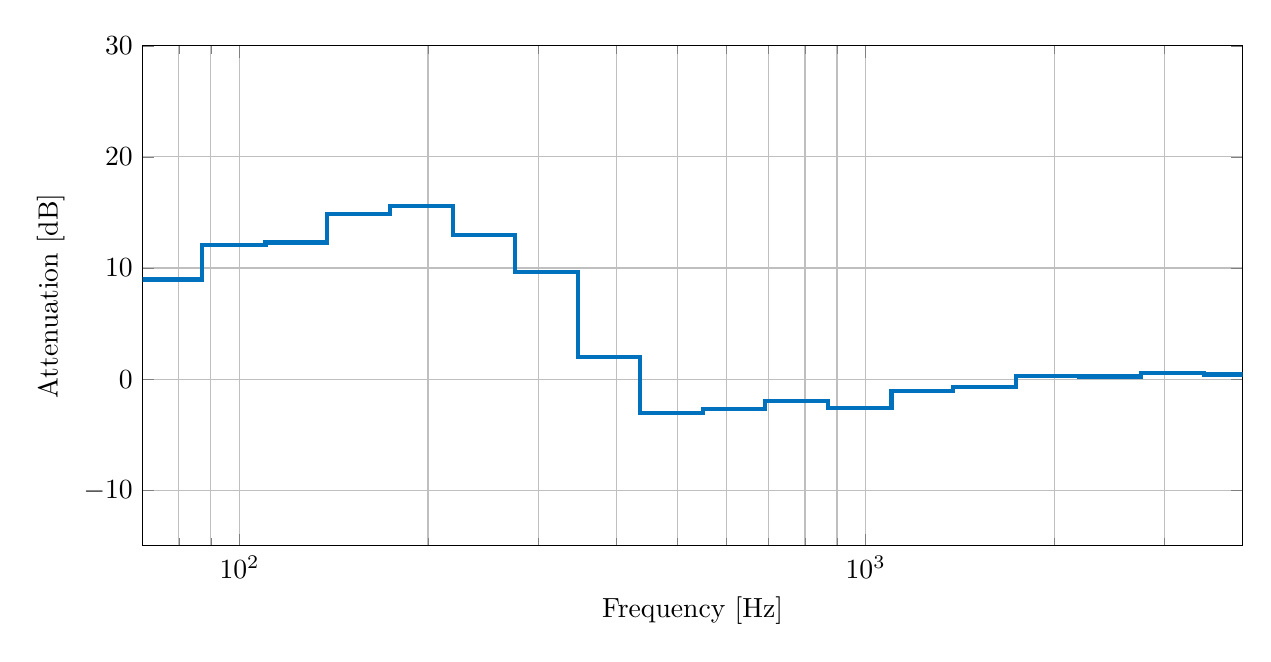
\begin{tikzpicture}

\begin{axis}[%
width=5.5in,
height=2.5in,
at={(1.011in,0.642in)},
scale only axis,
unbounded coords=jump,
xmode=log,
xmin=70,
xmax=4e+03,
xminorticks=true,
xlabel={Frequency [Hz]},
xmajorgrids,
xminorgrids,
ymin=-15,
ymax=30,
ylabel={Attenuation [dB]},
ymajorgrids,
axis background/.style={fill=white},
title style={font=\bfseries},
legend style={at={(0.03,0.03)},anchor=south west,legend cell align=left,align=left,draw=white!15!black}
]
\addplot[const plot,color=mycolor1,solid,forget plot,line width = 1.5pt] plot table[row sep=crcr] {%
	21.9	8.35\\
	27.5	6.3\\
	34.7	3.81\\
	43.6	5\\
	54.9	7.46\\
	69.1	8.97\\
	87.1	12.1\\
	110	12.3\\
	138	14.9\\
	174	15.6\\
	219	13\\
	275	9.65\\
	347	2.03\\
	436	-3.03\\
	549	-2.67\\
	691	-1.95\\
	871	-2.6\\
	1.1e+03	-1.03\\
	1.38e+03	-0.675\\
	1.74e+03	0.253\\
	2.19e+03	0.242\\
	2.75e+03	0.52\\
	3.47e+03	0.414\\
	4.36e+03	-0.138\\
	5.49e+03	-0.326\\
	6.91e+03	0.0245\\
	8.71e+03	0.299\\
	1.1e+04	0.251\\
	1.38e+04	0.132\\
	1.79e+04	0.0729\\
};
\end{axis}
\end{tikzpicture}%
	\caption{Denon AH GC20 measured in an anechoic chamber and averaged over five measurements, results were filtered using a 1/3 octave filter bank.}
	\label{fig:DenonComp}
\end{figure}

In figure \autoref{fig:OtherBrandsTestCompare} a comparison can be seen, this representation provides a better overview of the attenuation of four headphones.
\begin{figure}[H]
	\centering
	\tikzsetnextfilename{ComparedConusmerHPApp}
	% This file was created by matlab2tikz.
%
%The latest updates can be retrieved from
%  http://www.mathworks.com/matlabcentral/fileexchange/22022-matlab2tikz-matlab2tikz
%where you can also make suggestions and rate matlab2tikz.
%
\definecolor{mycolor1}{rgb}{0.00000,0.44700,0.74100}%
\definecolor{mycolor2}{rgb}{0.85000,0.32500,0.09800}%
\definecolor{mycolor3}{rgb}{0.92900,0.69400,0.12500}%
\definecolor{mycolor4}{rgb}{0.49400,0.18400,0.55600}%
%
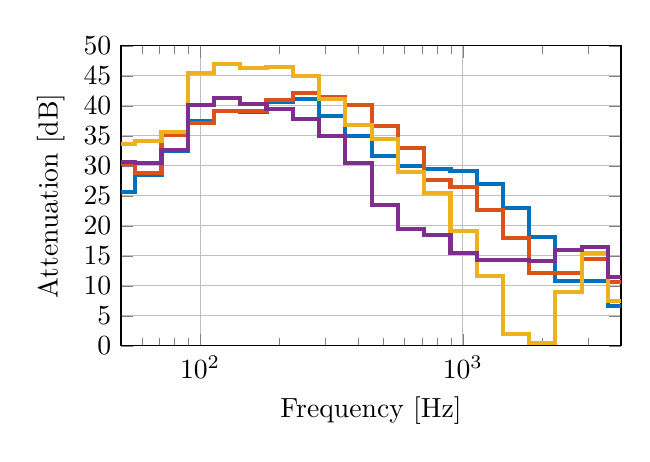
\begin{tikzpicture}

\begin{axis}[%
width=2.5in,
height=1.5in,
at={(1.011in,0.642in)},
scale only axis,
xmode=log,
xmin=50,
xmax=4000,
xlabel={Frequency [Hz]},
xmajorgrids,
%xmajorgrids,
%ymajorgrids,
%xminorgrids,
ymin=0,
ymax=50,
ytick={0,5,...,50},
ylabel={Attenuation [dB]},
ymajorgrids,
axis background/.style={fill=white},
title style={font=\bfseries},
%title={Comparison of Smoothened curves},
legend style={legend cell align=left,align=left,draw=white!15!black}
]
%\addplot[const plot,color=mycolor1,solid,forget plot,thick] plot table[row sep=crcr] {%
%	28.4	15.7\\
%	35.7	15.1\\
%	45	12.4\\
%	56.6	14\\
%	71.3	16.3\\
%	89.7	18.8\\
%	113	19.6\\
%	142	19.5\\
%	179	20.3\\
%	225	20.4\\
%	284	19.2\\
%	357	17.4\\
%	450	15.7\\
%	566	15.1\\
%	713	14.7\\
%	897	14.5\\
%	1.13e+03	13.5\\
%	1.42e+03	11.5\\
%	1.79e+03	9.08\\
%	2.25e+03	5.31\\
%	2.84e+03	5.51\\
%	3.57e+03	3.03\\
%	4.5e+03	2.37\\
%	5.66e+03	2.81\\
%	7.13e+03	3.07\\
%	8.97e+03	3.24\\
%	1.13e+04	1.16\\
%	1.42e+04	0.032\\
%	1.79e+04	0.598\\
%	2e+04	-0.763\\
%};
%\addplot[const plot,color=mycolor2,solid,forget plot,thick] plot table[row sep=crcr] {%
%	28.4	14.7\\
%	35.7	15.3\\
%	45	15.2\\
%	56.6	14.2\\
%	71.3	17.6\\
%	89.7	18.7\\
%	113	19.5\\
%	142	19.5\\
%	179	20.4\\
%	225	21.3\\
%	284	20.8\\
%	357	19.8\\
%	450	18.4\\
%	566	16.5\\
%	713	13.4\\
%	897	13.2\\
%	1.13e+03	11.4\\
%	1.42e+03	8.6\\
%	1.79e+03	6.11\\
%	2.25e+03	6.07\\
%	2.84e+03	7.27\\
%	3.57e+03	4.99\\
%	4.5e+03	2.6\\
%	5.66e+03	2.91\\
%	7.13e+03	1.03\\
%	8.97e+03	2.02\\
%	1.13e+04	-0.338\\
%	1.42e+04	-0.849\\
%	1.79e+04	-0.618\\
%	2e+04	-2.19\\
%};
%\addplot[const plot,color=mycolor3,solid,forget plot,thick] plot table[row sep=crcr] {%
%	28.4	18.1\\
%	35.7	19\\
%	45	17.1\\
%	56.6	16.5\\
%	71.3	18.6\\
%	89.7	22.8\\
%	113	23.6\\
%	142	23.3\\
%	179	23.5\\
%	225	22.6\\
%	284	20.4\\
%	357	18.4\\
%	450	17.2\\
%	566	14.5\\
%	713	12.7\\
%	897	9.48\\
%	1.13e+03	5.89\\
%	1.42e+03	1.04\\
%	1.79e+03	0.132\\
%	2.25e+03	4.45\\
%	2.84e+03	7.76\\
%	3.57e+03	3.73\\
%	4.5e+03	2.58\\
%	5.66e+03	2.46\\
%	7.13e+03	1.18\\
%	8.97e+03	1.16\\
%	1.13e+04	0.0281\\
%	1.42e+04	-0.34\\
%	1.79e+04	-0.623\\
%	2e+04	-1.08\\
%};
%\addplot[const plot,color=mycolor4,solid,forget plot,thick] plot table[row sep=crcr] {%
%	28.4	18.6\\
%	35.7	16.5\\
%	45	15.5\\
%	56.6	15.5\\
%	71.3	16.6\\
%	89.7	20.3\\
%	113	20.4\\
%	142	20\\
%	179	19.6\\
%	225	18.9\\
%	284	17.4\\
%	357	15.3\\
%	450	11.8\\
%	566	9.77\\
%	713	8.89\\
%	897	7.71\\
%	1.13e+03	6.86\\
%	1.42e+03	7.05\\
%	1.79e+03	7.37\\
%	2.25e+03	7.85\\
%	2.84e+03	8.24\\
%	3.57e+03	5.7\\
%	4.5e+03	3.78\\
%	5.66e+03	3.02\\
%	7.13e+03	1.43\\
%	8.97e+03	1.33\\
%	1.13e+04	1.58\\
%	1.42e+04	0.0462\\
%	1.79e+04	-1.02\\
%	2e+04	-0.621\\
%};
%\end{axis}

%% 20 log
\addplot[const plot,color=mycolor1,solid,line width=1.5pt,forget plot] plot table[row sep=crcr] {%
	28.4	30.6\\
	35.7	31.3\\
	45	25.7\\
	56.6	28.5\\
	71.3	32.4\\
	89.7	37.4\\
	113	39.1\\
	142	39\\
	179	40.6\\
	225	41.2\\
	284	38.3\\
	357	35\\
	450	31.7\\
	566	30\\
	713	29.4\\
	897	29.1\\
	1.13e+03	27\\
	1.42e+03	23\\
	1.79e+03	18.2\\
	2.25e+03	10.8\\
	2.84e+03	10.8\\
	3.57e+03	6.62\\
	4.5e+03	4.92\\
	5.66e+03	5.21\\
	7.13e+03	5.95\\
	8.97e+03	5.98\\
	1.13e+04	2.27\\
	1.42e+04	-1\\
	1.79e+04	0.842\\
	2e+04	-1.38\\
};
\addplot[const plot,color=mycolor2,solid,line width=1.5pt,forget plot] plot table[row sep=crcr] {%
	28.4	29.3\\
	35.7	30.1\\
	45	30.3\\
	56.6	28.8\\
	71.3	35.2\\
	89.7	37.2\\
	113	39.1\\
	142	39.2\\
	179	41\\
	225	42.2\\
	284	41.5\\
	357	40.1\\
	450	36.7\\
	566	33\\
	713	27.7\\
	897	26.5\\
	1.13e+03	22.7\\
	1.42e+03	17.9\\
	1.79e+03	12.1\\
	2.25e+03	12.1\\
	2.84e+03	14.4\\
	3.57e+03	10.6\\
	4.5e+03	5.72\\
	5.66e+03	5.17\\
	7.13e+03	2.13\\
	8.97e+03	4.17\\
	1.13e+04	-0.138\\
	1.42e+04	-0.907\\
	1.79e+04	-1.96\\
	2e+04	-4.33\\
};
\addplot[const plot,color=mycolor3,solid,line width=1.5pt,forget plot] plot table[row sep=crcr] {%
	28.4	36.2\\
	35.7	38.5\\
	45	33.6\\
	56.6	34.2\\
	71.3	35.6\\
	89.7	45.5\\
	113	46.9\\
	142	46.3\\
	179	46.5\\
	225	44.9\\
	284	41.1\\
	357	36.8\\
	450	34.5\\
	566	29\\
	713	25.5\\
	897	19.1\\
	1.13e+03	11.6\\
	1.42e+03	1.91\\
	1.79e+03	0.429\\
	2.25e+03	9.03\\
	2.84e+03	15.5\\
	3.57e+03	7.47\\
	4.5e+03	4.95\\
	5.66e+03	4.31\\
	7.13e+03	2.18\\
	8.97e+03	2.87\\
	1.13e+04	0.264\\
	1.42e+04	-0.554\\
	1.79e+04	-2.08\\
	2e+04	-2.36\\
};
\addplot[const plot,color=mycolor4,solid,line width=1.5pt,forget plot] plot table[row sep=crcr] {%
	28.4	37.2\\
	35.7	33.9\\
	45	30.7\\
	56.6	30.4\\
	71.3	32.7\\
	89.7	40.2\\
	113	41.3\\
	142	40.3\\
	179	39.5\\
	225	37.8\\
	284	34.9\\
	357	30.5\\
	450	23.4\\
	566	19.5\\
	713	18.4\\
	897	15.4\\
	1.13e+03	14.3\\
	1.42e+03	14.3\\
	1.79e+03	14.1\\
	2.25e+03	16\\
	2.84e+03	16.4\\
	3.57e+03	11.5\\
	4.5e+03	7.26\\
	5.66e+03	6.34\\
	7.13e+03	2.99\\
	8.97e+03	2.87\\
	1.13e+04	2.9\\
	1.42e+04	0.784\\
	1.79e+04	-1.51\\
	2e+04	-1.74\\
};
\end{axis}
\end{tikzpicture}%
	\caption{Denon AH-GC20(red), Bose QC25 (purple), Bose QC15(yellow) and B\&O H8(blue) measured in anechoic chamber, averaged over five measurements where the headphones was refitted between measurements.}
	\label{fig:OtherBrandsTestCompare}
\end{figure}


%\begin{figure}[H]
%	\centering
%	\tikzsetnextfilename{ComparedConusmerHPApp}
%	\input{../Journal/Experiments/TestofConsumerHeadphones/Plots/SmoothCompareAppendix(fig).tex}
%	\caption{Comparison of the Denon(blue), Bang \& Olufsen H8(red), Bose QC15(yellow) and Bose QC25(purple) fitted curves.}
%	\label{fig:OtherBrandsTestCompare}
%\end{figure}


\subsection{Conclusion}
The relative difference between a headphones attenuation with and without ANC was found for four different consumer headphones.



